\documentclass[twoside]{book}

% Packages required by doxygen
\usepackage{fixltx2e}
\usepackage{calc}
\usepackage{doxygen}
\usepackage[export]{adjustbox} % also loads graphicx
\usepackage{graphicx}
\usepackage[utf8]{inputenc}
\usepackage{makeidx}
\usepackage{multicol}
\usepackage{multirow}
\PassOptionsToPackage{warn}{textcomp}
\usepackage{textcomp}
\usepackage[nointegrals]{wasysym}
\usepackage[table]{xcolor}

% Font selection
\usepackage[T1]{fontenc}
\usepackage[scaled=.90]{helvet}
\usepackage{courier}
\usepackage{amssymb}
\usepackage{sectsty}
\renewcommand{\familydefault}{\sfdefault}
\allsectionsfont{%
  \fontseries{bc}\selectfont%
  \color{darkgray}%
}
\renewcommand{\DoxyLabelFont}{%
  \fontseries{bc}\selectfont%
  \color{darkgray}%
}
\newcommand{\+}{\discretionary{\mbox{\scriptsize$\hookleftarrow$}}{}{}}

% Page & text layout
\usepackage{geometry}
\geometry{%
  a4paper,%
  top=2.5cm,%
  bottom=2.5cm,%
  left=2.5cm,%
  right=2.5cm%
}
\tolerance=750
\hfuzz=15pt
\hbadness=750
\setlength{\emergencystretch}{15pt}
\setlength{\parindent}{0cm}
\setlength{\parskip}{3ex plus 2ex minus 2ex}
\makeatletter
\renewcommand{\paragraph}{%
  \@startsection{paragraph}{4}{0ex}{-1.0ex}{1.0ex}{%
    \normalfont\normalsize\bfseries\SS@parafont%
  }%
}
\renewcommand{\subparagraph}{%
  \@startsection{subparagraph}{5}{0ex}{-1.0ex}{1.0ex}{%
    \normalfont\normalsize\bfseries\SS@subparafont%
  }%
}
\makeatother

% Headers & footers
\usepackage{fancyhdr}
\pagestyle{fancyplain}
\fancyhead[LE]{\fancyplain{}{\bfseries\thepage}}
\fancyhead[CE]{\fancyplain{}{}}
\fancyhead[RE]{\fancyplain{}{\bfseries\leftmark}}
\fancyhead[LO]{\fancyplain{}{\bfseries\rightmark}}
\fancyhead[CO]{\fancyplain{}{}}
\fancyhead[RO]{\fancyplain{}{\bfseries\thepage}}
\fancyfoot[LE]{\fancyplain{}{}}
\fancyfoot[CE]{\fancyplain{}{}}
\fancyfoot[RE]{\fancyplain{}{\bfseries\scriptsize Generated by Doxygen }}
\fancyfoot[LO]{\fancyplain{}{\bfseries\scriptsize Generated by Doxygen }}
\fancyfoot[CO]{\fancyplain{}{}}
\fancyfoot[RO]{\fancyplain{}{}}
\renewcommand{\footrulewidth}{0.4pt}
\renewcommand{\chaptermark}[1]{%
  \markboth{#1}{}%
}
\renewcommand{\sectionmark}[1]{%
  \markright{\thesection\ #1}%
}

% Indices & bibliography
\usepackage{natbib}
\usepackage[titles]{tocloft}
\setcounter{tocdepth}{3}
\setcounter{secnumdepth}{5}
\makeindex

% Hyperlinks (required, but should be loaded last)
\usepackage{ifpdf}
\ifpdf
  \usepackage[pdftex,pagebackref=true]{hyperref}
\else
  \usepackage[ps2pdf,pagebackref=true]{hyperref}
\fi
\hypersetup{%
  colorlinks=true,%
  linkcolor=blue,%
  citecolor=blue,%
  unicode%
}

% Custom commands
\newcommand{\clearemptydoublepage}{%
  \newpage{\pagestyle{empty}\cleardoublepage}%
}

\usepackage{caption}
\captionsetup{labelsep=space,justification=centering,font={bf},singlelinecheck=off,skip=4pt,position=top}

%===== C O N T E N T S =====

\begin{document}

% Titlepage & ToC
\hypersetup{pageanchor=false,
             bookmarksnumbered=true,
             pdfencoding=unicode
            }
\pagenumbering{roman}
\begin{titlepage}
\vspace*{7cm}
\begin{center}%
{\Large Robotis Manipulator \\[1ex]\large 1.\+0.\+0 }\\
\vspace*{1cm}
{\large Generated by Doxygen 1.8.11}\\
\end{center}
\end{titlepage}
\clearemptydoublepage
\tableofcontents
\clearemptydoublepage
\pagenumbering{arabic}
\hypersetup{pageanchor=true}

%--- Begin generated contents ---
\chapter{Robotis Manipulator}
\label{index}\hypertarget{index}{}Robotis Manipulator is a library for controlling the manipulator provided by R\+O\+B\+O\+T\+IS. This library provides a manipulator class for setting manipulator parameters, and provides some math functions to configure the manipulator controller and a basic trajectory generators that uses minimum jerk. The user makes a class inheriting Robotis\+Manipulator class, and set up the class by using the provided functions and the vurtual classes. The class provides functions such as creating the trajectory, receiving joint positions from the actuators and sending the target positions to the actuators. The open\+\_\+manipulator\+\_\+libs package can be refer as an example. \begin{DoxyAuthor}{Authors}
Hye-\/\+Jong K\+IM \href{mailto:hjkim@robotis.com}{\tt hjkim@robotis.\+com}, Darby Lim \href{mailto:thlim@robotis.com}{\tt thlim@robotis.\+com}, Yong-\/\+Ho Na \href{mailto:yhna@robotis.com}{\tt yhna@robotis.\+com}, Ryan Shim \href{mailto:jhshim@robotis.com}{\tt jhshim@robotis.\+com} 
\end{DoxyAuthor}

\chapter{Robotis Manipulator}
\label{md_README}
\hypertarget{md_README}{}
\subsection*{R\+OS Packages for Robotis Manipulator}

\tabulinesep=1mm
\begin{longtabu} spread 0pt [c]{*3{|X[-1]}|}
\hline
\rowcolor{\tableheadbgcolor}\PBS\centering {\bf Version}&\PBS\centering {\bf Kinetic + Ubuntu Xenial}&\PBS\centering {\bf Melodic + Ubuntu Bionic  }\\\cline{1-3}
\endfirsthead
\hline
\endfoot
\hline
\rowcolor{\tableheadbgcolor}\PBS\centering {\bf Version}&\PBS\centering {\bf Kinetic + Ubuntu Xenial}&\PBS\centering {\bf Melodic + Ubuntu Bionic  }\\\cline{1-3}
\endhead
\PBS\centering \href{https://badge.fury.io/gh/ROBOTIS-GIT%2Frobotis_manipulator}{\tt }&\PBS\centering \href{https://travis-ci.org/ROBOTIS-GIT/robotis_manipulator}{\tt }&\PBS\centering \href{https://travis-ci.org/ROBOTIS-GIT/robotis_manipulator}{\tt } \\\cline{1-3}
\end{longtabu}
\subsection*{R\+O\+B\+O\+T\+IS e-\/\+Manual for Robotis Manipulator}


\begin{DoxyItemize}
\item \href{http://emanual.robotis.com/docs/en/platform/openmanipulator/}{\tt R\+O\+B\+O\+T\+IS e-\/\+Manual for Robotis Manipulator and Open\+Manipulator}
\end{DoxyItemize}

\subsection*{Wiki for \hyperlink{namespacerobotis__manipulator}{robotis\+\_\+manipulator} Packages}


\begin{DoxyItemize}
\item \href{http://wiki.ros.org/robotis_manipulator}{\tt http\+://wiki.\+ros.\+org/robotis\+\_\+manipulator}
\end{DoxyItemize}

\subsection*{Open Source related to Robotis Manipulator}


\begin{DoxyItemize}
\item \href{https://github.com/ROBOTIS-GIT/robotis_manipulator}{\tt robotis\+\_\+manipulator}
\item \href{https://github.com/ROBOTIS-GIT/open_manipulator}{\tt open\+\_\+manipulator}
\item \href{https://github.com/ROBOTIS-GIT/open_manipulator_msgs}{\tt open\+\_\+manipulator\+\_\+msgs}
\item \href{https://github.com/ROBOTIS-GIT/open_manipulator_simulations}{\tt open\+\_\+manipulator\+\_\+simulations}
\item \href{https://github.com/ROBOTIS-GIT/open_manipulator_perceptions}{\tt open\+\_\+manipulator\+\_\+perceptions}
\item \href{https://github.com/ROBOTIS-GIT/open_manipulator_processing}{\tt open\+\_\+manipulator\+\_\+processing}
\item \href{https://github.com/ROBOTIS-GIT/open_manipulator_friends}{\tt open\+\_\+manipulator\+\_\+friends}
\item \href{https://github.com/ROBOTIS-GIT/open_manipulator_with_tb3}{\tt open\+\_\+manipulator\+\_\+with\+\_\+tb3}
\item \href{https://github.com/ROBOTIS-GIT/open_manipulator_with_tb3_msgs}{\tt open\+\_\+manipulator\+\_\+with\+\_\+tb3\+\_\+msgs}
\item \href{https://github.com/ROBOTIS-GIT/open_manipulator_with_tb3_simulations}{\tt open\+\_\+manipulator\+\_\+with\+\_\+tb3\+\_\+simulations}
\item \href{https://github.com/ROBOTIS-GIT/OpenCR-Hardware}{\tt Open\+C\+R-\/\+Hardware}
\item \href{https://github.com/ROBOTIS-GIT/OpenCR}{\tt Open\+CR}
\end{DoxyItemize}

\subsection*{Documents and Videos related to Robotis Manipulator}


\begin{DoxyItemize}
\item \href{http://emanual.robotis.com/docs/en/platform/openmanipulator/}{\tt R\+O\+B\+O\+T\+IS e-\/\+Manual for Open\+Manipulator}
\item \href{http://emanual.robotis.com/docs/en/software/dynamixel/dynamixel_workbench/}{\tt R\+O\+B\+O\+T\+IS e-\/\+Manual for DYNMAIXEL Workbench}
\item \href{https://community.robotsource.org/t/download-the-ros-robot-programming-book-for-free/51/}{\tt e-\/\+Book for Turtle\+Bot3 and Open\+Manipulator}
\item \href{https://www.youtube.com/playlist?list=PLRG6WP3c31_WpEsB6_Rdt3KhiopXQlUkb}{\tt Videos for Open\+Manipulator}
\item \href{https://www.youtube.com/playlist?list=PLRG6WP3c31_XI3wlvHlx2Mp8BYqgqDURU}{\tt Videos for Turtle\+Bot3 and Open\+Manipulator} 
\end{DoxyItemize}

\chapter{Namespace Index}
\section{Namespace List}
Here is a list of all namespaces with brief descriptions\+:\begin{DoxyCompactList}
\item\contentsline{section}{\hyperlink{namespacerobotis__manipulator}{robotis\+\_\+manipulator} \\*Main namespace }{\pageref{namespacerobotis__manipulator}}{}
\item\contentsline{section}{\hyperlink{namespacerobotis__manipulator_1_1log}{robotis\+\_\+manipulator\+::log} }{\pageref{namespacerobotis__manipulator_1_1log}}{}
\item\contentsline{section}{\hyperlink{namespacerobotis__manipulator_1_1math}{robotis\+\_\+manipulator\+::math} }{\pageref{namespacerobotis__manipulator_1_1math}}{}
\end{DoxyCompactList}

\chapter{Class Index}
\section{Class List}
Here are the classes, structs, unions and interfaces with brief descriptions\+:\begin{DoxyCompactList}
\item\contentsline{section}{\hyperlink{structrobotis__manipulator_1_1_chaining_name}{robotis\+\_\+manipulator\+::\+Chaining\+Name} }{\pageref{structrobotis__manipulator_1_1_chaining_name}}{}
\item\contentsline{section}{\hyperlink{structrobotis__manipulator_1_1_component}{robotis\+\_\+manipulator\+::\+Component} }{\pageref{structrobotis__manipulator_1_1_component}}{}
\item\contentsline{section}{\hyperlink{classrobotis__manipulator_1_1_custom_joint_trajectory}{robotis\+\_\+manipulator\+::\+Custom\+Joint\+Trajectory} \\*The \hyperlink{classrobotis__manipulator_1_1_custom_joint_trajectory}{Custom\+Joint\+Trajectory} class }{\pageref{classrobotis__manipulator_1_1_custom_joint_trajectory}}{}
\item\contentsline{section}{\hyperlink{classrobotis__manipulator_1_1_custom_task_trajectory}{robotis\+\_\+manipulator\+::\+Custom\+Task\+Trajectory} \\*The \hyperlink{classrobotis__manipulator_1_1_custom_task_trajectory}{Custom\+Task\+Trajectory} class }{\pageref{classrobotis__manipulator_1_1_custom_task_trajectory}}{}
\item\contentsline{section}{\hyperlink{structrobotis__manipulator_1_1_dynamic_pose}{robotis\+\_\+manipulator\+::\+Dynamic\+Pose} }{\pageref{structrobotis__manipulator_1_1_dynamic_pose}}{}
\item\contentsline{section}{\hyperlink{structrobotis__manipulator_1_1_dynamicvector}{robotis\+\_\+manipulator\+::\+Dynamicvector} }{\pageref{structrobotis__manipulator_1_1_dynamicvector}}{}
\item\contentsline{section}{\hyperlink{structrobotis__manipulator_1_1_inertia}{robotis\+\_\+manipulator\+::\+Inertia} }{\pageref{structrobotis__manipulator_1_1_inertia}}{}
\item\contentsline{section}{\hyperlink{classrobotis__manipulator_1_1_joint_actuator}{robotis\+\_\+manipulator\+::\+Joint\+Actuator} \\*The \hyperlink{classrobotis__manipulator_1_1_joint_actuator}{Joint\+Actuator} class }{\pageref{classrobotis__manipulator_1_1_joint_actuator}}{}
\item\contentsline{section}{\hyperlink{structrobotis__manipulator_1_1_joint_constant}{robotis\+\_\+manipulator\+::\+Joint\+Constant} }{\pageref{structrobotis__manipulator_1_1_joint_constant}}{}
\item\contentsline{section}{\hyperlink{classrobotis__manipulator_1_1_joint_trajectory}{robotis\+\_\+manipulator\+::\+Joint\+Trajectory} \\*The \hyperlink{classrobotis__manipulator_1_1_joint_trajectory}{Joint\+Trajectory} class }{\pageref{classrobotis__manipulator_1_1_joint_trajectory}}{}
\item\contentsline{section}{\hyperlink{structrobotis__manipulator_1_1_kinematic_pose}{robotis\+\_\+manipulator\+::\+Kinematic\+Pose} }{\pageref{structrobotis__manipulator_1_1_kinematic_pose}}{}
\item\contentsline{section}{\hyperlink{classrobotis__manipulator_1_1_kinematics}{robotis\+\_\+manipulator\+::\+Kinematics} \\*The \hyperlink{classrobotis__manipulator_1_1_kinematics}{Kinematics} class }{\pageref{classrobotis__manipulator_1_1_kinematics}}{}
\item\contentsline{section}{\hyperlink{structrobotis__manipulator_1_1_limit}{robotis\+\_\+manipulator\+::\+Limit} }{\pageref{structrobotis__manipulator_1_1_limit}}{}
\item\contentsline{section}{\hyperlink{classrobotis__manipulator_1_1_manipulator}{robotis\+\_\+manipulator\+::\+Manipulator} \\*The \hyperlink{classrobotis__manipulator_1_1_manipulator}{Manipulator} class }{\pageref{classrobotis__manipulator_1_1_manipulator}}{}
\item\contentsline{section}{\hyperlink{classrobotis__manipulator_1_1_minimum_jerk}{robotis\+\_\+manipulator\+::\+Minimum\+Jerk} \\*The \hyperlink{classrobotis__manipulator_1_1_minimum_jerk}{Minimum\+Jerk} class }{\pageref{classrobotis__manipulator_1_1_minimum_jerk}}{}
\item\contentsline{section}{\hyperlink{structrobotis__manipulator_1_1_point}{robotis\+\_\+manipulator\+::\+Point} }{\pageref{structrobotis__manipulator_1_1_point}}{}
\item\contentsline{section}{\hyperlink{structrobotis__manipulator_1_1_pose}{robotis\+\_\+manipulator\+::\+Pose} }{\pageref{structrobotis__manipulator_1_1_pose}}{}
\item\contentsline{section}{\hyperlink{structrobotis__manipulator_1_1_relative}{robotis\+\_\+manipulator\+::\+Relative} }{\pageref{structrobotis__manipulator_1_1_relative}}{}
\item\contentsline{section}{\hyperlink{classrobotis__manipulator_1_1_robotis_manipulator}{robotis\+\_\+manipulator\+::\+Robotis\+Manipulator} \\*The \hyperlink{classrobotis__manipulator_1_1_robotis_manipulator}{Robotis\+Manipulator} class }{\pageref{classrobotis__manipulator_1_1_robotis_manipulator}}{}
\item\contentsline{section}{\hyperlink{classrobotis__manipulator_1_1_task_trajectory}{robotis\+\_\+manipulator\+::\+Task\+Trajectory} \\*The \hyperlink{classrobotis__manipulator_1_1_task_trajectory}{Task\+Trajectory} class }{\pageref{classrobotis__manipulator_1_1_task_trajectory}}{}
\item\contentsline{section}{\hyperlink{structrobotis__manipulator_1_1_time}{robotis\+\_\+manipulator\+::\+Time} }{\pageref{structrobotis__manipulator_1_1_time}}{}
\item\contentsline{section}{\hyperlink{classrobotis__manipulator_1_1_tool_actuator}{robotis\+\_\+manipulator\+::\+Tool\+Actuator} \\*The \hyperlink{classrobotis__manipulator_1_1_tool_actuator}{Tool\+Actuator} class }{\pageref{classrobotis__manipulator_1_1_tool_actuator}}{}
\item\contentsline{section}{\hyperlink{classrobotis__manipulator_1_1_trajectory}{robotis\+\_\+manipulator\+::\+Trajectory} \\*The \hyperlink{classrobotis__manipulator_1_1_trajectory}{Trajectory} class }{\pageref{classrobotis__manipulator_1_1_trajectory}}{}
\item\contentsline{section}{\hyperlink{structrobotis__manipulator_1_1_world}{robotis\+\_\+manipulator\+::\+World} }{\pageref{structrobotis__manipulator_1_1_world}}{}
\end{DoxyCompactList}

\chapter{File Index}
\section{File List}
Here is a list of all files with brief descriptions\+:\begin{DoxyCompactList}
\item\contentsline{section}{include/robotis\+\_\+manipulator/\hyperlink{robotis__manipulator_8h}{robotis\+\_\+manipulator.\+h} }{\pageref{robotis__manipulator_8h}}{}
\item\contentsline{section}{include/robotis\+\_\+manipulator/\hyperlink{robotis__manipulator__common_8h}{robotis\+\_\+manipulator\+\_\+common.\+h} }{\pageref{robotis__manipulator__common_8h}}{}
\item\contentsline{section}{include/robotis\+\_\+manipulator/\hyperlink{robotis__manipulator__log_8h}{robotis\+\_\+manipulator\+\_\+log.\+h} }{\pageref{robotis__manipulator__log_8h}}{}
\item\contentsline{section}{include/robotis\+\_\+manipulator/\hyperlink{robotis__manipulator__manager_8h}{robotis\+\_\+manipulator\+\_\+manager.\+h} }{\pageref{robotis__manipulator__manager_8h}}{}
\item\contentsline{section}{include/robotis\+\_\+manipulator/\hyperlink{robotis__manipulator__math_8h}{robotis\+\_\+manipulator\+\_\+math.\+h} }{\pageref{robotis__manipulator__math_8h}}{}
\item\contentsline{section}{include/robotis\+\_\+manipulator/\hyperlink{robotis__manipulator__trajectory__generator_8h}{robotis\+\_\+manipulator\+\_\+trajectory\+\_\+generator.\+h} }{\pageref{robotis__manipulator__trajectory__generator_8h}}{}
\item\contentsline{section}{src/\hyperlink{_robotis_manipulator_8h}{Robotis\+Manipulator.\+h} }{\pageref{_robotis_manipulator_8h}}{}
\item\contentsline{section}{src/robotis\+\_\+manipulator/\hyperlink{robotis__manipulator_8cpp}{robotis\+\_\+manipulator.\+cpp} }{\pageref{robotis__manipulator_8cpp}}{}
\item\contentsline{section}{src/robotis\+\_\+manipulator/\hyperlink{robotis__manipulator__common_8cpp}{robotis\+\_\+manipulator\+\_\+common.\+cpp} }{\pageref{robotis__manipulator__common_8cpp}}{}
\item\contentsline{section}{src/robotis\+\_\+manipulator/\hyperlink{robotis__manipulator__log_8cpp}{robotis\+\_\+manipulator\+\_\+log.\+cpp} }{\pageref{robotis__manipulator__log_8cpp}}{}
\item\contentsline{section}{src/robotis\+\_\+manipulator/\hyperlink{robotis__manipulator__manager_8cpp}{robotis\+\_\+manipulator\+\_\+manager.\+cpp} }{\pageref{robotis__manipulator__manager_8cpp}}{}
\item\contentsline{section}{src/robotis\+\_\+manipulator/\hyperlink{robotis__manipulator__math_8cpp}{robotis\+\_\+manipulator\+\_\+math.\+cpp} }{\pageref{robotis__manipulator__math_8cpp}}{}
\item\contentsline{section}{src/robotis\+\_\+manipulator/\hyperlink{robotis__manipulator__trajectory__generator_8cpp}{robotis\+\_\+manipulator\+\_\+trajectory\+\_\+generator.\+cpp} }{\pageref{robotis__manipulator__trajectory__generator_8cpp}}{}
\end{DoxyCompactList}

\chapter{Namespace Documentation}
\hypertarget{namespacerobotis__manipulator}{}\section{robotis\+\_\+manipulator Namespace Reference}
\label{namespacerobotis__manipulator}\index{robotis\+\_\+manipulator@{robotis\+\_\+manipulator}}


main namespace  


\subsection*{Namespaces}
\begin{DoxyCompactItemize}
\item 
 \hyperlink{namespacerobotis__manipulator_1_1log}{log}
\item 
 \hyperlink{namespacerobotis__manipulator_1_1math}{math}
\end{DoxyCompactItemize}
\subsection*{Classes}
\begin{DoxyCompactItemize}
\item 
struct \hyperlink{structrobotis__manipulator_1_1_chaining_name}{Chaining\+Name}
\item 
struct \hyperlink{structrobotis__manipulator_1_1_component}{Component}
\item 
class \hyperlink{classrobotis__manipulator_1_1_custom_joint_trajectory}{Custom\+Joint\+Trajectory}
\begin{DoxyCompactList}\small\item\em The \hyperlink{classrobotis__manipulator_1_1_custom_joint_trajectory}{Custom\+Joint\+Trajectory} class. \end{DoxyCompactList}\item 
class \hyperlink{classrobotis__manipulator_1_1_custom_task_trajectory}{Custom\+Task\+Trajectory}
\begin{DoxyCompactList}\small\item\em The \hyperlink{classrobotis__manipulator_1_1_custom_task_trajectory}{Custom\+Task\+Trajectory} class. \end{DoxyCompactList}\item 
struct \hyperlink{structrobotis__manipulator_1_1_dynamic_pose}{Dynamic\+Pose}
\item 
struct \hyperlink{structrobotis__manipulator_1_1_dynamicvector}{Dynamicvector}
\item 
struct \hyperlink{structrobotis__manipulator_1_1_inertia}{Inertia}
\item 
class \hyperlink{classrobotis__manipulator_1_1_joint_actuator}{Joint\+Actuator}
\begin{DoxyCompactList}\small\item\em The \hyperlink{classrobotis__manipulator_1_1_joint_actuator}{Joint\+Actuator} class. \end{DoxyCompactList}\item 
struct \hyperlink{structrobotis__manipulator_1_1_joint_constant}{Joint\+Constant}
\item 
class \hyperlink{classrobotis__manipulator_1_1_joint_trajectory}{Joint\+Trajectory}
\begin{DoxyCompactList}\small\item\em The \hyperlink{classrobotis__manipulator_1_1_joint_trajectory}{Joint\+Trajectory} class. \end{DoxyCompactList}\item 
struct \hyperlink{structrobotis__manipulator_1_1_kinematic_pose}{Kinematic\+Pose}
\item 
class \hyperlink{classrobotis__manipulator_1_1_kinematics}{Kinematics}
\begin{DoxyCompactList}\small\item\em The \hyperlink{classrobotis__manipulator_1_1_kinematics}{Kinematics} class. \end{DoxyCompactList}\item 
struct \hyperlink{structrobotis__manipulator_1_1_limit}{Limit}
\item 
class \hyperlink{classrobotis__manipulator_1_1_manipulator}{Manipulator}
\begin{DoxyCompactList}\small\item\em The \hyperlink{classrobotis__manipulator_1_1_manipulator}{Manipulator} class. \end{DoxyCompactList}\item 
class \hyperlink{classrobotis__manipulator_1_1_minimum_jerk}{Minimum\+Jerk}
\begin{DoxyCompactList}\small\item\em The \hyperlink{classrobotis__manipulator_1_1_minimum_jerk}{Minimum\+Jerk} class. \end{DoxyCompactList}\item 
struct \hyperlink{structrobotis__manipulator_1_1_point}{Point}
\item 
struct \hyperlink{structrobotis__manipulator_1_1_pose}{Pose}
\item 
struct \hyperlink{structrobotis__manipulator_1_1_relative}{Relative}
\item 
class \hyperlink{classrobotis__manipulator_1_1_robotis_manipulator}{Robotis\+Manipulator}
\begin{DoxyCompactList}\small\item\em The \hyperlink{classrobotis__manipulator_1_1_robotis_manipulator}{Robotis\+Manipulator} class. \end{DoxyCompactList}\item 
class \hyperlink{classrobotis__manipulator_1_1_task_trajectory}{Task\+Trajectory}
\begin{DoxyCompactList}\small\item\em The \hyperlink{classrobotis__manipulator_1_1_task_trajectory}{Task\+Trajectory} class. \end{DoxyCompactList}\item 
struct \hyperlink{structrobotis__manipulator_1_1_time}{Time}
\item 
class \hyperlink{classrobotis__manipulator_1_1_tool_actuator}{Tool\+Actuator}
\begin{DoxyCompactList}\small\item\em The \hyperlink{classrobotis__manipulator_1_1_tool_actuator}{Tool\+Actuator} class. \end{DoxyCompactList}\item 
class \hyperlink{classrobotis__manipulator_1_1_trajectory}{Trajectory}
\begin{DoxyCompactList}\small\item\em The \hyperlink{classrobotis__manipulator_1_1_trajectory}{Trajectory} class. \end{DoxyCompactList}\item 
struct \hyperlink{structrobotis__manipulator_1_1_world}{World}
\end{DoxyCompactItemize}
\subsection*{Typedefs}
\begin{DoxyCompactItemize}
\item 
typedef \hyperlink{robotis__manipulator__log_8h_a67f156408fa9d656017c406fe4f4b330}{S\+T\+R\+I\+NG} \hyperlink{namespacerobotis__manipulator_a08c2d25e77a01ad75b9bb740f8ce4765}{Name}
\item 
typedef struct \hyperlink{structrobotis__manipulator_1_1_kinematic_pose}{robotis\+\_\+manipulator\+::\+Kinematic\+Pose} \hyperlink{namespacerobotis__manipulator_ab1b7bd11d743d22bca6b64b3026d3ff0}{Kinematic\+Pose}
\item 
typedef struct \hyperlink{structrobotis__manipulator_1_1_dynamicvector}{robotis\+\_\+manipulator\+::\+Dynamicvector} \hyperlink{namespacerobotis__manipulator_a5b7433687a9ee2bad6b3340cdf211292}{Dynamicvector}
\item 
typedef struct \hyperlink{structrobotis__manipulator_1_1_dynamic_pose}{robotis\+\_\+manipulator\+::\+Dynamic\+Pose} \hyperlink{namespacerobotis__manipulator_a708cc4bcd2a495ef984c7a733666d088}{Dynamic\+Pose}
\item 
typedef struct \hyperlink{structrobotis__manipulator_1_1_inertia}{robotis\+\_\+manipulator\+::\+Inertia} \hyperlink{namespacerobotis__manipulator_a8c647a7589b972af5f7d31362b334be1}{Inertia}
\item 
typedef struct \hyperlink{structrobotis__manipulator_1_1_limit}{robotis\+\_\+manipulator\+::\+Limit} \hyperlink{namespacerobotis__manipulator_a1b399f654798ff0e3afb533d344d1485}{Limit}
\item 
typedef struct \hyperlink{structrobotis__manipulator_1_1_time}{robotis\+\_\+manipulator\+::\+Time} \hyperlink{namespacerobotis__manipulator_a1a7fc2145859dfbfbb20910e5373b7db}{Time}
\item 
typedef enum \hyperlink{namespacerobotis__manipulator_a008c110bef924df2737c5583000a9293}{robotis\+\_\+manipulator\+::\+Trajectory\+Type} \hyperlink{namespacerobotis__manipulator_adfa0c5066de3b85b33d8998df78f8c0e}{Trajectory\+Type}
\item 
typedef struct \hyperlink{structrobotis__manipulator_1_1_point}{robotis\+\_\+manipulator\+::\+Point} \hyperlink{namespacerobotis__manipulator_a14f99d40e3de0c0cc881b0b94504f99e}{Point}
\item 
typedef struct \hyperlink{structrobotis__manipulator_1_1_point}{robotis\+\_\+manipulator\+::\+Point} \hyperlink{namespacerobotis__manipulator_a26f478d98222f9ce1bf66c7df248037b}{Actuator\+Value}
\item 
typedef struct \hyperlink{structrobotis__manipulator_1_1_point}{robotis\+\_\+manipulator\+::\+Point} \hyperlink{namespacerobotis__manipulator_aa0556c98c5294ccf3a96c2d0fe315e40}{Joint\+Value}
\item 
typedef struct \hyperlink{structrobotis__manipulator_1_1_point}{robotis\+\_\+manipulator\+::\+Point} \hyperlink{namespacerobotis__manipulator_a54e0b849e686b7c6271dbe01d6ba6ef6}{Tool\+Value}
\item 
typedef std\+::vector$<$ \hyperlink{namespacerobotis__manipulator_aa0556c98c5294ccf3a96c2d0fe315e40}{Joint\+Value} $>$ \hyperlink{namespacerobotis__manipulator_a4456fd8b14e1f6b7733a77837dfe9339}{Joint\+Waypoint}
\item 
typedef struct \hyperlink{structrobotis__manipulator_1_1_pose}{robotis\+\_\+manipulator\+::\+Pose} \hyperlink{namespacerobotis__manipulator_a440e2d88ec85fdee394e540dc6024c3e}{Task\+Waypoint}
\item 
typedef struct \hyperlink{structrobotis__manipulator_1_1_pose}{robotis\+\_\+manipulator\+::\+Pose} \hyperlink{namespacerobotis__manipulator_a5934a151815a32d76af3af3bfe6e5be8}{Pose}
\item 
typedef enum \hyperlink{namespacerobotis__manipulator_a2bbf89d1c08dc1d9ff4e28beb939e382}{robotis\+\_\+manipulator\+::\+Component\+Type} \hyperlink{namespacerobotis__manipulator_a0074428cb994a4539fa1c1950d19db4c}{Component\+Type}
\item 
typedef struct \hyperlink{structrobotis__manipulator_1_1_chaining_name}{robotis\+\_\+manipulator\+::\+Chaining\+Name} \hyperlink{namespacerobotis__manipulator_a9b57e9a97855a185ca26900482155cdd}{Chaining\+Name}
\item 
typedef struct \hyperlink{structrobotis__manipulator_1_1_relative}{robotis\+\_\+manipulator\+::\+Relative} \hyperlink{namespacerobotis__manipulator_a62c82d0cc8d649345afd30cb34b32dd8}{Relative}
\item 
typedef struct \hyperlink{structrobotis__manipulator_1_1_joint_constant}{robotis\+\_\+manipulator\+::\+Joint\+Constant} \hyperlink{namespacerobotis__manipulator_aeefccd90c348d7afefbe86e8380227f9}{Joint\+Constant}
\item 
typedef struct \hyperlink{structrobotis__manipulator_1_1_world}{robotis\+\_\+manipulator\+::\+World} \hyperlink{namespacerobotis__manipulator_ad572cd4a47272e32196fdc45759963e3}{World}
\item 
typedef struct \hyperlink{structrobotis__manipulator_1_1_component}{robotis\+\_\+manipulator\+::\+Component} \hyperlink{namespacerobotis__manipulator_a66033834ce02ad7b8dec1a7228852657}{Component}
\end{DoxyCompactItemize}
\subsection*{Enumerations}
\begin{DoxyCompactItemize}
\item 
enum \hyperlink{namespacerobotis__manipulator_a008c110bef924df2737c5583000a9293}{Trajectory\+Type} \{ \\*
\hyperlink{namespacerobotis__manipulator_a008c110bef924df2737c5583000a9293abe18ccc5ef07711d5fec3eed3304d2fe}{N\+O\+NE} = 0, 
\hyperlink{namespacerobotis__manipulator_a008c110bef924df2737c5583000a9293a093d62b8684b778b26a1dc4a56239f3a}{J\+O\+I\+N\+T\+\_\+\+T\+R\+A\+J\+E\+C\+T\+O\+RY}, 
\hyperlink{namespacerobotis__manipulator_a008c110bef924df2737c5583000a9293ac3afdf4e66570420074ba4de482896c2}{T\+A\+S\+K\+\_\+\+T\+R\+A\+J\+E\+C\+T\+O\+RY}, 
\hyperlink{namespacerobotis__manipulator_a008c110bef924df2737c5583000a9293ae214e80a3aedf656b76a8863f0f9d169}{C\+U\+S\+T\+O\+M\+\_\+\+J\+O\+I\+N\+T\+\_\+\+T\+R\+A\+J\+E\+C\+T\+O\+RY}, 
\\*
\hyperlink{namespacerobotis__manipulator_a008c110bef924df2737c5583000a9293adda2674cede8ff709aa757c0b9e75c06}{C\+U\+S\+T\+O\+M\+\_\+\+T\+A\+S\+K\+\_\+\+T\+R\+A\+J\+E\+C\+T\+O\+RY}
 \}
\item 
enum \hyperlink{namespacerobotis__manipulator_a2bbf89d1c08dc1d9ff4e28beb939e382}{Component\+Type} \{ \hyperlink{namespacerobotis__manipulator_a2bbf89d1c08dc1d9ff4e28beb939e382a48d9e14bdd971b547f0b4bfcbf8588e7}{P\+A\+S\+S\+I\+V\+E\+\_\+\+J\+O\+I\+N\+T\+\_\+\+C\+O\+M\+P\+O\+N\+E\+NT} = 0, 
\hyperlink{namespacerobotis__manipulator_a2bbf89d1c08dc1d9ff4e28beb939e382acdf3b34914d1a2a028d882beb96fba7c}{A\+C\+T\+I\+V\+E\+\_\+\+J\+O\+I\+N\+T\+\_\+\+C\+O\+M\+P\+O\+N\+E\+NT}, 
\hyperlink{namespacerobotis__manipulator_a2bbf89d1c08dc1d9ff4e28beb939e382a7d53623544fe889894c54a988f503de0}{T\+O\+O\+L\+\_\+\+C\+O\+M\+P\+O\+N\+E\+NT}
 \}
\end{DoxyCompactItemize}


\subsection{Detailed Description}
main namespace 

\subsection{Typedef Documentation}
\index{robotis\+\_\+manipulator@{robotis\+\_\+manipulator}!Actuator\+Value@{Actuator\+Value}}
\index{Actuator\+Value@{Actuator\+Value}!robotis\+\_\+manipulator@{robotis\+\_\+manipulator}}
\subsubsection[{\texorpdfstring{Actuator\+Value}{ActuatorValue}}]{\setlength{\rightskip}{0pt plus 5cm}typedef struct {\bf robotis\+\_\+manipulator\+::\+Point}  {\bf robotis\+\_\+manipulator\+::\+Actuator\+Value}}\hypertarget{namespacerobotis__manipulator_a26f478d98222f9ce1bf66c7df248037b}{}\label{namespacerobotis__manipulator_a26f478d98222f9ce1bf66c7df248037b}
\index{robotis\+\_\+manipulator@{robotis\+\_\+manipulator}!Chaining\+Name@{Chaining\+Name}}
\index{Chaining\+Name@{Chaining\+Name}!robotis\+\_\+manipulator@{robotis\+\_\+manipulator}}
\subsubsection[{\texorpdfstring{Chaining\+Name}{ChainingName}}]{\setlength{\rightskip}{0pt plus 5cm}typedef struct {\bf robotis\+\_\+manipulator\+::\+Chaining\+Name}  {\bf robotis\+\_\+manipulator\+::\+Chaining\+Name}}\hypertarget{namespacerobotis__manipulator_a9b57e9a97855a185ca26900482155cdd}{}\label{namespacerobotis__manipulator_a9b57e9a97855a185ca26900482155cdd}
\index{robotis\+\_\+manipulator@{robotis\+\_\+manipulator}!Component@{Component}}
\index{Component@{Component}!robotis\+\_\+manipulator@{robotis\+\_\+manipulator}}
\subsubsection[{\texorpdfstring{Component}{Component}}]{\setlength{\rightskip}{0pt plus 5cm}typedef struct {\bf robotis\+\_\+manipulator\+::\+Component}  {\bf robotis\+\_\+manipulator\+::\+Component}}\hypertarget{namespacerobotis__manipulator_a66033834ce02ad7b8dec1a7228852657}{}\label{namespacerobotis__manipulator_a66033834ce02ad7b8dec1a7228852657}
\index{robotis\+\_\+manipulator@{robotis\+\_\+manipulator}!Component\+Type@{Component\+Type}}
\index{Component\+Type@{Component\+Type}!robotis\+\_\+manipulator@{robotis\+\_\+manipulator}}
\subsubsection[{\texorpdfstring{Component\+Type}{ComponentType}}]{\setlength{\rightskip}{0pt plus 5cm}typedef enum {\bf robotis\+\_\+manipulator\+::\+Component\+Type}  {\bf robotis\+\_\+manipulator\+::\+Component\+Type}}\hypertarget{namespacerobotis__manipulator_a0074428cb994a4539fa1c1950d19db4c}{}\label{namespacerobotis__manipulator_a0074428cb994a4539fa1c1950d19db4c}
\index{robotis\+\_\+manipulator@{robotis\+\_\+manipulator}!Dynamic\+Pose@{Dynamic\+Pose}}
\index{Dynamic\+Pose@{Dynamic\+Pose}!robotis\+\_\+manipulator@{robotis\+\_\+manipulator}}
\subsubsection[{\texorpdfstring{Dynamic\+Pose}{DynamicPose}}]{\setlength{\rightskip}{0pt plus 5cm}typedef struct {\bf robotis\+\_\+manipulator\+::\+Dynamic\+Pose}  {\bf robotis\+\_\+manipulator\+::\+Dynamic\+Pose}}\hypertarget{namespacerobotis__manipulator_a708cc4bcd2a495ef984c7a733666d088}{}\label{namespacerobotis__manipulator_a708cc4bcd2a495ef984c7a733666d088}
\index{robotis\+\_\+manipulator@{robotis\+\_\+manipulator}!Dynamicvector@{Dynamicvector}}
\index{Dynamicvector@{Dynamicvector}!robotis\+\_\+manipulator@{robotis\+\_\+manipulator}}
\subsubsection[{\texorpdfstring{Dynamicvector}{Dynamicvector}}]{\setlength{\rightskip}{0pt plus 5cm}typedef struct {\bf robotis\+\_\+manipulator\+::\+Dynamicvector}  {\bf robotis\+\_\+manipulator\+::\+Dynamicvector}}\hypertarget{namespacerobotis__manipulator_a5b7433687a9ee2bad6b3340cdf211292}{}\label{namespacerobotis__manipulator_a5b7433687a9ee2bad6b3340cdf211292}
\index{robotis\+\_\+manipulator@{robotis\+\_\+manipulator}!Inertia@{Inertia}}
\index{Inertia@{Inertia}!robotis\+\_\+manipulator@{robotis\+\_\+manipulator}}
\subsubsection[{\texorpdfstring{Inertia}{Inertia}}]{\setlength{\rightskip}{0pt plus 5cm}typedef struct {\bf robotis\+\_\+manipulator\+::\+Inertia}  {\bf robotis\+\_\+manipulator\+::\+Inertia}}\hypertarget{namespacerobotis__manipulator_a8c647a7589b972af5f7d31362b334be1}{}\label{namespacerobotis__manipulator_a8c647a7589b972af5f7d31362b334be1}
\index{robotis\+\_\+manipulator@{robotis\+\_\+manipulator}!Joint\+Constant@{Joint\+Constant}}
\index{Joint\+Constant@{Joint\+Constant}!robotis\+\_\+manipulator@{robotis\+\_\+manipulator}}
\subsubsection[{\texorpdfstring{Joint\+Constant}{JointConstant}}]{\setlength{\rightskip}{0pt plus 5cm}typedef struct {\bf robotis\+\_\+manipulator\+::\+Joint\+Constant}  {\bf robotis\+\_\+manipulator\+::\+Joint\+Constant}}\hypertarget{namespacerobotis__manipulator_aeefccd90c348d7afefbe86e8380227f9}{}\label{namespacerobotis__manipulator_aeefccd90c348d7afefbe86e8380227f9}
\index{robotis\+\_\+manipulator@{robotis\+\_\+manipulator}!Joint\+Value@{Joint\+Value}}
\index{Joint\+Value@{Joint\+Value}!robotis\+\_\+manipulator@{robotis\+\_\+manipulator}}
\subsubsection[{\texorpdfstring{Joint\+Value}{JointValue}}]{\setlength{\rightskip}{0pt plus 5cm}typedef struct {\bf robotis\+\_\+manipulator\+::\+Point}  {\bf robotis\+\_\+manipulator\+::\+Joint\+Value}}\hypertarget{namespacerobotis__manipulator_aa0556c98c5294ccf3a96c2d0fe315e40}{}\label{namespacerobotis__manipulator_aa0556c98c5294ccf3a96c2d0fe315e40}
\index{robotis\+\_\+manipulator@{robotis\+\_\+manipulator}!Joint\+Waypoint@{Joint\+Waypoint}}
\index{Joint\+Waypoint@{Joint\+Waypoint}!robotis\+\_\+manipulator@{robotis\+\_\+manipulator}}
\subsubsection[{\texorpdfstring{Joint\+Waypoint}{JointWaypoint}}]{\setlength{\rightskip}{0pt plus 5cm}typedef std\+::vector$<${\bf Joint\+Value}$>$ {\bf robotis\+\_\+manipulator\+::\+Joint\+Waypoint}}\hypertarget{namespacerobotis__manipulator_a4456fd8b14e1f6b7733a77837dfe9339}{}\label{namespacerobotis__manipulator_a4456fd8b14e1f6b7733a77837dfe9339}


Definition at line 114 of file robotis\+\_\+manipulator\+\_\+common.\+h.

\index{robotis\+\_\+manipulator@{robotis\+\_\+manipulator}!Kinematic\+Pose@{Kinematic\+Pose}}
\index{Kinematic\+Pose@{Kinematic\+Pose}!robotis\+\_\+manipulator@{robotis\+\_\+manipulator}}
\subsubsection[{\texorpdfstring{Kinematic\+Pose}{KinematicPose}}]{\setlength{\rightskip}{0pt plus 5cm}typedef struct {\bf robotis\+\_\+manipulator\+::\+Kinematic\+Pose}  {\bf robotis\+\_\+manipulator\+::\+Kinematic\+Pose}}\hypertarget{namespacerobotis__manipulator_ab1b7bd11d743d22bca6b64b3026d3ff0}{}\label{namespacerobotis__manipulator_ab1b7bd11d743d22bca6b64b3026d3ff0}
\index{robotis\+\_\+manipulator@{robotis\+\_\+manipulator}!Limit@{Limit}}
\index{Limit@{Limit}!robotis\+\_\+manipulator@{robotis\+\_\+manipulator}}
\subsubsection[{\texorpdfstring{Limit}{Limit}}]{\setlength{\rightskip}{0pt plus 5cm}typedef struct {\bf robotis\+\_\+manipulator\+::\+Limit}  {\bf robotis\+\_\+manipulator\+::\+Limit}}\hypertarget{namespacerobotis__manipulator_a1b399f654798ff0e3afb533d344d1485}{}\label{namespacerobotis__manipulator_a1b399f654798ff0e3afb533d344d1485}
\index{robotis\+\_\+manipulator@{robotis\+\_\+manipulator}!Name@{Name}}
\index{Name@{Name}!robotis\+\_\+manipulator@{robotis\+\_\+manipulator}}
\subsubsection[{\texorpdfstring{Name}{Name}}]{\setlength{\rightskip}{0pt plus 5cm}typedef {\bf S\+T\+R\+I\+NG} {\bf robotis\+\_\+manipulator\+::\+Name}}\hypertarget{namespacerobotis__manipulator_a08c2d25e77a01ad75b9bb740f8ce4765}{}\label{namespacerobotis__manipulator_a08c2d25e77a01ad75b9bb740f8ce4765}


Definition at line 46 of file robotis\+\_\+manipulator\+\_\+common.\+h.

\index{robotis\+\_\+manipulator@{robotis\+\_\+manipulator}!Point@{Point}}
\index{Point@{Point}!robotis\+\_\+manipulator@{robotis\+\_\+manipulator}}
\subsubsection[{\texorpdfstring{Point}{Point}}]{\setlength{\rightskip}{0pt plus 5cm}typedef struct {\bf robotis\+\_\+manipulator\+::\+Point}  {\bf robotis\+\_\+manipulator\+::\+Point}}\hypertarget{namespacerobotis__manipulator_a14f99d40e3de0c0cc881b0b94504f99e}{}\label{namespacerobotis__manipulator_a14f99d40e3de0c0cc881b0b94504f99e}
\index{robotis\+\_\+manipulator@{robotis\+\_\+manipulator}!Pose@{Pose}}
\index{Pose@{Pose}!robotis\+\_\+manipulator@{robotis\+\_\+manipulator}}
\subsubsection[{\texorpdfstring{Pose}{Pose}}]{\setlength{\rightskip}{0pt plus 5cm}typedef struct {\bf robotis\+\_\+manipulator\+::\+Pose}  {\bf robotis\+\_\+manipulator\+::\+Pose}}\hypertarget{namespacerobotis__manipulator_a5934a151815a32d76af3af3bfe6e5be8}{}\label{namespacerobotis__manipulator_a5934a151815a32d76af3af3bfe6e5be8}
\index{robotis\+\_\+manipulator@{robotis\+\_\+manipulator}!Relative@{Relative}}
\index{Relative@{Relative}!robotis\+\_\+manipulator@{robotis\+\_\+manipulator}}
\subsubsection[{\texorpdfstring{Relative}{Relative}}]{\setlength{\rightskip}{0pt plus 5cm}typedef struct {\bf robotis\+\_\+manipulator\+::\+Relative}  {\bf robotis\+\_\+manipulator\+::\+Relative}}\hypertarget{namespacerobotis__manipulator_a62c82d0cc8d649345afd30cb34b32dd8}{}\label{namespacerobotis__manipulator_a62c82d0cc8d649345afd30cb34b32dd8}
\index{robotis\+\_\+manipulator@{robotis\+\_\+manipulator}!Task\+Waypoint@{Task\+Waypoint}}
\index{Task\+Waypoint@{Task\+Waypoint}!robotis\+\_\+manipulator@{robotis\+\_\+manipulator}}
\subsubsection[{\texorpdfstring{Task\+Waypoint}{TaskWaypoint}}]{\setlength{\rightskip}{0pt plus 5cm}typedef struct {\bf robotis\+\_\+manipulator\+::\+Pose}  {\bf robotis\+\_\+manipulator\+::\+Task\+Waypoint}}\hypertarget{namespacerobotis__manipulator_a440e2d88ec85fdee394e540dc6024c3e}{}\label{namespacerobotis__manipulator_a440e2d88ec85fdee394e540dc6024c3e}
\index{robotis\+\_\+manipulator@{robotis\+\_\+manipulator}!Time@{Time}}
\index{Time@{Time}!robotis\+\_\+manipulator@{robotis\+\_\+manipulator}}
\subsubsection[{\texorpdfstring{Time}{Time}}]{\setlength{\rightskip}{0pt plus 5cm}typedef struct {\bf robotis\+\_\+manipulator\+::\+Time}  {\bf robotis\+\_\+manipulator\+::\+Time}}\hypertarget{namespacerobotis__manipulator_a1a7fc2145859dfbfbb20910e5373b7db}{}\label{namespacerobotis__manipulator_a1a7fc2145859dfbfbb20910e5373b7db}
\index{robotis\+\_\+manipulator@{robotis\+\_\+manipulator}!Tool\+Value@{Tool\+Value}}
\index{Tool\+Value@{Tool\+Value}!robotis\+\_\+manipulator@{robotis\+\_\+manipulator}}
\subsubsection[{\texorpdfstring{Tool\+Value}{ToolValue}}]{\setlength{\rightskip}{0pt plus 5cm}typedef struct {\bf robotis\+\_\+manipulator\+::\+Point}  {\bf robotis\+\_\+manipulator\+::\+Tool\+Value}}\hypertarget{namespacerobotis__manipulator_a54e0b849e686b7c6271dbe01d6ba6ef6}{}\label{namespacerobotis__manipulator_a54e0b849e686b7c6271dbe01d6ba6ef6}
\index{robotis\+\_\+manipulator@{robotis\+\_\+manipulator}!Trajectory\+Type@{Trajectory\+Type}}
\index{Trajectory\+Type@{Trajectory\+Type}!robotis\+\_\+manipulator@{robotis\+\_\+manipulator}}
\subsubsection[{\texorpdfstring{Trajectory\+Type}{TrajectoryType}}]{\setlength{\rightskip}{0pt plus 5cm}typedef enum {\bf robotis\+\_\+manipulator\+::\+Trajectory\+Type}  {\bf robotis\+\_\+manipulator\+::\+Trajectory\+Type}}\hypertarget{namespacerobotis__manipulator_adfa0c5066de3b85b33d8998df78f8c0e}{}\label{namespacerobotis__manipulator_adfa0c5066de3b85b33d8998df78f8c0e}
\index{robotis\+\_\+manipulator@{robotis\+\_\+manipulator}!World@{World}}
\index{World@{World}!robotis\+\_\+manipulator@{robotis\+\_\+manipulator}}
\subsubsection[{\texorpdfstring{World}{World}}]{\setlength{\rightskip}{0pt plus 5cm}typedef struct {\bf robotis\+\_\+manipulator\+::\+World}  {\bf robotis\+\_\+manipulator\+::\+World}}\hypertarget{namespacerobotis__manipulator_ad572cd4a47272e32196fdc45759963e3}{}\label{namespacerobotis__manipulator_ad572cd4a47272e32196fdc45759963e3}


\subsection{Enumeration Type Documentation}
\index{robotis\+\_\+manipulator@{robotis\+\_\+manipulator}!Component\+Type@{Component\+Type}}
\index{Component\+Type@{Component\+Type}!robotis\+\_\+manipulator@{robotis\+\_\+manipulator}}
\subsubsection[{\texorpdfstring{Component\+Type}{ComponentType}}]{\setlength{\rightskip}{0pt plus 5cm}enum {\bf robotis\+\_\+manipulator\+::\+Component\+Type}}\hypertarget{namespacerobotis__manipulator_a2bbf89d1c08dc1d9ff4e28beb939e382}{}\label{namespacerobotis__manipulator_a2bbf89d1c08dc1d9ff4e28beb939e382}
\begin{Desc}
\item[Enumerator]\par
\begin{description}
\index{P\+A\+S\+S\+I\+V\+E\+\_\+\+J\+O\+I\+N\+T\+\_\+\+C\+O\+M\+P\+O\+N\+E\+NT@{P\+A\+S\+S\+I\+V\+E\+\_\+\+J\+O\+I\+N\+T\+\_\+\+C\+O\+M\+P\+O\+N\+E\+NT}!robotis\+\_\+manipulator@{robotis\+\_\+manipulator}}\index{robotis\+\_\+manipulator@{robotis\+\_\+manipulator}!P\+A\+S\+S\+I\+V\+E\+\_\+\+J\+O\+I\+N\+T\+\_\+\+C\+O\+M\+P\+O\+N\+E\+NT@{P\+A\+S\+S\+I\+V\+E\+\_\+\+J\+O\+I\+N\+T\+\_\+\+C\+O\+M\+P\+O\+N\+E\+NT}}\item[{\em 
P\+A\+S\+S\+I\+V\+E\+\_\+\+J\+O\+I\+N\+T\+\_\+\+C\+O\+M\+P\+O\+N\+E\+NT\hypertarget{namespacerobotis__manipulator_a2bbf89d1c08dc1d9ff4e28beb939e382a48d9e14bdd971b547f0b4bfcbf8588e7}{}\label{namespacerobotis__manipulator_a2bbf89d1c08dc1d9ff4e28beb939e382a48d9e14bdd971b547f0b4bfcbf8588e7}
}]\index{A\+C\+T\+I\+V\+E\+\_\+\+J\+O\+I\+N\+T\+\_\+\+C\+O\+M\+P\+O\+N\+E\+NT@{A\+C\+T\+I\+V\+E\+\_\+\+J\+O\+I\+N\+T\+\_\+\+C\+O\+M\+P\+O\+N\+E\+NT}!robotis\+\_\+manipulator@{robotis\+\_\+manipulator}}\index{robotis\+\_\+manipulator@{robotis\+\_\+manipulator}!A\+C\+T\+I\+V\+E\+\_\+\+J\+O\+I\+N\+T\+\_\+\+C\+O\+M\+P\+O\+N\+E\+NT@{A\+C\+T\+I\+V\+E\+\_\+\+J\+O\+I\+N\+T\+\_\+\+C\+O\+M\+P\+O\+N\+E\+NT}}\item[{\em 
A\+C\+T\+I\+V\+E\+\_\+\+J\+O\+I\+N\+T\+\_\+\+C\+O\+M\+P\+O\+N\+E\+NT\hypertarget{namespacerobotis__manipulator_a2bbf89d1c08dc1d9ff4e28beb939e382acdf3b34914d1a2a028d882beb96fba7c}{}\label{namespacerobotis__manipulator_a2bbf89d1c08dc1d9ff4e28beb939e382acdf3b34914d1a2a028d882beb96fba7c}
}]\index{T\+O\+O\+L\+\_\+\+C\+O\+M\+P\+O\+N\+E\+NT@{T\+O\+O\+L\+\_\+\+C\+O\+M\+P\+O\+N\+E\+NT}!robotis\+\_\+manipulator@{robotis\+\_\+manipulator}}\index{robotis\+\_\+manipulator@{robotis\+\_\+manipulator}!T\+O\+O\+L\+\_\+\+C\+O\+M\+P\+O\+N\+E\+NT@{T\+O\+O\+L\+\_\+\+C\+O\+M\+P\+O\+N\+E\+NT}}\item[{\em 
T\+O\+O\+L\+\_\+\+C\+O\+M\+P\+O\+N\+E\+NT\hypertarget{namespacerobotis__manipulator_a2bbf89d1c08dc1d9ff4e28beb939e382a7d53623544fe889894c54a988f503de0}{}\label{namespacerobotis__manipulator_a2bbf89d1c08dc1d9ff4e28beb939e382a7d53623544fe889894c54a988f503de0}
}]\end{description}
\end{Desc}


Definition at line 126 of file robotis\+\_\+manipulator\+\_\+common.\+h.


\begin{DoxyCode}
127 \{
128   \hyperlink{namespacerobotis__manipulator_a2bbf89d1c08dc1d9ff4e28beb939e382a48d9e14bdd971b547f0b4bfcbf8588e7}{PASSIVE\_JOINT\_COMPONENT} = 0,
129   \hyperlink{namespacerobotis__manipulator_a2bbf89d1c08dc1d9ff4e28beb939e382acdf3b34914d1a2a028d882beb96fba7c}{ACTIVE\_JOINT\_COMPONENT},
130   \hyperlink{namespacerobotis__manipulator_a2bbf89d1c08dc1d9ff4e28beb939e382a7d53623544fe889894c54a988f503de0}{TOOL\_COMPONENT}
131 \} \hyperlink{namespacerobotis__manipulator_a0074428cb994a4539fa1c1950d19db4c}{ComponentType};
\end{DoxyCode}
\index{robotis\+\_\+manipulator@{robotis\+\_\+manipulator}!Trajectory\+Type@{Trajectory\+Type}}
\index{Trajectory\+Type@{Trajectory\+Type}!robotis\+\_\+manipulator@{robotis\+\_\+manipulator}}
\subsubsection[{\texorpdfstring{Trajectory\+Type}{TrajectoryType}}]{\setlength{\rightskip}{0pt plus 5cm}enum {\bf robotis\+\_\+manipulator\+::\+Trajectory\+Type}}\hypertarget{namespacerobotis__manipulator_a008c110bef924df2737c5583000a9293}{}\label{namespacerobotis__manipulator_a008c110bef924df2737c5583000a9293}
\begin{Desc}
\item[Enumerator]\par
\begin{description}
\index{N\+O\+NE@{N\+O\+NE}!robotis\+\_\+manipulator@{robotis\+\_\+manipulator}}\index{robotis\+\_\+manipulator@{robotis\+\_\+manipulator}!N\+O\+NE@{N\+O\+NE}}\item[{\em 
N\+O\+NE\hypertarget{namespacerobotis__manipulator_a008c110bef924df2737c5583000a9293abe18ccc5ef07711d5fec3eed3304d2fe}{}\label{namespacerobotis__manipulator_a008c110bef924df2737c5583000a9293abe18ccc5ef07711d5fec3eed3304d2fe}
}]\index{J\+O\+I\+N\+T\+\_\+\+T\+R\+A\+J\+E\+C\+T\+O\+RY@{J\+O\+I\+N\+T\+\_\+\+T\+R\+A\+J\+E\+C\+T\+O\+RY}!robotis\+\_\+manipulator@{robotis\+\_\+manipulator}}\index{robotis\+\_\+manipulator@{robotis\+\_\+manipulator}!J\+O\+I\+N\+T\+\_\+\+T\+R\+A\+J\+E\+C\+T\+O\+RY@{J\+O\+I\+N\+T\+\_\+\+T\+R\+A\+J\+E\+C\+T\+O\+RY}}\item[{\em 
J\+O\+I\+N\+T\+\_\+\+T\+R\+A\+J\+E\+C\+T\+O\+RY\hypertarget{namespacerobotis__manipulator_a008c110bef924df2737c5583000a9293a093d62b8684b778b26a1dc4a56239f3a}{}\label{namespacerobotis__manipulator_a008c110bef924df2737c5583000a9293a093d62b8684b778b26a1dc4a56239f3a}
}]\index{T\+A\+S\+K\+\_\+\+T\+R\+A\+J\+E\+C\+T\+O\+RY@{T\+A\+S\+K\+\_\+\+T\+R\+A\+J\+E\+C\+T\+O\+RY}!robotis\+\_\+manipulator@{robotis\+\_\+manipulator}}\index{robotis\+\_\+manipulator@{robotis\+\_\+manipulator}!T\+A\+S\+K\+\_\+\+T\+R\+A\+J\+E\+C\+T\+O\+RY@{T\+A\+S\+K\+\_\+\+T\+R\+A\+J\+E\+C\+T\+O\+RY}}\item[{\em 
T\+A\+S\+K\+\_\+\+T\+R\+A\+J\+E\+C\+T\+O\+RY\hypertarget{namespacerobotis__manipulator_a008c110bef924df2737c5583000a9293ac3afdf4e66570420074ba4de482896c2}{}\label{namespacerobotis__manipulator_a008c110bef924df2737c5583000a9293ac3afdf4e66570420074ba4de482896c2}
}]\index{C\+U\+S\+T\+O\+M\+\_\+\+J\+O\+I\+N\+T\+\_\+\+T\+R\+A\+J\+E\+C\+T\+O\+RY@{C\+U\+S\+T\+O\+M\+\_\+\+J\+O\+I\+N\+T\+\_\+\+T\+R\+A\+J\+E\+C\+T\+O\+RY}!robotis\+\_\+manipulator@{robotis\+\_\+manipulator}}\index{robotis\+\_\+manipulator@{robotis\+\_\+manipulator}!C\+U\+S\+T\+O\+M\+\_\+\+J\+O\+I\+N\+T\+\_\+\+T\+R\+A\+J\+E\+C\+T\+O\+RY@{C\+U\+S\+T\+O\+M\+\_\+\+J\+O\+I\+N\+T\+\_\+\+T\+R\+A\+J\+E\+C\+T\+O\+RY}}\item[{\em 
C\+U\+S\+T\+O\+M\+\_\+\+J\+O\+I\+N\+T\+\_\+\+T\+R\+A\+J\+E\+C\+T\+O\+RY\hypertarget{namespacerobotis__manipulator_a008c110bef924df2737c5583000a9293ae214e80a3aedf656b76a8863f0f9d169}{}\label{namespacerobotis__manipulator_a008c110bef924df2737c5583000a9293ae214e80a3aedf656b76a8863f0f9d169}
}]\index{C\+U\+S\+T\+O\+M\+\_\+\+T\+A\+S\+K\+\_\+\+T\+R\+A\+J\+E\+C\+T\+O\+RY@{C\+U\+S\+T\+O\+M\+\_\+\+T\+A\+S\+K\+\_\+\+T\+R\+A\+J\+E\+C\+T\+O\+RY}!robotis\+\_\+manipulator@{robotis\+\_\+manipulator}}\index{robotis\+\_\+manipulator@{robotis\+\_\+manipulator}!C\+U\+S\+T\+O\+M\+\_\+\+T\+A\+S\+K\+\_\+\+T\+R\+A\+J\+E\+C\+T\+O\+RY@{C\+U\+S\+T\+O\+M\+\_\+\+T\+A\+S\+K\+\_\+\+T\+R\+A\+J\+E\+C\+T\+O\+RY}}\item[{\em 
C\+U\+S\+T\+O\+M\+\_\+\+T\+A\+S\+K\+\_\+\+T\+R\+A\+J\+E\+C\+T\+O\+RY\hypertarget{namespacerobotis__manipulator_a008c110bef924df2737c5583000a9293adda2674cede8ff709aa757c0b9e75c06}{}\label{namespacerobotis__manipulator_a008c110bef924df2737c5583000a9293adda2674cede8ff709aa757c0b9e75c06}
}]\end{description}
\end{Desc}


Definition at line 97 of file robotis\+\_\+manipulator\+\_\+common.\+h.


\begin{DoxyCode}
98 \{
99   \hyperlink{namespacerobotis__manipulator_a008c110bef924df2737c5583000a9293abe18ccc5ef07711d5fec3eed3304d2fe}{NONE} = 0,
100   \hyperlink{namespacerobotis__manipulator_a008c110bef924df2737c5583000a9293a093d62b8684b778b26a1dc4a56239f3a}{JOINT\_TRAJECTORY},
101   \hyperlink{namespacerobotis__manipulator_a008c110bef924df2737c5583000a9293ac3afdf4e66570420074ba4de482896c2}{TASK\_TRAJECTORY},
102   \hyperlink{namespacerobotis__manipulator_a008c110bef924df2737c5583000a9293ae214e80a3aedf656b76a8863f0f9d169}{CUSTOM\_JOINT\_TRAJECTORY},
103   \hyperlink{namespacerobotis__manipulator_a008c110bef924df2737c5583000a9293adda2674cede8ff709aa757c0b9e75c06}{CUSTOM\_TASK\_TRAJECTORY}
104 \} \hyperlink{namespacerobotis__manipulator_adfa0c5066de3b85b33d8998df78f8c0e}{TrajectoryType};
\end{DoxyCode}

\hypertarget{namespacerobotis__manipulator_1_1log}{}\section{robotis\+\_\+manipulator\+:\+:log Namespace Reference}
\label{namespacerobotis__manipulator_1_1log}\index{robotis\+\_\+manipulator\+::log@{robotis\+\_\+manipulator\+::log}}
\subsection*{Functions}
\begin{DoxyCompactItemize}
\item 
void \hyperlink{namespacerobotis__manipulator_1_1log_ae01dad0f024eca3ad53f068204f6f293}{print} (\hyperlink{robotis__manipulator__log_8h_a67f156408fa9d656017c406fe4f4b330}{S\+T\+R\+I\+NG} str, \hyperlink{robotis__manipulator__log_8h_a67f156408fa9d656017c406fe4f4b330}{S\+T\+R\+I\+NG} color=\char`\"{}D\+E\+F\+A\+U\+LT\char`\"{})
\begin{DoxyCompactList}\small\item\em print \end{DoxyCompactList}\item 
void \hyperlink{namespacerobotis__manipulator_1_1log_ae2a75986a4f1075ab21646ff1fa5a21a}{print} (\hyperlink{robotis__manipulator__log_8h_a67f156408fa9d656017c406fe4f4b330}{S\+T\+R\+I\+NG} str, double data, uint8\+\_\+t decimal\+\_\+point=3, \hyperlink{robotis__manipulator__log_8h_a67f156408fa9d656017c406fe4f4b330}{S\+T\+R\+I\+NG} color=\char`\"{}D\+E\+F\+A\+U\+LT\char`\"{})
\begin{DoxyCompactList}\small\item\em print \end{DoxyCompactList}\item 
void \hyperlink{namespacerobotis__manipulator_1_1log_a8542b07bf2d0593a159d4e69cb19eceb}{print} (const char $\ast$str, \hyperlink{robotis__manipulator__log_8h_a67f156408fa9d656017c406fe4f4b330}{S\+T\+R\+I\+NG} color=\char`\"{}D\+E\+F\+A\+U\+LT\char`\"{})
\begin{DoxyCompactList}\small\item\em print \end{DoxyCompactList}\item 
void \hyperlink{namespacerobotis__manipulator_1_1log_a66839de0f964739cad9aa81383a9d651}{print} (const char $\ast$str, double data, uint8\+\_\+t decimal\+\_\+point=3, \hyperlink{robotis__manipulator__log_8h_a67f156408fa9d656017c406fe4f4b330}{S\+T\+R\+I\+NG} color=\char`\"{}D\+E\+F\+A\+U\+LT\char`\"{})
\begin{DoxyCompactList}\small\item\em print \end{DoxyCompactList}\item 
void \hyperlink{namespacerobotis__manipulator_1_1log_a4a6b5b7c361aa2c61631d2c2fcfdf065}{println} (\hyperlink{robotis__manipulator__log_8h_a67f156408fa9d656017c406fe4f4b330}{S\+T\+R\+I\+NG} str, \hyperlink{robotis__manipulator__log_8h_a67f156408fa9d656017c406fe4f4b330}{S\+T\+R\+I\+NG} color=\char`\"{}D\+E\+F\+A\+U\+LT\char`\"{})
\begin{DoxyCompactList}\small\item\em println \end{DoxyCompactList}\item 
void \hyperlink{namespacerobotis__manipulator_1_1log_a9e7dea27daabd2ac128133832a7e8db8}{println} (\hyperlink{robotis__manipulator__log_8h_a67f156408fa9d656017c406fe4f4b330}{S\+T\+R\+I\+NG} str, double data, uint8\+\_\+t decimal\+\_\+point=3, \hyperlink{robotis__manipulator__log_8h_a67f156408fa9d656017c406fe4f4b330}{S\+T\+R\+I\+NG} color=\char`\"{}D\+E\+F\+A\+U\+LT\char`\"{})
\begin{DoxyCompactList}\small\item\em println \end{DoxyCompactList}\item 
void \hyperlink{namespacerobotis__manipulator_1_1log_a950fa4b4f6a187c52e5d0721c1be551c}{println} (const char $\ast$str, \hyperlink{robotis__manipulator__log_8h_a67f156408fa9d656017c406fe4f4b330}{S\+T\+R\+I\+NG} color=\char`\"{}D\+E\+F\+A\+U\+LT\char`\"{})
\begin{DoxyCompactList}\small\item\em println \end{DoxyCompactList}\item 
void \hyperlink{namespacerobotis__manipulator_1_1log_a9582bb9bfbc4a4695975ed9e3320e3a0}{println} (const char $\ast$str, double data, uint8\+\_\+t decimal\+\_\+point=3, \hyperlink{robotis__manipulator__log_8h_a67f156408fa9d656017c406fe4f4b330}{S\+T\+R\+I\+NG} color=\char`\"{}D\+E\+F\+A\+U\+LT\char`\"{})
\begin{DoxyCompactList}\small\item\em println \end{DoxyCompactList}\item 
void \hyperlink{namespacerobotis__manipulator_1_1log_ae9b5a4788629e0abb0a29e2868d6d79e}{info} (\hyperlink{robotis__manipulator__log_8h_a67f156408fa9d656017c406fe4f4b330}{S\+T\+R\+I\+NG} str)
\begin{DoxyCompactList}\small\item\em info \end{DoxyCompactList}\item 
void \hyperlink{namespacerobotis__manipulator_1_1log_a530c16a6f6f6d7fe007ec32836af28a8}{info} (\hyperlink{robotis__manipulator__log_8h_a67f156408fa9d656017c406fe4f4b330}{S\+T\+R\+I\+NG} str, double data, uint8\+\_\+t decimal\+\_\+point=3)
\begin{DoxyCompactList}\small\item\em info \end{DoxyCompactList}\item 
void \hyperlink{namespacerobotis__manipulator_1_1log_a505032270cb596ee01dfc8e3030dc2c7}{info} (const char $\ast$str)
\begin{DoxyCompactList}\small\item\em info \end{DoxyCompactList}\item 
void \hyperlink{namespacerobotis__manipulator_1_1log_af5acc2141dc021f203cccc3ca3120d92}{info} (const char $\ast$str, double data, uint8\+\_\+t decimal\+\_\+point=3)
\begin{DoxyCompactList}\small\item\em info \end{DoxyCompactList}\item 
void \hyperlink{namespacerobotis__manipulator_1_1log_a0b7fa98d31c1beaf1c7d0989723a5fa2}{warn} (\hyperlink{robotis__manipulator__log_8h_a67f156408fa9d656017c406fe4f4b330}{S\+T\+R\+I\+NG} str)
\begin{DoxyCompactList}\small\item\em warn \end{DoxyCompactList}\item 
void \hyperlink{namespacerobotis__manipulator_1_1log_aac4f8d437de82deb67e7e9c4688dfcdc}{warn} (\hyperlink{robotis__manipulator__log_8h_a67f156408fa9d656017c406fe4f4b330}{S\+T\+R\+I\+NG} str, double data, uint8\+\_\+t decimal\+\_\+point=3)
\begin{DoxyCompactList}\small\item\em warn \end{DoxyCompactList}\item 
void \hyperlink{namespacerobotis__manipulator_1_1log_adcfad83d39b25e03a57b8cb20283606b}{warn} (const char $\ast$str)
\begin{DoxyCompactList}\small\item\em warn \end{DoxyCompactList}\item 
void \hyperlink{namespacerobotis__manipulator_1_1log_a6b4909ba686cc8ca3f5e4ee9b3eb5ec1}{warn} (const char $\ast$str, double data, uint8\+\_\+t decimal\+\_\+point=3)
\begin{DoxyCompactList}\small\item\em warn \end{DoxyCompactList}\item 
void \hyperlink{namespacerobotis__manipulator_1_1log_a6a84cb5481107ad244344093086fb557}{error} (\hyperlink{robotis__manipulator__log_8h_a67f156408fa9d656017c406fe4f4b330}{S\+T\+R\+I\+NG} str)
\begin{DoxyCompactList}\small\item\em error \end{DoxyCompactList}\item 
void \hyperlink{namespacerobotis__manipulator_1_1log_a2faeaa077a29ebfbdb2068f383574910}{error} (\hyperlink{robotis__manipulator__log_8h_a67f156408fa9d656017c406fe4f4b330}{S\+T\+R\+I\+NG} str, double data, uint8\+\_\+t decimal\+\_\+point=3)
\begin{DoxyCompactList}\small\item\em error \end{DoxyCompactList}\item 
void \hyperlink{namespacerobotis__manipulator_1_1log_a13df150c610fb95cf665a6d0673509b3}{error} (const char $\ast$str)
\begin{DoxyCompactList}\small\item\em error \end{DoxyCompactList}\item 
void \hyperlink{namespacerobotis__manipulator_1_1log_a19ab54a58a24d8f90c05cc10991561f4}{error} (const char $\ast$str, double data, uint8\+\_\+t decimal\+\_\+point=3)
\begin{DoxyCompactList}\small\item\em error \end{DoxyCompactList}\item 
{\footnotesize template$<$typename T $>$ }\\void \hyperlink{namespacerobotis__manipulator_1_1log_ab016bbac8ea97650fc14bd1be2ccdec5}{print\+\_\+vector} (std\+::vector$<$ T $>$ \&vec, uint8\+\_\+t decimal\+\_\+point=3)
\begin{DoxyCompactList}\small\item\em print\+\_\+vector \end{DoxyCompactList}\item 
{\footnotesize template$<$typename vector $>$ }\\void \hyperlink{namespacerobotis__manipulator_1_1log_a389a6cffbc5d0fad712e0eac8507a2ec}{print\+\_\+vector} (vector \&vec, uint8\+\_\+t decimal\+\_\+point=3)
\begin{DoxyCompactList}\small\item\em print\+\_\+vector \end{DoxyCompactList}\item 
{\footnotesize template$<$typename matrix $>$ }\\void \hyperlink{namespacerobotis__manipulator_1_1log_a84a7b621371c31dda949686b97b0d216}{print\+\_\+matrix} (matrix \&m, uint8\+\_\+t decimal\+\_\+point=3)
\begin{DoxyCompactList}\small\item\em print\+\_\+matrix \end{DoxyCompactList}\end{DoxyCompactItemize}


\subsection{Function Documentation}
\index{robotis\+\_\+manipulator\+::log@{robotis\+\_\+manipulator\+::log}!error@{error}}
\index{error@{error}!robotis\+\_\+manipulator\+::log@{robotis\+\_\+manipulator\+::log}}
\subsubsection[{\texorpdfstring{error(\+S\+T\+R\+I\+N\+G str)}{error(STRING str)}}]{\setlength{\rightskip}{0pt plus 5cm}void robotis\+\_\+manipulator\+::log\+::error (
\begin{DoxyParamCaption}
\item[{{\bf S\+T\+R\+I\+NG}}]{str}
\end{DoxyParamCaption}
)}\hypertarget{namespacerobotis__manipulator_1_1log_a6a84cb5481107ad244344093086fb557}{}\label{namespacerobotis__manipulator_1_1log_a6a84cb5481107ad244344093086fb557}


error 


\begin{DoxyParams}{Parameters}
{\em str} & \\
\hline
\end{DoxyParams}


Definition at line 239 of file robotis\+\_\+manipulator\+\_\+log.\+cpp.


\begin{DoxyCode}
240 \{
241 \textcolor{preprocessor}{#if defined(\_\_OPENCR\_\_)}
242   DEBUG.print(\textcolor{stringliteral}{"[ERROR] "});
243   DEBUG.println(str);
244 \textcolor{preprocessor}{#else}
245   printf(\hyperlink{robotis__manipulator__log_8h_a34995b955465f6bbb37c359173d50477}{ANSI\_COLOR\_RED});
246   printf(\textcolor{stringliteral}{"[ERROR] %s\(\backslash\)n"}, str.c\_str());
247   printf(\hyperlink{robotis__manipulator__log_8h_a92a364c2b863dde1a024a77eac2a5b3b}{ANSI\_COLOR\_RESET});
248 \textcolor{preprocessor}{#endif}
249 \}
\end{DoxyCode}


Here is the caller graph for this function\+:\nopagebreak
\begin{figure}[H]
\begin{center}
\leavevmode
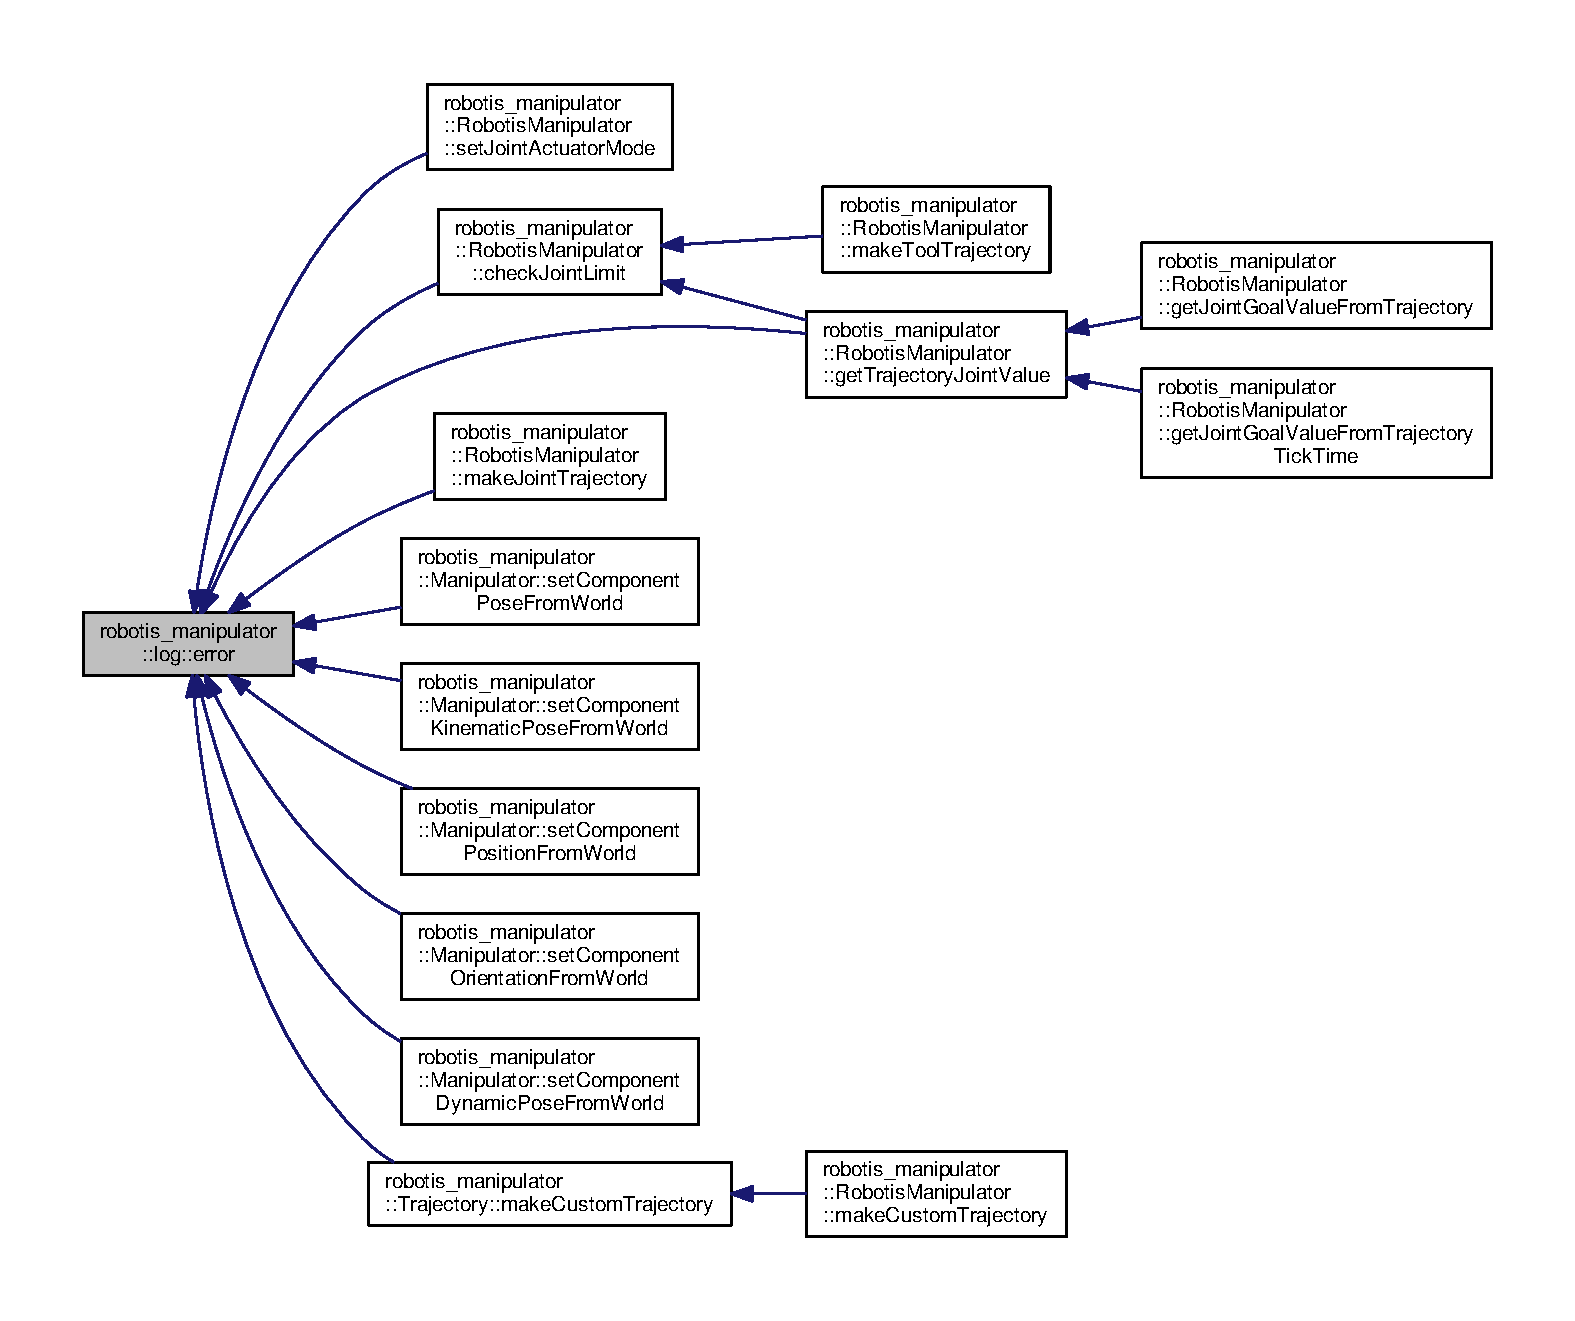
\includegraphics[width=350pt]{namespacerobotis__manipulator_1_1log_a6a84cb5481107ad244344093086fb557_icgraph}
\end{center}
\end{figure}


\index{robotis\+\_\+manipulator\+::log@{robotis\+\_\+manipulator\+::log}!error@{error}}
\index{error@{error}!robotis\+\_\+manipulator\+::log@{robotis\+\_\+manipulator\+::log}}
\subsubsection[{\texorpdfstring{error(\+S\+T\+R\+I\+N\+G str, double data, uint8\+\_\+t decimal\+\_\+point=3)}{error(STRING str, double data, uint8_t decimal_point=3)}}]{\setlength{\rightskip}{0pt plus 5cm}void robotis\+\_\+manipulator\+::log\+::error (
\begin{DoxyParamCaption}
\item[{{\bf S\+T\+R\+I\+NG}}]{str, }
\item[{double}]{data, }
\item[{uint8\+\_\+t}]{decimal\+\_\+point = {\ttfamily 3}}
\end{DoxyParamCaption}
)}\hypertarget{namespacerobotis__manipulator_1_1log_a2faeaa077a29ebfbdb2068f383574910}{}\label{namespacerobotis__manipulator_1_1log_a2faeaa077a29ebfbdb2068f383574910}


error 


\begin{DoxyParams}{Parameters}
{\em str} & \\
\hline
{\em data} & \\
\hline
{\em decimal\+\_\+point} & \\
\hline
\end{DoxyParams}


Definition at line 250 of file robotis\+\_\+manipulator\+\_\+log.\+cpp.


\begin{DoxyCode}
251 \{
252 \textcolor{preprocessor}{#if defined(\_\_OPENCR\_\_)}
253   DEBUG.print(\textcolor{stringliteral}{"[ERROR] "});
254   DEBUG.print(str);
255   DEBUG.println(data, decimal\_point);
256 \textcolor{preprocessor}{#else}
257   printf(\hyperlink{robotis__manipulator__log_8h_a34995b955465f6bbb37c359173d50477}{ANSI\_COLOR\_RED});
258   printf(\textcolor{stringliteral}{"[ERROR] %s %.*lf\(\backslash\)n"}, str.c\_str(), decimal\_point, data);
259   printf(\hyperlink{robotis__manipulator__log_8h_a92a364c2b863dde1a024a77eac2a5b3b}{ANSI\_COLOR\_RESET});
260 \textcolor{preprocessor}{#endif}
261 \}
\end{DoxyCode}
\index{robotis\+\_\+manipulator\+::log@{robotis\+\_\+manipulator\+::log}!error@{error}}
\index{error@{error}!robotis\+\_\+manipulator\+::log@{robotis\+\_\+manipulator\+::log}}
\subsubsection[{\texorpdfstring{error(const char $\ast$str)}{error(const char *str)}}]{\setlength{\rightskip}{0pt plus 5cm}void robotis\+\_\+manipulator\+::log\+::error (
\begin{DoxyParamCaption}
\item[{const char $\ast$}]{str}
\end{DoxyParamCaption}
)}\hypertarget{namespacerobotis__manipulator_1_1log_a13df150c610fb95cf665a6d0673509b3}{}\label{namespacerobotis__manipulator_1_1log_a13df150c610fb95cf665a6d0673509b3}


error 


\begin{DoxyParams}{Parameters}
{\em str} & \\
\hline
\end{DoxyParams}


Definition at line 263 of file robotis\+\_\+manipulator\+\_\+log.\+cpp.


\begin{DoxyCode}
264 \{
265 \textcolor{preprocessor}{#if defined(\_\_OPENCR\_\_)}
266   DEBUG.print(\textcolor{stringliteral}{"[ERROR] "});
267   DEBUG.println(str);
268 \textcolor{preprocessor}{#else}
269   printf(\hyperlink{robotis__manipulator__log_8h_a34995b955465f6bbb37c359173d50477}{ANSI\_COLOR\_RED});
270   printf(\textcolor{stringliteral}{"[ERROR] %s\(\backslash\)n"}, str);
271   printf(\hyperlink{robotis__manipulator__log_8h_a92a364c2b863dde1a024a77eac2a5b3b}{ANSI\_COLOR\_RESET});
272 \textcolor{preprocessor}{#endif}
273 \}
\end{DoxyCode}
\index{robotis\+\_\+manipulator\+::log@{robotis\+\_\+manipulator\+::log}!error@{error}}
\index{error@{error}!robotis\+\_\+manipulator\+::log@{robotis\+\_\+manipulator\+::log}}
\subsubsection[{\texorpdfstring{error(const char $\ast$str, double data, uint8\+\_\+t decimal\+\_\+point=3)}{error(const char *str, double data, uint8_t decimal_point=3)}}]{\setlength{\rightskip}{0pt plus 5cm}void robotis\+\_\+manipulator\+::log\+::error (
\begin{DoxyParamCaption}
\item[{const char $\ast$}]{str, }
\item[{double}]{data, }
\item[{uint8\+\_\+t}]{decimal\+\_\+point = {\ttfamily 3}}
\end{DoxyParamCaption}
)}\hypertarget{namespacerobotis__manipulator_1_1log_a19ab54a58a24d8f90c05cc10991561f4}{}\label{namespacerobotis__manipulator_1_1log_a19ab54a58a24d8f90c05cc10991561f4}


error 


\begin{DoxyParams}{Parameters}
{\em str} & \\
\hline
{\em data} & \\
\hline
{\em decimal\+\_\+point} & \\
\hline
\end{DoxyParams}


Definition at line 274 of file robotis\+\_\+manipulator\+\_\+log.\+cpp.


\begin{DoxyCode}
275 \{
276 \textcolor{preprocessor}{#if defined(\_\_OPENCR\_\_)}
277   DEBUG.print(\textcolor{stringliteral}{"[ERROR] "});
278   DEBUG.print(str);
279   DEBUG.println(data, decimal\_point);
280 \textcolor{preprocessor}{#else}
281   printf(\hyperlink{robotis__manipulator__log_8h_a34995b955465f6bbb37c359173d50477}{ANSI\_COLOR\_RED});
282   printf(\textcolor{stringliteral}{"[ERROR] %s %.*lf\(\backslash\)n"}, str, decimal\_point, data);
283   printf(\hyperlink{robotis__manipulator__log_8h_a92a364c2b863dde1a024a77eac2a5b3b}{ANSI\_COLOR\_RESET});
284 \textcolor{preprocessor}{#endif}
285 \}
\end{DoxyCode}
\index{robotis\+\_\+manipulator\+::log@{robotis\+\_\+manipulator\+::log}!info@{info}}
\index{info@{info}!robotis\+\_\+manipulator\+::log@{robotis\+\_\+manipulator\+::log}}
\subsubsection[{\texorpdfstring{info(\+S\+T\+R\+I\+N\+G str)}{info(STRING str)}}]{\setlength{\rightskip}{0pt plus 5cm}void robotis\+\_\+manipulator\+::log\+::info (
\begin{DoxyParamCaption}
\item[{{\bf S\+T\+R\+I\+NG}}]{str}
\end{DoxyParamCaption}
)}\hypertarget{namespacerobotis__manipulator_1_1log_ae9b5a4788629e0abb0a29e2868d6d79e}{}\label{namespacerobotis__manipulator_1_1log_ae9b5a4788629e0abb0a29e2868d6d79e}


info 


\begin{DoxyParams}{Parameters}
{\em str} & \\
\hline
\end{DoxyParams}


Definition at line 155 of file robotis\+\_\+manipulator\+\_\+log.\+cpp.


\begin{DoxyCode}
156 \{
157 \textcolor{preprocessor}{#if defined(\_\_OPENCR\_\_)}
158   DEBUG.print(\textcolor{stringliteral}{"[INFO] "});
159   DEBUG.println(str);
160 \textcolor{preprocessor}{#else}
161   printf(\textcolor{stringliteral}{"[INFO] %s\(\backslash\)n"}, str.c\_str());
162 \textcolor{preprocessor}{#endif}
163 \}
\end{DoxyCode}
\index{robotis\+\_\+manipulator\+::log@{robotis\+\_\+manipulator\+::log}!info@{info}}
\index{info@{info}!robotis\+\_\+manipulator\+::log@{robotis\+\_\+manipulator\+::log}}
\subsubsection[{\texorpdfstring{info(\+S\+T\+R\+I\+N\+G str, double data, uint8\+\_\+t decimal\+\_\+point=3)}{info(STRING str, double data, uint8_t decimal_point=3)}}]{\setlength{\rightskip}{0pt plus 5cm}void robotis\+\_\+manipulator\+::log\+::info (
\begin{DoxyParamCaption}
\item[{{\bf S\+T\+R\+I\+NG}}]{str, }
\item[{double}]{data, }
\item[{uint8\+\_\+t}]{decimal\+\_\+point = {\ttfamily 3}}
\end{DoxyParamCaption}
)}\hypertarget{namespacerobotis__manipulator_1_1log_a530c16a6f6f6d7fe007ec32836af28a8}{}\label{namespacerobotis__manipulator_1_1log_a530c16a6f6f6d7fe007ec32836af28a8}


info 


\begin{DoxyParams}{Parameters}
{\em str} & \\
\hline
{\em data} & \\
\hline
{\em decimal\+\_\+point} & \\
\hline
\end{DoxyParams}


Definition at line 164 of file robotis\+\_\+manipulator\+\_\+log.\+cpp.


\begin{DoxyCode}
165 \{
166 \textcolor{preprocessor}{#if defined(\_\_OPENCR\_\_)}
167   DEBUG.print(\textcolor{stringliteral}{"[INFO] "});
168   DEBUG.print(str);
169   DEBUG.println(data, decimal\_point);
170 \textcolor{preprocessor}{#else}
171   printf(\textcolor{stringliteral}{"[INFO] %s %.*lf\(\backslash\)n"}, str.c\_str(), decimal\_point, data);
172 \textcolor{preprocessor}{#endif}
173 \}
\end{DoxyCode}
\index{robotis\+\_\+manipulator\+::log@{robotis\+\_\+manipulator\+::log}!info@{info}}
\index{info@{info}!robotis\+\_\+manipulator\+::log@{robotis\+\_\+manipulator\+::log}}
\subsubsection[{\texorpdfstring{info(const char $\ast$str)}{info(const char *str)}}]{\setlength{\rightskip}{0pt plus 5cm}void robotis\+\_\+manipulator\+::log\+::info (
\begin{DoxyParamCaption}
\item[{const char $\ast$}]{str}
\end{DoxyParamCaption}
)}\hypertarget{namespacerobotis__manipulator_1_1log_a505032270cb596ee01dfc8e3030dc2c7}{}\label{namespacerobotis__manipulator_1_1log_a505032270cb596ee01dfc8e3030dc2c7}


info 


\begin{DoxyParams}{Parameters}
{\em str} & \\
\hline
\end{DoxyParams}


Definition at line 174 of file robotis\+\_\+manipulator\+\_\+log.\+cpp.


\begin{DoxyCode}
175 \{
176 \textcolor{preprocessor}{#if defined(\_\_OPENCR\_\_)}
177   DEBUG.print(\textcolor{stringliteral}{"[INFO] "});
178   DEBUG.println(str);
179 \textcolor{preprocessor}{#else}
180   printf(\textcolor{stringliteral}{"[INFO] %s\(\backslash\)n"}, str);
181 \textcolor{preprocessor}{#endif}
182 \}
\end{DoxyCode}
\index{robotis\+\_\+manipulator\+::log@{robotis\+\_\+manipulator\+::log}!info@{info}}
\index{info@{info}!robotis\+\_\+manipulator\+::log@{robotis\+\_\+manipulator\+::log}}
\subsubsection[{\texorpdfstring{info(const char $\ast$str, double data, uint8\+\_\+t decimal\+\_\+point=3)}{info(const char *str, double data, uint8_t decimal_point=3)}}]{\setlength{\rightskip}{0pt plus 5cm}void robotis\+\_\+manipulator\+::log\+::info (
\begin{DoxyParamCaption}
\item[{const char $\ast$}]{str, }
\item[{double}]{data, }
\item[{uint8\+\_\+t}]{decimal\+\_\+point = {\ttfamily 3}}
\end{DoxyParamCaption}
)}\hypertarget{namespacerobotis__manipulator_1_1log_af5acc2141dc021f203cccc3ca3120d92}{}\label{namespacerobotis__manipulator_1_1log_af5acc2141dc021f203cccc3ca3120d92}


info 


\begin{DoxyParams}{Parameters}
{\em str} & \\
\hline
{\em data} & \\
\hline
{\em decimal\+\_\+point} & \\
\hline
\end{DoxyParams}


Definition at line 183 of file robotis\+\_\+manipulator\+\_\+log.\+cpp.


\begin{DoxyCode}
184 \{
185 \textcolor{preprocessor}{#if defined(\_\_OPENCR\_\_)}
186   DEBUG.print(\textcolor{stringliteral}{"[INFO] "});
187   DEBUG.print(str);
188   DEBUG.println(data, decimal\_point);
189 \textcolor{preprocessor}{#else}
190   printf(\textcolor{stringliteral}{"[INFO] %s %.*lf\(\backslash\)n"}, str, decimal\_point, data);
191 \textcolor{preprocessor}{#endif}
192 \}
\end{DoxyCode}
\index{robotis\+\_\+manipulator\+::log@{robotis\+\_\+manipulator\+::log}!print@{print}}
\index{print@{print}!robotis\+\_\+manipulator\+::log@{robotis\+\_\+manipulator\+::log}}
\subsubsection[{\texorpdfstring{print(\+S\+T\+R\+I\+N\+G str, S\+T\+R\+I\+N\+G color=""D\+E\+F\+A\+U\+LT"")}{print(STRING str, STRING color="DEFAULT")}}]{\setlength{\rightskip}{0pt plus 5cm}void robotis\+\_\+manipulator\+::log\+::print (
\begin{DoxyParamCaption}
\item[{{\bf S\+T\+R\+I\+NG}}]{str, }
\item[{{\bf S\+T\+R\+I\+NG}}]{color = {\ttfamily \char`\"{}DEFAULT\char`\"{}}}
\end{DoxyParamCaption}
)}\hypertarget{namespacerobotis__manipulator_1_1log_ae01dad0f024eca3ad53f068204f6f293}{}\label{namespacerobotis__manipulator_1_1log_ae01dad0f024eca3ad53f068204f6f293}


print 


\begin{DoxyParams}{Parameters}
{\em str} & \\
\hline
{\em color} & \\
\hline
\end{DoxyParams}


Definition at line 28 of file robotis\+\_\+manipulator\+\_\+log.\+cpp.


\begin{DoxyCode}
29 \{
30 \textcolor{preprocessor}{#if defined(\_\_OPENCR\_\_)}
31   DEBUG.print(str);
32 \textcolor{preprocessor}{#else}
33        \textcolor{keywordflow}{if}(color == \textcolor{stringliteral}{"RED"})      printf(\hyperlink{robotis__manipulator__log_8h_a34995b955465f6bbb37c359173d50477}{ANSI\_COLOR\_RED});
34   \textcolor{keywordflow}{else} \textcolor{keywordflow}{if}(color == \textcolor{stringliteral}{"GREEN"})    printf(\hyperlink{robotis__manipulator__log_8h_a966c72d8d733c7734c6c784753d894c7}{ANSI\_COLOR\_GREEN});
35   \textcolor{keywordflow}{else} \textcolor{keywordflow}{if}(color == \textcolor{stringliteral}{"YELLOW"})   printf(\hyperlink{robotis__manipulator__log_8h_a5a123b382640b3aa65dd5db386002fbc}{ANSI\_COLOR\_YELLOW});
36   \textcolor{keywordflow}{else} \textcolor{keywordflow}{if}(color == \textcolor{stringliteral}{"BLUE"})     printf(\hyperlink{robotis__manipulator__log_8h_aca16e6a49eb51333c5fd3eee19487315}{ANSI\_COLOR\_BLUE});
37   \textcolor{keywordflow}{else} \textcolor{keywordflow}{if}(color == \textcolor{stringliteral}{"MAGENTA"})  printf(\hyperlink{robotis__manipulator__log_8h_acb30614ba1535da5b9d0c490b3c10515}{ANSI\_COLOR\_MAGENTA});
38   \textcolor{keywordflow}{else} \textcolor{keywordflow}{if}(color == \textcolor{stringliteral}{"CYAN"})     printf(\hyperlink{robotis__manipulator__log_8h_a8d0b0043e152438bb39b918a1f98c65f}{ANSI\_COLOR\_CYAN});
39   printf(\textcolor{stringliteral}{"%s"}, str.c\_str());
40   printf(\hyperlink{robotis__manipulator__log_8h_a92a364c2b863dde1a024a77eac2a5b3b}{ANSI\_COLOR\_RESET});
41 \textcolor{preprocessor}{#endif}
42 \}
\end{DoxyCode}


Here is the caller graph for this function\+:\nopagebreak
\begin{figure}[H]
\begin{center}
\leavevmode
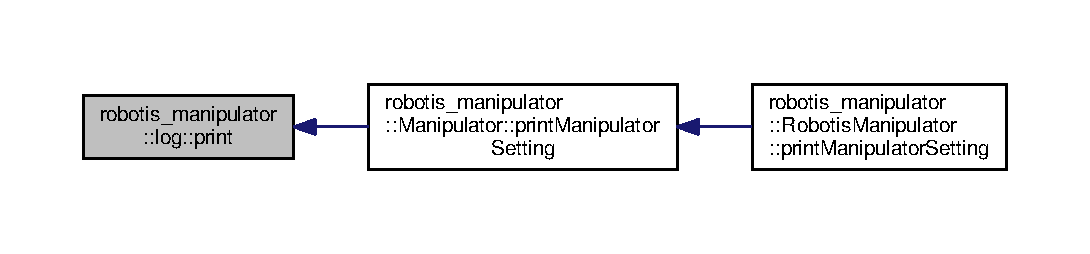
\includegraphics[width=350pt]{namespacerobotis__manipulator_1_1log_ae01dad0f024eca3ad53f068204f6f293_icgraph}
\end{center}
\end{figure}


\index{robotis\+\_\+manipulator\+::log@{robotis\+\_\+manipulator\+::log}!print@{print}}
\index{print@{print}!robotis\+\_\+manipulator\+::log@{robotis\+\_\+manipulator\+::log}}
\subsubsection[{\texorpdfstring{print(\+S\+T\+R\+I\+N\+G str, double data, uint8\+\_\+t decimal\+\_\+point=3, S\+T\+R\+I\+N\+G color=""D\+E\+F\+A\+U\+LT"")}{print(STRING str, double data, uint8_t decimal_point=3, STRING color="DEFAULT")}}]{\setlength{\rightskip}{0pt plus 5cm}void robotis\+\_\+manipulator\+::log\+::print (
\begin{DoxyParamCaption}
\item[{{\bf S\+T\+R\+I\+NG}}]{str, }
\item[{double}]{data, }
\item[{uint8\+\_\+t}]{decimal\+\_\+point = {\ttfamily 3}, }
\item[{{\bf S\+T\+R\+I\+NG}}]{color = {\ttfamily \char`\"{}DEFAULT\char`\"{}}}
\end{DoxyParamCaption}
)}\hypertarget{namespacerobotis__manipulator_1_1log_ae2a75986a4f1075ab21646ff1fa5a21a}{}\label{namespacerobotis__manipulator_1_1log_ae2a75986a4f1075ab21646ff1fa5a21a}


print 


\begin{DoxyParams}{Parameters}
{\em str} & \\
\hline
{\em data} & \\
\hline
{\em decimal\+\_\+point} & \\
\hline
{\em color} & \\
\hline
\end{DoxyParams}


Definition at line 43 of file robotis\+\_\+manipulator\+\_\+log.\+cpp.


\begin{DoxyCode}
44 \{
45 \textcolor{preprocessor}{#if defined(\_\_OPENCR\_\_)}
46   DEBUG.print(str);
47   DEBUG.print(data, decimal\_point);
48 \textcolor{preprocessor}{#else}
49        \textcolor{keywordflow}{if}(color == \textcolor{stringliteral}{"RED"})      printf(\hyperlink{robotis__manipulator__log_8h_a34995b955465f6bbb37c359173d50477}{ANSI\_COLOR\_RED});
50   \textcolor{keywordflow}{else} \textcolor{keywordflow}{if}(color == \textcolor{stringliteral}{"GREEN"})    printf(\hyperlink{robotis__manipulator__log_8h_a966c72d8d733c7734c6c784753d894c7}{ANSI\_COLOR\_GREEN});
51   \textcolor{keywordflow}{else} \textcolor{keywordflow}{if}(color == \textcolor{stringliteral}{"YELLOW"})   printf(\hyperlink{robotis__manipulator__log_8h_a5a123b382640b3aa65dd5db386002fbc}{ANSI\_COLOR\_YELLOW});
52   \textcolor{keywordflow}{else} \textcolor{keywordflow}{if}(color == \textcolor{stringliteral}{"BLUE"})     printf(\hyperlink{robotis__manipulator__log_8h_aca16e6a49eb51333c5fd3eee19487315}{ANSI\_COLOR\_BLUE});
53   \textcolor{keywordflow}{else} \textcolor{keywordflow}{if}(color == \textcolor{stringliteral}{"MAGENTA"})  printf(\hyperlink{robotis__manipulator__log_8h_acb30614ba1535da5b9d0c490b3c10515}{ANSI\_COLOR\_MAGENTA});
54   \textcolor{keywordflow}{else} \textcolor{keywordflow}{if}(color == \textcolor{stringliteral}{"CYAN"})     printf(\hyperlink{robotis__manipulator__log_8h_a8d0b0043e152438bb39b918a1f98c65f}{ANSI\_COLOR\_CYAN});
55   printf(\textcolor{stringliteral}{"%s %.*lf"}, str.c\_str(), decimal\_point, data);
56   printf(\hyperlink{robotis__manipulator__log_8h_a92a364c2b863dde1a024a77eac2a5b3b}{ANSI\_COLOR\_RESET});
57 \textcolor{preprocessor}{#endif}
58 \}
\end{DoxyCode}
\index{robotis\+\_\+manipulator\+::log@{robotis\+\_\+manipulator\+::log}!print@{print}}
\index{print@{print}!robotis\+\_\+manipulator\+::log@{robotis\+\_\+manipulator\+::log}}
\subsubsection[{\texorpdfstring{print(const char $\ast$str, S\+T\+R\+I\+N\+G color=""D\+E\+F\+A\+U\+LT"")}{print(const char *str, STRING color="DEFAULT")}}]{\setlength{\rightskip}{0pt plus 5cm}void robotis\+\_\+manipulator\+::log\+::print (
\begin{DoxyParamCaption}
\item[{const char $\ast$}]{str, }
\item[{{\bf S\+T\+R\+I\+NG}}]{color = {\ttfamily \char`\"{}DEFAULT\char`\"{}}}
\end{DoxyParamCaption}
)}\hypertarget{namespacerobotis__manipulator_1_1log_a8542b07bf2d0593a159d4e69cb19eceb}{}\label{namespacerobotis__manipulator_1_1log_a8542b07bf2d0593a159d4e69cb19eceb}


print 


\begin{DoxyParams}{Parameters}
{\em str} & \\
\hline
{\em color} & \\
\hline
\end{DoxyParams}


Definition at line 59 of file robotis\+\_\+manipulator\+\_\+log.\+cpp.


\begin{DoxyCode}
60 \{
61 \textcolor{preprocessor}{#if defined(\_\_OPENCR\_\_)}
62   DEBUG.print(str);
63 \textcolor{preprocessor}{#else}
64        \textcolor{keywordflow}{if}(color == \textcolor{stringliteral}{"RED"})      printf(\hyperlink{robotis__manipulator__log_8h_a34995b955465f6bbb37c359173d50477}{ANSI\_COLOR\_RED});
65   \textcolor{keywordflow}{else} \textcolor{keywordflow}{if}(color == \textcolor{stringliteral}{"GREEN"})    printf(\hyperlink{robotis__manipulator__log_8h_a966c72d8d733c7734c6c784753d894c7}{ANSI\_COLOR\_GREEN});
66   \textcolor{keywordflow}{else} \textcolor{keywordflow}{if}(color == \textcolor{stringliteral}{"YELLOW"})   printf(\hyperlink{robotis__manipulator__log_8h_a5a123b382640b3aa65dd5db386002fbc}{ANSI\_COLOR\_YELLOW});
67   \textcolor{keywordflow}{else} \textcolor{keywordflow}{if}(color == \textcolor{stringliteral}{"BLUE"})     printf(\hyperlink{robotis__manipulator__log_8h_aca16e6a49eb51333c5fd3eee19487315}{ANSI\_COLOR\_BLUE});
68   \textcolor{keywordflow}{else} \textcolor{keywordflow}{if}(color == \textcolor{stringliteral}{"MAGENTA"})  printf(\hyperlink{robotis__manipulator__log_8h_acb30614ba1535da5b9d0c490b3c10515}{ANSI\_COLOR\_MAGENTA});
69   \textcolor{keywordflow}{else} \textcolor{keywordflow}{if}(color == \textcolor{stringliteral}{"CYAN"})     printf(\hyperlink{robotis__manipulator__log_8h_a8d0b0043e152438bb39b918a1f98c65f}{ANSI\_COLOR\_CYAN});
70   printf(\textcolor{stringliteral}{"%s"}, str);
71   printf(\hyperlink{robotis__manipulator__log_8h_a92a364c2b863dde1a024a77eac2a5b3b}{ANSI\_COLOR\_RESET});
72 \textcolor{preprocessor}{#endif}
73 \}
\end{DoxyCode}
\index{robotis\+\_\+manipulator\+::log@{robotis\+\_\+manipulator\+::log}!print@{print}}
\index{print@{print}!robotis\+\_\+manipulator\+::log@{robotis\+\_\+manipulator\+::log}}
\subsubsection[{\texorpdfstring{print(const char $\ast$str, double data, uint8\+\_\+t decimal\+\_\+point=3, S\+T\+R\+I\+N\+G color=""D\+E\+F\+A\+U\+LT"")}{print(const char *str, double data, uint8_t decimal_point=3, STRING color="DEFAULT")}}]{\setlength{\rightskip}{0pt plus 5cm}void robotis\+\_\+manipulator\+::log\+::print (
\begin{DoxyParamCaption}
\item[{const char $\ast$}]{str, }
\item[{double}]{data, }
\item[{uint8\+\_\+t}]{decimal\+\_\+point = {\ttfamily 3}, }
\item[{{\bf S\+T\+R\+I\+NG}}]{color = {\ttfamily \char`\"{}DEFAULT\char`\"{}}}
\end{DoxyParamCaption}
)}\hypertarget{namespacerobotis__manipulator_1_1log_a66839de0f964739cad9aa81383a9d651}{}\label{namespacerobotis__manipulator_1_1log_a66839de0f964739cad9aa81383a9d651}


print 


\begin{DoxyParams}{Parameters}
{\em str} & \\
\hline
{\em data} & \\
\hline
{\em decimal\+\_\+point} & \\
\hline
{\em color} & \\
\hline
\end{DoxyParams}


Definition at line 74 of file robotis\+\_\+manipulator\+\_\+log.\+cpp.


\begin{DoxyCode}
75 \{
76 \textcolor{preprocessor}{#if defined(\_\_OPENCR\_\_)}
77   DEBUG.print(str);
78   DEBUG.print(data, decimal\_point);
79 \textcolor{preprocessor}{#else}
80        \textcolor{keywordflow}{if}(color == \textcolor{stringliteral}{"RED"})      printf(\hyperlink{robotis__manipulator__log_8h_a34995b955465f6bbb37c359173d50477}{ANSI\_COLOR\_RED});
81   \textcolor{keywordflow}{else} \textcolor{keywordflow}{if}(color == \textcolor{stringliteral}{"GREEN"})    printf(\hyperlink{robotis__manipulator__log_8h_a966c72d8d733c7734c6c784753d894c7}{ANSI\_COLOR\_GREEN});
82   \textcolor{keywordflow}{else} \textcolor{keywordflow}{if}(color == \textcolor{stringliteral}{"YELLOW"})   printf(\hyperlink{robotis__manipulator__log_8h_a5a123b382640b3aa65dd5db386002fbc}{ANSI\_COLOR\_YELLOW});
83   \textcolor{keywordflow}{else} \textcolor{keywordflow}{if}(color == \textcolor{stringliteral}{"BLUE"})     printf(\hyperlink{robotis__manipulator__log_8h_aca16e6a49eb51333c5fd3eee19487315}{ANSI\_COLOR\_BLUE});
84   \textcolor{keywordflow}{else} \textcolor{keywordflow}{if}(color == \textcolor{stringliteral}{"MAGENTA"})  printf(\hyperlink{robotis__manipulator__log_8h_acb30614ba1535da5b9d0c490b3c10515}{ANSI\_COLOR\_MAGENTA});
85   \textcolor{keywordflow}{else} \textcolor{keywordflow}{if}(color == \textcolor{stringliteral}{"CYAN"})     printf(\hyperlink{robotis__manipulator__log_8h_a8d0b0043e152438bb39b918a1f98c65f}{ANSI\_COLOR\_CYAN});
86   printf(\textcolor{stringliteral}{"%s %.*lf"}, str, decimal\_point, data);
87   printf(\hyperlink{robotis__manipulator__log_8h_a92a364c2b863dde1a024a77eac2a5b3b}{ANSI\_COLOR\_RESET});
88 \textcolor{preprocessor}{#endif}
89 \}
\end{DoxyCode}
\index{robotis\+\_\+manipulator\+::log@{robotis\+\_\+manipulator\+::log}!print\+\_\+matrix@{print\+\_\+matrix}}
\index{print\+\_\+matrix@{print\+\_\+matrix}!robotis\+\_\+manipulator\+::log@{robotis\+\_\+manipulator\+::log}}
\subsubsection[{\texorpdfstring{print\+\_\+matrix(matrix \&m, uint8\+\_\+t decimal\+\_\+point=3)}{print_matrix(matrix &m, uint8_t decimal_point=3)}}]{\setlength{\rightskip}{0pt plus 5cm}template$<$typename matrix $>$ void robotis\+\_\+manipulator\+::log\+::print\+\_\+matrix (
\begin{DoxyParamCaption}
\item[{matrix \&}]{m, }
\item[{uint8\+\_\+t}]{decimal\+\_\+point = {\ttfamily 3}}
\end{DoxyParamCaption}
)}\hypertarget{namespacerobotis__manipulator_1_1log_a84a7b621371c31dda949686b97b0d216}{}\label{namespacerobotis__manipulator_1_1log_a84a7b621371c31dda949686b97b0d216}


print\+\_\+matrix 


\begin{DoxyParams}{Parameters}
{\em m} & \\
\hline
{\em decimal\+\_\+point} & \\
\hline
\end{DoxyParams}


Definition at line 256 of file robotis\+\_\+manipulator\+\_\+log.\+h.


\begin{DoxyCode}
257   \{
258 \textcolor{preprocessor}{  #if defined(\_\_OPENCR\_\_)}
259 
260     \textcolor{keywordflow}{for} (uint8\_t i = 0; i < m.rows(); i++)
261     \{
262       \textcolor{keywordflow}{if}(i == 0)
263         DEBUG.print(\textcolor{stringliteral}{"("});
264       \textcolor{keywordflow}{else}
265         DEBUG.print(\textcolor{stringliteral}{" "});
266       \textcolor{keywordflow}{for} (uint8\_t j = 0; j < m.cols(); j++)
267       \{
268         DEBUG.print(m(i, j), decimal\_point);
269         \textcolor{keywordflow}{if}(j != m.cols()-1)
270           DEBUG.print(\textcolor{stringliteral}{", "});
271       \}
272       \textcolor{keywordflow}{if}(i != m.rows()-1)
273         DEBUG.println(\textcolor{stringliteral}{""});
274       \textcolor{keywordflow}{else}
275         DEBUG.println(\textcolor{stringliteral}{")"});
276     \}
277 \textcolor{preprocessor}{  #else}
278 
279     \textcolor{keywordflow}{for} (uint8\_t i = 0; i < m.rows(); i++)
280     \{
281       \textcolor{keywordflow}{if}(i == 0)
282         printf(\textcolor{stringliteral}{"("});
283       \textcolor{keywordflow}{else}
284         printf(\textcolor{stringliteral}{" "});
285       \textcolor{keywordflow}{for} (uint8\_t j = 0; j < m.cols(); j++)
286       \{
287         printf(\textcolor{stringliteral}{"%.*lf"}, decimal\_point, m(i, j));
288         \textcolor{keywordflow}{if}(j != m.cols()-1)
289           printf(\textcolor{stringliteral}{", "});
290       \}
291       \textcolor{keywordflow}{if}(i != m.rows()-1)
292         printf(\textcolor{stringliteral}{"\(\backslash\)n"});
293       \textcolor{keywordflow}{else}
294         printf(\textcolor{stringliteral}{")\(\backslash\)n"});
295     \}
296 \textcolor{preprocessor}{  #endif}
297   \}
\end{DoxyCode}


Here is the caller graph for this function\+:\nopagebreak
\begin{figure}[H]
\begin{center}
\leavevmode
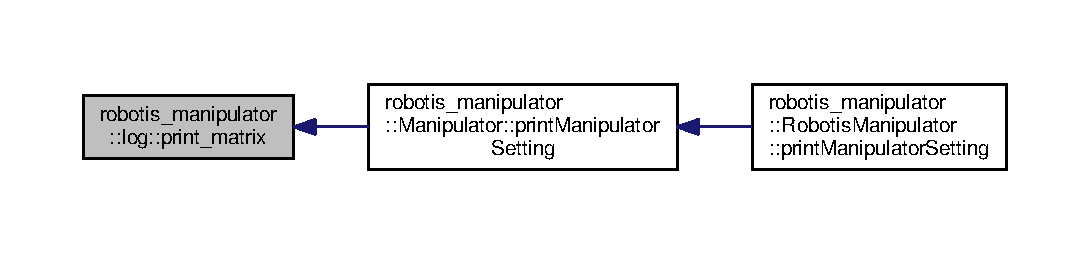
\includegraphics[width=350pt]{namespacerobotis__manipulator_1_1log_a84a7b621371c31dda949686b97b0d216_icgraph}
\end{center}
\end{figure}


\index{robotis\+\_\+manipulator\+::log@{robotis\+\_\+manipulator\+::log}!print\+\_\+vector@{print\+\_\+vector}}
\index{print\+\_\+vector@{print\+\_\+vector}!robotis\+\_\+manipulator\+::log@{robotis\+\_\+manipulator\+::log}}
\subsubsection[{\texorpdfstring{print\+\_\+vector(std\+::vector$<$ T $>$ \&vec, uint8\+\_\+t decimal\+\_\+point=3)}{print_vector(std::vector< T > &vec, uint8_t decimal_point=3)}}]{\setlength{\rightskip}{0pt plus 5cm}template$<$typename T $>$ void robotis\+\_\+manipulator\+::log\+::print\+\_\+vector (
\begin{DoxyParamCaption}
\item[{std\+::vector$<$ T $>$ \&}]{vec, }
\item[{uint8\+\_\+t}]{decimal\+\_\+point = {\ttfamily 3}}
\end{DoxyParamCaption}
)}\hypertarget{namespacerobotis__manipulator_1_1log_ab016bbac8ea97650fc14bd1be2ccdec5}{}\label{namespacerobotis__manipulator_1_1log_ab016bbac8ea97650fc14bd1be2ccdec5}


print\+\_\+vector 


\begin{DoxyParams}{Parameters}
{\em vec} & \\
\hline
{\em decimal\+\_\+point} & \\
\hline
\end{DoxyParams}


Definition at line 196 of file robotis\+\_\+manipulator\+\_\+log.\+h.


\begin{DoxyCode}
197   \{
198 \textcolor{preprocessor}{  #if defined(\_\_OPENCR\_\_)}
199     DEBUG.print(\textcolor{stringliteral}{"("});
200     \textcolor{keywordflow}{for} (uint8\_t i = 0; i < vec.size(); i++)
201     \{
202       DEBUG.print(vec.at(i), decimal\_point);
203       \textcolor{keywordflow}{if}(i != vec.size()-1)
204         DEBUG.print(\textcolor{stringliteral}{", "});
205       \textcolor{keywordflow}{else}
206         DEBUG.println(\textcolor{stringliteral}{")"});
207     \}
208 \textcolor{preprocessor}{  #else}
209     printf(\textcolor{stringliteral}{"("});
210     \textcolor{keywordflow}{for} (uint8\_t i = 0; i < vec.size(); i++)
211     \{
212       printf(\textcolor{stringliteral}{"%.*lf"}, decimal\_point, vec.at(i));
213       \textcolor{keywordflow}{if}(i != vec.size()-1)
214         printf(\textcolor{stringliteral}{", "});
215       \textcolor{keywordflow}{else}
216         printf(\textcolor{stringliteral}{")\(\backslash\)n"});
217     \}
218 \textcolor{preprocessor}{  #endif}
219   \}
\end{DoxyCode}


Here is the caller graph for this function\+:\nopagebreak
\begin{figure}[H]
\begin{center}
\leavevmode
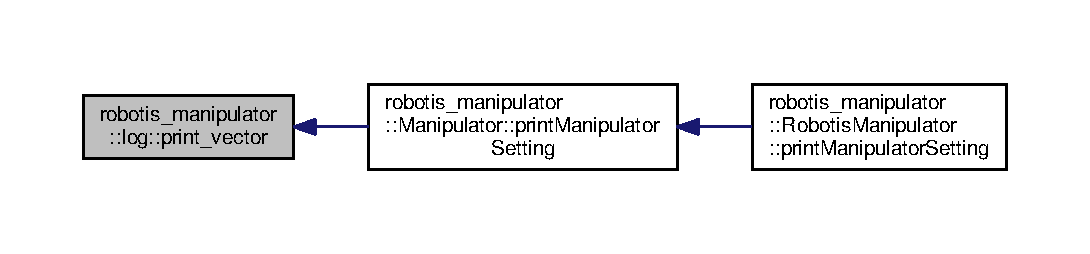
\includegraphics[width=350pt]{namespacerobotis__manipulator_1_1log_ab016bbac8ea97650fc14bd1be2ccdec5_icgraph}
\end{center}
\end{figure}


\index{robotis\+\_\+manipulator\+::log@{robotis\+\_\+manipulator\+::log}!print\+\_\+vector@{print\+\_\+vector}}
\index{print\+\_\+vector@{print\+\_\+vector}!robotis\+\_\+manipulator\+::log@{robotis\+\_\+manipulator\+::log}}
\subsubsection[{\texorpdfstring{print\+\_\+vector(vector \&vec, uint8\+\_\+t decimal\+\_\+point=3)}{print_vector(vector &vec, uint8_t decimal_point=3)}}]{\setlength{\rightskip}{0pt plus 5cm}template$<$typename vector $>$ void robotis\+\_\+manipulator\+::log\+::print\+\_\+vector (
\begin{DoxyParamCaption}
\item[{vector \&}]{vec, }
\item[{uint8\+\_\+t}]{decimal\+\_\+point = {\ttfamily 3}}
\end{DoxyParamCaption}
)}\hypertarget{namespacerobotis__manipulator_1_1log_a389a6cffbc5d0fad712e0eac8507a2ec}{}\label{namespacerobotis__manipulator_1_1log_a389a6cffbc5d0fad712e0eac8507a2ec}


print\+\_\+vector 


\begin{DoxyParams}{Parameters}
{\em vec} & \\
\hline
{\em decimal\+\_\+point} & \\
\hline
\end{DoxyParams}


Definition at line 226 of file robotis\+\_\+manipulator\+\_\+log.\+h.


\begin{DoxyCode}
227   \{
228 \textcolor{preprocessor}{  #if defined(\_\_OPENCR\_\_)}
229     DEBUG.print(\textcolor{stringliteral}{"("});
230     \textcolor{keywordflow}{for} (uint8\_t i = 0; i < vec.size(); i++)
231     \{
232       DEBUG.print(vec(i), decimal\_point);
233       \textcolor{keywordflow}{if}(i != vec.size()-1)
234         DEBUG.print(\textcolor{stringliteral}{", "});
235       \textcolor{keywordflow}{else}
236         DEBUG.println(\textcolor{stringliteral}{")"});
237     \}
238 \textcolor{preprocessor}{  #else}
239     printf(\textcolor{stringliteral}{"("});
240     \textcolor{keywordflow}{for} (uint8\_t i = 0; i < vec.size(); i++)
241     \{
242       printf(\textcolor{stringliteral}{"%.*lf"}, decimal\_point, vec(i));
243       \textcolor{keywordflow}{if}(i != vec.size()-1)
244         printf(\textcolor{stringliteral}{", "});
245       \textcolor{keywordflow}{else}
246         printf(\textcolor{stringliteral}{")\(\backslash\)n"});
247     \}
248 \textcolor{preprocessor}{  #endif}
249   \}
\end{DoxyCode}
\index{robotis\+\_\+manipulator\+::log@{robotis\+\_\+manipulator\+::log}!println@{println}}
\index{println@{println}!robotis\+\_\+manipulator\+::log@{robotis\+\_\+manipulator\+::log}}
\subsubsection[{\texorpdfstring{println(\+S\+T\+R\+I\+N\+G str, S\+T\+R\+I\+N\+G color=""D\+E\+F\+A\+U\+LT"")}{println(STRING str, STRING color="DEFAULT")}}]{\setlength{\rightskip}{0pt plus 5cm}void robotis\+\_\+manipulator\+::log\+::println (
\begin{DoxyParamCaption}
\item[{{\bf S\+T\+R\+I\+NG}}]{str, }
\item[{{\bf S\+T\+R\+I\+NG}}]{color = {\ttfamily \char`\"{}DEFAULT\char`\"{}}}
\end{DoxyParamCaption}
)}\hypertarget{namespacerobotis__manipulator_1_1log_a4a6b5b7c361aa2c61631d2c2fcfdf065}{}\label{namespacerobotis__manipulator_1_1log_a4a6b5b7c361aa2c61631d2c2fcfdf065}


println 


\begin{DoxyParams}{Parameters}
{\em str} & \\
\hline
{\em color} & \\
\hline
\end{DoxyParams}


Definition at line 92 of file robotis\+\_\+manipulator\+\_\+log.\+cpp.


\begin{DoxyCode}
93 \{
94 \textcolor{preprocessor}{#if defined(\_\_OPENCR\_\_)}
95   DEBUG.println(str);
96 \textcolor{preprocessor}{#else}
97        \textcolor{keywordflow}{if}(color == \textcolor{stringliteral}{"RED"})      printf(\hyperlink{robotis__manipulator__log_8h_a34995b955465f6bbb37c359173d50477}{ANSI\_COLOR\_RED});
98   \textcolor{keywordflow}{else} \textcolor{keywordflow}{if}(color == \textcolor{stringliteral}{"GREEN"})    printf(\hyperlink{robotis__manipulator__log_8h_a966c72d8d733c7734c6c784753d894c7}{ANSI\_COLOR\_GREEN});
99   \textcolor{keywordflow}{else} \textcolor{keywordflow}{if}(color == \textcolor{stringliteral}{"YELLOW"})   printf(\hyperlink{robotis__manipulator__log_8h_a5a123b382640b3aa65dd5db386002fbc}{ANSI\_COLOR\_YELLOW});
100   \textcolor{keywordflow}{else} \textcolor{keywordflow}{if}(color == \textcolor{stringliteral}{"BLUE"})     printf(\hyperlink{robotis__manipulator__log_8h_aca16e6a49eb51333c5fd3eee19487315}{ANSI\_COLOR\_BLUE});
101   \textcolor{keywordflow}{else} \textcolor{keywordflow}{if}(color == \textcolor{stringliteral}{"MAGENTA"})  printf(\hyperlink{robotis__manipulator__log_8h_acb30614ba1535da5b9d0c490b3c10515}{ANSI\_COLOR\_MAGENTA});
102   \textcolor{keywordflow}{else} \textcolor{keywordflow}{if}(color == \textcolor{stringliteral}{"CYAN"})     printf(\hyperlink{robotis__manipulator__log_8h_a8d0b0043e152438bb39b918a1f98c65f}{ANSI\_COLOR\_CYAN});
103   printf(\textcolor{stringliteral}{"%s\(\backslash\)n"}, str.c\_str());
104   printf(\hyperlink{robotis__manipulator__log_8h_a92a364c2b863dde1a024a77eac2a5b3b}{ANSI\_COLOR\_RESET});
105 \textcolor{preprocessor}{#endif}
106 \}
\end{DoxyCode}


Here is the caller graph for this function\+:\nopagebreak
\begin{figure}[H]
\begin{center}
\leavevmode
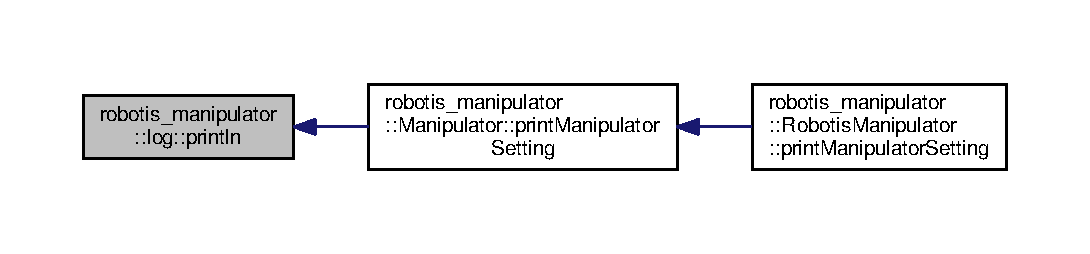
\includegraphics[width=350pt]{namespacerobotis__manipulator_1_1log_a4a6b5b7c361aa2c61631d2c2fcfdf065_icgraph}
\end{center}
\end{figure}


\index{robotis\+\_\+manipulator\+::log@{robotis\+\_\+manipulator\+::log}!println@{println}}
\index{println@{println}!robotis\+\_\+manipulator\+::log@{robotis\+\_\+manipulator\+::log}}
\subsubsection[{\texorpdfstring{println(\+S\+T\+R\+I\+N\+G str, double data, uint8\+\_\+t decimal\+\_\+point=3, S\+T\+R\+I\+N\+G color=""D\+E\+F\+A\+U\+LT"")}{println(STRING str, double data, uint8_t decimal_point=3, STRING color="DEFAULT")}}]{\setlength{\rightskip}{0pt plus 5cm}void robotis\+\_\+manipulator\+::log\+::println (
\begin{DoxyParamCaption}
\item[{{\bf S\+T\+R\+I\+NG}}]{str, }
\item[{double}]{data, }
\item[{uint8\+\_\+t}]{decimal\+\_\+point = {\ttfamily 3}, }
\item[{{\bf S\+T\+R\+I\+NG}}]{color = {\ttfamily \char`\"{}DEFAULT\char`\"{}}}
\end{DoxyParamCaption}
)}\hypertarget{namespacerobotis__manipulator_1_1log_a9e7dea27daabd2ac128133832a7e8db8}{}\label{namespacerobotis__manipulator_1_1log_a9e7dea27daabd2ac128133832a7e8db8}


println 


\begin{DoxyParams}{Parameters}
{\em str} & \\
\hline
{\em data} & \\
\hline
{\em decimal\+\_\+point} & \\
\hline
{\em color} & \\
\hline
\end{DoxyParams}


Definition at line 107 of file robotis\+\_\+manipulator\+\_\+log.\+cpp.


\begin{DoxyCode}
108 \{
109 \textcolor{preprocessor}{#if defined(\_\_OPENCR\_\_)}
110   DEBUG.print(str);
111   DEBUG.println(data, decimal\_point);
112 \textcolor{preprocessor}{#else}
113      \textcolor{keywordflow}{if}(color == \textcolor{stringliteral}{"RED"})      printf(\hyperlink{robotis__manipulator__log_8h_a34995b955465f6bbb37c359173d50477}{ANSI\_COLOR\_RED});
114   \textcolor{keywordflow}{else} \textcolor{keywordflow}{if}(color == \textcolor{stringliteral}{"GREEN"})    printf(\hyperlink{robotis__manipulator__log_8h_a966c72d8d733c7734c6c784753d894c7}{ANSI\_COLOR\_GREEN});
115   \textcolor{keywordflow}{else} \textcolor{keywordflow}{if}(color == \textcolor{stringliteral}{"YELLOW"})   printf(\hyperlink{robotis__manipulator__log_8h_a5a123b382640b3aa65dd5db386002fbc}{ANSI\_COLOR\_YELLOW});
116   \textcolor{keywordflow}{else} \textcolor{keywordflow}{if}(color == \textcolor{stringliteral}{"BLUE"})     printf(\hyperlink{robotis__manipulator__log_8h_aca16e6a49eb51333c5fd3eee19487315}{ANSI\_COLOR\_BLUE});
117   \textcolor{keywordflow}{else} \textcolor{keywordflow}{if}(color == \textcolor{stringliteral}{"MAGENTA"})  printf(\hyperlink{robotis__manipulator__log_8h_acb30614ba1535da5b9d0c490b3c10515}{ANSI\_COLOR\_MAGENTA});
118   \textcolor{keywordflow}{else} \textcolor{keywordflow}{if}(color == \textcolor{stringliteral}{"CYAN"})     printf(\hyperlink{robotis__manipulator__log_8h_a8d0b0043e152438bb39b918a1f98c65f}{ANSI\_COLOR\_CYAN});
119   printf(\textcolor{stringliteral}{"%s %.*lf\(\backslash\)n"}, str.c\_str(), decimal\_point, data);
120   printf(\hyperlink{robotis__manipulator__log_8h_a92a364c2b863dde1a024a77eac2a5b3b}{ANSI\_COLOR\_RESET});
121 \textcolor{preprocessor}{#endif}
122 \}
\end{DoxyCode}
\index{robotis\+\_\+manipulator\+::log@{robotis\+\_\+manipulator\+::log}!println@{println}}
\index{println@{println}!robotis\+\_\+manipulator\+::log@{robotis\+\_\+manipulator\+::log}}
\subsubsection[{\texorpdfstring{println(const char $\ast$str, S\+T\+R\+I\+N\+G color=""D\+E\+F\+A\+U\+LT"")}{println(const char *str, STRING color="DEFAULT")}}]{\setlength{\rightskip}{0pt plus 5cm}void robotis\+\_\+manipulator\+::log\+::println (
\begin{DoxyParamCaption}
\item[{const char $\ast$}]{str, }
\item[{{\bf S\+T\+R\+I\+NG}}]{color = {\ttfamily \char`\"{}DEFAULT\char`\"{}}}
\end{DoxyParamCaption}
)}\hypertarget{namespacerobotis__manipulator_1_1log_a950fa4b4f6a187c52e5d0721c1be551c}{}\label{namespacerobotis__manipulator_1_1log_a950fa4b4f6a187c52e5d0721c1be551c}


println 


\begin{DoxyParams}{Parameters}
{\em str} & \\
\hline
{\em color} & \\
\hline
\end{DoxyParams}


Definition at line 123 of file robotis\+\_\+manipulator\+\_\+log.\+cpp.


\begin{DoxyCode}
124 \{
125 \textcolor{preprocessor}{#if defined(\_\_OPENCR\_\_)}
126   DEBUG.println(str);
127 \textcolor{preprocessor}{#else}
128        \textcolor{keywordflow}{if}(color == \textcolor{stringliteral}{"RED"})      printf(\hyperlink{robotis__manipulator__log_8h_a34995b955465f6bbb37c359173d50477}{ANSI\_COLOR\_RED});
129   \textcolor{keywordflow}{else} \textcolor{keywordflow}{if}(color == \textcolor{stringliteral}{"GREEN"})    printf(\hyperlink{robotis__manipulator__log_8h_a966c72d8d733c7734c6c784753d894c7}{ANSI\_COLOR\_GREEN});
130   \textcolor{keywordflow}{else} \textcolor{keywordflow}{if}(color == \textcolor{stringliteral}{"YELLOW"})   printf(\hyperlink{robotis__manipulator__log_8h_a5a123b382640b3aa65dd5db386002fbc}{ANSI\_COLOR\_YELLOW});
131   \textcolor{keywordflow}{else} \textcolor{keywordflow}{if}(color == \textcolor{stringliteral}{"BLUE"})     printf(\hyperlink{robotis__manipulator__log_8h_aca16e6a49eb51333c5fd3eee19487315}{ANSI\_COLOR\_BLUE});
132   \textcolor{keywordflow}{else} \textcolor{keywordflow}{if}(color == \textcolor{stringliteral}{"MAGENTA"})  printf(\hyperlink{robotis__manipulator__log_8h_acb30614ba1535da5b9d0c490b3c10515}{ANSI\_COLOR\_MAGENTA});
133   \textcolor{keywordflow}{else} \textcolor{keywordflow}{if}(color == \textcolor{stringliteral}{"CYAN"})     printf(\hyperlink{robotis__manipulator__log_8h_a8d0b0043e152438bb39b918a1f98c65f}{ANSI\_COLOR\_CYAN});
134   printf(\textcolor{stringliteral}{"%s\(\backslash\)n"}, str);
135   printf(\hyperlink{robotis__manipulator__log_8h_a92a364c2b863dde1a024a77eac2a5b3b}{ANSI\_COLOR\_RESET});
136 \textcolor{preprocessor}{#endif}
137 \}
\end{DoxyCode}
\index{robotis\+\_\+manipulator\+::log@{robotis\+\_\+manipulator\+::log}!println@{println}}
\index{println@{println}!robotis\+\_\+manipulator\+::log@{robotis\+\_\+manipulator\+::log}}
\subsubsection[{\texorpdfstring{println(const char $\ast$str, double data, uint8\+\_\+t decimal\+\_\+point=3, S\+T\+R\+I\+N\+G color=""D\+E\+F\+A\+U\+LT"")}{println(const char *str, double data, uint8_t decimal_point=3, STRING color="DEFAULT")}}]{\setlength{\rightskip}{0pt plus 5cm}void robotis\+\_\+manipulator\+::log\+::println (
\begin{DoxyParamCaption}
\item[{const char $\ast$}]{str, }
\item[{double}]{data, }
\item[{uint8\+\_\+t}]{decimal\+\_\+point = {\ttfamily 3}, }
\item[{{\bf S\+T\+R\+I\+NG}}]{color = {\ttfamily \char`\"{}DEFAULT\char`\"{}}}
\end{DoxyParamCaption}
)}\hypertarget{namespacerobotis__manipulator_1_1log_a9582bb9bfbc4a4695975ed9e3320e3a0}{}\label{namespacerobotis__manipulator_1_1log_a9582bb9bfbc4a4695975ed9e3320e3a0}


println 


\begin{DoxyParams}{Parameters}
{\em str} & \\
\hline
{\em data} & \\
\hline
{\em decimal\+\_\+point} & \\
\hline
{\em color} & \\
\hline
\end{DoxyParams}


Definition at line 138 of file robotis\+\_\+manipulator\+\_\+log.\+cpp.


\begin{DoxyCode}
139 \{
140 \textcolor{preprocessor}{#if defined(\_\_OPENCR\_\_)}
141   DEBUG.print(str);
142   DEBUG.println(data, decimal\_point);
143 \textcolor{preprocessor}{#else}
144        \textcolor{keywordflow}{if}(color == \textcolor{stringliteral}{"RED"})      printf(\hyperlink{robotis__manipulator__log_8h_a34995b955465f6bbb37c359173d50477}{ANSI\_COLOR\_RED});
145   \textcolor{keywordflow}{else} \textcolor{keywordflow}{if}(color == \textcolor{stringliteral}{"GREEN"})    printf(\hyperlink{robotis__manipulator__log_8h_a966c72d8d733c7734c6c784753d894c7}{ANSI\_COLOR\_GREEN});
146   \textcolor{keywordflow}{else} \textcolor{keywordflow}{if}(color == \textcolor{stringliteral}{"YELLOW"})   printf(\hyperlink{robotis__manipulator__log_8h_a5a123b382640b3aa65dd5db386002fbc}{ANSI\_COLOR\_YELLOW});
147   \textcolor{keywordflow}{else} \textcolor{keywordflow}{if}(color == \textcolor{stringliteral}{"BLUE"})     printf(\hyperlink{robotis__manipulator__log_8h_aca16e6a49eb51333c5fd3eee19487315}{ANSI\_COLOR\_BLUE});
148   \textcolor{keywordflow}{else} \textcolor{keywordflow}{if}(color == \textcolor{stringliteral}{"MAGENTA"})  printf(\hyperlink{robotis__manipulator__log_8h_acb30614ba1535da5b9d0c490b3c10515}{ANSI\_COLOR\_MAGENTA});
149   \textcolor{keywordflow}{else} \textcolor{keywordflow}{if}(color == \textcolor{stringliteral}{"CYAN"})     printf(\hyperlink{robotis__manipulator__log_8h_a8d0b0043e152438bb39b918a1f98c65f}{ANSI\_COLOR\_CYAN});
150   printf(\textcolor{stringliteral}{"%s %.*lf\(\backslash\)n"}, str, decimal\_point, data);
151   printf(\hyperlink{robotis__manipulator__log_8h_a92a364c2b863dde1a024a77eac2a5b3b}{ANSI\_COLOR\_RESET});
152 \textcolor{preprocessor}{#endif}
153 \}
\end{DoxyCode}
\index{robotis\+\_\+manipulator\+::log@{robotis\+\_\+manipulator\+::log}!warn@{warn}}
\index{warn@{warn}!robotis\+\_\+manipulator\+::log@{robotis\+\_\+manipulator\+::log}}
\subsubsection[{\texorpdfstring{warn(\+S\+T\+R\+I\+N\+G str)}{warn(STRING str)}}]{\setlength{\rightskip}{0pt plus 5cm}void robotis\+\_\+manipulator\+::log\+::warn (
\begin{DoxyParamCaption}
\item[{{\bf S\+T\+R\+I\+NG}}]{str}
\end{DoxyParamCaption}
)}\hypertarget{namespacerobotis__manipulator_1_1log_a0b7fa98d31c1beaf1c7d0989723a5fa2}{}\label{namespacerobotis__manipulator_1_1log_a0b7fa98d31c1beaf1c7d0989723a5fa2}


warn 


\begin{DoxyParams}{Parameters}
{\em str} & \\
\hline
\end{DoxyParams}


Definition at line 193 of file robotis\+\_\+manipulator\+\_\+log.\+cpp.


\begin{DoxyCode}
194 \{
195 \textcolor{preprocessor}{#if defined(\_\_OPENCR\_\_)}
196   DEBUG.print(\textcolor{stringliteral}{"[WARN] "});
197   DEBUG.println(str);
198 \textcolor{preprocessor}{#else}
199   printf(\hyperlink{robotis__manipulator__log_8h_a5a123b382640b3aa65dd5db386002fbc}{ANSI\_COLOR\_YELLOW});
200   printf(\textcolor{stringliteral}{"[WARN] %s\(\backslash\)n"}, str.c\_str());
201   printf(\hyperlink{robotis__manipulator__log_8h_a92a364c2b863dde1a024a77eac2a5b3b}{ANSI\_COLOR\_RESET});
202 \textcolor{preprocessor}{#endif}
203 \}
\end{DoxyCode}
\index{robotis\+\_\+manipulator\+::log@{robotis\+\_\+manipulator\+::log}!warn@{warn}}
\index{warn@{warn}!robotis\+\_\+manipulator\+::log@{robotis\+\_\+manipulator\+::log}}
\subsubsection[{\texorpdfstring{warn(\+S\+T\+R\+I\+N\+G str, double data, uint8\+\_\+t decimal\+\_\+point=3)}{warn(STRING str, double data, uint8_t decimal_point=3)}}]{\setlength{\rightskip}{0pt plus 5cm}void robotis\+\_\+manipulator\+::log\+::warn (
\begin{DoxyParamCaption}
\item[{{\bf S\+T\+R\+I\+NG}}]{str, }
\item[{double}]{data, }
\item[{uint8\+\_\+t}]{decimal\+\_\+point = {\ttfamily 3}}
\end{DoxyParamCaption}
)}\hypertarget{namespacerobotis__manipulator_1_1log_aac4f8d437de82deb67e7e9c4688dfcdc}{}\label{namespacerobotis__manipulator_1_1log_aac4f8d437de82deb67e7e9c4688dfcdc}


warn 


\begin{DoxyParams}{Parameters}
{\em str} & \\
\hline
{\em data} & \\
\hline
{\em decimal\+\_\+point} & \\
\hline
\end{DoxyParams}


Definition at line 204 of file robotis\+\_\+manipulator\+\_\+log.\+cpp.


\begin{DoxyCode}
205 \{
206 \textcolor{preprocessor}{#if defined(\_\_OPENCR\_\_)}
207   DEBUG.print(\textcolor{stringliteral}{"[WARN] "});
208   DEBUG.print(str);
209   DEBUG.println(data, decimal\_point);
210 \textcolor{preprocessor}{#else}
211   printf(\hyperlink{robotis__manipulator__log_8h_a5a123b382640b3aa65dd5db386002fbc}{ANSI\_COLOR\_YELLOW});
212   printf(\textcolor{stringliteral}{"[WARN] %s %.*lf\(\backslash\)n"},str.c\_str(), decimal\_point, data);
213   printf(\hyperlink{robotis__manipulator__log_8h_a92a364c2b863dde1a024a77eac2a5b3b}{ANSI\_COLOR\_RESET});
214 \textcolor{preprocessor}{#endif}
215 \}
\end{DoxyCode}
\index{robotis\+\_\+manipulator\+::log@{robotis\+\_\+manipulator\+::log}!warn@{warn}}
\index{warn@{warn}!robotis\+\_\+manipulator\+::log@{robotis\+\_\+manipulator\+::log}}
\subsubsection[{\texorpdfstring{warn(const char $\ast$str)}{warn(const char *str)}}]{\setlength{\rightskip}{0pt plus 5cm}void robotis\+\_\+manipulator\+::log\+::warn (
\begin{DoxyParamCaption}
\item[{const char $\ast$}]{str}
\end{DoxyParamCaption}
)}\hypertarget{namespacerobotis__manipulator_1_1log_adcfad83d39b25e03a57b8cb20283606b}{}\label{namespacerobotis__manipulator_1_1log_adcfad83d39b25e03a57b8cb20283606b}


warn 


\begin{DoxyParams}{Parameters}
{\em str} & \\
\hline
\end{DoxyParams}


Definition at line 216 of file robotis\+\_\+manipulator\+\_\+log.\+cpp.


\begin{DoxyCode}
217 \{
218 \textcolor{preprocessor}{#if defined(\_\_OPENCR\_\_)}
219   DEBUG.print(\textcolor{stringliteral}{"[WARN] "});
220   DEBUG.println(str);
221 \textcolor{preprocessor}{#else}
222   printf(\hyperlink{robotis__manipulator__log_8h_a5a123b382640b3aa65dd5db386002fbc}{ANSI\_COLOR\_YELLOW});
223   printf(\textcolor{stringliteral}{"[WARN] %s\(\backslash\)n"}, str);
224   printf(\hyperlink{robotis__manipulator__log_8h_a92a364c2b863dde1a024a77eac2a5b3b}{ANSI\_COLOR\_RESET});
225 \textcolor{preprocessor}{#endif}
226 \}
\end{DoxyCode}
\index{robotis\+\_\+manipulator\+::log@{robotis\+\_\+manipulator\+::log}!warn@{warn}}
\index{warn@{warn}!robotis\+\_\+manipulator\+::log@{robotis\+\_\+manipulator\+::log}}
\subsubsection[{\texorpdfstring{warn(const char $\ast$str, double data, uint8\+\_\+t decimal\+\_\+point=3)}{warn(const char *str, double data, uint8_t decimal_point=3)}}]{\setlength{\rightskip}{0pt plus 5cm}void robotis\+\_\+manipulator\+::log\+::warn (
\begin{DoxyParamCaption}
\item[{const char $\ast$}]{str, }
\item[{double}]{data, }
\item[{uint8\+\_\+t}]{decimal\+\_\+point = {\ttfamily 3}}
\end{DoxyParamCaption}
)}\hypertarget{namespacerobotis__manipulator_1_1log_a6b4909ba686cc8ca3f5e4ee9b3eb5ec1}{}\label{namespacerobotis__manipulator_1_1log_a6b4909ba686cc8ca3f5e4ee9b3eb5ec1}


warn 


\begin{DoxyParams}{Parameters}
{\em str} & \\
\hline
{\em data} & \\
\hline
{\em decimal\+\_\+point} & \\
\hline
\end{DoxyParams}


Definition at line 227 of file robotis\+\_\+manipulator\+\_\+log.\+cpp.


\begin{DoxyCode}
228 \{
229 \textcolor{preprocessor}{#if defined(\_\_OPENCR\_\_)}
230   DEBUG.print(\textcolor{stringliteral}{"[WARN] "});
231   DEBUG.print(str);
232   DEBUG.println(data, decimal\_point);
233 \textcolor{preprocessor}{#else}
234   printf(\hyperlink{robotis__manipulator__log_8h_a5a123b382640b3aa65dd5db386002fbc}{ANSI\_COLOR\_YELLOW});
235   printf(\textcolor{stringliteral}{"[WARN] %s %.*lf\(\backslash\)n"}, str, decimal\_point, data);
236   printf(\hyperlink{robotis__manipulator__log_8h_a92a364c2b863dde1a024a77eac2a5b3b}{ANSI\_COLOR\_RESET});
237 \textcolor{preprocessor}{#endif}
238 \}
\end{DoxyCode}

\hypertarget{namespacerobotis__manipulator_1_1math}{}\section{robotis\+\_\+manipulator\+:\+:math Namespace Reference}
\label{namespacerobotis__manipulator_1_1math}\index{robotis\+\_\+manipulator\+::math@{robotis\+\_\+manipulator\+::math}}
\subsection*{Functions}
\begin{DoxyCompactItemize}
\item 
Eigen\+::\+Vector3d \hyperlink{namespacerobotis__manipulator_1_1math_a057ca65131575b85aec169f3a50ed796}{vector3} (double v1, double v2, double v3)
\begin{DoxyCompactList}\small\item\em vector3 \end{DoxyCompactList}\item 
Eigen\+::\+Matrix3d \hyperlink{namespacerobotis__manipulator_1_1math_a22fb2daaef2f7943fa0dbd7a24e0fd4d}{matrix3} (double m11, double m12, double m13, double m21, double m22, double m23, double m31, double m32, double m33)
\begin{DoxyCompactList}\small\item\em matrix3 \end{DoxyCompactList}\item 
Eigen\+::\+Matrix3d \hyperlink{namespacerobotis__manipulator_1_1math_a34ebf1c9f0f64e52807fd9798a7d87c8}{inertia\+Matrix} (double ixx, double ixy, double ixz, double iyy, double iyz, double izz)
\begin{DoxyCompactList}\small\item\em inertia\+Matrix \end{DoxyCompactList}\item 
Eigen\+::\+Vector3d \hyperlink{namespacerobotis__manipulator_1_1math_acb3c85751c21502d8d23a13cc08b3cf5}{convert\+X\+Y\+Z\+To\+Vector} (double x, double y, double z)
\begin{DoxyCompactList}\small\item\em convert\+X\+Y\+Z\+To\+Vector \end{DoxyCompactList}\item 
Eigen\+::\+Matrix3d \hyperlink{namespacerobotis__manipulator_1_1math_ab7682932090e254cb077badb80fe8667}{convert\+Roll\+Angle\+To\+Rotation\+Matrix} (double angle)
\begin{DoxyCompactList}\small\item\em convert\+Roll\+Angle\+To\+Rotation\+Matrix \end{DoxyCompactList}\item 
Eigen\+::\+Matrix3d \hyperlink{namespacerobotis__manipulator_1_1math_aa6112f12db3755d6677f45c9e0806cbf}{convert\+Pitch\+Angle\+To\+Rotation\+Matrix} (double angle)
\begin{DoxyCompactList}\small\item\em convert\+Pitch\+Angle\+To\+Rotation\+Matrix \end{DoxyCompactList}\item 
Eigen\+::\+Matrix3d \hyperlink{namespacerobotis__manipulator_1_1math_a0a45b10176c2a214876aa265ec8e707e}{convert\+Yaw\+Angle\+To\+Rotation\+Matrix} (double angle)
\begin{DoxyCompactList}\small\item\em convert\+Yaw\+Angle\+To\+Rotation\+Matrix \end{DoxyCompactList}\item 
Eigen\+::\+Vector3d \hyperlink{namespacerobotis__manipulator_1_1math_adaa070908c6328c2459be5eaf64af68f}{convert\+Rotation\+Matrix\+To\+R\+P\+Y\+Vector} (const Eigen\+::\+Matrix3d \&rotation\+\_\+matrix)
\begin{DoxyCompactList}\small\item\em convert\+Rotation\+Matrix\+To\+R\+P\+Y\+Vector \end{DoxyCompactList}\item 
Eigen\+::\+Matrix3d \hyperlink{namespacerobotis__manipulator_1_1math_a4bbc795e8c06dd0472ed25864f6ec886}{convert\+R\+P\+Y\+To\+Rotation\+Matrix} (double roll, double pitch, double yaw)
\begin{DoxyCompactList}\small\item\em convert\+R\+P\+Y\+To\+Rotation\+Matrix \end{DoxyCompactList}\item 
Eigen\+::\+Quaterniond \hyperlink{namespacerobotis__manipulator_1_1math_aa1d5ec03193d986594c03ab884126416}{convert\+R\+P\+Y\+To\+Quaternion} (double roll, double pitch, double yaw)
\begin{DoxyCompactList}\small\item\em convert\+R\+P\+Y\+To\+Quaternion \end{DoxyCompactList}\item 
Eigen\+::\+Quaterniond \hyperlink{namespacerobotis__manipulator_1_1math_ae5a4fd98d1cef4a4b1224b19daff63bf}{convert\+Rotation\+Matrix\+To\+Quaternion} (const Eigen\+::\+Matrix3d \&rotation\+\_\+matrix)
\begin{DoxyCompactList}\small\item\em convert\+Rotation\+Matrix\+To\+Quaternion \end{DoxyCompactList}\item 
Eigen\+::\+Vector3d \hyperlink{namespacerobotis__manipulator_1_1math_a5d6107f6a65d430f3eee81f93327c37a}{convert\+Quaternion\+To\+R\+P\+Y\+Vector} (const Eigen\+::\+Quaterniond \&quaternion)
\begin{DoxyCompactList}\small\item\em convert\+Quaternion\+To\+R\+P\+Y\+Vector \end{DoxyCompactList}\item 
Eigen\+::\+Matrix3d \hyperlink{namespacerobotis__manipulator_1_1math_a7a7c421fe85e75a3897a4c0c492bb662}{convert\+Quaternion\+To\+Rotation\+Matrix} (const Eigen\+::\+Quaterniond \&quaternion)
\begin{DoxyCompactList}\small\item\em convert\+Quaternion\+To\+Rotation\+Matrix \end{DoxyCompactList}\item 
Eigen\+::\+Vector3d \hyperlink{namespacerobotis__manipulator_1_1math_a0659ad2d283ad43e01eca23f0be6a134}{convert\+Rotation\+Matrix\+To\+Omega} (const Eigen\+::\+Matrix3d \&rotation\+\_\+matrix)
\begin{DoxyCompactList}\small\item\em convert\+Rotation\+Matrix\+To\+Omega \end{DoxyCompactList}\item 
Eigen\+::\+Matrix4d \hyperlink{namespacerobotis__manipulator_1_1math_a5f001cf17bbf0daaaacd46f58d3f6e8a}{convert\+X\+Y\+Z\+R\+P\+Y\+To\+Transformation\+Matrix} (double x, double y, double z, double roll, double pitch, double yaw)
\begin{DoxyCompactList}\small\item\em convert\+X\+Y\+Z\+R\+P\+Y\+To\+Transformation\+Matrix \end{DoxyCompactList}\item 
Eigen\+::\+Matrix4d \hyperlink{namespacerobotis__manipulator_1_1math_a0e864bea906520574b93496db74427f0}{convert\+X\+Y\+Z\+To\+Transformation\+Matrix} (double x, double y, double z)
\begin{DoxyCompactList}\small\item\em convert\+X\+Y\+Z\+To\+Transformation\+Matrix \end{DoxyCompactList}\item 
Eigen\+::\+Matrix4d \hyperlink{namespacerobotis__manipulator_1_1math_a82a56f3cb0404e06bf37f2e167c839ef}{convert\+R\+P\+Y\+To\+Transformation\+Matrix} (double roll, double pitch, double yaw)
\begin{DoxyCompactList}\small\item\em convert\+R\+P\+Y\+To\+Transformation\+Matrix \end{DoxyCompactList}\item 
Eigen\+::\+Vector3d \hyperlink{namespacerobotis__manipulator_1_1math_ae69e1aacc48ed72442eb4dc82e280be0}{convert\+Omega\+To\+R\+P\+Y\+Velocity} (Eigen\+::\+Vector3d rpy\+\_\+vector, Eigen\+::\+Vector3d omega)
\begin{DoxyCompactList}\small\item\em convert\+Omega\+To\+R\+P\+Y\+Velocity \end{DoxyCompactList}\item 
Eigen\+::\+Vector3d \hyperlink{namespacerobotis__manipulator_1_1math_a73d50f3962eeac18f464f879e6a0c8fc}{convert\+R\+P\+Y\+Velocity\+To\+Omega} (Eigen\+::\+Vector3d rpy\+\_\+vector, Eigen\+::\+Vector3d rpy\+\_\+velocity)
\begin{DoxyCompactList}\small\item\em convert\+R\+P\+Y\+Velocity\+To\+Omega \end{DoxyCompactList}\item 
Eigen\+::\+Vector3d \hyperlink{namespacerobotis__manipulator_1_1math_aabd3cc7c059a6372e917bc98a3e5c1dd}{convert\+Omega\+Dot\+To\+R\+P\+Y\+Acceleration} (Eigen\+::\+Vector3d rpy\+\_\+vector, Eigen\+::\+Vector3d rpy\+\_\+velocity, Eigen\+::\+Vector3d omega\+\_\+dot)
\begin{DoxyCompactList}\small\item\em convert\+Omega\+Dot\+To\+R\+P\+Y\+Acceleration \end{DoxyCompactList}\item 
Eigen\+::\+Vector3d \hyperlink{namespacerobotis__manipulator_1_1math_a752d1631596538515894f09f210eb17b}{convert\+R\+P\+Y\+Acceleration\+To\+Omega\+Dot} (Eigen\+::\+Vector3d rpy\+\_\+vector, Eigen\+::\+Vector3d rpy\+\_\+velocity, Eigen\+::\+Vector3d rpy\+\_\+acceleration)
\begin{DoxyCompactList}\small\item\em convert\+R\+P\+Y\+Acceleration\+To\+Omega\+Dot \end{DoxyCompactList}\item 
double \hyperlink{namespacerobotis__manipulator_1_1math_a27a6dd481239e8377185dac85cf9cd77}{sign} (double value)
\begin{DoxyCompactList}\small\item\em sign \end{DoxyCompactList}\item 
Eigen\+::\+Matrix4d \hyperlink{namespacerobotis__manipulator_1_1math_a0e23b77220a7f83814de154838a47be7}{inverse\+Transformation\+Matrix} (const Eigen\+::\+Matrix\+Xd \&transformation\+\_\+matrix)
\begin{DoxyCompactList}\small\item\em inverse\+Transformation\+Matrix \end{DoxyCompactList}\item 
Eigen\+::\+Vector3d \hyperlink{namespacerobotis__manipulator_1_1math_a38b3c7716c5b8a29a75d8b3243eb75e7}{matrix\+Logarithm} (Eigen\+::\+Matrix3d rotation\+\_\+matrix)
\begin{DoxyCompactList}\small\item\em matrix\+Logarithm \end{DoxyCompactList}\item 
Eigen\+::\+Matrix3d \hyperlink{namespacerobotis__manipulator_1_1math_a03bf0fffc828339f2216fd4a98a32923}{skew\+Symmetric\+Matrix} (Eigen\+::\+Vector3d v)
\begin{DoxyCompactList}\small\item\em skew\+Symmetric\+Matrix \end{DoxyCompactList}\item 
Eigen\+::\+Matrix3d \hyperlink{namespacerobotis__manipulator_1_1math_a515d31a7d3b19cce814cd121717bcb60}{rodrigues\+Rotation\+Matrix} (Eigen\+::\+Vector3d axis, double angle)
\begin{DoxyCompactList}\small\item\em rodrigues\+Rotation\+Matrix \end{DoxyCompactList}\item 
Eigen\+::\+Vector3d \hyperlink{namespacerobotis__manipulator_1_1math_ab4f15d22dddddc5f712de188ba0f85f4}{position\+Difference} (Eigen\+::\+Vector3d desired\+\_\+position, Eigen\+::\+Vector3d present\+\_\+position)
\begin{DoxyCompactList}\small\item\em position\+Difference \end{DoxyCompactList}\item 
Eigen\+::\+Vector3d \hyperlink{namespacerobotis__manipulator_1_1math_a26796dad948a40bc2c0ac2c139ed85f0}{orientation\+Difference} (Eigen\+::\+Matrix3d desired\+\_\+orientation, Eigen\+::\+Matrix3d present\+\_\+orientation)
\begin{DoxyCompactList}\small\item\em orientation\+Difference \end{DoxyCompactList}\item 
Eigen\+::\+Vector\+Xd \hyperlink{namespacerobotis__manipulator_1_1math_a5bf9202c405abf15e234505842bf7361}{pose\+Difference} (Eigen\+::\+Vector3d desired\+\_\+position, Eigen\+::\+Vector3d present\+\_\+position, Eigen\+::\+Matrix3d desired\+\_\+orientation, Eigen\+::\+Matrix3d present\+\_\+orientation)
\begin{DoxyCompactList}\small\item\em pose\+Difference \end{DoxyCompactList}\end{DoxyCompactItemize}


\subsection{Function Documentation}
\index{robotis\+\_\+manipulator\+::math@{robotis\+\_\+manipulator\+::math}!convert\+Omega\+Dot\+To\+R\+P\+Y\+Acceleration@{convert\+Omega\+Dot\+To\+R\+P\+Y\+Acceleration}}
\index{convert\+Omega\+Dot\+To\+R\+P\+Y\+Acceleration@{convert\+Omega\+Dot\+To\+R\+P\+Y\+Acceleration}!robotis\+\_\+manipulator\+::math@{robotis\+\_\+manipulator\+::math}}
\subsubsection[{\texorpdfstring{convert\+Omega\+Dot\+To\+R\+P\+Y\+Acceleration(\+Eigen\+::\+Vector3d rpy\+\_\+vector, Eigen\+::\+Vector3d rpy\+\_\+velocity, Eigen\+::\+Vector3d omega\+\_\+dot)}{convertOmegaDotToRPYAcceleration(Eigen::Vector3d rpy_vector, Eigen::Vector3d rpy_velocity, Eigen::Vector3d omega_dot)}}]{\setlength{\rightskip}{0pt plus 5cm}Eigen\+::\+Vector3d robotis\+\_\+manipulator\+::math\+::convert\+Omega\+Dot\+To\+R\+P\+Y\+Acceleration (
\begin{DoxyParamCaption}
\item[{Eigen\+::\+Vector3d}]{rpy\+\_\+vector, }
\item[{Eigen\+::\+Vector3d}]{rpy\+\_\+velocity, }
\item[{Eigen\+::\+Vector3d}]{omega\+\_\+dot}
\end{DoxyParamCaption}
)}\hypertarget{namespacerobotis__manipulator_1_1math_aabd3cc7c059a6372e917bc98a3e5c1dd}{}\label{namespacerobotis__manipulator_1_1math_aabd3cc7c059a6372e917bc98a3e5c1dd}


convert\+Omega\+Dot\+To\+R\+P\+Y\+Acceleration 


\begin{DoxyParams}{Parameters}
{\em rpy\+\_\+vector} & \\
\hline
{\em rpy\+\_\+velocity} & \\
\hline
{\em omega\+\_\+dot} & \\
\hline
\end{DoxyParams}
\begin{DoxyReturn}{Returns}

\end{DoxyReturn}


Definition at line 266 of file robotis\+\_\+manipulator\+\_\+math.\+cpp.


\begin{DoxyCode}
267 \{
268   Eigen::Vector3d c\_dot;
269   Eigen::Matrix3d c\_inverse;
270   Eigen::Vector3d rpy\_acceleration;
271 
272   c\_dot << -cos(rpy\_vector[1]) * rpy\_velocity[1] * rpy\_velocity[2],
273            -sin(rpy\_vector[0]) * rpy\_velocity[0] * rpy\_velocity[1] - sin(rpy\_vector[0]) * sin(rpy\_vector[1]
      ) * rpy\_velocity[1] * rpy\_velocity[2] + cos(rpy\_vector[0]) * cos(rpy\_vector[1]) * rpy\_velocity[0] * 
      rpy\_velocity[2],
274            -cos(rpy\_vector[0]) * rpy\_velocity[0] * rpy\_velocity[1] - sin(rpy\_vector[0]) * cos(rpy\_vector[1]
      ) * rpy\_velocity[0] * rpy\_velocity[2] - cos(rpy\_vector[0]) * sin(rpy\_vector[1]) * rpy\_velocity[1] * 
      rpy\_velocity[2];
275 
276   c\_inverse << 1, sin(rpy\_vector(0))*tan(rpy\_vector(1)), cos(rpy\_vector(0))*tan(rpy\_vector(1)),
277        0, cos(rpy\_vector(0)),                    -sin(rpy\_vector(0)),
278        0, sin(rpy\_vector(0))/cos(rpy\_vector(1)), cos(rpy\_vector(0))/cos(rpy\_vector(1));
279 
280   rpy\_acceleration = c\_inverse * (omega\_dot - c\_dot);
281   \textcolor{keywordflow}{return} rpy\_acceleration;
282 \}
\end{DoxyCode}


Here is the caller graph for this function\+:\nopagebreak
\begin{figure}[H]
\begin{center}
\leavevmode
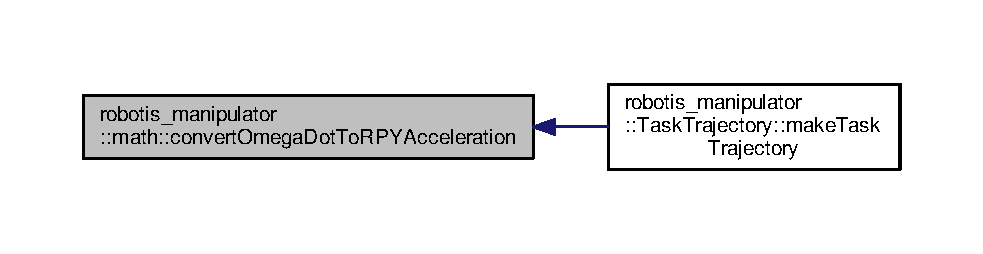
\includegraphics[width=350pt]{namespacerobotis__manipulator_1_1math_aabd3cc7c059a6372e917bc98a3e5c1dd_icgraph}
\end{center}
\end{figure}


\index{robotis\+\_\+manipulator\+::math@{robotis\+\_\+manipulator\+::math}!convert\+Omega\+To\+R\+P\+Y\+Velocity@{convert\+Omega\+To\+R\+P\+Y\+Velocity}}
\index{convert\+Omega\+To\+R\+P\+Y\+Velocity@{convert\+Omega\+To\+R\+P\+Y\+Velocity}!robotis\+\_\+manipulator\+::math@{robotis\+\_\+manipulator\+::math}}
\subsubsection[{\texorpdfstring{convert\+Omega\+To\+R\+P\+Y\+Velocity(\+Eigen\+::\+Vector3d rpy\+\_\+vector, Eigen\+::\+Vector3d omega)}{convertOmegaToRPYVelocity(Eigen::Vector3d rpy_vector, Eigen::Vector3d omega)}}]{\setlength{\rightskip}{0pt plus 5cm}Eigen\+::\+Vector3d robotis\+\_\+manipulator\+::math\+::convert\+Omega\+To\+R\+P\+Y\+Velocity (
\begin{DoxyParamCaption}
\item[{Eigen\+::\+Vector3d}]{rpy\+\_\+vector, }
\item[{Eigen\+::\+Vector3d}]{omega}
\end{DoxyParamCaption}
)}\hypertarget{namespacerobotis__manipulator_1_1math_ae69e1aacc48ed72442eb4dc82e280be0}{}\label{namespacerobotis__manipulator_1_1math_ae69e1aacc48ed72442eb4dc82e280be0}


convert\+Omega\+To\+R\+P\+Y\+Velocity 


\begin{DoxyParams}{Parameters}
{\em rpy\+\_\+vector} & \\
\hline
{\em omega} & \\
\hline
\end{DoxyParams}
\begin{DoxyReturn}{Returns}

\end{DoxyReturn}


Definition at line 240 of file robotis\+\_\+manipulator\+\_\+math.\+cpp.


\begin{DoxyCode}
241 \{
242   Eigen::Matrix3d c\_inverse;
243   Eigen::Vector3d rpy\_velocity;
244 
245   c\_inverse << 1, sin(rpy\_vector(0))*tan(rpy\_vector(1)), cos(rpy\_vector(0))*tan(rpy\_vector(1)),
246        0, cos(rpy\_vector(0)),                    -sin(rpy\_vector(0)),
247        0, sin(rpy\_vector(0))/cos(rpy\_vector(1)), cos(rpy\_vector(0))/cos(rpy\_vector(1));
248 
249   rpy\_velocity = c\_inverse * omega;
250   \textcolor{keywordflow}{return} rpy\_velocity;
251 \}
\end{DoxyCode}


Here is the caller graph for this function\+:\nopagebreak
\begin{figure}[H]
\begin{center}
\leavevmode
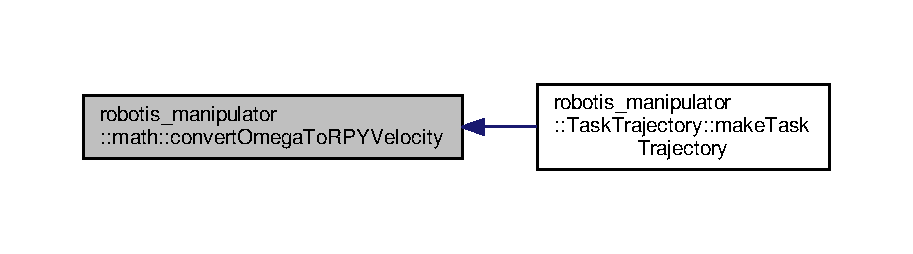
\includegraphics[width=350pt]{namespacerobotis__manipulator_1_1math_ae69e1aacc48ed72442eb4dc82e280be0_icgraph}
\end{center}
\end{figure}


\index{robotis\+\_\+manipulator\+::math@{robotis\+\_\+manipulator\+::math}!convert\+Pitch\+Angle\+To\+Rotation\+Matrix@{convert\+Pitch\+Angle\+To\+Rotation\+Matrix}}
\index{convert\+Pitch\+Angle\+To\+Rotation\+Matrix@{convert\+Pitch\+Angle\+To\+Rotation\+Matrix}!robotis\+\_\+manipulator\+::math@{robotis\+\_\+manipulator\+::math}}
\subsubsection[{\texorpdfstring{convert\+Pitch\+Angle\+To\+Rotation\+Matrix(double angle)}{convertPitchAngleToRotationMatrix(double angle)}}]{\setlength{\rightskip}{0pt plus 5cm}Eigen\+::\+Matrix3d robotis\+\_\+manipulator\+::math\+::convert\+Pitch\+Angle\+To\+Rotation\+Matrix (
\begin{DoxyParamCaption}
\item[{double}]{angle}
\end{DoxyParamCaption}
)}\hypertarget{namespacerobotis__manipulator_1_1math_aa6112f12db3755d6677f45c9e0806cbf}{}\label{namespacerobotis__manipulator_1_1math_aa6112f12db3755d6677f45c9e0806cbf}


convert\+Pitch\+Angle\+To\+Rotation\+Matrix 


\begin{DoxyParams}{Parameters}
{\em angle} & \\
\hline
\end{DoxyParams}
\begin{DoxyReturn}{Returns}

\end{DoxyReturn}


Definition at line 83 of file robotis\+\_\+manipulator\+\_\+math.\+cpp.


\begin{DoxyCode}
84 \{
85   Eigen::Matrix3d rotation(3,3);
86   rotation <<
87       cos(angle), 0.0, sin(angle),
88       0.0, 1.0, 0.0,
89       -sin(angle), 0.0, cos(angle);
90 
91   \textcolor{keywordflow}{return} rotation;
92 \}
\end{DoxyCode}


Here is the caller graph for this function\+:\nopagebreak
\begin{figure}[H]
\begin{center}
\leavevmode
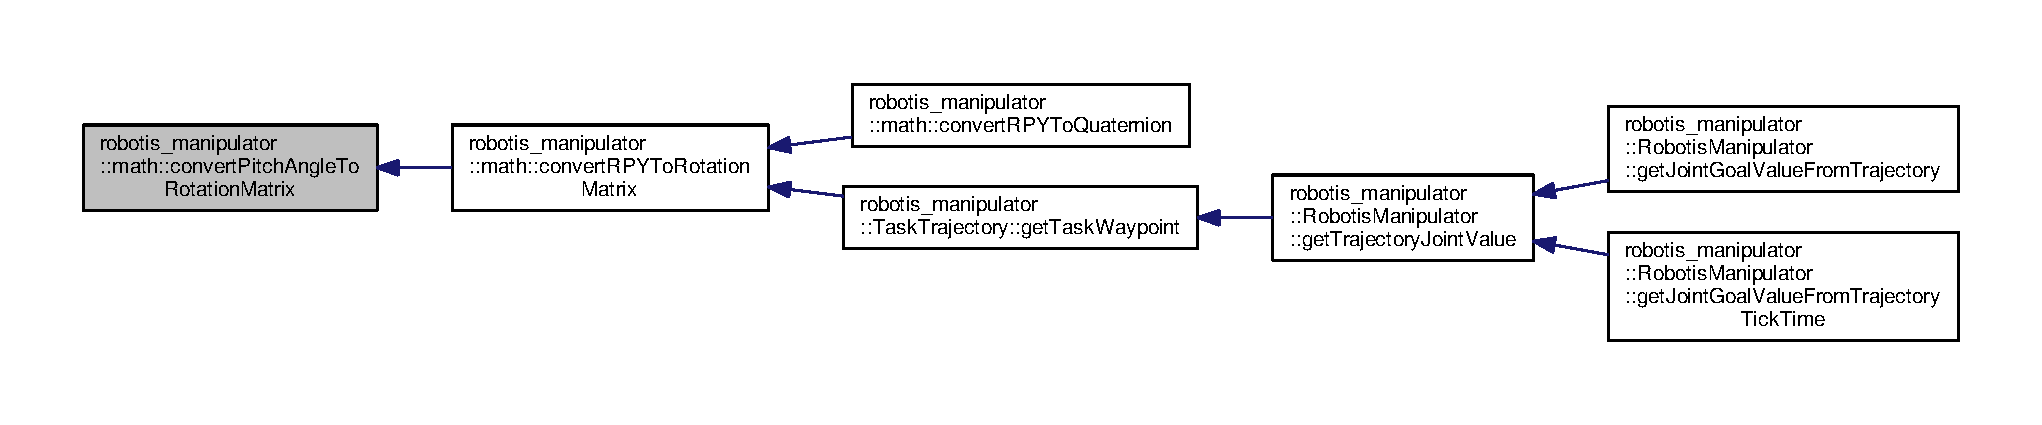
\includegraphics[width=350pt]{namespacerobotis__manipulator_1_1math_aa6112f12db3755d6677f45c9e0806cbf_icgraph}
\end{center}
\end{figure}


\index{robotis\+\_\+manipulator\+::math@{robotis\+\_\+manipulator\+::math}!convert\+Quaternion\+To\+Rotation\+Matrix@{convert\+Quaternion\+To\+Rotation\+Matrix}}
\index{convert\+Quaternion\+To\+Rotation\+Matrix@{convert\+Quaternion\+To\+Rotation\+Matrix}!robotis\+\_\+manipulator\+::math@{robotis\+\_\+manipulator\+::math}}
\subsubsection[{\texorpdfstring{convert\+Quaternion\+To\+Rotation\+Matrix(const Eigen\+::\+Quaterniond \&quaternion)}{convertQuaternionToRotationMatrix(const Eigen::Quaterniond &quaternion)}}]{\setlength{\rightskip}{0pt plus 5cm}Eigen\+::\+Matrix3d robotis\+\_\+manipulator\+::math\+::convert\+Quaternion\+To\+Rotation\+Matrix (
\begin{DoxyParamCaption}
\item[{const Eigen\+::\+Quaterniond \&}]{quaternion}
\end{DoxyParamCaption}
)}\hypertarget{namespacerobotis__manipulator_1_1math_a7a7c421fe85e75a3897a4c0c492bb662}{}\label{namespacerobotis__manipulator_1_1math_a7a7c421fe85e75a3897a4c0c492bb662}


convert\+Quaternion\+To\+Rotation\+Matrix 


\begin{DoxyParams}{Parameters}
{\em quaternion} & \\
\hline
\end{DoxyParams}
\begin{DoxyReturn}{Returns}

\end{DoxyReturn}


Definition at line 145 of file robotis\+\_\+manipulator\+\_\+math.\+cpp.


\begin{DoxyCode}
146 \{
147   Eigen::Matrix3d rotation = quaternion.toRotationMatrix();
148 
149   \textcolor{keywordflow}{return} rotation;
150 \}
\end{DoxyCode}
\index{robotis\+\_\+manipulator\+::math@{robotis\+\_\+manipulator\+::math}!convert\+Quaternion\+To\+R\+P\+Y\+Vector@{convert\+Quaternion\+To\+R\+P\+Y\+Vector}}
\index{convert\+Quaternion\+To\+R\+P\+Y\+Vector@{convert\+Quaternion\+To\+R\+P\+Y\+Vector}!robotis\+\_\+manipulator\+::math@{robotis\+\_\+manipulator\+::math}}
\subsubsection[{\texorpdfstring{convert\+Quaternion\+To\+R\+P\+Y\+Vector(const Eigen\+::\+Quaterniond \&quaternion)}{convertQuaternionToRPYVector(const Eigen::Quaterniond &quaternion)}}]{\setlength{\rightskip}{0pt plus 5cm}Eigen\+::\+Vector3d robotis\+\_\+manipulator\+::math\+::convert\+Quaternion\+To\+R\+P\+Y\+Vector (
\begin{DoxyParamCaption}
\item[{const Eigen\+::\+Quaterniond \&}]{quaternion}
\end{DoxyParamCaption}
)}\hypertarget{namespacerobotis__manipulator_1_1math_a5d6107f6a65d430f3eee81f93327c37a}{}\label{namespacerobotis__manipulator_1_1math_a5d6107f6a65d430f3eee81f93327c37a}


convert\+Quaternion\+To\+R\+P\+Y\+Vector 


\begin{DoxyParams}{Parameters}
{\em quaternion} & \\
\hline
\end{DoxyParams}
\begin{DoxyReturn}{Returns}

\end{DoxyReturn}


Definition at line 138 of file robotis\+\_\+manipulator\+\_\+math.\+cpp.


\begin{DoxyCode}
139 \{
140   Eigen::Vector3d rpy = 
      \hyperlink{namespacerobotis__manipulator_1_1math_adaa070908c6328c2459be5eaf64af68f}{robotis\_manipulator::math::convertRotationMatrixToRPYVector}
      (quaternion.toRotationMatrix());
141 
142   \textcolor{keywordflow}{return} rpy;
143 \}
\end{DoxyCode}


Here is the call graph for this function\+:\nopagebreak
\begin{figure}[H]
\begin{center}
\leavevmode
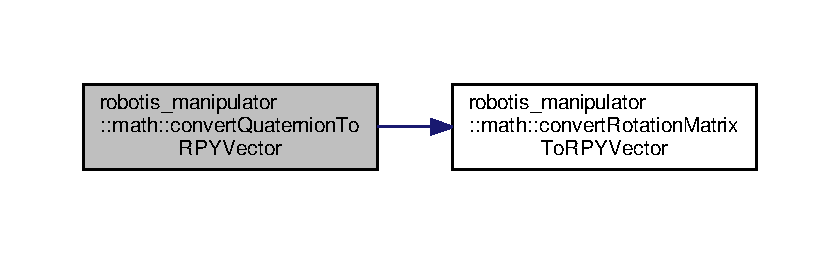
\includegraphics[width=350pt]{namespacerobotis__manipulator_1_1math_a5d6107f6a65d430f3eee81f93327c37a_cgraph}
\end{center}
\end{figure}


\index{robotis\+\_\+manipulator\+::math@{robotis\+\_\+manipulator\+::math}!convert\+Roll\+Angle\+To\+Rotation\+Matrix@{convert\+Roll\+Angle\+To\+Rotation\+Matrix}}
\index{convert\+Roll\+Angle\+To\+Rotation\+Matrix@{convert\+Roll\+Angle\+To\+Rotation\+Matrix}!robotis\+\_\+manipulator\+::math@{robotis\+\_\+manipulator\+::math}}
\subsubsection[{\texorpdfstring{convert\+Roll\+Angle\+To\+Rotation\+Matrix(double angle)}{convertRollAngleToRotationMatrix(double angle)}}]{\setlength{\rightskip}{0pt plus 5cm}Eigen\+::\+Matrix3d robotis\+\_\+manipulator\+::math\+::convert\+Roll\+Angle\+To\+Rotation\+Matrix (
\begin{DoxyParamCaption}
\item[{double}]{angle}
\end{DoxyParamCaption}
)}\hypertarget{namespacerobotis__manipulator_1_1math_ab7682932090e254cb077badb80fe8667}{}\label{namespacerobotis__manipulator_1_1math_ab7682932090e254cb077badb80fe8667}


convert\+Roll\+Angle\+To\+Rotation\+Matrix 


\begin{DoxyParams}{Parameters}
{\em angle} & \\
\hline
\end{DoxyParams}
\begin{DoxyReturn}{Returns}

\end{DoxyReturn}


Definition at line 72 of file robotis\+\_\+manipulator\+\_\+math.\+cpp.


\begin{DoxyCode}
73 \{
74   Eigen::Matrix3d rotation(3,3);
75   rotation <<
76       1.0, 0.0, 0.0,
77       0.0, cos(angle), -sin(angle),
78       0.0, sin(angle), cos(angle);
79 
80   \textcolor{keywordflow}{return} rotation;
81 \}
\end{DoxyCode}


Here is the caller graph for this function\+:\nopagebreak
\begin{figure}[H]
\begin{center}
\leavevmode
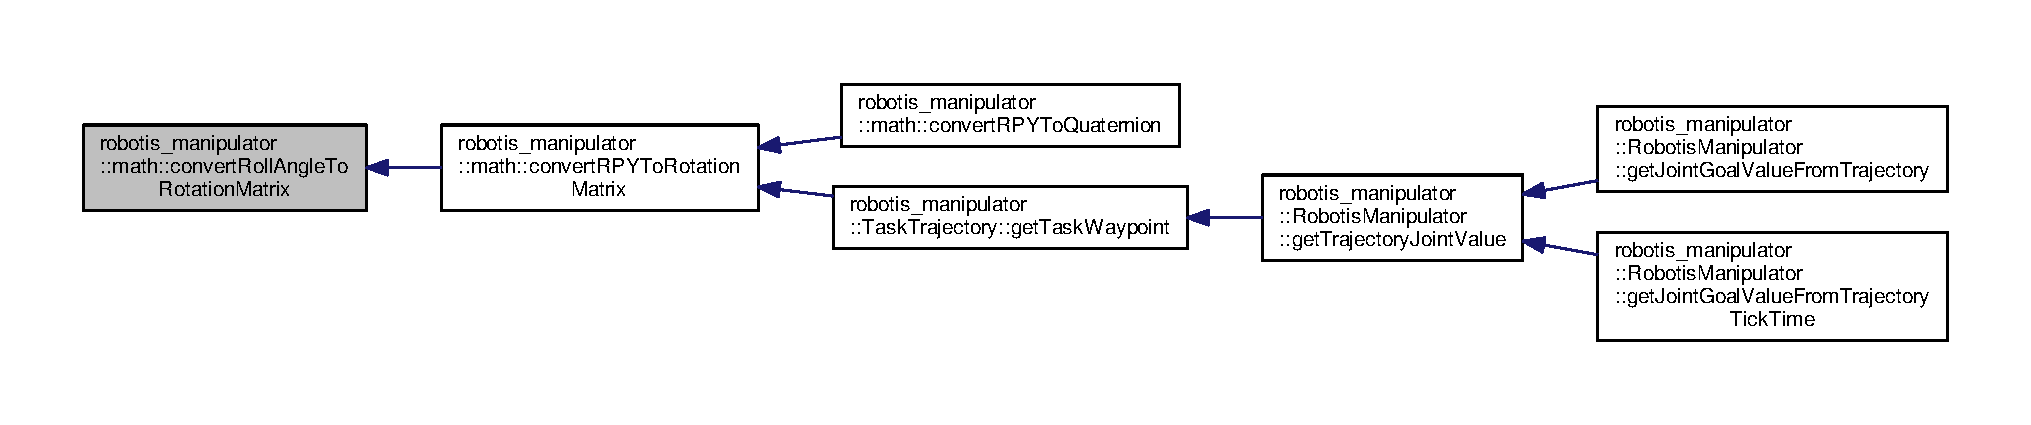
\includegraphics[width=350pt]{namespacerobotis__manipulator_1_1math_ab7682932090e254cb077badb80fe8667_icgraph}
\end{center}
\end{figure}


\index{robotis\+\_\+manipulator\+::math@{robotis\+\_\+manipulator\+::math}!convert\+Rotation\+Matrix\+To\+Omega@{convert\+Rotation\+Matrix\+To\+Omega}}
\index{convert\+Rotation\+Matrix\+To\+Omega@{convert\+Rotation\+Matrix\+To\+Omega}!robotis\+\_\+manipulator\+::math@{robotis\+\_\+manipulator\+::math}}
\subsubsection[{\texorpdfstring{convert\+Rotation\+Matrix\+To\+Omega(const Eigen\+::\+Matrix3d \&rotation\+\_\+matrix)}{convertRotationMatrixToOmega(const Eigen::Matrix3d &rotation_matrix)}}]{\setlength{\rightskip}{0pt plus 5cm}Eigen\+::\+Vector3d robotis\+\_\+manipulator\+::math\+::convert\+Rotation\+Matrix\+To\+Omega (
\begin{DoxyParamCaption}
\item[{const Eigen\+::\+Matrix3d \&}]{rotation\+\_\+matrix}
\end{DoxyParamCaption}
)}\hypertarget{namespacerobotis__manipulator_1_1math_a0659ad2d283ad43e01eca23f0be6a134}{}\label{namespacerobotis__manipulator_1_1math_a0659ad2d283ad43e01eca23f0be6a134}


convert\+Rotation\+Matrix\+To\+Omega 


\begin{DoxyParams}{Parameters}
{\em rotation\+\_\+matrix} & \\
\hline
\end{DoxyParams}
\begin{DoxyReturn}{Returns}

\end{DoxyReturn}


Definition at line 152 of file robotis\+\_\+manipulator\+\_\+math.\+cpp.


\begin{DoxyCode}
153 \{
154   \textcolor{keywordflow}{return} \hyperlink{namespacerobotis__manipulator_1_1math_a38b3c7716c5b8a29a75d8b3243eb75e7}{robotis\_manipulator::math::matrixLogarithm}(
      rotation\_matrix);
155 \}
\end{DoxyCode}


Here is the call graph for this function\+:\nopagebreak
\begin{figure}[H]
\begin{center}
\leavevmode
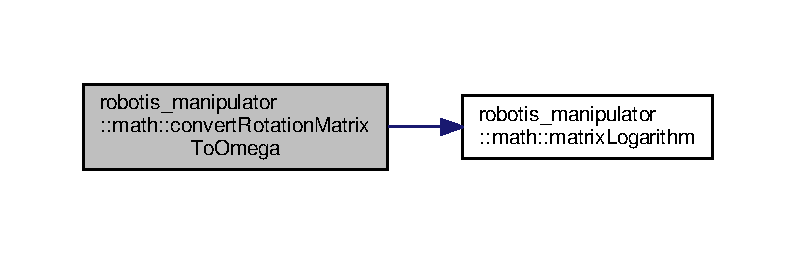
\includegraphics[width=350pt]{namespacerobotis__manipulator_1_1math_a0659ad2d283ad43e01eca23f0be6a134_cgraph}
\end{center}
\end{figure}


\index{robotis\+\_\+manipulator\+::math@{robotis\+\_\+manipulator\+::math}!convert\+Rotation\+Matrix\+To\+Quaternion@{convert\+Rotation\+Matrix\+To\+Quaternion}}
\index{convert\+Rotation\+Matrix\+To\+Quaternion@{convert\+Rotation\+Matrix\+To\+Quaternion}!robotis\+\_\+manipulator\+::math@{robotis\+\_\+manipulator\+::math}}
\subsubsection[{\texorpdfstring{convert\+Rotation\+Matrix\+To\+Quaternion(const Eigen\+::\+Matrix3d \&rotation\+\_\+matrix)}{convertRotationMatrixToQuaternion(const Eigen::Matrix3d &rotation_matrix)}}]{\setlength{\rightskip}{0pt plus 5cm}Eigen\+::\+Quaterniond robotis\+\_\+manipulator\+::math\+::convert\+Rotation\+Matrix\+To\+Quaternion (
\begin{DoxyParamCaption}
\item[{const Eigen\+::\+Matrix3d \&}]{rotation\+\_\+matrix}
\end{DoxyParamCaption}
)}\hypertarget{namespacerobotis__manipulator_1_1math_ae5a4fd98d1cef4a4b1224b19daff63bf}{}\label{namespacerobotis__manipulator_1_1math_ae5a4fd98d1cef4a4b1224b19daff63bf}


convert\+Rotation\+Matrix\+To\+Quaternion 


\begin{DoxyParams}{Parameters}
{\em rotation\+\_\+matrix} & \\
\hline
\end{DoxyParams}
\begin{DoxyReturn}{Returns}

\end{DoxyReturn}


Definition at line 130 of file robotis\+\_\+manipulator\+\_\+math.\+cpp.


\begin{DoxyCode}
131 \{
132   Eigen::Quaterniond quaternion;
133   quaternion = rotation;
134 
135   \textcolor{keywordflow}{return} quaternion;
136 \}
\end{DoxyCode}
\index{robotis\+\_\+manipulator\+::math@{robotis\+\_\+manipulator\+::math}!convert\+Rotation\+Matrix\+To\+R\+P\+Y\+Vector@{convert\+Rotation\+Matrix\+To\+R\+P\+Y\+Vector}}
\index{convert\+Rotation\+Matrix\+To\+R\+P\+Y\+Vector@{convert\+Rotation\+Matrix\+To\+R\+P\+Y\+Vector}!robotis\+\_\+manipulator\+::math@{robotis\+\_\+manipulator\+::math}}
\subsubsection[{\texorpdfstring{convert\+Rotation\+Matrix\+To\+R\+P\+Y\+Vector(const Eigen\+::\+Matrix3d \&rotation\+\_\+matrix)}{convertRotationMatrixToRPYVector(const Eigen::Matrix3d &rotation_matrix)}}]{\setlength{\rightskip}{0pt plus 5cm}Eigen\+::\+Vector3d robotis\+\_\+manipulator\+::math\+::convert\+Rotation\+Matrix\+To\+R\+P\+Y\+Vector (
\begin{DoxyParamCaption}
\item[{const Eigen\+::\+Matrix3d \&}]{rotation\+\_\+matrix}
\end{DoxyParamCaption}
)}\hypertarget{namespacerobotis__manipulator_1_1math_adaa070908c6328c2459be5eaf64af68f}{}\label{namespacerobotis__manipulator_1_1math_adaa070908c6328c2459be5eaf64af68f}


convert\+Rotation\+Matrix\+To\+R\+P\+Y\+Vector 


\begin{DoxyParams}{Parameters}
{\em rotation\+\_\+matrix} & \\
\hline
\end{DoxyParams}
\begin{DoxyReturn}{Returns}

\end{DoxyReturn}


Definition at line 105 of file robotis\+\_\+manipulator\+\_\+math.\+cpp.


\begin{DoxyCode}
106 \{
107   Eigen::Vector3d rpy;\textcolor{comment}{// = Eigen::MatrixXd::Zero(3,1);}
108   rpy.coeffRef(0,0) = atan2(rotation.coeff(2,1), rotation.coeff(2,2));
109   rpy.coeffRef(1,0) = atan2(-rotation.coeff(2,0), sqrt(pow(rotation.coeff(2,1), 2) + pow(rotation.coeff(2,2
      ),2)));
110   rpy.coeffRef(2,0) = atan2 (rotation.coeff(1,0), rotation.coeff(0,0));
111 
112   \textcolor{keywordflow}{return} rpy;
113 \}
\end{DoxyCode}


Here is the caller graph for this function\+:\nopagebreak
\begin{figure}[H]
\begin{center}
\leavevmode
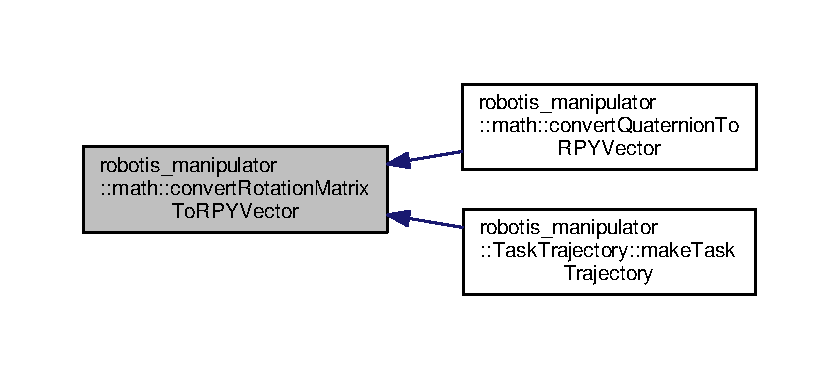
\includegraphics[width=350pt]{namespacerobotis__manipulator_1_1math_adaa070908c6328c2459be5eaf64af68f_icgraph}
\end{center}
\end{figure}


\index{robotis\+\_\+manipulator\+::math@{robotis\+\_\+manipulator\+::math}!convert\+R\+P\+Y\+Acceleration\+To\+Omega\+Dot@{convert\+R\+P\+Y\+Acceleration\+To\+Omega\+Dot}}
\index{convert\+R\+P\+Y\+Acceleration\+To\+Omega\+Dot@{convert\+R\+P\+Y\+Acceleration\+To\+Omega\+Dot}!robotis\+\_\+manipulator\+::math@{robotis\+\_\+manipulator\+::math}}
\subsubsection[{\texorpdfstring{convert\+R\+P\+Y\+Acceleration\+To\+Omega\+Dot(\+Eigen\+::\+Vector3d rpy\+\_\+vector, Eigen\+::\+Vector3d rpy\+\_\+velocity, Eigen\+::\+Vector3d rpy\+\_\+acceleration)}{convertRPYAccelerationToOmegaDot(Eigen::Vector3d rpy_vector, Eigen::Vector3d rpy_velocity, Eigen::Vector3d rpy_acceleration)}}]{\setlength{\rightskip}{0pt plus 5cm}Eigen\+::\+Vector3d robotis\+\_\+manipulator\+::math\+::convert\+R\+P\+Y\+Acceleration\+To\+Omega\+Dot (
\begin{DoxyParamCaption}
\item[{Eigen\+::\+Vector3d}]{rpy\+\_\+vector, }
\item[{Eigen\+::\+Vector3d}]{rpy\+\_\+velocity, }
\item[{Eigen\+::\+Vector3d}]{rpy\+\_\+acceleration}
\end{DoxyParamCaption}
)}\hypertarget{namespacerobotis__manipulator_1_1math_a752d1631596538515894f09f210eb17b}{}\label{namespacerobotis__manipulator_1_1math_a752d1631596538515894f09f210eb17b}


convert\+R\+P\+Y\+Acceleration\+To\+Omega\+Dot 


\begin{DoxyParams}{Parameters}
{\em rpy\+\_\+vector} & \\
\hline
{\em rpy\+\_\+velocity} & \\
\hline
{\em rpy\+\_\+acceleration} & \\
\hline
\end{DoxyParams}
\begin{DoxyReturn}{Returns}

\end{DoxyReturn}


Definition at line 284 of file robotis\+\_\+manipulator\+\_\+math.\+cpp.


\begin{DoxyCode}
285 \{
286   Eigen::Vector3d c\_dot;
287   Eigen::Matrix3d c;
288   Eigen::Vector3d omega\_dot;
289 
290   c\_dot << -cos(rpy\_vector[1]) * rpy\_velocity[1] * rpy\_velocity[2],
291            -sin(rpy\_vector[0]) * rpy\_velocity[0] * rpy\_velocity[1] - sin(rpy\_vector[0]) * sin(rpy\_vector[1]
      ) * rpy\_velocity[1] * rpy\_velocity[2] + cos(rpy\_vector[0]) * cos(rpy\_vector[1]) * rpy\_velocity[0] * 
      rpy\_velocity[2],
292            -cos(rpy\_vector[0]) * rpy\_velocity[0] * rpy\_velocity[1] - sin(rpy\_vector[0]) * cos(rpy\_vector[1]
      ) * rpy\_velocity[0] * rpy\_velocity[2] - cos(rpy\_vector[0]) * sin(rpy\_vector[1]) * rpy\_velocity[1] * 
      rpy\_velocity[2];
293 
294   c << 1, 0,                     -sin(rpy\_vector(1)),
295         0, cos(rpy\_vector(0)),    sin(rpy\_vector(0))*cos(rpy\_vector(1)),
296         0, -sin(rpy\_vector(0)), cos(rpy\_vector(0))*cos(rpy\_vector(1));
297 
298   omega\_dot = c\_dot + c * rpy\_acceleration;
299   \textcolor{keywordflow}{return} omega\_dot;
300 \}
\end{DoxyCode}


Here is the caller graph for this function\+:\nopagebreak
\begin{figure}[H]
\begin{center}
\leavevmode
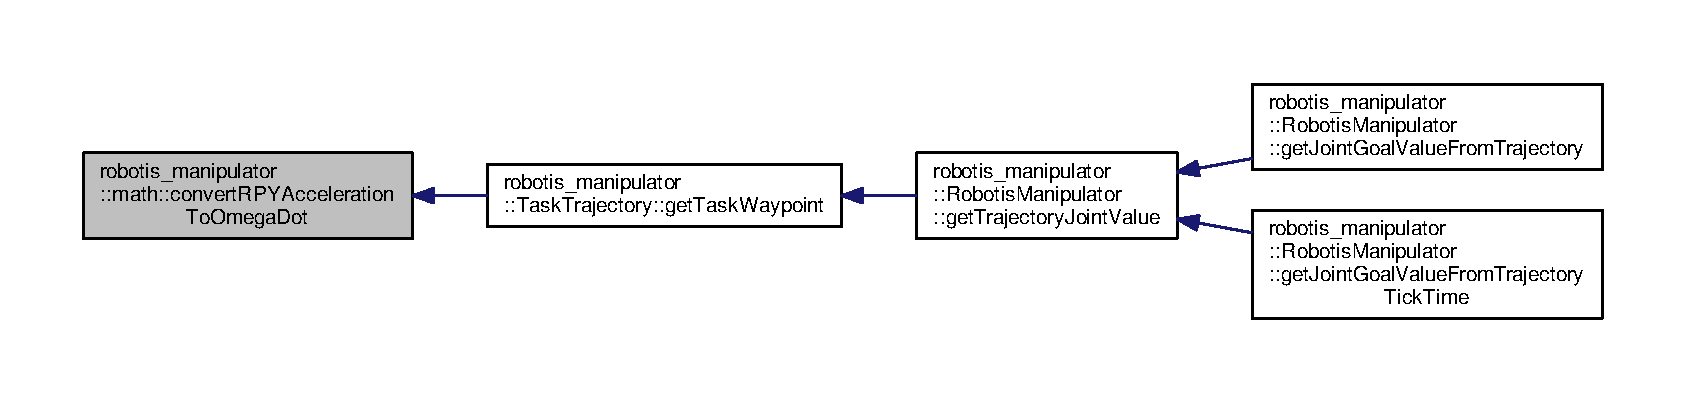
\includegraphics[width=350pt]{namespacerobotis__manipulator_1_1math_a752d1631596538515894f09f210eb17b_icgraph}
\end{center}
\end{figure}


\index{robotis\+\_\+manipulator\+::math@{robotis\+\_\+manipulator\+::math}!convert\+R\+P\+Y\+To\+Quaternion@{convert\+R\+P\+Y\+To\+Quaternion}}
\index{convert\+R\+P\+Y\+To\+Quaternion@{convert\+R\+P\+Y\+To\+Quaternion}!robotis\+\_\+manipulator\+::math@{robotis\+\_\+manipulator\+::math}}
\subsubsection[{\texorpdfstring{convert\+R\+P\+Y\+To\+Quaternion(double roll, double pitch, double yaw)}{convertRPYToQuaternion(double roll, double pitch, double yaw)}}]{\setlength{\rightskip}{0pt plus 5cm}Eigen\+::\+Quaterniond robotis\+\_\+manipulator\+::math\+::convert\+R\+P\+Y\+To\+Quaternion (
\begin{DoxyParamCaption}
\item[{double}]{roll, }
\item[{double}]{pitch, }
\item[{double}]{yaw}
\end{DoxyParamCaption}
)}\hypertarget{namespacerobotis__manipulator_1_1math_aa1d5ec03193d986594c03ab884126416}{}\label{namespacerobotis__manipulator_1_1math_aa1d5ec03193d986594c03ab884126416}


convert\+R\+P\+Y\+To\+Quaternion 


\begin{DoxyParams}{Parameters}
{\em roll} & \\
\hline
{\em pitch} & \\
\hline
{\em yaw} & \\
\hline
\end{DoxyParams}
\begin{DoxyReturn}{Returns}

\end{DoxyReturn}


Definition at line 122 of file robotis\+\_\+manipulator\+\_\+math.\+cpp.


\begin{DoxyCode}
123 \{
124  Eigen::Quaterniond quaternion;
125  quaternion = \hyperlink{namespacerobotis__manipulator_1_1math_a4bbc795e8c06dd0472ed25864f6ec886}{robotis\_manipulator::math::convertRPYToRotationMatrix}
      (roll,pitch,yaw);
126 
127  \textcolor{keywordflow}{return} quaternion;
128 \}
\end{DoxyCode}


Here is the call graph for this function\+:\nopagebreak
\begin{figure}[H]
\begin{center}
\leavevmode
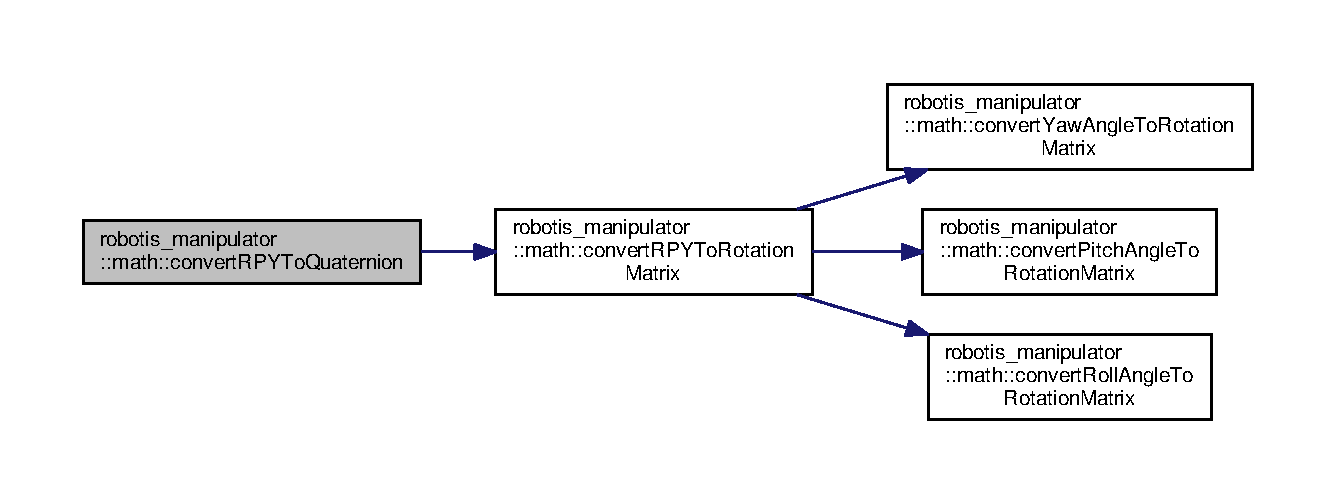
\includegraphics[width=350pt]{namespacerobotis__manipulator_1_1math_aa1d5ec03193d986594c03ab884126416_cgraph}
\end{center}
\end{figure}


\index{robotis\+\_\+manipulator\+::math@{robotis\+\_\+manipulator\+::math}!convert\+R\+P\+Y\+To\+Rotation\+Matrix@{convert\+R\+P\+Y\+To\+Rotation\+Matrix}}
\index{convert\+R\+P\+Y\+To\+Rotation\+Matrix@{convert\+R\+P\+Y\+To\+Rotation\+Matrix}!robotis\+\_\+manipulator\+::math@{robotis\+\_\+manipulator\+::math}}
\subsubsection[{\texorpdfstring{convert\+R\+P\+Y\+To\+Rotation\+Matrix(double roll, double pitch, double yaw)}{convertRPYToRotationMatrix(double roll, double pitch, double yaw)}}]{\setlength{\rightskip}{0pt plus 5cm}Eigen\+::\+Matrix3d robotis\+\_\+manipulator\+::math\+::convert\+R\+P\+Y\+To\+Rotation\+Matrix (
\begin{DoxyParamCaption}
\item[{double}]{roll, }
\item[{double}]{pitch, }
\item[{double}]{yaw}
\end{DoxyParamCaption}
)}\hypertarget{namespacerobotis__manipulator_1_1math_a4bbc795e8c06dd0472ed25864f6ec886}{}\label{namespacerobotis__manipulator_1_1math_a4bbc795e8c06dd0472ed25864f6ec886}


convert\+R\+P\+Y\+To\+Rotation\+Matrix 


\begin{DoxyParams}{Parameters}
{\em roll} & \\
\hline
{\em pitch} & \\
\hline
{\em yaw} & \\
\hline
\end{DoxyParams}
\begin{DoxyReturn}{Returns}

\end{DoxyReturn}


Definition at line 115 of file robotis\+\_\+manipulator\+\_\+math.\+cpp.


\begin{DoxyCode}
116 \{
117   Eigen::Matrix3d rotation = 
      \hyperlink{namespacerobotis__manipulator_1_1math_a0a45b10176c2a214876aa265ec8e707e}{robotis\_manipulator::math::convertYawAngleToRotationMatrix}
      (yaw)*\hyperlink{namespacerobotis__manipulator_1_1math_aa6112f12db3755d6677f45c9e0806cbf}{robotis\_manipulator::math::convertPitchAngleToRotationMatrix}
      (pitch)*\hyperlink{namespacerobotis__manipulator_1_1math_ab7682932090e254cb077badb80fe8667}{robotis\_manipulator::math::convertRollAngleToRotationMatrix}
      (roll);
118 
119   \textcolor{keywordflow}{return} rotation;
120 \}
\end{DoxyCode}


Here is the call graph for this function\+:\nopagebreak
\begin{figure}[H]
\begin{center}
\leavevmode
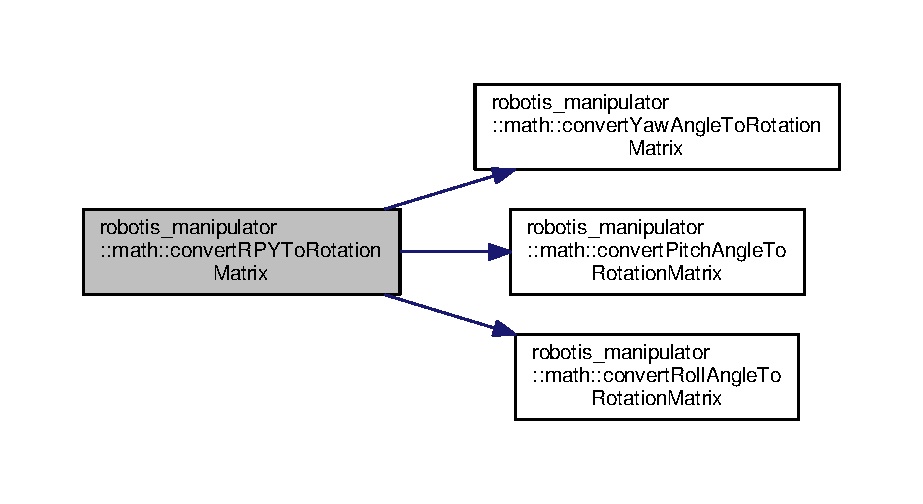
\includegraphics[width=350pt]{namespacerobotis__manipulator_1_1math_a4bbc795e8c06dd0472ed25864f6ec886_cgraph}
\end{center}
\end{figure}




Here is the caller graph for this function\+:\nopagebreak
\begin{figure}[H]
\begin{center}
\leavevmode
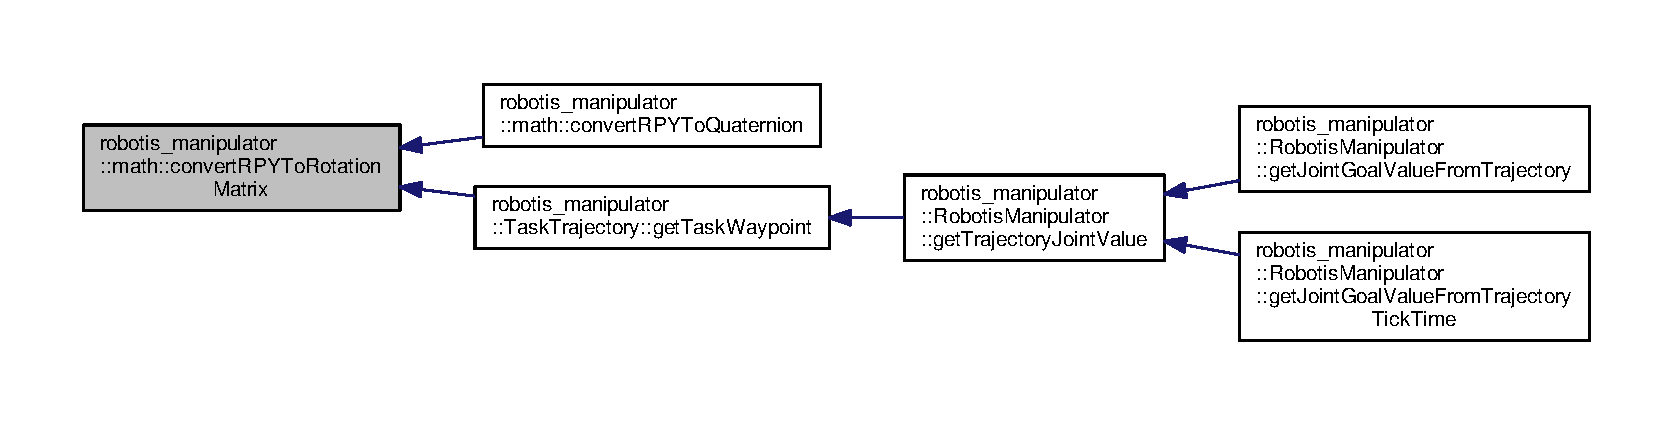
\includegraphics[width=350pt]{namespacerobotis__manipulator_1_1math_a4bbc795e8c06dd0472ed25864f6ec886_icgraph}
\end{center}
\end{figure}


\index{robotis\+\_\+manipulator\+::math@{robotis\+\_\+manipulator\+::math}!convert\+R\+P\+Y\+To\+Transformation\+Matrix@{convert\+R\+P\+Y\+To\+Transformation\+Matrix}}
\index{convert\+R\+P\+Y\+To\+Transformation\+Matrix@{convert\+R\+P\+Y\+To\+Transformation\+Matrix}!robotis\+\_\+manipulator\+::math@{robotis\+\_\+manipulator\+::math}}
\subsubsection[{\texorpdfstring{convert\+R\+P\+Y\+To\+Transformation\+Matrix(double roll, double pitch, double yaw)}{convertRPYToTransformationMatrix(double roll, double pitch, double yaw)}}]{\setlength{\rightskip}{0pt plus 5cm}Eigen\+::\+Matrix4d robotis\+\_\+manipulator\+::math\+::convert\+R\+P\+Y\+To\+Transformation\+Matrix (
\begin{DoxyParamCaption}
\item[{double}]{roll, }
\item[{double}]{pitch, }
\item[{double}]{yaw}
\end{DoxyParamCaption}
)}\hypertarget{namespacerobotis__manipulator_1_1math_a82a56f3cb0404e06bf37f2e167c839ef}{}\label{namespacerobotis__manipulator_1_1math_a82a56f3cb0404e06bf37f2e167c839ef}


convert\+R\+P\+Y\+To\+Transformation\+Matrix 


\begin{DoxyParams}{Parameters}
{\em roll} & \\
\hline
{\em pitch} & \\
\hline
{\em yaw} & \\
\hline
\end{DoxyParams}
\begin{DoxyReturn}{Returns}

\end{DoxyReturn}


Definition at line 181 of file robotis\+\_\+manipulator\+\_\+math.\+cpp.


\begin{DoxyCode}
182 \{
183   \textcolor{keywordtype}{double} sr = sin(roll), cr = cos(roll);
184   \textcolor{keywordtype}{double} sp = sin(pitch), cp = cos(pitch);
185   \textcolor{keywordtype}{double} sy = sin(yaw), cy = cos(yaw);
186 
187   Eigen::Matrix4d mat\_roll;
188   Eigen::Matrix4d mat\_pitch;
189   Eigen::Matrix4d mat\_yaw;
190 
191   mat\_roll <<
192       1, 0, 0, 0,
193       0, cr, -sr, 0,
194       0, sr, cr, 0,
195       0, 0, 0, 1;
196 
197   mat\_pitch <<
198       cp, 0, sp, 0,
199       0, 1, 0, 0,
200       -sp, 0, cp, 0,
201       0, 0, 0, 1;
202 
203   mat\_yaw <<
204       cy, -sy, 0, 0,
205       sy, cy, 0, 0,
206       0, 0, 1, 0,
207       0, 0, 0, 1;
208 
209   Eigen::Matrix4d mat\_rpy = (mat\_yaw*mat\_pitch)*mat\_roll;
210 
211   \textcolor{keywordflow}{return} mat\_rpy;
212 \}
\end{DoxyCode}


Here is the caller graph for this function\+:\nopagebreak
\begin{figure}[H]
\begin{center}
\leavevmode
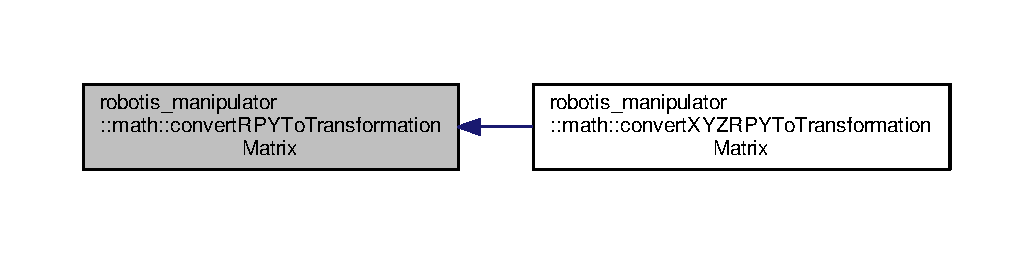
\includegraphics[width=350pt]{namespacerobotis__manipulator_1_1math_a82a56f3cb0404e06bf37f2e167c839ef_icgraph}
\end{center}
\end{figure}


\index{robotis\+\_\+manipulator\+::math@{robotis\+\_\+manipulator\+::math}!convert\+R\+P\+Y\+Velocity\+To\+Omega@{convert\+R\+P\+Y\+Velocity\+To\+Omega}}
\index{convert\+R\+P\+Y\+Velocity\+To\+Omega@{convert\+R\+P\+Y\+Velocity\+To\+Omega}!robotis\+\_\+manipulator\+::math@{robotis\+\_\+manipulator\+::math}}
\subsubsection[{\texorpdfstring{convert\+R\+P\+Y\+Velocity\+To\+Omega(\+Eigen\+::\+Vector3d rpy\+\_\+vector, Eigen\+::\+Vector3d rpy\+\_\+velocity)}{convertRPYVelocityToOmega(Eigen::Vector3d rpy_vector, Eigen::Vector3d rpy_velocity)}}]{\setlength{\rightskip}{0pt plus 5cm}Eigen\+::\+Vector3d robotis\+\_\+manipulator\+::math\+::convert\+R\+P\+Y\+Velocity\+To\+Omega (
\begin{DoxyParamCaption}
\item[{Eigen\+::\+Vector3d}]{rpy\+\_\+vector, }
\item[{Eigen\+::\+Vector3d}]{rpy\+\_\+velocity}
\end{DoxyParamCaption}
)}\hypertarget{namespacerobotis__manipulator_1_1math_a73d50f3962eeac18f464f879e6a0c8fc}{}\label{namespacerobotis__manipulator_1_1math_a73d50f3962eeac18f464f879e6a0c8fc}


convert\+R\+P\+Y\+Velocity\+To\+Omega 


\begin{DoxyParams}{Parameters}
{\em rpy\+\_\+vector} & \\
\hline
{\em rpy\+\_\+velocity} & \\
\hline
\end{DoxyParams}
\begin{DoxyReturn}{Returns}

\end{DoxyReturn}


Definition at line 253 of file robotis\+\_\+manipulator\+\_\+math.\+cpp.


\begin{DoxyCode}
254 \{
255   Eigen::Matrix3d c;
256   Eigen::Vector3d omega;
257 
258   c << 1, 0,                     -sin(rpy\_vector(1)),
259         0, cos(rpy\_vector(0)),    sin(rpy\_vector(0))*cos(rpy\_vector(1)),
260         0, -sin(rpy\_vector(0)), cos(rpy\_vector(0))*cos(rpy\_vector(1));
261 
262   omega = c * rpy\_velocity;
263   \textcolor{keywordflow}{return} omega;
264 \}
\end{DoxyCode}


Here is the caller graph for this function\+:\nopagebreak
\begin{figure}[H]
\begin{center}
\leavevmode
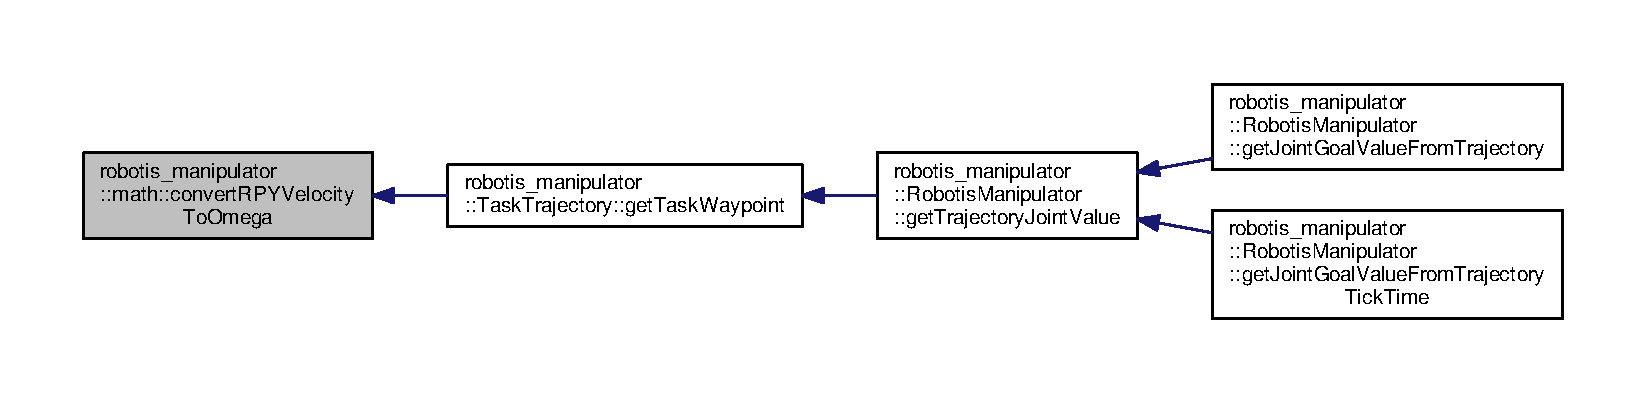
\includegraphics[width=350pt]{namespacerobotis__manipulator_1_1math_a73d50f3962eeac18f464f879e6a0c8fc_icgraph}
\end{center}
\end{figure}


\index{robotis\+\_\+manipulator\+::math@{robotis\+\_\+manipulator\+::math}!convert\+X\+Y\+Z\+R\+P\+Y\+To\+Transformation\+Matrix@{convert\+X\+Y\+Z\+R\+P\+Y\+To\+Transformation\+Matrix}}
\index{convert\+X\+Y\+Z\+R\+P\+Y\+To\+Transformation\+Matrix@{convert\+X\+Y\+Z\+R\+P\+Y\+To\+Transformation\+Matrix}!robotis\+\_\+manipulator\+::math@{robotis\+\_\+manipulator\+::math}}
\subsubsection[{\texorpdfstring{convert\+X\+Y\+Z\+R\+P\+Y\+To\+Transformation\+Matrix(double x, double y, double z, double roll, double pitch, double yaw)}{convertXYZRPYToTransformationMatrix(double x, double y, double z, double roll, double pitch, double yaw)}}]{\setlength{\rightskip}{0pt plus 5cm}Eigen\+::\+Matrix4d robotis\+\_\+manipulator\+::math\+::convert\+X\+Y\+Z\+R\+P\+Y\+To\+Transformation\+Matrix (
\begin{DoxyParamCaption}
\item[{double}]{x, }
\item[{double}]{y, }
\item[{double}]{z, }
\item[{double}]{roll, }
\item[{double}]{pitch, }
\item[{double}]{yaw}
\end{DoxyParamCaption}
)}\hypertarget{namespacerobotis__manipulator_1_1math_a5f001cf17bbf0daaaacd46f58d3f6e8a}{}\label{namespacerobotis__manipulator_1_1math_a5f001cf17bbf0daaaacd46f58d3f6e8a}


convert\+X\+Y\+Z\+R\+P\+Y\+To\+Transformation\+Matrix 


\begin{DoxyParams}{Parameters}
{\em x} & \\
\hline
{\em y} & \\
\hline
{\em z} & \\
\hline
{\em roll} & \\
\hline
{\em pitch} & \\
\hline
{\em yaw} & \\
\hline
\end{DoxyParams}
\begin{DoxyReturn}{Returns}

\end{DoxyReturn}


Definition at line 158 of file robotis\+\_\+manipulator\+\_\+math.\+cpp.


\begin{DoxyCode}
159 \{
160   Eigen::Matrix4d transformation = 
      \hyperlink{namespacerobotis__manipulator_1_1math_a82a56f3cb0404e06bf37f2e167c839ef}{robotis\_manipulator::math::convertRPYToTransformationMatrix}
      (roll, pitch, yaw);
161   transformation.coeffRef(0,3) = position\_x;
162   transformation.coeffRef(1,3) = position\_y;
163   transformation.coeffRef(2,3) = position\_z;
164 
165   \textcolor{keywordflow}{return} transformation;
166 \}
\end{DoxyCode}


Here is the call graph for this function\+:\nopagebreak
\begin{figure}[H]
\begin{center}
\leavevmode
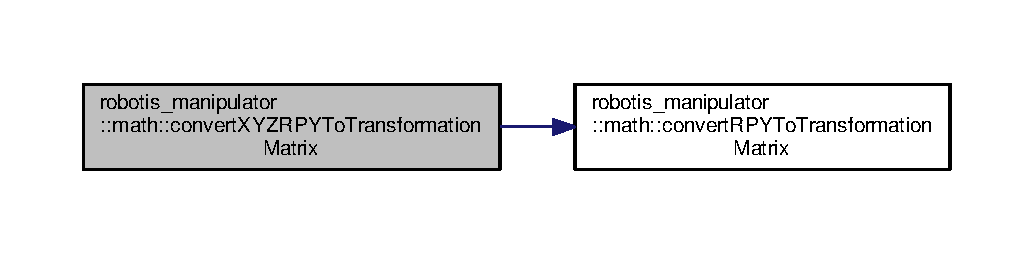
\includegraphics[width=350pt]{namespacerobotis__manipulator_1_1math_a5f001cf17bbf0daaaacd46f58d3f6e8a_cgraph}
\end{center}
\end{figure}


\index{robotis\+\_\+manipulator\+::math@{robotis\+\_\+manipulator\+::math}!convert\+X\+Y\+Z\+To\+Transformation\+Matrix@{convert\+X\+Y\+Z\+To\+Transformation\+Matrix}}
\index{convert\+X\+Y\+Z\+To\+Transformation\+Matrix@{convert\+X\+Y\+Z\+To\+Transformation\+Matrix}!robotis\+\_\+manipulator\+::math@{robotis\+\_\+manipulator\+::math}}
\subsubsection[{\texorpdfstring{convert\+X\+Y\+Z\+To\+Transformation\+Matrix(double x, double y, double z)}{convertXYZToTransformationMatrix(double x, double y, double z)}}]{\setlength{\rightskip}{0pt plus 5cm}Eigen\+::\+Matrix4d robotis\+\_\+manipulator\+::math\+::convert\+X\+Y\+Z\+To\+Transformation\+Matrix (
\begin{DoxyParamCaption}
\item[{double}]{x, }
\item[{double}]{y, }
\item[{double}]{z}
\end{DoxyParamCaption}
)}\hypertarget{namespacerobotis__manipulator_1_1math_a0e864bea906520574b93496db74427f0}{}\label{namespacerobotis__manipulator_1_1math_a0e864bea906520574b93496db74427f0}


convert\+X\+Y\+Z\+To\+Transformation\+Matrix 


\begin{DoxyParams}{Parameters}
{\em x} & \\
\hline
{\em y} & \\
\hline
{\em z} & \\
\hline
\end{DoxyParams}
\begin{DoxyReturn}{Returns}

\end{DoxyReturn}


Definition at line 168 of file robotis\+\_\+manipulator\+\_\+math.\+cpp.


\begin{DoxyCode}
169 \{
170   Eigen::Matrix4d mat\_translation;
171 
172   mat\_translation <<
173       1, 0, 0, position\_x,
174       0, 1, 0, position\_y,
175       0, 0, 1, position\_z,
176       0, 0, 0,          1;
177 
178   \textcolor{keywordflow}{return} mat\_translation;
179 \}
\end{DoxyCode}
\index{robotis\+\_\+manipulator\+::math@{robotis\+\_\+manipulator\+::math}!convert\+X\+Y\+Z\+To\+Vector@{convert\+X\+Y\+Z\+To\+Vector}}
\index{convert\+X\+Y\+Z\+To\+Vector@{convert\+X\+Y\+Z\+To\+Vector}!robotis\+\_\+manipulator\+::math@{robotis\+\_\+manipulator\+::math}}
\subsubsection[{\texorpdfstring{convert\+X\+Y\+Z\+To\+Vector(double x, double y, double z)}{convertXYZToVector(double x, double y, double z)}}]{\setlength{\rightskip}{0pt plus 5cm}Eigen\+::\+Vector3d robotis\+\_\+manipulator\+::math\+::convert\+X\+Y\+Z\+To\+Vector (
\begin{DoxyParamCaption}
\item[{double}]{x, }
\item[{double}]{y, }
\item[{double}]{z}
\end{DoxyParamCaption}
)}\hypertarget{namespacerobotis__manipulator_1_1math_acb3c85751c21502d8d23a13cc08b3cf5}{}\label{namespacerobotis__manipulator_1_1math_acb3c85751c21502d8d23a13cc08b3cf5}


convert\+X\+Y\+Z\+To\+Vector 


\begin{DoxyParams}{Parameters}
{\em x} & \\
\hline
{\em y} & \\
\hline
{\em z} & \\
\hline
\end{DoxyParams}
\begin{DoxyReturn}{Returns}

\end{DoxyReturn}


Definition at line 63 of file robotis\+\_\+manipulator\+\_\+math.\+cpp.


\begin{DoxyCode}
64 \{
65   Eigen::Vector3d position;
66   position << x, y, z;
67 
68   \textcolor{keywordflow}{return} position;
69 \}
\end{DoxyCode}
\index{robotis\+\_\+manipulator\+::math@{robotis\+\_\+manipulator\+::math}!convert\+Yaw\+Angle\+To\+Rotation\+Matrix@{convert\+Yaw\+Angle\+To\+Rotation\+Matrix}}
\index{convert\+Yaw\+Angle\+To\+Rotation\+Matrix@{convert\+Yaw\+Angle\+To\+Rotation\+Matrix}!robotis\+\_\+manipulator\+::math@{robotis\+\_\+manipulator\+::math}}
\subsubsection[{\texorpdfstring{convert\+Yaw\+Angle\+To\+Rotation\+Matrix(double angle)}{convertYawAngleToRotationMatrix(double angle)}}]{\setlength{\rightskip}{0pt plus 5cm}Eigen\+::\+Matrix3d robotis\+\_\+manipulator\+::math\+::convert\+Yaw\+Angle\+To\+Rotation\+Matrix (
\begin{DoxyParamCaption}
\item[{double}]{angle}
\end{DoxyParamCaption}
)}\hypertarget{namespacerobotis__manipulator_1_1math_a0a45b10176c2a214876aa265ec8e707e}{}\label{namespacerobotis__manipulator_1_1math_a0a45b10176c2a214876aa265ec8e707e}


convert\+Yaw\+Angle\+To\+Rotation\+Matrix 


\begin{DoxyParams}{Parameters}
{\em angle} & \\
\hline
\end{DoxyParams}
\begin{DoxyReturn}{Returns}

\end{DoxyReturn}


Definition at line 94 of file robotis\+\_\+manipulator\+\_\+math.\+cpp.


\begin{DoxyCode}
95 \{
96   Eigen::Matrix3d rotation(3,3);
97   rotation <<
98       cos(angle), -sin(angle), 0.0,
99       sin(angle), cos(angle), 0.0,
100       0.0, 0.0, 1.0;
101 
102   \textcolor{keywordflow}{return} rotation;
103 \}
\end{DoxyCode}


Here is the caller graph for this function\+:\nopagebreak
\begin{figure}[H]
\begin{center}
\leavevmode
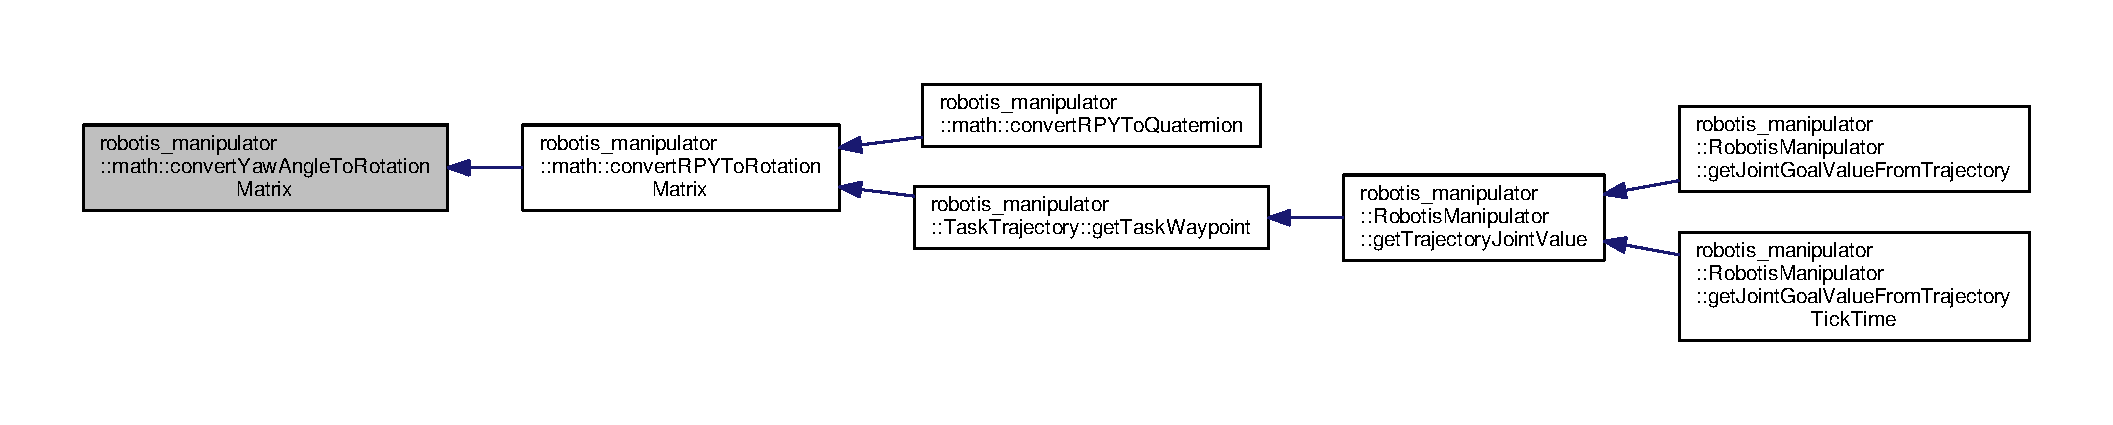
\includegraphics[width=350pt]{namespacerobotis__manipulator_1_1math_a0a45b10176c2a214876aa265ec8e707e_icgraph}
\end{center}
\end{figure}


\index{robotis\+\_\+manipulator\+::math@{robotis\+\_\+manipulator\+::math}!inertia\+Matrix@{inertia\+Matrix}}
\index{inertia\+Matrix@{inertia\+Matrix}!robotis\+\_\+manipulator\+::math@{robotis\+\_\+manipulator\+::math}}
\subsubsection[{\texorpdfstring{inertia\+Matrix(double ixx, double ixy, double ixz, double iyy, double iyz, double izz)}{inertiaMatrix(double ixx, double ixy, double ixz, double iyy, double iyz, double izz)}}]{\setlength{\rightskip}{0pt plus 5cm}Eigen\+::\+Matrix3d robotis\+\_\+manipulator\+::math\+::inertia\+Matrix (
\begin{DoxyParamCaption}
\item[{double}]{ixx, }
\item[{double}]{ixy, }
\item[{double}]{ixz, }
\item[{double}]{iyy, }
\item[{double}]{iyz, }
\item[{double}]{izz}
\end{DoxyParamCaption}
)}\hypertarget{namespacerobotis__manipulator_1_1math_a34ebf1c9f0f64e52807fd9798a7d87c8}{}\label{namespacerobotis__manipulator_1_1math_a34ebf1c9f0f64e52807fd9798a7d87c8}


inertia\+Matrix 


\begin{DoxyParams}{Parameters}
{\em ixx} & \\
\hline
{\em ixy} & \\
\hline
{\em ixz} & \\
\hline
{\em iyy} & \\
\hline
{\em iyz} & \\
\hline
{\em izz} & \\
\hline
\end{DoxyParams}
\begin{DoxyReturn}{Returns}

\end{DoxyReturn}


Definition at line 47 of file robotis\+\_\+manipulator\+\_\+math.\+cpp.


\begin{DoxyCode}
48 \{
49   Eigen::Matrix3d inertia;
50   inertia <<
51       ixx, ixy, ixz,
52       ixy, iyy, iyz,
53       ixz, iyz, izz;
54 
55   \textcolor{keywordflow}{return} inertia;
56 \}
\end{DoxyCode}
\index{robotis\+\_\+manipulator\+::math@{robotis\+\_\+manipulator\+::math}!inverse\+Transformation\+Matrix@{inverse\+Transformation\+Matrix}}
\index{inverse\+Transformation\+Matrix@{inverse\+Transformation\+Matrix}!robotis\+\_\+manipulator\+::math@{robotis\+\_\+manipulator\+::math}}
\subsubsection[{\texorpdfstring{inverse\+Transformation\+Matrix(const Eigen\+::\+Matrix\+Xd \&transformation\+\_\+matrix)}{inverseTransformationMatrix(const Eigen::MatrixXd &transformation_matrix)}}]{\setlength{\rightskip}{0pt plus 5cm}Eigen\+::\+Matrix4d robotis\+\_\+manipulator\+::math\+::inverse\+Transformation\+Matrix (
\begin{DoxyParamCaption}
\item[{const Eigen\+::\+Matrix\+Xd \&}]{transformation\+\_\+matrix}
\end{DoxyParamCaption}
)}\hypertarget{namespacerobotis__manipulator_1_1math_a0e23b77220a7f83814de154838a47be7}{}\label{namespacerobotis__manipulator_1_1math_a0e23b77220a7f83814de154838a47be7}


inverse\+Transformation\+Matrix 


\begin{DoxyParams}{Parameters}
{\em transformation\+\_\+matrix} & \\
\hline
\end{DoxyParams}
\begin{DoxyReturn}{Returns}

\end{DoxyReturn}


Definition at line 214 of file robotis\+\_\+manipulator\+\_\+math.\+cpp.


\begin{DoxyCode}
215 \{
216   \textcolor{comment}{// If T is Transform Matrix A from B, the BOA is translation component coordi. B to coordi. A}
217 
218   Eigen::Vector3d vec\_boa;
219   Eigen::Vector3d vec\_x, vec\_y, vec\_z;
220   Eigen::Matrix4d inv\_t;
221 
222   vec\_boa(0) = -transform(0,3);
223   vec\_boa(1) = -transform(1,3);
224   vec\_boa(2) = -transform(2,3);
225 
226   vec\_x(0) = transform(0,0); vec\_x(1) = transform(1,0); vec\_x(2) = transform(2,0);
227   vec\_y(0) = transform(0,1); vec\_y(1) = transform(1,1); vec\_y(2) = transform(2,1);
228   vec\_z(0) = transform(0,2); vec\_z(1) = transform(1,2); vec\_z(2) = transform(2,2);
229 
230   inv\_t <<
231       vec\_x(0), vec\_x(1), vec\_x(2), vec\_boa.dot(vec\_x),
232       vec\_y(0), vec\_y(1), vec\_y(2), vec\_boa.dot(vec\_y),
233       vec\_z(0), vec\_z(1), vec\_z(2), vec\_boa.dot(vec\_z),
234       0, 0, 0, 1;
235 
236   \textcolor{keywordflow}{return} inv\_t;
237 \}
\end{DoxyCode}
\index{robotis\+\_\+manipulator\+::math@{robotis\+\_\+manipulator\+::math}!matrix3@{matrix3}}
\index{matrix3@{matrix3}!robotis\+\_\+manipulator\+::math@{robotis\+\_\+manipulator\+::math}}
\subsubsection[{\texorpdfstring{matrix3(double m11, double m12, double m13, double m21, double m22, double m23, double m31, double m32, double m33)}{matrix3(double m11, double m12, double m13, double m21, double m22, double m23, double m31, double m32, double m33)}}]{\setlength{\rightskip}{0pt plus 5cm}Eigen\+::\+Matrix3d robotis\+\_\+manipulator\+::math\+::matrix3 (
\begin{DoxyParamCaption}
\item[{double}]{m11, }
\item[{double}]{m12, }
\item[{double}]{m13, }
\item[{double}]{m21, }
\item[{double}]{m22, }
\item[{double}]{m23, }
\item[{double}]{m31, }
\item[{double}]{m32, }
\item[{double}]{m33}
\end{DoxyParamCaption}
)}\hypertarget{namespacerobotis__manipulator_1_1math_a22fb2daaef2f7943fa0dbd7a24e0fd4d}{}\label{namespacerobotis__manipulator_1_1math_a22fb2daaef2f7943fa0dbd7a24e0fd4d}


matrix3 


\begin{DoxyParams}{Parameters}
{\em m11} & \\
\hline
{\em m12} & \\
\hline
{\em m13} & \\
\hline
{\em m21} & \\
\hline
{\em m22} & \\
\hline
{\em m23} & \\
\hline
{\em m31} & \\
\hline
{\em m32} & \\
\hline
{\em m33} & \\
\hline
\end{DoxyParams}
\begin{DoxyReturn}{Returns}

\end{DoxyReturn}


Definition at line 38 of file robotis\+\_\+manipulator\+\_\+math.\+cpp.


\begin{DoxyCode}
41 \{
42   Eigen::Matrix3d temp;
43   temp << m11, m12, m13, m21, m22, m23, m31, m32, m33;
44   \textcolor{keywordflow}{return} temp;
45 \}
\end{DoxyCode}
\index{robotis\+\_\+manipulator\+::math@{robotis\+\_\+manipulator\+::math}!matrix\+Logarithm@{matrix\+Logarithm}}
\index{matrix\+Logarithm@{matrix\+Logarithm}!robotis\+\_\+manipulator\+::math@{robotis\+\_\+manipulator\+::math}}
\subsubsection[{\texorpdfstring{matrix\+Logarithm(\+Eigen\+::\+Matrix3d rotation\+\_\+matrix)}{matrixLogarithm(Eigen::Matrix3d rotation_matrix)}}]{\setlength{\rightskip}{0pt plus 5cm}Eigen\+::\+Vector3d robotis\+\_\+manipulator\+::math\+::matrix\+Logarithm (
\begin{DoxyParamCaption}
\item[{Eigen\+::\+Matrix3d}]{rotation\+\_\+matrix}
\end{DoxyParamCaption}
)}\hypertarget{namespacerobotis__manipulator_1_1math_a38b3c7716c5b8a29a75d8b3243eb75e7}{}\label{namespacerobotis__manipulator_1_1math_a38b3c7716c5b8a29a75d8b3243eb75e7}


matrix\+Logarithm 


\begin{DoxyParams}{Parameters}
{\em rotation\+\_\+matrix} & \\
\hline
\end{DoxyParams}
\begin{DoxyReturn}{Returns}

\end{DoxyReturn}


Definition at line 318 of file robotis\+\_\+manipulator\+\_\+math.\+cpp.


\begin{DoxyCode}
319 \{
320   Eigen::Matrix3d R = rotation\_matrix;
321   Eigen::Vector3d l = Eigen::Vector3d::Zero();
322   Eigen::Vector3d rotation\_vector = Eigen::Vector3d::Zero();
323 
324   \textcolor{keywordtype}{double} theta = 0.0;
325   \textcolor{comment}{// double diag = 0.0;}
326   \textcolor{keywordtype}{bool} diagonal\_matrix = R.isDiagonal();
327 
328   l << R(2, 1) - R(1, 2),
329       R(0, 2) - R(2, 0),
330       R(1, 0) - R(0, 1);
331   theta = atan2(l.norm(), R(0, 0) + R(1, 1) + R(2, 2) - 1);
332   \textcolor{comment}{// diag = R.determinant();}
333 
334   \textcolor{keywordflow}{if} (R.isIdentity())
335   \{
336     rotation\_vector.setZero(3);
337     \textcolor{keywordflow}{return} rotation\_vector;
338   \}
339   
340   \textcolor{keywordflow}{if} (diagonal\_matrix == \textcolor{keyword}{true})
341   \{
342     rotation\_vector << R(0, 0) + 1, R(1, 1) + 1, R(2, 2) + 1;
343     rotation\_vector = rotation\_vector * M\_PI\_2;
344   \}
345   \textcolor{keywordflow}{else}
346   \{
347     rotation\_vector = theta * (l / l.norm());
348   \}
349   \textcolor{keywordflow}{return} rotation\_vector;
350 \}
\end{DoxyCode}


Here is the caller graph for this function\+:\nopagebreak
\begin{figure}[H]
\begin{center}
\leavevmode
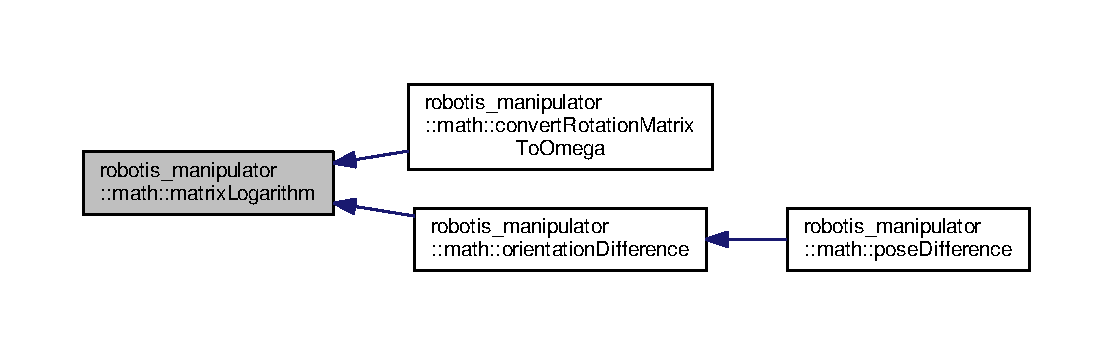
\includegraphics[width=350pt]{namespacerobotis__manipulator_1_1math_a38b3c7716c5b8a29a75d8b3243eb75e7_icgraph}
\end{center}
\end{figure}


\index{robotis\+\_\+manipulator\+::math@{robotis\+\_\+manipulator\+::math}!orientation\+Difference@{orientation\+Difference}}
\index{orientation\+Difference@{orientation\+Difference}!robotis\+\_\+manipulator\+::math@{robotis\+\_\+manipulator\+::math}}
\subsubsection[{\texorpdfstring{orientation\+Difference(\+Eigen\+::\+Matrix3d desired\+\_\+orientation, Eigen\+::\+Matrix3d present\+\_\+orientation)}{orientationDifference(Eigen::Matrix3d desired_orientation, Eigen::Matrix3d present_orientation)}}]{\setlength{\rightskip}{0pt plus 5cm}Eigen\+::\+Vector3d robotis\+\_\+manipulator\+::math\+::orientation\+Difference (
\begin{DoxyParamCaption}
\item[{Eigen\+::\+Matrix3d}]{desired\+\_\+orientation, }
\item[{Eigen\+::\+Matrix3d}]{present\+\_\+orientation}
\end{DoxyParamCaption}
)}\hypertarget{namespacerobotis__manipulator_1_1math_a26796dad948a40bc2c0ac2c139ed85f0}{}\label{namespacerobotis__manipulator_1_1math_a26796dad948a40bc2c0ac2c139ed85f0}


orientation\+Difference 


\begin{DoxyParams}{Parameters}
{\em desired\+\_\+orientation} & \\
\hline
{\em present\+\_\+orientation} & \\
\hline
\end{DoxyParams}
\begin{DoxyReturn}{Returns}

\end{DoxyReturn}


Definition at line 382 of file robotis\+\_\+manipulator\+\_\+math.\+cpp.


\begin{DoxyCode}
383 \{
384   Eigen::Vector3d orientation\_difference;
385   orientation\_difference = present\_orientation * 
      \hyperlink{namespacerobotis__manipulator_1_1math_a38b3c7716c5b8a29a75d8b3243eb75e7}{robotis\_manipulator::math::matrixLogarithm}(present\_orientation.
      transpose() * desired\_orientation);
386 
387   \textcolor{keywordflow}{return} orientation\_difference;
388 \}
\end{DoxyCode}


Here is the call graph for this function\+:\nopagebreak
\begin{figure}[H]
\begin{center}
\leavevmode
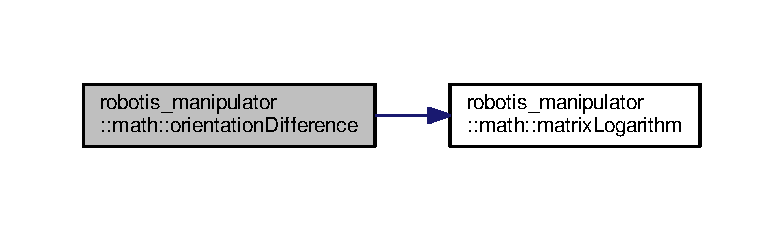
\includegraphics[width=350pt]{namespacerobotis__manipulator_1_1math_a26796dad948a40bc2c0ac2c139ed85f0_cgraph}
\end{center}
\end{figure}




Here is the caller graph for this function\+:\nopagebreak
\begin{figure}[H]
\begin{center}
\leavevmode
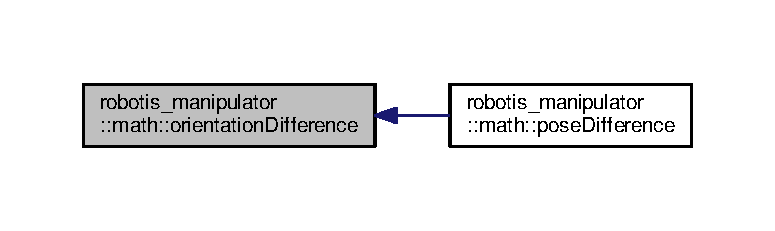
\includegraphics[width=350pt]{namespacerobotis__manipulator_1_1math_a26796dad948a40bc2c0ac2c139ed85f0_icgraph}
\end{center}
\end{figure}


\index{robotis\+\_\+manipulator\+::math@{robotis\+\_\+manipulator\+::math}!pose\+Difference@{pose\+Difference}}
\index{pose\+Difference@{pose\+Difference}!robotis\+\_\+manipulator\+::math@{robotis\+\_\+manipulator\+::math}}
\subsubsection[{\texorpdfstring{pose\+Difference(\+Eigen\+::\+Vector3d desired\+\_\+position, Eigen\+::\+Vector3d present\+\_\+position, Eigen\+::\+Matrix3d desired\+\_\+orientation, Eigen\+::\+Matrix3d present\+\_\+orientation)}{poseDifference(Eigen::Vector3d desired_position, Eigen::Vector3d present_position, Eigen::Matrix3d desired_orientation, Eigen::Matrix3d present_orientation)}}]{\setlength{\rightskip}{0pt plus 5cm}Eigen\+::\+Vector\+Xd robotis\+\_\+manipulator\+::math\+::pose\+Difference (
\begin{DoxyParamCaption}
\item[{Eigen\+::\+Vector3d}]{desired\+\_\+position, }
\item[{Eigen\+::\+Vector3d}]{present\+\_\+position, }
\item[{Eigen\+::\+Matrix3d}]{desired\+\_\+orientation, }
\item[{Eigen\+::\+Matrix3d}]{present\+\_\+orientation}
\end{DoxyParamCaption}
)}\hypertarget{namespacerobotis__manipulator_1_1math_a5bf9202c405abf15e234505842bf7361}{}\label{namespacerobotis__manipulator_1_1math_a5bf9202c405abf15e234505842bf7361}


pose\+Difference 


\begin{DoxyParams}{Parameters}
{\em desired\+\_\+position} & \\
\hline
{\em present\+\_\+position} & \\
\hline
{\em desired\+\_\+orientation} & \\
\hline
{\em present\+\_\+orientation} & \\
\hline
\end{DoxyParams}
\begin{DoxyReturn}{Returns}

\end{DoxyReturn}


Definition at line 390 of file robotis\+\_\+manipulator\+\_\+math.\+cpp.


\begin{DoxyCode}
392 \{
393   Eigen::Vector3d position\_difference;
394   Eigen::Vector3d orientation\_difference;
395   Eigen::VectorXd pose\_difference(6);
396 
397   position\_difference = \hyperlink{namespacerobotis__manipulator_1_1math_ab4f15d22dddddc5f712de188ba0f85f4}{robotis\_manipulator::math::positionDifference}
      (desired\_position, present\_position);
398   orientation\_difference = \hyperlink{namespacerobotis__manipulator_1_1math_a26796dad948a40bc2c0ac2c139ed85f0}{robotis\_manipulator::math::orientationDifference}
      (desired\_orientation, present\_orientation);
399   pose\_difference << position\_difference(0), position\_difference(1), position\_difference(2),
400       orientation\_difference(0), orientation\_difference(1), orientation\_difference(2);
401 
402   \textcolor{keywordflow}{return} pose\_difference;
403 \}
\end{DoxyCode}


Here is the call graph for this function\+:\nopagebreak
\begin{figure}[H]
\begin{center}
\leavevmode
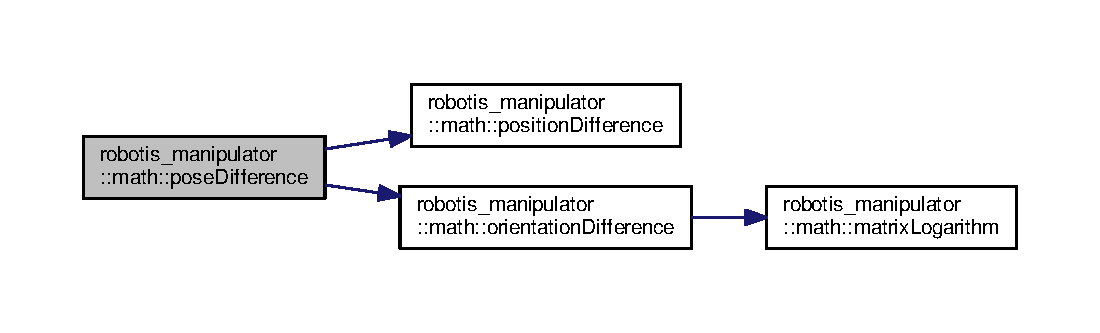
\includegraphics[width=350pt]{namespacerobotis__manipulator_1_1math_a5bf9202c405abf15e234505842bf7361_cgraph}
\end{center}
\end{figure}


\index{robotis\+\_\+manipulator\+::math@{robotis\+\_\+manipulator\+::math}!position\+Difference@{position\+Difference}}
\index{position\+Difference@{position\+Difference}!robotis\+\_\+manipulator\+::math@{robotis\+\_\+manipulator\+::math}}
\subsubsection[{\texorpdfstring{position\+Difference(\+Eigen\+::\+Vector3d desired\+\_\+position, Eigen\+::\+Vector3d present\+\_\+position)}{positionDifference(Eigen::Vector3d desired_position, Eigen::Vector3d present_position)}}]{\setlength{\rightskip}{0pt plus 5cm}Eigen\+::\+Vector3d robotis\+\_\+manipulator\+::math\+::position\+Difference (
\begin{DoxyParamCaption}
\item[{Eigen\+::\+Vector3d}]{desired\+\_\+position, }
\item[{Eigen\+::\+Vector3d}]{present\+\_\+position}
\end{DoxyParamCaption}
)}\hypertarget{namespacerobotis__manipulator_1_1math_ab4f15d22dddddc5f712de188ba0f85f4}{}\label{namespacerobotis__manipulator_1_1math_ab4f15d22dddddc5f712de188ba0f85f4}


position\+Difference 


\begin{DoxyParams}{Parameters}
{\em desired\+\_\+position} & \\
\hline
{\em present\+\_\+position} & \\
\hline
\end{DoxyParams}
\begin{DoxyReturn}{Returns}

\end{DoxyReturn}


Definition at line 374 of file robotis\+\_\+manipulator\+\_\+math.\+cpp.


\begin{DoxyCode}
375 \{
376   Eigen::Vector3d position\_difference;
377   position\_difference = desired\_position - present\_position;
378 
379   \textcolor{keywordflow}{return} position\_difference;
380 \}
\end{DoxyCode}


Here is the caller graph for this function\+:\nopagebreak
\begin{figure}[H]
\begin{center}
\leavevmode
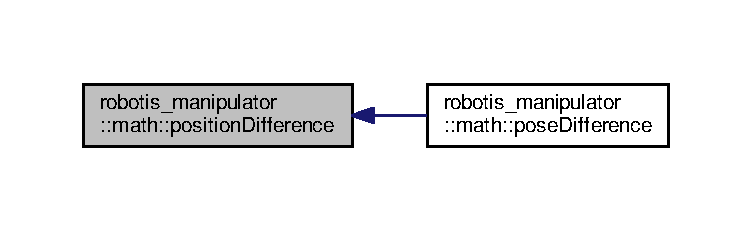
\includegraphics[width=350pt]{namespacerobotis__manipulator_1_1math_ab4f15d22dddddc5f712de188ba0f85f4_icgraph}
\end{center}
\end{figure}


\index{robotis\+\_\+manipulator\+::math@{robotis\+\_\+manipulator\+::math}!rodrigues\+Rotation\+Matrix@{rodrigues\+Rotation\+Matrix}}
\index{rodrigues\+Rotation\+Matrix@{rodrigues\+Rotation\+Matrix}!robotis\+\_\+manipulator\+::math@{robotis\+\_\+manipulator\+::math}}
\subsubsection[{\texorpdfstring{rodrigues\+Rotation\+Matrix(\+Eigen\+::\+Vector3d axis, double angle)}{rodriguesRotationMatrix(Eigen::Vector3d axis, double angle)}}]{\setlength{\rightskip}{0pt plus 5cm}Eigen\+::\+Matrix3d robotis\+\_\+manipulator\+::math\+::rodrigues\+Rotation\+Matrix (
\begin{DoxyParamCaption}
\item[{Eigen\+::\+Vector3d}]{axis, }
\item[{double}]{angle}
\end{DoxyParamCaption}
)}\hypertarget{namespacerobotis__manipulator_1_1math_a515d31a7d3b19cce814cd121717bcb60}{}\label{namespacerobotis__manipulator_1_1math_a515d31a7d3b19cce814cd121717bcb60}


rodrigues\+Rotation\+Matrix 


\begin{DoxyParams}{Parameters}
{\em axis} & \\
\hline
{\em angle} & \\
\hline
\end{DoxyParams}
\begin{DoxyReturn}{Returns}

\end{DoxyReturn}


Definition at line 361 of file robotis\+\_\+manipulator\+\_\+math.\+cpp.


\begin{DoxyCode}
362 \{
363   Eigen::Matrix3d skew\_symmetric\_matrix = Eigen::Matrix3d::Zero();
364   Eigen::Matrix3d rotation\_matrix = Eigen::Matrix3d::Zero();
365   Eigen::Matrix3d Identity\_matrix = Eigen::Matrix3d::Identity();
366 
367   skew\_symmetric\_matrix = \hyperlink{namespacerobotis__manipulator_1_1math_a03bf0fffc828339f2216fd4a98a32923}{robotis\_manipulator::math::skewSymmetricMatrix}
      (axis);
368   rotation\_matrix = Identity\_matrix +
369                     skew\_symmetric\_matrix * sin(angle) +
370                     skew\_symmetric\_matrix * skew\_symmetric\_matrix * (1 - cos(angle));
371   \textcolor{keywordflow}{return} rotation\_matrix;
372 \}
\end{DoxyCode}


Here is the call graph for this function\+:\nopagebreak
\begin{figure}[H]
\begin{center}
\leavevmode
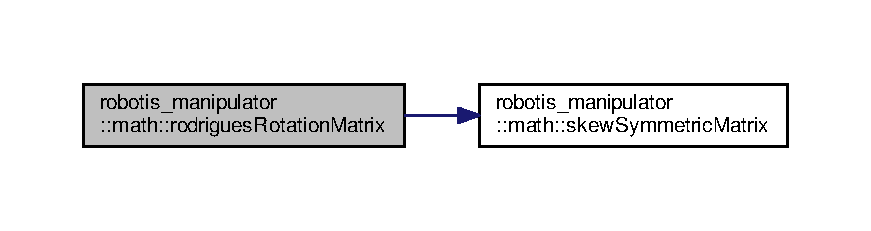
\includegraphics[width=350pt]{namespacerobotis__manipulator_1_1math_a515d31a7d3b19cce814cd121717bcb60_cgraph}
\end{center}
\end{figure}


\index{robotis\+\_\+manipulator\+::math@{robotis\+\_\+manipulator\+::math}!sign@{sign}}
\index{sign@{sign}!robotis\+\_\+manipulator\+::math@{robotis\+\_\+manipulator\+::math}}
\subsubsection[{\texorpdfstring{sign(double value)}{sign(double value)}}]{\setlength{\rightskip}{0pt plus 5cm}double robotis\+\_\+manipulator\+::math\+::sign (
\begin{DoxyParamCaption}
\item[{double}]{value}
\end{DoxyParamCaption}
)}\hypertarget{namespacerobotis__manipulator_1_1math_a27a6dd481239e8377185dac85cf9cd77}{}\label{namespacerobotis__manipulator_1_1math_a27a6dd481239e8377185dac85cf9cd77}


sign 


\begin{DoxyParams}{Parameters}
{\em value} & \\
\hline
\end{DoxyParams}
\begin{DoxyReturn}{Returns}

\end{DoxyReturn}


Definition at line 306 of file robotis\+\_\+manipulator\+\_\+math.\+cpp.


\begin{DoxyCode}
307 \{
308   \textcolor{keywordflow}{if} (value >= 0.0)
309   \{
310     \textcolor{keywordflow}{return} 1.0;
311   \}
312   \textcolor{keywordflow}{else}
313   \{
314     \textcolor{keywordflow}{return} -1.0;
315   \}
316 \}
\end{DoxyCode}
\index{robotis\+\_\+manipulator\+::math@{robotis\+\_\+manipulator\+::math}!skew\+Symmetric\+Matrix@{skew\+Symmetric\+Matrix}}
\index{skew\+Symmetric\+Matrix@{skew\+Symmetric\+Matrix}!robotis\+\_\+manipulator\+::math@{robotis\+\_\+manipulator\+::math}}
\subsubsection[{\texorpdfstring{skew\+Symmetric\+Matrix(\+Eigen\+::\+Vector3d v)}{skewSymmetricMatrix(Eigen::Vector3d v)}}]{\setlength{\rightskip}{0pt plus 5cm}Eigen\+::\+Matrix3d robotis\+\_\+manipulator\+::math\+::skew\+Symmetric\+Matrix (
\begin{DoxyParamCaption}
\item[{Eigen\+::\+Vector3d}]{v}
\end{DoxyParamCaption}
)}\hypertarget{namespacerobotis__manipulator_1_1math_a03bf0fffc828339f2216fd4a98a32923}{}\label{namespacerobotis__manipulator_1_1math_a03bf0fffc828339f2216fd4a98a32923}


skew\+Symmetric\+Matrix 


\begin{DoxyParams}{Parameters}
{\em v} & \\
\hline
\end{DoxyParams}
\begin{DoxyReturn}{Returns}

\end{DoxyReturn}


Definition at line 352 of file robotis\+\_\+manipulator\+\_\+math.\+cpp.


\begin{DoxyCode}
353 \{
354   Eigen::Matrix3d skew\_symmetric\_matrix = Eigen::Matrix3d::Zero();
355   skew\_symmetric\_matrix << 0, -v(2), v(1),
356       v(2), 0, -v(0),
357       -v(1), v(0), 0;
358   \textcolor{keywordflow}{return} skew\_symmetric\_matrix;
359 \}
\end{DoxyCode}


Here is the caller graph for this function\+:\nopagebreak
\begin{figure}[H]
\begin{center}
\leavevmode
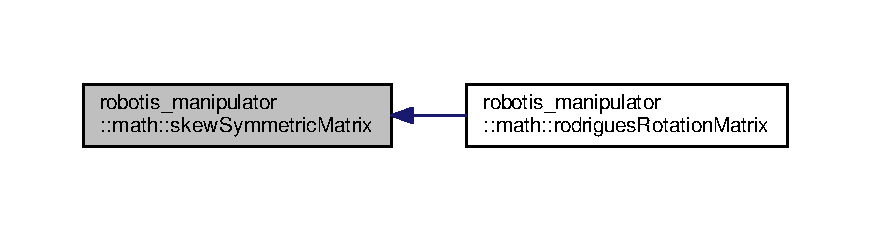
\includegraphics[width=350pt]{namespacerobotis__manipulator_1_1math_a03bf0fffc828339f2216fd4a98a32923_icgraph}
\end{center}
\end{figure}


\index{robotis\+\_\+manipulator\+::math@{robotis\+\_\+manipulator\+::math}!vector3@{vector3}}
\index{vector3@{vector3}!robotis\+\_\+manipulator\+::math@{robotis\+\_\+manipulator\+::math}}
\subsubsection[{\texorpdfstring{vector3(double v1, double v2, double v3)}{vector3(double v1, double v2, double v3)}}]{\setlength{\rightskip}{0pt plus 5cm}Eigen\+::\+Vector3d robotis\+\_\+manipulator\+::math\+::vector3 (
\begin{DoxyParamCaption}
\item[{double}]{v1, }
\item[{double}]{v2, }
\item[{double}]{v3}
\end{DoxyParamCaption}
)}\hypertarget{namespacerobotis__manipulator_1_1math_a057ca65131575b85aec169f3a50ed796}{}\label{namespacerobotis__manipulator_1_1math_a057ca65131575b85aec169f3a50ed796}


vector3 


\begin{DoxyParams}{Parameters}
{\em v1} & \\
\hline
{\em v2} & \\
\hline
{\em v3} & \\
\hline
\end{DoxyParams}
\begin{DoxyReturn}{Returns}

\end{DoxyReturn}


Definition at line 31 of file robotis\+\_\+manipulator\+\_\+math.\+cpp.


\begin{DoxyCode}
32 \{
33   Eigen::Vector3d temp;
34   temp << v1, v2, v3;
35   \textcolor{keywordflow}{return} temp;
36 \}
\end{DoxyCode}

\chapter{Class Documentation}
\hypertarget{structrobotis__manipulator_1_1_chaining_name}{}\section{robotis\+\_\+manipulator\+:\+:Chaining\+Name Struct Reference}
\label{structrobotis__manipulator_1_1_chaining_name}\index{robotis\+\_\+manipulator\+::\+Chaining\+Name@{robotis\+\_\+manipulator\+::\+Chaining\+Name}}


{\ttfamily \#include $<$robotis\+\_\+manipulator\+\_\+common.\+h$>$}



Collaboration diagram for robotis\+\_\+manipulator\+:\+:Chaining\+Name\+:\nopagebreak
\begin{figure}[H]
\begin{center}
\leavevmode
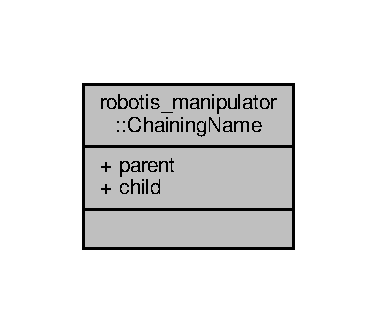
\includegraphics[width=181pt]{structrobotis__manipulator_1_1_chaining_name__coll__graph}
\end{center}
\end{figure}
\subsection*{Public Attributes}
\begin{DoxyCompactItemize}
\item 
\hyperlink{namespacerobotis__manipulator_a08c2d25e77a01ad75b9bb740f8ce4765}{Name} \hyperlink{structrobotis__manipulator_1_1_chaining_name_aa5e92a4939b2884e63bee3690f387627}{parent}
\item 
std\+::vector$<$ \hyperlink{namespacerobotis__manipulator_a08c2d25e77a01ad75b9bb740f8ce4765}{Name} $>$ \hyperlink{structrobotis__manipulator_1_1_chaining_name_a600be40420b93d2d8596d07d7e36fbf2}{child}
\end{DoxyCompactItemize}


\subsection{Detailed Description}


Definition at line 133 of file robotis\+\_\+manipulator\+\_\+common.\+h.



\subsection{Member Data Documentation}
\index{robotis\+\_\+manipulator\+::\+Chaining\+Name@{robotis\+\_\+manipulator\+::\+Chaining\+Name}!child@{child}}
\index{child@{child}!robotis\+\_\+manipulator\+::\+Chaining\+Name@{robotis\+\_\+manipulator\+::\+Chaining\+Name}}
\subsubsection[{\texorpdfstring{child}{child}}]{\setlength{\rightskip}{0pt plus 5cm}std\+::vector$<${\bf Name}$>$ robotis\+\_\+manipulator\+::\+Chaining\+Name\+::child}\hypertarget{structrobotis__manipulator_1_1_chaining_name_a600be40420b93d2d8596d07d7e36fbf2}{}\label{structrobotis__manipulator_1_1_chaining_name_a600be40420b93d2d8596d07d7e36fbf2}


Definition at line 136 of file robotis\+\_\+manipulator\+\_\+common.\+h.

\index{robotis\+\_\+manipulator\+::\+Chaining\+Name@{robotis\+\_\+manipulator\+::\+Chaining\+Name}!parent@{parent}}
\index{parent@{parent}!robotis\+\_\+manipulator\+::\+Chaining\+Name@{robotis\+\_\+manipulator\+::\+Chaining\+Name}}
\subsubsection[{\texorpdfstring{parent}{parent}}]{\setlength{\rightskip}{0pt plus 5cm}{\bf Name} robotis\+\_\+manipulator\+::\+Chaining\+Name\+::parent}\hypertarget{structrobotis__manipulator_1_1_chaining_name_aa5e92a4939b2884e63bee3690f387627}{}\label{structrobotis__manipulator_1_1_chaining_name_aa5e92a4939b2884e63bee3690f387627}


Definition at line 135 of file robotis\+\_\+manipulator\+\_\+common.\+h.



The documentation for this struct was generated from the following file\+:\begin{DoxyCompactItemize}
\item 
include/robotis\+\_\+manipulator/\hyperlink{robotis__manipulator__common_8h}{robotis\+\_\+manipulator\+\_\+common.\+h}\end{DoxyCompactItemize}

\hypertarget{structrobotis__manipulator_1_1_component}{}\section{robotis\+\_\+manipulator\+:\+:Component Struct Reference}
\label{structrobotis__manipulator_1_1_component}\index{robotis\+\_\+manipulator\+::\+Component@{robotis\+\_\+manipulator\+::\+Component}}


{\ttfamily \#include $<$robotis\+\_\+manipulator\+\_\+common.\+h$>$}



Collaboration diagram for robotis\+\_\+manipulator\+:\+:Component\+:\nopagebreak
\begin{figure}[H]
\begin{center}
\leavevmode
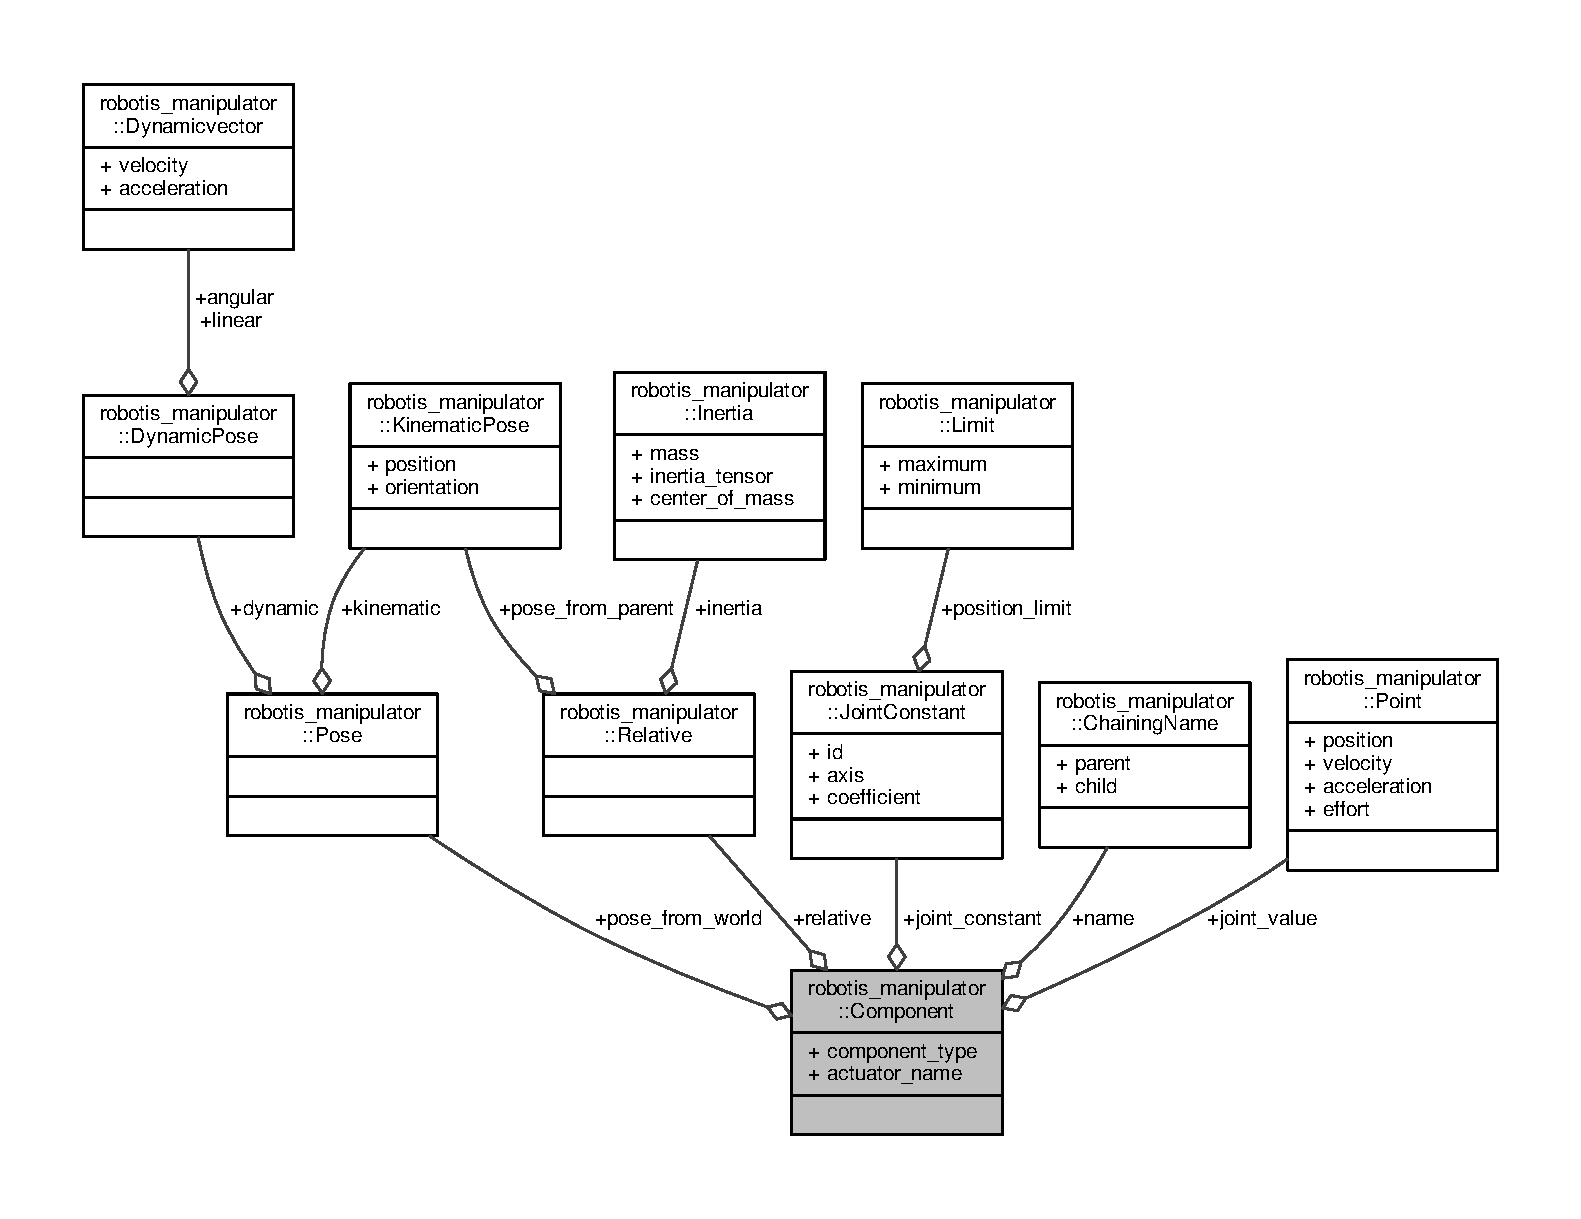
\includegraphics[width=350pt]{structrobotis__manipulator_1_1_component__coll__graph}
\end{center}
\end{figure}
\subsection*{Public Attributes}
\begin{DoxyCompactItemize}
\item 
\hyperlink{structrobotis__manipulator_1_1_chaining_name}{Chaining\+Name} \hyperlink{structrobotis__manipulator_1_1_component_a022aa062d295a3a6b5815a58b74e558f}{name}
\item 
\hyperlink{namespacerobotis__manipulator_a2bbf89d1c08dc1d9ff4e28beb939e382}{Component\+Type} \hyperlink{structrobotis__manipulator_1_1_component_ae597791dc579e168914ac36b66cf6172}{component\+\_\+type}
\item 
\hyperlink{structrobotis__manipulator_1_1_relative}{Relative} \hyperlink{structrobotis__manipulator_1_1_component_af1b86e91e0f92a214fa9e10464aba08f}{relative}
\item 
\hyperlink{structrobotis__manipulator_1_1_joint_constant}{Joint\+Constant} \hyperlink{structrobotis__manipulator_1_1_component_a39b967aba5061b7cd4e46c9a18d2e223}{joint\+\_\+constant}
\item 
\hyperlink{structrobotis__manipulator_1_1_pose}{Pose} \hyperlink{structrobotis__manipulator_1_1_component_a0b28dd5fe885ff8f07d75733d6e777fc}{pose\+\_\+from\+\_\+world}
\item 
\hyperlink{namespacerobotis__manipulator_aa0556c98c5294ccf3a96c2d0fe315e40}{Joint\+Value} \hyperlink{structrobotis__manipulator_1_1_component_a06de8406b177d397a1f998fdf9d67d95}{joint\+\_\+value}
\item 
\hyperlink{namespacerobotis__manipulator_a08c2d25e77a01ad75b9bb740f8ce4765}{Name} \hyperlink{structrobotis__manipulator_1_1_component_ac3407dba6190bf43305107fe7e443b6c}{actuator\+\_\+name}
\end{DoxyCompactItemize}


\subsection{Detailed Description}


Definition at line 160 of file robotis\+\_\+manipulator\+\_\+common.\+h.



\subsection{Member Data Documentation}
\index{robotis\+\_\+manipulator\+::\+Component@{robotis\+\_\+manipulator\+::\+Component}!actuator\+\_\+name@{actuator\+\_\+name}}
\index{actuator\+\_\+name@{actuator\+\_\+name}!robotis\+\_\+manipulator\+::\+Component@{robotis\+\_\+manipulator\+::\+Component}}
\subsubsection[{\texorpdfstring{actuator\+\_\+name}{actuator_name}}]{\setlength{\rightskip}{0pt plus 5cm}{\bf Name} robotis\+\_\+manipulator\+::\+Component\+::actuator\+\_\+name}\hypertarget{structrobotis__manipulator_1_1_component_ac3407dba6190bf43305107fe7e443b6c}{}\label{structrobotis__manipulator_1_1_component_ac3407dba6190bf43305107fe7e443b6c}


Definition at line 173 of file robotis\+\_\+manipulator\+\_\+common.\+h.

\index{robotis\+\_\+manipulator\+::\+Component@{robotis\+\_\+manipulator\+::\+Component}!component\+\_\+type@{component\+\_\+type}}
\index{component\+\_\+type@{component\+\_\+type}!robotis\+\_\+manipulator\+::\+Component@{robotis\+\_\+manipulator\+::\+Component}}
\subsubsection[{\texorpdfstring{component\+\_\+type}{component_type}}]{\setlength{\rightskip}{0pt plus 5cm}{\bf Component\+Type} robotis\+\_\+manipulator\+::\+Component\+::component\+\_\+type}\hypertarget{structrobotis__manipulator_1_1_component_ae597791dc579e168914ac36b66cf6172}{}\label{structrobotis__manipulator_1_1_component_ae597791dc579e168914ac36b66cf6172}


Definition at line 164 of file robotis\+\_\+manipulator\+\_\+common.\+h.

\index{robotis\+\_\+manipulator\+::\+Component@{robotis\+\_\+manipulator\+::\+Component}!joint\+\_\+constant@{joint\+\_\+constant}}
\index{joint\+\_\+constant@{joint\+\_\+constant}!robotis\+\_\+manipulator\+::\+Component@{robotis\+\_\+manipulator\+::\+Component}}
\subsubsection[{\texorpdfstring{joint\+\_\+constant}{joint_constant}}]{\setlength{\rightskip}{0pt plus 5cm}{\bf Joint\+Constant} robotis\+\_\+manipulator\+::\+Component\+::joint\+\_\+constant}\hypertarget{structrobotis__manipulator_1_1_component_a39b967aba5061b7cd4e46c9a18d2e223}{}\label{structrobotis__manipulator_1_1_component_a39b967aba5061b7cd4e46c9a18d2e223}


Definition at line 166 of file robotis\+\_\+manipulator\+\_\+common.\+h.

\index{robotis\+\_\+manipulator\+::\+Component@{robotis\+\_\+manipulator\+::\+Component}!joint\+\_\+value@{joint\+\_\+value}}
\index{joint\+\_\+value@{joint\+\_\+value}!robotis\+\_\+manipulator\+::\+Component@{robotis\+\_\+manipulator\+::\+Component}}
\subsubsection[{\texorpdfstring{joint\+\_\+value}{joint_value}}]{\setlength{\rightskip}{0pt plus 5cm}{\bf Joint\+Value} robotis\+\_\+manipulator\+::\+Component\+::joint\+\_\+value}\hypertarget{structrobotis__manipulator_1_1_component_a06de8406b177d397a1f998fdf9d67d95}{}\label{structrobotis__manipulator_1_1_component_a06de8406b177d397a1f998fdf9d67d95}


Definition at line 170 of file robotis\+\_\+manipulator\+\_\+common.\+h.

\index{robotis\+\_\+manipulator\+::\+Component@{robotis\+\_\+manipulator\+::\+Component}!name@{name}}
\index{name@{name}!robotis\+\_\+manipulator\+::\+Component@{robotis\+\_\+manipulator\+::\+Component}}
\subsubsection[{\texorpdfstring{name}{name}}]{\setlength{\rightskip}{0pt plus 5cm}{\bf Chaining\+Name} robotis\+\_\+manipulator\+::\+Component\+::name}\hypertarget{structrobotis__manipulator_1_1_component_a022aa062d295a3a6b5815a58b74e558f}{}\label{structrobotis__manipulator_1_1_component_a022aa062d295a3a6b5815a58b74e558f}


Definition at line 163 of file robotis\+\_\+manipulator\+\_\+common.\+h.

\index{robotis\+\_\+manipulator\+::\+Component@{robotis\+\_\+manipulator\+::\+Component}!pose\+\_\+from\+\_\+world@{pose\+\_\+from\+\_\+world}}
\index{pose\+\_\+from\+\_\+world@{pose\+\_\+from\+\_\+world}!robotis\+\_\+manipulator\+::\+Component@{robotis\+\_\+manipulator\+::\+Component}}
\subsubsection[{\texorpdfstring{pose\+\_\+from\+\_\+world}{pose_from_world}}]{\setlength{\rightskip}{0pt plus 5cm}{\bf Pose} robotis\+\_\+manipulator\+::\+Component\+::pose\+\_\+from\+\_\+world}\hypertarget{structrobotis__manipulator_1_1_component_a0b28dd5fe885ff8f07d75733d6e777fc}{}\label{structrobotis__manipulator_1_1_component_a0b28dd5fe885ff8f07d75733d6e777fc}


Definition at line 169 of file robotis\+\_\+manipulator\+\_\+common.\+h.

\index{robotis\+\_\+manipulator\+::\+Component@{robotis\+\_\+manipulator\+::\+Component}!relative@{relative}}
\index{relative@{relative}!robotis\+\_\+manipulator\+::\+Component@{robotis\+\_\+manipulator\+::\+Component}}
\subsubsection[{\texorpdfstring{relative}{relative}}]{\setlength{\rightskip}{0pt plus 5cm}{\bf Relative} robotis\+\_\+manipulator\+::\+Component\+::relative}\hypertarget{structrobotis__manipulator_1_1_component_af1b86e91e0f92a214fa9e10464aba08f}{}\label{structrobotis__manipulator_1_1_component_af1b86e91e0f92a214fa9e10464aba08f}


Definition at line 165 of file robotis\+\_\+manipulator\+\_\+common.\+h.



The documentation for this struct was generated from the following file\+:\begin{DoxyCompactItemize}
\item 
include/robotis\+\_\+manipulator/\hyperlink{robotis__manipulator__common_8h}{robotis\+\_\+manipulator\+\_\+common.\+h}\end{DoxyCompactItemize}

\hypertarget{classrobotis__manipulator_1_1_custom_joint_trajectory}{}\section{robotis\+\_\+manipulator\+:\+:Custom\+Joint\+Trajectory Class Reference}
\label{classrobotis__manipulator_1_1_custom_joint_trajectory}\index{robotis\+\_\+manipulator\+::\+Custom\+Joint\+Trajectory@{robotis\+\_\+manipulator\+::\+Custom\+Joint\+Trajectory}}


The \hyperlink{classrobotis__manipulator_1_1_custom_joint_trajectory}{Custom\+Joint\+Trajectory} class.  




{\ttfamily \#include $<$robotis\+\_\+manipulator\+\_\+manager.\+h$>$}



Collaboration diagram for robotis\+\_\+manipulator\+:\+:Custom\+Joint\+Trajectory\+:\nopagebreak
\begin{figure}[H]
\begin{center}
\leavevmode
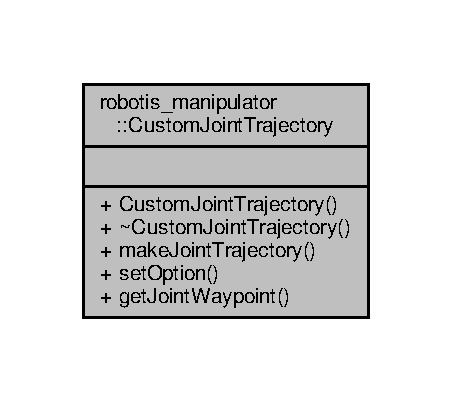
\includegraphics[width=217pt]{classrobotis__manipulator_1_1_custom_joint_trajectory__coll__graph}
\end{center}
\end{figure}
\subsection*{Public Member Functions}
\begin{DoxyCompactItemize}
\item 
\hyperlink{classrobotis__manipulator_1_1_custom_joint_trajectory_a68daf69c70b60f58a30b235618448bd6}{Custom\+Joint\+Trajectory} ()
\item 
virtual \hyperlink{classrobotis__manipulator_1_1_custom_joint_trajectory_a0b26437cc90db37b0054f57ce4619fc3}{$\sim$\+Custom\+Joint\+Trajectory} ()
\item 
virtual void \hyperlink{classrobotis__manipulator_1_1_custom_joint_trajectory_af407a0f777289295dd1bbae692d5761a}{make\+Joint\+Trajectory} (double move\+\_\+time, \hyperlink{namespacerobotis__manipulator_a4456fd8b14e1f6b7733a77837dfe9339}{Joint\+Waypoint} start, const void $\ast$arg)=0
\begin{DoxyCompactList}\small\item\em make\+Joint\+Trajectory \end{DoxyCompactList}\item 
virtual void \hyperlink{classrobotis__manipulator_1_1_custom_joint_trajectory_a3e6eb8b2ad0c0b9647864e377b41d099}{set\+Option} (const void $\ast$arg)=0
\begin{DoxyCompactList}\small\item\em set\+Option \end{DoxyCompactList}\item 
virtual \hyperlink{namespacerobotis__manipulator_a4456fd8b14e1f6b7733a77837dfe9339}{Joint\+Waypoint} \hyperlink{classrobotis__manipulator_1_1_custom_joint_trajectory_aa8f8cae5e28d0b4400d4ba9af9a3c396}{get\+Joint\+Waypoint} (double tick)=0
\begin{DoxyCompactList}\small\item\em get\+Joint\+Waypoint \end{DoxyCompactList}\end{DoxyCompactItemize}


\subsection{Detailed Description}
The \hyperlink{classrobotis__manipulator_1_1_custom_joint_trajectory}{Custom\+Joint\+Trajectory} class. 

Definition at line 214 of file robotis\+\_\+manipulator\+\_\+manager.\+h.



\subsection{Constructor \& Destructor Documentation}
\index{robotis\+\_\+manipulator\+::\+Custom\+Joint\+Trajectory@{robotis\+\_\+manipulator\+::\+Custom\+Joint\+Trajectory}!Custom\+Joint\+Trajectory@{Custom\+Joint\+Trajectory}}
\index{Custom\+Joint\+Trajectory@{Custom\+Joint\+Trajectory}!robotis\+\_\+manipulator\+::\+Custom\+Joint\+Trajectory@{robotis\+\_\+manipulator\+::\+Custom\+Joint\+Trajectory}}
\subsubsection[{\texorpdfstring{Custom\+Joint\+Trajectory()}{CustomJointTrajectory()}}]{\setlength{\rightskip}{0pt plus 5cm}robotis\+\_\+manipulator\+::\+Custom\+Joint\+Trajectory\+::\+Custom\+Joint\+Trajectory (
\begin{DoxyParamCaption}
{}
\end{DoxyParamCaption}
)\hspace{0.3cm}{\ttfamily [inline]}}\hypertarget{classrobotis__manipulator_1_1_custom_joint_trajectory_a68daf69c70b60f58a30b235618448bd6}{}\label{classrobotis__manipulator_1_1_custom_joint_trajectory_a68daf69c70b60f58a30b235618448bd6}


Definition at line 217 of file robotis\+\_\+manipulator\+\_\+manager.\+h.


\begin{DoxyCode}
217 \{\}
\end{DoxyCode}
\index{robotis\+\_\+manipulator\+::\+Custom\+Joint\+Trajectory@{robotis\+\_\+manipulator\+::\+Custom\+Joint\+Trajectory}!````~Custom\+Joint\+Trajectory@{$\sim$\+Custom\+Joint\+Trajectory}}
\index{````~Custom\+Joint\+Trajectory@{$\sim$\+Custom\+Joint\+Trajectory}!robotis\+\_\+manipulator\+::\+Custom\+Joint\+Trajectory@{robotis\+\_\+manipulator\+::\+Custom\+Joint\+Trajectory}}
\subsubsection[{\texorpdfstring{$\sim$\+Custom\+Joint\+Trajectory()}{~CustomJointTrajectory()}}]{\setlength{\rightskip}{0pt plus 5cm}virtual robotis\+\_\+manipulator\+::\+Custom\+Joint\+Trajectory\+::$\sim$\+Custom\+Joint\+Trajectory (
\begin{DoxyParamCaption}
{}
\end{DoxyParamCaption}
)\hspace{0.3cm}{\ttfamily [inline]}, {\ttfamily [virtual]}}\hypertarget{classrobotis__manipulator_1_1_custom_joint_trajectory_a0b26437cc90db37b0054f57ce4619fc3}{}\label{classrobotis__manipulator_1_1_custom_joint_trajectory_a0b26437cc90db37b0054f57ce4619fc3}


Definition at line 218 of file robotis\+\_\+manipulator\+\_\+manager.\+h.


\begin{DoxyCode}
218 \{\}
\end{DoxyCode}


Here is the call graph for this function\+:\nopagebreak
\begin{figure}[H]
\begin{center}
\leavevmode
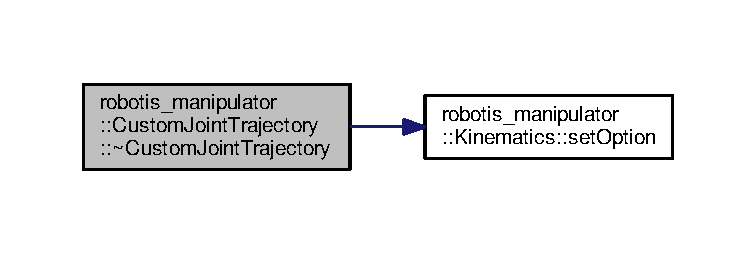
\includegraphics[width=350pt]{classrobotis__manipulator_1_1_custom_joint_trajectory_a0b26437cc90db37b0054f57ce4619fc3_cgraph}
\end{center}
\end{figure}




\subsection{Member Function Documentation}
\index{robotis\+\_\+manipulator\+::\+Custom\+Joint\+Trajectory@{robotis\+\_\+manipulator\+::\+Custom\+Joint\+Trajectory}!get\+Joint\+Waypoint@{get\+Joint\+Waypoint}}
\index{get\+Joint\+Waypoint@{get\+Joint\+Waypoint}!robotis\+\_\+manipulator\+::\+Custom\+Joint\+Trajectory@{robotis\+\_\+manipulator\+::\+Custom\+Joint\+Trajectory}}
\subsubsection[{\texorpdfstring{get\+Joint\+Waypoint(double tick)=0}{getJointWaypoint(double tick)=0}}]{\setlength{\rightskip}{0pt plus 5cm}virtual {\bf Joint\+Waypoint} robotis\+\_\+manipulator\+::\+Custom\+Joint\+Trajectory\+::get\+Joint\+Waypoint (
\begin{DoxyParamCaption}
\item[{double}]{tick}
\end{DoxyParamCaption}
)\hspace{0.3cm}{\ttfamily [pure virtual]}}\hypertarget{classrobotis__manipulator_1_1_custom_joint_trajectory_aa8f8cae5e28d0b4400d4ba9af9a3c396}{}\label{classrobotis__manipulator_1_1_custom_joint_trajectory_aa8f8cae5e28d0b4400d4ba9af9a3c396}


get\+Joint\+Waypoint 


\begin{DoxyParams}{Parameters}
{\em tick} & \\
\hline
\end{DoxyParams}
\begin{DoxyReturn}{Returns}

\end{DoxyReturn}
\index{robotis\+\_\+manipulator\+::\+Custom\+Joint\+Trajectory@{robotis\+\_\+manipulator\+::\+Custom\+Joint\+Trajectory}!make\+Joint\+Trajectory@{make\+Joint\+Trajectory}}
\index{make\+Joint\+Trajectory@{make\+Joint\+Trajectory}!robotis\+\_\+manipulator\+::\+Custom\+Joint\+Trajectory@{robotis\+\_\+manipulator\+::\+Custom\+Joint\+Trajectory}}
\subsubsection[{\texorpdfstring{make\+Joint\+Trajectory(double move\+\_\+time, Joint\+Waypoint start, const void $\ast$arg)=0}{makeJointTrajectory(double move_time, JointWaypoint start, const void *arg)=0}}]{\setlength{\rightskip}{0pt plus 5cm}virtual void robotis\+\_\+manipulator\+::\+Custom\+Joint\+Trajectory\+::make\+Joint\+Trajectory (
\begin{DoxyParamCaption}
\item[{double}]{move\+\_\+time, }
\item[{{\bf Joint\+Waypoint}}]{start, }
\item[{const void $\ast$}]{arg}
\end{DoxyParamCaption}
)\hspace{0.3cm}{\ttfamily [pure virtual]}}\hypertarget{classrobotis__manipulator_1_1_custom_joint_trajectory_af407a0f777289295dd1bbae692d5761a}{}\label{classrobotis__manipulator_1_1_custom_joint_trajectory_af407a0f777289295dd1bbae692d5761a}


make\+Joint\+Trajectory 


\begin{DoxyParams}{Parameters}
{\em move\+\_\+time} & \\
\hline
{\em start} & \\
\hline
{\em arg} & \\
\hline
\end{DoxyParams}
\index{robotis\+\_\+manipulator\+::\+Custom\+Joint\+Trajectory@{robotis\+\_\+manipulator\+::\+Custom\+Joint\+Trajectory}!set\+Option@{set\+Option}}
\index{set\+Option@{set\+Option}!robotis\+\_\+manipulator\+::\+Custom\+Joint\+Trajectory@{robotis\+\_\+manipulator\+::\+Custom\+Joint\+Trajectory}}
\subsubsection[{\texorpdfstring{set\+Option(const void $\ast$arg)=0}{setOption(const void *arg)=0}}]{\setlength{\rightskip}{0pt plus 5cm}virtual void robotis\+\_\+manipulator\+::\+Custom\+Joint\+Trajectory\+::set\+Option (
\begin{DoxyParamCaption}
\item[{const void $\ast$}]{arg}
\end{DoxyParamCaption}
)\hspace{0.3cm}{\ttfamily [pure virtual]}}\hypertarget{classrobotis__manipulator_1_1_custom_joint_trajectory_a3e6eb8b2ad0c0b9647864e377b41d099}{}\label{classrobotis__manipulator_1_1_custom_joint_trajectory_a3e6eb8b2ad0c0b9647864e377b41d099}


set\+Option 


\begin{DoxyParams}{Parameters}
{\em arg} & \\
\hline
\end{DoxyParams}


The documentation for this class was generated from the following file\+:\begin{DoxyCompactItemize}
\item 
include/robotis\+\_\+manipulator/\hyperlink{robotis__manipulator__manager_8h}{robotis\+\_\+manipulator\+\_\+manager.\+h}\end{DoxyCompactItemize}

\hypertarget{classrobotis__manipulator_1_1_custom_task_trajectory}{}\section{robotis\+\_\+manipulator\+:\+:Custom\+Task\+Trajectory Class Reference}
\label{classrobotis__manipulator_1_1_custom_task_trajectory}\index{robotis\+\_\+manipulator\+::\+Custom\+Task\+Trajectory@{robotis\+\_\+manipulator\+::\+Custom\+Task\+Trajectory}}


The \hyperlink{classrobotis__manipulator_1_1_custom_task_trajectory}{Custom\+Task\+Trajectory} class.  




{\ttfamily \#include $<$robotis\+\_\+manipulator\+\_\+manager.\+h$>$}



Collaboration diagram for robotis\+\_\+manipulator\+:\+:Custom\+Task\+Trajectory\+:\nopagebreak
\begin{figure}[H]
\begin{center}
\leavevmode
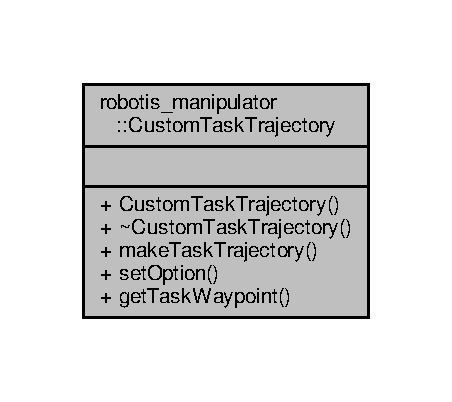
\includegraphics[width=217pt]{classrobotis__manipulator_1_1_custom_task_trajectory__coll__graph}
\end{center}
\end{figure}
\subsection*{Public Member Functions}
\begin{DoxyCompactItemize}
\item 
\hyperlink{classrobotis__manipulator_1_1_custom_task_trajectory_ac2d9f3dc73a9b355d967835d5aafc274}{Custom\+Task\+Trajectory} ()
\item 
virtual \hyperlink{classrobotis__manipulator_1_1_custom_task_trajectory_a9895c8d695786bdf868de651d5aa170d}{$\sim$\+Custom\+Task\+Trajectory} ()
\item 
virtual void \hyperlink{classrobotis__manipulator_1_1_custom_task_trajectory_a06278d45f1b80a9994617c61daefac99}{make\+Task\+Trajectory} (double move\+\_\+time, \hyperlink{namespacerobotis__manipulator_a440e2d88ec85fdee394e540dc6024c3e}{Task\+Waypoint} start, const void $\ast$arg)=0
\begin{DoxyCompactList}\small\item\em make\+Task\+Trajectory \end{DoxyCompactList}\item 
virtual void \hyperlink{classrobotis__manipulator_1_1_custom_task_trajectory_a027ae37e3adbdfe634442351240619f1}{set\+Option} (const void $\ast$arg)=0
\begin{DoxyCompactList}\small\item\em set\+Option \end{DoxyCompactList}\item 
virtual \hyperlink{namespacerobotis__manipulator_a440e2d88ec85fdee394e540dc6024c3e}{Task\+Waypoint} \hyperlink{classrobotis__manipulator_1_1_custom_task_trajectory_aa304eee6a768c221750e88faaa3689b8}{get\+Task\+Waypoint} (double tick)=0
\begin{DoxyCompactList}\small\item\em get\+Task\+Waypoint \end{DoxyCompactList}\end{DoxyCompactItemize}


\subsection{Detailed Description}
The \hyperlink{classrobotis__manipulator_1_1_custom_task_trajectory}{Custom\+Task\+Trajectory} class. 

Definition at line 243 of file robotis\+\_\+manipulator\+\_\+manager.\+h.



\subsection{Constructor \& Destructor Documentation}
\index{robotis\+\_\+manipulator\+::\+Custom\+Task\+Trajectory@{robotis\+\_\+manipulator\+::\+Custom\+Task\+Trajectory}!Custom\+Task\+Trajectory@{Custom\+Task\+Trajectory}}
\index{Custom\+Task\+Trajectory@{Custom\+Task\+Trajectory}!robotis\+\_\+manipulator\+::\+Custom\+Task\+Trajectory@{robotis\+\_\+manipulator\+::\+Custom\+Task\+Trajectory}}
\subsubsection[{\texorpdfstring{Custom\+Task\+Trajectory()}{CustomTaskTrajectory()}}]{\setlength{\rightskip}{0pt plus 5cm}robotis\+\_\+manipulator\+::\+Custom\+Task\+Trajectory\+::\+Custom\+Task\+Trajectory (
\begin{DoxyParamCaption}
{}
\end{DoxyParamCaption}
)\hspace{0.3cm}{\ttfamily [inline]}}\hypertarget{classrobotis__manipulator_1_1_custom_task_trajectory_ac2d9f3dc73a9b355d967835d5aafc274}{}\label{classrobotis__manipulator_1_1_custom_task_trajectory_ac2d9f3dc73a9b355d967835d5aafc274}


Definition at line 246 of file robotis\+\_\+manipulator\+\_\+manager.\+h.


\begin{DoxyCode}
246 \{\}
\end{DoxyCode}
\index{robotis\+\_\+manipulator\+::\+Custom\+Task\+Trajectory@{robotis\+\_\+manipulator\+::\+Custom\+Task\+Trajectory}!````~Custom\+Task\+Trajectory@{$\sim$\+Custom\+Task\+Trajectory}}
\index{````~Custom\+Task\+Trajectory@{$\sim$\+Custom\+Task\+Trajectory}!robotis\+\_\+manipulator\+::\+Custom\+Task\+Trajectory@{robotis\+\_\+manipulator\+::\+Custom\+Task\+Trajectory}}
\subsubsection[{\texorpdfstring{$\sim$\+Custom\+Task\+Trajectory()}{~CustomTaskTrajectory()}}]{\setlength{\rightskip}{0pt plus 5cm}virtual robotis\+\_\+manipulator\+::\+Custom\+Task\+Trajectory\+::$\sim$\+Custom\+Task\+Trajectory (
\begin{DoxyParamCaption}
{}
\end{DoxyParamCaption}
)\hspace{0.3cm}{\ttfamily [inline]}, {\ttfamily [virtual]}}\hypertarget{classrobotis__manipulator_1_1_custom_task_trajectory_a9895c8d695786bdf868de651d5aa170d}{}\label{classrobotis__manipulator_1_1_custom_task_trajectory_a9895c8d695786bdf868de651d5aa170d}


Definition at line 247 of file robotis\+\_\+manipulator\+\_\+manager.\+h.


\begin{DoxyCode}
247 \{\}
\end{DoxyCode}


Here is the call graph for this function\+:\nopagebreak
\begin{figure}[H]
\begin{center}
\leavevmode
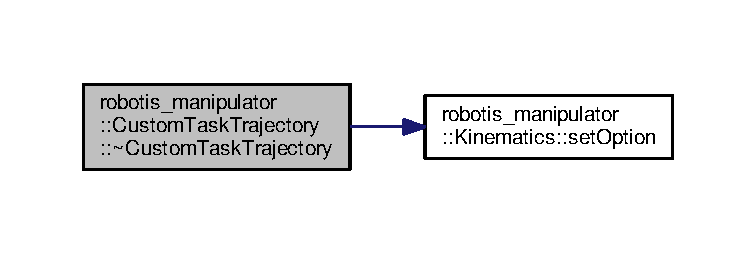
\includegraphics[width=350pt]{classrobotis__manipulator_1_1_custom_task_trajectory_a9895c8d695786bdf868de651d5aa170d_cgraph}
\end{center}
\end{figure}




\subsection{Member Function Documentation}
\index{robotis\+\_\+manipulator\+::\+Custom\+Task\+Trajectory@{robotis\+\_\+manipulator\+::\+Custom\+Task\+Trajectory}!get\+Task\+Waypoint@{get\+Task\+Waypoint}}
\index{get\+Task\+Waypoint@{get\+Task\+Waypoint}!robotis\+\_\+manipulator\+::\+Custom\+Task\+Trajectory@{robotis\+\_\+manipulator\+::\+Custom\+Task\+Trajectory}}
\subsubsection[{\texorpdfstring{get\+Task\+Waypoint(double tick)=0}{getTaskWaypoint(double tick)=0}}]{\setlength{\rightskip}{0pt plus 5cm}virtual {\bf Task\+Waypoint} robotis\+\_\+manipulator\+::\+Custom\+Task\+Trajectory\+::get\+Task\+Waypoint (
\begin{DoxyParamCaption}
\item[{double}]{tick}
\end{DoxyParamCaption}
)\hspace{0.3cm}{\ttfamily [pure virtual]}}\hypertarget{classrobotis__manipulator_1_1_custom_task_trajectory_aa304eee6a768c221750e88faaa3689b8}{}\label{classrobotis__manipulator_1_1_custom_task_trajectory_aa304eee6a768c221750e88faaa3689b8}


get\+Task\+Waypoint 


\begin{DoxyParams}{Parameters}
{\em tick} & \\
\hline
\end{DoxyParams}
\begin{DoxyReturn}{Returns}

\end{DoxyReturn}
\index{robotis\+\_\+manipulator\+::\+Custom\+Task\+Trajectory@{robotis\+\_\+manipulator\+::\+Custom\+Task\+Trajectory}!make\+Task\+Trajectory@{make\+Task\+Trajectory}}
\index{make\+Task\+Trajectory@{make\+Task\+Trajectory}!robotis\+\_\+manipulator\+::\+Custom\+Task\+Trajectory@{robotis\+\_\+manipulator\+::\+Custom\+Task\+Trajectory}}
\subsubsection[{\texorpdfstring{make\+Task\+Trajectory(double move\+\_\+time, Task\+Waypoint start, const void $\ast$arg)=0}{makeTaskTrajectory(double move_time, TaskWaypoint start, const void *arg)=0}}]{\setlength{\rightskip}{0pt plus 5cm}virtual void robotis\+\_\+manipulator\+::\+Custom\+Task\+Trajectory\+::make\+Task\+Trajectory (
\begin{DoxyParamCaption}
\item[{double}]{move\+\_\+time, }
\item[{{\bf Task\+Waypoint}}]{start, }
\item[{const void $\ast$}]{arg}
\end{DoxyParamCaption}
)\hspace{0.3cm}{\ttfamily [pure virtual]}}\hypertarget{classrobotis__manipulator_1_1_custom_task_trajectory_a06278d45f1b80a9994617c61daefac99}{}\label{classrobotis__manipulator_1_1_custom_task_trajectory_a06278d45f1b80a9994617c61daefac99}


make\+Task\+Trajectory 


\begin{DoxyParams}{Parameters}
{\em move\+\_\+time} & \\
\hline
{\em start} & \\
\hline
{\em arg} & \\
\hline
\end{DoxyParams}
\index{robotis\+\_\+manipulator\+::\+Custom\+Task\+Trajectory@{robotis\+\_\+manipulator\+::\+Custom\+Task\+Trajectory}!set\+Option@{set\+Option}}
\index{set\+Option@{set\+Option}!robotis\+\_\+manipulator\+::\+Custom\+Task\+Trajectory@{robotis\+\_\+manipulator\+::\+Custom\+Task\+Trajectory}}
\subsubsection[{\texorpdfstring{set\+Option(const void $\ast$arg)=0}{setOption(const void *arg)=0}}]{\setlength{\rightskip}{0pt plus 5cm}virtual void robotis\+\_\+manipulator\+::\+Custom\+Task\+Trajectory\+::set\+Option (
\begin{DoxyParamCaption}
\item[{const void $\ast$}]{arg}
\end{DoxyParamCaption}
)\hspace{0.3cm}{\ttfamily [pure virtual]}}\hypertarget{classrobotis__manipulator_1_1_custom_task_trajectory_a027ae37e3adbdfe634442351240619f1}{}\label{classrobotis__manipulator_1_1_custom_task_trajectory_a027ae37e3adbdfe634442351240619f1}


set\+Option 


\begin{DoxyParams}{Parameters}
{\em arg} & \\
\hline
\end{DoxyParams}


The documentation for this class was generated from the following file\+:\begin{DoxyCompactItemize}
\item 
include/robotis\+\_\+manipulator/\hyperlink{robotis__manipulator__manager_8h}{robotis\+\_\+manipulator\+\_\+manager.\+h}\end{DoxyCompactItemize}

\hypertarget{structrobotis__manipulator_1_1_dynamic_pose}{}\section{robotis\+\_\+manipulator\+:\+:Dynamic\+Pose Struct Reference}
\label{structrobotis__manipulator_1_1_dynamic_pose}\index{robotis\+\_\+manipulator\+::\+Dynamic\+Pose@{robotis\+\_\+manipulator\+::\+Dynamic\+Pose}}


{\ttfamily \#include $<$robotis\+\_\+manipulator\+\_\+common.\+h$>$}



Collaboration diagram for robotis\+\_\+manipulator\+:\+:Dynamic\+Pose\+:\nopagebreak
\begin{figure}[H]
\begin{center}
\leavevmode
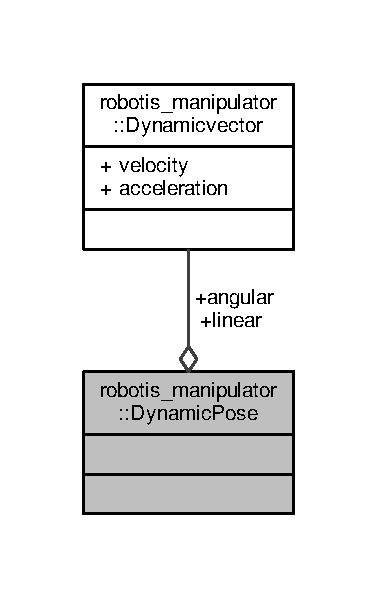
\includegraphics[width=181pt]{structrobotis__manipulator_1_1_dynamic_pose__coll__graph}
\end{center}
\end{figure}
\subsection*{Public Attributes}
\begin{DoxyCompactItemize}
\item 
\hyperlink{structrobotis__manipulator_1_1_dynamicvector}{Dynamicvector} \hyperlink{structrobotis__manipulator_1_1_dynamic_pose_a45f314d8e2d3f78a4bc9c2aa72f0badc}{linear}
\item 
\hyperlink{structrobotis__manipulator_1_1_dynamicvector}{Dynamicvector} \hyperlink{structrobotis__manipulator_1_1_dynamic_pose_a424459b0d1108f1e65594f5d193cbae6}{angular}
\end{DoxyCompactItemize}


\subsection{Detailed Description}


Definition at line 63 of file robotis\+\_\+manipulator\+\_\+common.\+h.



\subsection{Member Data Documentation}
\index{robotis\+\_\+manipulator\+::\+Dynamic\+Pose@{robotis\+\_\+manipulator\+::\+Dynamic\+Pose}!angular@{angular}}
\index{angular@{angular}!robotis\+\_\+manipulator\+::\+Dynamic\+Pose@{robotis\+\_\+manipulator\+::\+Dynamic\+Pose}}
\subsubsection[{\texorpdfstring{angular}{angular}}]{\setlength{\rightskip}{0pt plus 5cm}{\bf Dynamicvector} robotis\+\_\+manipulator\+::\+Dynamic\+Pose\+::angular}\hypertarget{structrobotis__manipulator_1_1_dynamic_pose_a424459b0d1108f1e65594f5d193cbae6}{}\label{structrobotis__manipulator_1_1_dynamic_pose_a424459b0d1108f1e65594f5d193cbae6}


Definition at line 66 of file robotis\+\_\+manipulator\+\_\+common.\+h.

\index{robotis\+\_\+manipulator\+::\+Dynamic\+Pose@{robotis\+\_\+manipulator\+::\+Dynamic\+Pose}!linear@{linear}}
\index{linear@{linear}!robotis\+\_\+manipulator\+::\+Dynamic\+Pose@{robotis\+\_\+manipulator\+::\+Dynamic\+Pose}}
\subsubsection[{\texorpdfstring{linear}{linear}}]{\setlength{\rightskip}{0pt plus 5cm}{\bf Dynamicvector} robotis\+\_\+manipulator\+::\+Dynamic\+Pose\+::linear}\hypertarget{structrobotis__manipulator_1_1_dynamic_pose_a45f314d8e2d3f78a4bc9c2aa72f0badc}{}\label{structrobotis__manipulator_1_1_dynamic_pose_a45f314d8e2d3f78a4bc9c2aa72f0badc}


Definition at line 65 of file robotis\+\_\+manipulator\+\_\+common.\+h.



The documentation for this struct was generated from the following file\+:\begin{DoxyCompactItemize}
\item 
include/robotis\+\_\+manipulator/\hyperlink{robotis__manipulator__common_8h}{robotis\+\_\+manipulator\+\_\+common.\+h}\end{DoxyCompactItemize}

\hypertarget{structrobotis__manipulator_1_1_dynamicvector}{}\section{robotis\+\_\+manipulator\+:\+:Dynamicvector Struct Reference}
\label{structrobotis__manipulator_1_1_dynamicvector}\index{robotis\+\_\+manipulator\+::\+Dynamicvector@{robotis\+\_\+manipulator\+::\+Dynamicvector}}


{\ttfamily \#include $<$robotis\+\_\+manipulator\+\_\+common.\+h$>$}



Collaboration diagram for robotis\+\_\+manipulator\+:\+:Dynamicvector\+:\nopagebreak
\begin{figure}[H]
\begin{center}
\leavevmode
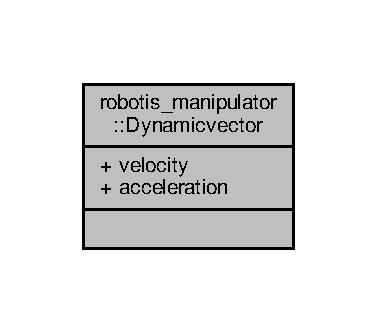
\includegraphics[width=181pt]{structrobotis__manipulator_1_1_dynamicvector__coll__graph}
\end{center}
\end{figure}
\subsection*{Public Attributes}
\begin{DoxyCompactItemize}
\item 
Eigen\+::\+Vector3d \hyperlink{structrobotis__manipulator_1_1_dynamicvector_a6bbccf8316887a8da3cd6aa065f3beac}{velocity}
\item 
Eigen\+::\+Vector3d \hyperlink{structrobotis__manipulator_1_1_dynamicvector_afc83eba2d67af4c23150a08824f0f01e}{acceleration}
\end{DoxyCompactItemize}


\subsection{Detailed Description}


Definition at line 57 of file robotis\+\_\+manipulator\+\_\+common.\+h.



\subsection{Member Data Documentation}
\index{robotis\+\_\+manipulator\+::\+Dynamicvector@{robotis\+\_\+manipulator\+::\+Dynamicvector}!acceleration@{acceleration}}
\index{acceleration@{acceleration}!robotis\+\_\+manipulator\+::\+Dynamicvector@{robotis\+\_\+manipulator\+::\+Dynamicvector}}
\subsubsection[{\texorpdfstring{acceleration}{acceleration}}]{\setlength{\rightskip}{0pt plus 5cm}Eigen\+::\+Vector3d robotis\+\_\+manipulator\+::\+Dynamicvector\+::acceleration}\hypertarget{structrobotis__manipulator_1_1_dynamicvector_afc83eba2d67af4c23150a08824f0f01e}{}\label{structrobotis__manipulator_1_1_dynamicvector_afc83eba2d67af4c23150a08824f0f01e}


Definition at line 60 of file robotis\+\_\+manipulator\+\_\+common.\+h.

\index{robotis\+\_\+manipulator\+::\+Dynamicvector@{robotis\+\_\+manipulator\+::\+Dynamicvector}!velocity@{velocity}}
\index{velocity@{velocity}!robotis\+\_\+manipulator\+::\+Dynamicvector@{robotis\+\_\+manipulator\+::\+Dynamicvector}}
\subsubsection[{\texorpdfstring{velocity}{velocity}}]{\setlength{\rightskip}{0pt plus 5cm}Eigen\+::\+Vector3d robotis\+\_\+manipulator\+::\+Dynamicvector\+::velocity}\hypertarget{structrobotis__manipulator_1_1_dynamicvector_a6bbccf8316887a8da3cd6aa065f3beac}{}\label{structrobotis__manipulator_1_1_dynamicvector_a6bbccf8316887a8da3cd6aa065f3beac}


Definition at line 59 of file robotis\+\_\+manipulator\+\_\+common.\+h.



The documentation for this struct was generated from the following file\+:\begin{DoxyCompactItemize}
\item 
include/robotis\+\_\+manipulator/\hyperlink{robotis__manipulator__common_8h}{robotis\+\_\+manipulator\+\_\+common.\+h}\end{DoxyCompactItemize}

\hypertarget{structrobotis__manipulator_1_1_inertia}{}\section{robotis\+\_\+manipulator\+:\+:Inertia Struct Reference}
\label{structrobotis__manipulator_1_1_inertia}\index{robotis\+\_\+manipulator\+::\+Inertia@{robotis\+\_\+manipulator\+::\+Inertia}}


{\ttfamily \#include $<$robotis\+\_\+manipulator\+\_\+common.\+h$>$}



Collaboration diagram for robotis\+\_\+manipulator\+:\+:Inertia\+:\nopagebreak
\begin{figure}[H]
\begin{center}
\leavevmode
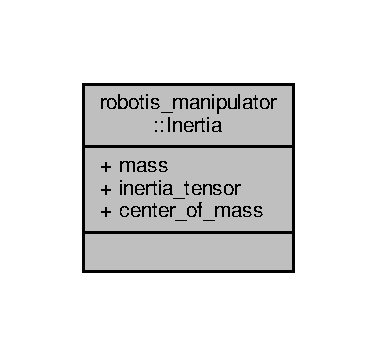
\includegraphics[width=181pt]{structrobotis__manipulator_1_1_inertia__coll__graph}
\end{center}
\end{figure}
\subsection*{Public Attributes}
\begin{DoxyCompactItemize}
\item 
double \hyperlink{structrobotis__manipulator_1_1_inertia_a8e25738415288febca11a62124736bab}{mass}
\item 
Eigen\+::\+Matrix3d \hyperlink{structrobotis__manipulator_1_1_inertia_a61b16b0ad0ac7366fe046b946c04c97e}{inertia\+\_\+tensor}
\item 
Eigen\+::\+Vector3d \hyperlink{structrobotis__manipulator_1_1_inertia_a8d7158602370b1abf0b690a6483376b7}{center\+\_\+of\+\_\+mass}
\end{DoxyCompactItemize}


\subsection{Detailed Description}


Definition at line 69 of file robotis\+\_\+manipulator\+\_\+common.\+h.



\subsection{Member Data Documentation}
\index{robotis\+\_\+manipulator\+::\+Inertia@{robotis\+\_\+manipulator\+::\+Inertia}!center\+\_\+of\+\_\+mass@{center\+\_\+of\+\_\+mass}}
\index{center\+\_\+of\+\_\+mass@{center\+\_\+of\+\_\+mass}!robotis\+\_\+manipulator\+::\+Inertia@{robotis\+\_\+manipulator\+::\+Inertia}}
\subsubsection[{\texorpdfstring{center\+\_\+of\+\_\+mass}{center_of_mass}}]{\setlength{\rightskip}{0pt plus 5cm}Eigen\+::\+Vector3d robotis\+\_\+manipulator\+::\+Inertia\+::center\+\_\+of\+\_\+mass}\hypertarget{structrobotis__manipulator_1_1_inertia_a8d7158602370b1abf0b690a6483376b7}{}\label{structrobotis__manipulator_1_1_inertia_a8d7158602370b1abf0b690a6483376b7}


Definition at line 73 of file robotis\+\_\+manipulator\+\_\+common.\+h.

\index{robotis\+\_\+manipulator\+::\+Inertia@{robotis\+\_\+manipulator\+::\+Inertia}!inertia\+\_\+tensor@{inertia\+\_\+tensor}}
\index{inertia\+\_\+tensor@{inertia\+\_\+tensor}!robotis\+\_\+manipulator\+::\+Inertia@{robotis\+\_\+manipulator\+::\+Inertia}}
\subsubsection[{\texorpdfstring{inertia\+\_\+tensor}{inertia_tensor}}]{\setlength{\rightskip}{0pt plus 5cm}Eigen\+::\+Matrix3d robotis\+\_\+manipulator\+::\+Inertia\+::inertia\+\_\+tensor}\hypertarget{structrobotis__manipulator_1_1_inertia_a61b16b0ad0ac7366fe046b946c04c97e}{}\label{structrobotis__manipulator_1_1_inertia_a61b16b0ad0ac7366fe046b946c04c97e}


Definition at line 72 of file robotis\+\_\+manipulator\+\_\+common.\+h.

\index{robotis\+\_\+manipulator\+::\+Inertia@{robotis\+\_\+manipulator\+::\+Inertia}!mass@{mass}}
\index{mass@{mass}!robotis\+\_\+manipulator\+::\+Inertia@{robotis\+\_\+manipulator\+::\+Inertia}}
\subsubsection[{\texorpdfstring{mass}{mass}}]{\setlength{\rightskip}{0pt plus 5cm}double robotis\+\_\+manipulator\+::\+Inertia\+::mass}\hypertarget{structrobotis__manipulator_1_1_inertia_a8e25738415288febca11a62124736bab}{}\label{structrobotis__manipulator_1_1_inertia_a8e25738415288febca11a62124736bab}


Definition at line 71 of file robotis\+\_\+manipulator\+\_\+common.\+h.



The documentation for this struct was generated from the following file\+:\begin{DoxyCompactItemize}
\item 
include/robotis\+\_\+manipulator/\hyperlink{robotis__manipulator__common_8h}{robotis\+\_\+manipulator\+\_\+common.\+h}\end{DoxyCompactItemize}

\hypertarget{classrobotis__manipulator_1_1_joint_actuator}{}\section{robotis\+\_\+manipulator\+:\+:Joint\+Actuator Class Reference}
\label{classrobotis__manipulator_1_1_joint_actuator}\index{robotis\+\_\+manipulator\+::\+Joint\+Actuator@{robotis\+\_\+manipulator\+::\+Joint\+Actuator}}


The \hyperlink{classrobotis__manipulator_1_1_joint_actuator}{Joint\+Actuator} class.  




{\ttfamily \#include $<$robotis\+\_\+manipulator\+\_\+manager.\+h$>$}



Collaboration diagram for robotis\+\_\+manipulator\+:\+:Joint\+Actuator\+:\nopagebreak
\begin{figure}[H]
\begin{center}
\leavevmode
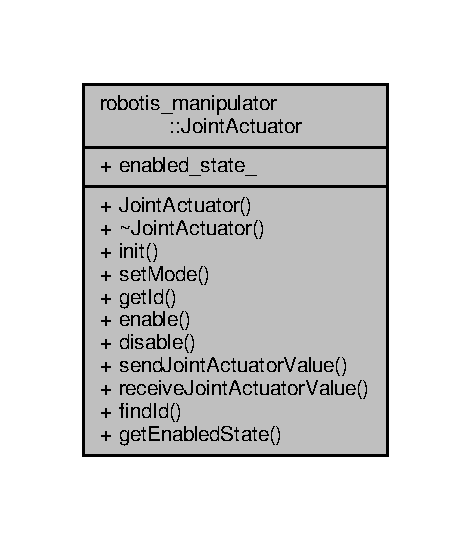
\includegraphics[width=226pt]{classrobotis__manipulator_1_1_joint_actuator__coll__graph}
\end{center}
\end{figure}
\subsection*{Public Member Functions}
\begin{DoxyCompactItemize}
\item 
\hyperlink{classrobotis__manipulator_1_1_joint_actuator_a105f09b15736f833bdb7ee3007c02a43}{Joint\+Actuator} ()
\item 
virtual \hyperlink{classrobotis__manipulator_1_1_joint_actuator_a8ecdaaabb57c7e0774f49779f756d488}{$\sim$\+Joint\+Actuator} ()
\item 
virtual void \hyperlink{classrobotis__manipulator_1_1_joint_actuator_a8573f4c73d9653d0dafc2178fca85c71}{init} (std\+::vector$<$ uint8\+\_\+t $>$ actuator\+\_\+id, const void $\ast$arg)=0
\begin{DoxyCompactList}\small\item\em init \end{DoxyCompactList}\item 
virtual void \hyperlink{classrobotis__manipulator_1_1_joint_actuator_a326759d58b0d95f4140c7615c585534d}{set\+Mode} (std\+::vector$<$ uint8\+\_\+t $>$ actuator\+\_\+id, const void $\ast$arg)=0
\begin{DoxyCompactList}\small\item\em set\+Mode \end{DoxyCompactList}\item 
virtual std\+::vector$<$ uint8\+\_\+t $>$ \hyperlink{classrobotis__manipulator_1_1_joint_actuator_a6ba533ba29c662db7c806762735e9c9c}{get\+Id} ()=0
\begin{DoxyCompactList}\small\item\em get\+Id \end{DoxyCompactList}\item 
virtual void \hyperlink{classrobotis__manipulator_1_1_joint_actuator_a08e3ca20664d47a12810b0c3cec38b5b}{enable} ()=0
\begin{DoxyCompactList}\small\item\em enable \end{DoxyCompactList}\item 
virtual void \hyperlink{classrobotis__manipulator_1_1_joint_actuator_a44f91bec9d60f61fe9158d94051602a7}{disable} ()=0
\begin{DoxyCompactList}\small\item\em disable \end{DoxyCompactList}\item 
virtual bool \hyperlink{classrobotis__manipulator_1_1_joint_actuator_abfae426680e7567920b54afd1f5c585a}{send\+Joint\+Actuator\+Value} (std\+::vector$<$ uint8\+\_\+t $>$ actuator\+\_\+id, std\+::vector$<$ \hyperlink{namespacerobotis__manipulator_a26f478d98222f9ce1bf66c7df248037b}{Actuator\+Value} $>$ value\+\_\+vector)=0
\begin{DoxyCompactList}\small\item\em send\+Joint\+Actuator\+Value \end{DoxyCompactList}\item 
virtual std\+::vector$<$ \hyperlink{namespacerobotis__manipulator_a26f478d98222f9ce1bf66c7df248037b}{Actuator\+Value} $>$ \hyperlink{classrobotis__manipulator_1_1_joint_actuator_a19c2c68427ec015516709dbe6b284688}{receive\+Joint\+Actuator\+Value} (std\+::vector$<$ uint8\+\_\+t $>$ actuator\+\_\+id)=0
\begin{DoxyCompactList}\small\item\em receive\+Joint\+Actuator\+Value \end{DoxyCompactList}\item 
bool \hyperlink{classrobotis__manipulator_1_1_joint_actuator_a1d096f6f6de5506e003ba05621ec5d33}{find\+Id} (uint8\+\_\+t actuator\+\_\+id)
\begin{DoxyCompactList}\small\item\em find\+Id \end{DoxyCompactList}\item 
bool \hyperlink{classrobotis__manipulator_1_1_joint_actuator_aff85f4ec7a489e770c4f6130cdf961ae}{get\+Enabled\+State} ()
\begin{DoxyCompactList}\small\item\em get\+Enabled\+State \end{DoxyCompactList}\end{DoxyCompactItemize}
\subsection*{Public Attributes}
\begin{DoxyCompactItemize}
\item 
bool \hyperlink{classrobotis__manipulator_1_1_joint_actuator_a62a6eaa962983ecd3948d5b9fecae79b}{enabled\+\_\+state\+\_\+}
\end{DoxyCompactItemize}


\subsection{Detailed Description}
The \hyperlink{classrobotis__manipulator_1_1_joint_actuator}{Joint\+Actuator} class. 

Definition at line 78 of file robotis\+\_\+manipulator\+\_\+manager.\+h.



\subsection{Constructor \& Destructor Documentation}
\index{robotis\+\_\+manipulator\+::\+Joint\+Actuator@{robotis\+\_\+manipulator\+::\+Joint\+Actuator}!Joint\+Actuator@{Joint\+Actuator}}
\index{Joint\+Actuator@{Joint\+Actuator}!robotis\+\_\+manipulator\+::\+Joint\+Actuator@{robotis\+\_\+manipulator\+::\+Joint\+Actuator}}
\subsubsection[{\texorpdfstring{Joint\+Actuator()}{JointActuator()}}]{\setlength{\rightskip}{0pt plus 5cm}robotis\+\_\+manipulator\+::\+Joint\+Actuator\+::\+Joint\+Actuator (
\begin{DoxyParamCaption}
{}
\end{DoxyParamCaption}
)\hspace{0.3cm}{\ttfamily [inline]}}\hypertarget{classrobotis__manipulator_1_1_joint_actuator_a105f09b15736f833bdb7ee3007c02a43}{}\label{classrobotis__manipulator_1_1_joint_actuator_a105f09b15736f833bdb7ee3007c02a43}


Definition at line 83 of file robotis\+\_\+manipulator\+\_\+manager.\+h.


\begin{DoxyCode}
83 : \hyperlink{classrobotis__manipulator_1_1_joint_actuator_a62a6eaa962983ecd3948d5b9fecae79b}{enabled\_state\_}(\textcolor{keyword}{false}) \{\}
\end{DoxyCode}
\index{robotis\+\_\+manipulator\+::\+Joint\+Actuator@{robotis\+\_\+manipulator\+::\+Joint\+Actuator}!````~Joint\+Actuator@{$\sim$\+Joint\+Actuator}}
\index{````~Joint\+Actuator@{$\sim$\+Joint\+Actuator}!robotis\+\_\+manipulator\+::\+Joint\+Actuator@{robotis\+\_\+manipulator\+::\+Joint\+Actuator}}
\subsubsection[{\texorpdfstring{$\sim$\+Joint\+Actuator()}{~JointActuator()}}]{\setlength{\rightskip}{0pt plus 5cm}virtual robotis\+\_\+manipulator\+::\+Joint\+Actuator\+::$\sim$\+Joint\+Actuator (
\begin{DoxyParamCaption}
{}
\end{DoxyParamCaption}
)\hspace{0.3cm}{\ttfamily [inline]}, {\ttfamily [virtual]}}\hypertarget{classrobotis__manipulator_1_1_joint_actuator_a8ecdaaabb57c7e0774f49779f756d488}{}\label{classrobotis__manipulator_1_1_joint_actuator_a8ecdaaabb57c7e0774f49779f756d488}


Definition at line 84 of file robotis\+\_\+manipulator\+\_\+manager.\+h.


\begin{DoxyCode}
84 \{\}
\end{DoxyCode}


\subsection{Member Function Documentation}
\index{robotis\+\_\+manipulator\+::\+Joint\+Actuator@{robotis\+\_\+manipulator\+::\+Joint\+Actuator}!disable@{disable}}
\index{disable@{disable}!robotis\+\_\+manipulator\+::\+Joint\+Actuator@{robotis\+\_\+manipulator\+::\+Joint\+Actuator}}
\subsubsection[{\texorpdfstring{disable()=0}{disable()=0}}]{\setlength{\rightskip}{0pt plus 5cm}virtual void robotis\+\_\+manipulator\+::\+Joint\+Actuator\+::disable (
\begin{DoxyParamCaption}
{}
\end{DoxyParamCaption}
)\hspace{0.3cm}{\ttfamily [pure virtual]}}\hypertarget{classrobotis__manipulator_1_1_joint_actuator_a44f91bec9d60f61fe9158d94051602a7}{}\label{classrobotis__manipulator_1_1_joint_actuator_a44f91bec9d60f61fe9158d94051602a7}


disable 

\index{robotis\+\_\+manipulator\+::\+Joint\+Actuator@{robotis\+\_\+manipulator\+::\+Joint\+Actuator}!enable@{enable}}
\index{enable@{enable}!robotis\+\_\+manipulator\+::\+Joint\+Actuator@{robotis\+\_\+manipulator\+::\+Joint\+Actuator}}
\subsubsection[{\texorpdfstring{enable()=0}{enable()=0}}]{\setlength{\rightskip}{0pt plus 5cm}virtual void robotis\+\_\+manipulator\+::\+Joint\+Actuator\+::enable (
\begin{DoxyParamCaption}
{}
\end{DoxyParamCaption}
)\hspace{0.3cm}{\ttfamily [pure virtual]}}\hypertarget{classrobotis__manipulator_1_1_joint_actuator_a08e3ca20664d47a12810b0c3cec38b5b}{}\label{classrobotis__manipulator_1_1_joint_actuator_a08e3ca20664d47a12810b0c3cec38b5b}


enable 

\index{robotis\+\_\+manipulator\+::\+Joint\+Actuator@{robotis\+\_\+manipulator\+::\+Joint\+Actuator}!find\+Id@{find\+Id}}
\index{find\+Id@{find\+Id}!robotis\+\_\+manipulator\+::\+Joint\+Actuator@{robotis\+\_\+manipulator\+::\+Joint\+Actuator}}
\subsubsection[{\texorpdfstring{find\+Id(uint8\+\_\+t actuator\+\_\+id)}{findId(uint8_t actuator_id)}}]{\setlength{\rightskip}{0pt plus 5cm}bool Joint\+Actuator\+::find\+Id (
\begin{DoxyParamCaption}
\item[{uint8\+\_\+t}]{actuator\+\_\+id}
\end{DoxyParamCaption}
)}\hypertarget{classrobotis__manipulator_1_1_joint_actuator_a1d096f6f6de5506e003ba05621ec5d33}{}\label{classrobotis__manipulator_1_1_joint_actuator_a1d096f6f6de5506e003ba05621ec5d33}


find\+Id 


\begin{DoxyParams}{Parameters}
{\em actuator\+\_\+id} & \\
\hline
\end{DoxyParams}
\begin{DoxyReturn}{Returns}

\end{DoxyReturn}


Definition at line 30 of file robotis\+\_\+manipulator\+\_\+manager.\+cpp.


\begin{DoxyCode}
31 \{
32   std::vector<uint8\_t> \textcolor{keywordtype}{id} = \hyperlink{classrobotis__manipulator_1_1_joint_actuator_a6ba533ba29c662db7c806762735e9c9c}{getId}();
33   \textcolor{keywordflow}{for}(uint32\_t index = 0; index < \textcolor{keywordtype}{id}.size(); index++)
34   \{
35     \textcolor{keywordflow}{if}(\textcolor{keywordtype}{id}.at(index) == actuator\_id)
36       \textcolor{keywordflow}{return} \textcolor{keyword}{true};
37   \}
38   \textcolor{keywordflow}{return} \textcolor{keyword}{false};
39 \}
\end{DoxyCode}


Here is the call graph for this function\+:\nopagebreak
\begin{figure}[H]
\begin{center}
\leavevmode
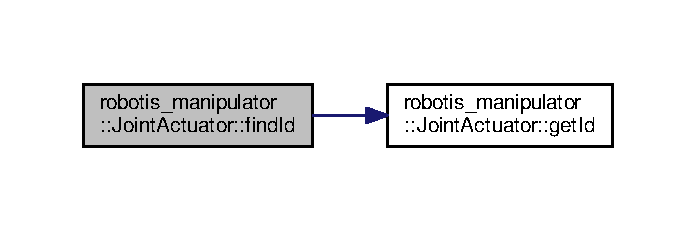
\includegraphics[width=334pt]{classrobotis__manipulator_1_1_joint_actuator_a1d096f6f6de5506e003ba05621ec5d33_cgraph}
\end{center}
\end{figure}


\index{robotis\+\_\+manipulator\+::\+Joint\+Actuator@{robotis\+\_\+manipulator\+::\+Joint\+Actuator}!get\+Enabled\+State@{get\+Enabled\+State}}
\index{get\+Enabled\+State@{get\+Enabled\+State}!robotis\+\_\+manipulator\+::\+Joint\+Actuator@{robotis\+\_\+manipulator\+::\+Joint\+Actuator}}
\subsubsection[{\texorpdfstring{get\+Enabled\+State()}{getEnabledState()}}]{\setlength{\rightskip}{0pt plus 5cm}bool Joint\+Actuator\+::get\+Enabled\+State (
\begin{DoxyParamCaption}
{}
\end{DoxyParamCaption}
)}\hypertarget{classrobotis__manipulator_1_1_joint_actuator_aff85f4ec7a489e770c4f6130cdf961ae}{}\label{classrobotis__manipulator_1_1_joint_actuator_aff85f4ec7a489e770c4f6130cdf961ae}


get\+Enabled\+State 

\begin{DoxyReturn}{Returns}

\end{DoxyReturn}


Definition at line 41 of file robotis\+\_\+manipulator\+\_\+manager.\+cpp.


\begin{DoxyCode}
42 \{
43   \textcolor{keywordflow}{return} \hyperlink{classrobotis__manipulator_1_1_joint_actuator_a62a6eaa962983ecd3948d5b9fecae79b}{enabled\_state\_};
44 \}
\end{DoxyCode}
\index{robotis\+\_\+manipulator\+::\+Joint\+Actuator@{robotis\+\_\+manipulator\+::\+Joint\+Actuator}!get\+Id@{get\+Id}}
\index{get\+Id@{get\+Id}!robotis\+\_\+manipulator\+::\+Joint\+Actuator@{robotis\+\_\+manipulator\+::\+Joint\+Actuator}}
\subsubsection[{\texorpdfstring{get\+Id()=0}{getId()=0}}]{\setlength{\rightskip}{0pt plus 5cm}virtual std\+::vector$<$uint8\+\_\+t$>$ robotis\+\_\+manipulator\+::\+Joint\+Actuator\+::get\+Id (
\begin{DoxyParamCaption}
{}
\end{DoxyParamCaption}
)\hspace{0.3cm}{\ttfamily [pure virtual]}}\hypertarget{classrobotis__manipulator_1_1_joint_actuator_a6ba533ba29c662db7c806762735e9c9c}{}\label{classrobotis__manipulator_1_1_joint_actuator_a6ba533ba29c662db7c806762735e9c9c}


get\+Id 

\begin{DoxyReturn}{Returns}

\end{DoxyReturn}


Here is the caller graph for this function\+:\nopagebreak
\begin{figure}[H]
\begin{center}
\leavevmode
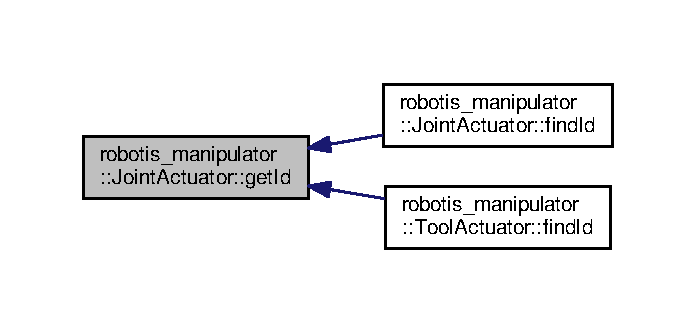
\includegraphics[width=334pt]{classrobotis__manipulator_1_1_joint_actuator_a6ba533ba29c662db7c806762735e9c9c_icgraph}
\end{center}
\end{figure}


\index{robotis\+\_\+manipulator\+::\+Joint\+Actuator@{robotis\+\_\+manipulator\+::\+Joint\+Actuator}!init@{init}}
\index{init@{init}!robotis\+\_\+manipulator\+::\+Joint\+Actuator@{robotis\+\_\+manipulator\+::\+Joint\+Actuator}}
\subsubsection[{\texorpdfstring{init(std\+::vector$<$ uint8\+\_\+t $>$ actuator\+\_\+id, const void $\ast$arg)=0}{init(std::vector< uint8_t > actuator_id, const void *arg)=0}}]{\setlength{\rightskip}{0pt plus 5cm}virtual void robotis\+\_\+manipulator\+::\+Joint\+Actuator\+::init (
\begin{DoxyParamCaption}
\item[{std\+::vector$<$ uint8\+\_\+t $>$}]{actuator\+\_\+id, }
\item[{const void $\ast$}]{arg}
\end{DoxyParamCaption}
)\hspace{0.3cm}{\ttfamily [pure virtual]}}\hypertarget{classrobotis__manipulator_1_1_joint_actuator_a8573f4c73d9653d0dafc2178fca85c71}{}\label{classrobotis__manipulator_1_1_joint_actuator_a8573f4c73d9653d0dafc2178fca85c71}


init 


\begin{DoxyParams}{Parameters}
{\em actuator\+\_\+id} & \\
\hline
{\em arg} & \\
\hline
\end{DoxyParams}
\index{robotis\+\_\+manipulator\+::\+Joint\+Actuator@{robotis\+\_\+manipulator\+::\+Joint\+Actuator}!receive\+Joint\+Actuator\+Value@{receive\+Joint\+Actuator\+Value}}
\index{receive\+Joint\+Actuator\+Value@{receive\+Joint\+Actuator\+Value}!robotis\+\_\+manipulator\+::\+Joint\+Actuator@{robotis\+\_\+manipulator\+::\+Joint\+Actuator}}
\subsubsection[{\texorpdfstring{receive\+Joint\+Actuator\+Value(std\+::vector$<$ uint8\+\_\+t $>$ actuator\+\_\+id)=0}{receiveJointActuatorValue(std::vector< uint8_t > actuator_id)=0}}]{\setlength{\rightskip}{0pt plus 5cm}virtual std\+::vector$<${\bf Actuator\+Value}$>$ robotis\+\_\+manipulator\+::\+Joint\+Actuator\+::receive\+Joint\+Actuator\+Value (
\begin{DoxyParamCaption}
\item[{std\+::vector$<$ uint8\+\_\+t $>$}]{actuator\+\_\+id}
\end{DoxyParamCaption}
)\hspace{0.3cm}{\ttfamily [pure virtual]}}\hypertarget{classrobotis__manipulator_1_1_joint_actuator_a19c2c68427ec015516709dbe6b284688}{}\label{classrobotis__manipulator_1_1_joint_actuator_a19c2c68427ec015516709dbe6b284688}


receive\+Joint\+Actuator\+Value 


\begin{DoxyParams}{Parameters}
{\em actuator\+\_\+id} & \\
\hline
\end{DoxyParams}
\begin{DoxyReturn}{Returns}

\end{DoxyReturn}
\index{robotis\+\_\+manipulator\+::\+Joint\+Actuator@{robotis\+\_\+manipulator\+::\+Joint\+Actuator}!send\+Joint\+Actuator\+Value@{send\+Joint\+Actuator\+Value}}
\index{send\+Joint\+Actuator\+Value@{send\+Joint\+Actuator\+Value}!robotis\+\_\+manipulator\+::\+Joint\+Actuator@{robotis\+\_\+manipulator\+::\+Joint\+Actuator}}
\subsubsection[{\texorpdfstring{send\+Joint\+Actuator\+Value(std\+::vector$<$ uint8\+\_\+t $>$ actuator\+\_\+id, std\+::vector$<$ Actuator\+Value $>$ value\+\_\+vector)=0}{sendJointActuatorValue(std::vector< uint8_t > actuator_id, std::vector< ActuatorValue > value_vector)=0}}]{\setlength{\rightskip}{0pt plus 5cm}virtual bool robotis\+\_\+manipulator\+::\+Joint\+Actuator\+::send\+Joint\+Actuator\+Value (
\begin{DoxyParamCaption}
\item[{std\+::vector$<$ uint8\+\_\+t $>$}]{actuator\+\_\+id, }
\item[{std\+::vector$<$ {\bf Actuator\+Value} $>$}]{value\+\_\+vector}
\end{DoxyParamCaption}
)\hspace{0.3cm}{\ttfamily [pure virtual]}}\hypertarget{classrobotis__manipulator_1_1_joint_actuator_abfae426680e7567920b54afd1f5c585a}{}\label{classrobotis__manipulator_1_1_joint_actuator_abfae426680e7567920b54afd1f5c585a}


send\+Joint\+Actuator\+Value 


\begin{DoxyParams}{Parameters}
{\em actuator\+\_\+id} & \\
\hline
{\em value\+\_\+vector} & \\
\hline
\end{DoxyParams}
\begin{DoxyReturn}{Returns}

\end{DoxyReturn}
\index{robotis\+\_\+manipulator\+::\+Joint\+Actuator@{robotis\+\_\+manipulator\+::\+Joint\+Actuator}!set\+Mode@{set\+Mode}}
\index{set\+Mode@{set\+Mode}!robotis\+\_\+manipulator\+::\+Joint\+Actuator@{robotis\+\_\+manipulator\+::\+Joint\+Actuator}}
\subsubsection[{\texorpdfstring{set\+Mode(std\+::vector$<$ uint8\+\_\+t $>$ actuator\+\_\+id, const void $\ast$arg)=0}{setMode(std::vector< uint8_t > actuator_id, const void *arg)=0}}]{\setlength{\rightskip}{0pt plus 5cm}virtual void robotis\+\_\+manipulator\+::\+Joint\+Actuator\+::set\+Mode (
\begin{DoxyParamCaption}
\item[{std\+::vector$<$ uint8\+\_\+t $>$}]{actuator\+\_\+id, }
\item[{const void $\ast$}]{arg}
\end{DoxyParamCaption}
)\hspace{0.3cm}{\ttfamily [pure virtual]}}\hypertarget{classrobotis__manipulator_1_1_joint_actuator_a326759d58b0d95f4140c7615c585534d}{}\label{classrobotis__manipulator_1_1_joint_actuator_a326759d58b0d95f4140c7615c585534d}


set\+Mode 


\begin{DoxyParams}{Parameters}
{\em actuator\+\_\+id} & \\
\hline
{\em arg} & \\
\hline
\end{DoxyParams}


\subsection{Member Data Documentation}
\index{robotis\+\_\+manipulator\+::\+Joint\+Actuator@{robotis\+\_\+manipulator\+::\+Joint\+Actuator}!enabled\+\_\+state\+\_\+@{enabled\+\_\+state\+\_\+}}
\index{enabled\+\_\+state\+\_\+@{enabled\+\_\+state\+\_\+}!robotis\+\_\+manipulator\+::\+Joint\+Actuator@{robotis\+\_\+manipulator\+::\+Joint\+Actuator}}
\subsubsection[{\texorpdfstring{enabled\+\_\+state\+\_\+}{enabled_state_}}]{\setlength{\rightskip}{0pt plus 5cm}bool robotis\+\_\+manipulator\+::\+Joint\+Actuator\+::enabled\+\_\+state\+\_\+}\hypertarget{classrobotis__manipulator_1_1_joint_actuator_a62a6eaa962983ecd3948d5b9fecae79b}{}\label{classrobotis__manipulator_1_1_joint_actuator_a62a6eaa962983ecd3948d5b9fecae79b}


Definition at line 81 of file robotis\+\_\+manipulator\+\_\+manager.\+h.



The documentation for this class was generated from the following files\+:\begin{DoxyCompactItemize}
\item 
include/robotis\+\_\+manipulator/\hyperlink{robotis__manipulator__manager_8h}{robotis\+\_\+manipulator\+\_\+manager.\+h}\item 
src/robotis\+\_\+manipulator/\hyperlink{robotis__manipulator__manager_8cpp}{robotis\+\_\+manipulator\+\_\+manager.\+cpp}\end{DoxyCompactItemize}

\hypertarget{structrobotis__manipulator_1_1_joint_constant}{}\section{robotis\+\_\+manipulator\+:\+:Joint\+Constant Struct Reference}
\label{structrobotis__manipulator_1_1_joint_constant}\index{robotis\+\_\+manipulator\+::\+Joint\+Constant@{robotis\+\_\+manipulator\+::\+Joint\+Constant}}


{\ttfamily \#include $<$robotis\+\_\+manipulator\+\_\+common.\+h$>$}



Collaboration diagram for robotis\+\_\+manipulator\+:\+:Joint\+Constant\+:\nopagebreak
\begin{figure}[H]
\begin{center}
\leavevmode
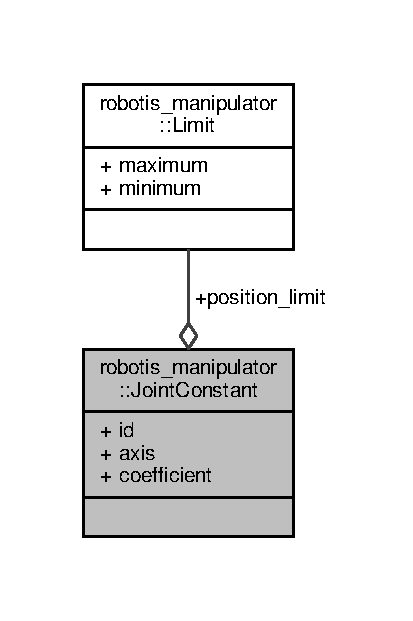
\includegraphics[width=198pt]{structrobotis__manipulator_1_1_joint_constant__coll__graph}
\end{center}
\end{figure}
\subsection*{Public Attributes}
\begin{DoxyCompactItemize}
\item 
int8\+\_\+t \hyperlink{structrobotis__manipulator_1_1_joint_constant_ac4e09e4e2886029c58d6f727e9b1e274}{id}
\item 
Eigen\+::\+Vector3d \hyperlink{structrobotis__manipulator_1_1_joint_constant_aa3bf091d44be75bd46e5052fd32fccc6}{axis}
\item 
double \hyperlink{structrobotis__manipulator_1_1_joint_constant_acd88ff436867374790745f4661b12821}{coefficient}
\item 
\hyperlink{structrobotis__manipulator_1_1_limit}{Limit} \hyperlink{structrobotis__manipulator_1_1_joint_constant_a15c9d0a10c81d861a1d4762b0f9a790d}{position\+\_\+limit}
\end{DoxyCompactItemize}


\subsection{Detailed Description}


Definition at line 145 of file robotis\+\_\+manipulator\+\_\+common.\+h.



\subsection{Member Data Documentation}
\index{robotis\+\_\+manipulator\+::\+Joint\+Constant@{robotis\+\_\+manipulator\+::\+Joint\+Constant}!axis@{axis}}
\index{axis@{axis}!robotis\+\_\+manipulator\+::\+Joint\+Constant@{robotis\+\_\+manipulator\+::\+Joint\+Constant}}
\subsubsection[{\texorpdfstring{axis}{axis}}]{\setlength{\rightskip}{0pt plus 5cm}Eigen\+::\+Vector3d robotis\+\_\+manipulator\+::\+Joint\+Constant\+::axis}\hypertarget{structrobotis__manipulator_1_1_joint_constant_aa3bf091d44be75bd46e5052fd32fccc6}{}\label{structrobotis__manipulator_1_1_joint_constant_aa3bf091d44be75bd46e5052fd32fccc6}


Definition at line 148 of file robotis\+\_\+manipulator\+\_\+common.\+h.

\index{robotis\+\_\+manipulator\+::\+Joint\+Constant@{robotis\+\_\+manipulator\+::\+Joint\+Constant}!coefficient@{coefficient}}
\index{coefficient@{coefficient}!robotis\+\_\+manipulator\+::\+Joint\+Constant@{robotis\+\_\+manipulator\+::\+Joint\+Constant}}
\subsubsection[{\texorpdfstring{coefficient}{coefficient}}]{\setlength{\rightskip}{0pt plus 5cm}double robotis\+\_\+manipulator\+::\+Joint\+Constant\+::coefficient}\hypertarget{structrobotis__manipulator_1_1_joint_constant_acd88ff436867374790745f4661b12821}{}\label{structrobotis__manipulator_1_1_joint_constant_acd88ff436867374790745f4661b12821}


Definition at line 149 of file robotis\+\_\+manipulator\+\_\+common.\+h.

\index{robotis\+\_\+manipulator\+::\+Joint\+Constant@{robotis\+\_\+manipulator\+::\+Joint\+Constant}!id@{id}}
\index{id@{id}!robotis\+\_\+manipulator\+::\+Joint\+Constant@{robotis\+\_\+manipulator\+::\+Joint\+Constant}}
\subsubsection[{\texorpdfstring{id}{id}}]{\setlength{\rightskip}{0pt plus 5cm}int8\+\_\+t robotis\+\_\+manipulator\+::\+Joint\+Constant\+::id}\hypertarget{structrobotis__manipulator_1_1_joint_constant_ac4e09e4e2886029c58d6f727e9b1e274}{}\label{structrobotis__manipulator_1_1_joint_constant_ac4e09e4e2886029c58d6f727e9b1e274}


Definition at line 147 of file robotis\+\_\+manipulator\+\_\+common.\+h.

\index{robotis\+\_\+manipulator\+::\+Joint\+Constant@{robotis\+\_\+manipulator\+::\+Joint\+Constant}!position\+\_\+limit@{position\+\_\+limit}}
\index{position\+\_\+limit@{position\+\_\+limit}!robotis\+\_\+manipulator\+::\+Joint\+Constant@{robotis\+\_\+manipulator\+::\+Joint\+Constant}}
\subsubsection[{\texorpdfstring{position\+\_\+limit}{position_limit}}]{\setlength{\rightskip}{0pt plus 5cm}{\bf Limit} robotis\+\_\+manipulator\+::\+Joint\+Constant\+::position\+\_\+limit}\hypertarget{structrobotis__manipulator_1_1_joint_constant_a15c9d0a10c81d861a1d4762b0f9a790d}{}\label{structrobotis__manipulator_1_1_joint_constant_a15c9d0a10c81d861a1d4762b0f9a790d}


Definition at line 150 of file robotis\+\_\+manipulator\+\_\+common.\+h.



The documentation for this struct was generated from the following file\+:\begin{DoxyCompactItemize}
\item 
include/robotis\+\_\+manipulator/\hyperlink{robotis__manipulator__common_8h}{robotis\+\_\+manipulator\+\_\+common.\+h}\end{DoxyCompactItemize}

\hypertarget{classrobotis__manipulator_1_1_joint_trajectory}{}\section{robotis\+\_\+manipulator\+:\+:Joint\+Trajectory Class Reference}
\label{classrobotis__manipulator_1_1_joint_trajectory}\index{robotis\+\_\+manipulator\+::\+Joint\+Trajectory@{robotis\+\_\+manipulator\+::\+Joint\+Trajectory}}


The \hyperlink{classrobotis__manipulator_1_1_joint_trajectory}{Joint\+Trajectory} class.  




{\ttfamily \#include $<$robotis\+\_\+manipulator\+\_\+trajectory\+\_\+generator.\+h$>$}



Collaboration diagram for robotis\+\_\+manipulator\+:\+:Joint\+Trajectory\+:\nopagebreak
\begin{figure}[H]
\begin{center}
\leavevmode
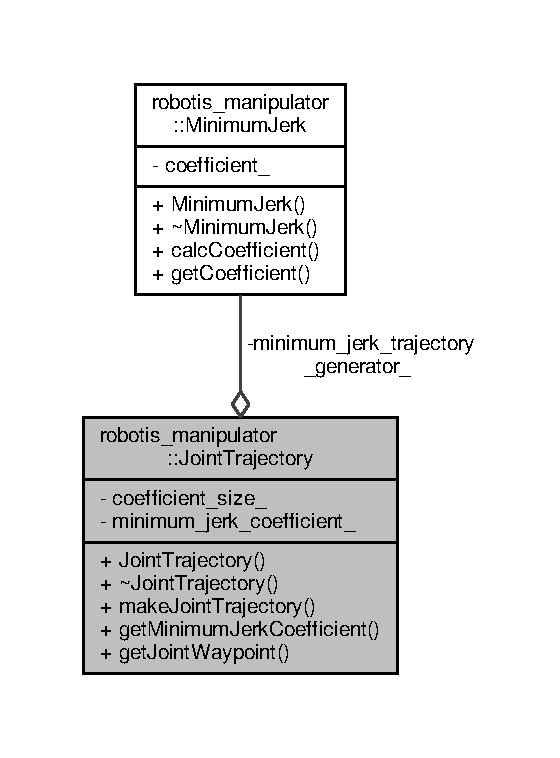
\includegraphics[width=269pt]{classrobotis__manipulator_1_1_joint_trajectory__coll__graph}
\end{center}
\end{figure}
\subsection*{Public Member Functions}
\begin{DoxyCompactItemize}
\item 
\hyperlink{classrobotis__manipulator_1_1_joint_trajectory_abeaf864dbc1fa619ca8870c03f36f8b5}{Joint\+Trajectory} ()
\item 
virtual \hyperlink{classrobotis__manipulator_1_1_joint_trajectory_a971255bd9c193d9c333f1c095692f7e3}{$\sim$\+Joint\+Trajectory} ()
\item 
void \hyperlink{classrobotis__manipulator_1_1_joint_trajectory_a27165ae6c8bc5ffd3d431ac03c77cddb}{make\+Joint\+Trajectory} (double move\+\_\+time, \hyperlink{namespacerobotis__manipulator_a4456fd8b14e1f6b7733a77837dfe9339}{Joint\+Waypoint} start, \hyperlink{namespacerobotis__manipulator_a4456fd8b14e1f6b7733a77837dfe9339}{Joint\+Waypoint} goal)
\begin{DoxyCompactList}\small\item\em make\+Joint\+Trajectory \end{DoxyCompactList}\item 
Eigen\+::\+Matrix\+Xd \hyperlink{classrobotis__manipulator_1_1_joint_trajectory_a2a471ffc50baf5d83bd857ea57ed3ccd}{get\+Minimum\+Jerk\+Coefficient} ()
\begin{DoxyCompactList}\small\item\em get\+Minimum\+Jerk\+Coefficient \end{DoxyCompactList}\item 
\hyperlink{namespacerobotis__manipulator_a4456fd8b14e1f6b7733a77837dfe9339}{Joint\+Waypoint} \hyperlink{classrobotis__manipulator_1_1_joint_trajectory_aef1a0eaac83af6599f2bef674d299f4c}{get\+Joint\+Waypoint} (double tick)
\begin{DoxyCompactList}\small\item\em get\+Joint\+Waypoint \end{DoxyCompactList}\end{DoxyCompactItemize}
\subsection*{Private Attributes}
\begin{DoxyCompactItemize}
\item 
uint8\+\_\+t \hyperlink{classrobotis__manipulator_1_1_joint_trajectory_abfc3d7ff3a5789f818ce2a483118458a}{coefficient\+\_\+size\+\_\+}
\item 
\hyperlink{classrobotis__manipulator_1_1_minimum_jerk}{Minimum\+Jerk} \hyperlink{classrobotis__manipulator_1_1_joint_trajectory_a7138717ca5cd53ca07e3ff9c68494170}{minimum\+\_\+jerk\+\_\+trajectory\+\_\+generator\+\_\+}
\item 
Eigen\+::\+Matrix\+Xd \hyperlink{classrobotis__manipulator_1_1_joint_trajectory_a74b431132c75c6840b70ea62f65d3c48}{minimum\+\_\+jerk\+\_\+coefficient\+\_\+}
\end{DoxyCompactItemize}


\subsection{Detailed Description}
The \hyperlink{classrobotis__manipulator_1_1_joint_trajectory}{Joint\+Trajectory} class. 

Definition at line 79 of file robotis\+\_\+manipulator\+\_\+trajectory\+\_\+generator.\+h.



\subsection{Constructor \& Destructor Documentation}
\index{robotis\+\_\+manipulator\+::\+Joint\+Trajectory@{robotis\+\_\+manipulator\+::\+Joint\+Trajectory}!Joint\+Trajectory@{Joint\+Trajectory}}
\index{Joint\+Trajectory@{Joint\+Trajectory}!robotis\+\_\+manipulator\+::\+Joint\+Trajectory@{robotis\+\_\+manipulator\+::\+Joint\+Trajectory}}
\subsubsection[{\texorpdfstring{Joint\+Trajectory()}{JointTrajectory()}}]{\setlength{\rightskip}{0pt plus 5cm}Joint\+Trajectory\+::\+Joint\+Trajectory (
\begin{DoxyParamCaption}
{}
\end{DoxyParamCaption}
)}\hypertarget{classrobotis__manipulator_1_1_joint_trajectory_abeaf864dbc1fa619ca8870c03f36f8b5}{}\label{classrobotis__manipulator_1_1_joint_trajectory_abeaf864dbc1fa619ca8870c03f36f8b5}


Definition at line 72 of file robotis\+\_\+manipulator\+\_\+trajectory\+\_\+generator.\+cpp.


\begin{DoxyCode}
73 \{\}
\end{DoxyCode}
\index{robotis\+\_\+manipulator\+::\+Joint\+Trajectory@{robotis\+\_\+manipulator\+::\+Joint\+Trajectory}!````~Joint\+Trajectory@{$\sim$\+Joint\+Trajectory}}
\index{````~Joint\+Trajectory@{$\sim$\+Joint\+Trajectory}!robotis\+\_\+manipulator\+::\+Joint\+Trajectory@{robotis\+\_\+manipulator\+::\+Joint\+Trajectory}}
\subsubsection[{\texorpdfstring{$\sim$\+Joint\+Trajectory()}{~JointTrajectory()}}]{\setlength{\rightskip}{0pt plus 5cm}Joint\+Trajectory\+::$\sim$\+Joint\+Trajectory (
\begin{DoxyParamCaption}
{}
\end{DoxyParamCaption}
)\hspace{0.3cm}{\ttfamily [virtual]}}\hypertarget{classrobotis__manipulator_1_1_joint_trajectory_a971255bd9c193d9c333f1c095692f7e3}{}\label{classrobotis__manipulator_1_1_joint_trajectory_a971255bd9c193d9c333f1c095692f7e3}


Definition at line 75 of file robotis\+\_\+manipulator\+\_\+trajectory\+\_\+generator.\+cpp.


\begin{DoxyCode}
75 \{\}
\end{DoxyCode}


\subsection{Member Function Documentation}
\index{robotis\+\_\+manipulator\+::\+Joint\+Trajectory@{robotis\+\_\+manipulator\+::\+Joint\+Trajectory}!get\+Joint\+Waypoint@{get\+Joint\+Waypoint}}
\index{get\+Joint\+Waypoint@{get\+Joint\+Waypoint}!robotis\+\_\+manipulator\+::\+Joint\+Trajectory@{robotis\+\_\+manipulator\+::\+Joint\+Trajectory}}
\subsubsection[{\texorpdfstring{get\+Joint\+Waypoint(double tick)}{getJointWaypoint(double tick)}}]{\setlength{\rightskip}{0pt plus 5cm}{\bf Joint\+Waypoint} Joint\+Trajectory\+::get\+Joint\+Waypoint (
\begin{DoxyParamCaption}
\item[{double}]{tick}
\end{DoxyParamCaption}
)}\hypertarget{classrobotis__manipulator_1_1_joint_trajectory_aef1a0eaac83af6599f2bef674d299f4c}{}\label{classrobotis__manipulator_1_1_joint_trajectory_aef1a0eaac83af6599f2bef674d299f4c}


get\+Joint\+Waypoint 


\begin{DoxyParams}{Parameters}
{\em tick} & \\
\hline
\end{DoxyParams}
\begin{DoxyReturn}{Returns}

\end{DoxyReturn}


Definition at line 92 of file robotis\+\_\+manipulator\+\_\+trajectory\+\_\+generator.\+cpp.


\begin{DoxyCode}
93 \{
94   \hyperlink{namespacerobotis__manipulator_a4456fd8b14e1f6b7733a77837dfe9339}{JointWaypoint} joint\_way\_point;
95   \textcolor{keywordflow}{for} (uint8\_t index = 0; index < \hyperlink{classrobotis__manipulator_1_1_joint_trajectory_abfc3d7ff3a5789f818ce2a483118458a}{coefficient\_size\_}; index++)
96   \{
97     \hyperlink{structrobotis__manipulator_1_1_point}{JointValue} single\_joint\_way\_point;
98 
99     single\_joint\_way\_point.\hyperlink{structrobotis__manipulator_1_1_point_a0f122386b502d9b316bdead542ed2145}{position} = \hyperlink{classrobotis__manipulator_1_1_joint_trajectory_a74b431132c75c6840b70ea62f65d3c48}{minimum\_jerk\_coefficient\_}(0, index) 
      +
100              \hyperlink{classrobotis__manipulator_1_1_joint_trajectory_a74b431132c75c6840b70ea62f65d3c48}{minimum\_jerk\_coefficient\_}(1, index) * pow(tick, 1) +
101              \hyperlink{classrobotis__manipulator_1_1_joint_trajectory_a74b431132c75c6840b70ea62f65d3c48}{minimum\_jerk\_coefficient\_}(2, index) * pow(tick, 2) +
102              \hyperlink{classrobotis__manipulator_1_1_joint_trajectory_a74b431132c75c6840b70ea62f65d3c48}{minimum\_jerk\_coefficient\_}(3, index) * pow(tick, 3) +
103              \hyperlink{classrobotis__manipulator_1_1_joint_trajectory_a74b431132c75c6840b70ea62f65d3c48}{minimum\_jerk\_coefficient\_}(4, index) * pow(tick, 4) +
104              \hyperlink{classrobotis__manipulator_1_1_joint_trajectory_a74b431132c75c6840b70ea62f65d3c48}{minimum\_jerk\_coefficient\_}(5, index) * pow(tick, 5);
105 
106     single\_joint\_way\_point.\hyperlink{structrobotis__manipulator_1_1_point_a4eaec95fac0c755eb0aa704b36ebe97b}{velocity} = \hyperlink{classrobotis__manipulator_1_1_joint_trajectory_a74b431132c75c6840b70ea62f65d3c48}{minimum\_jerk\_coefficient\_}(1, index) 
      +
107              2 * \hyperlink{classrobotis__manipulator_1_1_joint_trajectory_a74b431132c75c6840b70ea62f65d3c48}{minimum\_jerk\_coefficient\_}(2, index) * pow(tick, 1) +
108              3 * \hyperlink{classrobotis__manipulator_1_1_joint_trajectory_a74b431132c75c6840b70ea62f65d3c48}{minimum\_jerk\_coefficient\_}(3, index) * pow(tick, 2) +
109              4 * \hyperlink{classrobotis__manipulator_1_1_joint_trajectory_a74b431132c75c6840b70ea62f65d3c48}{minimum\_jerk\_coefficient\_}(4, index) * pow(tick, 3) +
110              5 * \hyperlink{classrobotis__manipulator_1_1_joint_trajectory_a74b431132c75c6840b70ea62f65d3c48}{minimum\_jerk\_coefficient\_}(5, index) * pow(tick, 4);
111 
112     single\_joint\_way\_point.\hyperlink{structrobotis__manipulator_1_1_point_adb49f1fbcc0eaa7f530c54fdf0ede836}{acceleration} = 2 * 
      \hyperlink{classrobotis__manipulator_1_1_joint_trajectory_a74b431132c75c6840b70ea62f65d3c48}{minimum\_jerk\_coefficient\_}(2, index) +
113              6 * \hyperlink{classrobotis__manipulator_1_1_joint_trajectory_a74b431132c75c6840b70ea62f65d3c48}{minimum\_jerk\_coefficient\_}(3, index) * pow(tick, 1) +
114              12 * \hyperlink{classrobotis__manipulator_1_1_joint_trajectory_a74b431132c75c6840b70ea62f65d3c48}{minimum\_jerk\_coefficient\_}(4, index) * pow(tick, 2) +
115              20 * \hyperlink{classrobotis__manipulator_1_1_joint_trajectory_a74b431132c75c6840b70ea62f65d3c48}{minimum\_jerk\_coefficient\_}(5, index) * pow(tick, 3);
116 
117     single\_joint\_way\_point.\hyperlink{structrobotis__manipulator_1_1_point_add1a7019fc87cc2ac9bdf033372a9bb6}{effort} = 0.0;
118 
119     joint\_way\_point.push\_back(single\_joint\_way\_point);
120   \}
121 
122   \textcolor{keywordflow}{return} joint\_way\_point;
123 \}
\end{DoxyCode}


Here is the caller graph for this function\+:\nopagebreak
\begin{figure}[H]
\begin{center}
\leavevmode
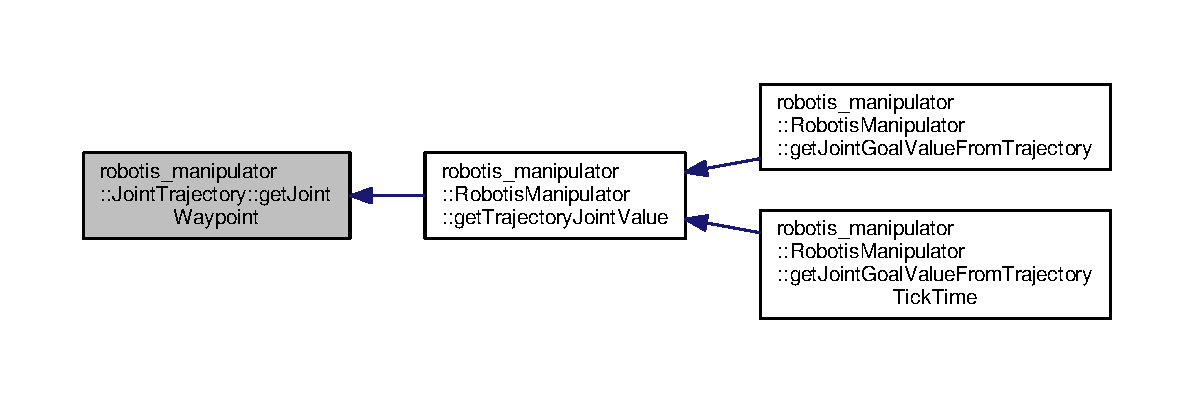
\includegraphics[width=350pt]{classrobotis__manipulator_1_1_joint_trajectory_aef1a0eaac83af6599f2bef674d299f4c_icgraph}
\end{center}
\end{figure}


\index{robotis\+\_\+manipulator\+::\+Joint\+Trajectory@{robotis\+\_\+manipulator\+::\+Joint\+Trajectory}!get\+Minimum\+Jerk\+Coefficient@{get\+Minimum\+Jerk\+Coefficient}}
\index{get\+Minimum\+Jerk\+Coefficient@{get\+Minimum\+Jerk\+Coefficient}!robotis\+\_\+manipulator\+::\+Joint\+Trajectory@{robotis\+\_\+manipulator\+::\+Joint\+Trajectory}}
\subsubsection[{\texorpdfstring{get\+Minimum\+Jerk\+Coefficient()}{getMinimumJerkCoefficient()}}]{\setlength{\rightskip}{0pt plus 5cm}Eigen\+::\+Matrix\+Xd Joint\+Trajectory\+::get\+Minimum\+Jerk\+Coefficient (
\begin{DoxyParamCaption}
{}
\end{DoxyParamCaption}
)}\hypertarget{classrobotis__manipulator_1_1_joint_trajectory_a2a471ffc50baf5d83bd857ea57ed3ccd}{}\label{classrobotis__manipulator_1_1_joint_trajectory_a2a471ffc50baf5d83bd857ea57ed3ccd}


get\+Minimum\+Jerk\+Coefficient 

\begin{DoxyReturn}{Returns}

\end{DoxyReturn}


Definition at line 125 of file robotis\+\_\+manipulator\+\_\+trajectory\+\_\+generator.\+cpp.


\begin{DoxyCode}
126 \{
127   \textcolor{keywordflow}{return} \hyperlink{classrobotis__manipulator_1_1_joint_trajectory_a74b431132c75c6840b70ea62f65d3c48}{minimum\_jerk\_coefficient\_};
128 \}
\end{DoxyCode}
\index{robotis\+\_\+manipulator\+::\+Joint\+Trajectory@{robotis\+\_\+manipulator\+::\+Joint\+Trajectory}!make\+Joint\+Trajectory@{make\+Joint\+Trajectory}}
\index{make\+Joint\+Trajectory@{make\+Joint\+Trajectory}!robotis\+\_\+manipulator\+::\+Joint\+Trajectory@{robotis\+\_\+manipulator\+::\+Joint\+Trajectory}}
\subsubsection[{\texorpdfstring{make\+Joint\+Trajectory(double move\+\_\+time, Joint\+Waypoint start, Joint\+Waypoint goal)}{makeJointTrajectory(double move_time, JointWaypoint start, JointWaypoint goal)}}]{\setlength{\rightskip}{0pt plus 5cm}void Joint\+Trajectory\+::make\+Joint\+Trajectory (
\begin{DoxyParamCaption}
\item[{double}]{move\+\_\+time, }
\item[{{\bf Joint\+Waypoint}}]{start, }
\item[{{\bf Joint\+Waypoint}}]{goal}
\end{DoxyParamCaption}
)}\hypertarget{classrobotis__manipulator_1_1_joint_trajectory_a27165ae6c8bc5ffd3d431ac03c77cddb}{}\label{classrobotis__manipulator_1_1_joint_trajectory_a27165ae6c8bc5ffd3d431ac03c77cddb}


make\+Joint\+Trajectory 


\begin{DoxyParams}{Parameters}
{\em move\+\_\+time} & \\
\hline
{\em start} & \\
\hline
{\em goal} & \\
\hline
\end{DoxyParams}


Definition at line 77 of file robotis\+\_\+manipulator\+\_\+trajectory\+\_\+generator.\+cpp.


\begin{DoxyCode}
79 \{
80   \hyperlink{classrobotis__manipulator_1_1_joint_trajectory_abfc3d7ff3a5789f818ce2a483118458a}{coefficient\_size\_} = start.size();
81   \hyperlink{classrobotis__manipulator_1_1_joint_trajectory_a74b431132c75c6840b70ea62f65d3c48}{minimum\_jerk\_coefficient\_}.resize(6,\hyperlink{classrobotis__manipulator_1_1_joint_trajectory_abfc3d7ff3a5789f818ce2a483118458a}{coefficient\_size\_});
82   \textcolor{keywordflow}{for} (uint8\_t index = 0; index < \hyperlink{classrobotis__manipulator_1_1_joint_trajectory_abfc3d7ff3a5789f818ce2a483118458a}{coefficient\_size\_}; index++)
83   \{
84     \hyperlink{classrobotis__manipulator_1_1_joint_trajectory_a7138717ca5cd53ca07e3ff9c68494170}{minimum\_jerk\_trajectory\_generator\_}.
      \hyperlink{classrobotis__manipulator_1_1_minimum_jerk_afd29204e588525a2688a74d2a9656354}{calcCoefficient}(start.at(index),
85                                     goal.at(index),
86                                     move\_time);
87 
88     \hyperlink{classrobotis__manipulator_1_1_joint_trajectory_a74b431132c75c6840b70ea62f65d3c48}{minimum\_jerk\_coefficient\_}.col(index) = 
      \hyperlink{classrobotis__manipulator_1_1_joint_trajectory_a7138717ca5cd53ca07e3ff9c68494170}{minimum\_jerk\_trajectory\_generator\_}.
      \hyperlink{classrobotis__manipulator_1_1_minimum_jerk_a1610599c85567422e492e0893e02cc34}{getCoefficient}();
89   \}
90 \}
\end{DoxyCode}


\subsection{Member Data Documentation}
\index{robotis\+\_\+manipulator\+::\+Joint\+Trajectory@{robotis\+\_\+manipulator\+::\+Joint\+Trajectory}!coefficient\+\_\+size\+\_\+@{coefficient\+\_\+size\+\_\+}}
\index{coefficient\+\_\+size\+\_\+@{coefficient\+\_\+size\+\_\+}!robotis\+\_\+manipulator\+::\+Joint\+Trajectory@{robotis\+\_\+manipulator\+::\+Joint\+Trajectory}}
\subsubsection[{\texorpdfstring{coefficient\+\_\+size\+\_\+}{coefficient_size_}}]{\setlength{\rightskip}{0pt plus 5cm}uint8\+\_\+t robotis\+\_\+manipulator\+::\+Joint\+Trajectory\+::coefficient\+\_\+size\+\_\+\hspace{0.3cm}{\ttfamily [private]}}\hypertarget{classrobotis__manipulator_1_1_joint_trajectory_abfc3d7ff3a5789f818ce2a483118458a}{}\label{classrobotis__manipulator_1_1_joint_trajectory_abfc3d7ff3a5789f818ce2a483118458a}


Definition at line 82 of file robotis\+\_\+manipulator\+\_\+trajectory\+\_\+generator.\+h.

\index{robotis\+\_\+manipulator\+::\+Joint\+Trajectory@{robotis\+\_\+manipulator\+::\+Joint\+Trajectory}!minimum\+\_\+jerk\+\_\+coefficient\+\_\+@{minimum\+\_\+jerk\+\_\+coefficient\+\_\+}}
\index{minimum\+\_\+jerk\+\_\+coefficient\+\_\+@{minimum\+\_\+jerk\+\_\+coefficient\+\_\+}!robotis\+\_\+manipulator\+::\+Joint\+Trajectory@{robotis\+\_\+manipulator\+::\+Joint\+Trajectory}}
\subsubsection[{\texorpdfstring{minimum\+\_\+jerk\+\_\+coefficient\+\_\+}{minimum_jerk_coefficient_}}]{\setlength{\rightskip}{0pt plus 5cm}Eigen\+::\+Matrix\+Xd robotis\+\_\+manipulator\+::\+Joint\+Trajectory\+::minimum\+\_\+jerk\+\_\+coefficient\+\_\+\hspace{0.3cm}{\ttfamily [private]}}\hypertarget{classrobotis__manipulator_1_1_joint_trajectory_a74b431132c75c6840b70ea62f65d3c48}{}\label{classrobotis__manipulator_1_1_joint_trajectory_a74b431132c75c6840b70ea62f65d3c48}


Definition at line 84 of file robotis\+\_\+manipulator\+\_\+trajectory\+\_\+generator.\+h.

\index{robotis\+\_\+manipulator\+::\+Joint\+Trajectory@{robotis\+\_\+manipulator\+::\+Joint\+Trajectory}!minimum\+\_\+jerk\+\_\+trajectory\+\_\+generator\+\_\+@{minimum\+\_\+jerk\+\_\+trajectory\+\_\+generator\+\_\+}}
\index{minimum\+\_\+jerk\+\_\+trajectory\+\_\+generator\+\_\+@{minimum\+\_\+jerk\+\_\+trajectory\+\_\+generator\+\_\+}!robotis\+\_\+manipulator\+::\+Joint\+Trajectory@{robotis\+\_\+manipulator\+::\+Joint\+Trajectory}}
\subsubsection[{\texorpdfstring{minimum\+\_\+jerk\+\_\+trajectory\+\_\+generator\+\_\+}{minimum_jerk_trajectory_generator_}}]{\setlength{\rightskip}{0pt plus 5cm}{\bf Minimum\+Jerk} robotis\+\_\+manipulator\+::\+Joint\+Trajectory\+::minimum\+\_\+jerk\+\_\+trajectory\+\_\+generator\+\_\+\hspace{0.3cm}{\ttfamily [private]}}\hypertarget{classrobotis__manipulator_1_1_joint_trajectory_a7138717ca5cd53ca07e3ff9c68494170}{}\label{classrobotis__manipulator_1_1_joint_trajectory_a7138717ca5cd53ca07e3ff9c68494170}


Definition at line 83 of file robotis\+\_\+manipulator\+\_\+trajectory\+\_\+generator.\+h.



The documentation for this class was generated from the following files\+:\begin{DoxyCompactItemize}
\item 
include/robotis\+\_\+manipulator/\hyperlink{robotis__manipulator__trajectory__generator_8h}{robotis\+\_\+manipulator\+\_\+trajectory\+\_\+generator.\+h}\item 
src/robotis\+\_\+manipulator/\hyperlink{robotis__manipulator__trajectory__generator_8cpp}{robotis\+\_\+manipulator\+\_\+trajectory\+\_\+generator.\+cpp}\end{DoxyCompactItemize}

\hypertarget{structrobotis__manipulator_1_1_kinematic_pose}{}\section{robotis\+\_\+manipulator\+:\+:Kinematic\+Pose Struct Reference}
\label{structrobotis__manipulator_1_1_kinematic_pose}\index{robotis\+\_\+manipulator\+::\+Kinematic\+Pose@{robotis\+\_\+manipulator\+::\+Kinematic\+Pose}}


{\ttfamily \#include $<$robotis\+\_\+manipulator\+\_\+common.\+h$>$}



Collaboration diagram for robotis\+\_\+manipulator\+:\+:Kinematic\+Pose\+:\nopagebreak
\begin{figure}[H]
\begin{center}
\leavevmode
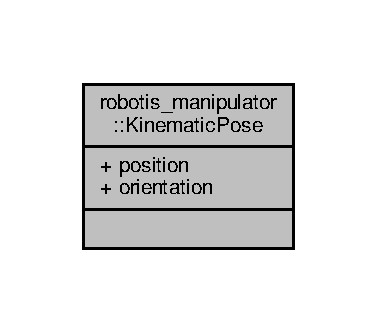
\includegraphics[width=181pt]{structrobotis__manipulator_1_1_kinematic_pose__coll__graph}
\end{center}
\end{figure}
\subsection*{Public Attributes}
\begin{DoxyCompactItemize}
\item 
Eigen\+::\+Vector3d \hyperlink{structrobotis__manipulator_1_1_kinematic_pose_a8700e7ae2388242cf540e884d52fd97a}{position}
\item 
Eigen\+::\+Matrix3d \hyperlink{structrobotis__manipulator_1_1_kinematic_pose_a0506da3cc344d21656fdd1befdd7fa27}{orientation}
\end{DoxyCompactItemize}


\subsection{Detailed Description}


Definition at line 51 of file robotis\+\_\+manipulator\+\_\+common.\+h.



\subsection{Member Data Documentation}
\index{robotis\+\_\+manipulator\+::\+Kinematic\+Pose@{robotis\+\_\+manipulator\+::\+Kinematic\+Pose}!orientation@{orientation}}
\index{orientation@{orientation}!robotis\+\_\+manipulator\+::\+Kinematic\+Pose@{robotis\+\_\+manipulator\+::\+Kinematic\+Pose}}
\subsubsection[{\texorpdfstring{orientation}{orientation}}]{\setlength{\rightskip}{0pt plus 5cm}Eigen\+::\+Matrix3d robotis\+\_\+manipulator\+::\+Kinematic\+Pose\+::orientation}\hypertarget{structrobotis__manipulator_1_1_kinematic_pose_a0506da3cc344d21656fdd1befdd7fa27}{}\label{structrobotis__manipulator_1_1_kinematic_pose_a0506da3cc344d21656fdd1befdd7fa27}


Definition at line 54 of file robotis\+\_\+manipulator\+\_\+common.\+h.

\index{robotis\+\_\+manipulator\+::\+Kinematic\+Pose@{robotis\+\_\+manipulator\+::\+Kinematic\+Pose}!position@{position}}
\index{position@{position}!robotis\+\_\+manipulator\+::\+Kinematic\+Pose@{robotis\+\_\+manipulator\+::\+Kinematic\+Pose}}
\subsubsection[{\texorpdfstring{position}{position}}]{\setlength{\rightskip}{0pt plus 5cm}Eigen\+::\+Vector3d robotis\+\_\+manipulator\+::\+Kinematic\+Pose\+::position}\hypertarget{structrobotis__manipulator_1_1_kinematic_pose_a8700e7ae2388242cf540e884d52fd97a}{}\label{structrobotis__manipulator_1_1_kinematic_pose_a8700e7ae2388242cf540e884d52fd97a}


Definition at line 53 of file robotis\+\_\+manipulator\+\_\+common.\+h.



The documentation for this struct was generated from the following file\+:\begin{DoxyCompactItemize}
\item 
include/robotis\+\_\+manipulator/\hyperlink{robotis__manipulator__common_8h}{robotis\+\_\+manipulator\+\_\+common.\+h}\end{DoxyCompactItemize}

\hypertarget{classrobotis__manipulator_1_1_kinematics}{}\section{robotis\+\_\+manipulator\+:\+:Kinematics Class Reference}
\label{classrobotis__manipulator_1_1_kinematics}\index{robotis\+\_\+manipulator\+::\+Kinematics@{robotis\+\_\+manipulator\+::\+Kinematics}}


The \hyperlink{classrobotis__manipulator_1_1_kinematics}{Kinematics} class.  




{\ttfamily \#include $<$robotis\+\_\+manipulator\+\_\+manager.\+h$>$}



Collaboration diagram for robotis\+\_\+manipulator\+:\+:Kinematics\+:\nopagebreak
\begin{figure}[H]
\begin{center}
\leavevmode
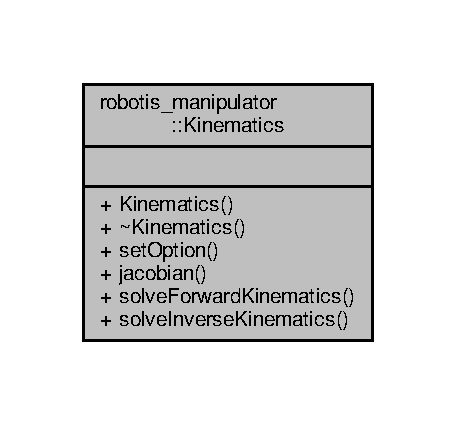
\includegraphics[width=219pt]{classrobotis__manipulator_1_1_kinematics__coll__graph}
\end{center}
\end{figure}
\subsection*{Public Member Functions}
\begin{DoxyCompactItemize}
\item 
\hyperlink{classrobotis__manipulator_1_1_kinematics_a3d08da271bc5cce3cafa2d331277cc5d}{Kinematics} ()
\item 
virtual \hyperlink{classrobotis__manipulator_1_1_kinematics_a202eda8d94a06263cf5d729dd51e59ab}{$\sim$\+Kinematics} ()
\item 
virtual void \hyperlink{classrobotis__manipulator_1_1_kinematics_adc048ff10f7707e3ced3143e583983bc}{set\+Option} (const void $\ast$arg)=0
\begin{DoxyCompactList}\small\item\em set\+Option \end{DoxyCompactList}\item 
virtual Eigen\+::\+Matrix\+Xd \hyperlink{classrobotis__manipulator_1_1_kinematics_a8644b348452df2f0a46b00aadc36c218}{jacobian} (\hyperlink{classrobotis__manipulator_1_1_manipulator}{Manipulator} $\ast$manipulator, \hyperlink{namespacerobotis__manipulator_a08c2d25e77a01ad75b9bb740f8ce4765}{Name} tool\+\_\+name)=0
\begin{DoxyCompactList}\small\item\em jacobian \end{DoxyCompactList}\item 
virtual void \hyperlink{classrobotis__manipulator_1_1_kinematics_adfdd3727052c27d12e3fc2209c025317}{solve\+Forward\+Kinematics} (\hyperlink{classrobotis__manipulator_1_1_manipulator}{Manipulator} $\ast$manipulator)=0
\begin{DoxyCompactList}\small\item\em solve\+Forward\+Kinematics \end{DoxyCompactList}\item 
virtual bool \hyperlink{classrobotis__manipulator_1_1_kinematics_a6065cf1bff763854b9a0bd62945a093b}{solve\+Inverse\+Kinematics} (\hyperlink{classrobotis__manipulator_1_1_manipulator}{Manipulator} $\ast$manipulator, \hyperlink{namespacerobotis__manipulator_a08c2d25e77a01ad75b9bb740f8ce4765}{Name} tool\+\_\+name, \hyperlink{structrobotis__manipulator_1_1_pose}{Pose} target\+\_\+pose, std\+::vector$<$ \hyperlink{namespacerobotis__manipulator_aa0556c98c5294ccf3a96c2d0fe315e40}{Joint\+Value} $>$ $\ast$goal\+\_\+joint\+\_\+position)=0
\begin{DoxyCompactList}\small\item\em solve\+Inverse\+Kinematics \end{DoxyCompactList}\end{DoxyCompactItemize}


\subsection{Detailed Description}
The \hyperlink{classrobotis__manipulator_1_1_kinematics}{Kinematics} class. 

Definition at line 41 of file robotis\+\_\+manipulator\+\_\+manager.\+h.



\subsection{Constructor \& Destructor Documentation}
\index{robotis\+\_\+manipulator\+::\+Kinematics@{robotis\+\_\+manipulator\+::\+Kinematics}!Kinematics@{Kinematics}}
\index{Kinematics@{Kinematics}!robotis\+\_\+manipulator\+::\+Kinematics@{robotis\+\_\+manipulator\+::\+Kinematics}}
\subsubsection[{\texorpdfstring{Kinematics()}{Kinematics()}}]{\setlength{\rightskip}{0pt plus 5cm}robotis\+\_\+manipulator\+::\+Kinematics\+::\+Kinematics (
\begin{DoxyParamCaption}
{}
\end{DoxyParamCaption}
)\hspace{0.3cm}{\ttfamily [inline]}}\hypertarget{classrobotis__manipulator_1_1_kinematics_a3d08da271bc5cce3cafa2d331277cc5d}{}\label{classrobotis__manipulator_1_1_kinematics_a3d08da271bc5cce3cafa2d331277cc5d}


Definition at line 44 of file robotis\+\_\+manipulator\+\_\+manager.\+h.


\begin{DoxyCode}
44 \{\}
\end{DoxyCode}
\index{robotis\+\_\+manipulator\+::\+Kinematics@{robotis\+\_\+manipulator\+::\+Kinematics}!````~Kinematics@{$\sim$\+Kinematics}}
\index{````~Kinematics@{$\sim$\+Kinematics}!robotis\+\_\+manipulator\+::\+Kinematics@{robotis\+\_\+manipulator\+::\+Kinematics}}
\subsubsection[{\texorpdfstring{$\sim$\+Kinematics()}{~Kinematics()}}]{\setlength{\rightskip}{0pt plus 5cm}virtual robotis\+\_\+manipulator\+::\+Kinematics\+::$\sim$\+Kinematics (
\begin{DoxyParamCaption}
{}
\end{DoxyParamCaption}
)\hspace{0.3cm}{\ttfamily [inline]}, {\ttfamily [virtual]}}\hypertarget{classrobotis__manipulator_1_1_kinematics_a202eda8d94a06263cf5d729dd51e59ab}{}\label{classrobotis__manipulator_1_1_kinematics_a202eda8d94a06263cf5d729dd51e59ab}


Definition at line 45 of file robotis\+\_\+manipulator\+\_\+manager.\+h.


\begin{DoxyCode}
45 \{\}
\end{DoxyCode}


Here is the call graph for this function\+:\nopagebreak
\begin{figure}[H]
\begin{center}
\leavevmode
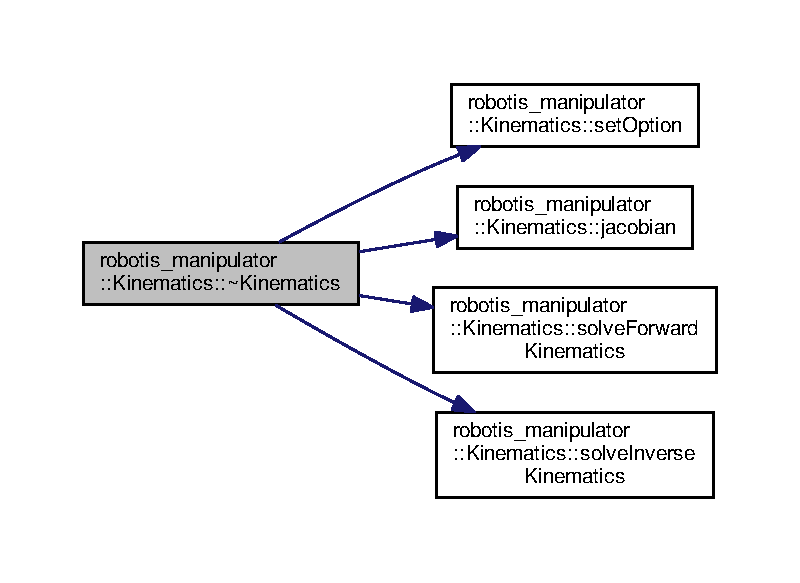
\includegraphics[width=350pt]{classrobotis__manipulator_1_1_kinematics_a202eda8d94a06263cf5d729dd51e59ab_cgraph}
\end{center}
\end{figure}




\subsection{Member Function Documentation}
\index{robotis\+\_\+manipulator\+::\+Kinematics@{robotis\+\_\+manipulator\+::\+Kinematics}!jacobian@{jacobian}}
\index{jacobian@{jacobian}!robotis\+\_\+manipulator\+::\+Kinematics@{robotis\+\_\+manipulator\+::\+Kinematics}}
\subsubsection[{\texorpdfstring{jacobian(\+Manipulator $\ast$manipulator, Name tool\+\_\+name)=0}{jacobian(Manipulator *manipulator, Name tool_name)=0}}]{\setlength{\rightskip}{0pt plus 5cm}virtual Eigen\+::\+Matrix\+Xd robotis\+\_\+manipulator\+::\+Kinematics\+::jacobian (
\begin{DoxyParamCaption}
\item[{{\bf Manipulator} $\ast$}]{manipulator, }
\item[{{\bf Name}}]{tool\+\_\+name}
\end{DoxyParamCaption}
)\hspace{0.3cm}{\ttfamily [pure virtual]}}\hypertarget{classrobotis__manipulator_1_1_kinematics_a8644b348452df2f0a46b00aadc36c218}{}\label{classrobotis__manipulator_1_1_kinematics_a8644b348452df2f0a46b00aadc36c218}


jacobian 


\begin{DoxyParams}{Parameters}
{\em manipulator} & \\
\hline
{\em tool\+\_\+name} & \\
\hline
\end{DoxyParams}
\begin{DoxyReturn}{Returns}

\end{DoxyReturn}


Here is the caller graph for this function\+:\nopagebreak
\begin{figure}[H]
\begin{center}
\leavevmode
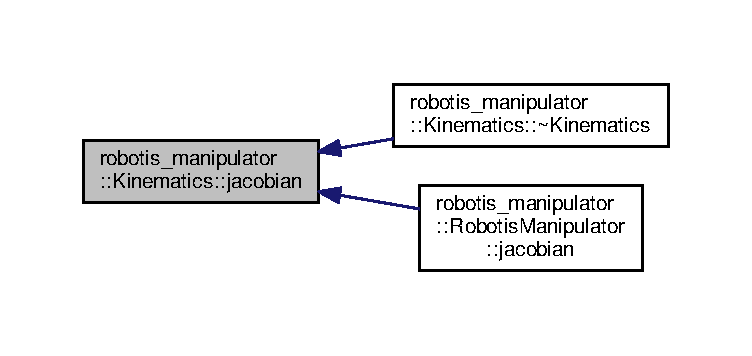
\includegraphics[width=350pt]{classrobotis__manipulator_1_1_kinematics_a8644b348452df2f0a46b00aadc36c218_icgraph}
\end{center}
\end{figure}


\index{robotis\+\_\+manipulator\+::\+Kinematics@{robotis\+\_\+manipulator\+::\+Kinematics}!set\+Option@{set\+Option}}
\index{set\+Option@{set\+Option}!robotis\+\_\+manipulator\+::\+Kinematics@{robotis\+\_\+manipulator\+::\+Kinematics}}
\subsubsection[{\texorpdfstring{set\+Option(const void $\ast$arg)=0}{setOption(const void *arg)=0}}]{\setlength{\rightskip}{0pt plus 5cm}virtual void robotis\+\_\+manipulator\+::\+Kinematics\+::set\+Option (
\begin{DoxyParamCaption}
\item[{const void $\ast$}]{arg}
\end{DoxyParamCaption}
)\hspace{0.3cm}{\ttfamily [pure virtual]}}\hypertarget{classrobotis__manipulator_1_1_kinematics_adc048ff10f7707e3ced3143e583983bc}{}\label{classrobotis__manipulator_1_1_kinematics_adc048ff10f7707e3ced3143e583983bc}


set\+Option 


\begin{DoxyParams}{Parameters}
{\em arg} & \\
\hline
\end{DoxyParams}


Here is the caller graph for this function\+:\nopagebreak
\begin{figure}[H]
\begin{center}
\leavevmode
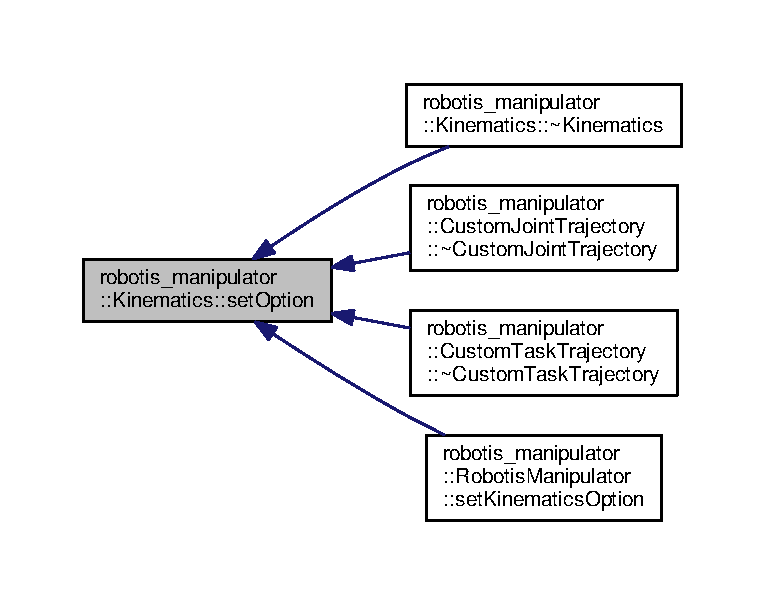
\includegraphics[width=350pt]{classrobotis__manipulator_1_1_kinematics_adc048ff10f7707e3ced3143e583983bc_icgraph}
\end{center}
\end{figure}


\index{robotis\+\_\+manipulator\+::\+Kinematics@{robotis\+\_\+manipulator\+::\+Kinematics}!solve\+Forward\+Kinematics@{solve\+Forward\+Kinematics}}
\index{solve\+Forward\+Kinematics@{solve\+Forward\+Kinematics}!robotis\+\_\+manipulator\+::\+Kinematics@{robotis\+\_\+manipulator\+::\+Kinematics}}
\subsubsection[{\texorpdfstring{solve\+Forward\+Kinematics(\+Manipulator $\ast$manipulator)=0}{solveForwardKinematics(Manipulator *manipulator)=0}}]{\setlength{\rightskip}{0pt plus 5cm}virtual void robotis\+\_\+manipulator\+::\+Kinematics\+::solve\+Forward\+Kinematics (
\begin{DoxyParamCaption}
\item[{{\bf Manipulator} $\ast$}]{manipulator}
\end{DoxyParamCaption}
)\hspace{0.3cm}{\ttfamily [pure virtual]}}\hypertarget{classrobotis__manipulator_1_1_kinematics_adfdd3727052c27d12e3fc2209c025317}{}\label{classrobotis__manipulator_1_1_kinematics_adfdd3727052c27d12e3fc2209c025317}


solve\+Forward\+Kinematics 


\begin{DoxyParams}{Parameters}
{\em manipulator} & \\
\hline
\end{DoxyParams}


Here is the caller graph for this function\+:\nopagebreak
\begin{figure}[H]
\begin{center}
\leavevmode
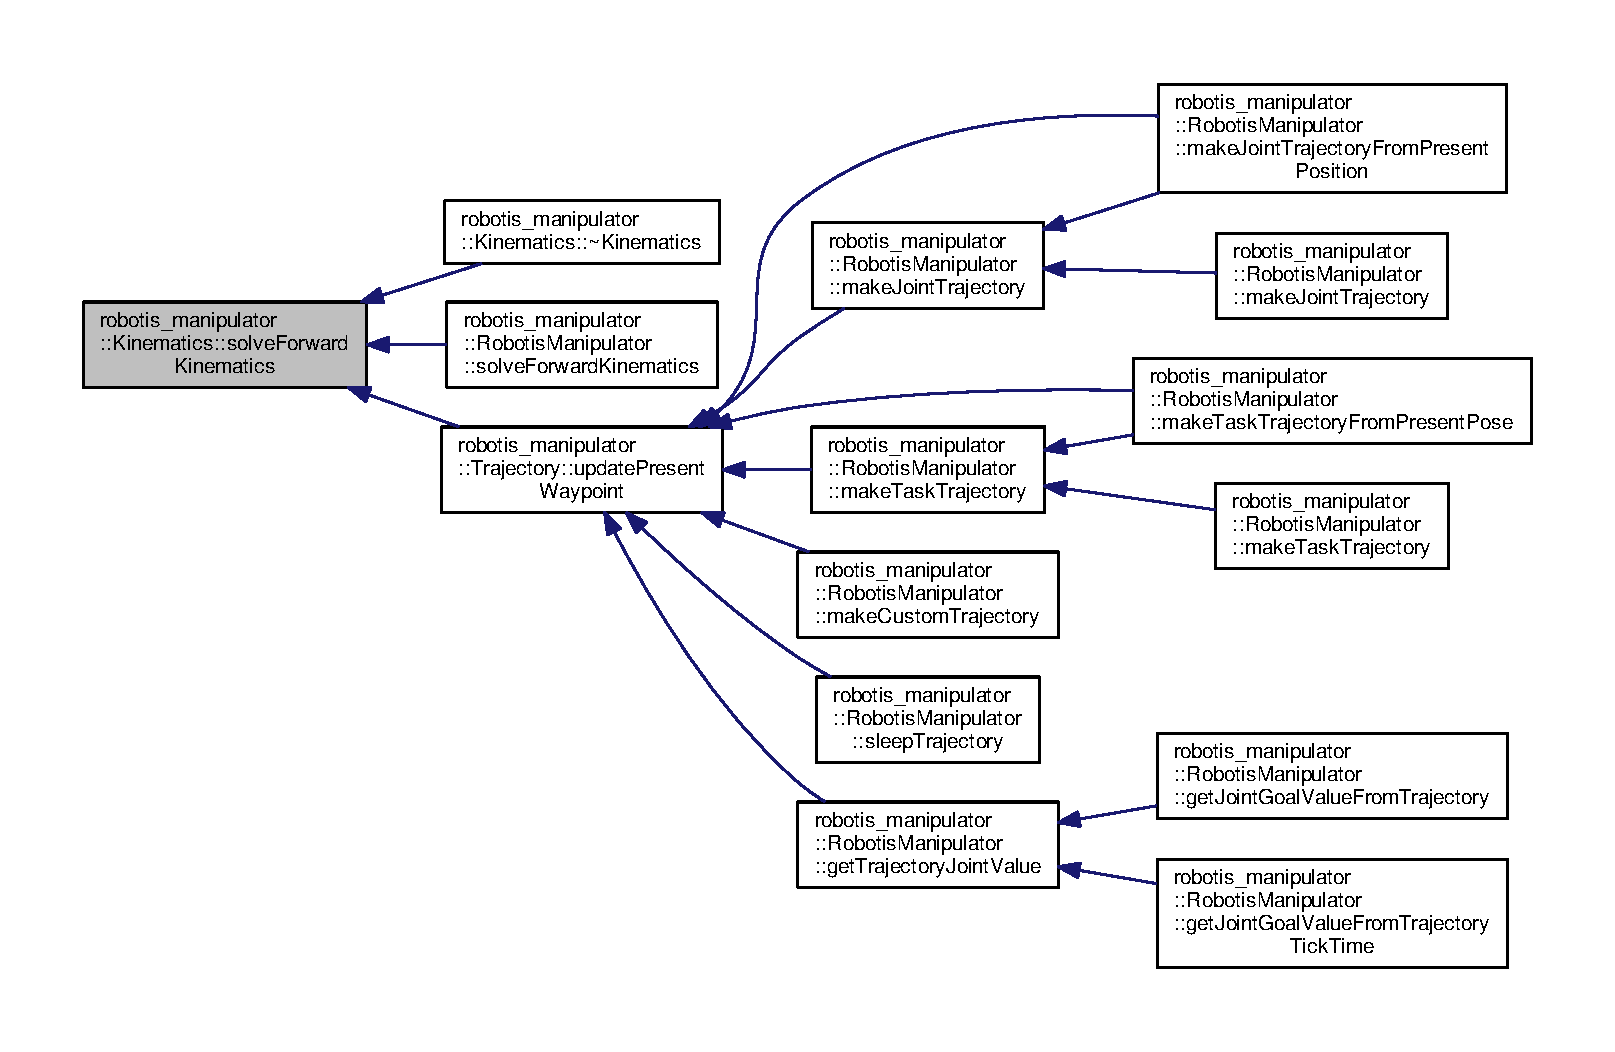
\includegraphics[width=350pt]{classrobotis__manipulator_1_1_kinematics_adfdd3727052c27d12e3fc2209c025317_icgraph}
\end{center}
\end{figure}


\index{robotis\+\_\+manipulator\+::\+Kinematics@{robotis\+\_\+manipulator\+::\+Kinematics}!solve\+Inverse\+Kinematics@{solve\+Inverse\+Kinematics}}
\index{solve\+Inverse\+Kinematics@{solve\+Inverse\+Kinematics}!robotis\+\_\+manipulator\+::\+Kinematics@{robotis\+\_\+manipulator\+::\+Kinematics}}
\subsubsection[{\texorpdfstring{solve\+Inverse\+Kinematics(\+Manipulator $\ast$manipulator, Name tool\+\_\+name, Pose target\+\_\+pose, std\+::vector$<$ Joint\+Value $>$ $\ast$goal\+\_\+joint\+\_\+position)=0}{solveInverseKinematics(Manipulator *manipulator, Name tool_name, Pose target_pose, std::vector< JointValue > *goal_joint_position)=0}}]{\setlength{\rightskip}{0pt plus 5cm}virtual bool robotis\+\_\+manipulator\+::\+Kinematics\+::solve\+Inverse\+Kinematics (
\begin{DoxyParamCaption}
\item[{{\bf Manipulator} $\ast$}]{manipulator, }
\item[{{\bf Name}}]{tool\+\_\+name, }
\item[{{\bf Pose}}]{target\+\_\+pose, }
\item[{std\+::vector$<$ {\bf Joint\+Value} $>$ $\ast$}]{goal\+\_\+joint\+\_\+position}
\end{DoxyParamCaption}
)\hspace{0.3cm}{\ttfamily [pure virtual]}}\hypertarget{classrobotis__manipulator_1_1_kinematics_a6065cf1bff763854b9a0bd62945a093b}{}\label{classrobotis__manipulator_1_1_kinematics_a6065cf1bff763854b9a0bd62945a093b}


solve\+Inverse\+Kinematics 


\begin{DoxyParams}{Parameters}
{\em manipulator} & \\
\hline
{\em tool\+\_\+name} & \\
\hline
{\em target\+\_\+pose} & \\
\hline
{\em goal\+\_\+joint\+\_\+position} & \\
\hline
\end{DoxyParams}
\begin{DoxyReturn}{Returns}

\end{DoxyReturn}


Here is the caller graph for this function\+:\nopagebreak
\begin{figure}[H]
\begin{center}
\leavevmode
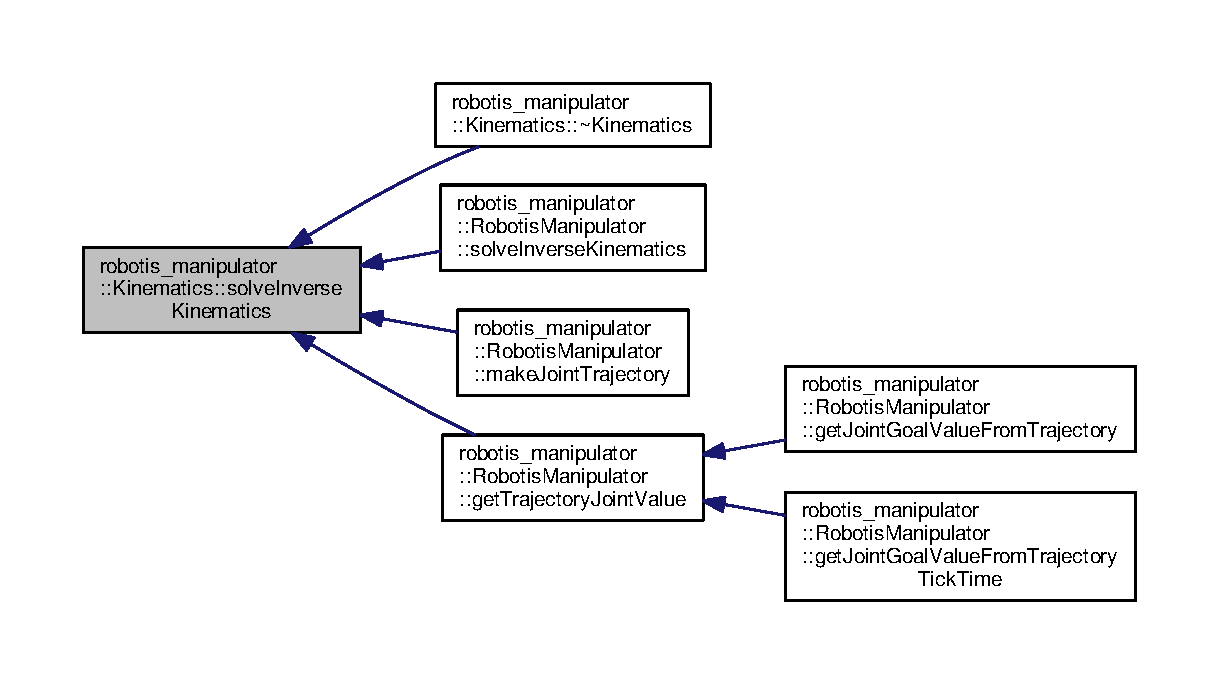
\includegraphics[width=350pt]{classrobotis__manipulator_1_1_kinematics_a6065cf1bff763854b9a0bd62945a093b_icgraph}
\end{center}
\end{figure}




The documentation for this class was generated from the following file\+:\begin{DoxyCompactItemize}
\item 
include/robotis\+\_\+manipulator/\hyperlink{robotis__manipulator__manager_8h}{robotis\+\_\+manipulator\+\_\+manager.\+h}\end{DoxyCompactItemize}

\hypertarget{structrobotis__manipulator_1_1_limit}{}\section{robotis\+\_\+manipulator\+:\+:Limit Struct Reference}
\label{structrobotis__manipulator_1_1_limit}\index{robotis\+\_\+manipulator\+::\+Limit@{robotis\+\_\+manipulator\+::\+Limit}}


{\ttfamily \#include $<$robotis\+\_\+manipulator\+\_\+common.\+h$>$}



Collaboration diagram for robotis\+\_\+manipulator\+:\+:Limit\+:\nopagebreak
\begin{figure}[H]
\begin{center}
\leavevmode
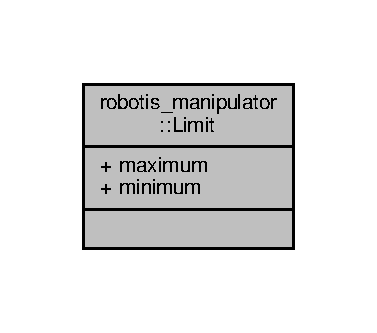
\includegraphics[width=181pt]{structrobotis__manipulator_1_1_limit__coll__graph}
\end{center}
\end{figure}
\subsection*{Public Attributes}
\begin{DoxyCompactItemize}
\item 
double \hyperlink{structrobotis__manipulator_1_1_limit_a82c3d92bd685eb0484fc3ae47f2c3744}{maximum}
\item 
double \hyperlink{structrobotis__manipulator_1_1_limit_ac32cfcc9a4d06728b518e294a0a6030e}{minimum}
\end{DoxyCompactItemize}


\subsection{Detailed Description}


Definition at line 76 of file robotis\+\_\+manipulator\+\_\+common.\+h.



\subsection{Member Data Documentation}
\index{robotis\+\_\+manipulator\+::\+Limit@{robotis\+\_\+manipulator\+::\+Limit}!maximum@{maximum}}
\index{maximum@{maximum}!robotis\+\_\+manipulator\+::\+Limit@{robotis\+\_\+manipulator\+::\+Limit}}
\subsubsection[{\texorpdfstring{maximum}{maximum}}]{\setlength{\rightskip}{0pt plus 5cm}double robotis\+\_\+manipulator\+::\+Limit\+::maximum}\hypertarget{structrobotis__manipulator_1_1_limit_a82c3d92bd685eb0484fc3ae47f2c3744}{}\label{structrobotis__manipulator_1_1_limit_a82c3d92bd685eb0484fc3ae47f2c3744}


Definition at line 78 of file robotis\+\_\+manipulator\+\_\+common.\+h.

\index{robotis\+\_\+manipulator\+::\+Limit@{robotis\+\_\+manipulator\+::\+Limit}!minimum@{minimum}}
\index{minimum@{minimum}!robotis\+\_\+manipulator\+::\+Limit@{robotis\+\_\+manipulator\+::\+Limit}}
\subsubsection[{\texorpdfstring{minimum}{minimum}}]{\setlength{\rightskip}{0pt plus 5cm}double robotis\+\_\+manipulator\+::\+Limit\+::minimum}\hypertarget{structrobotis__manipulator_1_1_limit_ac32cfcc9a4d06728b518e294a0a6030e}{}\label{structrobotis__manipulator_1_1_limit_ac32cfcc9a4d06728b518e294a0a6030e}


Definition at line 79 of file robotis\+\_\+manipulator\+\_\+common.\+h.



The documentation for this struct was generated from the following file\+:\begin{DoxyCompactItemize}
\item 
include/robotis\+\_\+manipulator/\hyperlink{robotis__manipulator__common_8h}{robotis\+\_\+manipulator\+\_\+common.\+h}\end{DoxyCompactItemize}

\hypertarget{classrobotis__manipulator_1_1_manipulator}{}\section{robotis\+\_\+manipulator\+:\+:Manipulator Class Reference}
\label{classrobotis__manipulator_1_1_manipulator}\index{robotis\+\_\+manipulator\+::\+Manipulator@{robotis\+\_\+manipulator\+::\+Manipulator}}


The \hyperlink{classrobotis__manipulator_1_1_manipulator}{Manipulator} class.  




{\ttfamily \#include $<$robotis\+\_\+manipulator\+\_\+common.\+h$>$}



Collaboration diagram for robotis\+\_\+manipulator\+:\+:Manipulator\+:\nopagebreak
\begin{figure}[H]
\begin{center}
\leavevmode
\includegraphics[height=550pt]{classrobotis__manipulator_1_1_manipulator__coll__graph}
\end{center}
\end{figure}
\subsection*{Public Member Functions}
\begin{DoxyCompactItemize}
\item 
\hyperlink{classrobotis__manipulator_1_1_manipulator_a4c301d01641037e7548a1b87e6103f65}{Manipulator} ()
\item 
\hyperlink{classrobotis__manipulator_1_1_manipulator_a90c57c694c00e9380ccd3c399ef85acf}{$\sim$\+Manipulator} ()
\item 
void \hyperlink{classrobotis__manipulator_1_1_manipulator_a703e6d5646e595281d0352c2d0363327}{add\+World} (\hyperlink{namespacerobotis__manipulator_a08c2d25e77a01ad75b9bb740f8ce4765}{Name} world\+\_\+name, \hyperlink{namespacerobotis__manipulator_a08c2d25e77a01ad75b9bb740f8ce4765}{Name} child\+\_\+name, Eigen\+::\+Vector3d world\+\_\+position=Eigen\+::\+Vector3d\+::\+Zero(), Eigen\+::\+Matrix3d world\+\_\+orientation=Eigen\+::\+Matrix3d\+::\+Identity())
\begin{DoxyCompactList}\small\item\em add\+World \end{DoxyCompactList}\item 
void \hyperlink{classrobotis__manipulator_1_1_manipulator_a55c49ab2eb46afd6595ad9de306042b1}{add\+Joint} (\hyperlink{namespacerobotis__manipulator_a08c2d25e77a01ad75b9bb740f8ce4765}{Name} my\+\_\+name, \hyperlink{namespacerobotis__manipulator_a08c2d25e77a01ad75b9bb740f8ce4765}{Name} parent\+\_\+name, \hyperlink{namespacerobotis__manipulator_a08c2d25e77a01ad75b9bb740f8ce4765}{Name} child\+\_\+name, Eigen\+::\+Vector3d relative\+\_\+position, Eigen\+::\+Matrix3d relative\+\_\+orientation, Eigen\+::\+Vector3d axis\+\_\+of\+\_\+rotation=Eigen\+::\+Vector3d\+::\+Zero(), int8\+\_\+t joint\+\_\+actuator\+\_\+id=-\/1, double max\+\_\+position\+\_\+limit=M\+\_\+\+PI, double min\+\_\+position\+\_\+limit=-\/M\+\_\+\+PI, double coefficient=1.\+0, double mass=0.\+0, Eigen\+::\+Matrix3d inertia\+\_\+tensor=Eigen\+::\+Matrix3d\+::\+Identity(), Eigen\+::\+Vector3d center\+\_\+of\+\_\+mass=Eigen\+::\+Vector3d\+::\+Zero())
\begin{DoxyCompactList}\small\item\em add\+Joint \end{DoxyCompactList}\item 
void \hyperlink{classrobotis__manipulator_1_1_manipulator_a55b0500cb070eef28b7c133dacd98d38}{add\+Tool} (\hyperlink{namespacerobotis__manipulator_a08c2d25e77a01ad75b9bb740f8ce4765}{Name} my\+\_\+name, \hyperlink{namespacerobotis__manipulator_a08c2d25e77a01ad75b9bb740f8ce4765}{Name} parent\+\_\+name, Eigen\+::\+Vector3d relative\+\_\+position, Eigen\+::\+Matrix3d relative\+\_\+orientation, int8\+\_\+t tool\+\_\+id=-\/1, double max\+\_\+position\+\_\+limit=M\+\_\+\+PI, double min\+\_\+position\+\_\+limit=-\/M\+\_\+\+PI, double coefficient=1.\+0, double mass=0.\+0, Eigen\+::\+Matrix3d inertia\+\_\+tensor=Eigen\+::\+Matrix3d\+::\+Identity(), Eigen\+::\+Vector3d center\+\_\+of\+\_\+mass=Eigen\+::\+Vector3d\+::\+Zero())
\begin{DoxyCompactList}\small\item\em add\+Tool \end{DoxyCompactList}\item 
void \hyperlink{classrobotis__manipulator_1_1_manipulator_aa26790929f153a49180239f3ac82338f}{add\+Component\+Child} (\hyperlink{namespacerobotis__manipulator_a08c2d25e77a01ad75b9bb740f8ce4765}{Name} my\+\_\+name, \hyperlink{namespacerobotis__manipulator_a08c2d25e77a01ad75b9bb740f8ce4765}{Name} child\+\_\+name)
\begin{DoxyCompactList}\small\item\em add\+Component\+Child \end{DoxyCompactList}\item 
void \hyperlink{classrobotis__manipulator_1_1_manipulator_a4905d7e23cba50ee7c518d078774efe8}{print\+Manipulator\+Setting} ()
\begin{DoxyCompactList}\small\item\em print\+Manipulator\+Setting \end{DoxyCompactList}\item 
void \hyperlink{classrobotis__manipulator_1_1_manipulator_a0a6290aa7c975c78e0d024be9bedd802}{set\+World\+Pose} (\hyperlink{structrobotis__manipulator_1_1_pose}{Pose} world\+\_\+pose)
\begin{DoxyCompactList}\small\item\em set\+World\+Pose \end{DoxyCompactList}\item 
void \hyperlink{classrobotis__manipulator_1_1_manipulator_a2e6c5c86669eff458be6bbd0c960f0cf}{set\+World\+Kinematic\+Pose} (\hyperlink{structrobotis__manipulator_1_1_kinematic_pose}{Kinematic\+Pose} world\+\_\+kinematic\+\_\+pose)
\begin{DoxyCompactList}\small\item\em set\+World\+Kinematic\+Pose \end{DoxyCompactList}\item 
void \hyperlink{classrobotis__manipulator_1_1_manipulator_a7e07c0d513fbac5e758280a3105543d9}{set\+World\+Position} (Eigen\+::\+Vector3d world\+\_\+position)
\begin{DoxyCompactList}\small\item\em set\+World\+Position \end{DoxyCompactList}\item 
void \hyperlink{classrobotis__manipulator_1_1_manipulator_aeb2ca276081f334d2dcdd8808660189d}{set\+World\+Orientation} (Eigen\+::\+Matrix3d world\+\_\+orientation)
\begin{DoxyCompactList}\small\item\em set\+World\+Orientation \end{DoxyCompactList}\item 
void \hyperlink{classrobotis__manipulator_1_1_manipulator_a15476bd6ca87081029c96dd8c6bad319}{set\+World\+Dynamic\+Pose} (\hyperlink{structrobotis__manipulator_1_1_dynamic_pose}{Dynamic\+Pose} world\+\_\+dynamic\+\_\+pose)
\begin{DoxyCompactList}\small\item\em set\+World\+Dynamic\+Pose \end{DoxyCompactList}\item 
void \hyperlink{classrobotis__manipulator_1_1_manipulator_a9d842b9fc11e76aad985b86b4814caf5}{set\+World\+Linear\+Velocity} (Eigen\+::\+Vector3d world\+\_\+linear\+\_\+velocity)
\begin{DoxyCompactList}\small\item\em set\+World\+Linear\+Velocity \end{DoxyCompactList}\item 
void \hyperlink{classrobotis__manipulator_1_1_manipulator_a8fb7188e96d33514a8e5205c79d9b0fc}{set\+World\+Angular\+Velocity} (Eigen\+::\+Vector3d world\+\_\+angular\+\_\+velocity)
\begin{DoxyCompactList}\small\item\em set\+World\+Angular\+Velocity \end{DoxyCompactList}\item 
void \hyperlink{classrobotis__manipulator_1_1_manipulator_a6907a02ab76092769a74f1197bedd381}{set\+World\+Linear\+Acceleration} (Eigen\+::\+Vector3d world\+\_\+linear\+\_\+acceleration)
\begin{DoxyCompactList}\small\item\em set\+World\+Linear\+Acceleration \end{DoxyCompactList}\item 
void \hyperlink{classrobotis__manipulator_1_1_manipulator_a456c183bce6514a5b5c1b1524c5033ac}{set\+World\+Angular\+Acceleration} (Eigen\+::\+Vector3d world\+\_\+angular\+\_\+acceleration)
\begin{DoxyCompactList}\small\item\em set\+World\+Angular\+Acceleration \end{DoxyCompactList}\item 
void \hyperlink{classrobotis__manipulator_1_1_manipulator_a3592945e556a0762c4d306817f3d700f}{set\+Component} (\hyperlink{namespacerobotis__manipulator_a08c2d25e77a01ad75b9bb740f8ce4765}{Name} component\+\_\+name, \hyperlink{structrobotis__manipulator_1_1_component}{Component} component)
\begin{DoxyCompactList}\small\item\em set\+Component \end{DoxyCompactList}\item 
void \hyperlink{classrobotis__manipulator_1_1_manipulator_a27e5f2bca0da521334d59600134bd28b}{set\+Component\+Actuator\+Name} (\hyperlink{namespacerobotis__manipulator_a08c2d25e77a01ad75b9bb740f8ce4765}{Name} component\+\_\+name, \hyperlink{namespacerobotis__manipulator_a08c2d25e77a01ad75b9bb740f8ce4765}{Name} actuator\+\_\+name)
\begin{DoxyCompactList}\small\item\em set\+Component\+Actuator\+Name \end{DoxyCompactList}\item 
void \hyperlink{classrobotis__manipulator_1_1_manipulator_ad070b3aba379f97459e2c784626d05a4}{set\+Component\+Pose\+From\+World} (\hyperlink{namespacerobotis__manipulator_a08c2d25e77a01ad75b9bb740f8ce4765}{Name} component\+\_\+name, \hyperlink{structrobotis__manipulator_1_1_pose}{Pose} pose\+\_\+to\+\_\+world)
\begin{DoxyCompactList}\small\item\em set\+Component\+Pose\+From\+World \end{DoxyCompactList}\item 
void \hyperlink{classrobotis__manipulator_1_1_manipulator_a385fe607bab5200b5898541d4d03a005}{set\+Component\+Kinematic\+Pose\+From\+World} (\hyperlink{namespacerobotis__manipulator_a08c2d25e77a01ad75b9bb740f8ce4765}{Name} component\+\_\+name, \hyperlink{structrobotis__manipulator_1_1_kinematic_pose}{Kinematic\+Pose} pose\+\_\+to\+\_\+world)
\begin{DoxyCompactList}\small\item\em set\+Component\+Kinematic\+Pose\+From\+World \end{DoxyCompactList}\item 
void \hyperlink{classrobotis__manipulator_1_1_manipulator_ab3b7bbd92252755711019606642f83c6}{set\+Component\+Position\+From\+World} (\hyperlink{namespacerobotis__manipulator_a08c2d25e77a01ad75b9bb740f8ce4765}{Name} component\+\_\+name, Eigen\+::\+Vector3d position\+\_\+to\+\_\+world)
\begin{DoxyCompactList}\small\item\em set\+Component\+Position\+From\+World \end{DoxyCompactList}\item 
void \hyperlink{classrobotis__manipulator_1_1_manipulator_a692e8e4bdf8affcfe615f7fc56f1d5f0}{set\+Component\+Orientation\+From\+World} (\hyperlink{namespacerobotis__manipulator_a08c2d25e77a01ad75b9bb740f8ce4765}{Name} component\+\_\+name, Eigen\+::\+Matrix3d orientation\+\_\+to\+\_\+wolrd)
\begin{DoxyCompactList}\small\item\em set\+Component\+Orientation\+From\+World \end{DoxyCompactList}\item 
void \hyperlink{classrobotis__manipulator_1_1_manipulator_a904b6dccb05e5edaae2c7e29d54fd197}{set\+Component\+Dynamic\+Pose\+From\+World} (\hyperlink{namespacerobotis__manipulator_a08c2d25e77a01ad75b9bb740f8ce4765}{Name} component\+\_\+name, \hyperlink{structrobotis__manipulator_1_1_dynamic_pose}{Dynamic\+Pose} dynamic\+\_\+pose)
\begin{DoxyCompactList}\small\item\em set\+Component\+Dynamic\+Pose\+From\+World \end{DoxyCompactList}\item 
void \hyperlink{classrobotis__manipulator_1_1_manipulator_acedaab5099be0997bb2aae307c81fa80}{set\+Joint\+Position} (\hyperlink{namespacerobotis__manipulator_a08c2d25e77a01ad75b9bb740f8ce4765}{Name} name, double position)
\begin{DoxyCompactList}\small\item\em set\+Joint\+Position \end{DoxyCompactList}\item 
void \hyperlink{classrobotis__manipulator_1_1_manipulator_aa8d57910111e9d1ec39313d2527b6c08}{set\+Joint\+Velocity} (\hyperlink{namespacerobotis__manipulator_a08c2d25e77a01ad75b9bb740f8ce4765}{Name} name, double velocity)
\begin{DoxyCompactList}\small\item\em set\+Joint\+Velocity \end{DoxyCompactList}\item 
void \hyperlink{classrobotis__manipulator_1_1_manipulator_a07211b030e35d36d64c620eac5e45f92}{set\+Joint\+Acceleration} (\hyperlink{namespacerobotis__manipulator_a08c2d25e77a01ad75b9bb740f8ce4765}{Name} name, double acceleration)
\begin{DoxyCompactList}\small\item\em set\+Joint\+Acceleration \end{DoxyCompactList}\item 
void \hyperlink{classrobotis__manipulator_1_1_manipulator_aa8b95ee42ecd2e93496f546c144609bf}{set\+Joint\+Effort} (\hyperlink{namespacerobotis__manipulator_a08c2d25e77a01ad75b9bb740f8ce4765}{Name} name, double effort)
\begin{DoxyCompactList}\small\item\em set\+Joint\+Effort \end{DoxyCompactList}\item 
void \hyperlink{classrobotis__manipulator_1_1_manipulator_aa740b17551040520851ec8dc1d619bfe}{set\+Joint\+Value} (\hyperlink{namespacerobotis__manipulator_a08c2d25e77a01ad75b9bb740f8ce4765}{Name} name, \hyperlink{namespacerobotis__manipulator_aa0556c98c5294ccf3a96c2d0fe315e40}{Joint\+Value} joint\+\_\+value)
\begin{DoxyCompactList}\small\item\em set\+Joint\+Value \end{DoxyCompactList}\item 
void \hyperlink{classrobotis__manipulator_1_1_manipulator_a5c1a45efe548837cfa8bb51ccc65a757}{set\+All\+Active\+Joint\+Position} (std\+::vector$<$ double $>$ joint\+\_\+position\+\_\+vector)
\begin{DoxyCompactList}\small\item\em set\+All\+Active\+Joint\+Position \end{DoxyCompactList}\item 
void \hyperlink{classrobotis__manipulator_1_1_manipulator_af42c8e7d8b0a1fe505832d632348e804}{set\+All\+Active\+Joint\+Value} (std\+::vector$<$ \hyperlink{namespacerobotis__manipulator_aa0556c98c5294ccf3a96c2d0fe315e40}{Joint\+Value} $>$ joint\+\_\+value\+\_\+vector)
\begin{DoxyCompactList}\small\item\em set\+All\+Active\+Joint\+Value \end{DoxyCompactList}\item 
void \hyperlink{classrobotis__manipulator_1_1_manipulator_a5752ed8828468e7a6f729871ff812205}{set\+All\+Joint\+Position} (std\+::vector$<$ double $>$ joint\+\_\+position\+\_\+vector)
\begin{DoxyCompactList}\small\item\em set\+All\+Joint\+Position \end{DoxyCompactList}\item 
void \hyperlink{classrobotis__manipulator_1_1_manipulator_a383388a3c388fbfc4482f670d5e4ad10}{set\+All\+Joint\+Value} (std\+::vector$<$ \hyperlink{namespacerobotis__manipulator_aa0556c98c5294ccf3a96c2d0fe315e40}{Joint\+Value} $>$ joint\+\_\+value\+\_\+vector)
\begin{DoxyCompactList}\small\item\em set\+All\+Joint\+Value \end{DoxyCompactList}\item 
void \hyperlink{classrobotis__manipulator_1_1_manipulator_a1ef41a8b1c12d416646fd0291f66ea81}{set\+All\+Tool\+Position} (std\+::vector$<$ double $>$ tool\+\_\+position\+\_\+vector)
\begin{DoxyCompactList}\small\item\em set\+All\+Tool\+Position \end{DoxyCompactList}\item 
void \hyperlink{classrobotis__manipulator_1_1_manipulator_aea664539cecc8a68c7d58ccbf9760787}{set\+All\+Tool\+Value} (std\+::vector$<$ \hyperlink{namespacerobotis__manipulator_aa0556c98c5294ccf3a96c2d0fe315e40}{Joint\+Value} $>$ tool\+\_\+value\+\_\+vector)
\begin{DoxyCompactList}\small\item\em set\+All\+Tool\+Value \end{DoxyCompactList}\item 
int8\+\_\+t \hyperlink{classrobotis__manipulator_1_1_manipulator_a2be640cd5d1fb496f5a6ccd2bb29d781}{get\+D\+OF} ()
\begin{DoxyCompactList}\small\item\em get\+D\+OF \end{DoxyCompactList}\item 
\hyperlink{namespacerobotis__manipulator_a08c2d25e77a01ad75b9bb740f8ce4765}{Name} \hyperlink{classrobotis__manipulator_1_1_manipulator_a3b070bf112ee69b8982eaae8deb30572}{get\+World\+Name} ()
\begin{DoxyCompactList}\small\item\em get\+World\+Name \end{DoxyCompactList}\item 
\hyperlink{namespacerobotis__manipulator_a08c2d25e77a01ad75b9bb740f8ce4765}{Name} \hyperlink{classrobotis__manipulator_1_1_manipulator_a628177e105b1321f4e52a2ae8dffa9a2}{get\+World\+Child\+Name} ()
\begin{DoxyCompactList}\small\item\em get\+World\+Child\+Name \end{DoxyCompactList}\item 
\hyperlink{structrobotis__manipulator_1_1_pose}{Pose} \hyperlink{classrobotis__manipulator_1_1_manipulator_a479f098004c0c5159d43167f77f3e042}{get\+World\+Pose} ()
\begin{DoxyCompactList}\small\item\em get\+World\+Pose \end{DoxyCompactList}\item 
\hyperlink{structrobotis__manipulator_1_1_kinematic_pose}{Kinematic\+Pose} \hyperlink{classrobotis__manipulator_1_1_manipulator_a0f6de4e9c426d25e6f8dd796a7fa7e67}{get\+World\+Kinematic\+Pose} ()
\begin{DoxyCompactList}\small\item\em get\+World\+Kinematic\+Pose \end{DoxyCompactList}\item 
Eigen\+::\+Vector3d \hyperlink{classrobotis__manipulator_1_1_manipulator_a1a06d64bbc395207454a949fa297690d}{get\+World\+Position} ()
\begin{DoxyCompactList}\small\item\em get\+World\+Position \end{DoxyCompactList}\item 
Eigen\+::\+Matrix3d \hyperlink{classrobotis__manipulator_1_1_manipulator_a01ce8a2bf764dc82c5db428fbed8c078}{get\+World\+Orientation} ()
\begin{DoxyCompactList}\small\item\em get\+World\+Orientation \end{DoxyCompactList}\item 
\hyperlink{structrobotis__manipulator_1_1_dynamic_pose}{Dynamic\+Pose} \hyperlink{classrobotis__manipulator_1_1_manipulator_a8ecb51f08b72848c6471b8ca1aae7306}{get\+World\+Dynamic\+Pose} ()
\begin{DoxyCompactList}\small\item\em get\+World\+Dynamic\+Pose \end{DoxyCompactList}\item 
int8\+\_\+t \hyperlink{classrobotis__manipulator_1_1_manipulator_a2bf9733c62dc10fffce7756d7c2761ec}{get\+Component\+Size} ()
\begin{DoxyCompactList}\small\item\em get\+Component\+Size \end{DoxyCompactList}\item 
std\+::map$<$ \hyperlink{namespacerobotis__manipulator_a08c2d25e77a01ad75b9bb740f8ce4765}{Name}, \hyperlink{structrobotis__manipulator_1_1_component}{Component} $>$ \hyperlink{classrobotis__manipulator_1_1_manipulator_ad15f38d8421fd4ce11ca71527475bbaf}{get\+All\+Component} ()
\begin{DoxyCompactList}\small\item\em get\+All\+Component \end{DoxyCompactList}\item 
std\+::map$<$ \hyperlink{namespacerobotis__manipulator_a08c2d25e77a01ad75b9bb740f8ce4765}{Name}, \hyperlink{structrobotis__manipulator_1_1_component}{Component} $>$\+::iterator \hyperlink{classrobotis__manipulator_1_1_manipulator_a83e1adbb8c496ebf785311c8aab2b9ad}{get\+Iterator\+Begin} ()
\begin{DoxyCompactList}\small\item\em get\+Iterator\+Begin \end{DoxyCompactList}\item 
std\+::map$<$ \hyperlink{namespacerobotis__manipulator_a08c2d25e77a01ad75b9bb740f8ce4765}{Name}, \hyperlink{structrobotis__manipulator_1_1_component}{Component} $>$\+::iterator \hyperlink{classrobotis__manipulator_1_1_manipulator_ae600869bf358724f53241eb5f061ea78}{get\+Iterator\+End} ()
\begin{DoxyCompactList}\small\item\em get\+Iterator\+End \end{DoxyCompactList}\item 
\hyperlink{structrobotis__manipulator_1_1_component}{Component} \hyperlink{classrobotis__manipulator_1_1_manipulator_a38623495d8fb45236c6acf119f388abf}{get\+Component} (\hyperlink{namespacerobotis__manipulator_a08c2d25e77a01ad75b9bb740f8ce4765}{Name} component\+\_\+name)
\begin{DoxyCompactList}\small\item\em get\+Component \end{DoxyCompactList}\item 
\hyperlink{namespacerobotis__manipulator_a08c2d25e77a01ad75b9bb740f8ce4765}{Name} \hyperlink{classrobotis__manipulator_1_1_manipulator_a371446cbf4d2d5a572b173d713305fb1}{get\+Component\+Actuator\+Name} (\hyperlink{namespacerobotis__manipulator_a08c2d25e77a01ad75b9bb740f8ce4765}{Name} component\+\_\+name)
\begin{DoxyCompactList}\small\item\em get\+Component\+Actuator\+Name \end{DoxyCompactList}\item 
\hyperlink{namespacerobotis__manipulator_a08c2d25e77a01ad75b9bb740f8ce4765}{Name} \hyperlink{classrobotis__manipulator_1_1_manipulator_aa1401774b97703aead9174595742b7bd}{get\+Component\+Parent\+Name} (\hyperlink{namespacerobotis__manipulator_a08c2d25e77a01ad75b9bb740f8ce4765}{Name} component\+\_\+name)
\begin{DoxyCompactList}\small\item\em get\+Component\+Parent\+Name \end{DoxyCompactList}\item 
std\+::vector$<$ \hyperlink{namespacerobotis__manipulator_a08c2d25e77a01ad75b9bb740f8ce4765}{Name} $>$ \hyperlink{classrobotis__manipulator_1_1_manipulator_a21d1f387435215c3675517581cf225dd}{get\+Component\+Child\+Name} (\hyperlink{namespacerobotis__manipulator_a08c2d25e77a01ad75b9bb740f8ce4765}{Name} component\+\_\+name)
\begin{DoxyCompactList}\small\item\em get\+Component\+Child\+Name \end{DoxyCompactList}\item 
\hyperlink{structrobotis__manipulator_1_1_pose}{Pose} \hyperlink{classrobotis__manipulator_1_1_manipulator_ae48083e42b02bbf672f43b2f77979f21}{get\+Component\+Pose\+From\+World} (\hyperlink{namespacerobotis__manipulator_a08c2d25e77a01ad75b9bb740f8ce4765}{Name} component\+\_\+name)
\begin{DoxyCompactList}\small\item\em get\+Component\+Pose\+From\+World \end{DoxyCompactList}\item 
\hyperlink{structrobotis__manipulator_1_1_kinematic_pose}{Kinematic\+Pose} \hyperlink{classrobotis__manipulator_1_1_manipulator_abf86af18bdea1094c29763366167bfd5}{get\+Component\+Kinematic\+Pose\+From\+World} (\hyperlink{namespacerobotis__manipulator_a08c2d25e77a01ad75b9bb740f8ce4765}{Name} component\+\_\+name)
\begin{DoxyCompactList}\small\item\em get\+Component\+Kinematic\+Pose\+From\+World \end{DoxyCompactList}\item 
Eigen\+::\+Vector3d \hyperlink{classrobotis__manipulator_1_1_manipulator_a04b2efdf66bc0e4bd04dc9aafd9f2d47}{get\+Component\+Position\+From\+World} (\hyperlink{namespacerobotis__manipulator_a08c2d25e77a01ad75b9bb740f8ce4765}{Name} component\+\_\+name)
\begin{DoxyCompactList}\small\item\em get\+Component\+Position\+From\+World \end{DoxyCompactList}\item 
Eigen\+::\+Matrix3d \hyperlink{classrobotis__manipulator_1_1_manipulator_a9228f1f4b7fd627da2a618b79b2f0c0b}{get\+Component\+Orientation\+From\+World} (\hyperlink{namespacerobotis__manipulator_a08c2d25e77a01ad75b9bb740f8ce4765}{Name} component\+\_\+name)
\begin{DoxyCompactList}\small\item\em get\+Component\+Orientation\+From\+World \end{DoxyCompactList}\item 
\hyperlink{structrobotis__manipulator_1_1_dynamic_pose}{Dynamic\+Pose} \hyperlink{classrobotis__manipulator_1_1_manipulator_abebe232d3d0f532920d38194296733bf}{get\+Component\+Dynamic\+Pose\+From\+World} (\hyperlink{namespacerobotis__manipulator_a08c2d25e77a01ad75b9bb740f8ce4765}{Name} component\+\_\+name)
\begin{DoxyCompactList}\small\item\em get\+Component\+Dynamic\+Pose\+From\+World \end{DoxyCompactList}\item 
\hyperlink{structrobotis__manipulator_1_1_kinematic_pose}{Kinematic\+Pose} \hyperlink{classrobotis__manipulator_1_1_manipulator_a2abc1041fd276bedc98c3a4e4fe4a452}{get\+Component\+Relative\+Pose\+From\+Parent} (\hyperlink{namespacerobotis__manipulator_a08c2d25e77a01ad75b9bb740f8ce4765}{Name} component\+\_\+name)
\begin{DoxyCompactList}\small\item\em get\+Component\+Relative\+Pose\+From\+Parent \end{DoxyCompactList}\item 
Eigen\+::\+Vector3d \hyperlink{classrobotis__manipulator_1_1_manipulator_aa910d1dae2cd9e44be612be1c45d9972}{get\+Component\+Relative\+Position\+From\+Parent} (\hyperlink{namespacerobotis__manipulator_a08c2d25e77a01ad75b9bb740f8ce4765}{Name} component\+\_\+name)
\begin{DoxyCompactList}\small\item\em get\+Component\+Relative\+Position\+From\+Parent \end{DoxyCompactList}\item 
Eigen\+::\+Matrix3d \hyperlink{classrobotis__manipulator_1_1_manipulator_a853cca36072acd6285a51f1df06b68bb}{get\+Component\+Relative\+Orientation\+From\+Parent} (\hyperlink{namespacerobotis__manipulator_a08c2d25e77a01ad75b9bb740f8ce4765}{Name} component\+\_\+name)
\begin{DoxyCompactList}\small\item\em get\+Component\+Relative\+Orientation\+From\+Parent \end{DoxyCompactList}\item 
int8\+\_\+t \hyperlink{classrobotis__manipulator_1_1_manipulator_a60db34ef6a62e0b15aa36f9b1571640d}{get\+Id} (\hyperlink{namespacerobotis__manipulator_a08c2d25e77a01ad75b9bb740f8ce4765}{Name} component\+\_\+name)
\begin{DoxyCompactList}\small\item\em get\+Id \end{DoxyCompactList}\item 
double \hyperlink{classrobotis__manipulator_1_1_manipulator_a437ac5f137aa788c4db07690c185e9ba}{get\+Coefficient} (\hyperlink{namespacerobotis__manipulator_a08c2d25e77a01ad75b9bb740f8ce4765}{Name} component\+\_\+name)
\begin{DoxyCompactList}\small\item\em get\+Coefficient \end{DoxyCompactList}\item 
Eigen\+::\+Vector3d \hyperlink{classrobotis__manipulator_1_1_manipulator_a87ccf9e102541d37ef93f3952a1d2ac9}{get\+Axis} (\hyperlink{namespacerobotis__manipulator_a08c2d25e77a01ad75b9bb740f8ce4765}{Name} component\+\_\+name)
\begin{DoxyCompactList}\small\item\em get\+Axis \end{DoxyCompactList}\item 
double \hyperlink{classrobotis__manipulator_1_1_manipulator_af7c65103032ba25d26dd77b49f7875ec}{get\+Joint\+Position} (\hyperlink{namespacerobotis__manipulator_a08c2d25e77a01ad75b9bb740f8ce4765}{Name} component\+\_\+name)
\begin{DoxyCompactList}\small\item\em get\+Joint\+Position \end{DoxyCompactList}\item 
double \hyperlink{classrobotis__manipulator_1_1_manipulator_a4588f79a86a8bc9505b257f8f4d9b1c4}{get\+Joint\+Velocity} (\hyperlink{namespacerobotis__manipulator_a08c2d25e77a01ad75b9bb740f8ce4765}{Name} component\+\_\+name)
\begin{DoxyCompactList}\small\item\em get\+Joint\+Velocity \end{DoxyCompactList}\item 
double \hyperlink{classrobotis__manipulator_1_1_manipulator_a473427796d0109cd5c093019e5286570}{get\+Joint\+Acceleration} (\hyperlink{namespacerobotis__manipulator_a08c2d25e77a01ad75b9bb740f8ce4765}{Name} component\+\_\+name)
\begin{DoxyCompactList}\small\item\em get\+Joint\+Acceleration \end{DoxyCompactList}\item 
double \hyperlink{classrobotis__manipulator_1_1_manipulator_ae592931354a1bb5f1ee1c14509bd1e5f}{get\+Joint\+Effort} (\hyperlink{namespacerobotis__manipulator_a08c2d25e77a01ad75b9bb740f8ce4765}{Name} component\+\_\+name)
\begin{DoxyCompactList}\small\item\em get\+Joint\+Effort \end{DoxyCompactList}\item 
\hyperlink{namespacerobotis__manipulator_aa0556c98c5294ccf3a96c2d0fe315e40}{Joint\+Value} \hyperlink{classrobotis__manipulator_1_1_manipulator_ad8709ca99c7a1ac09450fc8bca0ab7a5}{get\+Joint\+Value} (\hyperlink{namespacerobotis__manipulator_a08c2d25e77a01ad75b9bb740f8ce4765}{Name} component\+\_\+name)
\begin{DoxyCompactList}\small\item\em get\+Joint\+Value \end{DoxyCompactList}\item 
double \hyperlink{classrobotis__manipulator_1_1_manipulator_a3af8d42e8d3ef45ccbbfc7b052c51e07}{get\+Component\+Mass} (\hyperlink{namespacerobotis__manipulator_a08c2d25e77a01ad75b9bb740f8ce4765}{Name} component\+\_\+name)
\begin{DoxyCompactList}\small\item\em get\+Component\+Mass \end{DoxyCompactList}\item 
Eigen\+::\+Matrix3d \hyperlink{classrobotis__manipulator_1_1_manipulator_a05d58cf6a4e7540d00a8621f9ba83f07}{get\+Component\+Inertia\+Tensor} (\hyperlink{namespacerobotis__manipulator_a08c2d25e77a01ad75b9bb740f8ce4765}{Name} component\+\_\+name)
\begin{DoxyCompactList}\small\item\em get\+Component\+Inertia\+Tensor \end{DoxyCompactList}\item 
Eigen\+::\+Vector3d \hyperlink{classrobotis__manipulator_1_1_manipulator_a7002f6083a3f72754189c60d9e92241a}{get\+Component\+Center\+Of\+Mass} (\hyperlink{namespacerobotis__manipulator_a08c2d25e77a01ad75b9bb740f8ce4765}{Name} component\+\_\+name)
\begin{DoxyCompactList}\small\item\em get\+Component\+Center\+Of\+Mass \end{DoxyCompactList}\item 
std\+::vector$<$ double $>$ \hyperlink{classrobotis__manipulator_1_1_manipulator_a32a7e8ec9292d714fe824982f2f21c83}{get\+All\+Joint\+Position} ()
\begin{DoxyCompactList}\small\item\em get\+All\+Joint\+Position \end{DoxyCompactList}\item 
std\+::vector$<$ \hyperlink{namespacerobotis__manipulator_aa0556c98c5294ccf3a96c2d0fe315e40}{Joint\+Value} $>$ \hyperlink{classrobotis__manipulator_1_1_manipulator_a2d1613d98d3f2bfcddf78df3871ef974}{get\+All\+Joint\+Value} ()
\begin{DoxyCompactList}\small\item\em get\+All\+Joint\+Value \end{DoxyCompactList}\item 
std\+::vector$<$ double $>$ \hyperlink{classrobotis__manipulator_1_1_manipulator_a5910fd02cefde8b34e7db6af4ab8415d}{get\+All\+Active\+Joint\+Position} ()
\begin{DoxyCompactList}\small\item\em get\+All\+Active\+Joint\+Position \end{DoxyCompactList}\item 
std\+::vector$<$ \hyperlink{namespacerobotis__manipulator_aa0556c98c5294ccf3a96c2d0fe315e40}{Joint\+Value} $>$ \hyperlink{classrobotis__manipulator_1_1_manipulator_ae11f05005b456e13ef17585a70179dce}{get\+All\+Active\+Joint\+Value} ()
\begin{DoxyCompactList}\small\item\em get\+All\+Active\+Joint\+Value \end{DoxyCompactList}\item 
std\+::vector$<$ double $>$ \hyperlink{classrobotis__manipulator_1_1_manipulator_af3ed7fd19820970d246f4a2459151075}{get\+All\+Tool\+Position} ()
\begin{DoxyCompactList}\small\item\em get\+All\+Tool\+Position \end{DoxyCompactList}\item 
std\+::vector$<$ \hyperlink{namespacerobotis__manipulator_aa0556c98c5294ccf3a96c2d0fe315e40}{Joint\+Value} $>$ \hyperlink{classrobotis__manipulator_1_1_manipulator_a996f60dc81526d473a3e5223d58979c7}{get\+All\+Tool\+Value} ()
\begin{DoxyCompactList}\small\item\em get\+All\+Tool\+Value \end{DoxyCompactList}\item 
std\+::vector$<$ uint8\+\_\+t $>$ \hyperlink{classrobotis__manipulator_1_1_manipulator_a689daa284722f6b940e1196dd3dde43e}{get\+All\+Joint\+ID} ()
\begin{DoxyCompactList}\small\item\em get\+All\+Joint\+ID \end{DoxyCompactList}\item 
std\+::vector$<$ uint8\+\_\+t $>$ \hyperlink{classrobotis__manipulator_1_1_manipulator_a36d90688599cbd3067ce1d0c07f514aa}{get\+All\+Active\+Joint\+ID} ()
\begin{DoxyCompactList}\small\item\em get\+All\+Active\+Joint\+ID \end{DoxyCompactList}\item 
std\+::vector$<$ \hyperlink{namespacerobotis__manipulator_a08c2d25e77a01ad75b9bb740f8ce4765}{Name} $>$ \hyperlink{classrobotis__manipulator_1_1_manipulator_a53cf6f3195057072869795ebac3b8dce}{get\+All\+Tool\+Component\+Name} ()
\begin{DoxyCompactList}\small\item\em get\+All\+Tool\+Component\+Name \end{DoxyCompactList}\item 
std\+::vector$<$ \hyperlink{namespacerobotis__manipulator_a08c2d25e77a01ad75b9bb740f8ce4765}{Name} $>$ \hyperlink{classrobotis__manipulator_1_1_manipulator_af746f90412f3a1f08dee32a855ca177c}{get\+All\+Active\+Joint\+Component\+Name} ()
\begin{DoxyCompactList}\small\item\em get\+All\+Active\+Joint\+Component\+Name \end{DoxyCompactList}\item 
bool \hyperlink{classrobotis__manipulator_1_1_manipulator_a715e5825f289765d1c6ce9687ce6c6e5}{check\+Joint\+Limit} (\hyperlink{namespacerobotis__manipulator_a08c2d25e77a01ad75b9bb740f8ce4765}{Name} Component\+\_\+name, double value)
\begin{DoxyCompactList}\small\item\em check\+Joint\+Limit \end{DoxyCompactList}\item 
bool \hyperlink{classrobotis__manipulator_1_1_manipulator_a5b1f27b9cc2875b4e0275e3b88ab1b28}{check\+Component\+Type} (\hyperlink{namespacerobotis__manipulator_a08c2d25e77a01ad75b9bb740f8ce4765}{Name} component\+\_\+name, \hyperlink{namespacerobotis__manipulator_a2bbf89d1c08dc1d9ff4e28beb939e382}{Component\+Type} component\+\_\+type)
\begin{DoxyCompactList}\small\item\em check\+Component\+Type \end{DoxyCompactList}\item 
\hyperlink{namespacerobotis__manipulator_a08c2d25e77a01ad75b9bb740f8ce4765}{Name} \hyperlink{classrobotis__manipulator_1_1_manipulator_a9f8406b7a5be743cc2dfc29a9f7ea647}{find\+Component\+Name\+Using\+Id} (int8\+\_\+t id)
\begin{DoxyCompactList}\small\item\em find\+Component\+Name\+Using\+Id \end{DoxyCompactList}\end{DoxyCompactItemize}
\subsection*{Private Attributes}
\begin{DoxyCompactItemize}
\item 
int8\+\_\+t \hyperlink{classrobotis__manipulator_1_1_manipulator_a39092ac588acd5e8713b55e18b85aebb}{dof\+\_\+}
\item 
\hyperlink{structrobotis__manipulator_1_1_world}{World} \hyperlink{classrobotis__manipulator_1_1_manipulator_a2da05841bad220ca4072a11649777bb6}{world\+\_\+}
\item 
std\+::map$<$ \hyperlink{namespacerobotis__manipulator_a08c2d25e77a01ad75b9bb740f8ce4765}{Name}, \hyperlink{structrobotis__manipulator_1_1_component}{Component} $>$ \hyperlink{classrobotis__manipulator_1_1_manipulator_a20b388b821f161972c2cf737fe1c26db}{component\+\_\+}
\end{DoxyCompactItemize}


\subsection{Detailed Description}
The \hyperlink{classrobotis__manipulator_1_1_manipulator}{Manipulator} class. 

Definition at line 183 of file robotis\+\_\+manipulator\+\_\+common.\+h.



\subsection{Constructor \& Destructor Documentation}
\index{robotis\+\_\+manipulator\+::\+Manipulator@{robotis\+\_\+manipulator\+::\+Manipulator}!Manipulator@{Manipulator}}
\index{Manipulator@{Manipulator}!robotis\+\_\+manipulator\+::\+Manipulator@{robotis\+\_\+manipulator\+::\+Manipulator}}
\subsubsection[{\texorpdfstring{Manipulator()}{Manipulator()}}]{\setlength{\rightskip}{0pt plus 5cm}Manipulator\+::\+Manipulator (
\begin{DoxyParamCaption}
{}
\end{DoxyParamCaption}
)}\hypertarget{classrobotis__manipulator_1_1_manipulator_a4c301d01641037e7548a1b87e6103f65}{}\label{classrobotis__manipulator_1_1_manipulator_a4c301d01641037e7548a1b87e6103f65}


Definition at line 30 of file robotis\+\_\+manipulator\+\_\+common.\+cpp.


\begin{DoxyCode}
30 :\hyperlink{classrobotis__manipulator_1_1_manipulator_a39092ac588acd5e8713b55e18b85aebb}{dof\_}(0)\{\}
\end{DoxyCode}
\index{robotis\+\_\+manipulator\+::\+Manipulator@{robotis\+\_\+manipulator\+::\+Manipulator}!````~Manipulator@{$\sim$\+Manipulator}}
\index{````~Manipulator@{$\sim$\+Manipulator}!robotis\+\_\+manipulator\+::\+Manipulator@{robotis\+\_\+manipulator\+::\+Manipulator}}
\subsubsection[{\texorpdfstring{$\sim$\+Manipulator()}{~Manipulator()}}]{\setlength{\rightskip}{0pt plus 5cm}robotis\+\_\+manipulator\+::\+Manipulator\+::$\sim$\+Manipulator (
\begin{DoxyParamCaption}
{}
\end{DoxyParamCaption}
)\hspace{0.3cm}{\ttfamily [inline]}}\hypertarget{classrobotis__manipulator_1_1_manipulator_a90c57c694c00e9380ccd3c399ef85acf}{}\label{classrobotis__manipulator_1_1_manipulator_a90c57c694c00e9380ccd3c399ef85acf}


Definition at line 192 of file robotis\+\_\+manipulator\+\_\+common.\+h.


\begin{DoxyCode}
192 \{\}
\end{DoxyCode}


\subsection{Member Function Documentation}
\index{robotis\+\_\+manipulator\+::\+Manipulator@{robotis\+\_\+manipulator\+::\+Manipulator}!add\+Component\+Child@{add\+Component\+Child}}
\index{add\+Component\+Child@{add\+Component\+Child}!robotis\+\_\+manipulator\+::\+Manipulator@{robotis\+\_\+manipulator\+::\+Manipulator}}
\subsubsection[{\texorpdfstring{add\+Component\+Child(\+Name my\+\_\+name, Name child\+\_\+name)}{addComponentChild(Name my_name, Name child_name)}}]{\setlength{\rightskip}{0pt plus 5cm}void Manipulator\+::add\+Component\+Child (
\begin{DoxyParamCaption}
\item[{{\bf Name}}]{my\+\_\+name, }
\item[{{\bf Name}}]{child\+\_\+name}
\end{DoxyParamCaption}
)}\hypertarget{classrobotis__manipulator_1_1_manipulator_aa26790929f153a49180239f3ac82338f}{}\label{classrobotis__manipulator_1_1_manipulator_aa26790929f153a49180239f3ac82338f}


add\+Component\+Child 


\begin{DoxyParams}{Parameters}
{\em my\+\_\+name} & \\
\hline
{\em child\+\_\+name} & \\
\hline
\end{DoxyParams}


Definition at line 144 of file robotis\+\_\+manipulator\+\_\+common.\+cpp.


\begin{DoxyCode}
145 \{
146   \hyperlink{classrobotis__manipulator_1_1_manipulator_a20b388b821f161972c2cf737fe1c26db}{component\_}.at(my\_name).name.child.push\_back(child\_name);
147 \}
\end{DoxyCode}


Here is the caller graph for this function\+:\nopagebreak
\begin{figure}[H]
\begin{center}
\leavevmode
\includegraphics[width=350pt]{classrobotis__manipulator_1_1_manipulator_aa26790929f153a49180239f3ac82338f_icgraph}
\end{center}
\end{figure}


\index{robotis\+\_\+manipulator\+::\+Manipulator@{robotis\+\_\+manipulator\+::\+Manipulator}!add\+Joint@{add\+Joint}}
\index{add\+Joint@{add\+Joint}!robotis\+\_\+manipulator\+::\+Manipulator@{robotis\+\_\+manipulator\+::\+Manipulator}}
\subsubsection[{\texorpdfstring{add\+Joint(\+Name my\+\_\+name, Name parent\+\_\+name, Name child\+\_\+name, Eigen\+::\+Vector3d relative\+\_\+position, Eigen\+::\+Matrix3d relative\+\_\+orientation, Eigen\+::\+Vector3d axis\+\_\+of\+\_\+rotation=\+Eigen\+::\+Vector3d\+::\+Zero(), int8\+\_\+t joint\+\_\+actuator\+\_\+id=-\/1, double max\+\_\+position\+\_\+limit=\+M\+\_\+\+P\+I, double min\+\_\+position\+\_\+limit=-\/\+M\+\_\+\+P\+I, double coefficient=1.\+0, double mass=0.\+0, Eigen\+::\+Matrix3d inertia\+\_\+tensor=\+Eigen\+::\+Matrix3d\+::\+Identity(), Eigen\+::\+Vector3d center\+\_\+of\+\_\+mass=\+Eigen\+::\+Vector3d\+::\+Zero())}{addJoint(Name my_name, Name parent_name, Name child_name, Eigen::Vector3d relative_position, Eigen::Matrix3d relative_orientation, Eigen::Vector3d axis_of_rotation=Eigen::Vector3d::Zero(), int8_t joint_actuator_id=-1, double max_position_limit=M_PI, double min_position_limit=-M_PI, double coefficient=1.0, double mass=0.0, Eigen::Matrix3d inertia_tensor=Eigen::Matrix3d::Identity(), Eigen::Vector3d center_of_mass=Eigen::Vector3d::Zero())}}]{\setlength{\rightskip}{0pt plus 5cm}void Manipulator\+::add\+Joint (
\begin{DoxyParamCaption}
\item[{{\bf Name}}]{my\+\_\+name, }
\item[{{\bf Name}}]{parent\+\_\+name, }
\item[{{\bf Name}}]{child\+\_\+name, }
\item[{Eigen\+::\+Vector3d}]{relative\+\_\+position, }
\item[{Eigen\+::\+Matrix3d}]{relative\+\_\+orientation, }
\item[{Eigen\+::\+Vector3d}]{axis\+\_\+of\+\_\+rotation = {\ttfamily Eigen\+:\+:Vector3d\+:\+:Zero()}, }
\item[{int8\+\_\+t}]{joint\+\_\+actuator\+\_\+id = {\ttfamily -\/1}, }
\item[{double}]{max\+\_\+position\+\_\+limit = {\ttfamily M\+\_\+PI}, }
\item[{double}]{min\+\_\+position\+\_\+limit = {\ttfamily -\/M\+\_\+PI}, }
\item[{double}]{coefficient = {\ttfamily 1.0}, }
\item[{double}]{mass = {\ttfamily 0.0}, }
\item[{Eigen\+::\+Matrix3d}]{inertia\+\_\+tensor = {\ttfamily Eigen\+:\+:Matrix3d\+:\+:Identity()}, }
\item[{Eigen\+::\+Vector3d}]{center\+\_\+of\+\_\+mass = {\ttfamily Eigen\+:\+:Vector3d\+:\+:Zero()}}
\end{DoxyParamCaption}
)}\hypertarget{classrobotis__manipulator_1_1_manipulator_a55c49ab2eb46afd6595ad9de306042b1}{}\label{classrobotis__manipulator_1_1_manipulator_a55c49ab2eb46afd6595ad9de306042b1}


add\+Joint 


\begin{DoxyParams}{Parameters}
{\em my\+\_\+name} & \\
\hline
{\em parent\+\_\+name} & \\
\hline
{\em child\+\_\+name} & \\
\hline
{\em relative\+\_\+position} & \\
\hline
{\em relative\+\_\+orientation} & \\
\hline
{\em axis\+\_\+of\+\_\+rotation} & \\
\hline
{\em joint\+\_\+actuator\+\_\+id} & \\
\hline
{\em max\+\_\+position\+\_\+limit} & \\
\hline
{\em min\+\_\+position\+\_\+limit} & \\
\hline
{\em coefficient} & \\
\hline
{\em mass} & \\
\hline
{\em inertia\+\_\+tensor} & \\
\hline
{\em center\+\_\+of\+\_\+mass} & \\
\hline
\end{DoxyParams}


Definition at line 50 of file robotis\+\_\+manipulator\+\_\+common.\+cpp.


\begin{DoxyCode}
63 \{
64   \hyperlink{structrobotis__manipulator_1_1_component}{Component} temp\_component;
65   \textcolor{keywordflow}{if} (joint\_actuator\_id != -1)
66   \{
67     \hyperlink{classrobotis__manipulator_1_1_manipulator_a39092ac588acd5e8713b55e18b85aebb}{dof\_}++;
68     temp\_component.\hyperlink{structrobotis__manipulator_1_1_component_ae597791dc579e168914ac36b66cf6172}{component\_type} = \hyperlink{namespacerobotis__manipulator_a2bbf89d1c08dc1d9ff4e28beb939e382acdf3b34914d1a2a028d882beb96fba7c}{ACTIVE\_JOINT\_COMPONENT};
69   \}
70   \textcolor{keywordflow}{else}
71   \{
72     temp\_component.\hyperlink{structrobotis__manipulator_1_1_component_ae597791dc579e168914ac36b66cf6172}{component\_type} = \hyperlink{namespacerobotis__manipulator_a2bbf89d1c08dc1d9ff4e28beb939e382a48d9e14bdd971b547f0b4bfcbf8588e7}{PASSIVE\_JOINT\_COMPONENT};
73   \}
74 
75   temp\_component.\hyperlink{structrobotis__manipulator_1_1_component_a022aa062d295a3a6b5815a58b74e558f}{name}.\hyperlink{structrobotis__manipulator_1_1_chaining_name_aa5e92a4939b2884e63bee3690f387627}{parent} = parent\_name;
76   temp\_component.\hyperlink{structrobotis__manipulator_1_1_component_a022aa062d295a3a6b5815a58b74e558f}{name}.\hyperlink{structrobotis__manipulator_1_1_chaining_name_a600be40420b93d2d8596d07d7e36fbf2}{child}.push\_back(child\_name);
77   temp\_component.\hyperlink{structrobotis__manipulator_1_1_component_af1b86e91e0f92a214fa9e10464aba08f}{relative}.\hyperlink{structrobotis__manipulator_1_1_relative_a0a5f840d8a1f1f34ebd5e285209a8660}{pose\_from\_parent}.\hyperlink{structrobotis__manipulator_1_1_kinematic_pose_a8700e7ae2388242cf540e884d52fd97a}{position} = relative\_position;
78   temp\_component.\hyperlink{structrobotis__manipulator_1_1_component_af1b86e91e0f92a214fa9e10464aba08f}{relative}.\hyperlink{structrobotis__manipulator_1_1_relative_a0a5f840d8a1f1f34ebd5e285209a8660}{pose\_from\_parent}.\hyperlink{structrobotis__manipulator_1_1_kinematic_pose_a0506da3cc344d21656fdd1befdd7fa27}{orientation} = 
      relative\_orientation;
79   temp\_component.\hyperlink{structrobotis__manipulator_1_1_component_af1b86e91e0f92a214fa9e10464aba08f}{relative}.\hyperlink{structrobotis__manipulator_1_1_relative_ad761bd6e74a48a22dedb93feed45f5db}{inertia}.\hyperlink{structrobotis__manipulator_1_1_inertia_a8e25738415288febca11a62124736bab}{mass} = mass;
80   temp\_component.\hyperlink{structrobotis__manipulator_1_1_component_af1b86e91e0f92a214fa9e10464aba08f}{relative}.\hyperlink{structrobotis__manipulator_1_1_relative_ad761bd6e74a48a22dedb93feed45f5db}{inertia}.\hyperlink{structrobotis__manipulator_1_1_inertia_a61b16b0ad0ac7366fe046b946c04c97e}{inertia\_tensor} = inertia\_tensor;
81   temp\_component.\hyperlink{structrobotis__manipulator_1_1_component_af1b86e91e0f92a214fa9e10464aba08f}{relative}.\hyperlink{structrobotis__manipulator_1_1_relative_ad761bd6e74a48a22dedb93feed45f5db}{inertia}.\hyperlink{structrobotis__manipulator_1_1_inertia_a8d7158602370b1abf0b690a6483376b7}{center\_of\_mass} = center\_of\_mass;
82   temp\_component.\hyperlink{structrobotis__manipulator_1_1_component_a39b967aba5061b7cd4e46c9a18d2e223}{joint\_constant}.\hyperlink{structrobotis__manipulator_1_1_joint_constant_ac4e09e4e2886029c58d6f727e9b1e274}{id} = joint\_actuator\_id;
83   temp\_component.\hyperlink{structrobotis__manipulator_1_1_component_a39b967aba5061b7cd4e46c9a18d2e223}{joint\_constant}.\hyperlink{structrobotis__manipulator_1_1_joint_constant_acd88ff436867374790745f4661b12821}{coefficient} = coefficient;
84   temp\_component.\hyperlink{structrobotis__manipulator_1_1_component_a39b967aba5061b7cd4e46c9a18d2e223}{joint\_constant}.\hyperlink{structrobotis__manipulator_1_1_joint_constant_aa3bf091d44be75bd46e5052fd32fccc6}{axis} = axis\_of\_rotation;
85   temp\_component.\hyperlink{structrobotis__manipulator_1_1_component_a39b967aba5061b7cd4e46c9a18d2e223}{joint\_constant}.\hyperlink{structrobotis__manipulator_1_1_joint_constant_a15c9d0a10c81d861a1d4762b0f9a790d}{position\_limit}.
      \hyperlink{structrobotis__manipulator_1_1_limit_a82c3d92bd685eb0484fc3ae47f2c3744}{maximum} = max\_position\_limit;
86   temp\_component.\hyperlink{structrobotis__manipulator_1_1_component_a39b967aba5061b7cd4e46c9a18d2e223}{joint\_constant}.\hyperlink{structrobotis__manipulator_1_1_joint_constant_a15c9d0a10c81d861a1d4762b0f9a790d}{position\_limit}.
      \hyperlink{structrobotis__manipulator_1_1_limit_ac32cfcc9a4d06728b518e294a0a6030e}{minimum} = min\_position\_limit;
87 
88   temp\_component.\hyperlink{structrobotis__manipulator_1_1_component_a0b28dd5fe885ff8f07d75733d6e777fc}{pose\_from\_world}.\hyperlink{structrobotis__manipulator_1_1_pose_a7215a37d50e62643f1523d3fa40a36e9}{kinematic}.\hyperlink{structrobotis__manipulator_1_1_kinematic_pose_a8700e7ae2388242cf540e884d52fd97a}{position} = Eigen::Vector3d::Zero
      ();
89   temp\_component.\hyperlink{structrobotis__manipulator_1_1_component_a0b28dd5fe885ff8f07d75733d6e777fc}{pose\_from\_world}.\hyperlink{structrobotis__manipulator_1_1_pose_a7215a37d50e62643f1523d3fa40a36e9}{kinematic}.\hyperlink{structrobotis__manipulator_1_1_kinematic_pose_a0506da3cc344d21656fdd1befdd7fa27}{orientation} = 
      Eigen::Matrix3d::Identity();
90   temp\_component.\hyperlink{structrobotis__manipulator_1_1_component_a0b28dd5fe885ff8f07d75733d6e777fc}{pose\_from\_world}.\hyperlink{structrobotis__manipulator_1_1_pose_a8accf10d21933e07ade2728fcccf4ae6}{dynamic}.\hyperlink{structrobotis__manipulator_1_1_dynamic_pose_a45f314d8e2d3f78a4bc9c2aa72f0badc}{linear}.
      \hyperlink{structrobotis__manipulator_1_1_dynamicvector_a6bbccf8316887a8da3cd6aa065f3beac}{velocity} = Eigen::Vector3d::Zero();
91   temp\_component.\hyperlink{structrobotis__manipulator_1_1_component_a0b28dd5fe885ff8f07d75733d6e777fc}{pose\_from\_world}.\hyperlink{structrobotis__manipulator_1_1_pose_a8accf10d21933e07ade2728fcccf4ae6}{dynamic}.\hyperlink{structrobotis__manipulator_1_1_dynamic_pose_a45f314d8e2d3f78a4bc9c2aa72f0badc}{linear}.
      \hyperlink{structrobotis__manipulator_1_1_dynamicvector_afc83eba2d67af4c23150a08824f0f01e}{acceleration} = Eigen::Vector3d::Zero();
92   temp\_component.\hyperlink{structrobotis__manipulator_1_1_component_a0b28dd5fe885ff8f07d75733d6e777fc}{pose\_from\_world}.\hyperlink{structrobotis__manipulator_1_1_pose_a8accf10d21933e07ade2728fcccf4ae6}{dynamic}.\hyperlink{structrobotis__manipulator_1_1_dynamic_pose_a424459b0d1108f1e65594f5d193cbae6}{angular}.
      \hyperlink{structrobotis__manipulator_1_1_dynamicvector_a6bbccf8316887a8da3cd6aa065f3beac}{velocity} = Eigen::Vector3d::Zero();
93   temp\_component.\hyperlink{structrobotis__manipulator_1_1_component_a0b28dd5fe885ff8f07d75733d6e777fc}{pose\_from\_world}.\hyperlink{structrobotis__manipulator_1_1_pose_a8accf10d21933e07ade2728fcccf4ae6}{dynamic}.\hyperlink{structrobotis__manipulator_1_1_dynamic_pose_a424459b0d1108f1e65594f5d193cbae6}{angular}.
      \hyperlink{structrobotis__manipulator_1_1_dynamicvector_afc83eba2d67af4c23150a08824f0f01e}{acceleration} = Eigen::Vector3d::Zero();
94 
95   temp\_component.\hyperlink{structrobotis__manipulator_1_1_component_a06de8406b177d397a1f998fdf9d67d95}{joint\_value}.\hyperlink{structrobotis__manipulator_1_1_point_a0f122386b502d9b316bdead542ed2145}{position} = 0.0;
96   temp\_component.\hyperlink{structrobotis__manipulator_1_1_component_a06de8406b177d397a1f998fdf9d67d95}{joint\_value}.\hyperlink{structrobotis__manipulator_1_1_point_a4eaec95fac0c755eb0aa704b36ebe97b}{velocity} = 0.0;
97   temp\_component.\hyperlink{structrobotis__manipulator_1_1_component_a06de8406b177d397a1f998fdf9d67d95}{joint\_value}.\hyperlink{structrobotis__manipulator_1_1_point_add1a7019fc87cc2ac9bdf033372a9bb6}{effort} = 0.0;
98 
99   \hyperlink{classrobotis__manipulator_1_1_manipulator_a20b388b821f161972c2cf737fe1c26db}{component\_}.insert(std::make\_pair(my\_name, temp\_component));
100 \}
\end{DoxyCode}


Here is the caller graph for this function\+:\nopagebreak
\begin{figure}[H]
\begin{center}
\leavevmode
\includegraphics[width=339pt]{classrobotis__manipulator_1_1_manipulator_a55c49ab2eb46afd6595ad9de306042b1_icgraph}
\end{center}
\end{figure}


\index{robotis\+\_\+manipulator\+::\+Manipulator@{robotis\+\_\+manipulator\+::\+Manipulator}!add\+Tool@{add\+Tool}}
\index{add\+Tool@{add\+Tool}!robotis\+\_\+manipulator\+::\+Manipulator@{robotis\+\_\+manipulator\+::\+Manipulator}}
\subsubsection[{\texorpdfstring{add\+Tool(\+Name my\+\_\+name, Name parent\+\_\+name, Eigen\+::\+Vector3d relative\+\_\+position, Eigen\+::\+Matrix3d relative\+\_\+orientation, int8\+\_\+t tool\+\_\+id=-\/1, double max\+\_\+position\+\_\+limit=\+M\+\_\+\+P\+I, double min\+\_\+position\+\_\+limit=-\/\+M\+\_\+\+P\+I, double coefficient=1.\+0, double mass=0.\+0, Eigen\+::\+Matrix3d inertia\+\_\+tensor=\+Eigen\+::\+Matrix3d\+::\+Identity(), Eigen\+::\+Vector3d center\+\_\+of\+\_\+mass=\+Eigen\+::\+Vector3d\+::\+Zero())}{addTool(Name my_name, Name parent_name, Eigen::Vector3d relative_position, Eigen::Matrix3d relative_orientation, int8_t tool_id=-1, double max_position_limit=M_PI, double min_position_limit=-M_PI, double coefficient=1.0, double mass=0.0, Eigen::Matrix3d inertia_tensor=Eigen::Matrix3d::Identity(), Eigen::Vector3d center_of_mass=Eigen::Vector3d::Zero())}}]{\setlength{\rightskip}{0pt plus 5cm}void Manipulator\+::add\+Tool (
\begin{DoxyParamCaption}
\item[{{\bf Name}}]{my\+\_\+name, }
\item[{{\bf Name}}]{parent\+\_\+name, }
\item[{Eigen\+::\+Vector3d}]{relative\+\_\+position, }
\item[{Eigen\+::\+Matrix3d}]{relative\+\_\+orientation, }
\item[{int8\+\_\+t}]{tool\+\_\+id = {\ttfamily -\/1}, }
\item[{double}]{max\+\_\+position\+\_\+limit = {\ttfamily M\+\_\+PI}, }
\item[{double}]{min\+\_\+position\+\_\+limit = {\ttfamily -\/M\+\_\+PI}, }
\item[{double}]{coefficient = {\ttfamily 1.0}, }
\item[{double}]{mass = {\ttfamily 0.0}, }
\item[{Eigen\+::\+Matrix3d}]{inertia\+\_\+tensor = {\ttfamily Eigen\+:\+:Matrix3d\+:\+:Identity()}, }
\item[{Eigen\+::\+Vector3d}]{center\+\_\+of\+\_\+mass = {\ttfamily Eigen\+:\+:Vector3d\+:\+:Zero()}}
\end{DoxyParamCaption}
)}\hypertarget{classrobotis__manipulator_1_1_manipulator_a55b0500cb070eef28b7c133dacd98d38}{}\label{classrobotis__manipulator_1_1_manipulator_a55b0500cb070eef28b7c133dacd98d38}


add\+Tool 


\begin{DoxyParams}{Parameters}
{\em my\+\_\+name} & \\
\hline
{\em parent\+\_\+name} & \\
\hline
{\em relative\+\_\+position} & \\
\hline
{\em relative\+\_\+orientation} & \\
\hline
{\em tool\+\_\+id} & \\
\hline
{\em max\+\_\+position\+\_\+limit} & \\
\hline
{\em min\+\_\+position\+\_\+limit} & \\
\hline
{\em coefficient} & \\
\hline
{\em mass} & \\
\hline
{\em inertia\+\_\+tensor} & \\
\hline
{\em center\+\_\+of\+\_\+mass} & \\
\hline
\end{DoxyParams}


Definition at line 102 of file robotis\+\_\+manipulator\+\_\+common.\+cpp.


\begin{DoxyCode}
113 \{
114   \hyperlink{structrobotis__manipulator_1_1_component}{Component} temp\_component;
115 
116   temp\_component.\hyperlink{structrobotis__manipulator_1_1_component_a022aa062d295a3a6b5815a58b74e558f}{name}.\hyperlink{structrobotis__manipulator_1_1_chaining_name_aa5e92a4939b2884e63bee3690f387627}{parent} = parent\_name;
117   temp\_component.\hyperlink{structrobotis__manipulator_1_1_component_a022aa062d295a3a6b5815a58b74e558f}{name}.\hyperlink{structrobotis__manipulator_1_1_chaining_name_a600be40420b93d2d8596d07d7e36fbf2}{child}.resize(0);
118   temp\_component.\hyperlink{structrobotis__manipulator_1_1_component_ae597791dc579e168914ac36b66cf6172}{component\_type} = \hyperlink{namespacerobotis__manipulator_a2bbf89d1c08dc1d9ff4e28beb939e382a7d53623544fe889894c54a988f503de0}{TOOL\_COMPONENT};
119   temp\_component.\hyperlink{structrobotis__manipulator_1_1_component_af1b86e91e0f92a214fa9e10464aba08f}{relative}.\hyperlink{structrobotis__manipulator_1_1_relative_a0a5f840d8a1f1f34ebd5e285209a8660}{pose\_from\_parent}.\hyperlink{structrobotis__manipulator_1_1_kinematic_pose_a8700e7ae2388242cf540e884d52fd97a}{position} = relative\_position;
120   temp\_component.\hyperlink{structrobotis__manipulator_1_1_component_af1b86e91e0f92a214fa9e10464aba08f}{relative}.\hyperlink{structrobotis__manipulator_1_1_relative_a0a5f840d8a1f1f34ebd5e285209a8660}{pose\_from\_parent}.\hyperlink{structrobotis__manipulator_1_1_kinematic_pose_a0506da3cc344d21656fdd1befdd7fa27}{orientation} = 
      relative\_orientation;
121   temp\_component.\hyperlink{structrobotis__manipulator_1_1_component_af1b86e91e0f92a214fa9e10464aba08f}{relative}.\hyperlink{structrobotis__manipulator_1_1_relative_ad761bd6e74a48a22dedb93feed45f5db}{inertia}.\hyperlink{structrobotis__manipulator_1_1_inertia_a8e25738415288febca11a62124736bab}{mass} = mass;
122   temp\_component.\hyperlink{structrobotis__manipulator_1_1_component_af1b86e91e0f92a214fa9e10464aba08f}{relative}.\hyperlink{structrobotis__manipulator_1_1_relative_ad761bd6e74a48a22dedb93feed45f5db}{inertia}.\hyperlink{structrobotis__manipulator_1_1_inertia_a61b16b0ad0ac7366fe046b946c04c97e}{inertia\_tensor} = inertia\_tensor;
123   temp\_component.\hyperlink{structrobotis__manipulator_1_1_component_af1b86e91e0f92a214fa9e10464aba08f}{relative}.\hyperlink{structrobotis__manipulator_1_1_relative_ad761bd6e74a48a22dedb93feed45f5db}{inertia}.\hyperlink{structrobotis__manipulator_1_1_inertia_a8d7158602370b1abf0b690a6483376b7}{center\_of\_mass} = center\_of\_mass;
124   temp\_component.\hyperlink{structrobotis__manipulator_1_1_component_a39b967aba5061b7cd4e46c9a18d2e223}{joint\_constant}.\hyperlink{structrobotis__manipulator_1_1_joint_constant_ac4e09e4e2886029c58d6f727e9b1e274}{id} = tool\_id;
125   temp\_component.\hyperlink{structrobotis__manipulator_1_1_component_a39b967aba5061b7cd4e46c9a18d2e223}{joint\_constant}.\hyperlink{structrobotis__manipulator_1_1_joint_constant_acd88ff436867374790745f4661b12821}{coefficient} = coefficient;
126   temp\_component.\hyperlink{structrobotis__manipulator_1_1_component_a39b967aba5061b7cd4e46c9a18d2e223}{joint\_constant}.\hyperlink{structrobotis__manipulator_1_1_joint_constant_aa3bf091d44be75bd46e5052fd32fccc6}{axis} = Eigen::Vector3d::Zero();
127   temp\_component.\hyperlink{structrobotis__manipulator_1_1_component_a39b967aba5061b7cd4e46c9a18d2e223}{joint\_constant}.\hyperlink{structrobotis__manipulator_1_1_joint_constant_a15c9d0a10c81d861a1d4762b0f9a790d}{position\_limit}.
      \hyperlink{structrobotis__manipulator_1_1_limit_a82c3d92bd685eb0484fc3ae47f2c3744}{maximum} = max\_position\_limit;
128   temp\_component.\hyperlink{structrobotis__manipulator_1_1_component_a39b967aba5061b7cd4e46c9a18d2e223}{joint\_constant}.\hyperlink{structrobotis__manipulator_1_1_joint_constant_a15c9d0a10c81d861a1d4762b0f9a790d}{position\_limit}.
      \hyperlink{structrobotis__manipulator_1_1_limit_ac32cfcc9a4d06728b518e294a0a6030e}{minimum} = min\_position\_limit;
129 
130   temp\_component.\hyperlink{structrobotis__manipulator_1_1_component_a0b28dd5fe885ff8f07d75733d6e777fc}{pose\_from\_world}.\hyperlink{structrobotis__manipulator_1_1_pose_a7215a37d50e62643f1523d3fa40a36e9}{kinematic}.\hyperlink{structrobotis__manipulator_1_1_kinematic_pose_a8700e7ae2388242cf540e884d52fd97a}{position} = Eigen::Vector3d::Zero
      ();
131   temp\_component.\hyperlink{structrobotis__manipulator_1_1_component_a0b28dd5fe885ff8f07d75733d6e777fc}{pose\_from\_world}.\hyperlink{structrobotis__manipulator_1_1_pose_a7215a37d50e62643f1523d3fa40a36e9}{kinematic}.\hyperlink{structrobotis__manipulator_1_1_kinematic_pose_a0506da3cc344d21656fdd1befdd7fa27}{orientation} = 
      Eigen::Matrix3d::Identity();
132   temp\_component.\hyperlink{structrobotis__manipulator_1_1_component_a0b28dd5fe885ff8f07d75733d6e777fc}{pose\_from\_world}.\hyperlink{structrobotis__manipulator_1_1_pose_a8accf10d21933e07ade2728fcccf4ae6}{dynamic}.\hyperlink{structrobotis__manipulator_1_1_dynamic_pose_a45f314d8e2d3f78a4bc9c2aa72f0badc}{linear}.
      \hyperlink{structrobotis__manipulator_1_1_dynamicvector_a6bbccf8316887a8da3cd6aa065f3beac}{velocity} = Eigen::Vector3d::Zero();
133   temp\_component.\hyperlink{structrobotis__manipulator_1_1_component_a0b28dd5fe885ff8f07d75733d6e777fc}{pose\_from\_world}.\hyperlink{structrobotis__manipulator_1_1_pose_a8accf10d21933e07ade2728fcccf4ae6}{dynamic}.\hyperlink{structrobotis__manipulator_1_1_dynamic_pose_a45f314d8e2d3f78a4bc9c2aa72f0badc}{linear}.
      \hyperlink{structrobotis__manipulator_1_1_dynamicvector_afc83eba2d67af4c23150a08824f0f01e}{acceleration} = Eigen::Vector3d::Zero();
134   temp\_component.\hyperlink{structrobotis__manipulator_1_1_component_a0b28dd5fe885ff8f07d75733d6e777fc}{pose\_from\_world}.\hyperlink{structrobotis__manipulator_1_1_pose_a8accf10d21933e07ade2728fcccf4ae6}{dynamic}.\hyperlink{structrobotis__manipulator_1_1_dynamic_pose_a424459b0d1108f1e65594f5d193cbae6}{angular}.
      \hyperlink{structrobotis__manipulator_1_1_dynamicvector_a6bbccf8316887a8da3cd6aa065f3beac}{velocity} = Eigen::Vector3d::Zero();
135   temp\_component.\hyperlink{structrobotis__manipulator_1_1_component_a0b28dd5fe885ff8f07d75733d6e777fc}{pose\_from\_world}.\hyperlink{structrobotis__manipulator_1_1_pose_a8accf10d21933e07ade2728fcccf4ae6}{dynamic}.\hyperlink{structrobotis__manipulator_1_1_dynamic_pose_a424459b0d1108f1e65594f5d193cbae6}{angular}.
      \hyperlink{structrobotis__manipulator_1_1_dynamicvector_afc83eba2d67af4c23150a08824f0f01e}{acceleration} = Eigen::Vector3d::Zero();
136 
137   temp\_component.\hyperlink{structrobotis__manipulator_1_1_component_a06de8406b177d397a1f998fdf9d67d95}{joint\_value}.\hyperlink{structrobotis__manipulator_1_1_point_a0f122386b502d9b316bdead542ed2145}{position} = 0.0;
138   temp\_component.\hyperlink{structrobotis__manipulator_1_1_component_a06de8406b177d397a1f998fdf9d67d95}{joint\_value}.\hyperlink{structrobotis__manipulator_1_1_point_a4eaec95fac0c755eb0aa704b36ebe97b}{velocity} = 0.0;
139   temp\_component.\hyperlink{structrobotis__manipulator_1_1_component_a06de8406b177d397a1f998fdf9d67d95}{joint\_value}.\hyperlink{structrobotis__manipulator_1_1_point_add1a7019fc87cc2ac9bdf033372a9bb6}{effort} = 0.0;
140 
141   \hyperlink{classrobotis__manipulator_1_1_manipulator_a20b388b821f161972c2cf737fe1c26db}{component\_}.insert(std::make\_pair(my\_name, temp\_component));
142 \}
\end{DoxyCode}


Here is the caller graph for this function\+:\nopagebreak
\begin{figure}[H]
\begin{center}
\leavevmode
\includegraphics[width=336pt]{classrobotis__manipulator_1_1_manipulator_a55b0500cb070eef28b7c133dacd98d38_icgraph}
\end{center}
\end{figure}


\index{robotis\+\_\+manipulator\+::\+Manipulator@{robotis\+\_\+manipulator\+::\+Manipulator}!add\+World@{add\+World}}
\index{add\+World@{add\+World}!robotis\+\_\+manipulator\+::\+Manipulator@{robotis\+\_\+manipulator\+::\+Manipulator}}
\subsubsection[{\texorpdfstring{add\+World(\+Name world\+\_\+name, Name child\+\_\+name, Eigen\+::\+Vector3d world\+\_\+position=\+Eigen\+::\+Vector3d\+::\+Zero(), Eigen\+::\+Matrix3d world\+\_\+orientation=\+Eigen\+::\+Matrix3d\+::\+Identity())}{addWorld(Name world_name, Name child_name, Eigen::Vector3d world_position=Eigen::Vector3d::Zero(), Eigen::Matrix3d world_orientation=Eigen::Matrix3d::Identity())}}]{\setlength{\rightskip}{0pt plus 5cm}void Manipulator\+::add\+World (
\begin{DoxyParamCaption}
\item[{{\bf Name}}]{world\+\_\+name, }
\item[{{\bf Name}}]{child\+\_\+name, }
\item[{Eigen\+::\+Vector3d}]{world\+\_\+position = {\ttfamily Eigen\+:\+:Vector3d\+:\+:Zero()}, }
\item[{Eigen\+::\+Matrix3d}]{world\+\_\+orientation = {\ttfamily Eigen\+:\+:Matrix3d\+:\+:Identity()}}
\end{DoxyParamCaption}
)}\hypertarget{classrobotis__manipulator_1_1_manipulator_a703e6d5646e595281d0352c2d0363327}{}\label{classrobotis__manipulator_1_1_manipulator_a703e6d5646e595281d0352c2d0363327}


add\+World 


\begin{DoxyParams}{Parameters}
{\em world\+\_\+name} & \\
\hline
{\em child\+\_\+name} & \\
\hline
{\em world\+\_\+position} & \\
\hline
{\em world\+\_\+orientation} & \\
\hline
\end{DoxyParams}


Definition at line 35 of file robotis\+\_\+manipulator\+\_\+common.\+cpp.


\begin{DoxyCode}
39 \{
40   \hyperlink{classrobotis__manipulator_1_1_manipulator_a2da05841bad220ca4072a11649777bb6}{world\_}.\hyperlink{structrobotis__manipulator_1_1_world_a9737d501dea9b5f0a16ef0c7ba36bff2}{name} = world\_name;
41   \hyperlink{classrobotis__manipulator_1_1_manipulator_a2da05841bad220ca4072a11649777bb6}{world\_}.\hyperlink{structrobotis__manipulator_1_1_world_a3f0a733de48c8f9bda4ae739c8bbaa08}{child} = child\_name;
42   \hyperlink{classrobotis__manipulator_1_1_manipulator_a2da05841bad220ca4072a11649777bb6}{world\_}.\hyperlink{structrobotis__manipulator_1_1_world_ac396be42979a8e6537638e8f552b3144}{pose}.\hyperlink{structrobotis__manipulator_1_1_pose_a7215a37d50e62643f1523d3fa40a36e9}{kinematic}.\hyperlink{structrobotis__manipulator_1_1_kinematic_pose_a8700e7ae2388242cf540e884d52fd97a}{position} = world\_position;
43   \hyperlink{classrobotis__manipulator_1_1_manipulator_a2da05841bad220ca4072a11649777bb6}{world\_}.\hyperlink{structrobotis__manipulator_1_1_world_ac396be42979a8e6537638e8f552b3144}{pose}.\hyperlink{structrobotis__manipulator_1_1_pose_a7215a37d50e62643f1523d3fa40a36e9}{kinematic}.\hyperlink{structrobotis__manipulator_1_1_kinematic_pose_a0506da3cc344d21656fdd1befdd7fa27}{orientation} = world\_orientation;
44   \hyperlink{classrobotis__manipulator_1_1_manipulator_a2da05841bad220ca4072a11649777bb6}{world\_}.\hyperlink{structrobotis__manipulator_1_1_world_ac396be42979a8e6537638e8f552b3144}{pose}.\hyperlink{structrobotis__manipulator_1_1_pose_a8accf10d21933e07ade2728fcccf4ae6}{dynamic}.\hyperlink{structrobotis__manipulator_1_1_dynamic_pose_a45f314d8e2d3f78a4bc9c2aa72f0badc}{linear}.\hyperlink{structrobotis__manipulator_1_1_dynamicvector_a6bbccf8316887a8da3cd6aa065f3beac}{velocity} = Eigen::Vector3d::Zero();
45   \hyperlink{classrobotis__manipulator_1_1_manipulator_a2da05841bad220ca4072a11649777bb6}{world\_}.\hyperlink{structrobotis__manipulator_1_1_world_ac396be42979a8e6537638e8f552b3144}{pose}.\hyperlink{structrobotis__manipulator_1_1_pose_a8accf10d21933e07ade2728fcccf4ae6}{dynamic}.\hyperlink{structrobotis__manipulator_1_1_dynamic_pose_a45f314d8e2d3f78a4bc9c2aa72f0badc}{linear}.\hyperlink{structrobotis__manipulator_1_1_dynamicvector_afc83eba2d67af4c23150a08824f0f01e}{acceleration} = Eigen::Vector3d::Zero();
46   \hyperlink{classrobotis__manipulator_1_1_manipulator_a2da05841bad220ca4072a11649777bb6}{world\_}.\hyperlink{structrobotis__manipulator_1_1_world_ac396be42979a8e6537638e8f552b3144}{pose}.\hyperlink{structrobotis__manipulator_1_1_pose_a8accf10d21933e07ade2728fcccf4ae6}{dynamic}.\hyperlink{structrobotis__manipulator_1_1_dynamic_pose_a424459b0d1108f1e65594f5d193cbae6}{angular}.\hyperlink{structrobotis__manipulator_1_1_dynamicvector_a6bbccf8316887a8da3cd6aa065f3beac}{velocity} = Eigen::Vector3d::Zero();
47   \hyperlink{classrobotis__manipulator_1_1_manipulator_a2da05841bad220ca4072a11649777bb6}{world\_}.\hyperlink{structrobotis__manipulator_1_1_world_ac396be42979a8e6537638e8f552b3144}{pose}.\hyperlink{structrobotis__manipulator_1_1_pose_a8accf10d21933e07ade2728fcccf4ae6}{dynamic}.\hyperlink{structrobotis__manipulator_1_1_dynamic_pose_a424459b0d1108f1e65594f5d193cbae6}{angular}.\hyperlink{structrobotis__manipulator_1_1_dynamicvector_afc83eba2d67af4c23150a08824f0f01e}{acceleration} = Eigen::Vector3d::Zero();
48 \}
\end{DoxyCode}


Here is the caller graph for this function\+:\nopagebreak
\begin{figure}[H]
\begin{center}
\leavevmode
\includegraphics[width=343pt]{classrobotis__manipulator_1_1_manipulator_a703e6d5646e595281d0352c2d0363327_icgraph}
\end{center}
\end{figure}


\index{robotis\+\_\+manipulator\+::\+Manipulator@{robotis\+\_\+manipulator\+::\+Manipulator}!check\+Component\+Type@{check\+Component\+Type}}
\index{check\+Component\+Type@{check\+Component\+Type}!robotis\+\_\+manipulator\+::\+Manipulator@{robotis\+\_\+manipulator\+::\+Manipulator}}
\subsubsection[{\texorpdfstring{check\+Component\+Type(\+Name component\+\_\+name, Component\+Type component\+\_\+type)}{checkComponentType(Name component_name, ComponentType component_type)}}]{\setlength{\rightskip}{0pt plus 5cm}bool Manipulator\+::check\+Component\+Type (
\begin{DoxyParamCaption}
\item[{{\bf Name}}]{component\+\_\+name, }
\item[{{\bf Component\+Type}}]{component\+\_\+type}
\end{DoxyParamCaption}
)}\hypertarget{classrobotis__manipulator_1_1_manipulator_a5b1f27b9cc2875b4e0275e3b88ab1b28}{}\label{classrobotis__manipulator_1_1_manipulator_a5b1f27b9cc2875b4e0275e3b88ab1b28}


check\+Component\+Type 


\begin{DoxyParams}{Parameters}
{\em component\+\_\+name} & \\
\hline
{\em component\+\_\+type} & \\
\hline
\end{DoxyParams}
\begin{DoxyReturn}{Returns}

\end{DoxyReturn}


Definition at line 825 of file robotis\+\_\+manipulator\+\_\+common.\+cpp.


\begin{DoxyCode}
826 \{
827   \textcolor{keywordflow}{if}(\hyperlink{classrobotis__manipulator_1_1_manipulator_a20b388b821f161972c2cf737fe1c26db}{component\_}.at(component\_name).component\_type == component\_type)
828     \textcolor{keywordflow}{return} \textcolor{keyword}{true};
829   \textcolor{keywordflow}{else}
830     \textcolor{keywordflow}{return} \textcolor{keyword}{false};
831 \}
\end{DoxyCode}


Here is the caller graph for this function\+:\nopagebreak
\begin{figure}[H]
\begin{center}
\leavevmode
\includegraphics[width=350pt]{classrobotis__manipulator_1_1_manipulator_a5b1f27b9cc2875b4e0275e3b88ab1b28_icgraph}
\end{center}
\end{figure}


\index{robotis\+\_\+manipulator\+::\+Manipulator@{robotis\+\_\+manipulator\+::\+Manipulator}!check\+Joint\+Limit@{check\+Joint\+Limit}}
\index{check\+Joint\+Limit@{check\+Joint\+Limit}!robotis\+\_\+manipulator\+::\+Manipulator@{robotis\+\_\+manipulator\+::\+Manipulator}}
\subsubsection[{\texorpdfstring{check\+Joint\+Limit(\+Name Component\+\_\+name, double value)}{checkJointLimit(Name Component_name, double value)}}]{\setlength{\rightskip}{0pt plus 5cm}bool Manipulator\+::check\+Joint\+Limit (
\begin{DoxyParamCaption}
\item[{{\bf Name}}]{Component\+\_\+name, }
\item[{double}]{value}
\end{DoxyParamCaption}
)}\hypertarget{classrobotis__manipulator_1_1_manipulator_a715e5825f289765d1c6ce9687ce6c6e5}{}\label{classrobotis__manipulator_1_1_manipulator_a715e5825f289765d1c6ce9687ce6c6e5}


check\+Joint\+Limit 


\begin{DoxyParams}{Parameters}
{\em Component\+\_\+name} & \\
\hline
{\em value} & \\
\hline
\end{DoxyParams}
\begin{DoxyReturn}{Returns}

\end{DoxyReturn}


Definition at line 815 of file robotis\+\_\+manipulator\+\_\+common.\+cpp.


\begin{DoxyCode}
816 \{
817   \textcolor{keywordflow}{if}(\hyperlink{classrobotis__manipulator_1_1_manipulator_a20b388b821f161972c2cf737fe1c26db}{component\_}.at(component\_name).joint\_constant.position\_limit.maximum < value)
818     \textcolor{keywordflow}{return} \textcolor{keyword}{false};
819   \textcolor{keywordflow}{else} \textcolor{keywordflow}{if}(\hyperlink{classrobotis__manipulator_1_1_manipulator_a20b388b821f161972c2cf737fe1c26db}{component\_}.at(component\_name).joint\_constant.position\_limit.minimum > value)
820     \textcolor{keywordflow}{return} \textcolor{keyword}{false};
821   \textcolor{keywordflow}{else}
822     \textcolor{keywordflow}{return} \textcolor{keyword}{true};
823 \}
\end{DoxyCode}


Here is the caller graph for this function\+:\nopagebreak
\begin{figure}[H]
\begin{center}
\leavevmode
\includegraphics[width=350pt]{classrobotis__manipulator_1_1_manipulator_a715e5825f289765d1c6ce9687ce6c6e5_icgraph}
\end{center}
\end{figure}


\index{robotis\+\_\+manipulator\+::\+Manipulator@{robotis\+\_\+manipulator\+::\+Manipulator}!find\+Component\+Name\+Using\+Id@{find\+Component\+Name\+Using\+Id}}
\index{find\+Component\+Name\+Using\+Id@{find\+Component\+Name\+Using\+Id}!robotis\+\_\+manipulator\+::\+Manipulator@{robotis\+\_\+manipulator\+::\+Manipulator}}
\subsubsection[{\texorpdfstring{find\+Component\+Name\+Using\+Id(int8\+\_\+t id)}{findComponentNameUsingId(int8_t id)}}]{\setlength{\rightskip}{0pt plus 5cm}{\bf Name} Manipulator\+::find\+Component\+Name\+Using\+Id (
\begin{DoxyParamCaption}
\item[{int8\+\_\+t}]{id}
\end{DoxyParamCaption}
)}\hypertarget{classrobotis__manipulator_1_1_manipulator_a9f8406b7a5be743cc2dfc29a9f7ea647}{}\label{classrobotis__manipulator_1_1_manipulator_a9f8406b7a5be743cc2dfc29a9f7ea647}


find\+Component\+Name\+Using\+Id 


\begin{DoxyParams}{Parameters}
{\em id} & \\
\hline
\end{DoxyParams}
\begin{DoxyReturn}{Returns}

\end{DoxyReturn}


Definition at line 837 of file robotis\+\_\+manipulator\+\_\+common.\+cpp.


\begin{DoxyCode}
838 \{
839   std::map<Name, Component>::iterator it\_component;
840 
841   \textcolor{keywordflow}{for} (it\_component = \hyperlink{classrobotis__manipulator_1_1_manipulator_a20b388b821f161972c2cf737fe1c26db}{component\_}.begin(); it\_component != \hyperlink{classrobotis__manipulator_1_1_manipulator_a20b388b821f161972c2cf737fe1c26db}{component\_}.end(); 
      it\_component++)
842   \{
843     \textcolor{keywordflow}{if} (\hyperlink{classrobotis__manipulator_1_1_manipulator_a20b388b821f161972c2cf737fe1c26db}{component\_}.at(it\_component->first).joint\_constant.id == id)
844     \{
845       \textcolor{keywordflow}{return} it\_component->first;
846     \}
847   \}
848   \textcolor{keywordflow}{return} \{\};
849 \}
\end{DoxyCode}


Here is the caller graph for this function\+:\nopagebreak
\begin{figure}[H]
\begin{center}
\leavevmode
\includegraphics[width=350pt]{classrobotis__manipulator_1_1_manipulator_a9f8406b7a5be743cc2dfc29a9f7ea647_icgraph}
\end{center}
\end{figure}


\index{robotis\+\_\+manipulator\+::\+Manipulator@{robotis\+\_\+manipulator\+::\+Manipulator}!get\+All\+Active\+Joint\+Component\+Name@{get\+All\+Active\+Joint\+Component\+Name}}
\index{get\+All\+Active\+Joint\+Component\+Name@{get\+All\+Active\+Joint\+Component\+Name}!robotis\+\_\+manipulator\+::\+Manipulator@{robotis\+\_\+manipulator\+::\+Manipulator}}
\subsubsection[{\texorpdfstring{get\+All\+Active\+Joint\+Component\+Name()}{getAllActiveJointComponentName()}}]{\setlength{\rightskip}{0pt plus 5cm}std\+::vector$<$ {\bf Name} $>$ Manipulator\+::get\+All\+Active\+Joint\+Component\+Name (
\begin{DoxyParamCaption}
{}
\end{DoxyParamCaption}
)}\hypertarget{classrobotis__manipulator_1_1_manipulator_af746f90412f3a1f08dee32a855ca177c}{}\label{classrobotis__manipulator_1_1_manipulator_af746f90412f3a1f08dee32a855ca177c}


get\+All\+Active\+Joint\+Component\+Name 

\begin{DoxyReturn}{Returns}

\end{DoxyReturn}


Definition at line 796 of file robotis\+\_\+manipulator\+\_\+common.\+cpp.


\begin{DoxyCode}
797 \{
798   std::vector<Name> active\_joint\_name;
799   std::map<Name, Component>::iterator it\_component;
800 
801   \textcolor{keywordflow}{for} (it\_component = \hyperlink{classrobotis__manipulator_1_1_manipulator_a20b388b821f161972c2cf737fe1c26db}{component\_}.begin(); it\_component != \hyperlink{classrobotis__manipulator_1_1_manipulator_a20b388b821f161972c2cf737fe1c26db}{component\_}.end(); 
      it\_component++)
802   \{
803     \textcolor{keywordflow}{if} (\hyperlink{classrobotis__manipulator_1_1_manipulator_a5b1f27b9cc2875b4e0275e3b88ab1b28}{checkComponentType}(it\_component->first, 
      \hyperlink{namespacerobotis__manipulator_a2bbf89d1c08dc1d9ff4e28beb939e382acdf3b34914d1a2a028d882beb96fba7c}{ACTIVE\_JOINT\_COMPONENT}))
804     \{
805       active\_joint\_name.push\_back(it\_component->first);
806     \}
807   \}
808   \textcolor{keywordflow}{return} active\_joint\_name;
809 \}
\end{DoxyCode}


Here is the call graph for this function\+:\nopagebreak
\begin{figure}[H]
\begin{center}
\leavevmode
\includegraphics[width=350pt]{classrobotis__manipulator_1_1_manipulator_af746f90412f3a1f08dee32a855ca177c_cgraph}
\end{center}
\end{figure}




Here is the caller graph for this function\+:\nopagebreak
\begin{figure}[H]
\begin{center}
\leavevmode
\includegraphics[width=350pt]{classrobotis__manipulator_1_1_manipulator_af746f90412f3a1f08dee32a855ca177c_icgraph}
\end{center}
\end{figure}


\index{robotis\+\_\+manipulator\+::\+Manipulator@{robotis\+\_\+manipulator\+::\+Manipulator}!get\+All\+Active\+Joint\+ID@{get\+All\+Active\+Joint\+ID}}
\index{get\+All\+Active\+Joint\+ID@{get\+All\+Active\+Joint\+ID}!robotis\+\_\+manipulator\+::\+Manipulator@{robotis\+\_\+manipulator\+::\+Manipulator}}
\subsubsection[{\texorpdfstring{get\+All\+Active\+Joint\+I\+D()}{getAllActiveJointID()}}]{\setlength{\rightskip}{0pt plus 5cm}std\+::vector$<$ uint8\+\_\+t $>$ Manipulator\+::get\+All\+Active\+Joint\+ID (
\begin{DoxyParamCaption}
{}
\end{DoxyParamCaption}
)}\hypertarget{classrobotis__manipulator_1_1_manipulator_a36d90688599cbd3067ce1d0c07f514aa}{}\label{classrobotis__manipulator_1_1_manipulator_a36d90688599cbd3067ce1d0c07f514aa}


get\+All\+Active\+Joint\+ID 

\begin{DoxyReturn}{Returns}

\end{DoxyReturn}


Definition at line 765 of file robotis\+\_\+manipulator\+\_\+common.\+cpp.


\begin{DoxyCode}
766 \{
767   std::vector<uint8\_t> active\_joint\_id;
768   std::map<Name, Component>::iterator it\_component;
769 
770   \textcolor{keywordflow}{for} (it\_component = \hyperlink{classrobotis__manipulator_1_1_manipulator_a20b388b821f161972c2cf737fe1c26db}{component\_}.begin(); it\_component != \hyperlink{classrobotis__manipulator_1_1_manipulator_a20b388b821f161972c2cf737fe1c26db}{component\_}.end(); 
      it\_component++)
771   \{
772     \textcolor{keywordflow}{if} (\hyperlink{classrobotis__manipulator_1_1_manipulator_a5b1f27b9cc2875b4e0275e3b88ab1b28}{checkComponentType}(it\_component->first, 
      \hyperlink{namespacerobotis__manipulator_a2bbf89d1c08dc1d9ff4e28beb939e382acdf3b34914d1a2a028d882beb96fba7c}{ACTIVE\_JOINT\_COMPONENT}))
773     \{
774       active\_joint\_id.push\_back(\hyperlink{classrobotis__manipulator_1_1_manipulator_a20b388b821f161972c2cf737fe1c26db}{component\_}.at(it\_component->first).joint\_constant.id);
775     \}
776   \}
777   \textcolor{keywordflow}{return} active\_joint\_id;
778 \}
\end{DoxyCode}


Here is the call graph for this function\+:\nopagebreak
\begin{figure}[H]
\begin{center}
\leavevmode
\includegraphics[width=350pt]{classrobotis__manipulator_1_1_manipulator_a36d90688599cbd3067ce1d0c07f514aa_cgraph}
\end{center}
\end{figure}


\index{robotis\+\_\+manipulator\+::\+Manipulator@{robotis\+\_\+manipulator\+::\+Manipulator}!get\+All\+Active\+Joint\+Position@{get\+All\+Active\+Joint\+Position}}
\index{get\+All\+Active\+Joint\+Position@{get\+All\+Active\+Joint\+Position}!robotis\+\_\+manipulator\+::\+Manipulator@{robotis\+\_\+manipulator\+::\+Manipulator}}
\subsubsection[{\texorpdfstring{get\+All\+Active\+Joint\+Position()}{getAllActiveJointPosition()}}]{\setlength{\rightskip}{0pt plus 5cm}std\+::vector$<$ double $>$ Manipulator\+::get\+All\+Active\+Joint\+Position (
\begin{DoxyParamCaption}
{}
\end{DoxyParamCaption}
)}\hypertarget{classrobotis__manipulator_1_1_manipulator_a5910fd02cefde8b34e7db6af4ab8415d}{}\label{classrobotis__manipulator_1_1_manipulator_a5910fd02cefde8b34e7db6af4ab8415d}


get\+All\+Active\+Joint\+Position 

\begin{DoxyReturn}{Returns}

\end{DoxyReturn}


Definition at line 689 of file robotis\+\_\+manipulator\+\_\+common.\+cpp.


\begin{DoxyCode}
690 \{
691   std::vector<double> result\_vector;
692   std::map<Name, Component>::iterator it\_component;
693 
694   \textcolor{keywordflow}{for} (it\_component = \hyperlink{classrobotis__manipulator_1_1_manipulator_a20b388b821f161972c2cf737fe1c26db}{component\_}.begin(); it\_component != \hyperlink{classrobotis__manipulator_1_1_manipulator_a20b388b821f161972c2cf737fe1c26db}{component\_}.end(); 
      it\_component++)
695   \{
696     \textcolor{keywordflow}{if} (\hyperlink{classrobotis__manipulator_1_1_manipulator_a5b1f27b9cc2875b4e0275e3b88ab1b28}{checkComponentType}(it\_component->first, 
      \hyperlink{namespacerobotis__manipulator_a2bbf89d1c08dc1d9ff4e28beb939e382acdf3b34914d1a2a028d882beb96fba7c}{ACTIVE\_JOINT\_COMPONENT}))
697     \{
698       result\_vector.push\_back(\hyperlink{classrobotis__manipulator_1_1_manipulator_a20b388b821f161972c2cf737fe1c26db}{component\_}.at(it\_component->first).joint\_value.position);
699     \}
700   \}
701   \textcolor{keywordflow}{return} result\_vector;
702 \}
\end{DoxyCode}


Here is the call graph for this function\+:\nopagebreak
\begin{figure}[H]
\begin{center}
\leavevmode
\includegraphics[width=350pt]{classrobotis__manipulator_1_1_manipulator_a5910fd02cefde8b34e7db6af4ab8415d_cgraph}
\end{center}
\end{figure}


\index{robotis\+\_\+manipulator\+::\+Manipulator@{robotis\+\_\+manipulator\+::\+Manipulator}!get\+All\+Active\+Joint\+Value@{get\+All\+Active\+Joint\+Value}}
\index{get\+All\+Active\+Joint\+Value@{get\+All\+Active\+Joint\+Value}!robotis\+\_\+manipulator\+::\+Manipulator@{robotis\+\_\+manipulator\+::\+Manipulator}}
\subsubsection[{\texorpdfstring{get\+All\+Active\+Joint\+Value()}{getAllActiveJointValue()}}]{\setlength{\rightskip}{0pt plus 5cm}std\+::vector$<$ {\bf Joint\+Value} $>$ Manipulator\+::get\+All\+Active\+Joint\+Value (
\begin{DoxyParamCaption}
{}
\end{DoxyParamCaption}
)}\hypertarget{classrobotis__manipulator_1_1_manipulator_ae11f05005b456e13ef17585a70179dce}{}\label{classrobotis__manipulator_1_1_manipulator_ae11f05005b456e13ef17585a70179dce}


get\+All\+Active\+Joint\+Value 

\begin{DoxyReturn}{Returns}

\end{DoxyReturn}


Definition at line 704 of file robotis\+\_\+manipulator\+\_\+common.\+cpp.


\begin{DoxyCode}
705 \{
706   std::vector<JointValue> result\_vector;
707   std::map<Name, Component>::iterator it\_component;
708 
709   \textcolor{keywordflow}{for} (it\_component = \hyperlink{classrobotis__manipulator_1_1_manipulator_a20b388b821f161972c2cf737fe1c26db}{component\_}.begin(); it\_component != \hyperlink{classrobotis__manipulator_1_1_manipulator_a20b388b821f161972c2cf737fe1c26db}{component\_}.end(); 
      it\_component++)
710   \{
711     \textcolor{keywordflow}{if} (\hyperlink{classrobotis__manipulator_1_1_manipulator_a5b1f27b9cc2875b4e0275e3b88ab1b28}{checkComponentType}(it\_component->first, 
      \hyperlink{namespacerobotis__manipulator_a2bbf89d1c08dc1d9ff4e28beb939e382acdf3b34914d1a2a028d882beb96fba7c}{ACTIVE\_JOINT\_COMPONENT}))
712     \{
713       result\_vector.push\_back(\hyperlink{classrobotis__manipulator_1_1_manipulator_a20b388b821f161972c2cf737fe1c26db}{component\_}.at(it\_component->first).joint\_value);
714     \}
715   \}
716   \textcolor{keywordflow}{return} result\_vector;
717 \}
\end{DoxyCode}


Here is the call graph for this function\+:\nopagebreak
\begin{figure}[H]
\begin{center}
\leavevmode
\includegraphics[width=350pt]{classrobotis__manipulator_1_1_manipulator_ae11f05005b456e13ef17585a70179dce_cgraph}
\end{center}
\end{figure}




Here is the caller graph for this function\+:\nopagebreak
\begin{figure}[H]
\begin{center}
\leavevmode
\includegraphics[width=350pt]{classrobotis__manipulator_1_1_manipulator_ae11f05005b456e13ef17585a70179dce_icgraph}
\end{center}
\end{figure}


\index{robotis\+\_\+manipulator\+::\+Manipulator@{robotis\+\_\+manipulator\+::\+Manipulator}!get\+All\+Component@{get\+All\+Component}}
\index{get\+All\+Component@{get\+All\+Component}!robotis\+\_\+manipulator\+::\+Manipulator@{robotis\+\_\+manipulator\+::\+Manipulator}}
\subsubsection[{\texorpdfstring{get\+All\+Component()}{getAllComponent()}}]{\setlength{\rightskip}{0pt plus 5cm}std\+::map$<$ {\bf Name}, {\bf Component} $>$ Manipulator\+::get\+All\+Component (
\begin{DoxyParamCaption}
{}
\end{DoxyParamCaption}
)}\hypertarget{classrobotis__manipulator_1_1_manipulator_ad15f38d8421fd4ce11ca71527475bbaf}{}\label{classrobotis__manipulator_1_1_manipulator_ad15f38d8421fd4ce11ca71527475bbaf}


get\+All\+Component 

\begin{DoxyReturn}{Returns}

\end{DoxyReturn}


Definition at line 529 of file robotis\+\_\+manipulator\+\_\+common.\+cpp.


\begin{DoxyCode}
530 \{
531   \textcolor{keywordflow}{return} \hyperlink{classrobotis__manipulator_1_1_manipulator_a20b388b821f161972c2cf737fe1c26db}{component\_};
532 \}
\end{DoxyCode}
\index{robotis\+\_\+manipulator\+::\+Manipulator@{robotis\+\_\+manipulator\+::\+Manipulator}!get\+All\+Joint\+ID@{get\+All\+Joint\+ID}}
\index{get\+All\+Joint\+ID@{get\+All\+Joint\+ID}!robotis\+\_\+manipulator\+::\+Manipulator@{robotis\+\_\+manipulator\+::\+Manipulator}}
\subsubsection[{\texorpdfstring{get\+All\+Joint\+I\+D()}{getAllJointID()}}]{\setlength{\rightskip}{0pt plus 5cm}std\+::vector$<$ uint8\+\_\+t $>$ Manipulator\+::get\+All\+Joint\+ID (
\begin{DoxyParamCaption}
{}
\end{DoxyParamCaption}
)}\hypertarget{classrobotis__manipulator_1_1_manipulator_a689daa284722f6b940e1196dd3dde43e}{}\label{classrobotis__manipulator_1_1_manipulator_a689daa284722f6b940e1196dd3dde43e}


get\+All\+Joint\+ID 

\begin{DoxyReturn}{Returns}

\end{DoxyReturn}


Definition at line 750 of file robotis\+\_\+manipulator\+\_\+common.\+cpp.


\begin{DoxyCode}
751 \{
752   std::vector<uint8\_t> joint\_id;
753   std::map<Name, Component>::iterator it\_component;
754 
755   \textcolor{keywordflow}{for} (it\_component = \hyperlink{classrobotis__manipulator_1_1_manipulator_a20b388b821f161972c2cf737fe1c26db}{component\_}.begin(); it\_component != \hyperlink{classrobotis__manipulator_1_1_manipulator_a20b388b821f161972c2cf737fe1c26db}{component\_}.end(); 
      it\_component++)
756   \{
757     \textcolor{keywordflow}{if} (\hyperlink{classrobotis__manipulator_1_1_manipulator_a5b1f27b9cc2875b4e0275e3b88ab1b28}{checkComponentType}(it\_component->first, 
      \hyperlink{namespacerobotis__manipulator_a2bbf89d1c08dc1d9ff4e28beb939e382acdf3b34914d1a2a028d882beb96fba7c}{ACTIVE\_JOINT\_COMPONENT}) || \hyperlink{classrobotis__manipulator_1_1_manipulator_a5b1f27b9cc2875b4e0275e3b88ab1b28}{checkComponentType}(it\_component->first, 
      \hyperlink{namespacerobotis__manipulator_a2bbf89d1c08dc1d9ff4e28beb939e382a48d9e14bdd971b547f0b4bfcbf8588e7}{PASSIVE\_JOINT\_COMPONENT}))
758     \{
759       joint\_id.push\_back(\hyperlink{classrobotis__manipulator_1_1_manipulator_a20b388b821f161972c2cf737fe1c26db}{component\_}.at(it\_component->first).joint\_constant.id);
760     \}
761   \}
762   \textcolor{keywordflow}{return} joint\_id;
763 \}
\end{DoxyCode}


Here is the call graph for this function\+:\nopagebreak
\begin{figure}[H]
\begin{center}
\leavevmode
\includegraphics[width=350pt]{classrobotis__manipulator_1_1_manipulator_a689daa284722f6b940e1196dd3dde43e_cgraph}
\end{center}
\end{figure}


\index{robotis\+\_\+manipulator\+::\+Manipulator@{robotis\+\_\+manipulator\+::\+Manipulator}!get\+All\+Joint\+Position@{get\+All\+Joint\+Position}}
\index{get\+All\+Joint\+Position@{get\+All\+Joint\+Position}!robotis\+\_\+manipulator\+::\+Manipulator@{robotis\+\_\+manipulator\+::\+Manipulator}}
\subsubsection[{\texorpdfstring{get\+All\+Joint\+Position()}{getAllJointPosition()}}]{\setlength{\rightskip}{0pt plus 5cm}std\+::vector$<$ double $>$ Manipulator\+::get\+All\+Joint\+Position (
\begin{DoxyParamCaption}
{}
\end{DoxyParamCaption}
)}\hypertarget{classrobotis__manipulator_1_1_manipulator_a32a7e8ec9292d714fe824982f2f21c83}{}\label{classrobotis__manipulator_1_1_manipulator_a32a7e8ec9292d714fe824982f2f21c83}


get\+All\+Joint\+Position 

\begin{DoxyReturn}{Returns}

\end{DoxyReturn}


Definition at line 659 of file robotis\+\_\+manipulator\+\_\+common.\+cpp.


\begin{DoxyCode}
660 \{
661   std::vector<double> result\_vector;
662   std::map<Name, Component>::iterator it\_component;
663 
664   \textcolor{keywordflow}{for} (it\_component = \hyperlink{classrobotis__manipulator_1_1_manipulator_a20b388b821f161972c2cf737fe1c26db}{component\_}.begin(); it\_component != \hyperlink{classrobotis__manipulator_1_1_manipulator_a20b388b821f161972c2cf737fe1c26db}{component\_}.end(); 
      it\_component++)
665   \{
666     \textcolor{keywordflow}{if} (\hyperlink{classrobotis__manipulator_1_1_manipulator_a5b1f27b9cc2875b4e0275e3b88ab1b28}{checkComponentType}(it\_component->first, 
      \hyperlink{namespacerobotis__manipulator_a2bbf89d1c08dc1d9ff4e28beb939e382acdf3b34914d1a2a028d882beb96fba7c}{ACTIVE\_JOINT\_COMPONENT}) || \hyperlink{classrobotis__manipulator_1_1_manipulator_a5b1f27b9cc2875b4e0275e3b88ab1b28}{checkComponentType}(it\_component->first, 
      \hyperlink{namespacerobotis__manipulator_a2bbf89d1c08dc1d9ff4e28beb939e382a48d9e14bdd971b547f0b4bfcbf8588e7}{PASSIVE\_JOINT\_COMPONENT}))
667     \{
668       result\_vector.push\_back(\hyperlink{classrobotis__manipulator_1_1_manipulator_a20b388b821f161972c2cf737fe1c26db}{component\_}.at(it\_component->first).joint\_value.position);
669     \}
670   \}
671   \textcolor{keywordflow}{return} result\_vector;
672 \}
\end{DoxyCode}


Here is the call graph for this function\+:\nopagebreak
\begin{figure}[H]
\begin{center}
\leavevmode
\includegraphics[width=350pt]{classrobotis__manipulator_1_1_manipulator_a32a7e8ec9292d714fe824982f2f21c83_cgraph}
\end{center}
\end{figure}


\index{robotis\+\_\+manipulator\+::\+Manipulator@{robotis\+\_\+manipulator\+::\+Manipulator}!get\+All\+Joint\+Value@{get\+All\+Joint\+Value}}
\index{get\+All\+Joint\+Value@{get\+All\+Joint\+Value}!robotis\+\_\+manipulator\+::\+Manipulator@{robotis\+\_\+manipulator\+::\+Manipulator}}
\subsubsection[{\texorpdfstring{get\+All\+Joint\+Value()}{getAllJointValue()}}]{\setlength{\rightskip}{0pt plus 5cm}std\+::vector$<$ {\bf Joint\+Value} $>$ Manipulator\+::get\+All\+Joint\+Value (
\begin{DoxyParamCaption}
{}
\end{DoxyParamCaption}
)}\hypertarget{classrobotis__manipulator_1_1_manipulator_a2d1613d98d3f2bfcddf78df3871ef974}{}\label{classrobotis__manipulator_1_1_manipulator_a2d1613d98d3f2bfcddf78df3871ef974}


get\+All\+Joint\+Value 

\begin{DoxyReturn}{Returns}

\end{DoxyReturn}


Definition at line 674 of file robotis\+\_\+manipulator\+\_\+common.\+cpp.


\begin{DoxyCode}
675 \{
676   std::vector<JointValue> result\_vector;
677   std::map<Name, Component>::iterator it\_component;
678 
679   \textcolor{keywordflow}{for} (it\_component = \hyperlink{classrobotis__manipulator_1_1_manipulator_a20b388b821f161972c2cf737fe1c26db}{component\_}.begin(); it\_component != \hyperlink{classrobotis__manipulator_1_1_manipulator_a20b388b821f161972c2cf737fe1c26db}{component\_}.end(); 
      it\_component++)
680   \{
681     \textcolor{keywordflow}{if} (\hyperlink{classrobotis__manipulator_1_1_manipulator_a5b1f27b9cc2875b4e0275e3b88ab1b28}{checkComponentType}(it\_component->first, 
      \hyperlink{namespacerobotis__manipulator_a2bbf89d1c08dc1d9ff4e28beb939e382acdf3b34914d1a2a028d882beb96fba7c}{ACTIVE\_JOINT\_COMPONENT}) || \hyperlink{classrobotis__manipulator_1_1_manipulator_a5b1f27b9cc2875b4e0275e3b88ab1b28}{checkComponentType}(it\_component->first, 
      \hyperlink{namespacerobotis__manipulator_a2bbf89d1c08dc1d9ff4e28beb939e382a48d9e14bdd971b547f0b4bfcbf8588e7}{PASSIVE\_JOINT\_COMPONENT}))
682     \{
683       result\_vector.push\_back(\hyperlink{classrobotis__manipulator_1_1_manipulator_a20b388b821f161972c2cf737fe1c26db}{component\_}.at(it\_component->first).joint\_value);
684     \}
685   \}
686   \textcolor{keywordflow}{return} result\_vector;
687 \}
\end{DoxyCode}


Here is the call graph for this function\+:\nopagebreak
\begin{figure}[H]
\begin{center}
\leavevmode
\includegraphics[width=350pt]{classrobotis__manipulator_1_1_manipulator_a2d1613d98d3f2bfcddf78df3871ef974_cgraph}
\end{center}
\end{figure}




Here is the caller graph for this function\+:\nopagebreak
\begin{figure}[H]
\begin{center}
\leavevmode
\includegraphics[width=348pt]{classrobotis__manipulator_1_1_manipulator_a2d1613d98d3f2bfcddf78df3871ef974_icgraph}
\end{center}
\end{figure}


\index{robotis\+\_\+manipulator\+::\+Manipulator@{robotis\+\_\+manipulator\+::\+Manipulator}!get\+All\+Tool\+Component\+Name@{get\+All\+Tool\+Component\+Name}}
\index{get\+All\+Tool\+Component\+Name@{get\+All\+Tool\+Component\+Name}!robotis\+\_\+manipulator\+::\+Manipulator@{robotis\+\_\+manipulator\+::\+Manipulator}}
\subsubsection[{\texorpdfstring{get\+All\+Tool\+Component\+Name()}{getAllToolComponentName()}}]{\setlength{\rightskip}{0pt plus 5cm}std\+::vector$<$ {\bf Name} $>$ Manipulator\+::get\+All\+Tool\+Component\+Name (
\begin{DoxyParamCaption}
{}
\end{DoxyParamCaption}
)}\hypertarget{classrobotis__manipulator_1_1_manipulator_a53cf6f3195057072869795ebac3b8dce}{}\label{classrobotis__manipulator_1_1_manipulator_a53cf6f3195057072869795ebac3b8dce}


get\+All\+Tool\+Component\+Name 

\begin{DoxyReturn}{Returns}

\end{DoxyReturn}


Definition at line 781 of file robotis\+\_\+manipulator\+\_\+common.\+cpp.


\begin{DoxyCode}
782 \{
783   std::vector<Name> tool\_name;
784   std::map<Name, Component>::iterator it\_component;
785 
786   \textcolor{keywordflow}{for} (it\_component = \hyperlink{classrobotis__manipulator_1_1_manipulator_a20b388b821f161972c2cf737fe1c26db}{component\_}.begin(); it\_component != \hyperlink{classrobotis__manipulator_1_1_manipulator_a20b388b821f161972c2cf737fe1c26db}{component\_}.end(); 
      it\_component++)
787   \{
788     \textcolor{keywordflow}{if} (\hyperlink{classrobotis__manipulator_1_1_manipulator_a5b1f27b9cc2875b4e0275e3b88ab1b28}{checkComponentType}(it\_component->first, \hyperlink{namespacerobotis__manipulator_a2bbf89d1c08dc1d9ff4e28beb939e382a7d53623544fe889894c54a988f503de0}{TOOL\_COMPONENT}))
789     \{
790       tool\_name.push\_back(it\_component->first);
791     \}
792   \}
793   \textcolor{keywordflow}{return} tool\_name;
794 \}
\end{DoxyCode}


Here is the call graph for this function\+:\nopagebreak
\begin{figure}[H]
\begin{center}
\leavevmode
\includegraphics[width=350pt]{classrobotis__manipulator_1_1_manipulator_a53cf6f3195057072869795ebac3b8dce_cgraph}
\end{center}
\end{figure}




Here is the caller graph for this function\+:\nopagebreak
\begin{figure}[H]
\begin{center}
\leavevmode
\includegraphics[width=350pt]{classrobotis__manipulator_1_1_manipulator_a53cf6f3195057072869795ebac3b8dce_icgraph}
\end{center}
\end{figure}


\index{robotis\+\_\+manipulator\+::\+Manipulator@{robotis\+\_\+manipulator\+::\+Manipulator}!get\+All\+Tool\+Position@{get\+All\+Tool\+Position}}
\index{get\+All\+Tool\+Position@{get\+All\+Tool\+Position}!robotis\+\_\+manipulator\+::\+Manipulator@{robotis\+\_\+manipulator\+::\+Manipulator}}
\subsubsection[{\texorpdfstring{get\+All\+Tool\+Position()}{getAllToolPosition()}}]{\setlength{\rightskip}{0pt plus 5cm}std\+::vector$<$ double $>$ Manipulator\+::get\+All\+Tool\+Position (
\begin{DoxyParamCaption}
{}
\end{DoxyParamCaption}
)}\hypertarget{classrobotis__manipulator_1_1_manipulator_af3ed7fd19820970d246f4a2459151075}{}\label{classrobotis__manipulator_1_1_manipulator_af3ed7fd19820970d246f4a2459151075}


get\+All\+Tool\+Position 

\begin{DoxyReturn}{Returns}

\end{DoxyReturn}


Definition at line 719 of file robotis\+\_\+manipulator\+\_\+common.\+cpp.


\begin{DoxyCode}
720 \{
721   std::vector<double> result\_vector;
722   std::map<Name, Component>::iterator it\_component;
723 
724   \textcolor{keywordflow}{for} (it\_component = \hyperlink{classrobotis__manipulator_1_1_manipulator_a20b388b821f161972c2cf737fe1c26db}{component\_}.begin(); it\_component != \hyperlink{classrobotis__manipulator_1_1_manipulator_a20b388b821f161972c2cf737fe1c26db}{component\_}.end(); 
      it\_component++)
725   \{
726     \textcolor{keywordflow}{if} (\hyperlink{classrobotis__manipulator_1_1_manipulator_a5b1f27b9cc2875b4e0275e3b88ab1b28}{checkComponentType}(it\_component->first, \hyperlink{namespacerobotis__manipulator_a2bbf89d1c08dc1d9ff4e28beb939e382a7d53623544fe889894c54a988f503de0}{TOOL\_COMPONENT}))
727     \{
728       result\_vector.push\_back(\hyperlink{classrobotis__manipulator_1_1_manipulator_a20b388b821f161972c2cf737fe1c26db}{component\_}.at(it\_component->first).joint\_value.position);
729     \}
730   \}
731   \textcolor{keywordflow}{return} result\_vector;
732 \}
\end{DoxyCode}


Here is the call graph for this function\+:\nopagebreak
\begin{figure}[H]
\begin{center}
\leavevmode
\includegraphics[width=350pt]{classrobotis__manipulator_1_1_manipulator_af3ed7fd19820970d246f4a2459151075_cgraph}
\end{center}
\end{figure}




Here is the caller graph for this function\+:\nopagebreak
\begin{figure}[H]
\begin{center}
\leavevmode
\includegraphics[width=350pt]{classrobotis__manipulator_1_1_manipulator_af3ed7fd19820970d246f4a2459151075_icgraph}
\end{center}
\end{figure}


\index{robotis\+\_\+manipulator\+::\+Manipulator@{robotis\+\_\+manipulator\+::\+Manipulator}!get\+All\+Tool\+Value@{get\+All\+Tool\+Value}}
\index{get\+All\+Tool\+Value@{get\+All\+Tool\+Value}!robotis\+\_\+manipulator\+::\+Manipulator@{robotis\+\_\+manipulator\+::\+Manipulator}}
\subsubsection[{\texorpdfstring{get\+All\+Tool\+Value()}{getAllToolValue()}}]{\setlength{\rightskip}{0pt plus 5cm}std\+::vector$<$ {\bf Joint\+Value} $>$ Manipulator\+::get\+All\+Tool\+Value (
\begin{DoxyParamCaption}
{}
\end{DoxyParamCaption}
)}\hypertarget{classrobotis__manipulator_1_1_manipulator_a996f60dc81526d473a3e5223d58979c7}{}\label{classrobotis__manipulator_1_1_manipulator_a996f60dc81526d473a3e5223d58979c7}


get\+All\+Tool\+Value 

\begin{DoxyReturn}{Returns}

\end{DoxyReturn}


Definition at line 735 of file robotis\+\_\+manipulator\+\_\+common.\+cpp.


\begin{DoxyCode}
736 \{
737   std::vector<JointValue> result\_vector;
738   std::map<Name, Component>::iterator it\_component;
739 
740   \textcolor{keywordflow}{for} (it\_component = \hyperlink{classrobotis__manipulator_1_1_manipulator_a20b388b821f161972c2cf737fe1c26db}{component\_}.begin(); it\_component != \hyperlink{classrobotis__manipulator_1_1_manipulator_a20b388b821f161972c2cf737fe1c26db}{component\_}.end(); 
      it\_component++)
741   \{
742     \textcolor{keywordflow}{if} (\hyperlink{classrobotis__manipulator_1_1_manipulator_a5b1f27b9cc2875b4e0275e3b88ab1b28}{checkComponentType}(it\_component->first, \hyperlink{namespacerobotis__manipulator_a2bbf89d1c08dc1d9ff4e28beb939e382a7d53623544fe889894c54a988f503de0}{TOOL\_COMPONENT}))
743     \{
744       result\_vector.push\_back(\hyperlink{classrobotis__manipulator_1_1_manipulator_a20b388b821f161972c2cf737fe1c26db}{component\_}.at(it\_component->first).joint\_value);
745     \}
746   \}
747   \textcolor{keywordflow}{return} result\_vector;
748 \}
\end{DoxyCode}


Here is the call graph for this function\+:\nopagebreak
\begin{figure}[H]
\begin{center}
\leavevmode
\includegraphics[width=350pt]{classrobotis__manipulator_1_1_manipulator_a996f60dc81526d473a3e5223d58979c7_cgraph}
\end{center}
\end{figure}




Here is the caller graph for this function\+:\nopagebreak
\begin{figure}[H]
\begin{center}
\leavevmode
\includegraphics[width=350pt]{classrobotis__manipulator_1_1_manipulator_a996f60dc81526d473a3e5223d58979c7_icgraph}
\end{center}
\end{figure}


\index{robotis\+\_\+manipulator\+::\+Manipulator@{robotis\+\_\+manipulator\+::\+Manipulator}!get\+Axis@{get\+Axis}}
\index{get\+Axis@{get\+Axis}!robotis\+\_\+manipulator\+::\+Manipulator@{robotis\+\_\+manipulator\+::\+Manipulator}}
\subsubsection[{\texorpdfstring{get\+Axis(\+Name component\+\_\+name)}{getAxis(Name component_name)}}]{\setlength{\rightskip}{0pt plus 5cm}Eigen\+::\+Vector3d Manipulator\+::get\+Axis (
\begin{DoxyParamCaption}
\item[{{\bf Name}}]{component\+\_\+name}
\end{DoxyParamCaption}
)}\hypertarget{classrobotis__manipulator_1_1_manipulator_a87ccf9e102541d37ef93f3952a1d2ac9}{}\label{classrobotis__manipulator_1_1_manipulator_a87ccf9e102541d37ef93f3952a1d2ac9}


get\+Axis 


\begin{DoxyParams}{Parameters}
{\em component\+\_\+name} & \\
\hline
\end{DoxyParams}
\begin{DoxyReturn}{Returns}

\end{DoxyReturn}


Definition at line 614 of file robotis\+\_\+manipulator\+\_\+common.\+cpp.


\begin{DoxyCode}
615 \{
616   \textcolor{keywordflow}{return} \hyperlink{classrobotis__manipulator_1_1_manipulator_a20b388b821f161972c2cf737fe1c26db}{component\_}.at(component\_name).joint\_constant.axis;
617 \}
\end{DoxyCode}
\index{robotis\+\_\+manipulator\+::\+Manipulator@{robotis\+\_\+manipulator\+::\+Manipulator}!get\+Coefficient@{get\+Coefficient}}
\index{get\+Coefficient@{get\+Coefficient}!robotis\+\_\+manipulator\+::\+Manipulator@{robotis\+\_\+manipulator\+::\+Manipulator}}
\subsubsection[{\texorpdfstring{get\+Coefficient(\+Name component\+\_\+name)}{getCoefficient(Name component_name)}}]{\setlength{\rightskip}{0pt plus 5cm}double Manipulator\+::get\+Coefficient (
\begin{DoxyParamCaption}
\item[{{\bf Name}}]{component\+\_\+name}
\end{DoxyParamCaption}
)}\hypertarget{classrobotis__manipulator_1_1_manipulator_a437ac5f137aa788c4db07690c185e9ba}{}\label{classrobotis__manipulator_1_1_manipulator_a437ac5f137aa788c4db07690c185e9ba}


get\+Coefficient 


\begin{DoxyParams}{Parameters}
{\em component\+\_\+name} & \\
\hline
\end{DoxyParams}
\begin{DoxyReturn}{Returns}

\end{DoxyReturn}


Definition at line 609 of file robotis\+\_\+manipulator\+\_\+common.\+cpp.


\begin{DoxyCode}
610 \{
611   \textcolor{keywordflow}{return} \hyperlink{classrobotis__manipulator_1_1_manipulator_a20b388b821f161972c2cf737fe1c26db}{component\_}.at(component\_name).joint\_constant.coefficient;
612 \}
\end{DoxyCode}


Here is the caller graph for this function\+:\nopagebreak
\begin{figure}[H]
\begin{center}
\leavevmode
\includegraphics[height=550pt]{classrobotis__manipulator_1_1_manipulator_a437ac5f137aa788c4db07690c185e9ba_icgraph}
\end{center}
\end{figure}


\index{robotis\+\_\+manipulator\+::\+Manipulator@{robotis\+\_\+manipulator\+::\+Manipulator}!get\+Component@{get\+Component}}
\index{get\+Component@{get\+Component}!robotis\+\_\+manipulator\+::\+Manipulator@{robotis\+\_\+manipulator\+::\+Manipulator}}
\subsubsection[{\texorpdfstring{get\+Component(\+Name component\+\_\+name)}{getComponent(Name component_name)}}]{\setlength{\rightskip}{0pt plus 5cm}{\bf Component} Manipulator\+::get\+Component (
\begin{DoxyParamCaption}
\item[{{\bf Name}}]{component\+\_\+name}
\end{DoxyParamCaption}
)}\hypertarget{classrobotis__manipulator_1_1_manipulator_a38623495d8fb45236c6acf119f388abf}{}\label{classrobotis__manipulator_1_1_manipulator_a38623495d8fb45236c6acf119f388abf}


get\+Component 


\begin{DoxyParams}{Parameters}
{\em component\+\_\+name} & \\
\hline
\end{DoxyParams}
\begin{DoxyReturn}{Returns}

\end{DoxyReturn}


Definition at line 544 of file robotis\+\_\+manipulator\+\_\+common.\+cpp.


\begin{DoxyCode}
545 \{
546   \textcolor{keywordflow}{return} \hyperlink{classrobotis__manipulator_1_1_manipulator_a20b388b821f161972c2cf737fe1c26db}{component\_}.at(component\_name);
547 \}
\end{DoxyCode}
\index{robotis\+\_\+manipulator\+::\+Manipulator@{robotis\+\_\+manipulator\+::\+Manipulator}!get\+Component\+Actuator\+Name@{get\+Component\+Actuator\+Name}}
\index{get\+Component\+Actuator\+Name@{get\+Component\+Actuator\+Name}!robotis\+\_\+manipulator\+::\+Manipulator@{robotis\+\_\+manipulator\+::\+Manipulator}}
\subsubsection[{\texorpdfstring{get\+Component\+Actuator\+Name(\+Name component\+\_\+name)}{getComponentActuatorName(Name component_name)}}]{\setlength{\rightskip}{0pt plus 5cm}{\bf Name} Manipulator\+::get\+Component\+Actuator\+Name (
\begin{DoxyParamCaption}
\item[{{\bf Name}}]{component\+\_\+name}
\end{DoxyParamCaption}
)}\hypertarget{classrobotis__manipulator_1_1_manipulator_a371446cbf4d2d5a572b173d713305fb1}{}\label{classrobotis__manipulator_1_1_manipulator_a371446cbf4d2d5a572b173d713305fb1}


get\+Component\+Actuator\+Name 


\begin{DoxyParams}{Parameters}
{\em component\+\_\+name} & \\
\hline
\end{DoxyParams}
\begin{DoxyReturn}{Returns}

\end{DoxyReturn}


Definition at line 549 of file robotis\+\_\+manipulator\+\_\+common.\+cpp.


\begin{DoxyCode}
550 \{
551   \textcolor{keywordflow}{return} \hyperlink{classrobotis__manipulator_1_1_manipulator_a20b388b821f161972c2cf737fe1c26db}{component\_}.at(component\_name).actuator\_name;
552 \}
\end{DoxyCode}


Here is the caller graph for this function\+:\nopagebreak
\begin{figure}[H]
\begin{center}
\leavevmode
\includegraphics[width=350pt]{classrobotis__manipulator_1_1_manipulator_a371446cbf4d2d5a572b173d713305fb1_icgraph}
\end{center}
\end{figure}


\index{robotis\+\_\+manipulator\+::\+Manipulator@{robotis\+\_\+manipulator\+::\+Manipulator}!get\+Component\+Center\+Of\+Mass@{get\+Component\+Center\+Of\+Mass}}
\index{get\+Component\+Center\+Of\+Mass@{get\+Component\+Center\+Of\+Mass}!robotis\+\_\+manipulator\+::\+Manipulator@{robotis\+\_\+manipulator\+::\+Manipulator}}
\subsubsection[{\texorpdfstring{get\+Component\+Center\+Of\+Mass(\+Name component\+\_\+name)}{getComponentCenterOfMass(Name component_name)}}]{\setlength{\rightskip}{0pt plus 5cm}Eigen\+::\+Vector3d Manipulator\+::get\+Component\+Center\+Of\+Mass (
\begin{DoxyParamCaption}
\item[{{\bf Name}}]{component\+\_\+name}
\end{DoxyParamCaption}
)}\hypertarget{classrobotis__manipulator_1_1_manipulator_a7002f6083a3f72754189c60d9e92241a}{}\label{classrobotis__manipulator_1_1_manipulator_a7002f6083a3f72754189c60d9e92241a}


get\+Component\+Center\+Of\+Mass 


\begin{DoxyParams}{Parameters}
{\em component\+\_\+name} & \\
\hline
\end{DoxyParams}
\begin{DoxyReturn}{Returns}

\end{DoxyReturn}


Definition at line 654 of file robotis\+\_\+manipulator\+\_\+common.\+cpp.


\begin{DoxyCode}
655 \{
656   \textcolor{keywordflow}{return} \hyperlink{classrobotis__manipulator_1_1_manipulator_a20b388b821f161972c2cf737fe1c26db}{component\_}.at(component\_name).relative.inertia.center\_of\_mass;
657 \}
\end{DoxyCode}
\index{robotis\+\_\+manipulator\+::\+Manipulator@{robotis\+\_\+manipulator\+::\+Manipulator}!get\+Component\+Child\+Name@{get\+Component\+Child\+Name}}
\index{get\+Component\+Child\+Name@{get\+Component\+Child\+Name}!robotis\+\_\+manipulator\+::\+Manipulator@{robotis\+\_\+manipulator\+::\+Manipulator}}
\subsubsection[{\texorpdfstring{get\+Component\+Child\+Name(\+Name component\+\_\+name)}{getComponentChildName(Name component_name)}}]{\setlength{\rightskip}{0pt plus 5cm}std\+::vector$<$ {\bf Name} $>$ Manipulator\+::get\+Component\+Child\+Name (
\begin{DoxyParamCaption}
\item[{{\bf Name}}]{component\+\_\+name}
\end{DoxyParamCaption}
)}\hypertarget{classrobotis__manipulator_1_1_manipulator_a21d1f387435215c3675517581cf225dd}{}\label{classrobotis__manipulator_1_1_manipulator_a21d1f387435215c3675517581cf225dd}


get\+Component\+Child\+Name 


\begin{DoxyParams}{Parameters}
{\em component\+\_\+name} & \\
\hline
\end{DoxyParams}
\begin{DoxyReturn}{Returns}

\end{DoxyReturn}


Definition at line 559 of file robotis\+\_\+manipulator\+\_\+common.\+cpp.


\begin{DoxyCode}
560 \{
561   \textcolor{keywordflow}{return} \hyperlink{classrobotis__manipulator_1_1_manipulator_a20b388b821f161972c2cf737fe1c26db}{component\_}.at(component\_name).name.child;
562 \}
\end{DoxyCode}
\index{robotis\+\_\+manipulator\+::\+Manipulator@{robotis\+\_\+manipulator\+::\+Manipulator}!get\+Component\+Dynamic\+Pose\+From\+World@{get\+Component\+Dynamic\+Pose\+From\+World}}
\index{get\+Component\+Dynamic\+Pose\+From\+World@{get\+Component\+Dynamic\+Pose\+From\+World}!robotis\+\_\+manipulator\+::\+Manipulator@{robotis\+\_\+manipulator\+::\+Manipulator}}
\subsubsection[{\texorpdfstring{get\+Component\+Dynamic\+Pose\+From\+World(\+Name component\+\_\+name)}{getComponentDynamicPoseFromWorld(Name component_name)}}]{\setlength{\rightskip}{0pt plus 5cm}{\bf Dynamic\+Pose} Manipulator\+::get\+Component\+Dynamic\+Pose\+From\+World (
\begin{DoxyParamCaption}
\item[{{\bf Name}}]{component\+\_\+name}
\end{DoxyParamCaption}
)}\hypertarget{classrobotis__manipulator_1_1_manipulator_abebe232d3d0f532920d38194296733bf}{}\label{classrobotis__manipulator_1_1_manipulator_abebe232d3d0f532920d38194296733bf}


get\+Component\+Dynamic\+Pose\+From\+World 


\begin{DoxyParams}{Parameters}
{\em component\+\_\+name} & \\
\hline
\end{DoxyParams}
\begin{DoxyReturn}{Returns}

\end{DoxyReturn}


Definition at line 584 of file robotis\+\_\+manipulator\+\_\+common.\+cpp.


\begin{DoxyCode}
585 \{
586   \textcolor{keywordflow}{return} \hyperlink{classrobotis__manipulator_1_1_manipulator_a20b388b821f161972c2cf737fe1c26db}{component\_}.at(component\_name).pose\_from\_world.dynamic;
587 \}
\end{DoxyCode}


Here is the caller graph for this function\+:\nopagebreak
\begin{figure}[H]
\begin{center}
\leavevmode
\includegraphics[width=350pt]{classrobotis__manipulator_1_1_manipulator_abebe232d3d0f532920d38194296733bf_icgraph}
\end{center}
\end{figure}


\index{robotis\+\_\+manipulator\+::\+Manipulator@{robotis\+\_\+manipulator\+::\+Manipulator}!get\+Component\+Inertia\+Tensor@{get\+Component\+Inertia\+Tensor}}
\index{get\+Component\+Inertia\+Tensor@{get\+Component\+Inertia\+Tensor}!robotis\+\_\+manipulator\+::\+Manipulator@{robotis\+\_\+manipulator\+::\+Manipulator}}
\subsubsection[{\texorpdfstring{get\+Component\+Inertia\+Tensor(\+Name component\+\_\+name)}{getComponentInertiaTensor(Name component_name)}}]{\setlength{\rightskip}{0pt plus 5cm}Eigen\+::\+Matrix3d Manipulator\+::get\+Component\+Inertia\+Tensor (
\begin{DoxyParamCaption}
\item[{{\bf Name}}]{component\+\_\+name}
\end{DoxyParamCaption}
)}\hypertarget{classrobotis__manipulator_1_1_manipulator_a05d58cf6a4e7540d00a8621f9ba83f07}{}\label{classrobotis__manipulator_1_1_manipulator_a05d58cf6a4e7540d00a8621f9ba83f07}


get\+Component\+Inertia\+Tensor 


\begin{DoxyParams}{Parameters}
{\em component\+\_\+name} & \\
\hline
\end{DoxyParams}
\begin{DoxyReturn}{Returns}

\end{DoxyReturn}


Definition at line 649 of file robotis\+\_\+manipulator\+\_\+common.\+cpp.


\begin{DoxyCode}
650 \{
651   \textcolor{keywordflow}{return} \hyperlink{classrobotis__manipulator_1_1_manipulator_a20b388b821f161972c2cf737fe1c26db}{component\_}.at(component\_name).relative.inertia.inertia\_tensor;
652 \}
\end{DoxyCode}
\index{robotis\+\_\+manipulator\+::\+Manipulator@{robotis\+\_\+manipulator\+::\+Manipulator}!get\+Component\+Kinematic\+Pose\+From\+World@{get\+Component\+Kinematic\+Pose\+From\+World}}
\index{get\+Component\+Kinematic\+Pose\+From\+World@{get\+Component\+Kinematic\+Pose\+From\+World}!robotis\+\_\+manipulator\+::\+Manipulator@{robotis\+\_\+manipulator\+::\+Manipulator}}
\subsubsection[{\texorpdfstring{get\+Component\+Kinematic\+Pose\+From\+World(\+Name component\+\_\+name)}{getComponentKinematicPoseFromWorld(Name component_name)}}]{\setlength{\rightskip}{0pt plus 5cm}{\bf Kinematic\+Pose} Manipulator\+::get\+Component\+Kinematic\+Pose\+From\+World (
\begin{DoxyParamCaption}
\item[{{\bf Name}}]{component\+\_\+name}
\end{DoxyParamCaption}
)}\hypertarget{classrobotis__manipulator_1_1_manipulator_abf86af18bdea1094c29763366167bfd5}{}\label{classrobotis__manipulator_1_1_manipulator_abf86af18bdea1094c29763366167bfd5}


get\+Component\+Kinematic\+Pose\+From\+World 


\begin{DoxyParams}{Parameters}
{\em component\+\_\+name} & \\
\hline
\end{DoxyParams}
\begin{DoxyReturn}{Returns}

\end{DoxyReturn}


Definition at line 569 of file robotis\+\_\+manipulator\+\_\+common.\+cpp.


\begin{DoxyCode}
570 \{
571   \textcolor{keywordflow}{return} \hyperlink{classrobotis__manipulator_1_1_manipulator_a20b388b821f161972c2cf737fe1c26db}{component\_}.at(component\_name).pose\_from\_world.kinematic;
572 \}
\end{DoxyCode}


Here is the caller graph for this function\+:\nopagebreak
\begin{figure}[H]
\begin{center}
\leavevmode
\includegraphics[width=350pt]{classrobotis__manipulator_1_1_manipulator_abf86af18bdea1094c29763366167bfd5_icgraph}
\end{center}
\end{figure}


\index{robotis\+\_\+manipulator\+::\+Manipulator@{robotis\+\_\+manipulator\+::\+Manipulator}!get\+Component\+Mass@{get\+Component\+Mass}}
\index{get\+Component\+Mass@{get\+Component\+Mass}!robotis\+\_\+manipulator\+::\+Manipulator@{robotis\+\_\+manipulator\+::\+Manipulator}}
\subsubsection[{\texorpdfstring{get\+Component\+Mass(\+Name component\+\_\+name)}{getComponentMass(Name component_name)}}]{\setlength{\rightskip}{0pt plus 5cm}double Manipulator\+::get\+Component\+Mass (
\begin{DoxyParamCaption}
\item[{{\bf Name}}]{component\+\_\+name}
\end{DoxyParamCaption}
)}\hypertarget{classrobotis__manipulator_1_1_manipulator_a3af8d42e8d3ef45ccbbfc7b052c51e07}{}\label{classrobotis__manipulator_1_1_manipulator_a3af8d42e8d3ef45ccbbfc7b052c51e07}


get\+Component\+Mass 


\begin{DoxyParams}{Parameters}
{\em component\+\_\+name} & \\
\hline
\end{DoxyParams}
\begin{DoxyReturn}{Returns}

\end{DoxyReturn}


Definition at line 644 of file robotis\+\_\+manipulator\+\_\+common.\+cpp.


\begin{DoxyCode}
645 \{
646   \textcolor{keywordflow}{return} \hyperlink{classrobotis__manipulator_1_1_manipulator_a20b388b821f161972c2cf737fe1c26db}{component\_}.at(component\_name).relative.inertia.mass;
647 \}
\end{DoxyCode}
\index{robotis\+\_\+manipulator\+::\+Manipulator@{robotis\+\_\+manipulator\+::\+Manipulator}!get\+Component\+Orientation\+From\+World@{get\+Component\+Orientation\+From\+World}}
\index{get\+Component\+Orientation\+From\+World@{get\+Component\+Orientation\+From\+World}!robotis\+\_\+manipulator\+::\+Manipulator@{robotis\+\_\+manipulator\+::\+Manipulator}}
\subsubsection[{\texorpdfstring{get\+Component\+Orientation\+From\+World(\+Name component\+\_\+name)}{getComponentOrientationFromWorld(Name component_name)}}]{\setlength{\rightskip}{0pt plus 5cm}Eigen\+::\+Matrix3d Manipulator\+::get\+Component\+Orientation\+From\+World (
\begin{DoxyParamCaption}
\item[{{\bf Name}}]{component\+\_\+name}
\end{DoxyParamCaption}
)}\hypertarget{classrobotis__manipulator_1_1_manipulator_a9228f1f4b7fd627da2a618b79b2f0c0b}{}\label{classrobotis__manipulator_1_1_manipulator_a9228f1f4b7fd627da2a618b79b2f0c0b}


get\+Component\+Orientation\+From\+World 


\begin{DoxyParams}{Parameters}
{\em component\+\_\+name} & \\
\hline
\end{DoxyParams}
\begin{DoxyReturn}{Returns}

\end{DoxyReturn}


Definition at line 579 of file robotis\+\_\+manipulator\+\_\+common.\+cpp.


\begin{DoxyCode}
580 \{
581   \textcolor{keywordflow}{return} \hyperlink{classrobotis__manipulator_1_1_manipulator_a20b388b821f161972c2cf737fe1c26db}{component\_}.at(component\_name).pose\_from\_world.kinematic.orientation;
582 \}
\end{DoxyCode}


Here is the caller graph for this function\+:\nopagebreak
\begin{figure}[H]
\begin{center}
\leavevmode
\includegraphics[width=350pt]{classrobotis__manipulator_1_1_manipulator_a9228f1f4b7fd627da2a618b79b2f0c0b_icgraph}
\end{center}
\end{figure}


\index{robotis\+\_\+manipulator\+::\+Manipulator@{robotis\+\_\+manipulator\+::\+Manipulator}!get\+Component\+Parent\+Name@{get\+Component\+Parent\+Name}}
\index{get\+Component\+Parent\+Name@{get\+Component\+Parent\+Name}!robotis\+\_\+manipulator\+::\+Manipulator@{robotis\+\_\+manipulator\+::\+Manipulator}}
\subsubsection[{\texorpdfstring{get\+Component\+Parent\+Name(\+Name component\+\_\+name)}{getComponentParentName(Name component_name)}}]{\setlength{\rightskip}{0pt plus 5cm}{\bf Name} Manipulator\+::get\+Component\+Parent\+Name (
\begin{DoxyParamCaption}
\item[{{\bf Name}}]{component\+\_\+name}
\end{DoxyParamCaption}
)}\hypertarget{classrobotis__manipulator_1_1_manipulator_aa1401774b97703aead9174595742b7bd}{}\label{classrobotis__manipulator_1_1_manipulator_aa1401774b97703aead9174595742b7bd}


get\+Component\+Parent\+Name 


\begin{DoxyParams}{Parameters}
{\em component\+\_\+name} & \\
\hline
\end{DoxyParams}
\begin{DoxyReturn}{Returns}

\end{DoxyReturn}


Definition at line 554 of file robotis\+\_\+manipulator\+\_\+common.\+cpp.


\begin{DoxyCode}
555 \{
556   \textcolor{keywordflow}{return} \hyperlink{classrobotis__manipulator_1_1_manipulator_a20b388b821f161972c2cf737fe1c26db}{component\_}.at(component\_name).name.parent;
557 \}
\end{DoxyCode}
\index{robotis\+\_\+manipulator\+::\+Manipulator@{robotis\+\_\+manipulator\+::\+Manipulator}!get\+Component\+Pose\+From\+World@{get\+Component\+Pose\+From\+World}}
\index{get\+Component\+Pose\+From\+World@{get\+Component\+Pose\+From\+World}!robotis\+\_\+manipulator\+::\+Manipulator@{robotis\+\_\+manipulator\+::\+Manipulator}}
\subsubsection[{\texorpdfstring{get\+Component\+Pose\+From\+World(\+Name component\+\_\+name)}{getComponentPoseFromWorld(Name component_name)}}]{\setlength{\rightskip}{0pt plus 5cm}{\bf Pose} Manipulator\+::get\+Component\+Pose\+From\+World (
\begin{DoxyParamCaption}
\item[{{\bf Name}}]{component\+\_\+name}
\end{DoxyParamCaption}
)}\hypertarget{classrobotis__manipulator_1_1_manipulator_ae48083e42b02bbf672f43b2f77979f21}{}\label{classrobotis__manipulator_1_1_manipulator_ae48083e42b02bbf672f43b2f77979f21}


get\+Component\+Pose\+From\+World 


\begin{DoxyParams}{Parameters}
{\em component\+\_\+name} & \\
\hline
\end{DoxyParams}
\begin{DoxyReturn}{Returns}

\end{DoxyReturn}


Definition at line 564 of file robotis\+\_\+manipulator\+\_\+common.\+cpp.


\begin{DoxyCode}
565 \{
566   \textcolor{keywordflow}{return} \hyperlink{classrobotis__manipulator_1_1_manipulator_a20b388b821f161972c2cf737fe1c26db}{component\_}.at(component\_name).pose\_from\_world;
567 \}
\end{DoxyCode}


Here is the caller graph for this function\+:\nopagebreak
\begin{figure}[H]
\begin{center}
\leavevmode
\includegraphics[width=350pt]{classrobotis__manipulator_1_1_manipulator_ae48083e42b02bbf672f43b2f77979f21_icgraph}
\end{center}
\end{figure}


\index{robotis\+\_\+manipulator\+::\+Manipulator@{robotis\+\_\+manipulator\+::\+Manipulator}!get\+Component\+Position\+From\+World@{get\+Component\+Position\+From\+World}}
\index{get\+Component\+Position\+From\+World@{get\+Component\+Position\+From\+World}!robotis\+\_\+manipulator\+::\+Manipulator@{robotis\+\_\+manipulator\+::\+Manipulator}}
\subsubsection[{\texorpdfstring{get\+Component\+Position\+From\+World(\+Name component\+\_\+name)}{getComponentPositionFromWorld(Name component_name)}}]{\setlength{\rightskip}{0pt plus 5cm}Eigen\+::\+Vector3d Manipulator\+::get\+Component\+Position\+From\+World (
\begin{DoxyParamCaption}
\item[{{\bf Name}}]{component\+\_\+name}
\end{DoxyParamCaption}
)}\hypertarget{classrobotis__manipulator_1_1_manipulator_a04b2efdf66bc0e4bd04dc9aafd9f2d47}{}\label{classrobotis__manipulator_1_1_manipulator_a04b2efdf66bc0e4bd04dc9aafd9f2d47}


get\+Component\+Position\+From\+World 


\begin{DoxyParams}{Parameters}
{\em component\+\_\+name} & \\
\hline
\end{DoxyParams}
\begin{DoxyReturn}{Returns}

\end{DoxyReturn}


Definition at line 574 of file robotis\+\_\+manipulator\+\_\+common.\+cpp.


\begin{DoxyCode}
575 \{
576   \textcolor{keywordflow}{return} \hyperlink{classrobotis__manipulator_1_1_manipulator_a20b388b821f161972c2cf737fe1c26db}{component\_}.at(component\_name).pose\_from\_world.kinematic.position;
577 \}
\end{DoxyCode}


Here is the caller graph for this function\+:\nopagebreak
\begin{figure}[H]
\begin{center}
\leavevmode
\includegraphics[width=350pt]{classrobotis__manipulator_1_1_manipulator_a04b2efdf66bc0e4bd04dc9aafd9f2d47_icgraph}
\end{center}
\end{figure}


\index{robotis\+\_\+manipulator\+::\+Manipulator@{robotis\+\_\+manipulator\+::\+Manipulator}!get\+Component\+Relative\+Orientation\+From\+Parent@{get\+Component\+Relative\+Orientation\+From\+Parent}}
\index{get\+Component\+Relative\+Orientation\+From\+Parent@{get\+Component\+Relative\+Orientation\+From\+Parent}!robotis\+\_\+manipulator\+::\+Manipulator@{robotis\+\_\+manipulator\+::\+Manipulator}}
\subsubsection[{\texorpdfstring{get\+Component\+Relative\+Orientation\+From\+Parent(\+Name component\+\_\+name)}{getComponentRelativeOrientationFromParent(Name component_name)}}]{\setlength{\rightskip}{0pt plus 5cm}Eigen\+::\+Matrix3d Manipulator\+::get\+Component\+Relative\+Orientation\+From\+Parent (
\begin{DoxyParamCaption}
\item[{{\bf Name}}]{component\+\_\+name}
\end{DoxyParamCaption}
)}\hypertarget{classrobotis__manipulator_1_1_manipulator_a853cca36072acd6285a51f1df06b68bb}{}\label{classrobotis__manipulator_1_1_manipulator_a853cca36072acd6285a51f1df06b68bb}


get\+Component\+Relative\+Orientation\+From\+Parent 


\begin{DoxyParams}{Parameters}
{\em component\+\_\+name} & \\
\hline
\end{DoxyParams}
\begin{DoxyReturn}{Returns}

\end{DoxyReturn}


Definition at line 599 of file robotis\+\_\+manipulator\+\_\+common.\+cpp.


\begin{DoxyCode}
600 \{
601   \textcolor{keywordflow}{return} \hyperlink{classrobotis__manipulator_1_1_manipulator_a20b388b821f161972c2cf737fe1c26db}{component\_}.at(component\_name).relative.pose\_from\_parent.orientation;
602 \}
\end{DoxyCode}
\index{robotis\+\_\+manipulator\+::\+Manipulator@{robotis\+\_\+manipulator\+::\+Manipulator}!get\+Component\+Relative\+Pose\+From\+Parent@{get\+Component\+Relative\+Pose\+From\+Parent}}
\index{get\+Component\+Relative\+Pose\+From\+Parent@{get\+Component\+Relative\+Pose\+From\+Parent}!robotis\+\_\+manipulator\+::\+Manipulator@{robotis\+\_\+manipulator\+::\+Manipulator}}
\subsubsection[{\texorpdfstring{get\+Component\+Relative\+Pose\+From\+Parent(\+Name component\+\_\+name)}{getComponentRelativePoseFromParent(Name component_name)}}]{\setlength{\rightskip}{0pt plus 5cm}{\bf Kinematic\+Pose} Manipulator\+::get\+Component\+Relative\+Pose\+From\+Parent (
\begin{DoxyParamCaption}
\item[{{\bf Name}}]{component\+\_\+name}
\end{DoxyParamCaption}
)}\hypertarget{classrobotis__manipulator_1_1_manipulator_a2abc1041fd276bedc98c3a4e4fe4a452}{}\label{classrobotis__manipulator_1_1_manipulator_a2abc1041fd276bedc98c3a4e4fe4a452}


get\+Component\+Relative\+Pose\+From\+Parent 


\begin{DoxyParams}{Parameters}
{\em component\+\_\+name} & \\
\hline
\end{DoxyParams}
\begin{DoxyReturn}{Returns}

\end{DoxyReturn}


Definition at line 589 of file robotis\+\_\+manipulator\+\_\+common.\+cpp.


\begin{DoxyCode}
590 \{
591   \textcolor{keywordflow}{return} \hyperlink{classrobotis__manipulator_1_1_manipulator_a20b388b821f161972c2cf737fe1c26db}{component\_}.at(component\_name).relative.pose\_from\_parent;
592 \}
\end{DoxyCode}
\index{robotis\+\_\+manipulator\+::\+Manipulator@{robotis\+\_\+manipulator\+::\+Manipulator}!get\+Component\+Relative\+Position\+From\+Parent@{get\+Component\+Relative\+Position\+From\+Parent}}
\index{get\+Component\+Relative\+Position\+From\+Parent@{get\+Component\+Relative\+Position\+From\+Parent}!robotis\+\_\+manipulator\+::\+Manipulator@{robotis\+\_\+manipulator\+::\+Manipulator}}
\subsubsection[{\texorpdfstring{get\+Component\+Relative\+Position\+From\+Parent(\+Name component\+\_\+name)}{getComponentRelativePositionFromParent(Name component_name)}}]{\setlength{\rightskip}{0pt plus 5cm}Eigen\+::\+Vector3d Manipulator\+::get\+Component\+Relative\+Position\+From\+Parent (
\begin{DoxyParamCaption}
\item[{{\bf Name}}]{component\+\_\+name}
\end{DoxyParamCaption}
)}\hypertarget{classrobotis__manipulator_1_1_manipulator_aa910d1dae2cd9e44be612be1c45d9972}{}\label{classrobotis__manipulator_1_1_manipulator_aa910d1dae2cd9e44be612be1c45d9972}


get\+Component\+Relative\+Position\+From\+Parent 


\begin{DoxyParams}{Parameters}
{\em component\+\_\+name} & \\
\hline
\end{DoxyParams}
\begin{DoxyReturn}{Returns}

\end{DoxyReturn}


Definition at line 594 of file robotis\+\_\+manipulator\+\_\+common.\+cpp.


\begin{DoxyCode}
595 \{
596   \textcolor{keywordflow}{return} \hyperlink{classrobotis__manipulator_1_1_manipulator_a20b388b821f161972c2cf737fe1c26db}{component\_}.at(component\_name).relative.pose\_from\_parent.position;
597 \}
\end{DoxyCode}
\index{robotis\+\_\+manipulator\+::\+Manipulator@{robotis\+\_\+manipulator\+::\+Manipulator}!get\+Component\+Size@{get\+Component\+Size}}
\index{get\+Component\+Size@{get\+Component\+Size}!robotis\+\_\+manipulator\+::\+Manipulator@{robotis\+\_\+manipulator\+::\+Manipulator}}
\subsubsection[{\texorpdfstring{get\+Component\+Size()}{getComponentSize()}}]{\setlength{\rightskip}{0pt plus 5cm}int8\+\_\+t Manipulator\+::get\+Component\+Size (
\begin{DoxyParamCaption}
{}
\end{DoxyParamCaption}
)}\hypertarget{classrobotis__manipulator_1_1_manipulator_a2bf9733c62dc10fffce7756d7c2761ec}{}\label{classrobotis__manipulator_1_1_manipulator_a2bf9733c62dc10fffce7756d7c2761ec}


get\+Component\+Size 

\begin{DoxyReturn}{Returns}

\end{DoxyReturn}


Definition at line 524 of file robotis\+\_\+manipulator\+\_\+common.\+cpp.


\begin{DoxyCode}
525 \{
526   \textcolor{keywordflow}{return} \hyperlink{classrobotis__manipulator_1_1_manipulator_a20b388b821f161972c2cf737fe1c26db}{component\_}.size();
527 \}
\end{DoxyCode}
\index{robotis\+\_\+manipulator\+::\+Manipulator@{robotis\+\_\+manipulator\+::\+Manipulator}!get\+D\+OF@{get\+D\+OF}}
\index{get\+D\+OF@{get\+D\+OF}!robotis\+\_\+manipulator\+::\+Manipulator@{robotis\+\_\+manipulator\+::\+Manipulator}}
\subsubsection[{\texorpdfstring{get\+D\+O\+F()}{getDOF()}}]{\setlength{\rightskip}{0pt plus 5cm}int8\+\_\+t Manipulator\+::get\+D\+OF (
\begin{DoxyParamCaption}
{}
\end{DoxyParamCaption}
)}\hypertarget{classrobotis__manipulator_1_1_manipulator_a2be640cd5d1fb496f5a6ccd2bb29d781}{}\label{classrobotis__manipulator_1_1_manipulator_a2be640cd5d1fb496f5a6ccd2bb29d781}


get\+D\+OF 

\begin{DoxyReturn}{Returns}

\end{DoxyReturn}


Definition at line 484 of file robotis\+\_\+manipulator\+\_\+common.\+cpp.


\begin{DoxyCode}
485 \{
486   \textcolor{keywordflow}{return} \hyperlink{classrobotis__manipulator_1_1_manipulator_a39092ac588acd5e8713b55e18b85aebb}{dof\_};
487 \}
\end{DoxyCode}


Here is the caller graph for this function\+:\nopagebreak
\begin{figure}[H]
\begin{center}
\leavevmode
\includegraphics[width=350pt]{classrobotis__manipulator_1_1_manipulator_a2be640cd5d1fb496f5a6ccd2bb29d781_icgraph}
\end{center}
\end{figure}


\index{robotis\+\_\+manipulator\+::\+Manipulator@{robotis\+\_\+manipulator\+::\+Manipulator}!get\+Id@{get\+Id}}
\index{get\+Id@{get\+Id}!robotis\+\_\+manipulator\+::\+Manipulator@{robotis\+\_\+manipulator\+::\+Manipulator}}
\subsubsection[{\texorpdfstring{get\+Id(\+Name component\+\_\+name)}{getId(Name component_name)}}]{\setlength{\rightskip}{0pt plus 5cm}int8\+\_\+t Manipulator\+::get\+Id (
\begin{DoxyParamCaption}
\item[{{\bf Name}}]{component\+\_\+name}
\end{DoxyParamCaption}
)}\hypertarget{classrobotis__manipulator_1_1_manipulator_a60db34ef6a62e0b15aa36f9b1571640d}{}\label{classrobotis__manipulator_1_1_manipulator_a60db34ef6a62e0b15aa36f9b1571640d}


get\+Id 


\begin{DoxyParams}{Parameters}
{\em component\+\_\+name} & \\
\hline
\end{DoxyParams}
\begin{DoxyReturn}{Returns}

\end{DoxyReturn}


Definition at line 604 of file robotis\+\_\+manipulator\+\_\+common.\+cpp.


\begin{DoxyCode}
605 \{
606   \textcolor{keywordflow}{return} \hyperlink{classrobotis__manipulator_1_1_manipulator_a20b388b821f161972c2cf737fe1c26db}{component\_}.at(component\_name).joint\_constant.id;
607 \}
\end{DoxyCode}


Here is the caller graph for this function\+:\nopagebreak
\begin{figure}[H]
\begin{center}
\leavevmode
\includegraphics[width=350pt]{classrobotis__manipulator_1_1_manipulator_a60db34ef6a62e0b15aa36f9b1571640d_icgraph}
\end{center}
\end{figure}


\index{robotis\+\_\+manipulator\+::\+Manipulator@{robotis\+\_\+manipulator\+::\+Manipulator}!get\+Iterator\+Begin@{get\+Iterator\+Begin}}
\index{get\+Iterator\+Begin@{get\+Iterator\+Begin}!robotis\+\_\+manipulator\+::\+Manipulator@{robotis\+\_\+manipulator\+::\+Manipulator}}
\subsubsection[{\texorpdfstring{get\+Iterator\+Begin()}{getIteratorBegin()}}]{\setlength{\rightskip}{0pt plus 5cm}std\+::map$<$ {\bf Name}, {\bf Component} $>$\+::iterator Manipulator\+::get\+Iterator\+Begin (
\begin{DoxyParamCaption}
{}
\end{DoxyParamCaption}
)}\hypertarget{classrobotis__manipulator_1_1_manipulator_a83e1adbb8c496ebf785311c8aab2b9ad}{}\label{classrobotis__manipulator_1_1_manipulator_a83e1adbb8c496ebf785311c8aab2b9ad}


get\+Iterator\+Begin 

\begin{DoxyReturn}{Returns}

\end{DoxyReturn}


Definition at line 534 of file robotis\+\_\+manipulator\+\_\+common.\+cpp.


\begin{DoxyCode}
535 \{
536   \textcolor{keywordflow}{return} \hyperlink{classrobotis__manipulator_1_1_manipulator_a20b388b821f161972c2cf737fe1c26db}{component\_}.begin();
537 \}
\end{DoxyCode}


Here is the caller graph for this function\+:\nopagebreak
\begin{figure}[H]
\begin{center}
\leavevmode
\includegraphics[width=350pt]{classrobotis__manipulator_1_1_manipulator_a83e1adbb8c496ebf785311c8aab2b9ad_icgraph}
\end{center}
\end{figure}


\index{robotis\+\_\+manipulator\+::\+Manipulator@{robotis\+\_\+manipulator\+::\+Manipulator}!get\+Iterator\+End@{get\+Iterator\+End}}
\index{get\+Iterator\+End@{get\+Iterator\+End}!robotis\+\_\+manipulator\+::\+Manipulator@{robotis\+\_\+manipulator\+::\+Manipulator}}
\subsubsection[{\texorpdfstring{get\+Iterator\+End()}{getIteratorEnd()}}]{\setlength{\rightskip}{0pt plus 5cm}std\+::map$<$ {\bf Name}, {\bf Component} $>$\+::iterator Manipulator\+::get\+Iterator\+End (
\begin{DoxyParamCaption}
{}
\end{DoxyParamCaption}
)}\hypertarget{classrobotis__manipulator_1_1_manipulator_ae600869bf358724f53241eb5f061ea78}{}\label{classrobotis__manipulator_1_1_manipulator_ae600869bf358724f53241eb5f061ea78}


get\+Iterator\+End 

\begin{DoxyReturn}{Returns}

\end{DoxyReturn}


Definition at line 539 of file robotis\+\_\+manipulator\+\_\+common.\+cpp.


\begin{DoxyCode}
540 \{
541   \textcolor{keywordflow}{return} \hyperlink{classrobotis__manipulator_1_1_manipulator_a20b388b821f161972c2cf737fe1c26db}{component\_}.end();;
542 \}
\end{DoxyCode}


Here is the caller graph for this function\+:\nopagebreak
\begin{figure}[H]
\begin{center}
\leavevmode
\includegraphics[width=350pt]{classrobotis__manipulator_1_1_manipulator_ae600869bf358724f53241eb5f061ea78_icgraph}
\end{center}
\end{figure}


\index{robotis\+\_\+manipulator\+::\+Manipulator@{robotis\+\_\+manipulator\+::\+Manipulator}!get\+Joint\+Acceleration@{get\+Joint\+Acceleration}}
\index{get\+Joint\+Acceleration@{get\+Joint\+Acceleration}!robotis\+\_\+manipulator\+::\+Manipulator@{robotis\+\_\+manipulator\+::\+Manipulator}}
\subsubsection[{\texorpdfstring{get\+Joint\+Acceleration(\+Name component\+\_\+name)}{getJointAcceleration(Name component_name)}}]{\setlength{\rightskip}{0pt plus 5cm}double Manipulator\+::get\+Joint\+Acceleration (
\begin{DoxyParamCaption}
\item[{{\bf Name}}]{component\+\_\+name}
\end{DoxyParamCaption}
)}\hypertarget{classrobotis__manipulator_1_1_manipulator_a473427796d0109cd5c093019e5286570}{}\label{classrobotis__manipulator_1_1_manipulator_a473427796d0109cd5c093019e5286570}


get\+Joint\+Acceleration 


\begin{DoxyParams}{Parameters}
{\em component\+\_\+name} & \\
\hline
\end{DoxyParams}
\begin{DoxyReturn}{Returns}

\end{DoxyReturn}


Definition at line 629 of file robotis\+\_\+manipulator\+\_\+common.\+cpp.


\begin{DoxyCode}
630 \{
631   \textcolor{keywordflow}{return} \hyperlink{classrobotis__manipulator_1_1_manipulator_a20b388b821f161972c2cf737fe1c26db}{component\_}.at(component\_name).joint\_value.acceleration;
632 \}
\end{DoxyCode}
\index{robotis\+\_\+manipulator\+::\+Manipulator@{robotis\+\_\+manipulator\+::\+Manipulator}!get\+Joint\+Effort@{get\+Joint\+Effort}}
\index{get\+Joint\+Effort@{get\+Joint\+Effort}!robotis\+\_\+manipulator\+::\+Manipulator@{robotis\+\_\+manipulator\+::\+Manipulator}}
\subsubsection[{\texorpdfstring{get\+Joint\+Effort(\+Name component\+\_\+name)}{getJointEffort(Name component_name)}}]{\setlength{\rightskip}{0pt plus 5cm}double Manipulator\+::get\+Joint\+Effort (
\begin{DoxyParamCaption}
\item[{{\bf Name}}]{component\+\_\+name}
\end{DoxyParamCaption}
)}\hypertarget{classrobotis__manipulator_1_1_manipulator_ae592931354a1bb5f1ee1c14509bd1e5f}{}\label{classrobotis__manipulator_1_1_manipulator_ae592931354a1bb5f1ee1c14509bd1e5f}


get\+Joint\+Effort 


\begin{DoxyParams}{Parameters}
{\em component\+\_\+name} & \\
\hline
\end{DoxyParams}
\begin{DoxyReturn}{Returns}

\end{DoxyReturn}


Definition at line 634 of file robotis\+\_\+manipulator\+\_\+common.\+cpp.


\begin{DoxyCode}
635 \{
636   \textcolor{keywordflow}{return} \hyperlink{classrobotis__manipulator_1_1_manipulator_a20b388b821f161972c2cf737fe1c26db}{component\_}.at(component\_name).joint\_value.effort;
637 \}
\end{DoxyCode}
\index{robotis\+\_\+manipulator\+::\+Manipulator@{robotis\+\_\+manipulator\+::\+Manipulator}!get\+Joint\+Position@{get\+Joint\+Position}}
\index{get\+Joint\+Position@{get\+Joint\+Position}!robotis\+\_\+manipulator\+::\+Manipulator@{robotis\+\_\+manipulator\+::\+Manipulator}}
\subsubsection[{\texorpdfstring{get\+Joint\+Position(\+Name component\+\_\+name)}{getJointPosition(Name component_name)}}]{\setlength{\rightskip}{0pt plus 5cm}double Manipulator\+::get\+Joint\+Position (
\begin{DoxyParamCaption}
\item[{{\bf Name}}]{component\+\_\+name}
\end{DoxyParamCaption}
)}\hypertarget{classrobotis__manipulator_1_1_manipulator_af7c65103032ba25d26dd77b49f7875ec}{}\label{classrobotis__manipulator_1_1_manipulator_af7c65103032ba25d26dd77b49f7875ec}


get\+Joint\+Position 


\begin{DoxyParams}{Parameters}
{\em component\+\_\+name} & \\
\hline
\end{DoxyParams}
\begin{DoxyReturn}{Returns}

\end{DoxyReturn}


Definition at line 619 of file robotis\+\_\+manipulator\+\_\+common.\+cpp.


\begin{DoxyCode}
620 \{
621   \textcolor{keywordflow}{return} \hyperlink{classrobotis__manipulator_1_1_manipulator_a20b388b821f161972c2cf737fe1c26db}{component\_}.at(component\_name).joint\_value.position;
622 \}
\end{DoxyCode}
\index{robotis\+\_\+manipulator\+::\+Manipulator@{robotis\+\_\+manipulator\+::\+Manipulator}!get\+Joint\+Value@{get\+Joint\+Value}}
\index{get\+Joint\+Value@{get\+Joint\+Value}!robotis\+\_\+manipulator\+::\+Manipulator@{robotis\+\_\+manipulator\+::\+Manipulator}}
\subsubsection[{\texorpdfstring{get\+Joint\+Value(\+Name component\+\_\+name)}{getJointValue(Name component_name)}}]{\setlength{\rightskip}{0pt plus 5cm}{\bf Joint\+Value} Manipulator\+::get\+Joint\+Value (
\begin{DoxyParamCaption}
\item[{{\bf Name}}]{component\+\_\+name}
\end{DoxyParamCaption}
)}\hypertarget{classrobotis__manipulator_1_1_manipulator_ad8709ca99c7a1ac09450fc8bca0ab7a5}{}\label{classrobotis__manipulator_1_1_manipulator_ad8709ca99c7a1ac09450fc8bca0ab7a5}


get\+Joint\+Value 


\begin{DoxyParams}{Parameters}
{\em component\+\_\+name} & \\
\hline
\end{DoxyParams}
\begin{DoxyReturn}{Returns}

\end{DoxyReturn}


Definition at line 639 of file robotis\+\_\+manipulator\+\_\+common.\+cpp.


\begin{DoxyCode}
640 \{
641   \textcolor{keywordflow}{return} \hyperlink{classrobotis__manipulator_1_1_manipulator_a20b388b821f161972c2cf737fe1c26db}{component\_}.at(component\_name).joint\_value;
642 \}
\end{DoxyCode}


Here is the caller graph for this function\+:\nopagebreak
\begin{figure}[H]
\begin{center}
\leavevmode
\includegraphics[width=350pt]{classrobotis__manipulator_1_1_manipulator_ad8709ca99c7a1ac09450fc8bca0ab7a5_icgraph}
\end{center}
\end{figure}


\index{robotis\+\_\+manipulator\+::\+Manipulator@{robotis\+\_\+manipulator\+::\+Manipulator}!get\+Joint\+Velocity@{get\+Joint\+Velocity}}
\index{get\+Joint\+Velocity@{get\+Joint\+Velocity}!robotis\+\_\+manipulator\+::\+Manipulator@{robotis\+\_\+manipulator\+::\+Manipulator}}
\subsubsection[{\texorpdfstring{get\+Joint\+Velocity(\+Name component\+\_\+name)}{getJointVelocity(Name component_name)}}]{\setlength{\rightskip}{0pt plus 5cm}double Manipulator\+::get\+Joint\+Velocity (
\begin{DoxyParamCaption}
\item[{{\bf Name}}]{component\+\_\+name}
\end{DoxyParamCaption}
)}\hypertarget{classrobotis__manipulator_1_1_manipulator_a4588f79a86a8bc9505b257f8f4d9b1c4}{}\label{classrobotis__manipulator_1_1_manipulator_a4588f79a86a8bc9505b257f8f4d9b1c4}


get\+Joint\+Velocity 


\begin{DoxyParams}{Parameters}
{\em component\+\_\+name} & \\
\hline
\end{DoxyParams}
\begin{DoxyReturn}{Returns}

\end{DoxyReturn}


Definition at line 624 of file robotis\+\_\+manipulator\+\_\+common.\+cpp.


\begin{DoxyCode}
625 \{
626   \textcolor{keywordflow}{return} \hyperlink{classrobotis__manipulator_1_1_manipulator_a20b388b821f161972c2cf737fe1c26db}{component\_}.at(component\_name).joint\_value.velocity;
627 \}
\end{DoxyCode}
\index{robotis\+\_\+manipulator\+::\+Manipulator@{robotis\+\_\+manipulator\+::\+Manipulator}!get\+World\+Child\+Name@{get\+World\+Child\+Name}}
\index{get\+World\+Child\+Name@{get\+World\+Child\+Name}!robotis\+\_\+manipulator\+::\+Manipulator@{robotis\+\_\+manipulator\+::\+Manipulator}}
\subsubsection[{\texorpdfstring{get\+World\+Child\+Name()}{getWorldChildName()}}]{\setlength{\rightskip}{0pt plus 5cm}{\bf Name} Manipulator\+::get\+World\+Child\+Name (
\begin{DoxyParamCaption}
{}
\end{DoxyParamCaption}
)}\hypertarget{classrobotis__manipulator_1_1_manipulator_a628177e105b1321f4e52a2ae8dffa9a2}{}\label{classrobotis__manipulator_1_1_manipulator_a628177e105b1321f4e52a2ae8dffa9a2}


get\+World\+Child\+Name 

\begin{DoxyReturn}{Returns}

\end{DoxyReturn}


Definition at line 494 of file robotis\+\_\+manipulator\+\_\+common.\+cpp.


\begin{DoxyCode}
495 \{
496   \textcolor{keywordflow}{return} \hyperlink{classrobotis__manipulator_1_1_manipulator_a2da05841bad220ca4072a11649777bb6}{world\_}.\hyperlink{structrobotis__manipulator_1_1_world_a3f0a733de48c8f9bda4ae739c8bbaa08}{child};
497 \}
\end{DoxyCode}
\index{robotis\+\_\+manipulator\+::\+Manipulator@{robotis\+\_\+manipulator\+::\+Manipulator}!get\+World\+Dynamic\+Pose@{get\+World\+Dynamic\+Pose}}
\index{get\+World\+Dynamic\+Pose@{get\+World\+Dynamic\+Pose}!robotis\+\_\+manipulator\+::\+Manipulator@{robotis\+\_\+manipulator\+::\+Manipulator}}
\subsubsection[{\texorpdfstring{get\+World\+Dynamic\+Pose()}{getWorldDynamicPose()}}]{\setlength{\rightskip}{0pt plus 5cm}{\bf Dynamic\+Pose} Manipulator\+::get\+World\+Dynamic\+Pose (
\begin{DoxyParamCaption}
{}
\end{DoxyParamCaption}
)}\hypertarget{classrobotis__manipulator_1_1_manipulator_a8ecb51f08b72848c6471b8ca1aae7306}{}\label{classrobotis__manipulator_1_1_manipulator_a8ecb51f08b72848c6471b8ca1aae7306}


get\+World\+Dynamic\+Pose 

\begin{DoxyReturn}{Returns}

\end{DoxyReturn}


Definition at line 519 of file robotis\+\_\+manipulator\+\_\+common.\+cpp.


\begin{DoxyCode}
520 \{
521   \textcolor{keywordflow}{return} \hyperlink{classrobotis__manipulator_1_1_manipulator_a2da05841bad220ca4072a11649777bb6}{world\_}.\hyperlink{structrobotis__manipulator_1_1_world_ac396be42979a8e6537638e8f552b3144}{pose}.\hyperlink{structrobotis__manipulator_1_1_pose_a8accf10d21933e07ade2728fcccf4ae6}{dynamic};
522 \}
\end{DoxyCode}
\index{robotis\+\_\+manipulator\+::\+Manipulator@{robotis\+\_\+manipulator\+::\+Manipulator}!get\+World\+Kinematic\+Pose@{get\+World\+Kinematic\+Pose}}
\index{get\+World\+Kinematic\+Pose@{get\+World\+Kinematic\+Pose}!robotis\+\_\+manipulator\+::\+Manipulator@{robotis\+\_\+manipulator\+::\+Manipulator}}
\subsubsection[{\texorpdfstring{get\+World\+Kinematic\+Pose()}{getWorldKinematicPose()}}]{\setlength{\rightskip}{0pt plus 5cm}{\bf Kinematic\+Pose} Manipulator\+::get\+World\+Kinematic\+Pose (
\begin{DoxyParamCaption}
{}
\end{DoxyParamCaption}
)}\hypertarget{classrobotis__manipulator_1_1_manipulator_a0f6de4e9c426d25e6f8dd796a7fa7e67}{}\label{classrobotis__manipulator_1_1_manipulator_a0f6de4e9c426d25e6f8dd796a7fa7e67}


get\+World\+Kinematic\+Pose 

\begin{DoxyReturn}{Returns}

\end{DoxyReturn}


Definition at line 504 of file robotis\+\_\+manipulator\+\_\+common.\+cpp.


\begin{DoxyCode}
505 \{
506   \textcolor{keywordflow}{return} \hyperlink{classrobotis__manipulator_1_1_manipulator_a2da05841bad220ca4072a11649777bb6}{world\_}.\hyperlink{structrobotis__manipulator_1_1_world_ac396be42979a8e6537638e8f552b3144}{pose}.\hyperlink{structrobotis__manipulator_1_1_pose_a7215a37d50e62643f1523d3fa40a36e9}{kinematic};
507 \}
\end{DoxyCode}
\index{robotis\+\_\+manipulator\+::\+Manipulator@{robotis\+\_\+manipulator\+::\+Manipulator}!get\+World\+Name@{get\+World\+Name}}
\index{get\+World\+Name@{get\+World\+Name}!robotis\+\_\+manipulator\+::\+Manipulator@{robotis\+\_\+manipulator\+::\+Manipulator}}
\subsubsection[{\texorpdfstring{get\+World\+Name()}{getWorldName()}}]{\setlength{\rightskip}{0pt plus 5cm}{\bf Name} Manipulator\+::get\+World\+Name (
\begin{DoxyParamCaption}
{}
\end{DoxyParamCaption}
)}\hypertarget{classrobotis__manipulator_1_1_manipulator_a3b070bf112ee69b8982eaae8deb30572}{}\label{classrobotis__manipulator_1_1_manipulator_a3b070bf112ee69b8982eaae8deb30572}


get\+World\+Name 

\begin{DoxyReturn}{Returns}

\end{DoxyReturn}


Definition at line 489 of file robotis\+\_\+manipulator\+\_\+common.\+cpp.


\begin{DoxyCode}
490 \{
491   \textcolor{keywordflow}{return} \hyperlink{classrobotis__manipulator_1_1_manipulator_a2da05841bad220ca4072a11649777bb6}{world\_}.\hyperlink{structrobotis__manipulator_1_1_world_a9737d501dea9b5f0a16ef0c7ba36bff2}{name};
492 \}
\end{DoxyCode}
\index{robotis\+\_\+manipulator\+::\+Manipulator@{robotis\+\_\+manipulator\+::\+Manipulator}!get\+World\+Orientation@{get\+World\+Orientation}}
\index{get\+World\+Orientation@{get\+World\+Orientation}!robotis\+\_\+manipulator\+::\+Manipulator@{robotis\+\_\+manipulator\+::\+Manipulator}}
\subsubsection[{\texorpdfstring{get\+World\+Orientation()}{getWorldOrientation()}}]{\setlength{\rightskip}{0pt plus 5cm}Eigen\+::\+Matrix3d Manipulator\+::get\+World\+Orientation (
\begin{DoxyParamCaption}
{}
\end{DoxyParamCaption}
)}\hypertarget{classrobotis__manipulator_1_1_manipulator_a01ce8a2bf764dc82c5db428fbed8c078}{}\label{classrobotis__manipulator_1_1_manipulator_a01ce8a2bf764dc82c5db428fbed8c078}


get\+World\+Orientation 

\begin{DoxyReturn}{Returns}

\end{DoxyReturn}


Definition at line 514 of file robotis\+\_\+manipulator\+\_\+common.\+cpp.


\begin{DoxyCode}
515 \{
516   \textcolor{keywordflow}{return} \hyperlink{classrobotis__manipulator_1_1_manipulator_a2da05841bad220ca4072a11649777bb6}{world\_}.\hyperlink{structrobotis__manipulator_1_1_world_ac396be42979a8e6537638e8f552b3144}{pose}.\hyperlink{structrobotis__manipulator_1_1_pose_a7215a37d50e62643f1523d3fa40a36e9}{kinematic}.\hyperlink{structrobotis__manipulator_1_1_kinematic_pose_a0506da3cc344d21656fdd1befdd7fa27}{orientation};
517 \}
\end{DoxyCode}
\index{robotis\+\_\+manipulator\+::\+Manipulator@{robotis\+\_\+manipulator\+::\+Manipulator}!get\+World\+Pose@{get\+World\+Pose}}
\index{get\+World\+Pose@{get\+World\+Pose}!robotis\+\_\+manipulator\+::\+Manipulator@{robotis\+\_\+manipulator\+::\+Manipulator}}
\subsubsection[{\texorpdfstring{get\+World\+Pose()}{getWorldPose()}}]{\setlength{\rightskip}{0pt plus 5cm}{\bf Pose} Manipulator\+::get\+World\+Pose (
\begin{DoxyParamCaption}
{}
\end{DoxyParamCaption}
)}\hypertarget{classrobotis__manipulator_1_1_manipulator_a479f098004c0c5159d43167f77f3e042}{}\label{classrobotis__manipulator_1_1_manipulator_a479f098004c0c5159d43167f77f3e042}


get\+World\+Pose 

\begin{DoxyReturn}{Returns}

\end{DoxyReturn}


Definition at line 499 of file robotis\+\_\+manipulator\+\_\+common.\+cpp.


\begin{DoxyCode}
500 \{
501   \textcolor{keywordflow}{return} \hyperlink{classrobotis__manipulator_1_1_manipulator_a2da05841bad220ca4072a11649777bb6}{world\_}.\hyperlink{structrobotis__manipulator_1_1_world_ac396be42979a8e6537638e8f552b3144}{pose};
502 \}
\end{DoxyCode}
\index{robotis\+\_\+manipulator\+::\+Manipulator@{robotis\+\_\+manipulator\+::\+Manipulator}!get\+World\+Position@{get\+World\+Position}}
\index{get\+World\+Position@{get\+World\+Position}!robotis\+\_\+manipulator\+::\+Manipulator@{robotis\+\_\+manipulator\+::\+Manipulator}}
\subsubsection[{\texorpdfstring{get\+World\+Position()}{getWorldPosition()}}]{\setlength{\rightskip}{0pt plus 5cm}Eigen\+::\+Vector3d Manipulator\+::get\+World\+Position (
\begin{DoxyParamCaption}
{}
\end{DoxyParamCaption}
)}\hypertarget{classrobotis__manipulator_1_1_manipulator_a1a06d64bbc395207454a949fa297690d}{}\label{classrobotis__manipulator_1_1_manipulator_a1a06d64bbc395207454a949fa297690d}


get\+World\+Position 

\begin{DoxyReturn}{Returns}

\end{DoxyReturn}


Definition at line 509 of file robotis\+\_\+manipulator\+\_\+common.\+cpp.


\begin{DoxyCode}
510 \{
511   \textcolor{keywordflow}{return} \hyperlink{classrobotis__manipulator_1_1_manipulator_a2da05841bad220ca4072a11649777bb6}{world\_}.\hyperlink{structrobotis__manipulator_1_1_world_ac396be42979a8e6537638e8f552b3144}{pose}.\hyperlink{structrobotis__manipulator_1_1_pose_a7215a37d50e62643f1523d3fa40a36e9}{kinematic}.\hyperlink{structrobotis__manipulator_1_1_kinematic_pose_a8700e7ae2388242cf540e884d52fd97a}{position};
512 \}
\end{DoxyCode}
\index{robotis\+\_\+manipulator\+::\+Manipulator@{robotis\+\_\+manipulator\+::\+Manipulator}!print\+Manipulator\+Setting@{print\+Manipulator\+Setting}}
\index{print\+Manipulator\+Setting@{print\+Manipulator\+Setting}!robotis\+\_\+manipulator\+::\+Manipulator@{robotis\+\_\+manipulator\+::\+Manipulator}}
\subsubsection[{\texorpdfstring{print\+Manipulator\+Setting()}{printManipulatorSetting()}}]{\setlength{\rightskip}{0pt plus 5cm}void Manipulator\+::print\+Manipulator\+Setting (
\begin{DoxyParamCaption}
{}
\end{DoxyParamCaption}
)}\hypertarget{classrobotis__manipulator_1_1_manipulator_a4905d7e23cba50ee7c518d078774efe8}{}\label{classrobotis__manipulator_1_1_manipulator_a4905d7e23cba50ee7c518d078774efe8}


print\+Manipulator\+Setting 



Definition at line 149 of file robotis\+\_\+manipulator\+\_\+common.\+cpp.


\begin{DoxyCode}
150 \{
151   \hyperlink{namespacerobotis__manipulator_1_1log_a4a6b5b7c361aa2c61631d2c2fcfdf065}{log::println}(\textcolor{stringliteral}{"----------<Manipulator Description>----------"});
152   \hyperlink{namespacerobotis__manipulator_1_1log_a4a6b5b7c361aa2c61631d2c2fcfdf065}{log::println}(\textcolor{stringliteral}{"<Degree of Freedom>\(\backslash\)n"}, \hyperlink{classrobotis__manipulator_1_1_manipulator_a39092ac588acd5e8713b55e18b85aebb}{dof\_});
153   \hyperlink{namespacerobotis__manipulator_1_1log_a4a6b5b7c361aa2c61631d2c2fcfdf065}{log::println}(\textcolor{stringliteral}{"<Number of Components>\(\backslash\)n"}, \hyperlink{classrobotis__manipulator_1_1_manipulator_a20b388b821f161972c2cf737fe1c26db}{component\_}.size());
154   \hyperlink{namespacerobotis__manipulator_1_1log_a4a6b5b7c361aa2c61631d2c2fcfdf065}{log::println}(\textcolor{stringliteral}{""});
155   \hyperlink{namespacerobotis__manipulator_1_1log_a4a6b5b7c361aa2c61631d2c2fcfdf065}{log::println}(\textcolor{stringliteral}{"<World Configuration>"});
156   \hyperlink{namespacerobotis__manipulator_1_1log_a4a6b5b7c361aa2c61631d2c2fcfdf065}{log::println}(\textcolor{stringliteral}{" [Name]"});
157   \hyperlink{namespacerobotis__manipulator_1_1log_ae01dad0f024eca3ad53f068204f6f293}{log::print}(\textcolor{stringliteral}{" -World Name : "}); \hyperlink{namespacerobotis__manipulator_1_1log_a4a6b5b7c361aa2c61631d2c2fcfdf065}{log::println}(\hyperlink{robotis__manipulator__log_8h_a67f156408fa9d656017c406fe4f4b330}{STRING}(
      \hyperlink{classrobotis__manipulator_1_1_manipulator_a2da05841bad220ca4072a11649777bb6}{world\_}.\hyperlink{structrobotis__manipulator_1_1_world_a9737d501dea9b5f0a16ef0c7ba36bff2}{name}));
158   \hyperlink{namespacerobotis__manipulator_1_1log_ae01dad0f024eca3ad53f068204f6f293}{log::print}(\textcolor{stringliteral}{" -Child Name : "}); \hyperlink{namespacerobotis__manipulator_1_1log_a4a6b5b7c361aa2c61631d2c2fcfdf065}{log::println}(\hyperlink{robotis__manipulator__log_8h_a67f156408fa9d656017c406fe4f4b330}{STRING}(
      \hyperlink{classrobotis__manipulator_1_1_manipulator_a2da05841bad220ca4072a11649777bb6}{world\_}.\hyperlink{structrobotis__manipulator_1_1_world_a3f0a733de48c8f9bda4ae739c8bbaa08}{child}));
159   \hyperlink{namespacerobotis__manipulator_1_1log_a4a6b5b7c361aa2c61631d2c2fcfdf065}{log::println}(\textcolor{stringliteral}{" [Static Pose]"});
160   \hyperlink{namespacerobotis__manipulator_1_1log_a4a6b5b7c361aa2c61631d2c2fcfdf065}{log::println}(\textcolor{stringliteral}{" -Position : "});
161   \hyperlink{namespacerobotis__manipulator_1_1log_ab016bbac8ea97650fc14bd1be2ccdec5}{log::print\_vector}(\hyperlink{classrobotis__manipulator_1_1_manipulator_a2da05841bad220ca4072a11649777bb6}{world\_}.\hyperlink{structrobotis__manipulator_1_1_world_ac396be42979a8e6537638e8f552b3144}{pose}.\hyperlink{structrobotis__manipulator_1_1_pose_a7215a37d50e62643f1523d3fa40a36e9}{kinematic}.
      \hyperlink{structrobotis__manipulator_1_1_kinematic_pose_a8700e7ae2388242cf540e884d52fd97a}{position});
162   \hyperlink{namespacerobotis__manipulator_1_1log_a4a6b5b7c361aa2c61631d2c2fcfdf065}{log::println}(\textcolor{stringliteral}{" -Orientation : "});
163   \hyperlink{namespacerobotis__manipulator_1_1log_a84a7b621371c31dda949686b97b0d216}{log::print\_matrix}(\hyperlink{classrobotis__manipulator_1_1_manipulator_a2da05841bad220ca4072a11649777bb6}{world\_}.\hyperlink{structrobotis__manipulator_1_1_world_ac396be42979a8e6537638e8f552b3144}{pose}.\hyperlink{structrobotis__manipulator_1_1_pose_a7215a37d50e62643f1523d3fa40a36e9}{kinematic}.
      \hyperlink{structrobotis__manipulator_1_1_kinematic_pose_a0506da3cc344d21656fdd1befdd7fa27}{orientation});
164   \hyperlink{namespacerobotis__manipulator_1_1log_a4a6b5b7c361aa2c61631d2c2fcfdf065}{log::println}(\textcolor{stringliteral}{" [Dynamic Pose]"});
165   \hyperlink{namespacerobotis__manipulator_1_1log_a4a6b5b7c361aa2c61631d2c2fcfdf065}{log::println}(\textcolor{stringliteral}{" -Linear Velocity : "});
166   \hyperlink{namespacerobotis__manipulator_1_1log_ab016bbac8ea97650fc14bd1be2ccdec5}{log::print\_vector}(\hyperlink{classrobotis__manipulator_1_1_manipulator_a2da05841bad220ca4072a11649777bb6}{world\_}.\hyperlink{structrobotis__manipulator_1_1_world_ac396be42979a8e6537638e8f552b3144}{pose}.\hyperlink{structrobotis__manipulator_1_1_pose_a8accf10d21933e07ade2728fcccf4ae6}{dynamic}.\hyperlink{structrobotis__manipulator_1_1_dynamic_pose_a45f314d8e2d3f78a4bc9c2aa72f0badc}{linear}.
      \hyperlink{structrobotis__manipulator_1_1_dynamicvector_a6bbccf8316887a8da3cd6aa065f3beac}{velocity});
167   \hyperlink{namespacerobotis__manipulator_1_1log_a4a6b5b7c361aa2c61631d2c2fcfdf065}{log::println}(\textcolor{stringliteral}{" -Linear acceleration : "});
168   \hyperlink{namespacerobotis__manipulator_1_1log_ab016bbac8ea97650fc14bd1be2ccdec5}{log::print\_vector}(\hyperlink{classrobotis__manipulator_1_1_manipulator_a2da05841bad220ca4072a11649777bb6}{world\_}.\hyperlink{structrobotis__manipulator_1_1_world_ac396be42979a8e6537638e8f552b3144}{pose}.\hyperlink{structrobotis__manipulator_1_1_pose_a8accf10d21933e07ade2728fcccf4ae6}{dynamic}.\hyperlink{structrobotis__manipulator_1_1_dynamic_pose_a45f314d8e2d3f78a4bc9c2aa72f0badc}{linear}.
      \hyperlink{structrobotis__manipulator_1_1_dynamicvector_afc83eba2d67af4c23150a08824f0f01e}{acceleration});
169   \hyperlink{namespacerobotis__manipulator_1_1log_a4a6b5b7c361aa2c61631d2c2fcfdf065}{log::println}(\textcolor{stringliteral}{" -Angular Velocity : "});
170   \hyperlink{namespacerobotis__manipulator_1_1log_ab016bbac8ea97650fc14bd1be2ccdec5}{log::print\_vector}(\hyperlink{classrobotis__manipulator_1_1_manipulator_a2da05841bad220ca4072a11649777bb6}{world\_}.\hyperlink{structrobotis__manipulator_1_1_world_ac396be42979a8e6537638e8f552b3144}{pose}.\hyperlink{structrobotis__manipulator_1_1_pose_a8accf10d21933e07ade2728fcccf4ae6}{dynamic}.
      \hyperlink{structrobotis__manipulator_1_1_dynamic_pose_a424459b0d1108f1e65594f5d193cbae6}{angular}.\hyperlink{structrobotis__manipulator_1_1_dynamicvector_a6bbccf8316887a8da3cd6aa065f3beac}{velocity});
171   \hyperlink{namespacerobotis__manipulator_1_1log_a4a6b5b7c361aa2c61631d2c2fcfdf065}{log::println}(\textcolor{stringliteral}{" -Angular acceleration : "});
172   \hyperlink{namespacerobotis__manipulator_1_1log_ab016bbac8ea97650fc14bd1be2ccdec5}{log::print\_vector}(\hyperlink{classrobotis__manipulator_1_1_manipulator_a2da05841bad220ca4072a11649777bb6}{world\_}.\hyperlink{structrobotis__manipulator_1_1_world_ac396be42979a8e6537638e8f552b3144}{pose}.\hyperlink{structrobotis__manipulator_1_1_pose_a8accf10d21933e07ade2728fcccf4ae6}{dynamic}.
      \hyperlink{structrobotis__manipulator_1_1_dynamic_pose_a424459b0d1108f1e65594f5d193cbae6}{angular}.\hyperlink{structrobotis__manipulator_1_1_dynamicvector_afc83eba2d67af4c23150a08824f0f01e}{acceleration});
173 
174   std::vector<double> result\_vector;
175   std::map<Name, Component>::iterator it\_component;
176 
177   \textcolor{keywordflow}{for} (it\_component = \hyperlink{classrobotis__manipulator_1_1_manipulator_a20b388b821f161972c2cf737fe1c26db}{component\_}.begin(); it\_component != \hyperlink{classrobotis__manipulator_1_1_manipulator_a20b388b821f161972c2cf737fe1c26db}{component\_}.end(); 
      it\_component++)
178   \{
179     \hyperlink{namespacerobotis__manipulator_1_1log_a4a6b5b7c361aa2c61631d2c2fcfdf065}{log::println}(\textcolor{stringliteral}{""});
180     \hyperlink{namespacerobotis__manipulator_1_1log_a4a6b5b7c361aa2c61631d2c2fcfdf065}{log::println}(\textcolor{stringliteral}{"<"}); \hyperlink{namespacerobotis__manipulator_1_1log_ae01dad0f024eca3ad53f068204f6f293}{log::print}(\hyperlink{robotis__manipulator__log_8h_a67f156408fa9d656017c406fe4f4b330}{STRING}(it\_component->first)); 
      \hyperlink{namespacerobotis__manipulator_1_1log_ae01dad0f024eca3ad53f068204f6f293}{log::print}(\textcolor{stringliteral}{"Configuration>"});
181     \textcolor{keywordflow}{if}(\hyperlink{classrobotis__manipulator_1_1_manipulator_a20b388b821f161972c2cf737fe1c26db}{component\_}.at(it\_component->first).component\_type == 
      \hyperlink{namespacerobotis__manipulator_a2bbf89d1c08dc1d9ff4e28beb939e382acdf3b34914d1a2a028d882beb96fba7c}{ACTIVE\_JOINT\_COMPONENT})
182       \hyperlink{namespacerobotis__manipulator_1_1log_a4a6b5b7c361aa2c61631d2c2fcfdf065}{log::println}(\textcolor{stringliteral}{" [Component Type]\(\backslash\)n  Active Joint"});
183     \textcolor{keywordflow}{else} \textcolor{keywordflow}{if}(\hyperlink{classrobotis__manipulator_1_1_manipulator_a20b388b821f161972c2cf737fe1c26db}{component\_}.at(it\_component->first).component\_type == 
      \hyperlink{namespacerobotis__manipulator_a2bbf89d1c08dc1d9ff4e28beb939e382a48d9e14bdd971b547f0b4bfcbf8588e7}{PASSIVE\_JOINT\_COMPONENT})
184       \hyperlink{namespacerobotis__manipulator_1_1log_a4a6b5b7c361aa2c61631d2c2fcfdf065}{log::println}(\textcolor{stringliteral}{" [Component Type]\(\backslash\)n  Passive Joint"});
185     \textcolor{keywordflow}{else} \textcolor{keywordflow}{if}(\hyperlink{classrobotis__manipulator_1_1_manipulator_a20b388b821f161972c2cf737fe1c26db}{component\_}.at(it\_component->first).component\_type == 
      \hyperlink{namespacerobotis__manipulator_a2bbf89d1c08dc1d9ff4e28beb939e382a7d53623544fe889894c54a988f503de0}{TOOL\_COMPONENT})
186       \hyperlink{namespacerobotis__manipulator_1_1log_a4a6b5b7c361aa2c61631d2c2fcfdf065}{log::println}(\textcolor{stringliteral}{" [Component Type]\(\backslash\)n  Tool"});
187     \hyperlink{namespacerobotis__manipulator_1_1log_a4a6b5b7c361aa2c61631d2c2fcfdf065}{log::println}(\textcolor{stringliteral}{" [Name]"});
188     \hyperlink{namespacerobotis__manipulator_1_1log_ae01dad0f024eca3ad53f068204f6f293}{log::print}(\textcolor{stringliteral}{" -Parent Name : "}); \hyperlink{namespacerobotis__manipulator_1_1log_a4a6b5b7c361aa2c61631d2c2fcfdf065}{log::println}(\hyperlink{robotis__manipulator__log_8h_a67f156408fa9d656017c406fe4f4b330}{STRING}(
      \hyperlink{classrobotis__manipulator_1_1_manipulator_a20b388b821f161972c2cf737fe1c26db}{component\_}.at(it\_component->first).name.parent));
189     \textcolor{keywordflow}{for}(uint32\_t index = 0; index < \hyperlink{classrobotis__manipulator_1_1_manipulator_a20b388b821f161972c2cf737fe1c26db}{component\_}.at(it\_component->first).name.child.size(); index++
      )
190     \{
191       \hyperlink{namespacerobotis__manipulator_1_1log_ae01dad0f024eca3ad53f068204f6f293}{log::print}(\textcolor{stringliteral}{" -Child Name"},index+1,0);
192       \hyperlink{namespacerobotis__manipulator_1_1log_ae01dad0f024eca3ad53f068204f6f293}{log::print}(\textcolor{stringliteral}{" : "});
193       \hyperlink{namespacerobotis__manipulator_1_1log_a4a6b5b7c361aa2c61631d2c2fcfdf065}{log::println}(\hyperlink{robotis__manipulator__log_8h_a67f156408fa9d656017c406fe4f4b330}{STRING}(\hyperlink{classrobotis__manipulator_1_1_manipulator_a20b388b821f161972c2cf737fe1c26db}{component\_}.at(it\_component->first).name.child.at(
      index)));
194     \}
195     \hyperlink{namespacerobotis__manipulator_1_1log_a4a6b5b7c361aa2c61631d2c2fcfdf065}{log::println}(\textcolor{stringliteral}{" [Actuator]"});
196     \hyperlink{namespacerobotis__manipulator_1_1log_ae01dad0f024eca3ad53f068204f6f293}{log::print}(\textcolor{stringliteral}{" -Actuator Name : "});
197     \hyperlink{namespacerobotis__manipulator_1_1log_a4a6b5b7c361aa2c61631d2c2fcfdf065}{log::println}(\hyperlink{robotis__manipulator__log_8h_a67f156408fa9d656017c406fe4f4b330}{STRING}(\hyperlink{classrobotis__manipulator_1_1_manipulator_a20b388b821f161972c2cf737fe1c26db}{component\_}.at(it\_component->first).actuator\_name));
198     \hyperlink{namespacerobotis__manipulator_1_1log_ae01dad0f024eca3ad53f068204f6f293}{log::print}(\textcolor{stringliteral}{" -ID : "});
199     \hyperlink{namespacerobotis__manipulator_1_1log_a4a6b5b7c361aa2c61631d2c2fcfdf065}{log::println}(\textcolor{stringliteral}{""}, \hyperlink{classrobotis__manipulator_1_1_manipulator_a20b388b821f161972c2cf737fe1c26db}{component\_}.at(it\_component->first).joint\_constant.id,0);
200     \hyperlink{namespacerobotis__manipulator_1_1log_a4a6b5b7c361aa2c61631d2c2fcfdf065}{log::println}(\textcolor{stringliteral}{" -Joint Axis : "});
201     \hyperlink{namespacerobotis__manipulator_1_1log_ab016bbac8ea97650fc14bd1be2ccdec5}{log::print\_vector}(\hyperlink{classrobotis__manipulator_1_1_manipulator_a20b388b821f161972c2cf737fe1c26db}{component\_}.at(it\_component->first).joint\_constant.axis);
202     \hyperlink{namespacerobotis__manipulator_1_1log_ae01dad0f024eca3ad53f068204f6f293}{log::print}(\textcolor{stringliteral}{" -Coefficient : "});
203     \hyperlink{namespacerobotis__manipulator_1_1log_a4a6b5b7c361aa2c61631d2c2fcfdf065}{log::println}(\textcolor{stringliteral}{""}, \hyperlink{classrobotis__manipulator_1_1_manipulator_a20b388b821f161972c2cf737fe1c26db}{component\_}.at(it\_component->first).joint\_constant.coefficient);
204     \hyperlink{namespacerobotis__manipulator_1_1log_a4a6b5b7c361aa2c61631d2c2fcfdf065}{log::println}(\textcolor{stringliteral}{" -Position Limit : "});
205     \hyperlink{namespacerobotis__manipulator_1_1log_ae01dad0f024eca3ad53f068204f6f293}{log::print}(\textcolor{stringliteral}{"    Maximum :"}, \hyperlink{classrobotis__manipulator_1_1_manipulator_a20b388b821f161972c2cf737fe1c26db}{component\_}.at(it\_component->first).joint\_constant.
      position\_limit.maximum);
206     \hyperlink{namespacerobotis__manipulator_1_1log_a4a6b5b7c361aa2c61631d2c2fcfdf065}{log::println}(\textcolor{stringliteral}{", Minimum :"}, \hyperlink{classrobotis__manipulator_1_1_manipulator_a20b388b821f161972c2cf737fe1c26db}{component\_}.at(it\_component->first).joint\_constant.
      position\_limit.minimum);
207 
208     \hyperlink{namespacerobotis__manipulator_1_1log_a4a6b5b7c361aa2c61631d2c2fcfdf065}{log::println}(\textcolor{stringliteral}{" [Actuator Value]"});
209     \hyperlink{namespacerobotis__manipulator_1_1log_a4a6b5b7c361aa2c61631d2c2fcfdf065}{log::println}(\textcolor{stringliteral}{" -Position : "}, \hyperlink{classrobotis__manipulator_1_1_manipulator_a20b388b821f161972c2cf737fe1c26db}{component\_}.at(it\_component->first).joint\_value.
      position);
210     \hyperlink{namespacerobotis__manipulator_1_1log_a4a6b5b7c361aa2c61631d2c2fcfdf065}{log::println}(\textcolor{stringliteral}{" -Velocity : "}, \hyperlink{classrobotis__manipulator_1_1_manipulator_a20b388b821f161972c2cf737fe1c26db}{component\_}.at(it\_component->first).joint\_value.
      velocity);
211     \hyperlink{namespacerobotis__manipulator_1_1log_a4a6b5b7c361aa2c61631d2c2fcfdf065}{log::println}(\textcolor{stringliteral}{" -Acceleration : "}, \hyperlink{classrobotis__manipulator_1_1_manipulator_a20b388b821f161972c2cf737fe1c26db}{component\_}.at(it\_component->first).joint\_value.
      acceleration);
212     \hyperlink{namespacerobotis__manipulator_1_1log_a4a6b5b7c361aa2c61631d2c2fcfdf065}{log::println}(\textcolor{stringliteral}{" -Effort : "}, \hyperlink{classrobotis__manipulator_1_1_manipulator_a20b388b821f161972c2cf737fe1c26db}{component\_}.at(it\_component->first).joint\_value.effort
      );
213 
214     \hyperlink{namespacerobotis__manipulator_1_1log_a4a6b5b7c361aa2c61631d2c2fcfdf065}{log::println}(\textcolor{stringliteral}{" [Constant]"});
215     \hyperlink{namespacerobotis__manipulator_1_1log_a4a6b5b7c361aa2c61631d2c2fcfdf065}{log::println}(\textcolor{stringliteral}{" -Relative Position from parent component : "});
216     \hyperlink{namespacerobotis__manipulator_1_1log_ab016bbac8ea97650fc14bd1be2ccdec5}{log::print\_vector}(\hyperlink{classrobotis__manipulator_1_1_manipulator_a20b388b821f161972c2cf737fe1c26db}{component\_}.at(it\_component->first).relative.
      pose\_from\_parent.position);
217     \hyperlink{namespacerobotis__manipulator_1_1log_a4a6b5b7c361aa2c61631d2c2fcfdf065}{log::println}(\textcolor{stringliteral}{" -Relative Orientation from parent component : "});
218     \hyperlink{namespacerobotis__manipulator_1_1log_a84a7b621371c31dda949686b97b0d216}{log::print\_matrix}(\hyperlink{classrobotis__manipulator_1_1_manipulator_a20b388b821f161972c2cf737fe1c26db}{component\_}.at(it\_component->first).relative.
      pose\_from\_parent.orientation);
219     \hyperlink{namespacerobotis__manipulator_1_1log_ae01dad0f024eca3ad53f068204f6f293}{log::print}(\textcolor{stringliteral}{" -Mass : "});
220     \hyperlink{namespacerobotis__manipulator_1_1log_a4a6b5b7c361aa2c61631d2c2fcfdf065}{log::println}(\textcolor{stringliteral}{""}, \hyperlink{classrobotis__manipulator_1_1_manipulator_a20b388b821f161972c2cf737fe1c26db}{component\_}.at(it\_component->first).relative.inertia.mass);
221     \hyperlink{namespacerobotis__manipulator_1_1log_a4a6b5b7c361aa2c61631d2c2fcfdf065}{log::println}(\textcolor{stringliteral}{" -Inertia Tensor : "});
222     \hyperlink{namespacerobotis__manipulator_1_1log_a84a7b621371c31dda949686b97b0d216}{log::print\_matrix}(\hyperlink{classrobotis__manipulator_1_1_manipulator_a20b388b821f161972c2cf737fe1c26db}{component\_}.at(it\_component->first).relative.inertia.
      inertia\_tensor);
223     \hyperlink{namespacerobotis__manipulator_1_1log_a4a6b5b7c361aa2c61631d2c2fcfdf065}{log::println}(\textcolor{stringliteral}{" -Center of Mass : "});
224     \hyperlink{namespacerobotis__manipulator_1_1log_ab016bbac8ea97650fc14bd1be2ccdec5}{log::print\_vector}(\hyperlink{classrobotis__manipulator_1_1_manipulator_a20b388b821f161972c2cf737fe1c26db}{component\_}.at(it\_component->first).relative.inertia.
      center\_of\_mass);
225 
226     \hyperlink{namespacerobotis__manipulator_1_1log_a4a6b5b7c361aa2c61631d2c2fcfdf065}{log::println}(\textcolor{stringliteral}{" [Variable]"});
227     \hyperlink{namespacerobotis__manipulator_1_1log_a4a6b5b7c361aa2c61631d2c2fcfdf065}{log::println}(\textcolor{stringliteral}{" -Position : "});
228     \hyperlink{namespacerobotis__manipulator_1_1log_ab016bbac8ea97650fc14bd1be2ccdec5}{log::print\_vector}(\hyperlink{classrobotis__manipulator_1_1_manipulator_a20b388b821f161972c2cf737fe1c26db}{component\_}.at(it\_component->first).pose\_from\_world.
      kinematic.position);
229     \hyperlink{namespacerobotis__manipulator_1_1log_a4a6b5b7c361aa2c61631d2c2fcfdf065}{log::println}(\textcolor{stringliteral}{" -Orientation : "});
230     \hyperlink{namespacerobotis__manipulator_1_1log_a84a7b621371c31dda949686b97b0d216}{log::print\_matrix}(\hyperlink{classrobotis__manipulator_1_1_manipulator_a20b388b821f161972c2cf737fe1c26db}{component\_}.at(it\_component->first).pose\_from\_world.
      kinematic.orientation);
231     \hyperlink{namespacerobotis__manipulator_1_1log_a4a6b5b7c361aa2c61631d2c2fcfdf065}{log::println}(\textcolor{stringliteral}{" -Linear Velocity : "});
232     \hyperlink{namespacerobotis__manipulator_1_1log_ab016bbac8ea97650fc14bd1be2ccdec5}{log::print\_vector}(\hyperlink{classrobotis__manipulator_1_1_manipulator_a20b388b821f161972c2cf737fe1c26db}{component\_}.at(it\_component->first).pose\_from\_world.dynamic
      .linear.velocity);
233     \hyperlink{namespacerobotis__manipulator_1_1log_a4a6b5b7c361aa2c61631d2c2fcfdf065}{log::println}(\textcolor{stringliteral}{" -Linear acceleration : "});
234     \hyperlink{namespacerobotis__manipulator_1_1log_ab016bbac8ea97650fc14bd1be2ccdec5}{log::print\_vector}(\hyperlink{classrobotis__manipulator_1_1_manipulator_a20b388b821f161972c2cf737fe1c26db}{component\_}.at(it\_component->first).pose\_from\_world.dynamic
      .linear.acceleration);
235     \hyperlink{namespacerobotis__manipulator_1_1log_a4a6b5b7c361aa2c61631d2c2fcfdf065}{log::println}(\textcolor{stringliteral}{" -Angular Velocity : "});
236     \hyperlink{namespacerobotis__manipulator_1_1log_ab016bbac8ea97650fc14bd1be2ccdec5}{log::print\_vector}(\hyperlink{classrobotis__manipulator_1_1_manipulator_a20b388b821f161972c2cf737fe1c26db}{component\_}.at(it\_component->first).pose\_from\_world.dynamic
      .angular.velocity);
237     \hyperlink{namespacerobotis__manipulator_1_1log_a4a6b5b7c361aa2c61631d2c2fcfdf065}{log::println}(\textcolor{stringliteral}{" -Angular acceleration : "});
238     \hyperlink{namespacerobotis__manipulator_1_1log_ab016bbac8ea97650fc14bd1be2ccdec5}{log::print\_vector}(\hyperlink{classrobotis__manipulator_1_1_manipulator_a20b388b821f161972c2cf737fe1c26db}{component\_}.at(it\_component->first).pose\_from\_world.dynamic
      .angular.acceleration);
239   \}
240   \hyperlink{namespacerobotis__manipulator_1_1log_a4a6b5b7c361aa2c61631d2c2fcfdf065}{log::println}(\textcolor{stringliteral}{"---------------------------------------------"});
241 \}
\end{DoxyCode}


Here is the call graph for this function\+:\nopagebreak
\begin{figure}[H]
\begin{center}
\leavevmode
\includegraphics[width=350pt]{classrobotis__manipulator_1_1_manipulator_a4905d7e23cba50ee7c518d078774efe8_cgraph}
\end{center}
\end{figure}




Here is the caller graph for this function\+:\nopagebreak
\begin{figure}[H]
\begin{center}
\leavevmode
\includegraphics[width=350pt]{classrobotis__manipulator_1_1_manipulator_a4905d7e23cba50ee7c518d078774efe8_icgraph}
\end{center}
\end{figure}


\index{robotis\+\_\+manipulator\+::\+Manipulator@{robotis\+\_\+manipulator\+::\+Manipulator}!set\+All\+Active\+Joint\+Position@{set\+All\+Active\+Joint\+Position}}
\index{set\+All\+Active\+Joint\+Position@{set\+All\+Active\+Joint\+Position}!robotis\+\_\+manipulator\+::\+Manipulator@{robotis\+\_\+manipulator\+::\+Manipulator}}
\subsubsection[{\texorpdfstring{set\+All\+Active\+Joint\+Position(std\+::vector$<$ double $>$ joint\+\_\+position\+\_\+vector)}{setAllActiveJointPosition(std::vector< double > joint_position_vector)}}]{\setlength{\rightskip}{0pt plus 5cm}void Manipulator\+::set\+All\+Active\+Joint\+Position (
\begin{DoxyParamCaption}
\item[{std\+::vector$<$ double $>$}]{joint\+\_\+position\+\_\+vector}
\end{DoxyParamCaption}
)}\hypertarget{classrobotis__manipulator_1_1_manipulator_a5c1a45efe548837cfa8bb51ccc65a757}{}\label{classrobotis__manipulator_1_1_manipulator_a5c1a45efe548837cfa8bb51ccc65a757}


set\+All\+Active\+Joint\+Position 


\begin{DoxyParams}{Parameters}
{\em joint\+\_\+position\+\_\+vector} & \\
\hline
\end{DoxyParams}


Definition at line 387 of file robotis\+\_\+manipulator\+\_\+common.\+cpp.


\begin{DoxyCode}
388 \{
389   int8\_t index = 0;
390   std::map<Name, Component>::iterator it\_component;
391 
392   \textcolor{keywordflow}{for} (it\_component = \hyperlink{classrobotis__manipulator_1_1_manipulator_a20b388b821f161972c2cf737fe1c26db}{component\_}.begin(); it\_component != \hyperlink{classrobotis__manipulator_1_1_manipulator_a20b388b821f161972c2cf737fe1c26db}{component\_}.end(); 
      it\_component++)
393   \{
394     \textcolor{keywordflow}{if} (\hyperlink{classrobotis__manipulator_1_1_manipulator_a20b388b821f161972c2cf737fe1c26db}{component\_}.at(it\_component->first).component\_type == 
      \hyperlink{namespacerobotis__manipulator_a2bbf89d1c08dc1d9ff4e28beb939e382acdf3b34914d1a2a028d882beb96fba7c}{ACTIVE\_JOINT\_COMPONENT})
395     \{
396       \hyperlink{classrobotis__manipulator_1_1_manipulator_a20b388b821f161972c2cf737fe1c26db}{component\_}.at(it\_component->first).joint\_value.position = joint\_position\_vector.at(index);
397       index++;
398     \}
399   \}
400 \}
\end{DoxyCode}
\index{robotis\+\_\+manipulator\+::\+Manipulator@{robotis\+\_\+manipulator\+::\+Manipulator}!set\+All\+Active\+Joint\+Value@{set\+All\+Active\+Joint\+Value}}
\index{set\+All\+Active\+Joint\+Value@{set\+All\+Active\+Joint\+Value}!robotis\+\_\+manipulator\+::\+Manipulator@{robotis\+\_\+manipulator\+::\+Manipulator}}
\subsubsection[{\texorpdfstring{set\+All\+Active\+Joint\+Value(std\+::vector$<$ Joint\+Value $>$ joint\+\_\+value\+\_\+vector)}{setAllActiveJointValue(std::vector< JointValue > joint_value_vector)}}]{\setlength{\rightskip}{0pt plus 5cm}void Manipulator\+::set\+All\+Active\+Joint\+Value (
\begin{DoxyParamCaption}
\item[{std\+::vector$<$ {\bf Joint\+Value} $>$}]{joint\+\_\+value\+\_\+vector}
\end{DoxyParamCaption}
)}\hypertarget{classrobotis__manipulator_1_1_manipulator_af42c8e7d8b0a1fe505832d632348e804}{}\label{classrobotis__manipulator_1_1_manipulator_af42c8e7d8b0a1fe505832d632348e804}


set\+All\+Active\+Joint\+Value 


\begin{DoxyParams}{Parameters}
{\em joint\+\_\+value\+\_\+vector} & \\
\hline
\end{DoxyParams}


Definition at line 402 of file robotis\+\_\+manipulator\+\_\+common.\+cpp.


\begin{DoxyCode}
403 \{
404   int8\_t index = 0;
405   std::map<Name, Component>::iterator it\_component;
406 
407   \textcolor{keywordflow}{for} (it\_component = \hyperlink{classrobotis__manipulator_1_1_manipulator_a20b388b821f161972c2cf737fe1c26db}{component\_}.begin(); it\_component != \hyperlink{classrobotis__manipulator_1_1_manipulator_a20b388b821f161972c2cf737fe1c26db}{component\_}.end(); 
      it\_component++)
408   \{
409     \textcolor{keywordflow}{if} (\hyperlink{classrobotis__manipulator_1_1_manipulator_a20b388b821f161972c2cf737fe1c26db}{component\_}.at(it\_component->first).component\_type == 
      \hyperlink{namespacerobotis__manipulator_a2bbf89d1c08dc1d9ff4e28beb939e382acdf3b34914d1a2a028d882beb96fba7c}{ACTIVE\_JOINT\_COMPONENT})
410     \{
411       \hyperlink{classrobotis__manipulator_1_1_manipulator_a20b388b821f161972c2cf737fe1c26db}{component\_}.at(it\_component->first).joint\_value.position = joint\_value\_vector.at(index).
      position;
412       \hyperlink{classrobotis__manipulator_1_1_manipulator_a20b388b821f161972c2cf737fe1c26db}{component\_}.at(it\_component->first).joint\_value.velocity = joint\_value\_vector.at(index).
      velocity;
413       \hyperlink{classrobotis__manipulator_1_1_manipulator_a20b388b821f161972c2cf737fe1c26db}{component\_}.at(it\_component->first).joint\_value.acceleration = joint\_value\_vector.at(index).
      acceleration;
414       \hyperlink{classrobotis__manipulator_1_1_manipulator_a20b388b821f161972c2cf737fe1c26db}{component\_}.at(it\_component->first).joint\_value.effort = joint\_value\_vector.at(index).effort
      ;
415       index++;
416     \}
417   \}
418 \}
\end{DoxyCode}


Here is the caller graph for this function\+:\nopagebreak
\begin{figure}[H]
\begin{center}
\leavevmode
\includegraphics[width=350pt]{classrobotis__manipulator_1_1_manipulator_af42c8e7d8b0a1fe505832d632348e804_icgraph}
\end{center}
\end{figure}


\index{robotis\+\_\+manipulator\+::\+Manipulator@{robotis\+\_\+manipulator\+::\+Manipulator}!set\+All\+Joint\+Position@{set\+All\+Joint\+Position}}
\index{set\+All\+Joint\+Position@{set\+All\+Joint\+Position}!robotis\+\_\+manipulator\+::\+Manipulator@{robotis\+\_\+manipulator\+::\+Manipulator}}
\subsubsection[{\texorpdfstring{set\+All\+Joint\+Position(std\+::vector$<$ double $>$ joint\+\_\+position\+\_\+vector)}{setAllJointPosition(std::vector< double > joint_position_vector)}}]{\setlength{\rightskip}{0pt plus 5cm}void Manipulator\+::set\+All\+Joint\+Position (
\begin{DoxyParamCaption}
\item[{std\+::vector$<$ double $>$}]{joint\+\_\+position\+\_\+vector}
\end{DoxyParamCaption}
)}\hypertarget{classrobotis__manipulator_1_1_manipulator_a5752ed8828468e7a6f729871ff812205}{}\label{classrobotis__manipulator_1_1_manipulator_a5752ed8828468e7a6f729871ff812205}


set\+All\+Joint\+Position 


\begin{DoxyParams}{Parameters}
{\em joint\+\_\+position\+\_\+vector} & \\
\hline
\end{DoxyParams}


Definition at line 420 of file robotis\+\_\+manipulator\+\_\+common.\+cpp.


\begin{DoxyCode}
421 \{
422   int8\_t index = 0;
423   std::map<Name, Component>::iterator it\_component;
424 
425   \textcolor{keywordflow}{for} (it\_component = \hyperlink{classrobotis__manipulator_1_1_manipulator_a20b388b821f161972c2cf737fe1c26db}{component\_}.begin(); it\_component != \hyperlink{classrobotis__manipulator_1_1_manipulator_a20b388b821f161972c2cf737fe1c26db}{component\_}.end(); 
      it\_component++)
426   \{
427     \textcolor{keywordflow}{if} (\hyperlink{classrobotis__manipulator_1_1_manipulator_a20b388b821f161972c2cf737fe1c26db}{component\_}.at(it\_component->first).component\_type == 
      \hyperlink{namespacerobotis__manipulator_a2bbf89d1c08dc1d9ff4e28beb939e382acdf3b34914d1a2a028d882beb96fba7c}{ACTIVE\_JOINT\_COMPONENT} || \hyperlink{classrobotis__manipulator_1_1_manipulator_a20b388b821f161972c2cf737fe1c26db}{component\_}.at(it\_component->first).component\_type
       == \hyperlink{namespacerobotis__manipulator_a2bbf89d1c08dc1d9ff4e28beb939e382a48d9e14bdd971b547f0b4bfcbf8588e7}{PASSIVE\_JOINT\_COMPONENT})
428     \{
429       \hyperlink{classrobotis__manipulator_1_1_manipulator_a20b388b821f161972c2cf737fe1c26db}{component\_}.at(it\_component->first).joint\_value.position = joint\_position\_vector.at(index);
430       index++;
431     \}
432   \}
433 \}
\end{DoxyCode}
\index{robotis\+\_\+manipulator\+::\+Manipulator@{robotis\+\_\+manipulator\+::\+Manipulator}!set\+All\+Joint\+Value@{set\+All\+Joint\+Value}}
\index{set\+All\+Joint\+Value@{set\+All\+Joint\+Value}!robotis\+\_\+manipulator\+::\+Manipulator@{robotis\+\_\+manipulator\+::\+Manipulator}}
\subsubsection[{\texorpdfstring{set\+All\+Joint\+Value(std\+::vector$<$ Joint\+Value $>$ joint\+\_\+value\+\_\+vector)}{setAllJointValue(std::vector< JointValue > joint_value_vector)}}]{\setlength{\rightskip}{0pt plus 5cm}void Manipulator\+::set\+All\+Joint\+Value (
\begin{DoxyParamCaption}
\item[{std\+::vector$<$ {\bf Joint\+Value} $>$}]{joint\+\_\+value\+\_\+vector}
\end{DoxyParamCaption}
)}\hypertarget{classrobotis__manipulator_1_1_manipulator_a383388a3c388fbfc4482f670d5e4ad10}{}\label{classrobotis__manipulator_1_1_manipulator_a383388a3c388fbfc4482f670d5e4ad10}


set\+All\+Joint\+Value 


\begin{DoxyParams}{Parameters}
{\em joint\+\_\+value\+\_\+vector} & \\
\hline
\end{DoxyParams}


Definition at line 435 of file robotis\+\_\+manipulator\+\_\+common.\+cpp.


\begin{DoxyCode}
436 \{
437   int8\_t index = 0;
438   std::map<Name, Component>::iterator it\_component;
439 
440   \textcolor{keywordflow}{for} (it\_component = \hyperlink{classrobotis__manipulator_1_1_manipulator_a20b388b821f161972c2cf737fe1c26db}{component\_}.begin(); it\_component != \hyperlink{classrobotis__manipulator_1_1_manipulator_a20b388b821f161972c2cf737fe1c26db}{component\_}.end(); 
      it\_component++)
441   \{
442     \textcolor{keywordflow}{if} (\hyperlink{classrobotis__manipulator_1_1_manipulator_a20b388b821f161972c2cf737fe1c26db}{component\_}.at(it\_component->first).component\_type == 
      \hyperlink{namespacerobotis__manipulator_a2bbf89d1c08dc1d9ff4e28beb939e382acdf3b34914d1a2a028d882beb96fba7c}{ACTIVE\_JOINT\_COMPONENT} || \hyperlink{classrobotis__manipulator_1_1_manipulator_a20b388b821f161972c2cf737fe1c26db}{component\_}.at(it\_component->first).component\_type
       == \hyperlink{namespacerobotis__manipulator_a2bbf89d1c08dc1d9ff4e28beb939e382a48d9e14bdd971b547f0b4bfcbf8588e7}{PASSIVE\_JOINT\_COMPONENT})
443     \{
444       \hyperlink{classrobotis__manipulator_1_1_manipulator_a20b388b821f161972c2cf737fe1c26db}{component\_}.at(it\_component->first).joint\_value = joint\_value\_vector.at(index);
445       index++;
446     \}
447   \}
448 \}
\end{DoxyCode}
\index{robotis\+\_\+manipulator\+::\+Manipulator@{robotis\+\_\+manipulator\+::\+Manipulator}!set\+All\+Tool\+Position@{set\+All\+Tool\+Position}}
\index{set\+All\+Tool\+Position@{set\+All\+Tool\+Position}!robotis\+\_\+manipulator\+::\+Manipulator@{robotis\+\_\+manipulator\+::\+Manipulator}}
\subsubsection[{\texorpdfstring{set\+All\+Tool\+Position(std\+::vector$<$ double $>$ tool\+\_\+position\+\_\+vector)}{setAllToolPosition(std::vector< double > tool_position_vector)}}]{\setlength{\rightskip}{0pt plus 5cm}void Manipulator\+::set\+All\+Tool\+Position (
\begin{DoxyParamCaption}
\item[{std\+::vector$<$ double $>$}]{tool\+\_\+position\+\_\+vector}
\end{DoxyParamCaption}
)}\hypertarget{classrobotis__manipulator_1_1_manipulator_a1ef41a8b1c12d416646fd0291f66ea81}{}\label{classrobotis__manipulator_1_1_manipulator_a1ef41a8b1c12d416646fd0291f66ea81}


set\+All\+Tool\+Position 


\begin{DoxyParams}{Parameters}
{\em tool\+\_\+position\+\_\+vector} & \\
\hline
\end{DoxyParams}


Definition at line 450 of file robotis\+\_\+manipulator\+\_\+common.\+cpp.


\begin{DoxyCode}
451 \{
452   int8\_t index = 0;
453   std::map<Name, Component>::iterator it\_component;
454 
455   \textcolor{keywordflow}{for} (it\_component = \hyperlink{classrobotis__manipulator_1_1_manipulator_a20b388b821f161972c2cf737fe1c26db}{component\_}.begin(); it\_component != \hyperlink{classrobotis__manipulator_1_1_manipulator_a20b388b821f161972c2cf737fe1c26db}{component\_}.end(); 
      it\_component++)
456   \{
457     \textcolor{keywordflow}{if} (\hyperlink{classrobotis__manipulator_1_1_manipulator_a20b388b821f161972c2cf737fe1c26db}{component\_}.at(it\_component->first).component\_type == 
      \hyperlink{namespacerobotis__manipulator_a2bbf89d1c08dc1d9ff4e28beb939e382a7d53623544fe889894c54a988f503de0}{TOOL\_COMPONENT})
458     \{
459       \hyperlink{classrobotis__manipulator_1_1_manipulator_a20b388b821f161972c2cf737fe1c26db}{component\_}.at(it\_component->first).joint\_value.position = tool\_position\_vector.at(index);
460       index++;
461     \}
462   \}
463 \}
\end{DoxyCode}
\index{robotis\+\_\+manipulator\+::\+Manipulator@{robotis\+\_\+manipulator\+::\+Manipulator}!set\+All\+Tool\+Value@{set\+All\+Tool\+Value}}
\index{set\+All\+Tool\+Value@{set\+All\+Tool\+Value}!robotis\+\_\+manipulator\+::\+Manipulator@{robotis\+\_\+manipulator\+::\+Manipulator}}
\subsubsection[{\texorpdfstring{set\+All\+Tool\+Value(std\+::vector$<$ Joint\+Value $>$ tool\+\_\+value\+\_\+vector)}{setAllToolValue(std::vector< JointValue > tool_value_vector)}}]{\setlength{\rightskip}{0pt plus 5cm}void Manipulator\+::set\+All\+Tool\+Value (
\begin{DoxyParamCaption}
\item[{std\+::vector$<$ {\bf Joint\+Value} $>$}]{tool\+\_\+value\+\_\+vector}
\end{DoxyParamCaption}
)}\hypertarget{classrobotis__manipulator_1_1_manipulator_aea664539cecc8a68c7d58ccbf9760787}{}\label{classrobotis__manipulator_1_1_manipulator_aea664539cecc8a68c7d58ccbf9760787}


set\+All\+Tool\+Value 


\begin{DoxyParams}{Parameters}
{\em tool\+\_\+value\+\_\+vector} & \\
\hline
\end{DoxyParams}


Definition at line 465 of file robotis\+\_\+manipulator\+\_\+common.\+cpp.


\begin{DoxyCode}
466 \{
467   int8\_t index = 0;
468   std::map<Name, Component>::iterator it\_component;
469 
470   \textcolor{keywordflow}{for} (it\_component = \hyperlink{classrobotis__manipulator_1_1_manipulator_a20b388b821f161972c2cf737fe1c26db}{component\_}.begin(); it\_component != \hyperlink{classrobotis__manipulator_1_1_manipulator_a20b388b821f161972c2cf737fe1c26db}{component\_}.end(); 
      it\_component++)
471   \{
472     \textcolor{keywordflow}{if} (\hyperlink{classrobotis__manipulator_1_1_manipulator_a20b388b821f161972c2cf737fe1c26db}{component\_}.at(it\_component->first).component\_type == 
      \hyperlink{namespacerobotis__manipulator_a2bbf89d1c08dc1d9ff4e28beb939e382a7d53623544fe889894c54a988f503de0}{TOOL\_COMPONENT})
473     \{
474       \hyperlink{classrobotis__manipulator_1_1_manipulator_a20b388b821f161972c2cf737fe1c26db}{component\_}.at(it\_component->first).joint\_value = tool\_value\_vector.at(index);
475       index++;
476     \}
477   \}
478 \}
\end{DoxyCode}


Here is the caller graph for this function\+:\nopagebreak
\begin{figure}[H]
\begin{center}
\leavevmode
\includegraphics[width=350pt]{classrobotis__manipulator_1_1_manipulator_aea664539cecc8a68c7d58ccbf9760787_icgraph}
\end{center}
\end{figure}


\index{robotis\+\_\+manipulator\+::\+Manipulator@{robotis\+\_\+manipulator\+::\+Manipulator}!set\+Component@{set\+Component}}
\index{set\+Component@{set\+Component}!robotis\+\_\+manipulator\+::\+Manipulator@{robotis\+\_\+manipulator\+::\+Manipulator}}
\subsubsection[{\texorpdfstring{set\+Component(\+Name component\+\_\+name, Component component)}{setComponent(Name component_name, Component component)}}]{\setlength{\rightskip}{0pt plus 5cm}void Manipulator\+::set\+Component (
\begin{DoxyParamCaption}
\item[{{\bf Name}}]{component\+\_\+name, }
\item[{{\bf Component}}]{component}
\end{DoxyParamCaption}
)}\hypertarget{classrobotis__manipulator_1_1_manipulator_a3592945e556a0762c4d306817f3d700f}{}\label{classrobotis__manipulator_1_1_manipulator_a3592945e556a0762c4d306817f3d700f}


set\+Component 


\begin{DoxyParams}{Parameters}
{\em component\+\_\+name} & \\
\hline
{\em component} & \\
\hline
\end{DoxyParams}


Definition at line 292 of file robotis\+\_\+manipulator\+\_\+common.\+cpp.


\begin{DoxyCode}
293 \{
294   \hyperlink{classrobotis__manipulator_1_1_manipulator_a20b388b821f161972c2cf737fe1c26db}{component\_}.at(component\_name) = component;
295 \}
\end{DoxyCode}
\index{robotis\+\_\+manipulator\+::\+Manipulator@{robotis\+\_\+manipulator\+::\+Manipulator}!set\+Component\+Actuator\+Name@{set\+Component\+Actuator\+Name}}
\index{set\+Component\+Actuator\+Name@{set\+Component\+Actuator\+Name}!robotis\+\_\+manipulator\+::\+Manipulator@{robotis\+\_\+manipulator\+::\+Manipulator}}
\subsubsection[{\texorpdfstring{set\+Component\+Actuator\+Name(\+Name component\+\_\+name, Name actuator\+\_\+name)}{setComponentActuatorName(Name component_name, Name actuator_name)}}]{\setlength{\rightskip}{0pt plus 5cm}void Manipulator\+::set\+Component\+Actuator\+Name (
\begin{DoxyParamCaption}
\item[{{\bf Name}}]{component\+\_\+name, }
\item[{{\bf Name}}]{actuator\+\_\+name}
\end{DoxyParamCaption}
)}\hypertarget{classrobotis__manipulator_1_1_manipulator_a27e5f2bca0da521334d59600134bd28b}{}\label{classrobotis__manipulator_1_1_manipulator_a27e5f2bca0da521334d59600134bd28b}


set\+Component\+Actuator\+Name 


\begin{DoxyParams}{Parameters}
{\em component\+\_\+name} & \\
\hline
{\em actuator\+\_\+name} & \\
\hline
\end{DoxyParams}


Definition at line 297 of file robotis\+\_\+manipulator\+\_\+common.\+cpp.


\begin{DoxyCode}
298 \{
299   \hyperlink{classrobotis__manipulator_1_1_manipulator_a20b388b821f161972c2cf737fe1c26db}{component\_}.at(component\_name).actuator\_name = actuator\_name;
300 \}
\end{DoxyCode}


Here is the caller graph for this function\+:\nopagebreak
\begin{figure}[H]
\begin{center}
\leavevmode
\includegraphics[width=350pt]{classrobotis__manipulator_1_1_manipulator_a27e5f2bca0da521334d59600134bd28b_icgraph}
\end{center}
\end{figure}


\index{robotis\+\_\+manipulator\+::\+Manipulator@{robotis\+\_\+manipulator\+::\+Manipulator}!set\+Component\+Dynamic\+Pose\+From\+World@{set\+Component\+Dynamic\+Pose\+From\+World}}
\index{set\+Component\+Dynamic\+Pose\+From\+World@{set\+Component\+Dynamic\+Pose\+From\+World}!robotis\+\_\+manipulator\+::\+Manipulator@{robotis\+\_\+manipulator\+::\+Manipulator}}
\subsubsection[{\texorpdfstring{set\+Component\+Dynamic\+Pose\+From\+World(\+Name component\+\_\+name, Dynamic\+Pose dynamic\+\_\+pose)}{setComponentDynamicPoseFromWorld(Name component_name, DynamicPose dynamic_pose)}}]{\setlength{\rightskip}{0pt plus 5cm}void Manipulator\+::set\+Component\+Dynamic\+Pose\+From\+World (
\begin{DoxyParamCaption}
\item[{{\bf Name}}]{component\+\_\+name, }
\item[{{\bf Dynamic\+Pose}}]{dynamic\+\_\+pose}
\end{DoxyParamCaption}
)}\hypertarget{classrobotis__manipulator_1_1_manipulator_a904b6dccb05e5edaae2c7e29d54fd197}{}\label{classrobotis__manipulator_1_1_manipulator_a904b6dccb05e5edaae2c7e29d54fd197}


set\+Component\+Dynamic\+Pose\+From\+World 


\begin{DoxyParams}{Parameters}
{\em component\+\_\+name} & \\
\hline
{\em dynamic\+\_\+pose} & \\
\hline
\end{DoxyParams}


Definition at line 350 of file robotis\+\_\+manipulator\+\_\+common.\+cpp.


\begin{DoxyCode}
351 \{
352   \textcolor{keywordflow}{if} (\hyperlink{classrobotis__manipulator_1_1_manipulator_a20b388b821f161972c2cf737fe1c26db}{component\_}.find(component\_name) != \hyperlink{classrobotis__manipulator_1_1_manipulator_a20b388b821f161972c2cf737fe1c26db}{component\_}.end())
353   \{
354     \hyperlink{classrobotis__manipulator_1_1_manipulator_a20b388b821f161972c2cf737fe1c26db}{component\_}.at(component\_name).pose\_from\_world.dynamic = dynamic\_pose;
355   \}
356   \textcolor{keywordflow}{else}
357   \{
358     \hyperlink{namespacerobotis__manipulator_1_1log_a6a84cb5481107ad244344093086fb557}{log::error}(\textcolor{stringliteral}{"[setComponentDynamicPoseFromWorld] Wrong name."});
359   \}
360 \}
\end{DoxyCode}


Here is the call graph for this function\+:\nopagebreak
\begin{figure}[H]
\begin{center}
\leavevmode
\includegraphics[width=350pt]{classrobotis__manipulator_1_1_manipulator_a904b6dccb05e5edaae2c7e29d54fd197_cgraph}
\end{center}
\end{figure}


\index{robotis\+\_\+manipulator\+::\+Manipulator@{robotis\+\_\+manipulator\+::\+Manipulator}!set\+Component\+Kinematic\+Pose\+From\+World@{set\+Component\+Kinematic\+Pose\+From\+World}}
\index{set\+Component\+Kinematic\+Pose\+From\+World@{set\+Component\+Kinematic\+Pose\+From\+World}!robotis\+\_\+manipulator\+::\+Manipulator@{robotis\+\_\+manipulator\+::\+Manipulator}}
\subsubsection[{\texorpdfstring{set\+Component\+Kinematic\+Pose\+From\+World(\+Name component\+\_\+name, Kinematic\+Pose pose\+\_\+to\+\_\+world)}{setComponentKinematicPoseFromWorld(Name component_name, KinematicPose pose_to_world)}}]{\setlength{\rightskip}{0pt plus 5cm}void Manipulator\+::set\+Component\+Kinematic\+Pose\+From\+World (
\begin{DoxyParamCaption}
\item[{{\bf Name}}]{component\+\_\+name, }
\item[{{\bf Kinematic\+Pose}}]{pose\+\_\+to\+\_\+world}
\end{DoxyParamCaption}
)}\hypertarget{classrobotis__manipulator_1_1_manipulator_a385fe607bab5200b5898541d4d03a005}{}\label{classrobotis__manipulator_1_1_manipulator_a385fe607bab5200b5898541d4d03a005}


set\+Component\+Kinematic\+Pose\+From\+World 


\begin{DoxyParams}{Parameters}
{\em component\+\_\+name} & \\
\hline
{\em pose\+\_\+to\+\_\+world} & \\
\hline
\end{DoxyParams}


Definition at line 314 of file robotis\+\_\+manipulator\+\_\+common.\+cpp.


\begin{DoxyCode}
315 \{
316   \textcolor{keywordflow}{if} (\hyperlink{classrobotis__manipulator_1_1_manipulator_a20b388b821f161972c2cf737fe1c26db}{component\_}.find(component\_name) != \hyperlink{classrobotis__manipulator_1_1_manipulator_a20b388b821f161972c2cf737fe1c26db}{component\_}.end())
317   \{
318     \hyperlink{classrobotis__manipulator_1_1_manipulator_a20b388b821f161972c2cf737fe1c26db}{component\_}.at(component\_name).pose\_from\_world.kinematic = pose\_to\_world;
319   \}
320   \textcolor{keywordflow}{else}
321   \{
322     \hyperlink{namespacerobotis__manipulator_1_1log_a6a84cb5481107ad244344093086fb557}{log::error}(\textcolor{stringliteral}{"[setComponentKinematicPoseFromWorld] Wrong name."});
323   \}
324 \}
\end{DoxyCode}


Here is the call graph for this function\+:\nopagebreak
\begin{figure}[H]
\begin{center}
\leavevmode
\includegraphics[width=350pt]{classrobotis__manipulator_1_1_manipulator_a385fe607bab5200b5898541d4d03a005_cgraph}
\end{center}
\end{figure}


\index{robotis\+\_\+manipulator\+::\+Manipulator@{robotis\+\_\+manipulator\+::\+Manipulator}!set\+Component\+Orientation\+From\+World@{set\+Component\+Orientation\+From\+World}}
\index{set\+Component\+Orientation\+From\+World@{set\+Component\+Orientation\+From\+World}!robotis\+\_\+manipulator\+::\+Manipulator@{robotis\+\_\+manipulator\+::\+Manipulator}}
\subsubsection[{\texorpdfstring{set\+Component\+Orientation\+From\+World(\+Name component\+\_\+name, Eigen\+::\+Matrix3d orientation\+\_\+to\+\_\+wolrd)}{setComponentOrientationFromWorld(Name component_name, Eigen::Matrix3d orientation_to_wolrd)}}]{\setlength{\rightskip}{0pt plus 5cm}void Manipulator\+::set\+Component\+Orientation\+From\+World (
\begin{DoxyParamCaption}
\item[{{\bf Name}}]{component\+\_\+name, }
\item[{Eigen\+::\+Matrix3d}]{orientation\+\_\+to\+\_\+wolrd}
\end{DoxyParamCaption}
)}\hypertarget{classrobotis__manipulator_1_1_manipulator_a692e8e4bdf8affcfe615f7fc56f1d5f0}{}\label{classrobotis__manipulator_1_1_manipulator_a692e8e4bdf8affcfe615f7fc56f1d5f0}


set\+Component\+Orientation\+From\+World 


\begin{DoxyParams}{Parameters}
{\em component\+\_\+name} & \\
\hline
{\em orientation\+\_\+to\+\_\+wolrd} & \\
\hline
\end{DoxyParams}


Definition at line 338 of file robotis\+\_\+manipulator\+\_\+common.\+cpp.


\begin{DoxyCode}
339 \{
340   \textcolor{keywordflow}{if} (\hyperlink{classrobotis__manipulator_1_1_manipulator_a20b388b821f161972c2cf737fe1c26db}{component\_}.find(component\_name) != \hyperlink{classrobotis__manipulator_1_1_manipulator_a20b388b821f161972c2cf737fe1c26db}{component\_}.end())
341   \{
342     \hyperlink{classrobotis__manipulator_1_1_manipulator_a20b388b821f161972c2cf737fe1c26db}{component\_}.at(component\_name).pose\_from\_world.kinematic.orientation = orientation\_to\_wolrd;
343   \}
344   \textcolor{keywordflow}{else}
345   \{
346     \hyperlink{namespacerobotis__manipulator_1_1log_a6a84cb5481107ad244344093086fb557}{log::error}(\textcolor{stringliteral}{"[setComponentOrientationFromWorld] Wrong name."});
347   \}
348 \}
\end{DoxyCode}


Here is the call graph for this function\+:\nopagebreak
\begin{figure}[H]
\begin{center}
\leavevmode
\includegraphics[width=350pt]{classrobotis__manipulator_1_1_manipulator_a692e8e4bdf8affcfe615f7fc56f1d5f0_cgraph}
\end{center}
\end{figure}


\index{robotis\+\_\+manipulator\+::\+Manipulator@{robotis\+\_\+manipulator\+::\+Manipulator}!set\+Component\+Pose\+From\+World@{set\+Component\+Pose\+From\+World}}
\index{set\+Component\+Pose\+From\+World@{set\+Component\+Pose\+From\+World}!robotis\+\_\+manipulator\+::\+Manipulator@{robotis\+\_\+manipulator\+::\+Manipulator}}
\subsubsection[{\texorpdfstring{set\+Component\+Pose\+From\+World(\+Name component\+\_\+name, Pose pose\+\_\+to\+\_\+world)}{setComponentPoseFromWorld(Name component_name, Pose pose_to_world)}}]{\setlength{\rightskip}{0pt plus 5cm}void Manipulator\+::set\+Component\+Pose\+From\+World (
\begin{DoxyParamCaption}
\item[{{\bf Name}}]{component\+\_\+name, }
\item[{{\bf Pose}}]{pose\+\_\+to\+\_\+world}
\end{DoxyParamCaption}
)}\hypertarget{classrobotis__manipulator_1_1_manipulator_ad070b3aba379f97459e2c784626d05a4}{}\label{classrobotis__manipulator_1_1_manipulator_ad070b3aba379f97459e2c784626d05a4}


set\+Component\+Pose\+From\+World 


\begin{DoxyParams}{Parameters}
{\em component\+\_\+name} & \\
\hline
{\em pose\+\_\+to\+\_\+world} & \\
\hline
\end{DoxyParams}


Definition at line 302 of file robotis\+\_\+manipulator\+\_\+common.\+cpp.


\begin{DoxyCode}
303 \{
304   \textcolor{keywordflow}{if} (\hyperlink{classrobotis__manipulator_1_1_manipulator_a20b388b821f161972c2cf737fe1c26db}{component\_}.find(component\_name) != \hyperlink{classrobotis__manipulator_1_1_manipulator_a20b388b821f161972c2cf737fe1c26db}{component\_}.end())
305   \{
306     \hyperlink{classrobotis__manipulator_1_1_manipulator_a20b388b821f161972c2cf737fe1c26db}{component\_}.at(component\_name).pose\_from\_world = pose\_to\_world;
307   \}
308   \textcolor{keywordflow}{else}
309   \{
310     \hyperlink{namespacerobotis__manipulator_1_1log_a6a84cb5481107ad244344093086fb557}{log::error}(\textcolor{stringliteral}{"[setComponentPoseFromWorld] Wrong name."});
311   \}
312 \}
\end{DoxyCode}


Here is the call graph for this function\+:\nopagebreak
\begin{figure}[H]
\begin{center}
\leavevmode
\includegraphics[width=350pt]{classrobotis__manipulator_1_1_manipulator_ad070b3aba379f97459e2c784626d05a4_cgraph}
\end{center}
\end{figure}


\index{robotis\+\_\+manipulator\+::\+Manipulator@{robotis\+\_\+manipulator\+::\+Manipulator}!set\+Component\+Position\+From\+World@{set\+Component\+Position\+From\+World}}
\index{set\+Component\+Position\+From\+World@{set\+Component\+Position\+From\+World}!robotis\+\_\+manipulator\+::\+Manipulator@{robotis\+\_\+manipulator\+::\+Manipulator}}
\subsubsection[{\texorpdfstring{set\+Component\+Position\+From\+World(\+Name component\+\_\+name, Eigen\+::\+Vector3d position\+\_\+to\+\_\+world)}{setComponentPositionFromWorld(Name component_name, Eigen::Vector3d position_to_world)}}]{\setlength{\rightskip}{0pt plus 5cm}void Manipulator\+::set\+Component\+Position\+From\+World (
\begin{DoxyParamCaption}
\item[{{\bf Name}}]{component\+\_\+name, }
\item[{Eigen\+::\+Vector3d}]{position\+\_\+to\+\_\+world}
\end{DoxyParamCaption}
)}\hypertarget{classrobotis__manipulator_1_1_manipulator_ab3b7bbd92252755711019606642f83c6}{}\label{classrobotis__manipulator_1_1_manipulator_ab3b7bbd92252755711019606642f83c6}


set\+Component\+Position\+From\+World 


\begin{DoxyParams}{Parameters}
{\em component\+\_\+name} & \\
\hline
{\em position\+\_\+to\+\_\+world} & \\
\hline
\end{DoxyParams}


Definition at line 326 of file robotis\+\_\+manipulator\+\_\+common.\+cpp.


\begin{DoxyCode}
327 \{
328   \textcolor{keywordflow}{if} (\hyperlink{classrobotis__manipulator_1_1_manipulator_a20b388b821f161972c2cf737fe1c26db}{component\_}.find(component\_name) != \hyperlink{classrobotis__manipulator_1_1_manipulator_a20b388b821f161972c2cf737fe1c26db}{component\_}.end())
329   \{
330     \hyperlink{classrobotis__manipulator_1_1_manipulator_a20b388b821f161972c2cf737fe1c26db}{component\_}.at(component\_name).pose\_from\_world.kinematic.position = position\_to\_world;
331   \}
332   \textcolor{keywordflow}{else}
333   \{
334     \hyperlink{namespacerobotis__manipulator_1_1log_a6a84cb5481107ad244344093086fb557}{log::error}(\textcolor{stringliteral}{"[setComponentPositionFromWorld] Wrong name."});
335   \}
336 \}
\end{DoxyCode}


Here is the call graph for this function\+:\nopagebreak
\begin{figure}[H]
\begin{center}
\leavevmode
\includegraphics[width=350pt]{classrobotis__manipulator_1_1_manipulator_ab3b7bbd92252755711019606642f83c6_cgraph}
\end{center}
\end{figure}


\index{robotis\+\_\+manipulator\+::\+Manipulator@{robotis\+\_\+manipulator\+::\+Manipulator}!set\+Joint\+Acceleration@{set\+Joint\+Acceleration}}
\index{set\+Joint\+Acceleration@{set\+Joint\+Acceleration}!robotis\+\_\+manipulator\+::\+Manipulator@{robotis\+\_\+manipulator\+::\+Manipulator}}
\subsubsection[{\texorpdfstring{set\+Joint\+Acceleration(\+Name name, double acceleration)}{setJointAcceleration(Name name, double acceleration)}}]{\setlength{\rightskip}{0pt plus 5cm}void Manipulator\+::set\+Joint\+Acceleration (
\begin{DoxyParamCaption}
\item[{{\bf Name}}]{name, }
\item[{double}]{acceleration}
\end{DoxyParamCaption}
)}\hypertarget{classrobotis__manipulator_1_1_manipulator_a07211b030e35d36d64c620eac5e45f92}{}\label{classrobotis__manipulator_1_1_manipulator_a07211b030e35d36d64c620eac5e45f92}


set\+Joint\+Acceleration 


\begin{DoxyParams}{Parameters}
{\em name} & \\
\hline
{\em acceleration} & \\
\hline
\end{DoxyParams}


Definition at line 372 of file robotis\+\_\+manipulator\+\_\+common.\+cpp.


\begin{DoxyCode}
373 \{
374   \hyperlink{classrobotis__manipulator_1_1_manipulator_a20b388b821f161972c2cf737fe1c26db}{component\_}.at(component\_name).joint\_value.acceleration = acceleration;
375 \}
\end{DoxyCode}
\index{robotis\+\_\+manipulator\+::\+Manipulator@{robotis\+\_\+manipulator\+::\+Manipulator}!set\+Joint\+Effort@{set\+Joint\+Effort}}
\index{set\+Joint\+Effort@{set\+Joint\+Effort}!robotis\+\_\+manipulator\+::\+Manipulator@{robotis\+\_\+manipulator\+::\+Manipulator}}
\subsubsection[{\texorpdfstring{set\+Joint\+Effort(\+Name name, double effort)}{setJointEffort(Name name, double effort)}}]{\setlength{\rightskip}{0pt plus 5cm}void Manipulator\+::set\+Joint\+Effort (
\begin{DoxyParamCaption}
\item[{{\bf Name}}]{name, }
\item[{double}]{effort}
\end{DoxyParamCaption}
)}\hypertarget{classrobotis__manipulator_1_1_manipulator_aa8b95ee42ecd2e93496f546c144609bf}{}\label{classrobotis__manipulator_1_1_manipulator_aa8b95ee42ecd2e93496f546c144609bf}


set\+Joint\+Effort 


\begin{DoxyParams}{Parameters}
{\em name} & \\
\hline
{\em effort} & \\
\hline
\end{DoxyParams}


Definition at line 377 of file robotis\+\_\+manipulator\+\_\+common.\+cpp.


\begin{DoxyCode}
378 \{
379   \hyperlink{classrobotis__manipulator_1_1_manipulator_a20b388b821f161972c2cf737fe1c26db}{component\_}.at(component\_name).joint\_value.effort = effort;
380 \}
\end{DoxyCode}
\index{robotis\+\_\+manipulator\+::\+Manipulator@{robotis\+\_\+manipulator\+::\+Manipulator}!set\+Joint\+Position@{set\+Joint\+Position}}
\index{set\+Joint\+Position@{set\+Joint\+Position}!robotis\+\_\+manipulator\+::\+Manipulator@{robotis\+\_\+manipulator\+::\+Manipulator}}
\subsubsection[{\texorpdfstring{set\+Joint\+Position(\+Name name, double position)}{setJointPosition(Name name, double position)}}]{\setlength{\rightskip}{0pt plus 5cm}void Manipulator\+::set\+Joint\+Position (
\begin{DoxyParamCaption}
\item[{{\bf Name}}]{name, }
\item[{double}]{position}
\end{DoxyParamCaption}
)}\hypertarget{classrobotis__manipulator_1_1_manipulator_acedaab5099be0997bb2aae307c81fa80}{}\label{classrobotis__manipulator_1_1_manipulator_acedaab5099be0997bb2aae307c81fa80}


set\+Joint\+Position 


\begin{DoxyParams}{Parameters}
{\em name} & \\
\hline
{\em position} & \\
\hline
\end{DoxyParams}


Definition at line 362 of file robotis\+\_\+manipulator\+\_\+common.\+cpp.


\begin{DoxyCode}
363 \{
364   \hyperlink{classrobotis__manipulator_1_1_manipulator_a20b388b821f161972c2cf737fe1c26db}{component\_}.at(component\_name).joint\_value.position = position;
365 \}
\end{DoxyCode}
\index{robotis\+\_\+manipulator\+::\+Manipulator@{robotis\+\_\+manipulator\+::\+Manipulator}!set\+Joint\+Value@{set\+Joint\+Value}}
\index{set\+Joint\+Value@{set\+Joint\+Value}!robotis\+\_\+manipulator\+::\+Manipulator@{robotis\+\_\+manipulator\+::\+Manipulator}}
\subsubsection[{\texorpdfstring{set\+Joint\+Value(\+Name name, Joint\+Value joint\+\_\+value)}{setJointValue(Name name, JointValue joint_value)}}]{\setlength{\rightskip}{0pt plus 5cm}void Manipulator\+::set\+Joint\+Value (
\begin{DoxyParamCaption}
\item[{{\bf Name}}]{name, }
\item[{{\bf Joint\+Value}}]{joint\+\_\+value}
\end{DoxyParamCaption}
)}\hypertarget{classrobotis__manipulator_1_1_manipulator_aa740b17551040520851ec8dc1d619bfe}{}\label{classrobotis__manipulator_1_1_manipulator_aa740b17551040520851ec8dc1d619bfe}


set\+Joint\+Value 


\begin{DoxyParams}{Parameters}
{\em name} & \\
\hline
{\em joint\+\_\+value} & \\
\hline
\end{DoxyParams}


Definition at line 382 of file robotis\+\_\+manipulator\+\_\+common.\+cpp.


\begin{DoxyCode}
383 \{
384   \hyperlink{classrobotis__manipulator_1_1_manipulator_a20b388b821f161972c2cf737fe1c26db}{component\_}.at(component\_name).joint\_value = joint\_value;
385 \}
\end{DoxyCode}


Here is the caller graph for this function\+:\nopagebreak
\begin{figure}[H]
\begin{center}
\leavevmode
\includegraphics[height=550pt]{classrobotis__manipulator_1_1_manipulator_aa740b17551040520851ec8dc1d619bfe_icgraph}
\end{center}
\end{figure}


\index{robotis\+\_\+manipulator\+::\+Manipulator@{robotis\+\_\+manipulator\+::\+Manipulator}!set\+Joint\+Velocity@{set\+Joint\+Velocity}}
\index{set\+Joint\+Velocity@{set\+Joint\+Velocity}!robotis\+\_\+manipulator\+::\+Manipulator@{robotis\+\_\+manipulator\+::\+Manipulator}}
\subsubsection[{\texorpdfstring{set\+Joint\+Velocity(\+Name name, double velocity)}{setJointVelocity(Name name, double velocity)}}]{\setlength{\rightskip}{0pt plus 5cm}void Manipulator\+::set\+Joint\+Velocity (
\begin{DoxyParamCaption}
\item[{{\bf Name}}]{name, }
\item[{double}]{velocity}
\end{DoxyParamCaption}
)}\hypertarget{classrobotis__manipulator_1_1_manipulator_aa8d57910111e9d1ec39313d2527b6c08}{}\label{classrobotis__manipulator_1_1_manipulator_aa8d57910111e9d1ec39313d2527b6c08}


set\+Joint\+Velocity 


\begin{DoxyParams}{Parameters}
{\em name} & \\
\hline
{\em velocity} & \\
\hline
\end{DoxyParams}


Definition at line 367 of file robotis\+\_\+manipulator\+\_\+common.\+cpp.


\begin{DoxyCode}
368 \{
369   \hyperlink{classrobotis__manipulator_1_1_manipulator_a20b388b821f161972c2cf737fe1c26db}{component\_}.at(component\_name).joint\_value.velocity = velocity;
370 \}
\end{DoxyCode}
\index{robotis\+\_\+manipulator\+::\+Manipulator@{robotis\+\_\+manipulator\+::\+Manipulator}!set\+World\+Angular\+Acceleration@{set\+World\+Angular\+Acceleration}}
\index{set\+World\+Angular\+Acceleration@{set\+World\+Angular\+Acceleration}!robotis\+\_\+manipulator\+::\+Manipulator@{robotis\+\_\+manipulator\+::\+Manipulator}}
\subsubsection[{\texorpdfstring{set\+World\+Angular\+Acceleration(\+Eigen\+::\+Vector3d world\+\_\+angular\+\_\+acceleration)}{setWorldAngularAcceleration(Eigen::Vector3d world_angular_acceleration)}}]{\setlength{\rightskip}{0pt plus 5cm}void Manipulator\+::set\+World\+Angular\+Acceleration (
\begin{DoxyParamCaption}
\item[{Eigen\+::\+Vector3d}]{world\+\_\+angular\+\_\+acceleration}
\end{DoxyParamCaption}
)}\hypertarget{classrobotis__manipulator_1_1_manipulator_a456c183bce6514a5b5c1b1524c5033ac}{}\label{classrobotis__manipulator_1_1_manipulator_a456c183bce6514a5b5c1b1524c5033ac}


set\+World\+Angular\+Acceleration 


\begin{DoxyParams}{Parameters}
{\em world\+\_\+angular\+\_\+acceleration} & \\
\hline
\end{DoxyParams}


Definition at line 287 of file robotis\+\_\+manipulator\+\_\+common.\+cpp.


\begin{DoxyCode}
288 \{
289   \hyperlink{classrobotis__manipulator_1_1_manipulator_a2da05841bad220ca4072a11649777bb6}{world\_}.\hyperlink{structrobotis__manipulator_1_1_world_ac396be42979a8e6537638e8f552b3144}{pose}.\hyperlink{structrobotis__manipulator_1_1_pose_a8accf10d21933e07ade2728fcccf4ae6}{dynamic}.\hyperlink{structrobotis__manipulator_1_1_dynamic_pose_a424459b0d1108f1e65594f5d193cbae6}{angular}.\hyperlink{structrobotis__manipulator_1_1_dynamicvector_afc83eba2d67af4c23150a08824f0f01e}{acceleration} = world\_angular\_acceleration
      ;
290 \}
\end{DoxyCode}
\index{robotis\+\_\+manipulator\+::\+Manipulator@{robotis\+\_\+manipulator\+::\+Manipulator}!set\+World\+Angular\+Velocity@{set\+World\+Angular\+Velocity}}
\index{set\+World\+Angular\+Velocity@{set\+World\+Angular\+Velocity}!robotis\+\_\+manipulator\+::\+Manipulator@{robotis\+\_\+manipulator\+::\+Manipulator}}
\subsubsection[{\texorpdfstring{set\+World\+Angular\+Velocity(\+Eigen\+::\+Vector3d world\+\_\+angular\+\_\+velocity)}{setWorldAngularVelocity(Eigen::Vector3d world_angular_velocity)}}]{\setlength{\rightskip}{0pt plus 5cm}void Manipulator\+::set\+World\+Angular\+Velocity (
\begin{DoxyParamCaption}
\item[{Eigen\+::\+Vector3d}]{world\+\_\+angular\+\_\+velocity}
\end{DoxyParamCaption}
)}\hypertarget{classrobotis__manipulator_1_1_manipulator_a8fb7188e96d33514a8e5205c79d9b0fc}{}\label{classrobotis__manipulator_1_1_manipulator_a8fb7188e96d33514a8e5205c79d9b0fc}


set\+World\+Angular\+Velocity 


\begin{DoxyParams}{Parameters}
{\em world\+\_\+angular\+\_\+velocity} & \\
\hline
\end{DoxyParams}


Definition at line 277 of file robotis\+\_\+manipulator\+\_\+common.\+cpp.


\begin{DoxyCode}
278 \{
279   \hyperlink{classrobotis__manipulator_1_1_manipulator_a2da05841bad220ca4072a11649777bb6}{world\_}.\hyperlink{structrobotis__manipulator_1_1_world_ac396be42979a8e6537638e8f552b3144}{pose}.\hyperlink{structrobotis__manipulator_1_1_pose_a8accf10d21933e07ade2728fcccf4ae6}{dynamic}.\hyperlink{structrobotis__manipulator_1_1_dynamic_pose_a424459b0d1108f1e65594f5d193cbae6}{angular}.\hyperlink{structrobotis__manipulator_1_1_dynamicvector_a6bbccf8316887a8da3cd6aa065f3beac}{velocity} = world\_angular\_velocity;
280 \}
\end{DoxyCode}
\index{robotis\+\_\+manipulator\+::\+Manipulator@{robotis\+\_\+manipulator\+::\+Manipulator}!set\+World\+Dynamic\+Pose@{set\+World\+Dynamic\+Pose}}
\index{set\+World\+Dynamic\+Pose@{set\+World\+Dynamic\+Pose}!robotis\+\_\+manipulator\+::\+Manipulator@{robotis\+\_\+manipulator\+::\+Manipulator}}
\subsubsection[{\texorpdfstring{set\+World\+Dynamic\+Pose(\+Dynamic\+Pose world\+\_\+dynamic\+\_\+pose)}{setWorldDynamicPose(DynamicPose world_dynamic_pose)}}]{\setlength{\rightskip}{0pt plus 5cm}void Manipulator\+::set\+World\+Dynamic\+Pose (
\begin{DoxyParamCaption}
\item[{{\bf Dynamic\+Pose}}]{world\+\_\+dynamic\+\_\+pose}
\end{DoxyParamCaption}
)}\hypertarget{classrobotis__manipulator_1_1_manipulator_a15476bd6ca87081029c96dd8c6bad319}{}\label{classrobotis__manipulator_1_1_manipulator_a15476bd6ca87081029c96dd8c6bad319}


set\+World\+Dynamic\+Pose 


\begin{DoxyParams}{Parameters}
{\em world\+\_\+dynamic\+\_\+pose} & \\
\hline
\end{DoxyParams}


Definition at line 267 of file robotis\+\_\+manipulator\+\_\+common.\+cpp.


\begin{DoxyCode}
268 \{
269   \hyperlink{classrobotis__manipulator_1_1_manipulator_a2da05841bad220ca4072a11649777bb6}{world\_}.\hyperlink{structrobotis__manipulator_1_1_world_ac396be42979a8e6537638e8f552b3144}{pose}.\hyperlink{structrobotis__manipulator_1_1_pose_a8accf10d21933e07ade2728fcccf4ae6}{dynamic} = world\_dynamic\_pose;
270 \}
\end{DoxyCode}
\index{robotis\+\_\+manipulator\+::\+Manipulator@{robotis\+\_\+manipulator\+::\+Manipulator}!set\+World\+Kinematic\+Pose@{set\+World\+Kinematic\+Pose}}
\index{set\+World\+Kinematic\+Pose@{set\+World\+Kinematic\+Pose}!robotis\+\_\+manipulator\+::\+Manipulator@{robotis\+\_\+manipulator\+::\+Manipulator}}
\subsubsection[{\texorpdfstring{set\+World\+Kinematic\+Pose(\+Kinematic\+Pose world\+\_\+kinematic\+\_\+pose)}{setWorldKinematicPose(KinematicPose world_kinematic_pose)}}]{\setlength{\rightskip}{0pt plus 5cm}void Manipulator\+::set\+World\+Kinematic\+Pose (
\begin{DoxyParamCaption}
\item[{{\bf Kinematic\+Pose}}]{world\+\_\+kinematic\+\_\+pose}
\end{DoxyParamCaption}
)}\hypertarget{classrobotis__manipulator_1_1_manipulator_a2e6c5c86669eff458be6bbd0c960f0cf}{}\label{classrobotis__manipulator_1_1_manipulator_a2e6c5c86669eff458be6bbd0c960f0cf}


set\+World\+Kinematic\+Pose 


\begin{DoxyParams}{Parameters}
{\em world\+\_\+kinematic\+\_\+pose} & \\
\hline
\end{DoxyParams}


Definition at line 252 of file robotis\+\_\+manipulator\+\_\+common.\+cpp.


\begin{DoxyCode}
253 \{
254   \hyperlink{classrobotis__manipulator_1_1_manipulator_a2da05841bad220ca4072a11649777bb6}{world\_}.\hyperlink{structrobotis__manipulator_1_1_world_ac396be42979a8e6537638e8f552b3144}{pose}.\hyperlink{structrobotis__manipulator_1_1_pose_a7215a37d50e62643f1523d3fa40a36e9}{kinematic} = world\_kinematic\_pose;
255 \}
\end{DoxyCode}
\index{robotis\+\_\+manipulator\+::\+Manipulator@{robotis\+\_\+manipulator\+::\+Manipulator}!set\+World\+Linear\+Acceleration@{set\+World\+Linear\+Acceleration}}
\index{set\+World\+Linear\+Acceleration@{set\+World\+Linear\+Acceleration}!robotis\+\_\+manipulator\+::\+Manipulator@{robotis\+\_\+manipulator\+::\+Manipulator}}
\subsubsection[{\texorpdfstring{set\+World\+Linear\+Acceleration(\+Eigen\+::\+Vector3d world\+\_\+linear\+\_\+acceleration)}{setWorldLinearAcceleration(Eigen::Vector3d world_linear_acceleration)}}]{\setlength{\rightskip}{0pt plus 5cm}void Manipulator\+::set\+World\+Linear\+Acceleration (
\begin{DoxyParamCaption}
\item[{Eigen\+::\+Vector3d}]{world\+\_\+linear\+\_\+acceleration}
\end{DoxyParamCaption}
)}\hypertarget{classrobotis__manipulator_1_1_manipulator_a6907a02ab76092769a74f1197bedd381}{}\label{classrobotis__manipulator_1_1_manipulator_a6907a02ab76092769a74f1197bedd381}


set\+World\+Linear\+Acceleration 


\begin{DoxyParams}{Parameters}
{\em world\+\_\+linear\+\_\+acceleration} & \\
\hline
\end{DoxyParams}


Definition at line 282 of file robotis\+\_\+manipulator\+\_\+common.\+cpp.


\begin{DoxyCode}
283 \{
284   \hyperlink{classrobotis__manipulator_1_1_manipulator_a2da05841bad220ca4072a11649777bb6}{world\_}.\hyperlink{structrobotis__manipulator_1_1_world_ac396be42979a8e6537638e8f552b3144}{pose}.\hyperlink{structrobotis__manipulator_1_1_pose_a8accf10d21933e07ade2728fcccf4ae6}{dynamic}.\hyperlink{structrobotis__manipulator_1_1_dynamic_pose_a45f314d8e2d3f78a4bc9c2aa72f0badc}{linear}.\hyperlink{structrobotis__manipulator_1_1_dynamicvector_afc83eba2d67af4c23150a08824f0f01e}{acceleration} = world\_linear\_acceleration;
285 \}
\end{DoxyCode}
\index{robotis\+\_\+manipulator\+::\+Manipulator@{robotis\+\_\+manipulator\+::\+Manipulator}!set\+World\+Linear\+Velocity@{set\+World\+Linear\+Velocity}}
\index{set\+World\+Linear\+Velocity@{set\+World\+Linear\+Velocity}!robotis\+\_\+manipulator\+::\+Manipulator@{robotis\+\_\+manipulator\+::\+Manipulator}}
\subsubsection[{\texorpdfstring{set\+World\+Linear\+Velocity(\+Eigen\+::\+Vector3d world\+\_\+linear\+\_\+velocity)}{setWorldLinearVelocity(Eigen::Vector3d world_linear_velocity)}}]{\setlength{\rightskip}{0pt plus 5cm}void Manipulator\+::set\+World\+Linear\+Velocity (
\begin{DoxyParamCaption}
\item[{Eigen\+::\+Vector3d}]{world\+\_\+linear\+\_\+velocity}
\end{DoxyParamCaption}
)}\hypertarget{classrobotis__manipulator_1_1_manipulator_a9d842b9fc11e76aad985b86b4814caf5}{}\label{classrobotis__manipulator_1_1_manipulator_a9d842b9fc11e76aad985b86b4814caf5}


set\+World\+Linear\+Velocity 


\begin{DoxyParams}{Parameters}
{\em world\+\_\+linear\+\_\+velocity} & \\
\hline
\end{DoxyParams}


Definition at line 272 of file robotis\+\_\+manipulator\+\_\+common.\+cpp.


\begin{DoxyCode}
273 \{
274   \hyperlink{classrobotis__manipulator_1_1_manipulator_a2da05841bad220ca4072a11649777bb6}{world\_}.\hyperlink{structrobotis__manipulator_1_1_world_ac396be42979a8e6537638e8f552b3144}{pose}.\hyperlink{structrobotis__manipulator_1_1_pose_a8accf10d21933e07ade2728fcccf4ae6}{dynamic}.\hyperlink{structrobotis__manipulator_1_1_dynamic_pose_a45f314d8e2d3f78a4bc9c2aa72f0badc}{linear}.\hyperlink{structrobotis__manipulator_1_1_dynamicvector_a6bbccf8316887a8da3cd6aa065f3beac}{velocity} = world\_linear\_velocity;
275 \}
\end{DoxyCode}
\index{robotis\+\_\+manipulator\+::\+Manipulator@{robotis\+\_\+manipulator\+::\+Manipulator}!set\+World\+Orientation@{set\+World\+Orientation}}
\index{set\+World\+Orientation@{set\+World\+Orientation}!robotis\+\_\+manipulator\+::\+Manipulator@{robotis\+\_\+manipulator\+::\+Manipulator}}
\subsubsection[{\texorpdfstring{set\+World\+Orientation(\+Eigen\+::\+Matrix3d world\+\_\+orientation)}{setWorldOrientation(Eigen::Matrix3d world_orientation)}}]{\setlength{\rightskip}{0pt plus 5cm}void Manipulator\+::set\+World\+Orientation (
\begin{DoxyParamCaption}
\item[{Eigen\+::\+Matrix3d}]{world\+\_\+orientation}
\end{DoxyParamCaption}
)}\hypertarget{classrobotis__manipulator_1_1_manipulator_aeb2ca276081f334d2dcdd8808660189d}{}\label{classrobotis__manipulator_1_1_manipulator_aeb2ca276081f334d2dcdd8808660189d}


set\+World\+Orientation 


\begin{DoxyParams}{Parameters}
{\em world\+\_\+orientation} & \\
\hline
\end{DoxyParams}


Definition at line 262 of file robotis\+\_\+manipulator\+\_\+common.\+cpp.


\begin{DoxyCode}
263 \{
264   \hyperlink{classrobotis__manipulator_1_1_manipulator_a2da05841bad220ca4072a11649777bb6}{world\_}.\hyperlink{structrobotis__manipulator_1_1_world_ac396be42979a8e6537638e8f552b3144}{pose}.\hyperlink{structrobotis__manipulator_1_1_pose_a7215a37d50e62643f1523d3fa40a36e9}{kinematic}.\hyperlink{structrobotis__manipulator_1_1_kinematic_pose_a0506da3cc344d21656fdd1befdd7fa27}{orientation} = world\_orientation;
265 \}
\end{DoxyCode}
\index{robotis\+\_\+manipulator\+::\+Manipulator@{robotis\+\_\+manipulator\+::\+Manipulator}!set\+World\+Pose@{set\+World\+Pose}}
\index{set\+World\+Pose@{set\+World\+Pose}!robotis\+\_\+manipulator\+::\+Manipulator@{robotis\+\_\+manipulator\+::\+Manipulator}}
\subsubsection[{\texorpdfstring{set\+World\+Pose(\+Pose world\+\_\+pose)}{setWorldPose(Pose world_pose)}}]{\setlength{\rightskip}{0pt plus 5cm}void Manipulator\+::set\+World\+Pose (
\begin{DoxyParamCaption}
\item[{{\bf Pose}}]{world\+\_\+pose}
\end{DoxyParamCaption}
)}\hypertarget{classrobotis__manipulator_1_1_manipulator_a0a6290aa7c975c78e0d024be9bedd802}{}\label{classrobotis__manipulator_1_1_manipulator_a0a6290aa7c975c78e0d024be9bedd802}


set\+World\+Pose 


\begin{DoxyParams}{Parameters}
{\em world\+\_\+pose} & \\
\hline
\end{DoxyParams}


Definition at line 247 of file robotis\+\_\+manipulator\+\_\+common.\+cpp.


\begin{DoxyCode}
248 \{
249   \hyperlink{classrobotis__manipulator_1_1_manipulator_a2da05841bad220ca4072a11649777bb6}{world\_}.\hyperlink{structrobotis__manipulator_1_1_world_ac396be42979a8e6537638e8f552b3144}{pose} = world\_pose;
250 \}
\end{DoxyCode}
\index{robotis\+\_\+manipulator\+::\+Manipulator@{robotis\+\_\+manipulator\+::\+Manipulator}!set\+World\+Position@{set\+World\+Position}}
\index{set\+World\+Position@{set\+World\+Position}!robotis\+\_\+manipulator\+::\+Manipulator@{robotis\+\_\+manipulator\+::\+Manipulator}}
\subsubsection[{\texorpdfstring{set\+World\+Position(\+Eigen\+::\+Vector3d world\+\_\+position)}{setWorldPosition(Eigen::Vector3d world_position)}}]{\setlength{\rightskip}{0pt plus 5cm}void Manipulator\+::set\+World\+Position (
\begin{DoxyParamCaption}
\item[{Eigen\+::\+Vector3d}]{world\+\_\+position}
\end{DoxyParamCaption}
)}\hypertarget{classrobotis__manipulator_1_1_manipulator_a7e07c0d513fbac5e758280a3105543d9}{}\label{classrobotis__manipulator_1_1_manipulator_a7e07c0d513fbac5e758280a3105543d9}


set\+World\+Position 


\begin{DoxyParams}{Parameters}
{\em world\+\_\+position} & \\
\hline
\end{DoxyParams}


Definition at line 257 of file robotis\+\_\+manipulator\+\_\+common.\+cpp.


\begin{DoxyCode}
258 \{
259   \hyperlink{classrobotis__manipulator_1_1_manipulator_a2da05841bad220ca4072a11649777bb6}{world\_}.\hyperlink{structrobotis__manipulator_1_1_world_ac396be42979a8e6537638e8f552b3144}{pose}.\hyperlink{structrobotis__manipulator_1_1_pose_a7215a37d50e62643f1523d3fa40a36e9}{kinematic}.\hyperlink{structrobotis__manipulator_1_1_kinematic_pose_a8700e7ae2388242cf540e884d52fd97a}{position} = world\_position;
260 \}
\end{DoxyCode}


\subsection{Member Data Documentation}
\index{robotis\+\_\+manipulator\+::\+Manipulator@{robotis\+\_\+manipulator\+::\+Manipulator}!component\+\_\+@{component\+\_\+}}
\index{component\+\_\+@{component\+\_\+}!robotis\+\_\+manipulator\+::\+Manipulator@{robotis\+\_\+manipulator\+::\+Manipulator}}
\subsubsection[{\texorpdfstring{component\+\_\+}{component_}}]{\setlength{\rightskip}{0pt plus 5cm}std\+::map$<${\bf Name}, {\bf Component}$>$ robotis\+\_\+manipulator\+::\+Manipulator\+::component\+\_\+\hspace{0.3cm}{\ttfamily [private]}}\hypertarget{classrobotis__manipulator_1_1_manipulator_a20b388b821f161972c2cf737fe1c26db}{}\label{classrobotis__manipulator_1_1_manipulator_a20b388b821f161972c2cf737fe1c26db}


Definition at line 188 of file robotis\+\_\+manipulator\+\_\+common.\+h.

\index{robotis\+\_\+manipulator\+::\+Manipulator@{robotis\+\_\+manipulator\+::\+Manipulator}!dof\+\_\+@{dof\+\_\+}}
\index{dof\+\_\+@{dof\+\_\+}!robotis\+\_\+manipulator\+::\+Manipulator@{robotis\+\_\+manipulator\+::\+Manipulator}}
\subsubsection[{\texorpdfstring{dof\+\_\+}{dof_}}]{\setlength{\rightskip}{0pt plus 5cm}int8\+\_\+t robotis\+\_\+manipulator\+::\+Manipulator\+::dof\+\_\+\hspace{0.3cm}{\ttfamily [private]}}\hypertarget{classrobotis__manipulator_1_1_manipulator_a39092ac588acd5e8713b55e18b85aebb}{}\label{classrobotis__manipulator_1_1_manipulator_a39092ac588acd5e8713b55e18b85aebb}


Definition at line 186 of file robotis\+\_\+manipulator\+\_\+common.\+h.

\index{robotis\+\_\+manipulator\+::\+Manipulator@{robotis\+\_\+manipulator\+::\+Manipulator}!world\+\_\+@{world\+\_\+}}
\index{world\+\_\+@{world\+\_\+}!robotis\+\_\+manipulator\+::\+Manipulator@{robotis\+\_\+manipulator\+::\+Manipulator}}
\subsubsection[{\texorpdfstring{world\+\_\+}{world_}}]{\setlength{\rightskip}{0pt plus 5cm}{\bf World} robotis\+\_\+manipulator\+::\+Manipulator\+::world\+\_\+\hspace{0.3cm}{\ttfamily [private]}}\hypertarget{classrobotis__manipulator_1_1_manipulator_a2da05841bad220ca4072a11649777bb6}{}\label{classrobotis__manipulator_1_1_manipulator_a2da05841bad220ca4072a11649777bb6}


Definition at line 187 of file robotis\+\_\+manipulator\+\_\+common.\+h.



The documentation for this class was generated from the following files\+:\begin{DoxyCompactItemize}
\item 
include/robotis\+\_\+manipulator/\hyperlink{robotis__manipulator__common_8h}{robotis\+\_\+manipulator\+\_\+common.\+h}\item 
src/robotis\+\_\+manipulator/\hyperlink{robotis__manipulator__common_8cpp}{robotis\+\_\+manipulator\+\_\+common.\+cpp}\end{DoxyCompactItemize}

\hypertarget{classrobotis__manipulator_1_1_minimum_jerk}{}\section{robotis\+\_\+manipulator\+:\+:Minimum\+Jerk Class Reference}
\label{classrobotis__manipulator_1_1_minimum_jerk}\index{robotis\+\_\+manipulator\+::\+Minimum\+Jerk@{robotis\+\_\+manipulator\+::\+Minimum\+Jerk}}


The \hyperlink{classrobotis__manipulator_1_1_minimum_jerk}{Minimum\+Jerk} class.  




{\ttfamily \#include $<$robotis\+\_\+manipulator\+\_\+trajectory\+\_\+generator.\+h$>$}



Collaboration diagram for robotis\+\_\+manipulator\+:\+:Minimum\+Jerk\+:\nopagebreak
\begin{figure}[H]
\begin{center}
\leavevmode
\includegraphics[width=181pt]{classrobotis__manipulator_1_1_minimum_jerk__coll__graph}
\end{center}
\end{figure}
\subsection*{Public Member Functions}
\begin{DoxyCompactItemize}
\item 
\hyperlink{classrobotis__manipulator_1_1_minimum_jerk_a9cb2cb3c451d6c1709f2cea01f0b8ce4}{Minimum\+Jerk} ()
\item 
virtual \hyperlink{classrobotis__manipulator_1_1_minimum_jerk_aad3345d5cde2785b5fc69e2d79ed39ae}{$\sim$\+Minimum\+Jerk} ()
\item 
void \hyperlink{classrobotis__manipulator_1_1_minimum_jerk_afd29204e588525a2688a74d2a9656354}{calc\+Coefficient} (\hyperlink{structrobotis__manipulator_1_1_point}{Point} start, \hyperlink{structrobotis__manipulator_1_1_point}{Point} goal, double move\+\_\+time)
\begin{DoxyCompactList}\small\item\em calc\+Coefficient \end{DoxyCompactList}\item 
Eigen\+::\+Vector\+Xd \hyperlink{classrobotis__manipulator_1_1_minimum_jerk_a1610599c85567422e492e0893e02cc34}{get\+Coefficient} ()
\begin{DoxyCompactList}\small\item\em get\+Coefficient \end{DoxyCompactList}\end{DoxyCompactItemize}
\subsection*{Private Attributes}
\begin{DoxyCompactItemize}
\item 
Eigen\+::\+Vector\+Xd \hyperlink{classrobotis__manipulator_1_1_minimum_jerk_aba337700d848e93b2776ff96ee4485bc}{coefficient\+\_\+}
\end{DoxyCompactItemize}


\subsection{Detailed Description}
The \hyperlink{classrobotis__manipulator_1_1_minimum_jerk}{Minimum\+Jerk} class. 

Definition at line 51 of file robotis\+\_\+manipulator\+\_\+trajectory\+\_\+generator.\+h.



\subsection{Constructor \& Destructor Documentation}
\index{robotis\+\_\+manipulator\+::\+Minimum\+Jerk@{robotis\+\_\+manipulator\+::\+Minimum\+Jerk}!Minimum\+Jerk@{Minimum\+Jerk}}
\index{Minimum\+Jerk@{Minimum\+Jerk}!robotis\+\_\+manipulator\+::\+Minimum\+Jerk@{robotis\+\_\+manipulator\+::\+Minimum\+Jerk}}
\subsubsection[{\texorpdfstring{Minimum\+Jerk()}{MinimumJerk()}}]{\setlength{\rightskip}{0pt plus 5cm}Minimum\+Jerk\+::\+Minimum\+Jerk (
\begin{DoxyParamCaption}
{}
\end{DoxyParamCaption}
)}\hypertarget{classrobotis__manipulator_1_1_minimum_jerk_a9cb2cb3c451d6c1709f2cea01f0b8ce4}{}\label{classrobotis__manipulator_1_1_minimum_jerk_a9cb2cb3c451d6c1709f2cea01f0b8ce4}


Definition at line 30 of file robotis\+\_\+manipulator\+\_\+trajectory\+\_\+generator.\+cpp.


\begin{DoxyCode}
31 \{
32   \hyperlink{classrobotis__manipulator_1_1_minimum_jerk_aba337700d848e93b2776ff96ee4485bc}{coefficient\_} = Eigen::VectorXd::Zero(6);
33 \}
\end{DoxyCode}
\index{robotis\+\_\+manipulator\+::\+Minimum\+Jerk@{robotis\+\_\+manipulator\+::\+Minimum\+Jerk}!````~Minimum\+Jerk@{$\sim$\+Minimum\+Jerk}}
\index{````~Minimum\+Jerk@{$\sim$\+Minimum\+Jerk}!robotis\+\_\+manipulator\+::\+Minimum\+Jerk@{robotis\+\_\+manipulator\+::\+Minimum\+Jerk}}
\subsubsection[{\texorpdfstring{$\sim$\+Minimum\+Jerk()}{~MinimumJerk()}}]{\setlength{\rightskip}{0pt plus 5cm}Minimum\+Jerk\+::$\sim$\+Minimum\+Jerk (
\begin{DoxyParamCaption}
{}
\end{DoxyParamCaption}
)\hspace{0.3cm}{\ttfamily [virtual]}}\hypertarget{classrobotis__manipulator_1_1_minimum_jerk_aad3345d5cde2785b5fc69e2d79ed39ae}{}\label{classrobotis__manipulator_1_1_minimum_jerk_aad3345d5cde2785b5fc69e2d79ed39ae}


Definition at line 35 of file robotis\+\_\+manipulator\+\_\+trajectory\+\_\+generator.\+cpp.


\begin{DoxyCode}
35 \{\}
\end{DoxyCode}


\subsection{Member Function Documentation}
\index{robotis\+\_\+manipulator\+::\+Minimum\+Jerk@{robotis\+\_\+manipulator\+::\+Minimum\+Jerk}!calc\+Coefficient@{calc\+Coefficient}}
\index{calc\+Coefficient@{calc\+Coefficient}!robotis\+\_\+manipulator\+::\+Minimum\+Jerk@{robotis\+\_\+manipulator\+::\+Minimum\+Jerk}}
\subsubsection[{\texorpdfstring{calc\+Coefficient(\+Point start, Point goal, double move\+\_\+time)}{calcCoefficient(Point start, Point goal, double move_time)}}]{\setlength{\rightskip}{0pt plus 5cm}void Minimum\+Jerk\+::calc\+Coefficient (
\begin{DoxyParamCaption}
\item[{{\bf Point}}]{start, }
\item[{{\bf Point}}]{goal, }
\item[{double}]{move\+\_\+time}
\end{DoxyParamCaption}
)}\hypertarget{classrobotis__manipulator_1_1_minimum_jerk_afd29204e588525a2688a74d2a9656354}{}\label{classrobotis__manipulator_1_1_minimum_jerk_afd29204e588525a2688a74d2a9656354}


calc\+Coefficient 


\begin{DoxyParams}{Parameters}
{\em start} & \\
\hline
{\em goal} & \\
\hline
{\em move\+\_\+time} & \\
\hline
\end{DoxyParams}


Definition at line 37 of file robotis\+\_\+manipulator\+\_\+trajectory\+\_\+generator.\+cpp.


\begin{DoxyCode}
40 \{
41   Eigen::Matrix3d A = Eigen::Matrix3d::Identity(3, 3);
42   Eigen::Vector3d x = Eigen::Vector3d::Zero();
43   Eigen::Vector3d b = Eigen::Vector3d::Zero();
44 
45   A << pow(move\_time, 3), pow(move\_time, 4), pow(move\_time, 5),
46       3 * pow(move\_time, 2), 4 * pow(move\_time, 3), 5 * pow(move\_time, 4),
47       6 * pow(move\_time, 1), 12 * pow(move\_time, 2), 20 * pow(move\_time, 3);
48 
49   \hyperlink{classrobotis__manipulator_1_1_minimum_jerk_aba337700d848e93b2776ff96ee4485bc}{coefficient\_}(0) = start.\hyperlink{structrobotis__manipulator_1_1_point_a0f122386b502d9b316bdead542ed2145}{position};
50   \hyperlink{classrobotis__manipulator_1_1_minimum_jerk_aba337700d848e93b2776ff96ee4485bc}{coefficient\_}(1) = start.\hyperlink{structrobotis__manipulator_1_1_point_a4eaec95fac0c755eb0aa704b36ebe97b}{velocity};
51   \hyperlink{classrobotis__manipulator_1_1_minimum_jerk_aba337700d848e93b2776ff96ee4485bc}{coefficient\_}(2) = 0.5 * start.\hyperlink{structrobotis__manipulator_1_1_point_adb49f1fbcc0eaa7f530c54fdf0ede836}{acceleration};
52 
53   b << (goal.\hyperlink{structrobotis__manipulator_1_1_point_a0f122386b502d9b316bdead542ed2145}{position} - start.\hyperlink{structrobotis__manipulator_1_1_point_a0f122386b502d9b316bdead542ed2145}{position} - (start.\hyperlink{structrobotis__manipulator_1_1_point_a4eaec95fac0c755eb0aa704b36ebe97b}{velocity} * move\_time + 0.5 * start.
      \hyperlink{structrobotis__manipulator_1_1_point_adb49f1fbcc0eaa7f530c54fdf0ede836}{acceleration} * pow(move\_time, 2))),
54       (goal.\hyperlink{structrobotis__manipulator_1_1_point_a4eaec95fac0c755eb0aa704b36ebe97b}{velocity} - start.\hyperlink{structrobotis__manipulator_1_1_point_a4eaec95fac0c755eb0aa704b36ebe97b}{velocity} - (start.\hyperlink{structrobotis__manipulator_1_1_point_adb49f1fbcc0eaa7f530c54fdf0ede836}{acceleration} * move\_time)),
55       (goal.\hyperlink{structrobotis__manipulator_1_1_point_adb49f1fbcc0eaa7f530c54fdf0ede836}{acceleration} - start.\hyperlink{structrobotis__manipulator_1_1_point_adb49f1fbcc0eaa7f530c54fdf0ede836}{acceleration});
56 
57   Eigen::ColPivHouseholderQR<Eigen::Matrix3d> dec(A);
58   x = dec.solve(b);
59 
60   \hyperlink{classrobotis__manipulator_1_1_minimum_jerk_aba337700d848e93b2776ff96ee4485bc}{coefficient\_}(3) = x(0);
61   \hyperlink{classrobotis__manipulator_1_1_minimum_jerk_aba337700d848e93b2776ff96ee4485bc}{coefficient\_}(4) = x(1);
62   \hyperlink{classrobotis__manipulator_1_1_minimum_jerk_aba337700d848e93b2776ff96ee4485bc}{coefficient\_}(5) = x(2);
63 \}
\end{DoxyCode}
\index{robotis\+\_\+manipulator\+::\+Minimum\+Jerk@{robotis\+\_\+manipulator\+::\+Minimum\+Jerk}!get\+Coefficient@{get\+Coefficient}}
\index{get\+Coefficient@{get\+Coefficient}!robotis\+\_\+manipulator\+::\+Minimum\+Jerk@{robotis\+\_\+manipulator\+::\+Minimum\+Jerk}}
\subsubsection[{\texorpdfstring{get\+Coefficient()}{getCoefficient()}}]{\setlength{\rightskip}{0pt plus 5cm}Eigen\+::\+Vector\+Xd Minimum\+Jerk\+::get\+Coefficient (
\begin{DoxyParamCaption}
{}
\end{DoxyParamCaption}
)}\hypertarget{classrobotis__manipulator_1_1_minimum_jerk_a1610599c85567422e492e0893e02cc34}{}\label{classrobotis__manipulator_1_1_minimum_jerk_a1610599c85567422e492e0893e02cc34}


get\+Coefficient 

\begin{DoxyReturn}{Returns}

\end{DoxyReturn}


Definition at line 65 of file robotis\+\_\+manipulator\+\_\+trajectory\+\_\+generator.\+cpp.


\begin{DoxyCode}
66 \{
67   \textcolor{keywordflow}{return} \hyperlink{classrobotis__manipulator_1_1_minimum_jerk_aba337700d848e93b2776ff96ee4485bc}{coefficient\_};
68 \}
\end{DoxyCode}


\subsection{Member Data Documentation}
\index{robotis\+\_\+manipulator\+::\+Minimum\+Jerk@{robotis\+\_\+manipulator\+::\+Minimum\+Jerk}!coefficient\+\_\+@{coefficient\+\_\+}}
\index{coefficient\+\_\+@{coefficient\+\_\+}!robotis\+\_\+manipulator\+::\+Minimum\+Jerk@{robotis\+\_\+manipulator\+::\+Minimum\+Jerk}}
\subsubsection[{\texorpdfstring{coefficient\+\_\+}{coefficient_}}]{\setlength{\rightskip}{0pt plus 5cm}Eigen\+::\+Vector\+Xd robotis\+\_\+manipulator\+::\+Minimum\+Jerk\+::coefficient\+\_\+\hspace{0.3cm}{\ttfamily [private]}}\hypertarget{classrobotis__manipulator_1_1_minimum_jerk_aba337700d848e93b2776ff96ee4485bc}{}\label{classrobotis__manipulator_1_1_minimum_jerk_aba337700d848e93b2776ff96ee4485bc}


Definition at line 54 of file robotis\+\_\+manipulator\+\_\+trajectory\+\_\+generator.\+h.



The documentation for this class was generated from the following files\+:\begin{DoxyCompactItemize}
\item 
include/robotis\+\_\+manipulator/\hyperlink{robotis__manipulator__trajectory__generator_8h}{robotis\+\_\+manipulator\+\_\+trajectory\+\_\+generator.\+h}\item 
src/robotis\+\_\+manipulator/\hyperlink{robotis__manipulator__trajectory__generator_8cpp}{robotis\+\_\+manipulator\+\_\+trajectory\+\_\+generator.\+cpp}\end{DoxyCompactItemize}

\hypertarget{structrobotis__manipulator_1_1_point}{}\section{robotis\+\_\+manipulator\+:\+:Point Struct Reference}
\label{structrobotis__manipulator_1_1_point}\index{robotis\+\_\+manipulator\+::\+Point@{robotis\+\_\+manipulator\+::\+Point}}


{\ttfamily \#include $<$robotis\+\_\+manipulator\+\_\+common.\+h$>$}



Collaboration diagram for robotis\+\_\+manipulator\+:\+:Point\+:\nopagebreak
\begin{figure}[H]
\begin{center}
\leavevmode
\includegraphics[width=181pt]{structrobotis__manipulator_1_1_point__coll__graph}
\end{center}
\end{figure}
\subsection*{Public Attributes}
\begin{DoxyCompactItemize}
\item 
double \hyperlink{structrobotis__manipulator_1_1_point_a0f122386b502d9b316bdead542ed2145}{position}
\item 
double \hyperlink{structrobotis__manipulator_1_1_point_a4eaec95fac0c755eb0aa704b36ebe97b}{velocity}
\item 
double \hyperlink{structrobotis__manipulator_1_1_point_adb49f1fbcc0eaa7f530c54fdf0ede836}{acceleration}
\item 
double \hyperlink{structrobotis__manipulator_1_1_point_add1a7019fc87cc2ac9bdf033372a9bb6}{effort}
\end{DoxyCompactItemize}


\subsection{Detailed Description}


Definition at line 106 of file robotis\+\_\+manipulator\+\_\+common.\+h.



\subsection{Member Data Documentation}
\index{robotis\+\_\+manipulator\+::\+Point@{robotis\+\_\+manipulator\+::\+Point}!acceleration@{acceleration}}
\index{acceleration@{acceleration}!robotis\+\_\+manipulator\+::\+Point@{robotis\+\_\+manipulator\+::\+Point}}
\subsubsection[{\texorpdfstring{acceleration}{acceleration}}]{\setlength{\rightskip}{0pt plus 5cm}double robotis\+\_\+manipulator\+::\+Point\+::acceleration}\hypertarget{structrobotis__manipulator_1_1_point_adb49f1fbcc0eaa7f530c54fdf0ede836}{}\label{structrobotis__manipulator_1_1_point_adb49f1fbcc0eaa7f530c54fdf0ede836}


Definition at line 110 of file robotis\+\_\+manipulator\+\_\+common.\+h.

\index{robotis\+\_\+manipulator\+::\+Point@{robotis\+\_\+manipulator\+::\+Point}!effort@{effort}}
\index{effort@{effort}!robotis\+\_\+manipulator\+::\+Point@{robotis\+\_\+manipulator\+::\+Point}}
\subsubsection[{\texorpdfstring{effort}{effort}}]{\setlength{\rightskip}{0pt plus 5cm}double robotis\+\_\+manipulator\+::\+Point\+::effort}\hypertarget{structrobotis__manipulator_1_1_point_add1a7019fc87cc2ac9bdf033372a9bb6}{}\label{structrobotis__manipulator_1_1_point_add1a7019fc87cc2ac9bdf033372a9bb6}


Definition at line 111 of file robotis\+\_\+manipulator\+\_\+common.\+h.

\index{robotis\+\_\+manipulator\+::\+Point@{robotis\+\_\+manipulator\+::\+Point}!position@{position}}
\index{position@{position}!robotis\+\_\+manipulator\+::\+Point@{robotis\+\_\+manipulator\+::\+Point}}
\subsubsection[{\texorpdfstring{position}{position}}]{\setlength{\rightskip}{0pt plus 5cm}double robotis\+\_\+manipulator\+::\+Point\+::position}\hypertarget{structrobotis__manipulator_1_1_point_a0f122386b502d9b316bdead542ed2145}{}\label{structrobotis__manipulator_1_1_point_a0f122386b502d9b316bdead542ed2145}


Definition at line 108 of file robotis\+\_\+manipulator\+\_\+common.\+h.

\index{robotis\+\_\+manipulator\+::\+Point@{robotis\+\_\+manipulator\+::\+Point}!velocity@{velocity}}
\index{velocity@{velocity}!robotis\+\_\+manipulator\+::\+Point@{robotis\+\_\+manipulator\+::\+Point}}
\subsubsection[{\texorpdfstring{velocity}{velocity}}]{\setlength{\rightskip}{0pt plus 5cm}double robotis\+\_\+manipulator\+::\+Point\+::velocity}\hypertarget{structrobotis__manipulator_1_1_point_a4eaec95fac0c755eb0aa704b36ebe97b}{}\label{structrobotis__manipulator_1_1_point_a4eaec95fac0c755eb0aa704b36ebe97b}


Definition at line 109 of file robotis\+\_\+manipulator\+\_\+common.\+h.



The documentation for this struct was generated from the following file\+:\begin{DoxyCompactItemize}
\item 
include/robotis\+\_\+manipulator/\hyperlink{robotis__manipulator__common_8h}{robotis\+\_\+manipulator\+\_\+common.\+h}\end{DoxyCompactItemize}

\hypertarget{structrobotis__manipulator_1_1_pose}{}\section{robotis\+\_\+manipulator\+:\+:Pose Struct Reference}
\label{structrobotis__manipulator_1_1_pose}\index{robotis\+\_\+manipulator\+::\+Pose@{robotis\+\_\+manipulator\+::\+Pose}}


{\ttfamily \#include $<$robotis\+\_\+manipulator\+\_\+common.\+h$>$}



Collaboration diagram for robotis\+\_\+manipulator\+:\+:Pose\+:\nopagebreak
\begin{figure}[H]
\begin{center}
\leavevmode
\includegraphics[width=300pt]{structrobotis__manipulator_1_1_pose__coll__graph}
\end{center}
\end{figure}
\subsection*{Public Attributes}
\begin{DoxyCompactItemize}
\item 
\hyperlink{structrobotis__manipulator_1_1_kinematic_pose}{Kinematic\+Pose} \hyperlink{structrobotis__manipulator_1_1_pose_a7215a37d50e62643f1523d3fa40a36e9}{kinematic}
\item 
\hyperlink{structrobotis__manipulator_1_1_dynamic_pose}{Dynamic\+Pose} \hyperlink{structrobotis__manipulator_1_1_pose_a8accf10d21933e07ade2728fcccf4ae6}{dynamic}
\end{DoxyCompactItemize}


\subsection{Detailed Description}


Definition at line 116 of file robotis\+\_\+manipulator\+\_\+common.\+h.



\subsection{Member Data Documentation}
\index{robotis\+\_\+manipulator\+::\+Pose@{robotis\+\_\+manipulator\+::\+Pose}!dynamic@{dynamic}}
\index{dynamic@{dynamic}!robotis\+\_\+manipulator\+::\+Pose@{robotis\+\_\+manipulator\+::\+Pose}}
\subsubsection[{\texorpdfstring{dynamic}{dynamic}}]{\setlength{\rightskip}{0pt plus 5cm}{\bf Dynamic\+Pose} robotis\+\_\+manipulator\+::\+Pose\+::dynamic}\hypertarget{structrobotis__manipulator_1_1_pose_a8accf10d21933e07ade2728fcccf4ae6}{}\label{structrobotis__manipulator_1_1_pose_a8accf10d21933e07ade2728fcccf4ae6}


Definition at line 119 of file robotis\+\_\+manipulator\+\_\+common.\+h.

\index{robotis\+\_\+manipulator\+::\+Pose@{robotis\+\_\+manipulator\+::\+Pose}!kinematic@{kinematic}}
\index{kinematic@{kinematic}!robotis\+\_\+manipulator\+::\+Pose@{robotis\+\_\+manipulator\+::\+Pose}}
\subsubsection[{\texorpdfstring{kinematic}{kinematic}}]{\setlength{\rightskip}{0pt plus 5cm}{\bf Kinematic\+Pose} robotis\+\_\+manipulator\+::\+Pose\+::kinematic}\hypertarget{structrobotis__manipulator_1_1_pose_a7215a37d50e62643f1523d3fa40a36e9}{}\label{structrobotis__manipulator_1_1_pose_a7215a37d50e62643f1523d3fa40a36e9}


Definition at line 118 of file robotis\+\_\+manipulator\+\_\+common.\+h.



The documentation for this struct was generated from the following file\+:\begin{DoxyCompactItemize}
\item 
include/robotis\+\_\+manipulator/\hyperlink{robotis__manipulator__common_8h}{robotis\+\_\+manipulator\+\_\+common.\+h}\end{DoxyCompactItemize}

\hypertarget{structrobotis__manipulator_1_1_relative}{}\section{robotis\+\_\+manipulator\+:\+:Relative Struct Reference}
\label{structrobotis__manipulator_1_1_relative}\index{robotis\+\_\+manipulator\+::\+Relative@{robotis\+\_\+manipulator\+::\+Relative}}


{\ttfamily \#include $<$robotis\+\_\+manipulator\+\_\+common.\+h$>$}



Collaboration diagram for robotis\+\_\+manipulator\+:\+:Relative\+:\nopagebreak
\begin{figure}[H]
\begin{center}
\leavevmode
\includegraphics[width=300pt]{structrobotis__manipulator_1_1_relative__coll__graph}
\end{center}
\end{figure}
\subsection*{Public Attributes}
\begin{DoxyCompactItemize}
\item 
\hyperlink{structrobotis__manipulator_1_1_kinematic_pose}{Kinematic\+Pose} \hyperlink{structrobotis__manipulator_1_1_relative_a0a5f840d8a1f1f34ebd5e285209a8660}{pose\+\_\+from\+\_\+parent}
\item 
\hyperlink{structrobotis__manipulator_1_1_inertia}{Inertia} \hyperlink{structrobotis__manipulator_1_1_relative_ad761bd6e74a48a22dedb93feed45f5db}{inertia}
\end{DoxyCompactItemize}


\subsection{Detailed Description}


Definition at line 139 of file robotis\+\_\+manipulator\+\_\+common.\+h.



\subsection{Member Data Documentation}
\index{robotis\+\_\+manipulator\+::\+Relative@{robotis\+\_\+manipulator\+::\+Relative}!inertia@{inertia}}
\index{inertia@{inertia}!robotis\+\_\+manipulator\+::\+Relative@{robotis\+\_\+manipulator\+::\+Relative}}
\subsubsection[{\texorpdfstring{inertia}{inertia}}]{\setlength{\rightskip}{0pt plus 5cm}{\bf Inertia} robotis\+\_\+manipulator\+::\+Relative\+::inertia}\hypertarget{structrobotis__manipulator_1_1_relative_ad761bd6e74a48a22dedb93feed45f5db}{}\label{structrobotis__manipulator_1_1_relative_ad761bd6e74a48a22dedb93feed45f5db}


Definition at line 142 of file robotis\+\_\+manipulator\+\_\+common.\+h.

\index{robotis\+\_\+manipulator\+::\+Relative@{robotis\+\_\+manipulator\+::\+Relative}!pose\+\_\+from\+\_\+parent@{pose\+\_\+from\+\_\+parent}}
\index{pose\+\_\+from\+\_\+parent@{pose\+\_\+from\+\_\+parent}!robotis\+\_\+manipulator\+::\+Relative@{robotis\+\_\+manipulator\+::\+Relative}}
\subsubsection[{\texorpdfstring{pose\+\_\+from\+\_\+parent}{pose_from_parent}}]{\setlength{\rightskip}{0pt plus 5cm}{\bf Kinematic\+Pose} robotis\+\_\+manipulator\+::\+Relative\+::pose\+\_\+from\+\_\+parent}\hypertarget{structrobotis__manipulator_1_1_relative_a0a5f840d8a1f1f34ebd5e285209a8660}{}\label{structrobotis__manipulator_1_1_relative_a0a5f840d8a1f1f34ebd5e285209a8660}


Definition at line 141 of file robotis\+\_\+manipulator\+\_\+common.\+h.



The documentation for this struct was generated from the following file\+:\begin{DoxyCompactItemize}
\item 
include/robotis\+\_\+manipulator/\hyperlink{robotis__manipulator__common_8h}{robotis\+\_\+manipulator\+\_\+common.\+h}\end{DoxyCompactItemize}

\hypertarget{classrobotis__manipulator_1_1_robotis_manipulator}{}\section{robotis\+\_\+manipulator\+:\+:Robotis\+Manipulator Class Reference}
\label{classrobotis__manipulator_1_1_robotis_manipulator}\index{robotis\+\_\+manipulator\+::\+Robotis\+Manipulator@{robotis\+\_\+manipulator\+::\+Robotis\+Manipulator}}


The \hyperlink{classrobotis__manipulator_1_1_robotis_manipulator}{Robotis\+Manipulator} class.  




{\ttfamily \#include $<$robotis\+\_\+manipulator.\+h$>$}



Collaboration diagram for robotis\+\_\+manipulator\+:\+:Robotis\+Manipulator\+:\nopagebreak
\begin{figure}[H]
\begin{center}
\leavevmode
\includegraphics[height=550pt]{classrobotis__manipulator_1_1_robotis_manipulator__coll__graph}
\end{center}
\end{figure}
\subsection*{Public Member Functions}
\begin{DoxyCompactItemize}
\item 
\hyperlink{classrobotis__manipulator_1_1_robotis_manipulator_a46568e9e7167e38bc9f249ead260d07e}{Robotis\+Manipulator} ()
\item 
virtual \hyperlink{classrobotis__manipulator_1_1_robotis_manipulator_aa1a5253e03e807911de38637e7d409a6}{$\sim$\+Robotis\+Manipulator} ()
\item 
void \hyperlink{classrobotis__manipulator_1_1_robotis_manipulator_a31039ed1e93d8c9f1a83d31fadff4a5c}{add\+World} (\hyperlink{namespacerobotis__manipulator_a08c2d25e77a01ad75b9bb740f8ce4765}{Name} world\+\_\+name, \hyperlink{namespacerobotis__manipulator_a08c2d25e77a01ad75b9bb740f8ce4765}{Name} child\+\_\+name, Eigen\+::\+Vector3d world\+\_\+position=Eigen\+::\+Vector3d\+::\+Zero(), Eigen\+::\+Matrix3d world\+\_\+orientation=Eigen\+::\+Matrix3d\+::\+Identity())
\begin{DoxyCompactList}\small\item\em add\+World \end{DoxyCompactList}\item 
void \hyperlink{classrobotis__manipulator_1_1_robotis_manipulator_a7db29a00b1c10885f72bcf19798752fe}{add\+Joint} (\hyperlink{namespacerobotis__manipulator_a08c2d25e77a01ad75b9bb740f8ce4765}{Name} my\+\_\+name, \hyperlink{namespacerobotis__manipulator_a08c2d25e77a01ad75b9bb740f8ce4765}{Name} parent\+\_\+name, \hyperlink{namespacerobotis__manipulator_a08c2d25e77a01ad75b9bb740f8ce4765}{Name} child\+\_\+name, Eigen\+::\+Vector3d relative\+\_\+position, Eigen\+::\+Matrix3d relative\+\_\+orientation, Eigen\+::\+Vector3d axis\+\_\+of\+\_\+rotation=Eigen\+::\+Vector3d\+::\+Zero(), int8\+\_\+t joint\+\_\+actuator\+\_\+id=-\/1, double max\+\_\+position\+\_\+limit=M\+\_\+\+PI, double min\+\_\+position\+\_\+limit=-\/M\+\_\+\+PI, double coefficient=1.\+0, double mass=0.\+0, Eigen\+::\+Matrix3d inertia\+\_\+tensor=Eigen\+::\+Matrix3d\+::\+Identity(), Eigen\+::\+Vector3d center\+\_\+of\+\_\+mass=Eigen\+::\+Vector3d\+::\+Zero())
\begin{DoxyCompactList}\small\item\em add\+Joint \end{DoxyCompactList}\item 
void \hyperlink{classrobotis__manipulator_1_1_robotis_manipulator_ae6901cd9a845b0439b73f8bd6a27dec2}{add\+Tool} (\hyperlink{namespacerobotis__manipulator_a08c2d25e77a01ad75b9bb740f8ce4765}{Name} my\+\_\+name, \hyperlink{namespacerobotis__manipulator_a08c2d25e77a01ad75b9bb740f8ce4765}{Name} parent\+\_\+name, Eigen\+::\+Vector3d relative\+\_\+position, Eigen\+::\+Matrix3d relative\+\_\+orientation, int8\+\_\+t tool\+\_\+id=-\/1, double max\+\_\+position\+\_\+limit=M\+\_\+\+PI, double min\+\_\+position\+\_\+limit=-\/M\+\_\+\+PI, double coefficient=1.\+0, double mass=0.\+0, Eigen\+::\+Matrix3d inertia\+\_\+tensor=Eigen\+::\+Matrix3d\+::\+Identity(), Eigen\+::\+Vector3d center\+\_\+of\+\_\+mass=Eigen\+::\+Vector3d\+::\+Zero())
\begin{DoxyCompactList}\small\item\em add\+Tool \end{DoxyCompactList}\item 
void \hyperlink{classrobotis__manipulator_1_1_robotis_manipulator_a46b8a455b56b79d21ff45c5f0961efef}{add\+Component\+Child} (\hyperlink{namespacerobotis__manipulator_a08c2d25e77a01ad75b9bb740f8ce4765}{Name} my\+\_\+name, \hyperlink{namespacerobotis__manipulator_a08c2d25e77a01ad75b9bb740f8ce4765}{Name} child\+\_\+name)
\begin{DoxyCompactList}\small\item\em add\+Component\+Child \end{DoxyCompactList}\item 
void \hyperlink{classrobotis__manipulator_1_1_robotis_manipulator_ae0325e6d7e3286a52431c9ecc8fa83e7}{print\+Manipulator\+Setting} ()
\begin{DoxyCompactList}\small\item\em print\+Manipulator\+Setting \end{DoxyCompactList}\item 
void \hyperlink{classrobotis__manipulator_1_1_robotis_manipulator_a50556f2563927f3e3f9b73f6378f152f}{add\+Kinematics} (\hyperlink{classrobotis__manipulator_1_1_kinematics}{Kinematics} $\ast$kinematics)
\begin{DoxyCompactList}\small\item\em add\+Kinematics \end{DoxyCompactList}\item 
void \hyperlink{classrobotis__manipulator_1_1_robotis_manipulator_a31742609d347630169ddc083bb390bb5}{add\+Joint\+Actuator} (\hyperlink{namespacerobotis__manipulator_a08c2d25e77a01ad75b9bb740f8ce4765}{Name} actuator\+\_\+name, \hyperlink{classrobotis__manipulator_1_1_joint_actuator}{Joint\+Actuator} $\ast$joint\+\_\+actuator, std\+::vector$<$ uint8\+\_\+t $>$ id\+\_\+array, const void $\ast$arg)
\begin{DoxyCompactList}\small\item\em add\+Joint\+Actuator \end{DoxyCompactList}\item 
void \hyperlink{classrobotis__manipulator_1_1_robotis_manipulator_a88f0868c117783b630779270875793bd}{add\+Tool\+Actuator} (\hyperlink{namespacerobotis__manipulator_a08c2d25e77a01ad75b9bb740f8ce4765}{Name} tool\+\_\+name, \hyperlink{classrobotis__manipulator_1_1_tool_actuator}{Tool\+Actuator} $\ast$tool\+\_\+actuator, uint8\+\_\+t id, const void $\ast$arg)
\begin{DoxyCompactList}\small\item\em add\+Tool\+Actuator \end{DoxyCompactList}\item 
void \hyperlink{classrobotis__manipulator_1_1_robotis_manipulator_acba87dc54d9d75dd65d0bba0ad810ffe}{add\+Custom\+Trajectory} (\hyperlink{namespacerobotis__manipulator_a08c2d25e77a01ad75b9bb740f8ce4765}{Name} trajectory\+\_\+name, \hyperlink{classrobotis__manipulator_1_1_custom_joint_trajectory}{Custom\+Joint\+Trajectory} $\ast$custom\+\_\+trajectory)
\begin{DoxyCompactList}\small\item\em add\+Custom\+Trajectory \end{DoxyCompactList}\item 
void \hyperlink{classrobotis__manipulator_1_1_robotis_manipulator_a5d60df52f23bed89642b39af84046aa5}{add\+Custom\+Trajectory} (\hyperlink{namespacerobotis__manipulator_a08c2d25e77a01ad75b9bb740f8ce4765}{Name} trajectory\+\_\+name, \hyperlink{classrobotis__manipulator_1_1_custom_task_trajectory}{Custom\+Task\+Trajectory} $\ast$custom\+\_\+trajectory)
\begin{DoxyCompactList}\small\item\em add\+Custom\+Trajectory \end{DoxyCompactList}\item 
\hyperlink{classrobotis__manipulator_1_1_manipulator}{Manipulator} $\ast$ \hyperlink{classrobotis__manipulator_1_1_robotis_manipulator_a5c5d26ca7cd655464d453f19cb4d4929}{get\+Manipulator} ()
\begin{DoxyCompactList}\small\item\em get\+Manipulator \end{DoxyCompactList}\item 
\hyperlink{namespacerobotis__manipulator_aa0556c98c5294ccf3a96c2d0fe315e40}{Joint\+Value} \hyperlink{classrobotis__manipulator_1_1_robotis_manipulator_ae43473d4edcaafb7e7885db3276d6280}{get\+Joint\+Value} (\hyperlink{namespacerobotis__manipulator_a08c2d25e77a01ad75b9bb740f8ce4765}{Name} joint\+\_\+name)
\begin{DoxyCompactList}\small\item\em get\+Joint\+Value \end{DoxyCompactList}\item 
\hyperlink{namespacerobotis__manipulator_aa0556c98c5294ccf3a96c2d0fe315e40}{Joint\+Value} \hyperlink{classrobotis__manipulator_1_1_robotis_manipulator_a5c29e139b37a87f649b8233bd092b3f3}{get\+Tool\+Value} (\hyperlink{namespacerobotis__manipulator_a08c2d25e77a01ad75b9bb740f8ce4765}{Name} tool\+\_\+name)
\begin{DoxyCompactList}\small\item\em get\+Tool\+Value \end{DoxyCompactList}\item 
std\+::vector$<$ \hyperlink{namespacerobotis__manipulator_aa0556c98c5294ccf3a96c2d0fe315e40}{Joint\+Value} $>$ \hyperlink{classrobotis__manipulator_1_1_robotis_manipulator_a7a544fa90d43e788db23532bc330aab2}{get\+All\+Active\+Joint\+Value} ()
\begin{DoxyCompactList}\small\item\em get\+All\+Active\+Joint\+Value \end{DoxyCompactList}\item 
std\+::vector$<$ \hyperlink{namespacerobotis__manipulator_aa0556c98c5294ccf3a96c2d0fe315e40}{Joint\+Value} $>$ \hyperlink{classrobotis__manipulator_1_1_robotis_manipulator_aa9b1913956d600a58c458e47217cedfb}{get\+All\+Joint\+Value} ()
\begin{DoxyCompactList}\small\item\em get\+All\+Joint\+Value \end{DoxyCompactList}\item 
std\+::vector$<$ double $>$ \hyperlink{classrobotis__manipulator_1_1_robotis_manipulator_a7c4d0c574f879cf8919d8ce8a1ba7ea6}{get\+All\+Tool\+Position} ()
\begin{DoxyCompactList}\small\item\em get\+All\+Tool\+Position \end{DoxyCompactList}\item 
std\+::vector$<$ \hyperlink{namespacerobotis__manipulator_aa0556c98c5294ccf3a96c2d0fe315e40}{Joint\+Value} $>$ \hyperlink{classrobotis__manipulator_1_1_robotis_manipulator_acd4c2ee87fda3006165c67ce4f738625}{get\+All\+Tool\+Value} ()
\begin{DoxyCompactList}\small\item\em get\+All\+Tool\+Value \end{DoxyCompactList}\item 
\hyperlink{structrobotis__manipulator_1_1_kinematic_pose}{Kinematic\+Pose} \hyperlink{classrobotis__manipulator_1_1_robotis_manipulator_a997b8676756be7cf1cbf04645c722df9}{get\+Kinematic\+Pose} (\hyperlink{namespacerobotis__manipulator_a08c2d25e77a01ad75b9bb740f8ce4765}{Name} component\+\_\+name)
\begin{DoxyCompactList}\small\item\em get\+Kinematic\+Pose \end{DoxyCompactList}\item 
\hyperlink{structrobotis__manipulator_1_1_dynamic_pose}{Dynamic\+Pose} \hyperlink{classrobotis__manipulator_1_1_robotis_manipulator_a1bcae2a87f1998fc659f02810808f7e3}{get\+Dynamic\+Pose} (\hyperlink{namespacerobotis__manipulator_a08c2d25e77a01ad75b9bb740f8ce4765}{Name} component\+\_\+name)
\begin{DoxyCompactList}\small\item\em get\+Dynamic\+Pose \end{DoxyCompactList}\item 
\hyperlink{structrobotis__manipulator_1_1_pose}{Pose} \hyperlink{classrobotis__manipulator_1_1_robotis_manipulator_a601d652b8eb819eda2356d910e223e62}{get\+Pose} (\hyperlink{namespacerobotis__manipulator_a08c2d25e77a01ad75b9bb740f8ce4765}{Name} component\+\_\+name)
\begin{DoxyCompactList}\small\item\em get\+Pose \end{DoxyCompactList}\item 
Eigen\+::\+Matrix\+Xd \hyperlink{classrobotis__manipulator_1_1_robotis_manipulator_a312cc64ae86dca8432769b10a73efd7c}{jacobian} (\hyperlink{namespacerobotis__manipulator_a08c2d25e77a01ad75b9bb740f8ce4765}{Name} tool\+\_\+name)
\begin{DoxyCompactList}\small\item\em jacobian \end{DoxyCompactList}\item 
void \hyperlink{classrobotis__manipulator_1_1_robotis_manipulator_a023ebba1d20ff9aa840891584d43464b}{solve\+Forward\+Kinematics} ()
\begin{DoxyCompactList}\small\item\em solve\+Forward\+Kinematics \end{DoxyCompactList}\item 
bool \hyperlink{classrobotis__manipulator_1_1_robotis_manipulator_a9a292c755bee7f97f2d8a17b73ce3401}{solve\+Inverse\+Kinematics} (\hyperlink{namespacerobotis__manipulator_a08c2d25e77a01ad75b9bb740f8ce4765}{Name} tool\+\_\+name, \hyperlink{structrobotis__manipulator_1_1_pose}{Pose} goal\+\_\+pose, std\+::vector$<$ \hyperlink{namespacerobotis__manipulator_aa0556c98c5294ccf3a96c2d0fe315e40}{Joint\+Value} $>$ $\ast$goal\+\_\+joint\+\_\+value)
\begin{DoxyCompactList}\small\item\em solve\+Inverse\+Kinematics \end{DoxyCompactList}\item 
void \hyperlink{classrobotis__manipulator_1_1_robotis_manipulator_ad20c00086b950f1148b357fc6883d9fd}{set\+Kinematics\+Option} (const void $\ast$arg)
\begin{DoxyCompactList}\small\item\em set\+Kinematics\+Option \end{DoxyCompactList}\item 
void \hyperlink{classrobotis__manipulator_1_1_robotis_manipulator_a12edd33c7cbd31cb1f8d5ab2beafde71}{set\+Joint\+Actuator\+Mode} (\hyperlink{namespacerobotis__manipulator_a08c2d25e77a01ad75b9bb740f8ce4765}{Name} actuator\+\_\+name, std\+::vector$<$ uint8\+\_\+t $>$ id\+\_\+array, const void $\ast$arg)
\begin{DoxyCompactList}\small\item\em set\+Joint\+Actuator\+Mode \end{DoxyCompactList}\item 
void \hyperlink{classrobotis__manipulator_1_1_robotis_manipulator_a10f6341223566e8cc5a3b504a972b043}{set\+Tool\+Actuator\+Mode} (\hyperlink{namespacerobotis__manipulator_a08c2d25e77a01ad75b9bb740f8ce4765}{Name} actuator\+\_\+name, const void $\ast$arg)
\begin{DoxyCompactList}\small\item\em set\+Tool\+Actuator\+Mode \end{DoxyCompactList}\item 
std\+::vector$<$ uint8\+\_\+t $>$ \hyperlink{classrobotis__manipulator_1_1_robotis_manipulator_a8662851d365d64de8734a98cc873c0d7}{get\+Joint\+Actuator\+Id} (\hyperlink{namespacerobotis__manipulator_a08c2d25e77a01ad75b9bb740f8ce4765}{Name} actuator\+\_\+name)
\begin{DoxyCompactList}\small\item\em get\+Joint\+Actuator\+Id \end{DoxyCompactList}\item 
uint8\+\_\+t \hyperlink{classrobotis__manipulator_1_1_robotis_manipulator_a2ae6c2fe6b5e28a277b15b4e38764e21}{get\+Tool\+Actuator\+Id} (\hyperlink{namespacerobotis__manipulator_a08c2d25e77a01ad75b9bb740f8ce4765}{Name} actuator\+\_\+name)
\begin{DoxyCompactList}\small\item\em get\+Tool\+Actuator\+Id \end{DoxyCompactList}\item 
void \hyperlink{classrobotis__manipulator_1_1_robotis_manipulator_aa4b1b5f4c733cc21744e1c5e76ed46f9}{enable\+Actuator} (\hyperlink{namespacerobotis__manipulator_a08c2d25e77a01ad75b9bb740f8ce4765}{Name} actuator\+\_\+name)
\begin{DoxyCompactList}\small\item\em enable\+Actuator \end{DoxyCompactList}\item 
void \hyperlink{classrobotis__manipulator_1_1_robotis_manipulator_a45481ddd6bb9203e936e21f9a123ee25}{disable\+Actuator} (\hyperlink{namespacerobotis__manipulator_a08c2d25e77a01ad75b9bb740f8ce4765}{Name} actuator\+\_\+name)
\begin{DoxyCompactList}\small\item\em disable\+Actuator \end{DoxyCompactList}\item 
void \hyperlink{classrobotis__manipulator_1_1_robotis_manipulator_ad0176ec40b940118eccf2b74b4864044}{enable\+All\+Joint\+Actuator} ()
\begin{DoxyCompactList}\small\item\em enable\+All\+Joint\+Actuator \end{DoxyCompactList}\item 
void \hyperlink{classrobotis__manipulator_1_1_robotis_manipulator_ac09e6b56facde00b9eb07eead84091d7}{disable\+All\+Joint\+Actuator} ()
\begin{DoxyCompactList}\small\item\em disable\+All\+Joint\+Actuator \end{DoxyCompactList}\item 
void \hyperlink{classrobotis__manipulator_1_1_robotis_manipulator_a1374268ca98e71fe721d61640ca33114}{enable\+All\+Tool\+Actuator} ()
\begin{DoxyCompactList}\small\item\em enable\+All\+Tool\+Actuator \end{DoxyCompactList}\item 
void \hyperlink{classrobotis__manipulator_1_1_robotis_manipulator_aab20aa14df1e1ce04a82a6f38d0a8740}{disable\+All\+Tool\+Actuator} ()
\begin{DoxyCompactList}\small\item\em disable\+All\+Tool\+Actuator \end{DoxyCompactList}\item 
void \hyperlink{classrobotis__manipulator_1_1_robotis_manipulator_a12deb7fccba0dd37c58bbee691458af6}{enable\+All\+Actuator} ()
\begin{DoxyCompactList}\small\item\em enable\+All\+Actuator \end{DoxyCompactList}\item 
void \hyperlink{classrobotis__manipulator_1_1_robotis_manipulator_a39ddc4fec0ebe31860b6d8c0caa03c70}{disable\+All\+Actuator} ()
\begin{DoxyCompactList}\small\item\em disable\+All\+Actuator \end{DoxyCompactList}\item 
bool \hyperlink{classrobotis__manipulator_1_1_robotis_manipulator_a6e35facbe46c68db4e77d28495c636c4}{get\+Actuator\+Enabled\+State} (\hyperlink{namespacerobotis__manipulator_a08c2d25e77a01ad75b9bb740f8ce4765}{Name} actuator\+\_\+name)
\begin{DoxyCompactList}\small\item\em get\+Actuator\+Enabled\+State \end{DoxyCompactList}\item 
bool \hyperlink{classrobotis__manipulator_1_1_robotis_manipulator_a1e7fb766c94010660f5d9c6ffa0d898b}{send\+Joint\+Actuator\+Value} (\hyperlink{namespacerobotis__manipulator_a08c2d25e77a01ad75b9bb740f8ce4765}{Name} joint\+\_\+component\+\_\+name, \hyperlink{namespacerobotis__manipulator_aa0556c98c5294ccf3a96c2d0fe315e40}{Joint\+Value} value)
\begin{DoxyCompactList}\small\item\em send\+Joint\+Actuator\+Value \end{DoxyCompactList}\item 
bool \hyperlink{classrobotis__manipulator_1_1_robotis_manipulator_ad90298397a0c6f9ffa5aa20cce0ab7e2}{send\+Multiple\+Joint\+Actuator\+Value} (std\+::vector$<$ \hyperlink{namespacerobotis__manipulator_a08c2d25e77a01ad75b9bb740f8ce4765}{Name} $>$ joint\+\_\+component\+\_\+name, std\+::vector$<$ \hyperlink{namespacerobotis__manipulator_aa0556c98c5294ccf3a96c2d0fe315e40}{Joint\+Value} $>$ value\+\_\+vector)
\begin{DoxyCompactList}\small\item\em send\+Multiple\+Joint\+Actuator\+Value \end{DoxyCompactList}\item 
bool \hyperlink{classrobotis__manipulator_1_1_robotis_manipulator_a0221920a4da676185d166415fc4d2914}{send\+All\+Joint\+Actuator\+Value} (std\+::vector$<$ \hyperlink{namespacerobotis__manipulator_aa0556c98c5294ccf3a96c2d0fe315e40}{Joint\+Value} $>$ value\+\_\+vector)
\begin{DoxyCompactList}\small\item\em send\+All\+Joint\+Actuator\+Value \end{DoxyCompactList}\item 
\hyperlink{namespacerobotis__manipulator_aa0556c98c5294ccf3a96c2d0fe315e40}{Joint\+Value} \hyperlink{classrobotis__manipulator_1_1_robotis_manipulator_a9ebd6f9d02c16ad41eebf0104a9f69cd}{receive\+Joint\+Actuator\+Value} (\hyperlink{namespacerobotis__manipulator_a08c2d25e77a01ad75b9bb740f8ce4765}{Name} joint\+\_\+component\+\_\+name)
\begin{DoxyCompactList}\small\item\em receive\+Joint\+Actuator\+Value \end{DoxyCompactList}\item 
std\+::vector$<$ \hyperlink{namespacerobotis__manipulator_aa0556c98c5294ccf3a96c2d0fe315e40}{Joint\+Value} $>$ \hyperlink{classrobotis__manipulator_1_1_robotis_manipulator_a6affcbccc199ff5fadcf6b827d368c91}{receive\+Multiple\+Joint\+Actuator\+Value} (std\+::vector$<$ \hyperlink{namespacerobotis__manipulator_a08c2d25e77a01ad75b9bb740f8ce4765}{Name} $>$ joint\+\_\+component\+\_\+name)
\begin{DoxyCompactList}\small\item\em receive\+Multiple\+Joint\+Actuator\+Value \end{DoxyCompactList}\item 
std\+::vector$<$ \hyperlink{namespacerobotis__manipulator_aa0556c98c5294ccf3a96c2d0fe315e40}{Joint\+Value} $>$ \hyperlink{classrobotis__manipulator_1_1_robotis_manipulator_a445c7e5737940b0a560d715d587eadd5}{receive\+All\+Joint\+Actuator\+Value} ()
\begin{DoxyCompactList}\small\item\em receive\+All\+Joint\+Actuator\+Value \end{DoxyCompactList}\item 
bool \hyperlink{classrobotis__manipulator_1_1_robotis_manipulator_ac1a87db540f2b546ff39269beb842da8}{send\+Tool\+Actuator\+Value} (\hyperlink{namespacerobotis__manipulator_a08c2d25e77a01ad75b9bb740f8ce4765}{Name} tool\+\_\+component\+\_\+name, \hyperlink{namespacerobotis__manipulator_aa0556c98c5294ccf3a96c2d0fe315e40}{Joint\+Value} value)
\begin{DoxyCompactList}\small\item\em send\+Tool\+Actuator\+Value \end{DoxyCompactList}\item 
bool \hyperlink{classrobotis__manipulator_1_1_robotis_manipulator_a88530b0521cd337c44ba87723135ef9c}{send\+Multiple\+Tool\+Actuator\+Value} (std\+::vector$<$ \hyperlink{namespacerobotis__manipulator_a08c2d25e77a01ad75b9bb740f8ce4765}{Name} $>$ tool\+\_\+component\+\_\+name, std\+::vector$<$ \hyperlink{namespacerobotis__manipulator_aa0556c98c5294ccf3a96c2d0fe315e40}{Joint\+Value} $>$ value\+\_\+vector)
\begin{DoxyCompactList}\small\item\em send\+Multiple\+Tool\+Actuator\+Value \end{DoxyCompactList}\item 
bool \hyperlink{classrobotis__manipulator_1_1_robotis_manipulator_a38199015be96eda5b890a4d42036633b}{send\+All\+Tool\+Actuator\+Value} (std\+::vector$<$ \hyperlink{namespacerobotis__manipulator_aa0556c98c5294ccf3a96c2d0fe315e40}{Joint\+Value} $>$ value\+\_\+vector)
\begin{DoxyCompactList}\small\item\em send\+All\+Tool\+Actuator\+Value \end{DoxyCompactList}\item 
\hyperlink{namespacerobotis__manipulator_aa0556c98c5294ccf3a96c2d0fe315e40}{Joint\+Value} \hyperlink{classrobotis__manipulator_1_1_robotis_manipulator_a89d6e1651b6a9583b15f65e3fc836185}{receive\+Tool\+Actuator\+Value} (\hyperlink{namespacerobotis__manipulator_a08c2d25e77a01ad75b9bb740f8ce4765}{Name} tool\+\_\+component\+\_\+name)
\begin{DoxyCompactList}\small\item\em receive\+Tool\+Actuator\+Value \end{DoxyCompactList}\item 
std\+::vector$<$ \hyperlink{namespacerobotis__manipulator_aa0556c98c5294ccf3a96c2d0fe315e40}{Joint\+Value} $>$ \hyperlink{classrobotis__manipulator_1_1_robotis_manipulator_a49ac3c2ae1b40f21bed7df77da3c7afe}{receive\+Multiple\+Tool\+Actuator\+Value} (std\+::vector$<$ \hyperlink{namespacerobotis__manipulator_a08c2d25e77a01ad75b9bb740f8ce4765}{Name} $>$ tool\+\_\+component\+\_\+name)
\begin{DoxyCompactList}\small\item\em receive\+Multiple\+Tool\+Actuator\+Value \end{DoxyCompactList}\item 
std\+::vector$<$ \hyperlink{namespacerobotis__manipulator_aa0556c98c5294ccf3a96c2d0fe315e40}{Joint\+Value} $>$ \hyperlink{classrobotis__manipulator_1_1_robotis_manipulator_aedef5967547a7c3ddb545d2efdd35b89}{receive\+All\+Tool\+Actuator\+Value} ()
\begin{DoxyCompactList}\small\item\em receive\+All\+Tool\+Actuator\+Value \end{DoxyCompactList}\item 
double \hyperlink{classrobotis__manipulator_1_1_robotis_manipulator_aafbb0e172091a140ceb666fa54140b11}{get\+Trajectory\+Move\+Time} ()
\begin{DoxyCompactList}\small\item\em get\+Trajectory\+Move\+Time \end{DoxyCompactList}\item 
bool \hyperlink{classrobotis__manipulator_1_1_robotis_manipulator_afa3c8994013b876eb38f22b4128f147a}{get\+Moving\+State} ()
\begin{DoxyCompactList}\small\item\em get\+Moving\+State \end{DoxyCompactList}\item 
bool \hyperlink{classrobotis__manipulator_1_1_robotis_manipulator_a37a3225fe662919d78e32b860e64e61a}{check\+Joint\+Limit} (\hyperlink{namespacerobotis__manipulator_a08c2d25e77a01ad75b9bb740f8ce4765}{Name} component\+\_\+name, double position)
\begin{DoxyCompactList}\small\item\em check\+Joint\+Limit \end{DoxyCompactList}\item 
bool \hyperlink{classrobotis__manipulator_1_1_robotis_manipulator_a58889d7ad25c86c1b7e1a17d07fbc45d}{check\+Joint\+Limit} (\hyperlink{namespacerobotis__manipulator_a08c2d25e77a01ad75b9bb740f8ce4765}{Name} component\+\_\+name, \hyperlink{namespacerobotis__manipulator_aa0556c98c5294ccf3a96c2d0fe315e40}{Joint\+Value} value)
\begin{DoxyCompactList}\small\item\em check\+Joint\+Limit \end{DoxyCompactList}\item 
bool \hyperlink{classrobotis__manipulator_1_1_robotis_manipulator_a552fd021bf33ae2f21ffdd18bb104fb5}{check\+Joint\+Limit} (std\+::vector$<$ \hyperlink{namespacerobotis__manipulator_a08c2d25e77a01ad75b9bb740f8ce4765}{Name} $>$ component\+\_\+name, std\+::vector$<$ double $>$ position\+\_\+vector)
\begin{DoxyCompactList}\small\item\em check\+Joint\+Limit \end{DoxyCompactList}\item 
bool \hyperlink{classrobotis__manipulator_1_1_robotis_manipulator_a000f46b185190fc13e236546ea8a11fc}{check\+Joint\+Limit} (std\+::vector$<$ \hyperlink{namespacerobotis__manipulator_a08c2d25e77a01ad75b9bb740f8ce4765}{Name} $>$ component\+\_\+name, std\+::vector$<$ \hyperlink{namespacerobotis__manipulator_aa0556c98c5294ccf3a96c2d0fe315e40}{Joint\+Value} $>$ value\+\_\+vector)
\begin{DoxyCompactList}\small\item\em check\+Joint\+Limit \end{DoxyCompactList}\item 
\hyperlink{classrobotis__manipulator_1_1_trajectory}{Trajectory} $\ast$ \hyperlink{classrobotis__manipulator_1_1_robotis_manipulator_a4d6490b231d78e0c7af7de6fd3618c9f}{get\+Trajectory} ()
\begin{DoxyCompactList}\small\item\em get\+Trajectory \end{DoxyCompactList}\item 
void \hyperlink{classrobotis__manipulator_1_1_robotis_manipulator_a8278c9edbe6ebca76b20a158ef0dd0bf}{make\+Joint\+Trajectory\+From\+Present\+Position} (std\+::vector$<$ double $>$ delta\+\_\+goal\+\_\+joint\+\_\+position, double move\+\_\+time, std\+::vector$<$ \hyperlink{namespacerobotis__manipulator_aa0556c98c5294ccf3a96c2d0fe315e40}{Joint\+Value} $>$ present\+\_\+joint\+\_\+value=\{\})
\begin{DoxyCompactList}\small\item\em make\+Joint\+Trajectory\+From\+Present\+Position \end{DoxyCompactList}\item 
void \hyperlink{classrobotis__manipulator_1_1_robotis_manipulator_a10670957d0b6522651b2494d0296cfd4}{make\+Joint\+Trajectory} (std\+::vector$<$ double $>$ goal\+\_\+joint\+\_\+position, double move\+\_\+time, std\+::vector$<$ \hyperlink{namespacerobotis__manipulator_aa0556c98c5294ccf3a96c2d0fe315e40}{Joint\+Value} $>$ present\+\_\+joint\+\_\+value=\{\})
\begin{DoxyCompactList}\small\item\em make\+Joint\+Trajectory \end{DoxyCompactList}\item 
void \hyperlink{classrobotis__manipulator_1_1_robotis_manipulator_a9d8596bafeda45de9f927fbd2d2e8426}{make\+Joint\+Trajectory} (std\+::vector$<$ \hyperlink{namespacerobotis__manipulator_aa0556c98c5294ccf3a96c2d0fe315e40}{Joint\+Value} $>$ goal\+\_\+joint\+\_\+value, double move\+\_\+time, std\+::vector$<$ \hyperlink{namespacerobotis__manipulator_aa0556c98c5294ccf3a96c2d0fe315e40}{Joint\+Value} $>$ present\+\_\+joint\+\_\+value=\{\})
\begin{DoxyCompactList}\small\item\em make\+Joint\+Trajectory \end{DoxyCompactList}\item 
void \hyperlink{classrobotis__manipulator_1_1_robotis_manipulator_acf9826e7464c56814d3f4faf0d92b80b}{make\+Joint\+Trajectory} (\hyperlink{namespacerobotis__manipulator_a08c2d25e77a01ad75b9bb740f8ce4765}{Name} tool\+\_\+name, Eigen\+::\+Vector3d goal\+\_\+position, double move\+\_\+time, std\+::vector$<$ \hyperlink{namespacerobotis__manipulator_aa0556c98c5294ccf3a96c2d0fe315e40}{Joint\+Value} $>$ present\+\_\+joint\+\_\+value=\{\})
\begin{DoxyCompactList}\small\item\em make\+Joint\+Trajectory \end{DoxyCompactList}\item 
void \hyperlink{classrobotis__manipulator_1_1_robotis_manipulator_a4e1a59e031ed7787fb6142fb82d69309}{make\+Joint\+Trajectory} (\hyperlink{namespacerobotis__manipulator_a08c2d25e77a01ad75b9bb740f8ce4765}{Name} tool\+\_\+name, Eigen\+::\+Matrix3d goal\+\_\+orientation, double move\+\_\+time, std\+::vector$<$ \hyperlink{namespacerobotis__manipulator_aa0556c98c5294ccf3a96c2d0fe315e40}{Joint\+Value} $>$ present\+\_\+joint\+\_\+value=\{\})
\begin{DoxyCompactList}\small\item\em make\+Joint\+Trajectory \end{DoxyCompactList}\item 
void \hyperlink{classrobotis__manipulator_1_1_robotis_manipulator_a1ffbc317192844724befed3cd8b65c10}{make\+Joint\+Trajectory} (\hyperlink{namespacerobotis__manipulator_a08c2d25e77a01ad75b9bb740f8ce4765}{Name} tool\+\_\+name, \hyperlink{structrobotis__manipulator_1_1_kinematic_pose}{Kinematic\+Pose} goal\+\_\+pose, double move\+\_\+time, std\+::vector$<$ \hyperlink{namespacerobotis__manipulator_aa0556c98c5294ccf3a96c2d0fe315e40}{Joint\+Value} $>$ present\+\_\+joint\+\_\+value=\{\})
\begin{DoxyCompactList}\small\item\em make\+Joint\+Trajectory \end{DoxyCompactList}\item 
void \hyperlink{classrobotis__manipulator_1_1_robotis_manipulator_a7c8796fb8230da8e8151abc96a276d2c}{make\+Task\+Trajectory\+From\+Present\+Pose} (\hyperlink{namespacerobotis__manipulator_a08c2d25e77a01ad75b9bb740f8ce4765}{Name} tool\+\_\+name, Eigen\+::\+Vector3d position\+\_\+meter, double move\+\_\+time, std\+::vector$<$ \hyperlink{namespacerobotis__manipulator_aa0556c98c5294ccf3a96c2d0fe315e40}{Joint\+Value} $>$ present\+\_\+joint\+\_\+value=\{\})
\begin{DoxyCompactList}\small\item\em make\+Task\+Trajectory\+From\+Present\+Pose \end{DoxyCompactList}\item 
void \hyperlink{classrobotis__manipulator_1_1_robotis_manipulator_a09bb31cb32445db61006ae73e05c4d81}{make\+Task\+Trajectory\+From\+Present\+Pose} (\hyperlink{namespacerobotis__manipulator_a08c2d25e77a01ad75b9bb740f8ce4765}{Name} tool\+\_\+name, Eigen\+::\+Matrix3d orientation\+\_\+meter, double move\+\_\+time, std\+::vector$<$ \hyperlink{namespacerobotis__manipulator_aa0556c98c5294ccf3a96c2d0fe315e40}{Joint\+Value} $>$ present\+\_\+joint\+\_\+value=\{\})
\begin{DoxyCompactList}\small\item\em make\+Task\+Trajectory\+From\+Present\+Pose \end{DoxyCompactList}\item 
void \hyperlink{classrobotis__manipulator_1_1_robotis_manipulator_ae5b27f917fb52adb0c115f9244f732c9}{make\+Task\+Trajectory\+From\+Present\+Pose} (\hyperlink{namespacerobotis__manipulator_a08c2d25e77a01ad75b9bb740f8ce4765}{Name} tool\+\_\+name, \hyperlink{structrobotis__manipulator_1_1_kinematic_pose}{Kinematic\+Pose} goal\+\_\+pose\+\_\+delta, double move\+\_\+time, std\+::vector$<$ \hyperlink{namespacerobotis__manipulator_aa0556c98c5294ccf3a96c2d0fe315e40}{Joint\+Value} $>$ present\+\_\+joint\+\_\+value=\{\})
\begin{DoxyCompactList}\small\item\em make\+Task\+Trajectory\+From\+Present\+Pose \end{DoxyCompactList}\item 
void \hyperlink{classrobotis__manipulator_1_1_robotis_manipulator_af99e51e771170748507ac7c750b515da}{make\+Task\+Trajectory} (\hyperlink{namespacerobotis__manipulator_a08c2d25e77a01ad75b9bb740f8ce4765}{Name} tool\+\_\+name, Eigen\+::\+Vector3d goal\+\_\+position, double move\+\_\+time, std\+::vector$<$ \hyperlink{namespacerobotis__manipulator_aa0556c98c5294ccf3a96c2d0fe315e40}{Joint\+Value} $>$ present\+\_\+joint\+\_\+value=\{\})
\begin{DoxyCompactList}\small\item\em make\+Task\+Trajectory \end{DoxyCompactList}\item 
void \hyperlink{classrobotis__manipulator_1_1_robotis_manipulator_a4a8e033562c2ec3b10c125d5360216ac}{make\+Task\+Trajectory} (\hyperlink{namespacerobotis__manipulator_a08c2d25e77a01ad75b9bb740f8ce4765}{Name} tool\+\_\+name, Eigen\+::\+Matrix3d goal\+\_\+orientation, double move\+\_\+time, std\+::vector$<$ \hyperlink{namespacerobotis__manipulator_aa0556c98c5294ccf3a96c2d0fe315e40}{Joint\+Value} $>$ present\+\_\+joint\+\_\+value=\{\})
\begin{DoxyCompactList}\small\item\em make\+Task\+Trajectory \end{DoxyCompactList}\item 
void \hyperlink{classrobotis__manipulator_1_1_robotis_manipulator_a80958a2678b01cdfcdf2cf2dcfc1f97d}{make\+Task\+Trajectory} (\hyperlink{namespacerobotis__manipulator_a08c2d25e77a01ad75b9bb740f8ce4765}{Name} tool\+\_\+name, \hyperlink{structrobotis__manipulator_1_1_kinematic_pose}{Kinematic\+Pose} goal\+\_\+pose, double move\+\_\+time, std\+::vector$<$ \hyperlink{namespacerobotis__manipulator_aa0556c98c5294ccf3a96c2d0fe315e40}{Joint\+Value} $>$ present\+\_\+joint\+\_\+value=\{\})
\begin{DoxyCompactList}\small\item\em make\+Task\+Trajectory \end{DoxyCompactList}\item 
void \hyperlink{classrobotis__manipulator_1_1_robotis_manipulator_abd3a5c412832dd7e6a54fb6d19a0b066}{set\+Custom\+Trajectory\+Option} (\hyperlink{namespacerobotis__manipulator_a08c2d25e77a01ad75b9bb740f8ce4765}{Name} trajectory\+\_\+name, const void $\ast$arg)
\begin{DoxyCompactList}\small\item\em set\+Custom\+Trajectory\+Option \end{DoxyCompactList}\item 
void \hyperlink{classrobotis__manipulator_1_1_robotis_manipulator_af1989fd3e2afa8d4b12e05d63070201e}{make\+Custom\+Trajectory} (\hyperlink{namespacerobotis__manipulator_a08c2d25e77a01ad75b9bb740f8ce4765}{Name} trajectory\+\_\+name, \hyperlink{namespacerobotis__manipulator_a08c2d25e77a01ad75b9bb740f8ce4765}{Name} tool\+\_\+name, const void $\ast$arg, double move\+\_\+time, std\+::vector$<$ \hyperlink{namespacerobotis__manipulator_aa0556c98c5294ccf3a96c2d0fe315e40}{Joint\+Value} $>$ present\+\_\+joint\+\_\+value=\{\})
\begin{DoxyCompactList}\small\item\em make\+Custom\+Trajectory \end{DoxyCompactList}\item 
void \hyperlink{classrobotis__manipulator_1_1_robotis_manipulator_a0e1f07736f4fd027317f037553b2ed21}{make\+Custom\+Trajectory} (\hyperlink{namespacerobotis__manipulator_a08c2d25e77a01ad75b9bb740f8ce4765}{Name} trajectory\+\_\+name, const void $\ast$arg, double move\+\_\+time, std\+::vector$<$ \hyperlink{namespacerobotis__manipulator_aa0556c98c5294ccf3a96c2d0fe315e40}{Joint\+Value} $>$ present\+\_\+joint\+\_\+value=\{\})
\begin{DoxyCompactList}\small\item\em make\+Custom\+Trajectory \end{DoxyCompactList}\item 
void \hyperlink{classrobotis__manipulator_1_1_robotis_manipulator_aae0261b006df2076d8843b2afde97b7d}{sleep\+Trajectory} (double wait\+\_\+time, std\+::vector$<$ \hyperlink{namespacerobotis__manipulator_aa0556c98c5294ccf3a96c2d0fe315e40}{Joint\+Value} $>$ present\+\_\+joint\+\_\+value=\{\})
\begin{DoxyCompactList}\small\item\em sleep\+Trajectory \end{DoxyCompactList}\item 
void \hyperlink{classrobotis__manipulator_1_1_robotis_manipulator_a198271e58e3f35375b03c17389cadddc}{make\+Tool\+Trajectory} (\hyperlink{namespacerobotis__manipulator_a08c2d25e77a01ad75b9bb740f8ce4765}{Name} tool\+\_\+name, double tool\+\_\+goal\+\_\+position)
\begin{DoxyCompactList}\small\item\em make\+Tool\+Trajectory \end{DoxyCompactList}\item 
std\+::vector$<$ \hyperlink{namespacerobotis__manipulator_aa0556c98c5294ccf3a96c2d0fe315e40}{Joint\+Value} $>$ \hyperlink{classrobotis__manipulator_1_1_robotis_manipulator_a78ce7a7754a99409c082e9124403cb62}{get\+Joint\+Goal\+Value\+From\+Trajectory} (double present\+\_\+time)
\begin{DoxyCompactList}\small\item\em get\+Joint\+Goal\+Value\+From\+Trajectory \end{DoxyCompactList}\item 
std\+::vector$<$ \hyperlink{namespacerobotis__manipulator_aa0556c98c5294ccf3a96c2d0fe315e40}{Joint\+Value} $>$ \hyperlink{classrobotis__manipulator_1_1_robotis_manipulator_ac0816b1c8adeebf66577c88ceea0bf95}{get\+Tool\+Goal\+Value} ()
\begin{DoxyCompactList}\small\item\em get\+Tool\+Goal\+Value \end{DoxyCompactList}\item 
std\+::vector$<$ \hyperlink{namespacerobotis__manipulator_aa0556c98c5294ccf3a96c2d0fe315e40}{Joint\+Value} $>$ \hyperlink{classrobotis__manipulator_1_1_robotis_manipulator_aeabf7d5e0159fa82898e6372313ee44c}{get\+Joint\+Goal\+Value\+From\+Trajectory\+Tick\+Time} (double tick\+\_\+time)
\begin{DoxyCompactList}\small\item\em get\+Joint\+Goal\+Value\+From\+Trajectory\+Tick\+Time \end{DoxyCompactList}\end{DoxyCompactItemize}
\subsection*{Private Member Functions}
\begin{DoxyCompactItemize}
\item 
void \hyperlink{classrobotis__manipulator_1_1_robotis_manipulator_a471cb5d00c34dfe28fd260daaf4fd7a7}{start\+Moving} ()
\begin{DoxyCompactList}\small\item\em start\+Moving \end{DoxyCompactList}\item 
\hyperlink{namespacerobotis__manipulator_a4456fd8b14e1f6b7733a77837dfe9339}{Joint\+Waypoint} \hyperlink{classrobotis__manipulator_1_1_robotis_manipulator_a94f13f3855b973d213a260e097b25fa2}{get\+Trajectory\+Joint\+Value} (double tick\+\_\+time)
\begin{DoxyCompactList}\small\item\em get\+Trajectory\+Joint\+Value \end{DoxyCompactList}\end{DoxyCompactItemize}
\subsection*{Private Attributes}
\begin{DoxyCompactItemize}
\item 
\hyperlink{classrobotis__manipulator_1_1_manipulator}{Manipulator} \hyperlink{classrobotis__manipulator_1_1_robotis_manipulator_a5b2df4a3b3ee7f408cb1d0eaf61644dc}{manipulator\+\_\+}
\item 
\hyperlink{classrobotis__manipulator_1_1_trajectory}{Trajectory} \hyperlink{classrobotis__manipulator_1_1_robotis_manipulator_a992d2c7221bcaab8e9a688d12728d738}{trajectory\+\_\+}
\item 
\hyperlink{classrobotis__manipulator_1_1_kinematics}{Kinematics} $\ast$ \hyperlink{classrobotis__manipulator_1_1_robotis_manipulator_a9a37fd068504dfe5fab346884790fc8f}{kinematics\+\_\+}
\item 
std\+::map$<$ \hyperlink{namespacerobotis__manipulator_a08c2d25e77a01ad75b9bb740f8ce4765}{Name}, \hyperlink{classrobotis__manipulator_1_1_joint_actuator}{Joint\+Actuator} $\ast$ $>$ \hyperlink{classrobotis__manipulator_1_1_robotis_manipulator_a54dfb941bb2682d321daea25a373ab1c}{joint\+\_\+actuator\+\_\+}
\item 
std\+::map$<$ \hyperlink{namespacerobotis__manipulator_a08c2d25e77a01ad75b9bb740f8ce4765}{Name}, \hyperlink{classrobotis__manipulator_1_1_tool_actuator}{Tool\+Actuator} $\ast$ $>$ \hyperlink{classrobotis__manipulator_1_1_robotis_manipulator_a9d472875a989092466257d14dff2bdcf}{tool\+\_\+actuator\+\_\+}
\item 
bool \hyperlink{classrobotis__manipulator_1_1_robotis_manipulator_a6ffca122bf46d7d3bd130cbd7ac9f0e4}{trajectory\+\_\+initialized\+\_\+state\+\_\+}
\item 
bool \hyperlink{classrobotis__manipulator_1_1_robotis_manipulator_a02073b7982b992642b28acfa35a17769}{actuator\+\_\+added\+\_\+stete\+\_\+}
\item 
bool \hyperlink{classrobotis__manipulator_1_1_robotis_manipulator_a5b7990548dd779b1ca66a2ad83a74f76}{moving\+\_\+state\+\_\+}
\item 
bool \hyperlink{classrobotis__manipulator_1_1_robotis_manipulator_aef8766eb10814f57928dcd9e71ceaccf}{step\+\_\+moving\+\_\+state\+\_\+}
\end{DoxyCompactItemize}


\subsection{Detailed Description}
The \hyperlink{classrobotis__manipulator_1_1_robotis_manipulator}{Robotis\+Manipulator} class. 

Definition at line 44 of file robotis\+\_\+manipulator.\+h.



\subsection{Constructor \& Destructor Documentation}
\index{robotis\+\_\+manipulator\+::\+Robotis\+Manipulator@{robotis\+\_\+manipulator\+::\+Robotis\+Manipulator}!Robotis\+Manipulator@{Robotis\+Manipulator}}
\index{Robotis\+Manipulator@{Robotis\+Manipulator}!robotis\+\_\+manipulator\+::\+Robotis\+Manipulator@{robotis\+\_\+manipulator\+::\+Robotis\+Manipulator}}
\subsubsection[{\texorpdfstring{Robotis\+Manipulator()}{RobotisManipulator()}}]{\setlength{\rightskip}{0pt plus 5cm}Robotis\+Manipulator\+::\+Robotis\+Manipulator (
\begin{DoxyParamCaption}
{}
\end{DoxyParamCaption}
)}\hypertarget{classrobotis__manipulator_1_1_robotis_manipulator_a46568e9e7167e38bc9f249ead260d07e}{}\label{classrobotis__manipulator_1_1_robotis_manipulator_a46568e9e7167e38bc9f249ead260d07e}


Definition at line 33 of file robotis\+\_\+manipulator.\+cpp.


\begin{DoxyCode}
34 \{
35   \hyperlink{classrobotis__manipulator_1_1_robotis_manipulator_a5b7990548dd779b1ca66a2ad83a74f76}{moving\_state\_} = \textcolor{keyword}{false};
36   \hyperlink{classrobotis__manipulator_1_1_robotis_manipulator_a02073b7982b992642b28acfa35a17769}{actuator\_added\_stete\_} = \textcolor{keyword}{false};
37   \hyperlink{classrobotis__manipulator_1_1_robotis_manipulator_aef8766eb10814f57928dcd9e71ceaccf}{step\_moving\_state\_} = \textcolor{keyword}{false};
38   \hyperlink{classrobotis__manipulator_1_1_robotis_manipulator_a6ffca122bf46d7d3bd130cbd7ac9f0e4}{trajectory\_initialized\_state\_} = \textcolor{keyword}{false};
39 \}
\end{DoxyCode}
\index{robotis\+\_\+manipulator\+::\+Robotis\+Manipulator@{robotis\+\_\+manipulator\+::\+Robotis\+Manipulator}!````~Robotis\+Manipulator@{$\sim$\+Robotis\+Manipulator}}
\index{````~Robotis\+Manipulator@{$\sim$\+Robotis\+Manipulator}!robotis\+\_\+manipulator\+::\+Robotis\+Manipulator@{robotis\+\_\+manipulator\+::\+Robotis\+Manipulator}}
\subsubsection[{\texorpdfstring{$\sim$\+Robotis\+Manipulator()}{~RobotisManipulator()}}]{\setlength{\rightskip}{0pt plus 5cm}Robotis\+Manipulator\+::$\sim$\+Robotis\+Manipulator (
\begin{DoxyParamCaption}
{}
\end{DoxyParamCaption}
)\hspace{0.3cm}{\ttfamily [virtual]}}\hypertarget{classrobotis__manipulator_1_1_robotis_manipulator_aa1a5253e03e807911de38637e7d409a6}{}\label{classrobotis__manipulator_1_1_robotis_manipulator_aa1a5253e03e807911de38637e7d409a6}


Definition at line 41 of file robotis\+\_\+manipulator.\+cpp.


\begin{DoxyCode}
41 \{\}
\end{DoxyCode}


\subsection{Member Function Documentation}
\index{robotis\+\_\+manipulator\+::\+Robotis\+Manipulator@{robotis\+\_\+manipulator\+::\+Robotis\+Manipulator}!add\+Component\+Child@{add\+Component\+Child}}
\index{add\+Component\+Child@{add\+Component\+Child}!robotis\+\_\+manipulator\+::\+Robotis\+Manipulator@{robotis\+\_\+manipulator\+::\+Robotis\+Manipulator}}
\subsubsection[{\texorpdfstring{add\+Component\+Child(\+Name my\+\_\+name, Name child\+\_\+name)}{addComponentChild(Name my_name, Name child_name)}}]{\setlength{\rightskip}{0pt plus 5cm}void Robotis\+Manipulator\+::add\+Component\+Child (
\begin{DoxyParamCaption}
\item[{{\bf Name}}]{my\+\_\+name, }
\item[{{\bf Name}}]{child\+\_\+name}
\end{DoxyParamCaption}
)}\hypertarget{classrobotis__manipulator_1_1_robotis_manipulator_a46b8a455b56b79d21ff45c5f0961efef}{}\label{classrobotis__manipulator_1_1_robotis_manipulator_a46b8a455b56b79d21ff45c5f0961efef}


add\+Component\+Child 


\begin{DoxyParams}{Parameters}
{\em my\+\_\+name} & \\
\hline
{\em child\+\_\+name} & \\
\hline
\end{DoxyParams}


Definition at line 76 of file robotis\+\_\+manipulator.\+cpp.


\begin{DoxyCode}
77 \{
78   \hyperlink{classrobotis__manipulator_1_1_robotis_manipulator_a5b2df4a3b3ee7f408cb1d0eaf61644dc}{manipulator\_}.\hyperlink{classrobotis__manipulator_1_1_manipulator_aa26790929f153a49180239f3ac82338f}{addComponentChild}(my\_name, child\_name);
79 \}
\end{DoxyCode}


Here is the call graph for this function\+:\nopagebreak
\begin{figure}[H]
\begin{center}
\leavevmode
\includegraphics[width=350pt]{classrobotis__manipulator_1_1_robotis_manipulator_a46b8a455b56b79d21ff45c5f0961efef_cgraph}
\end{center}
\end{figure}


\index{robotis\+\_\+manipulator\+::\+Robotis\+Manipulator@{robotis\+\_\+manipulator\+::\+Robotis\+Manipulator}!add\+Custom\+Trajectory@{add\+Custom\+Trajectory}}
\index{add\+Custom\+Trajectory@{add\+Custom\+Trajectory}!robotis\+\_\+manipulator\+::\+Robotis\+Manipulator@{robotis\+\_\+manipulator\+::\+Robotis\+Manipulator}}
\subsubsection[{\texorpdfstring{add\+Custom\+Trajectory(\+Name trajectory\+\_\+name, Custom\+Joint\+Trajectory $\ast$custom\+\_\+trajectory)}{addCustomTrajectory(Name trajectory_name, CustomJointTrajectory *custom_trajectory)}}]{\setlength{\rightskip}{0pt plus 5cm}void Robotis\+Manipulator\+::add\+Custom\+Trajectory (
\begin{DoxyParamCaption}
\item[{{\bf Name}}]{trajectory\+\_\+name, }
\item[{{\bf Custom\+Joint\+Trajectory} $\ast$}]{custom\+\_\+trajectory}
\end{DoxyParamCaption}
)}\hypertarget{classrobotis__manipulator_1_1_robotis_manipulator_acba87dc54d9d75dd65d0bba0ad810ffe}{}\label{classrobotis__manipulator_1_1_robotis_manipulator_acba87dc54d9d75dd65d0bba0ad810ffe}


add\+Custom\+Trajectory 


\begin{DoxyParams}{Parameters}
{\em trajectory\+\_\+name} & \\
\hline
{\em custom\+\_\+trajectory} & \\
\hline
\end{DoxyParams}


Definition at line 142 of file robotis\+\_\+manipulator.\+cpp.


\begin{DoxyCode}
143 \{
144   \hyperlink{classrobotis__manipulator_1_1_robotis_manipulator_a992d2c7221bcaab8e9a688d12728d738}{trajectory\_}.\hyperlink{classrobotis__manipulator_1_1_trajectory_a4d7f38c0e931889ba513dfa1a9fae3df}{addCustomTrajectory}(trajectory\_name, custom\_trajectory);
145 \}
\end{DoxyCode}


Here is the call graph for this function\+:\nopagebreak
\begin{figure}[H]
\begin{center}
\leavevmode
\includegraphics[width=350pt]{classrobotis__manipulator_1_1_robotis_manipulator_acba87dc54d9d75dd65d0bba0ad810ffe_cgraph}
\end{center}
\end{figure}


\index{robotis\+\_\+manipulator\+::\+Robotis\+Manipulator@{robotis\+\_\+manipulator\+::\+Robotis\+Manipulator}!add\+Custom\+Trajectory@{add\+Custom\+Trajectory}}
\index{add\+Custom\+Trajectory@{add\+Custom\+Trajectory}!robotis\+\_\+manipulator\+::\+Robotis\+Manipulator@{robotis\+\_\+manipulator\+::\+Robotis\+Manipulator}}
\subsubsection[{\texorpdfstring{add\+Custom\+Trajectory(\+Name trajectory\+\_\+name, Custom\+Task\+Trajectory $\ast$custom\+\_\+trajectory)}{addCustomTrajectory(Name trajectory_name, CustomTaskTrajectory *custom_trajectory)}}]{\setlength{\rightskip}{0pt plus 5cm}void Robotis\+Manipulator\+::add\+Custom\+Trajectory (
\begin{DoxyParamCaption}
\item[{{\bf Name}}]{trajectory\+\_\+name, }
\item[{{\bf Custom\+Task\+Trajectory} $\ast$}]{custom\+\_\+trajectory}
\end{DoxyParamCaption}
)}\hypertarget{classrobotis__manipulator_1_1_robotis_manipulator_a5d60df52f23bed89642b39af84046aa5}{}\label{classrobotis__manipulator_1_1_robotis_manipulator_a5d60df52f23bed89642b39af84046aa5}


add\+Custom\+Trajectory 


\begin{DoxyParams}{Parameters}
{\em trajectory\+\_\+name} & \\
\hline
{\em custom\+\_\+trajectory} & \\
\hline
\end{DoxyParams}


Definition at line 147 of file robotis\+\_\+manipulator.\+cpp.


\begin{DoxyCode}
148 \{
149   \hyperlink{classrobotis__manipulator_1_1_robotis_manipulator_a992d2c7221bcaab8e9a688d12728d738}{trajectory\_}.\hyperlink{classrobotis__manipulator_1_1_trajectory_a4d7f38c0e931889ba513dfa1a9fae3df}{addCustomTrajectory}(trajectory\_name, custom\_trajectory);
150 \}
\end{DoxyCode}


Here is the call graph for this function\+:\nopagebreak
\begin{figure}[H]
\begin{center}
\leavevmode
\includegraphics[width=350pt]{classrobotis__manipulator_1_1_robotis_manipulator_a5d60df52f23bed89642b39af84046aa5_cgraph}
\end{center}
\end{figure}


\index{robotis\+\_\+manipulator\+::\+Robotis\+Manipulator@{robotis\+\_\+manipulator\+::\+Robotis\+Manipulator}!add\+Joint@{add\+Joint}}
\index{add\+Joint@{add\+Joint}!robotis\+\_\+manipulator\+::\+Robotis\+Manipulator@{robotis\+\_\+manipulator\+::\+Robotis\+Manipulator}}
\subsubsection[{\texorpdfstring{add\+Joint(\+Name my\+\_\+name, Name parent\+\_\+name, Name child\+\_\+name, Eigen\+::\+Vector3d relative\+\_\+position, Eigen\+::\+Matrix3d relative\+\_\+orientation, Eigen\+::\+Vector3d axis\+\_\+of\+\_\+rotation=\+Eigen\+::\+Vector3d\+::\+Zero(), int8\+\_\+t joint\+\_\+actuator\+\_\+id=-\/1, double max\+\_\+position\+\_\+limit=\+M\+\_\+\+P\+I, double min\+\_\+position\+\_\+limit=-\/\+M\+\_\+\+P\+I, double coefficient=1.\+0, double mass=0.\+0, Eigen\+::\+Matrix3d inertia\+\_\+tensor=\+Eigen\+::\+Matrix3d\+::\+Identity(), Eigen\+::\+Vector3d center\+\_\+of\+\_\+mass=\+Eigen\+::\+Vector3d\+::\+Zero())}{addJoint(Name my_name, Name parent_name, Name child_name, Eigen::Vector3d relative_position, Eigen::Matrix3d relative_orientation, Eigen::Vector3d axis_of_rotation=Eigen::Vector3d::Zero(), int8_t joint_actuator_id=-1, double max_position_limit=M_PI, double min_position_limit=-M_PI, double coefficient=1.0, double mass=0.0, Eigen::Matrix3d inertia_tensor=Eigen::Matrix3d::Identity(), Eigen::Vector3d center_of_mass=Eigen::Vector3d::Zero())}}]{\setlength{\rightskip}{0pt plus 5cm}void Robotis\+Manipulator\+::add\+Joint (
\begin{DoxyParamCaption}
\item[{{\bf Name}}]{my\+\_\+name, }
\item[{{\bf Name}}]{parent\+\_\+name, }
\item[{{\bf Name}}]{child\+\_\+name, }
\item[{Eigen\+::\+Vector3d}]{relative\+\_\+position, }
\item[{Eigen\+::\+Matrix3d}]{relative\+\_\+orientation, }
\item[{Eigen\+::\+Vector3d}]{axis\+\_\+of\+\_\+rotation = {\ttfamily Eigen\+:\+:Vector3d\+:\+:Zero()}, }
\item[{int8\+\_\+t}]{joint\+\_\+actuator\+\_\+id = {\ttfamily -\/1}, }
\item[{double}]{max\+\_\+position\+\_\+limit = {\ttfamily M\+\_\+PI}, }
\item[{double}]{min\+\_\+position\+\_\+limit = {\ttfamily -\/M\+\_\+PI}, }
\item[{double}]{coefficient = {\ttfamily 1.0}, }
\item[{double}]{mass = {\ttfamily 0.0}, }
\item[{Eigen\+::\+Matrix3d}]{inertia\+\_\+tensor = {\ttfamily Eigen\+:\+:Matrix3d\+:\+:Identity()}, }
\item[{Eigen\+::\+Vector3d}]{center\+\_\+of\+\_\+mass = {\ttfamily Eigen\+:\+:Vector3d\+:\+:Zero()}}
\end{DoxyParamCaption}
)}\hypertarget{classrobotis__manipulator_1_1_robotis_manipulator_a7db29a00b1c10885f72bcf19798752fe}{}\label{classrobotis__manipulator_1_1_robotis_manipulator_a7db29a00b1c10885f72bcf19798752fe}


add\+Joint 


\begin{DoxyParams}{Parameters}
{\em my\+\_\+name} & \\
\hline
{\em parent\+\_\+name} & \\
\hline
{\em child\+\_\+name} & \\
\hline
{\em relative\+\_\+position} & \\
\hline
{\em relative\+\_\+orientation} & \\
\hline
{\em axis\+\_\+of\+\_\+rotation} & \\
\hline
{\em joint\+\_\+actuator\+\_\+id} & \\
\hline
{\em max\+\_\+position\+\_\+limit} & \\
\hline
{\em min\+\_\+position\+\_\+limit} & \\
\hline
{\em coefficient} & \\
\hline
{\em mass} & \\
\hline
{\em inertia\+\_\+tensor} & \\
\hline
{\em center\+\_\+of\+\_\+mass} & \\
\hline
\end{DoxyParams}


Definition at line 56 of file robotis\+\_\+manipulator.\+cpp.


\begin{DoxyCode}
69 \{
70   \hyperlink{classrobotis__manipulator_1_1_robotis_manipulator_a5b2df4a3b3ee7f408cb1d0eaf61644dc}{manipulator\_}.\hyperlink{classrobotis__manipulator_1_1_manipulator_a55c49ab2eb46afd6595ad9de306042b1}{addJoint}(my\_name, parent\_name, child\_name, 
71                         relative\_position, relative\_orientation, axis\_of\_rotation, joint\_actuator\_id, 
72                         max\_position\_limit, min\_position\_limit, coefficient, mass, 
73                         inertia\_tensor, center\_of\_mass);
74 \}
\end{DoxyCode}


Here is the call graph for this function\+:\nopagebreak
\begin{figure}[H]
\begin{center}
\leavevmode
\includegraphics[width=339pt]{classrobotis__manipulator_1_1_robotis_manipulator_a7db29a00b1c10885f72bcf19798752fe_cgraph}
\end{center}
\end{figure}


\index{robotis\+\_\+manipulator\+::\+Robotis\+Manipulator@{robotis\+\_\+manipulator\+::\+Robotis\+Manipulator}!add\+Joint\+Actuator@{add\+Joint\+Actuator}}
\index{add\+Joint\+Actuator@{add\+Joint\+Actuator}!robotis\+\_\+manipulator\+::\+Robotis\+Manipulator@{robotis\+\_\+manipulator\+::\+Robotis\+Manipulator}}
\subsubsection[{\texorpdfstring{add\+Joint\+Actuator(\+Name actuator\+\_\+name, Joint\+Actuator $\ast$joint\+\_\+actuator, std\+::vector$<$ uint8\+\_\+t $>$ id\+\_\+array, const void $\ast$arg)}{addJointActuator(Name actuator_name, JointActuator *joint_actuator, std::vector< uint8_t > id_array, const void *arg)}}]{\setlength{\rightskip}{0pt plus 5cm}void Robotis\+Manipulator\+::add\+Joint\+Actuator (
\begin{DoxyParamCaption}
\item[{{\bf Name}}]{actuator\+\_\+name, }
\item[{{\bf Joint\+Actuator} $\ast$}]{joint\+\_\+actuator, }
\item[{std\+::vector$<$ uint8\+\_\+t $>$}]{id\+\_\+array, }
\item[{const void $\ast$}]{arg}
\end{DoxyParamCaption}
)}\hypertarget{classrobotis__manipulator_1_1_robotis_manipulator_a31742609d347630169ddc083bb390bb5}{}\label{classrobotis__manipulator_1_1_robotis_manipulator_a31742609d347630169ddc083bb390bb5}


add\+Joint\+Actuator 


\begin{DoxyParams}{Parameters}
{\em actuator\+\_\+name} & \\
\hline
{\em joint\+\_\+actuator} & \\
\hline
{\em id\+\_\+array} & \\
\hline
{\em arg} & \\
\hline
\end{DoxyParams}


Definition at line 109 of file robotis\+\_\+manipulator.\+cpp.


\begin{DoxyCode}
110 \{
111   \hyperlink{classrobotis__manipulator_1_1_robotis_manipulator_a54dfb941bb2682d321daea25a373ab1c}{joint\_actuator\_}.insert(std::make\_pair(actuator\_name, joint\_actuator));
112   \textcolor{keywordflow}{if}(\hyperlink{classrobotis__manipulator_1_1_robotis_manipulator_a54dfb941bb2682d321daea25a373ab1c}{joint\_actuator\_}.find(actuator\_name) != \hyperlink{classrobotis__manipulator_1_1_robotis_manipulator_a54dfb941bb2682d321daea25a373ab1c}{joint\_actuator\_}.end())
113   \{
114     \hyperlink{classrobotis__manipulator_1_1_robotis_manipulator_a54dfb941bb2682d321daea25a373ab1c}{joint\_actuator\_}.at(actuator\_name)->init(id\_array, arg);
115   \}
116   \textcolor{keywordflow}{else}
117   \{
118     \textcolor{comment}{//error}
119   \}
120   \textcolor{keywordflow}{for}(uint32\_t index = 0; index < id\_array.size(); index++)
121   \{
122     \hyperlink{classrobotis__manipulator_1_1_robotis_manipulator_a5b2df4a3b3ee7f408cb1d0eaf61644dc}{manipulator\_}.\hyperlink{classrobotis__manipulator_1_1_manipulator_a27e5f2bca0da521334d59600134bd28b}{setComponentActuatorName}(
      \hyperlink{classrobotis__manipulator_1_1_robotis_manipulator_a5b2df4a3b3ee7f408cb1d0eaf61644dc}{manipulator\_}.\hyperlink{classrobotis__manipulator_1_1_manipulator_a9f8406b7a5be743cc2dfc29a9f7ea647}{findComponentNameUsingId}(id\_array.at(index)),actuator\_name
      );
123   \}
124   \hyperlink{classrobotis__manipulator_1_1_robotis_manipulator_a02073b7982b992642b28acfa35a17769}{actuator\_added\_stete\_} = \textcolor{keyword}{true};
125 \}
\end{DoxyCode}


Here is the call graph for this function\+:\nopagebreak
\begin{figure}[H]
\begin{center}
\leavevmode
\includegraphics[width=350pt]{classrobotis__manipulator_1_1_robotis_manipulator_a31742609d347630169ddc083bb390bb5_cgraph}
\end{center}
\end{figure}


\index{robotis\+\_\+manipulator\+::\+Robotis\+Manipulator@{robotis\+\_\+manipulator\+::\+Robotis\+Manipulator}!add\+Kinematics@{add\+Kinematics}}
\index{add\+Kinematics@{add\+Kinematics}!robotis\+\_\+manipulator\+::\+Robotis\+Manipulator@{robotis\+\_\+manipulator\+::\+Robotis\+Manipulator}}
\subsubsection[{\texorpdfstring{add\+Kinematics(\+Kinematics $\ast$kinematics)}{addKinematics(Kinematics *kinematics)}}]{\setlength{\rightskip}{0pt plus 5cm}void Robotis\+Manipulator\+::add\+Kinematics (
\begin{DoxyParamCaption}
\item[{{\bf Kinematics} $\ast$}]{kinematics}
\end{DoxyParamCaption}
)}\hypertarget{classrobotis__manipulator_1_1_robotis_manipulator_a50556f2563927f3e3f9b73f6378f152f}{}\label{classrobotis__manipulator_1_1_robotis_manipulator_a50556f2563927f3e3f9b73f6378f152f}


add\+Kinematics 


\begin{DoxyParams}{Parameters}
{\em kinematics} & \\
\hline
\end{DoxyParams}


Definition at line 104 of file robotis\+\_\+manipulator.\+cpp.


\begin{DoxyCode}
105 \{
106   \hyperlink{classrobotis__manipulator_1_1_robotis_manipulator_a9a37fd068504dfe5fab346884790fc8f}{kinematics\_}= kinematics;
107 \}
\end{DoxyCode}
\index{robotis\+\_\+manipulator\+::\+Robotis\+Manipulator@{robotis\+\_\+manipulator\+::\+Robotis\+Manipulator}!add\+Tool@{add\+Tool}}
\index{add\+Tool@{add\+Tool}!robotis\+\_\+manipulator\+::\+Robotis\+Manipulator@{robotis\+\_\+manipulator\+::\+Robotis\+Manipulator}}
\subsubsection[{\texorpdfstring{add\+Tool(\+Name my\+\_\+name, Name parent\+\_\+name, Eigen\+::\+Vector3d relative\+\_\+position, Eigen\+::\+Matrix3d relative\+\_\+orientation, int8\+\_\+t tool\+\_\+id=-\/1, double max\+\_\+position\+\_\+limit=\+M\+\_\+\+P\+I, double min\+\_\+position\+\_\+limit=-\/\+M\+\_\+\+P\+I, double coefficient=1.\+0, double mass=0.\+0, Eigen\+::\+Matrix3d inertia\+\_\+tensor=\+Eigen\+::\+Matrix3d\+::\+Identity(), Eigen\+::\+Vector3d center\+\_\+of\+\_\+mass=\+Eigen\+::\+Vector3d\+::\+Zero())}{addTool(Name my_name, Name parent_name, Eigen::Vector3d relative_position, Eigen::Matrix3d relative_orientation, int8_t tool_id=-1, double max_position_limit=M_PI, double min_position_limit=-M_PI, double coefficient=1.0, double mass=0.0, Eigen::Matrix3d inertia_tensor=Eigen::Matrix3d::Identity(), Eigen::Vector3d center_of_mass=Eigen::Vector3d::Zero())}}]{\setlength{\rightskip}{0pt plus 5cm}void Robotis\+Manipulator\+::add\+Tool (
\begin{DoxyParamCaption}
\item[{{\bf Name}}]{my\+\_\+name, }
\item[{{\bf Name}}]{parent\+\_\+name, }
\item[{Eigen\+::\+Vector3d}]{relative\+\_\+position, }
\item[{Eigen\+::\+Matrix3d}]{relative\+\_\+orientation, }
\item[{int8\+\_\+t}]{tool\+\_\+id = {\ttfamily -\/1}, }
\item[{double}]{max\+\_\+position\+\_\+limit = {\ttfamily M\+\_\+PI}, }
\item[{double}]{min\+\_\+position\+\_\+limit = {\ttfamily -\/M\+\_\+PI}, }
\item[{double}]{coefficient = {\ttfamily 1.0}, }
\item[{double}]{mass = {\ttfamily 0.0}, }
\item[{Eigen\+::\+Matrix3d}]{inertia\+\_\+tensor = {\ttfamily Eigen\+:\+:Matrix3d\+:\+:Identity()}, }
\item[{Eigen\+::\+Vector3d}]{center\+\_\+of\+\_\+mass = {\ttfamily Eigen\+:\+:Vector3d\+:\+:Zero()}}
\end{DoxyParamCaption}
)}\hypertarget{classrobotis__manipulator_1_1_robotis_manipulator_ae6901cd9a845b0439b73f8bd6a27dec2}{}\label{classrobotis__manipulator_1_1_robotis_manipulator_ae6901cd9a845b0439b73f8bd6a27dec2}


add\+Tool 


\begin{DoxyParams}{Parameters}
{\em my\+\_\+name} & \\
\hline
{\em parent\+\_\+name} & \\
\hline
{\em relative\+\_\+position} & \\
\hline
{\em relative\+\_\+orientation} & \\
\hline
{\em tool\+\_\+id} & \\
\hline
{\em max\+\_\+position\+\_\+limit} & \\
\hline
{\em min\+\_\+position\+\_\+limit} & \\
\hline
{\em coefficient} & \\
\hline
{\em mass} & \\
\hline
{\em inertia\+\_\+tensor} & \\
\hline
{\em center\+\_\+of\+\_\+mass} & \\
\hline
\end{DoxyParams}


Definition at line 81 of file robotis\+\_\+manipulator.\+cpp.


\begin{DoxyCode}
92 \{
93   \hyperlink{classrobotis__manipulator_1_1_robotis_manipulator_a5b2df4a3b3ee7f408cb1d0eaf61644dc}{manipulator\_}.\hyperlink{classrobotis__manipulator_1_1_manipulator_a55b0500cb070eef28b7c133dacd98d38}{addTool}(my\_name, parent\_name, 
94                        relative\_position, relative\_orientation, tool\_id, 
95                        max\_position\_limit, min\_position\_limit, coefficient, mass,
96                        inertia\_tensor, center\_of\_mass);
97 \}
\end{DoxyCode}


Here is the call graph for this function\+:\nopagebreak
\begin{figure}[H]
\begin{center}
\leavevmode
\includegraphics[width=336pt]{classrobotis__manipulator_1_1_robotis_manipulator_ae6901cd9a845b0439b73f8bd6a27dec2_cgraph}
\end{center}
\end{figure}


\index{robotis\+\_\+manipulator\+::\+Robotis\+Manipulator@{robotis\+\_\+manipulator\+::\+Robotis\+Manipulator}!add\+Tool\+Actuator@{add\+Tool\+Actuator}}
\index{add\+Tool\+Actuator@{add\+Tool\+Actuator}!robotis\+\_\+manipulator\+::\+Robotis\+Manipulator@{robotis\+\_\+manipulator\+::\+Robotis\+Manipulator}}
\subsubsection[{\texorpdfstring{add\+Tool\+Actuator(\+Name tool\+\_\+name, Tool\+Actuator $\ast$tool\+\_\+actuator, uint8\+\_\+t id, const void $\ast$arg)}{addToolActuator(Name tool_name, ToolActuator *tool_actuator, uint8_t id, const void *arg)}}]{\setlength{\rightskip}{0pt plus 5cm}void Robotis\+Manipulator\+::add\+Tool\+Actuator (
\begin{DoxyParamCaption}
\item[{{\bf Name}}]{tool\+\_\+name, }
\item[{{\bf Tool\+Actuator} $\ast$}]{tool\+\_\+actuator, }
\item[{uint8\+\_\+t}]{id, }
\item[{const void $\ast$}]{arg}
\end{DoxyParamCaption}
)}\hypertarget{classrobotis__manipulator_1_1_robotis_manipulator_a88f0868c117783b630779270875793bd}{}\label{classrobotis__manipulator_1_1_robotis_manipulator_a88f0868c117783b630779270875793bd}


add\+Tool\+Actuator 


\begin{DoxyParams}{Parameters}
{\em tool\+\_\+name} & \\
\hline
{\em tool\+\_\+actuator} & \\
\hline
{\em id} & \\
\hline
{\em arg} & \\
\hline
\end{DoxyParams}


Definition at line 127 of file robotis\+\_\+manipulator.\+cpp.


\begin{DoxyCode}
128 \{
129   \hyperlink{classrobotis__manipulator_1_1_robotis_manipulator_a9d472875a989092466257d14dff2bdcf}{tool\_actuator\_}.insert(std::make\_pair(actuator\_name, tool\_actuator));
130   \textcolor{keywordflow}{if}(\hyperlink{classrobotis__manipulator_1_1_robotis_manipulator_a9d472875a989092466257d14dff2bdcf}{tool\_actuator\_}.find(actuator\_name) != \hyperlink{classrobotis__manipulator_1_1_robotis_manipulator_a9d472875a989092466257d14dff2bdcf}{tool\_actuator\_}.end())
131   \{
132     \hyperlink{classrobotis__manipulator_1_1_robotis_manipulator_a9d472875a989092466257d14dff2bdcf}{tool\_actuator\_}.at(actuator\_name)->init(\textcolor{keywordtype}{id}, arg);
133   \}
134   \textcolor{keywordflow}{else}
135   \{
136     \textcolor{comment}{//error}
137   \}
138   \hyperlink{classrobotis__manipulator_1_1_robotis_manipulator_a5b2df4a3b3ee7f408cb1d0eaf61644dc}{manipulator\_}.\hyperlink{classrobotis__manipulator_1_1_manipulator_a27e5f2bca0da521334d59600134bd28b}{setComponentActuatorName}(
      \hyperlink{classrobotis__manipulator_1_1_robotis_manipulator_a5b2df4a3b3ee7f408cb1d0eaf61644dc}{manipulator\_}.\hyperlink{classrobotis__manipulator_1_1_manipulator_a9f8406b7a5be743cc2dfc29a9f7ea647}{findComponentNameUsingId}(\textcolor{keywordtype}{id}),actuator\_name);
139   \hyperlink{classrobotis__manipulator_1_1_robotis_manipulator_a02073b7982b992642b28acfa35a17769}{actuator\_added\_stete\_} = \textcolor{keyword}{true};
140 \}
\end{DoxyCode}


Here is the call graph for this function\+:\nopagebreak
\begin{figure}[H]
\begin{center}
\leavevmode
\includegraphics[width=350pt]{classrobotis__manipulator_1_1_robotis_manipulator_a88f0868c117783b630779270875793bd_cgraph}
\end{center}
\end{figure}


\index{robotis\+\_\+manipulator\+::\+Robotis\+Manipulator@{robotis\+\_\+manipulator\+::\+Robotis\+Manipulator}!add\+World@{add\+World}}
\index{add\+World@{add\+World}!robotis\+\_\+manipulator\+::\+Robotis\+Manipulator@{robotis\+\_\+manipulator\+::\+Robotis\+Manipulator}}
\subsubsection[{\texorpdfstring{add\+World(\+Name world\+\_\+name, Name child\+\_\+name, Eigen\+::\+Vector3d world\+\_\+position=\+Eigen\+::\+Vector3d\+::\+Zero(), Eigen\+::\+Matrix3d world\+\_\+orientation=\+Eigen\+::\+Matrix3d\+::\+Identity())}{addWorld(Name world_name, Name child_name, Eigen::Vector3d world_position=Eigen::Vector3d::Zero(), Eigen::Matrix3d world_orientation=Eigen::Matrix3d::Identity())}}]{\setlength{\rightskip}{0pt plus 5cm}void Robotis\+Manipulator\+::add\+World (
\begin{DoxyParamCaption}
\item[{{\bf Name}}]{world\+\_\+name, }
\item[{{\bf Name}}]{child\+\_\+name, }
\item[{Eigen\+::\+Vector3d}]{world\+\_\+position = {\ttfamily Eigen\+:\+:Vector3d\+:\+:Zero()}, }
\item[{Eigen\+::\+Matrix3d}]{world\+\_\+orientation = {\ttfamily Eigen\+:\+:Matrix3d\+:\+:Identity()}}
\end{DoxyParamCaption}
)}\hypertarget{classrobotis__manipulator_1_1_robotis_manipulator_a31039ed1e93d8c9f1a83d31fadff4a5c}{}\label{classrobotis__manipulator_1_1_robotis_manipulator_a31039ed1e93d8c9f1a83d31fadff4a5c}


add\+World 


\begin{DoxyParams}{Parameters}
{\em world\+\_\+name} & \\
\hline
{\em child\+\_\+name} & \\
\hline
{\em world\+\_\+position} & \\
\hline
{\em world\+\_\+orientation} & \\
\hline
\end{DoxyParams}


Definition at line 48 of file robotis\+\_\+manipulator.\+cpp.


\begin{DoxyCode}
52 \{
53   \hyperlink{classrobotis__manipulator_1_1_robotis_manipulator_a5b2df4a3b3ee7f408cb1d0eaf61644dc}{manipulator\_}.\hyperlink{classrobotis__manipulator_1_1_manipulator_a703e6d5646e595281d0352c2d0363327}{addWorld}(world\_name, child\_name, world\_position, world\_orientation);
54 \}
\end{DoxyCode}


Here is the call graph for this function\+:\nopagebreak
\begin{figure}[H]
\begin{center}
\leavevmode
\includegraphics[width=343pt]{classrobotis__manipulator_1_1_robotis_manipulator_a31039ed1e93d8c9f1a83d31fadff4a5c_cgraph}
\end{center}
\end{figure}


\index{robotis\+\_\+manipulator\+::\+Robotis\+Manipulator@{robotis\+\_\+manipulator\+::\+Robotis\+Manipulator}!check\+Joint\+Limit@{check\+Joint\+Limit}}
\index{check\+Joint\+Limit@{check\+Joint\+Limit}!robotis\+\_\+manipulator\+::\+Robotis\+Manipulator@{robotis\+\_\+manipulator\+::\+Robotis\+Manipulator}}
\subsubsection[{\texorpdfstring{check\+Joint\+Limit(\+Name component\+\_\+name, double position)}{checkJointLimit(Name component_name, double position)}}]{\setlength{\rightskip}{0pt plus 5cm}bool Robotis\+Manipulator\+::check\+Joint\+Limit (
\begin{DoxyParamCaption}
\item[{{\bf Name}}]{component\+\_\+name, }
\item[{double}]{position}
\end{DoxyParamCaption}
)}\hypertarget{classrobotis__manipulator_1_1_robotis_manipulator_a37a3225fe662919d78e32b860e64e61a}{}\label{classrobotis__manipulator_1_1_robotis_manipulator_a37a3225fe662919d78e32b860e64e61a}


check\+Joint\+Limit 


\begin{DoxyParams}{Parameters}
{\em component\+\_\+name} & \\
\hline
{\em position} & \\
\hline
\end{DoxyParams}
\begin{DoxyReturn}{Returns}

\end{DoxyReturn}


Definition at line 868 of file robotis\+\_\+manipulator.\+cpp.


\begin{DoxyCode}
869 \{
870   \textcolor{keywordflow}{if}(\hyperlink{classrobotis__manipulator_1_1_robotis_manipulator_a992d2c7221bcaab8e9a688d12728d738}{trajectory\_}.\hyperlink{classrobotis__manipulator_1_1_trajectory_ae5276de42edf154de107c1f194f6b322}{getManipulator}()->\hyperlink{classrobotis__manipulator_1_1_manipulator_a715e5825f289765d1c6ce9687ce6c6e5}{checkJointLimit}(component\_name, 
      joint\_position))
871     \textcolor{keywordflow}{return} \textcolor{keyword}{true};
872   \textcolor{keywordflow}{else}
873   \{
874     \hyperlink{namespacerobotis__manipulator_1_1log_a6a84cb5481107ad244344093086fb557}{log::error}(\textcolor{stringliteral}{"[checkJointLimit] Goal value exceeded limit at "} + 
      \hyperlink{robotis__manipulator__log_8h_a67f156408fa9d656017c406fe4f4b330}{STRING}(component\_name) + \textcolor{stringliteral}{"."});
875     \textcolor{keywordflow}{return} \textcolor{keyword}{false};
876   \}
877 \}
\end{DoxyCode}


Here is the call graph for this function\+:\nopagebreak
\begin{figure}[H]
\begin{center}
\leavevmode
\includegraphics[width=350pt]{classrobotis__manipulator_1_1_robotis_manipulator_a37a3225fe662919d78e32b860e64e61a_cgraph}
\end{center}
\end{figure}




Here is the caller graph for this function\+:\nopagebreak
\begin{figure}[H]
\begin{center}
\leavevmode
\includegraphics[width=350pt]{classrobotis__manipulator_1_1_robotis_manipulator_a37a3225fe662919d78e32b860e64e61a_icgraph}
\end{center}
\end{figure}


\index{robotis\+\_\+manipulator\+::\+Robotis\+Manipulator@{robotis\+\_\+manipulator\+::\+Robotis\+Manipulator}!check\+Joint\+Limit@{check\+Joint\+Limit}}
\index{check\+Joint\+Limit@{check\+Joint\+Limit}!robotis\+\_\+manipulator\+::\+Robotis\+Manipulator@{robotis\+\_\+manipulator\+::\+Robotis\+Manipulator}}
\subsubsection[{\texorpdfstring{check\+Joint\+Limit(\+Name component\+\_\+name, Joint\+Value value)}{checkJointLimit(Name component_name, JointValue value)}}]{\setlength{\rightskip}{0pt plus 5cm}bool Robotis\+Manipulator\+::check\+Joint\+Limit (
\begin{DoxyParamCaption}
\item[{{\bf Name}}]{component\+\_\+name, }
\item[{{\bf Joint\+Value}}]{value}
\end{DoxyParamCaption}
)}\hypertarget{classrobotis__manipulator_1_1_robotis_manipulator_a58889d7ad25c86c1b7e1a17d07fbc45d}{}\label{classrobotis__manipulator_1_1_robotis_manipulator_a58889d7ad25c86c1b7e1a17d07fbc45d}


check\+Joint\+Limit 


\begin{DoxyParams}{Parameters}
{\em component\+\_\+name} & \\
\hline
{\em value} & \\
\hline
\end{DoxyParams}
\begin{DoxyReturn}{Returns}

\end{DoxyReturn}


Definition at line 879 of file robotis\+\_\+manipulator.\+cpp.


\begin{DoxyCode}
880 \{
881   \textcolor{keywordflow}{if}(\hyperlink{classrobotis__manipulator_1_1_robotis_manipulator_a992d2c7221bcaab8e9a688d12728d738}{trajectory\_}.\hyperlink{classrobotis__manipulator_1_1_trajectory_ae5276de42edf154de107c1f194f6b322}{getManipulator}()->\hyperlink{classrobotis__manipulator_1_1_manipulator_a715e5825f289765d1c6ce9687ce6c6e5}{checkJointLimit}(component\_name, 
      value.\hyperlink{structrobotis__manipulator_1_1_point_a0f122386b502d9b316bdead542ed2145}{position}))
882     \textcolor{keywordflow}{return} \textcolor{keyword}{true};
883   \textcolor{keywordflow}{else}
884   \{
885     \hyperlink{namespacerobotis__manipulator_1_1log_a6a84cb5481107ad244344093086fb557}{log::error}(\textcolor{stringliteral}{"[checkJointLimit] Goal value exceeded limit at "} + 
      \hyperlink{robotis__manipulator__log_8h_a67f156408fa9d656017c406fe4f4b330}{STRING}(component\_name) + \textcolor{stringliteral}{"."});
886     \textcolor{keywordflow}{return} \textcolor{keyword}{false};
887   \}
888 \}
\end{DoxyCode}


Here is the call graph for this function\+:\nopagebreak
\begin{figure}[H]
\begin{center}
\leavevmode
\includegraphics[width=350pt]{classrobotis__manipulator_1_1_robotis_manipulator_a58889d7ad25c86c1b7e1a17d07fbc45d_cgraph}
\end{center}
\end{figure}


\index{robotis\+\_\+manipulator\+::\+Robotis\+Manipulator@{robotis\+\_\+manipulator\+::\+Robotis\+Manipulator}!check\+Joint\+Limit@{check\+Joint\+Limit}}
\index{check\+Joint\+Limit@{check\+Joint\+Limit}!robotis\+\_\+manipulator\+::\+Robotis\+Manipulator@{robotis\+\_\+manipulator\+::\+Robotis\+Manipulator}}
\subsubsection[{\texorpdfstring{check\+Joint\+Limit(std\+::vector$<$ Name $>$ component\+\_\+name, std\+::vector$<$ double $>$ position\+\_\+vector)}{checkJointLimit(std::vector< Name > component_name, std::vector< double > position_vector)}}]{\setlength{\rightskip}{0pt plus 5cm}bool Robotis\+Manipulator\+::check\+Joint\+Limit (
\begin{DoxyParamCaption}
\item[{std\+::vector$<$ {\bf Name} $>$}]{component\+\_\+name, }
\item[{std\+::vector$<$ double $>$}]{position\+\_\+vector}
\end{DoxyParamCaption}
)}\hypertarget{classrobotis__manipulator_1_1_robotis_manipulator_a552fd021bf33ae2f21ffdd18bb104fb5}{}\label{classrobotis__manipulator_1_1_robotis_manipulator_a552fd021bf33ae2f21ffdd18bb104fb5}


check\+Joint\+Limit 


\begin{DoxyParams}{Parameters}
{\em component\+\_\+name} & \\
\hline
{\em position\+\_\+vector} & \\
\hline
\end{DoxyParams}
\begin{DoxyReturn}{Returns}

\end{DoxyReturn}


Definition at line 890 of file robotis\+\_\+manipulator.\+cpp.


\begin{DoxyCode}
891 \{
892   \textcolor{keywordflow}{for}(uint32\_t index = 0; index < component\_name.size(); index++)
893   \{
894     \textcolor{keywordflow}{if}(!\hyperlink{classrobotis__manipulator_1_1_robotis_manipulator_a992d2c7221bcaab8e9a688d12728d738}{trajectory\_}.\hyperlink{classrobotis__manipulator_1_1_trajectory_ae5276de42edf154de107c1f194f6b322}{getManipulator}()->\hyperlink{classrobotis__manipulator_1_1_manipulator_a715e5825f289765d1c6ce9687ce6c6e5}{checkJointLimit}(
      component\_name.at(index), position\_vector.at(index)))
895     \{
896       \hyperlink{namespacerobotis__manipulator_1_1log_a6a84cb5481107ad244344093086fb557}{log::error}(\textcolor{stringliteral}{"[checkJointLimit] Goal value exceeded limit at "} + 
      \hyperlink{robotis__manipulator__log_8h_a67f156408fa9d656017c406fe4f4b330}{STRING}(component\_name.at(index)) + \textcolor{stringliteral}{"."});
897       \textcolor{keywordflow}{return} \textcolor{keyword}{false};
898     \}
899   \}
900   \textcolor{keywordflow}{return} \textcolor{keyword}{true};
901 \}
\end{DoxyCode}


Here is the call graph for this function\+:\nopagebreak
\begin{figure}[H]
\begin{center}
\leavevmode
\includegraphics[width=350pt]{classrobotis__manipulator_1_1_robotis_manipulator_a552fd021bf33ae2f21ffdd18bb104fb5_cgraph}
\end{center}
\end{figure}


\index{robotis\+\_\+manipulator\+::\+Robotis\+Manipulator@{robotis\+\_\+manipulator\+::\+Robotis\+Manipulator}!check\+Joint\+Limit@{check\+Joint\+Limit}}
\index{check\+Joint\+Limit@{check\+Joint\+Limit}!robotis\+\_\+manipulator\+::\+Robotis\+Manipulator@{robotis\+\_\+manipulator\+::\+Robotis\+Manipulator}}
\subsubsection[{\texorpdfstring{check\+Joint\+Limit(std\+::vector$<$ Name $>$ component\+\_\+name, std\+::vector$<$ Joint\+Value $>$ value\+\_\+vector)}{checkJointLimit(std::vector< Name > component_name, std::vector< JointValue > value_vector)}}]{\setlength{\rightskip}{0pt plus 5cm}bool Robotis\+Manipulator\+::check\+Joint\+Limit (
\begin{DoxyParamCaption}
\item[{std\+::vector$<$ {\bf Name} $>$}]{component\+\_\+name, }
\item[{std\+::vector$<$ {\bf Joint\+Value} $>$}]{value\+\_\+vector}
\end{DoxyParamCaption}
)}\hypertarget{classrobotis__manipulator_1_1_robotis_manipulator_a000f46b185190fc13e236546ea8a11fc}{}\label{classrobotis__manipulator_1_1_robotis_manipulator_a000f46b185190fc13e236546ea8a11fc}


check\+Joint\+Limit 


\begin{DoxyParams}{Parameters}
{\em component\+\_\+name} & \\
\hline
{\em value\+\_\+vector} & \\
\hline
\end{DoxyParams}
\begin{DoxyReturn}{Returns}

\end{DoxyReturn}


Definition at line 903 of file robotis\+\_\+manipulator.\+cpp.


\begin{DoxyCode}
904 \{
905   \textcolor{keywordflow}{for}(uint32\_t index = 0; index < component\_name.size(); index++)
906   \{
907     \textcolor{keywordflow}{if}(!\hyperlink{classrobotis__manipulator_1_1_robotis_manipulator_a992d2c7221bcaab8e9a688d12728d738}{trajectory\_}.\hyperlink{classrobotis__manipulator_1_1_trajectory_ae5276de42edf154de107c1f194f6b322}{getManipulator}()->\hyperlink{classrobotis__manipulator_1_1_manipulator_a715e5825f289765d1c6ce9687ce6c6e5}{checkJointLimit}(
      component\_name.at(index), value\_vector.at(index).position))
908     \{
909       \hyperlink{namespacerobotis__manipulator_1_1log_a6a84cb5481107ad244344093086fb557}{log::error}(\textcolor{stringliteral}{"[checkJointLimit] Goal value exceeded limit at "} + 
      \hyperlink{robotis__manipulator__log_8h_a67f156408fa9d656017c406fe4f4b330}{STRING}(component\_name.at(index)) + \textcolor{stringliteral}{"."});
910       \textcolor{keywordflow}{return} \textcolor{keyword}{false};
911     \}
912   \}
913   \textcolor{keywordflow}{return} \textcolor{keyword}{true};
914 \}
\end{DoxyCode}


Here is the call graph for this function\+:\nopagebreak
\begin{figure}[H]
\begin{center}
\leavevmode
\includegraphics[width=350pt]{classrobotis__manipulator_1_1_robotis_manipulator_a000f46b185190fc13e236546ea8a11fc_cgraph}
\end{center}
\end{figure}


\index{robotis\+\_\+manipulator\+::\+Robotis\+Manipulator@{robotis\+\_\+manipulator\+::\+Robotis\+Manipulator}!disable\+Actuator@{disable\+Actuator}}
\index{disable\+Actuator@{disable\+Actuator}!robotis\+\_\+manipulator\+::\+Robotis\+Manipulator@{robotis\+\_\+manipulator\+::\+Robotis\+Manipulator}}
\subsubsection[{\texorpdfstring{disable\+Actuator(\+Name actuator\+\_\+name)}{disableActuator(Name actuator_name)}}]{\setlength{\rightskip}{0pt plus 5cm}void Robotis\+Manipulator\+::disable\+Actuator (
\begin{DoxyParamCaption}
\item[{{\bf Name}}]{actuator\+\_\+name}
\end{DoxyParamCaption}
)}\hypertarget{classrobotis__manipulator_1_1_robotis_manipulator_a45481ddd6bb9203e936e21f9a123ee25}{}\label{classrobotis__manipulator_1_1_robotis_manipulator_a45481ddd6bb9203e936e21f9a123ee25}


disable\+Actuator 


\begin{DoxyParams}{Parameters}
{\em actuator\+\_\+name} & \\
\hline
\end{DoxyParams}


Definition at line 316 of file robotis\+\_\+manipulator.\+cpp.


\begin{DoxyCode}
317 \{
318   \textcolor{keywordflow}{if}(\hyperlink{classrobotis__manipulator_1_1_robotis_manipulator_a02073b7982b992642b28acfa35a17769}{actuator\_added\_stete\_})
319   \{
320     \textcolor{keywordflow}{if}(\hyperlink{classrobotis__manipulator_1_1_robotis_manipulator_a54dfb941bb2682d321daea25a373ab1c}{joint\_actuator\_}.find(actuator\_name) != \hyperlink{classrobotis__manipulator_1_1_robotis_manipulator_a54dfb941bb2682d321daea25a373ab1c}{joint\_actuator\_}.end())
321     \{
322       \hyperlink{classrobotis__manipulator_1_1_robotis_manipulator_a54dfb941bb2682d321daea25a373ab1c}{joint\_actuator\_}.at(actuator\_name)->disable();
323     \}
324     \textcolor{keywordflow}{else} \textcolor{keywordflow}{if}(\hyperlink{classrobotis__manipulator_1_1_robotis_manipulator_a9d472875a989092466257d14dff2bdcf}{tool\_actuator\_}.find(actuator\_name) != \hyperlink{classrobotis__manipulator_1_1_robotis_manipulator_a9d472875a989092466257d14dff2bdcf}{tool\_actuator\_}.end())
325     \{
326       \hyperlink{classrobotis__manipulator_1_1_robotis_manipulator_a9d472875a989092466257d14dff2bdcf}{tool\_actuator\_}.at(actuator\_name)->disable();
327     \}
328     \textcolor{keywordflow}{else}
329     \{
330       \textcolor{comment}{//error}
331     \}
332   \}
333 \}
\end{DoxyCode}
\index{robotis\+\_\+manipulator\+::\+Robotis\+Manipulator@{robotis\+\_\+manipulator\+::\+Robotis\+Manipulator}!disable\+All\+Actuator@{disable\+All\+Actuator}}
\index{disable\+All\+Actuator@{disable\+All\+Actuator}!robotis\+\_\+manipulator\+::\+Robotis\+Manipulator@{robotis\+\_\+manipulator\+::\+Robotis\+Manipulator}}
\subsubsection[{\texorpdfstring{disable\+All\+Actuator()}{disableAllActuator()}}]{\setlength{\rightskip}{0pt plus 5cm}void Robotis\+Manipulator\+::disable\+All\+Actuator (
\begin{DoxyParamCaption}
{}
\end{DoxyParamCaption}
)}\hypertarget{classrobotis__manipulator_1_1_robotis_manipulator_a39ddc4fec0ebe31860b6d8c0caa03c70}{}\label{classrobotis__manipulator_1_1_robotis_manipulator_a39ddc4fec0ebe31860b6d8c0caa03c70}


disable\+All\+Actuator 



Definition at line 403 of file robotis\+\_\+manipulator.\+cpp.


\begin{DoxyCode}
404 \{
405   \textcolor{keywordflow}{if}(\hyperlink{classrobotis__manipulator_1_1_robotis_manipulator_a02073b7982b992642b28acfa35a17769}{actuator\_added\_stete\_})
406   \{
407     std::map<Name, JointActuator *>::iterator it\_joint\_actuator;
408     \textcolor{keywordflow}{for}(it\_joint\_actuator = \hyperlink{classrobotis__manipulator_1_1_robotis_manipulator_a54dfb941bb2682d321daea25a373ab1c}{joint\_actuator\_}.begin(); it\_joint\_actuator != 
      \hyperlink{classrobotis__manipulator_1_1_robotis_manipulator_a54dfb941bb2682d321daea25a373ab1c}{joint\_actuator\_}.end(); it\_joint\_actuator++)
409     \{
410       \hyperlink{classrobotis__manipulator_1_1_robotis_manipulator_a54dfb941bb2682d321daea25a373ab1c}{joint\_actuator\_}.at(it\_joint\_actuator->first)->disable();
411     \}
412     std::map<Name, ToolActuator *>::iterator it\_tool\_actuator;
413     \textcolor{keywordflow}{for}(it\_tool\_actuator = \hyperlink{classrobotis__manipulator_1_1_robotis_manipulator_a9d472875a989092466257d14dff2bdcf}{tool\_actuator\_}.begin(); it\_tool\_actuator != 
      \hyperlink{classrobotis__manipulator_1_1_robotis_manipulator_a9d472875a989092466257d14dff2bdcf}{tool\_actuator\_}.end(); it\_tool\_actuator++)
414     \{
415       \hyperlink{classrobotis__manipulator_1_1_robotis_manipulator_a9d472875a989092466257d14dff2bdcf}{tool\_actuator\_}.at(it\_tool\_actuator->first)->disable();
416     \}
417   \}
418 \}
\end{DoxyCode}
\index{robotis\+\_\+manipulator\+::\+Robotis\+Manipulator@{robotis\+\_\+manipulator\+::\+Robotis\+Manipulator}!disable\+All\+Joint\+Actuator@{disable\+All\+Joint\+Actuator}}
\index{disable\+All\+Joint\+Actuator@{disable\+All\+Joint\+Actuator}!robotis\+\_\+manipulator\+::\+Robotis\+Manipulator@{robotis\+\_\+manipulator\+::\+Robotis\+Manipulator}}
\subsubsection[{\texorpdfstring{disable\+All\+Joint\+Actuator()}{disableAllJointActuator()}}]{\setlength{\rightskip}{0pt plus 5cm}void Robotis\+Manipulator\+::disable\+All\+Joint\+Actuator (
\begin{DoxyParamCaption}
{}
\end{DoxyParamCaption}
)}\hypertarget{classrobotis__manipulator_1_1_robotis_manipulator_ac09e6b56facde00b9eb07eead84091d7}{}\label{classrobotis__manipulator_1_1_robotis_manipulator_ac09e6b56facde00b9eb07eead84091d7}


disable\+All\+Joint\+Actuator 



Definition at line 348 of file robotis\+\_\+manipulator.\+cpp.


\begin{DoxyCode}
349 \{
350   \textcolor{keywordflow}{if}(\hyperlink{classrobotis__manipulator_1_1_robotis_manipulator_a02073b7982b992642b28acfa35a17769}{actuator\_added\_stete\_})
351   \{
352     std::map<Name, JointActuator *>::iterator it\_joint\_actuator;
353     \textcolor{keywordflow}{for}(it\_joint\_actuator = \hyperlink{classrobotis__manipulator_1_1_robotis_manipulator_a54dfb941bb2682d321daea25a373ab1c}{joint\_actuator\_}.begin(); it\_joint\_actuator != 
      \hyperlink{classrobotis__manipulator_1_1_robotis_manipulator_a54dfb941bb2682d321daea25a373ab1c}{joint\_actuator\_}.end(); it\_joint\_actuator++)
354     \{
355       \hyperlink{classrobotis__manipulator_1_1_robotis_manipulator_a54dfb941bb2682d321daea25a373ab1c}{joint\_actuator\_}.at(it\_joint\_actuator->first)->disable();
356     \}
357   \}
358 \}
\end{DoxyCode}
\index{robotis\+\_\+manipulator\+::\+Robotis\+Manipulator@{robotis\+\_\+manipulator\+::\+Robotis\+Manipulator}!disable\+All\+Tool\+Actuator@{disable\+All\+Tool\+Actuator}}
\index{disable\+All\+Tool\+Actuator@{disable\+All\+Tool\+Actuator}!robotis\+\_\+manipulator\+::\+Robotis\+Manipulator@{robotis\+\_\+manipulator\+::\+Robotis\+Manipulator}}
\subsubsection[{\texorpdfstring{disable\+All\+Tool\+Actuator()}{disableAllToolActuator()}}]{\setlength{\rightskip}{0pt plus 5cm}void Robotis\+Manipulator\+::disable\+All\+Tool\+Actuator (
\begin{DoxyParamCaption}
{}
\end{DoxyParamCaption}
)}\hypertarget{classrobotis__manipulator_1_1_robotis_manipulator_aab20aa14df1e1ce04a82a6f38d0a8740}{}\label{classrobotis__manipulator_1_1_robotis_manipulator_aab20aa14df1e1ce04a82a6f38d0a8740}


disable\+All\+Tool\+Actuator 



Definition at line 373 of file robotis\+\_\+manipulator.\+cpp.


\begin{DoxyCode}
374 \{
375   \textcolor{keywordflow}{if}(\hyperlink{classrobotis__manipulator_1_1_robotis_manipulator_a02073b7982b992642b28acfa35a17769}{actuator\_added\_stete\_})
376   \{
377     std::map<Name, ToolActuator *>::iterator it\_tool\_actuator;
378     \textcolor{keywordflow}{for}(it\_tool\_actuator = \hyperlink{classrobotis__manipulator_1_1_robotis_manipulator_a9d472875a989092466257d14dff2bdcf}{tool\_actuator\_}.begin(); it\_tool\_actuator != 
      \hyperlink{classrobotis__manipulator_1_1_robotis_manipulator_a9d472875a989092466257d14dff2bdcf}{tool\_actuator\_}.end(); it\_tool\_actuator++)
379     \{
380       \hyperlink{classrobotis__manipulator_1_1_robotis_manipulator_a9d472875a989092466257d14dff2bdcf}{tool\_actuator\_}.at(it\_tool\_actuator->first)->disable();
381     \}
382   \}
383 \}
\end{DoxyCode}
\index{robotis\+\_\+manipulator\+::\+Robotis\+Manipulator@{robotis\+\_\+manipulator\+::\+Robotis\+Manipulator}!enable\+Actuator@{enable\+Actuator}}
\index{enable\+Actuator@{enable\+Actuator}!robotis\+\_\+manipulator\+::\+Robotis\+Manipulator@{robotis\+\_\+manipulator\+::\+Robotis\+Manipulator}}
\subsubsection[{\texorpdfstring{enable\+Actuator(\+Name actuator\+\_\+name)}{enableActuator(Name actuator_name)}}]{\setlength{\rightskip}{0pt plus 5cm}void Robotis\+Manipulator\+::enable\+Actuator (
\begin{DoxyParamCaption}
\item[{{\bf Name}}]{actuator\+\_\+name}
\end{DoxyParamCaption}
)}\hypertarget{classrobotis__manipulator_1_1_robotis_manipulator_aa4b1b5f4c733cc21744e1c5e76ed46f9}{}\label{classrobotis__manipulator_1_1_robotis_manipulator_aa4b1b5f4c733cc21744e1c5e76ed46f9}


enable\+Actuator 


\begin{DoxyParams}{Parameters}
{\em actuator\+\_\+name} & \\
\hline
\end{DoxyParams}


Definition at line 296 of file robotis\+\_\+manipulator.\+cpp.


\begin{DoxyCode}
297 \{
298   \textcolor{keywordflow}{if}(\hyperlink{classrobotis__manipulator_1_1_robotis_manipulator_a02073b7982b992642b28acfa35a17769}{actuator\_added\_stete\_})
299   \{
300     \textcolor{keywordflow}{if}(\hyperlink{classrobotis__manipulator_1_1_robotis_manipulator_a54dfb941bb2682d321daea25a373ab1c}{joint\_actuator\_}.find(actuator\_name) != \hyperlink{classrobotis__manipulator_1_1_robotis_manipulator_a54dfb941bb2682d321daea25a373ab1c}{joint\_actuator\_}.end())
301     \{
302       \hyperlink{classrobotis__manipulator_1_1_robotis_manipulator_a54dfb941bb2682d321daea25a373ab1c}{joint\_actuator\_}.at(actuator\_name)->enable();
303     \}
304     \textcolor{keywordflow}{else} \textcolor{keywordflow}{if}(\hyperlink{classrobotis__manipulator_1_1_robotis_manipulator_a9d472875a989092466257d14dff2bdcf}{tool\_actuator\_}.find(actuator\_name) != \hyperlink{classrobotis__manipulator_1_1_robotis_manipulator_a9d472875a989092466257d14dff2bdcf}{tool\_actuator\_}.end())
305     \{
306       \hyperlink{classrobotis__manipulator_1_1_robotis_manipulator_a9d472875a989092466257d14dff2bdcf}{tool\_actuator\_}.at(actuator\_name)->enable();
307     \}
308     \textcolor{keywordflow}{else}
309     \{
310       \textcolor{comment}{//error}
311     \}
312   \}
313   \hyperlink{classrobotis__manipulator_1_1_robotis_manipulator_a6ffca122bf46d7d3bd130cbd7ac9f0e4}{trajectory\_initialized\_state\_} = \textcolor{keyword}{false};
314 \}
\end{DoxyCode}
\index{robotis\+\_\+manipulator\+::\+Robotis\+Manipulator@{robotis\+\_\+manipulator\+::\+Robotis\+Manipulator}!enable\+All\+Actuator@{enable\+All\+Actuator}}
\index{enable\+All\+Actuator@{enable\+All\+Actuator}!robotis\+\_\+manipulator\+::\+Robotis\+Manipulator@{robotis\+\_\+manipulator\+::\+Robotis\+Manipulator}}
\subsubsection[{\texorpdfstring{enable\+All\+Actuator()}{enableAllActuator()}}]{\setlength{\rightskip}{0pt plus 5cm}void Robotis\+Manipulator\+::enable\+All\+Actuator (
\begin{DoxyParamCaption}
{}
\end{DoxyParamCaption}
)}\hypertarget{classrobotis__manipulator_1_1_robotis_manipulator_a12deb7fccba0dd37c58bbee691458af6}{}\label{classrobotis__manipulator_1_1_robotis_manipulator_a12deb7fccba0dd37c58bbee691458af6}


enable\+All\+Actuator 



Definition at line 385 of file robotis\+\_\+manipulator.\+cpp.


\begin{DoxyCode}
386 \{
387   \textcolor{keywordflow}{if}(\hyperlink{classrobotis__manipulator_1_1_robotis_manipulator_a02073b7982b992642b28acfa35a17769}{actuator\_added\_stete\_})
388   \{
389     std::map<Name, JointActuator *>::iterator it\_joint\_actuator;
390     \textcolor{keywordflow}{for}(it\_joint\_actuator = \hyperlink{classrobotis__manipulator_1_1_robotis_manipulator_a54dfb941bb2682d321daea25a373ab1c}{joint\_actuator\_}.begin(); it\_joint\_actuator != 
      \hyperlink{classrobotis__manipulator_1_1_robotis_manipulator_a54dfb941bb2682d321daea25a373ab1c}{joint\_actuator\_}.end(); it\_joint\_actuator++)
391     \{
392       \hyperlink{classrobotis__manipulator_1_1_robotis_manipulator_a54dfb941bb2682d321daea25a373ab1c}{joint\_actuator\_}.at(it\_joint\_actuator->first)->enable();
393     \}
394     std::map<Name, ToolActuator *>::iterator it\_tool\_actuator;
395     \textcolor{keywordflow}{for}(it\_tool\_actuator = \hyperlink{classrobotis__manipulator_1_1_robotis_manipulator_a9d472875a989092466257d14dff2bdcf}{tool\_actuator\_}.begin(); it\_tool\_actuator != 
      \hyperlink{classrobotis__manipulator_1_1_robotis_manipulator_a9d472875a989092466257d14dff2bdcf}{tool\_actuator\_}.end(); it\_tool\_actuator++)
396     \{
397       \hyperlink{classrobotis__manipulator_1_1_robotis_manipulator_a9d472875a989092466257d14dff2bdcf}{tool\_actuator\_}.at(it\_tool\_actuator->first)->enable();
398     \}
399   \}
400   \hyperlink{classrobotis__manipulator_1_1_robotis_manipulator_a6ffca122bf46d7d3bd130cbd7ac9f0e4}{trajectory\_initialized\_state\_} = \textcolor{keyword}{false};
401 \}
\end{DoxyCode}
\index{robotis\+\_\+manipulator\+::\+Robotis\+Manipulator@{robotis\+\_\+manipulator\+::\+Robotis\+Manipulator}!enable\+All\+Joint\+Actuator@{enable\+All\+Joint\+Actuator}}
\index{enable\+All\+Joint\+Actuator@{enable\+All\+Joint\+Actuator}!robotis\+\_\+manipulator\+::\+Robotis\+Manipulator@{robotis\+\_\+manipulator\+::\+Robotis\+Manipulator}}
\subsubsection[{\texorpdfstring{enable\+All\+Joint\+Actuator()}{enableAllJointActuator()}}]{\setlength{\rightskip}{0pt plus 5cm}void Robotis\+Manipulator\+::enable\+All\+Joint\+Actuator (
\begin{DoxyParamCaption}
{}
\end{DoxyParamCaption}
)}\hypertarget{classrobotis__manipulator_1_1_robotis_manipulator_ad0176ec40b940118eccf2b74b4864044}{}\label{classrobotis__manipulator_1_1_robotis_manipulator_ad0176ec40b940118eccf2b74b4864044}


enable\+All\+Joint\+Actuator 



Definition at line 335 of file robotis\+\_\+manipulator.\+cpp.


\begin{DoxyCode}
336 \{
337   \textcolor{keywordflow}{if}(\hyperlink{classrobotis__manipulator_1_1_robotis_manipulator_a02073b7982b992642b28acfa35a17769}{actuator\_added\_stete\_})
338   \{
339     std::map<Name, JointActuator *>::iterator it\_joint\_actuator;
340     \textcolor{keywordflow}{for}(it\_joint\_actuator = \hyperlink{classrobotis__manipulator_1_1_robotis_manipulator_a54dfb941bb2682d321daea25a373ab1c}{joint\_actuator\_}.begin(); it\_joint\_actuator != 
      \hyperlink{classrobotis__manipulator_1_1_robotis_manipulator_a54dfb941bb2682d321daea25a373ab1c}{joint\_actuator\_}.end(); it\_joint\_actuator++)
341     \{
342       \hyperlink{classrobotis__manipulator_1_1_robotis_manipulator_a54dfb941bb2682d321daea25a373ab1c}{joint\_actuator\_}.at(it\_joint\_actuator->first)->enable();
343     \}
344   \}
345   \hyperlink{classrobotis__manipulator_1_1_robotis_manipulator_a6ffca122bf46d7d3bd130cbd7ac9f0e4}{trajectory\_initialized\_state\_} = \textcolor{keyword}{false};
346 \}
\end{DoxyCode}
\index{robotis\+\_\+manipulator\+::\+Robotis\+Manipulator@{robotis\+\_\+manipulator\+::\+Robotis\+Manipulator}!enable\+All\+Tool\+Actuator@{enable\+All\+Tool\+Actuator}}
\index{enable\+All\+Tool\+Actuator@{enable\+All\+Tool\+Actuator}!robotis\+\_\+manipulator\+::\+Robotis\+Manipulator@{robotis\+\_\+manipulator\+::\+Robotis\+Manipulator}}
\subsubsection[{\texorpdfstring{enable\+All\+Tool\+Actuator()}{enableAllToolActuator()}}]{\setlength{\rightskip}{0pt plus 5cm}void Robotis\+Manipulator\+::enable\+All\+Tool\+Actuator (
\begin{DoxyParamCaption}
{}
\end{DoxyParamCaption}
)}\hypertarget{classrobotis__manipulator_1_1_robotis_manipulator_a1374268ca98e71fe721d61640ca33114}{}\label{classrobotis__manipulator_1_1_robotis_manipulator_a1374268ca98e71fe721d61640ca33114}


enable\+All\+Tool\+Actuator 



Definition at line 360 of file robotis\+\_\+manipulator.\+cpp.


\begin{DoxyCode}
361 \{
362   \textcolor{keywordflow}{if}(\hyperlink{classrobotis__manipulator_1_1_robotis_manipulator_a02073b7982b992642b28acfa35a17769}{actuator\_added\_stete\_})
363   \{
364     std::map<Name, ToolActuator *>::iterator it\_tool\_actuator;
365     \textcolor{keywordflow}{for}(it\_tool\_actuator = \hyperlink{classrobotis__manipulator_1_1_robotis_manipulator_a9d472875a989092466257d14dff2bdcf}{tool\_actuator\_}.begin(); it\_tool\_actuator != 
      \hyperlink{classrobotis__manipulator_1_1_robotis_manipulator_a9d472875a989092466257d14dff2bdcf}{tool\_actuator\_}.end(); it\_tool\_actuator++)
366     \{
367       \hyperlink{classrobotis__manipulator_1_1_robotis_manipulator_a9d472875a989092466257d14dff2bdcf}{tool\_actuator\_}.at(it\_tool\_actuator->first)->enable();
368     \}
369   \}
370   \hyperlink{classrobotis__manipulator_1_1_robotis_manipulator_a6ffca122bf46d7d3bd130cbd7ac9f0e4}{trajectory\_initialized\_state\_} = \textcolor{keyword}{false};
371 \}
\end{DoxyCode}
\index{robotis\+\_\+manipulator\+::\+Robotis\+Manipulator@{robotis\+\_\+manipulator\+::\+Robotis\+Manipulator}!get\+Actuator\+Enabled\+State@{get\+Actuator\+Enabled\+State}}
\index{get\+Actuator\+Enabled\+State@{get\+Actuator\+Enabled\+State}!robotis\+\_\+manipulator\+::\+Robotis\+Manipulator@{robotis\+\_\+manipulator\+::\+Robotis\+Manipulator}}
\subsubsection[{\texorpdfstring{get\+Actuator\+Enabled\+State(\+Name actuator\+\_\+name)}{getActuatorEnabledState(Name actuator_name)}}]{\setlength{\rightskip}{0pt plus 5cm}bool Robotis\+Manipulator\+::get\+Actuator\+Enabled\+State (
\begin{DoxyParamCaption}
\item[{{\bf Name}}]{actuator\+\_\+name}
\end{DoxyParamCaption}
)}\hypertarget{classrobotis__manipulator_1_1_robotis_manipulator_a6e35facbe46c68db4e77d28495c636c4}{}\label{classrobotis__manipulator_1_1_robotis_manipulator_a6e35facbe46c68db4e77d28495c636c4}


get\+Actuator\+Enabled\+State 


\begin{DoxyParams}{Parameters}
{\em actuator\+\_\+name} & \\
\hline
\end{DoxyParams}
\begin{DoxyReturn}{Returns}

\end{DoxyReturn}


Definition at line 420 of file robotis\+\_\+manipulator.\+cpp.


\begin{DoxyCode}
421 \{
422   \textcolor{keywordflow}{if}(\hyperlink{classrobotis__manipulator_1_1_robotis_manipulator_a02073b7982b992642b28acfa35a17769}{actuator\_added\_stete\_})
423   \{
424     \textcolor{keywordflow}{if}(\hyperlink{classrobotis__manipulator_1_1_robotis_manipulator_a54dfb941bb2682d321daea25a373ab1c}{joint\_actuator\_}.find(actuator\_name) != \hyperlink{classrobotis__manipulator_1_1_robotis_manipulator_a54dfb941bb2682d321daea25a373ab1c}{joint\_actuator\_}.end())
425     \{
426       \textcolor{keywordflow}{return} \hyperlink{classrobotis__manipulator_1_1_robotis_manipulator_a54dfb941bb2682d321daea25a373ab1c}{joint\_actuator\_}.at(actuator\_name)->getEnabledState();
427     \}
428     \textcolor{keywordflow}{else} \textcolor{keywordflow}{if}(\hyperlink{classrobotis__manipulator_1_1_robotis_manipulator_a9d472875a989092466257d14dff2bdcf}{tool\_actuator\_}.find(actuator\_name) != \hyperlink{classrobotis__manipulator_1_1_robotis_manipulator_a9d472875a989092466257d14dff2bdcf}{tool\_actuator\_}.end())
429     \{
430       \textcolor{keywordflow}{return} \hyperlink{classrobotis__manipulator_1_1_robotis_manipulator_a9d472875a989092466257d14dff2bdcf}{tool\_actuator\_}.at(actuator\_name)->getEnabledState();
431     \}
432     \textcolor{keywordflow}{else}
433     \{
434       \textcolor{keywordflow}{return} \{\};
435     \}
436   \}
437   \textcolor{keywordflow}{return} \{\};
438 \}
\end{DoxyCode}
\index{robotis\+\_\+manipulator\+::\+Robotis\+Manipulator@{robotis\+\_\+manipulator\+::\+Robotis\+Manipulator}!get\+All\+Active\+Joint\+Value@{get\+All\+Active\+Joint\+Value}}
\index{get\+All\+Active\+Joint\+Value@{get\+All\+Active\+Joint\+Value}!robotis\+\_\+manipulator\+::\+Robotis\+Manipulator@{robotis\+\_\+manipulator\+::\+Robotis\+Manipulator}}
\subsubsection[{\texorpdfstring{get\+All\+Active\+Joint\+Value()}{getAllActiveJointValue()}}]{\setlength{\rightskip}{0pt plus 5cm}std\+::vector$<$ {\bf Joint\+Value} $>$ Robotis\+Manipulator\+::get\+All\+Active\+Joint\+Value (
\begin{DoxyParamCaption}
{}
\end{DoxyParamCaption}
)}\hypertarget{classrobotis__manipulator_1_1_robotis_manipulator_a7a544fa90d43e788db23532bc330aab2}{}\label{classrobotis__manipulator_1_1_robotis_manipulator_a7a544fa90d43e788db23532bc330aab2}


get\+All\+Active\+Joint\+Value 

\begin{DoxyReturn}{Returns}

\end{DoxyReturn}


Definition at line 171 of file robotis\+\_\+manipulator.\+cpp.


\begin{DoxyCode}
172 \{
173   \textcolor{keywordflow}{return} \hyperlink{classrobotis__manipulator_1_1_robotis_manipulator_a5b2df4a3b3ee7f408cb1d0eaf61644dc}{manipulator\_}.\hyperlink{classrobotis__manipulator_1_1_manipulator_ae11f05005b456e13ef17585a70179dce}{getAllActiveJointValue}();
174 \}
\end{DoxyCode}


Here is the call graph for this function\+:\nopagebreak
\begin{figure}[H]
\begin{center}
\leavevmode
\includegraphics[width=350pt]{classrobotis__manipulator_1_1_robotis_manipulator_a7a544fa90d43e788db23532bc330aab2_cgraph}
\end{center}
\end{figure}


\index{robotis\+\_\+manipulator\+::\+Robotis\+Manipulator@{robotis\+\_\+manipulator\+::\+Robotis\+Manipulator}!get\+All\+Joint\+Value@{get\+All\+Joint\+Value}}
\index{get\+All\+Joint\+Value@{get\+All\+Joint\+Value}!robotis\+\_\+manipulator\+::\+Robotis\+Manipulator@{robotis\+\_\+manipulator\+::\+Robotis\+Manipulator}}
\subsubsection[{\texorpdfstring{get\+All\+Joint\+Value()}{getAllJointValue()}}]{\setlength{\rightskip}{0pt plus 5cm}std\+::vector$<$ {\bf Joint\+Value} $>$ Robotis\+Manipulator\+::get\+All\+Joint\+Value (
\begin{DoxyParamCaption}
{}
\end{DoxyParamCaption}
)}\hypertarget{classrobotis__manipulator_1_1_robotis_manipulator_aa9b1913956d600a58c458e47217cedfb}{}\label{classrobotis__manipulator_1_1_robotis_manipulator_aa9b1913956d600a58c458e47217cedfb}


get\+All\+Joint\+Value 

\begin{DoxyReturn}{Returns}

\end{DoxyReturn}


Definition at line 176 of file robotis\+\_\+manipulator.\+cpp.


\begin{DoxyCode}
177 \{
178   \textcolor{keywordflow}{return} \hyperlink{classrobotis__manipulator_1_1_robotis_manipulator_a5b2df4a3b3ee7f408cb1d0eaf61644dc}{manipulator\_}.\hyperlink{classrobotis__manipulator_1_1_manipulator_a2d1613d98d3f2bfcddf78df3871ef974}{getAllJointValue}();
179 \}
\end{DoxyCode}


Here is the call graph for this function\+:\nopagebreak
\begin{figure}[H]
\begin{center}
\leavevmode
\includegraphics[width=350pt]{classrobotis__manipulator_1_1_robotis_manipulator_aa9b1913956d600a58c458e47217cedfb_cgraph}
\end{center}
\end{figure}


\index{robotis\+\_\+manipulator\+::\+Robotis\+Manipulator@{robotis\+\_\+manipulator\+::\+Robotis\+Manipulator}!get\+All\+Tool\+Position@{get\+All\+Tool\+Position}}
\index{get\+All\+Tool\+Position@{get\+All\+Tool\+Position}!robotis\+\_\+manipulator\+::\+Robotis\+Manipulator@{robotis\+\_\+manipulator\+::\+Robotis\+Manipulator}}
\subsubsection[{\texorpdfstring{get\+All\+Tool\+Position()}{getAllToolPosition()}}]{\setlength{\rightskip}{0pt plus 5cm}std\+::vector$<$ double $>$ Robotis\+Manipulator\+::get\+All\+Tool\+Position (
\begin{DoxyParamCaption}
{}
\end{DoxyParamCaption}
)}\hypertarget{classrobotis__manipulator_1_1_robotis_manipulator_a7c4d0c574f879cf8919d8ce8a1ba7ea6}{}\label{classrobotis__manipulator_1_1_robotis_manipulator_a7c4d0c574f879cf8919d8ce8a1ba7ea6}


get\+All\+Tool\+Position 

\begin{DoxyReturn}{Returns}

\end{DoxyReturn}


Definition at line 181 of file robotis\+\_\+manipulator.\+cpp.


\begin{DoxyCode}
182 \{
183   \textcolor{keywordflow}{return} \hyperlink{classrobotis__manipulator_1_1_robotis_manipulator_a5b2df4a3b3ee7f408cb1d0eaf61644dc}{manipulator\_}.\hyperlink{classrobotis__manipulator_1_1_manipulator_af3ed7fd19820970d246f4a2459151075}{getAllToolPosition}();
184 \}
\end{DoxyCode}


Here is the call graph for this function\+:\nopagebreak
\begin{figure}[H]
\begin{center}
\leavevmode
\includegraphics[width=350pt]{classrobotis__manipulator_1_1_robotis_manipulator_a7c4d0c574f879cf8919d8ce8a1ba7ea6_cgraph}
\end{center}
\end{figure}


\index{robotis\+\_\+manipulator\+::\+Robotis\+Manipulator@{robotis\+\_\+manipulator\+::\+Robotis\+Manipulator}!get\+All\+Tool\+Value@{get\+All\+Tool\+Value}}
\index{get\+All\+Tool\+Value@{get\+All\+Tool\+Value}!robotis\+\_\+manipulator\+::\+Robotis\+Manipulator@{robotis\+\_\+manipulator\+::\+Robotis\+Manipulator}}
\subsubsection[{\texorpdfstring{get\+All\+Tool\+Value()}{getAllToolValue()}}]{\setlength{\rightskip}{0pt plus 5cm}std\+::vector$<$ {\bf Joint\+Value} $>$ Robotis\+Manipulator\+::get\+All\+Tool\+Value (
\begin{DoxyParamCaption}
{}
\end{DoxyParamCaption}
)}\hypertarget{classrobotis__manipulator_1_1_robotis_manipulator_acd4c2ee87fda3006165c67ce4f738625}{}\label{classrobotis__manipulator_1_1_robotis_manipulator_acd4c2ee87fda3006165c67ce4f738625}


get\+All\+Tool\+Value 

\begin{DoxyReturn}{Returns}

\end{DoxyReturn}


Definition at line 186 of file robotis\+\_\+manipulator.\+cpp.


\begin{DoxyCode}
187 \{
188   \textcolor{keywordflow}{return} \hyperlink{classrobotis__manipulator_1_1_robotis_manipulator_a5b2df4a3b3ee7f408cb1d0eaf61644dc}{manipulator\_}.\hyperlink{classrobotis__manipulator_1_1_manipulator_a996f60dc81526d473a3e5223d58979c7}{getAllToolValue}();
189 \}
\end{DoxyCode}


Here is the call graph for this function\+:\nopagebreak
\begin{figure}[H]
\begin{center}
\leavevmode
\includegraphics[width=350pt]{classrobotis__manipulator_1_1_robotis_manipulator_acd4c2ee87fda3006165c67ce4f738625_cgraph}
\end{center}
\end{figure}


\index{robotis\+\_\+manipulator\+::\+Robotis\+Manipulator@{robotis\+\_\+manipulator\+::\+Robotis\+Manipulator}!get\+Dynamic\+Pose@{get\+Dynamic\+Pose}}
\index{get\+Dynamic\+Pose@{get\+Dynamic\+Pose}!robotis\+\_\+manipulator\+::\+Robotis\+Manipulator@{robotis\+\_\+manipulator\+::\+Robotis\+Manipulator}}
\subsubsection[{\texorpdfstring{get\+Dynamic\+Pose(\+Name component\+\_\+name)}{getDynamicPose(Name component_name)}}]{\setlength{\rightskip}{0pt plus 5cm}{\bf Dynamic\+Pose} Robotis\+Manipulator\+::get\+Dynamic\+Pose (
\begin{DoxyParamCaption}
\item[{{\bf Name}}]{component\+\_\+name}
\end{DoxyParamCaption}
)}\hypertarget{classrobotis__manipulator_1_1_robotis_manipulator_a1bcae2a87f1998fc659f02810808f7e3}{}\label{classrobotis__manipulator_1_1_robotis_manipulator_a1bcae2a87f1998fc659f02810808f7e3}


get\+Dynamic\+Pose 


\begin{DoxyParams}{Parameters}
{\em component\+\_\+name} & \\
\hline
\end{DoxyParams}
\begin{DoxyReturn}{Returns}

\end{DoxyReturn}


Definition at line 196 of file robotis\+\_\+manipulator.\+cpp.


\begin{DoxyCode}
197 \{
198   \textcolor{keywordflow}{return} \hyperlink{classrobotis__manipulator_1_1_robotis_manipulator_a5b2df4a3b3ee7f408cb1d0eaf61644dc}{manipulator\_}.\hyperlink{classrobotis__manipulator_1_1_manipulator_abebe232d3d0f532920d38194296733bf}{getComponentDynamicPoseFromWorld}(
      component\_name);
199 \}
\end{DoxyCode}


Here is the call graph for this function\+:\nopagebreak
\begin{figure}[H]
\begin{center}
\leavevmode
\includegraphics[width=350pt]{classrobotis__manipulator_1_1_robotis_manipulator_a1bcae2a87f1998fc659f02810808f7e3_cgraph}
\end{center}
\end{figure}


\index{robotis\+\_\+manipulator\+::\+Robotis\+Manipulator@{robotis\+\_\+manipulator\+::\+Robotis\+Manipulator}!get\+Joint\+Actuator\+Id@{get\+Joint\+Actuator\+Id}}
\index{get\+Joint\+Actuator\+Id@{get\+Joint\+Actuator\+Id}!robotis\+\_\+manipulator\+::\+Robotis\+Manipulator@{robotis\+\_\+manipulator\+::\+Robotis\+Manipulator}}
\subsubsection[{\texorpdfstring{get\+Joint\+Actuator\+Id(\+Name actuator\+\_\+name)}{getJointActuatorId(Name actuator_name)}}]{\setlength{\rightskip}{0pt plus 5cm}std\+::vector$<$ uint8\+\_\+t $>$ Robotis\+Manipulator\+::get\+Joint\+Actuator\+Id (
\begin{DoxyParamCaption}
\item[{{\bf Name}}]{actuator\+\_\+name}
\end{DoxyParamCaption}
)}\hypertarget{classrobotis__manipulator_1_1_robotis_manipulator_a8662851d365d64de8734a98cc873c0d7}{}\label{classrobotis__manipulator_1_1_robotis_manipulator_a8662851d365d64de8734a98cc873c0d7}


get\+Joint\+Actuator\+Id 


\begin{DoxyParams}{Parameters}
{\em actuator\+\_\+name} & \\
\hline
\end{DoxyParams}
\begin{DoxyReturn}{Returns}

\end{DoxyReturn}


Definition at line 264 of file robotis\+\_\+manipulator.\+cpp.


\begin{DoxyCode}
265 \{
266   \textcolor{keywordflow}{if}(\hyperlink{classrobotis__manipulator_1_1_robotis_manipulator_a02073b7982b992642b28acfa35a17769}{actuator\_added\_stete\_})
267   \{
268     \textcolor{keywordflow}{if}(\hyperlink{classrobotis__manipulator_1_1_robotis_manipulator_a54dfb941bb2682d321daea25a373ab1c}{joint\_actuator\_}.find(actuator\_name) != \hyperlink{classrobotis__manipulator_1_1_robotis_manipulator_a54dfb941bb2682d321daea25a373ab1c}{joint\_actuator\_}.end())
269     \{
270       \textcolor{keywordflow}{return} \hyperlink{classrobotis__manipulator_1_1_robotis_manipulator_a54dfb941bb2682d321daea25a373ab1c}{joint\_actuator\_}.at(actuator\_name)->getId();
271     \}
272     \textcolor{keywordflow}{else}
273     \{
274       \textcolor{comment}{//error}
275     \}
276   \}
277   \textcolor{keywordflow}{return} \{\};
278 \}
\end{DoxyCode}
\index{robotis\+\_\+manipulator\+::\+Robotis\+Manipulator@{robotis\+\_\+manipulator\+::\+Robotis\+Manipulator}!get\+Joint\+Goal\+Value\+From\+Trajectory@{get\+Joint\+Goal\+Value\+From\+Trajectory}}
\index{get\+Joint\+Goal\+Value\+From\+Trajectory@{get\+Joint\+Goal\+Value\+From\+Trajectory}!robotis\+\_\+manipulator\+::\+Robotis\+Manipulator@{robotis\+\_\+manipulator\+::\+Robotis\+Manipulator}}
\subsubsection[{\texorpdfstring{get\+Joint\+Goal\+Value\+From\+Trajectory(double present\+\_\+time)}{getJointGoalValueFromTrajectory(double present_time)}}]{\setlength{\rightskip}{0pt plus 5cm}std\+::vector$<$ {\bf Joint\+Value} $>$ Robotis\+Manipulator\+::get\+Joint\+Goal\+Value\+From\+Trajectory (
\begin{DoxyParamCaption}
\item[{double}]{present\+\_\+time}
\end{DoxyParamCaption}
)}\hypertarget{classrobotis__manipulator_1_1_robotis_manipulator_a78ce7a7754a99409c082e9124403cb62}{}\label{classrobotis__manipulator_1_1_robotis_manipulator_a78ce7a7754a99409c082e9124403cb62}


get\+Joint\+Goal\+Value\+From\+Trajectory 


\begin{DoxyParams}{Parameters}
{\em present\+\_\+time} & \\
\hline
\end{DoxyParams}
\begin{DoxyReturn}{Returns}

\end{DoxyReturn}


Definition at line 1334 of file robotis\+\_\+manipulator.\+cpp.


\begin{DoxyCode}
1335 \{
1336   \hyperlink{classrobotis__manipulator_1_1_robotis_manipulator_a992d2c7221bcaab8e9a688d12728d738}{trajectory\_}.\hyperlink{classrobotis__manipulator_1_1_trajectory_a187822acb94ca96938ebc06019ffc73e}{setPresentTime}(present\_time);
1337 
1338   \textcolor{keywordflow}{if}(!\hyperlink{classrobotis__manipulator_1_1_robotis_manipulator_a6ffca122bf46d7d3bd130cbd7ac9f0e4}{trajectory\_initialized\_state\_})
1339   \{
1340     \hyperlink{classrobotis__manipulator_1_1_robotis_manipulator_a992d2c7221bcaab8e9a688d12728d738}{trajectory\_}.\hyperlink{classrobotis__manipulator_1_1_trajectory_addb10c2af208b5e1040a60b7bbf81952}{initTrajectoryWaypoint}(
      \hyperlink{classrobotis__manipulator_1_1_robotis_manipulator_a5b2df4a3b3ee7f408cb1d0eaf61644dc}{manipulator\_}, \hyperlink{classrobotis__manipulator_1_1_robotis_manipulator_a9a37fd068504dfe5fab346884790fc8f}{kinematics\_});
1341     \hyperlink{classrobotis__manipulator_1_1_robotis_manipulator_a6ffca122bf46d7d3bd130cbd7ac9f0e4}{trajectory\_initialized\_state\_} = \textcolor{keyword}{true};
1342   \}
1343 
1344   \textcolor{keywordflow}{if}(\hyperlink{classrobotis__manipulator_1_1_robotis_manipulator_a5b7990548dd779b1ca66a2ad83a74f76}{moving\_state\_})
1345   \{
1346     \hyperlink{classrobotis__manipulator_1_1_robotis_manipulator_aef8766eb10814f57928dcd9e71ceaccf}{step\_moving\_state\_} = \textcolor{keyword}{false};
1347     \hyperlink{namespacerobotis__manipulator_a4456fd8b14e1f6b7733a77837dfe9339}{JointWaypoint} joint\_goal\_way\_point;
1348     \textcolor{keywordtype}{double} tick\_time = \hyperlink{classrobotis__manipulator_1_1_robotis_manipulator_a992d2c7221bcaab8e9a688d12728d738}{trajectory\_}.\hyperlink{classrobotis__manipulator_1_1_trajectory_aa88cc828dc324d2441cfbafaff15dbb1}{getTickTime}();
1349     
1350     \textcolor{keywordflow}{if}(tick\_time < \hyperlink{classrobotis__manipulator_1_1_robotis_manipulator_a992d2c7221bcaab8e9a688d12728d738}{trajectory\_}.\hyperlink{classrobotis__manipulator_1_1_trajectory_a998cdbaa9895e9a3ea6c7ec49f7b47d9}{getMoveTime}())
1351     \{
1352       \hyperlink{classrobotis__manipulator_1_1_robotis_manipulator_a5b7990548dd779b1ca66a2ad83a74f76}{moving\_state\_} = \textcolor{keyword}{true};
1353       joint\_goal\_way\_point = \hyperlink{classrobotis__manipulator_1_1_robotis_manipulator_a94f13f3855b973d213a260e097b25fa2}{getTrajectoryJointValue}(tick\_time);
1354     \}
1355     \textcolor{keywordflow}{else}
1356     \{
1357       \hyperlink{classrobotis__manipulator_1_1_robotis_manipulator_a5b7990548dd779b1ca66a2ad83a74f76}{moving\_state\_} = \textcolor{keyword}{false};
1358       joint\_goal\_way\_point =  \hyperlink{classrobotis__manipulator_1_1_robotis_manipulator_a94f13f3855b973d213a260e097b25fa2}{getTrajectoryJointValue}(
      \hyperlink{classrobotis__manipulator_1_1_robotis_manipulator_a992d2c7221bcaab8e9a688d12728d738}{trajectory\_}.\hyperlink{classrobotis__manipulator_1_1_trajectory_a998cdbaa9895e9a3ea6c7ec49f7b47d9}{getMoveTime}());
1359     \}
1360     \hyperlink{classrobotis__manipulator_1_1_robotis_manipulator_aef8766eb10814f57928dcd9e71ceaccf}{step\_moving\_state\_} = \textcolor{keyword}{true};
1361     \textcolor{keywordflow}{return} joint\_goal\_way\_point;
1362   \}
1363   \textcolor{keywordflow}{return} \{\};
1364 \}
\end{DoxyCode}


Here is the call graph for this function\+:\nopagebreak
\begin{figure}[H]
\begin{center}
\leavevmode
\includegraphics[width=350pt]{classrobotis__manipulator_1_1_robotis_manipulator_a78ce7a7754a99409c082e9124403cb62_cgraph}
\end{center}
\end{figure}


\index{robotis\+\_\+manipulator\+::\+Robotis\+Manipulator@{robotis\+\_\+manipulator\+::\+Robotis\+Manipulator}!get\+Joint\+Goal\+Value\+From\+Trajectory\+Tick\+Time@{get\+Joint\+Goal\+Value\+From\+Trajectory\+Tick\+Time}}
\index{get\+Joint\+Goal\+Value\+From\+Trajectory\+Tick\+Time@{get\+Joint\+Goal\+Value\+From\+Trajectory\+Tick\+Time}!robotis\+\_\+manipulator\+::\+Robotis\+Manipulator@{robotis\+\_\+manipulator\+::\+Robotis\+Manipulator}}
\subsubsection[{\texorpdfstring{get\+Joint\+Goal\+Value\+From\+Trajectory\+Tick\+Time(double tick\+\_\+time)}{getJointGoalValueFromTrajectoryTickTime(double tick_time)}}]{\setlength{\rightskip}{0pt plus 5cm}std\+::vector$<$ {\bf Joint\+Value} $>$ Robotis\+Manipulator\+::get\+Joint\+Goal\+Value\+From\+Trajectory\+Tick\+Time (
\begin{DoxyParamCaption}
\item[{double}]{tick\+\_\+time}
\end{DoxyParamCaption}
)}\hypertarget{classrobotis__manipulator_1_1_robotis_manipulator_aeabf7d5e0159fa82898e6372313ee44c}{}\label{classrobotis__manipulator_1_1_robotis_manipulator_aeabf7d5e0159fa82898e6372313ee44c}


get\+Joint\+Goal\+Value\+From\+Trajectory\+Tick\+Time 


\begin{DoxyParams}{Parameters}
{\em tick\+\_\+time} & \\
\hline
\end{DoxyParams}
\begin{DoxyReturn}{Returns}

\end{DoxyReturn}


Definition at line 1366 of file robotis\+\_\+manipulator.\+cpp.


\begin{DoxyCode}
1367 \{
1368   \textcolor{keywordflow}{if}(!\hyperlink{classrobotis__manipulator_1_1_robotis_manipulator_a6ffca122bf46d7d3bd130cbd7ac9f0e4}{trajectory\_initialized\_state\_})
1369   \{
1370     \hyperlink{classrobotis__manipulator_1_1_robotis_manipulator_a992d2c7221bcaab8e9a688d12728d738}{trajectory\_}.\hyperlink{classrobotis__manipulator_1_1_trajectory_addb10c2af208b5e1040a60b7bbf81952}{initTrajectoryWaypoint}(
      \hyperlink{classrobotis__manipulator_1_1_robotis_manipulator_a5b2df4a3b3ee7f408cb1d0eaf61644dc}{manipulator\_}, \hyperlink{classrobotis__manipulator_1_1_robotis_manipulator_a9a37fd068504dfe5fab346884790fc8f}{kinematics\_});
1371     \hyperlink{classrobotis__manipulator_1_1_robotis_manipulator_a6ffca122bf46d7d3bd130cbd7ac9f0e4}{trajectory\_initialized\_state\_} = \textcolor{keyword}{true};
1372   \}
1373 
1374   \textcolor{keywordflow}{if}(\hyperlink{classrobotis__manipulator_1_1_robotis_manipulator_a5b7990548dd779b1ca66a2ad83a74f76}{moving\_state\_})
1375   \{
1376     \hyperlink{classrobotis__manipulator_1_1_robotis_manipulator_aef8766eb10814f57928dcd9e71ceaccf}{step\_moving\_state\_} = \textcolor{keyword}{false};
1377     \hyperlink{namespacerobotis__manipulator_a4456fd8b14e1f6b7733a77837dfe9339}{JointWaypoint} joint\_goal\_way\_point ;
1378     \textcolor{keywordflow}{if}(tick\_time < \hyperlink{classrobotis__manipulator_1_1_robotis_manipulator_a992d2c7221bcaab8e9a688d12728d738}{trajectory\_}.\hyperlink{classrobotis__manipulator_1_1_trajectory_a998cdbaa9895e9a3ea6c7ec49f7b47d9}{getMoveTime}())
1379     \{
1380       \hyperlink{classrobotis__manipulator_1_1_robotis_manipulator_a5b7990548dd779b1ca66a2ad83a74f76}{moving\_state\_} = \textcolor{keyword}{true};
1381       joint\_goal\_way\_point = \hyperlink{classrobotis__manipulator_1_1_robotis_manipulator_a94f13f3855b973d213a260e097b25fa2}{getTrajectoryJointValue}(tick\_time);
1382     \}
1383     \textcolor{keywordflow}{else}
1384     \{
1385       \hyperlink{classrobotis__manipulator_1_1_robotis_manipulator_a5b7990548dd779b1ca66a2ad83a74f76}{moving\_state\_} = \textcolor{keyword}{false};
1386       joint\_goal\_way\_point = \hyperlink{classrobotis__manipulator_1_1_robotis_manipulator_a94f13f3855b973d213a260e097b25fa2}{getTrajectoryJointValue}(
      \hyperlink{classrobotis__manipulator_1_1_robotis_manipulator_a992d2c7221bcaab8e9a688d12728d738}{trajectory\_}.\hyperlink{classrobotis__manipulator_1_1_trajectory_a998cdbaa9895e9a3ea6c7ec49f7b47d9}{getMoveTime}());
1387     \}
1388     \hyperlink{classrobotis__manipulator_1_1_robotis_manipulator_aef8766eb10814f57928dcd9e71ceaccf}{step\_moving\_state\_} = \textcolor{keyword}{true};
1389     \textcolor{keywordflow}{return} joint\_goal\_way\_point;
1390   \}
1391   \textcolor{keywordflow}{return} \{\};
1392 \}
\end{DoxyCode}


Here is the call graph for this function\+:\nopagebreak
\begin{figure}[H]
\begin{center}
\leavevmode
\includegraphics[width=350pt]{classrobotis__manipulator_1_1_robotis_manipulator_aeabf7d5e0159fa82898e6372313ee44c_cgraph}
\end{center}
\end{figure}


\index{robotis\+\_\+manipulator\+::\+Robotis\+Manipulator@{robotis\+\_\+manipulator\+::\+Robotis\+Manipulator}!get\+Joint\+Value@{get\+Joint\+Value}}
\index{get\+Joint\+Value@{get\+Joint\+Value}!robotis\+\_\+manipulator\+::\+Robotis\+Manipulator@{robotis\+\_\+manipulator\+::\+Robotis\+Manipulator}}
\subsubsection[{\texorpdfstring{get\+Joint\+Value(\+Name joint\+\_\+name)}{getJointValue(Name joint_name)}}]{\setlength{\rightskip}{0pt plus 5cm}{\bf Joint\+Value} Robotis\+Manipulator\+::get\+Joint\+Value (
\begin{DoxyParamCaption}
\item[{{\bf Name}}]{joint\+\_\+name}
\end{DoxyParamCaption}
)}\hypertarget{classrobotis__manipulator_1_1_robotis_manipulator_ae43473d4edcaafb7e7885db3276d6280}{}\label{classrobotis__manipulator_1_1_robotis_manipulator_ae43473d4edcaafb7e7885db3276d6280}


get\+Joint\+Value 


\begin{DoxyParams}{Parameters}
{\em joint\+\_\+name} & \\
\hline
\end{DoxyParams}
\begin{DoxyReturn}{Returns}

\end{DoxyReturn}


Definition at line 161 of file robotis\+\_\+manipulator.\+cpp.


\begin{DoxyCode}
162 \{
163   \textcolor{keywordflow}{return} \hyperlink{classrobotis__manipulator_1_1_robotis_manipulator_a5b2df4a3b3ee7f408cb1d0eaf61644dc}{manipulator\_}.\hyperlink{classrobotis__manipulator_1_1_manipulator_ad8709ca99c7a1ac09450fc8bca0ab7a5}{getJointValue}(joint\_name);
164 \}
\end{DoxyCode}


Here is the call graph for this function\+:\nopagebreak
\begin{figure}[H]
\begin{center}
\leavevmode
\includegraphics[width=350pt]{classrobotis__manipulator_1_1_robotis_manipulator_ae43473d4edcaafb7e7885db3276d6280_cgraph}
\end{center}
\end{figure}


\index{robotis\+\_\+manipulator\+::\+Robotis\+Manipulator@{robotis\+\_\+manipulator\+::\+Robotis\+Manipulator}!get\+Kinematic\+Pose@{get\+Kinematic\+Pose}}
\index{get\+Kinematic\+Pose@{get\+Kinematic\+Pose}!robotis\+\_\+manipulator\+::\+Robotis\+Manipulator@{robotis\+\_\+manipulator\+::\+Robotis\+Manipulator}}
\subsubsection[{\texorpdfstring{get\+Kinematic\+Pose(\+Name component\+\_\+name)}{getKinematicPose(Name component_name)}}]{\setlength{\rightskip}{0pt plus 5cm}{\bf Kinematic\+Pose} Robotis\+Manipulator\+::get\+Kinematic\+Pose (
\begin{DoxyParamCaption}
\item[{{\bf Name}}]{component\+\_\+name}
\end{DoxyParamCaption}
)}\hypertarget{classrobotis__manipulator_1_1_robotis_manipulator_a997b8676756be7cf1cbf04645c722df9}{}\label{classrobotis__manipulator_1_1_robotis_manipulator_a997b8676756be7cf1cbf04645c722df9}


get\+Kinematic\+Pose 


\begin{DoxyParams}{Parameters}
{\em component\+\_\+name} & \\
\hline
\end{DoxyParams}
\begin{DoxyReturn}{Returns}

\end{DoxyReturn}


Definition at line 191 of file robotis\+\_\+manipulator.\+cpp.


\begin{DoxyCode}
192 \{
193   \textcolor{keywordflow}{return} \hyperlink{classrobotis__manipulator_1_1_robotis_manipulator_a5b2df4a3b3ee7f408cb1d0eaf61644dc}{manipulator\_}.\hyperlink{classrobotis__manipulator_1_1_manipulator_abf86af18bdea1094c29763366167bfd5}{getComponentKinematicPoseFromWorld}(
      component\_name);
194 \}
\end{DoxyCode}


Here is the call graph for this function\+:\nopagebreak
\begin{figure}[H]
\begin{center}
\leavevmode
\includegraphics[width=350pt]{classrobotis__manipulator_1_1_robotis_manipulator_a997b8676756be7cf1cbf04645c722df9_cgraph}
\end{center}
\end{figure}


\index{robotis\+\_\+manipulator\+::\+Robotis\+Manipulator@{robotis\+\_\+manipulator\+::\+Robotis\+Manipulator}!get\+Manipulator@{get\+Manipulator}}
\index{get\+Manipulator@{get\+Manipulator}!robotis\+\_\+manipulator\+::\+Robotis\+Manipulator@{robotis\+\_\+manipulator\+::\+Robotis\+Manipulator}}
\subsubsection[{\texorpdfstring{get\+Manipulator()}{getManipulator()}}]{\setlength{\rightskip}{0pt plus 5cm}{\bf Manipulator} $\ast$ Robotis\+Manipulator\+::get\+Manipulator (
\begin{DoxyParamCaption}
{}
\end{DoxyParamCaption}
)}\hypertarget{classrobotis__manipulator_1_1_robotis_manipulator_a5c5d26ca7cd655464d453f19cb4d4929}{}\label{classrobotis__manipulator_1_1_robotis_manipulator_a5c5d26ca7cd655464d453f19cb4d4929}


get\+Manipulator 

\begin{DoxyReturn}{Returns}

\end{DoxyReturn}


Definition at line 156 of file robotis\+\_\+manipulator.\+cpp.


\begin{DoxyCode}
157 \{
158   \textcolor{keywordflow}{return} &\hyperlink{classrobotis__manipulator_1_1_robotis_manipulator_a5b2df4a3b3ee7f408cb1d0eaf61644dc}{manipulator\_};
159 \}
\end{DoxyCode}
\index{robotis\+\_\+manipulator\+::\+Robotis\+Manipulator@{robotis\+\_\+manipulator\+::\+Robotis\+Manipulator}!get\+Moving\+State@{get\+Moving\+State}}
\index{get\+Moving\+State@{get\+Moving\+State}!robotis\+\_\+manipulator\+::\+Robotis\+Manipulator@{robotis\+\_\+manipulator\+::\+Robotis\+Manipulator}}
\subsubsection[{\texorpdfstring{get\+Moving\+State()}{getMovingState()}}]{\setlength{\rightskip}{0pt plus 5cm}bool Robotis\+Manipulator\+::get\+Moving\+State (
\begin{DoxyParamCaption}
{}
\end{DoxyParamCaption}
)}\hypertarget{classrobotis__manipulator_1_1_robotis_manipulator_afa3c8994013b876eb38f22b4128f147a}{}\label{classrobotis__manipulator_1_1_robotis_manipulator_afa3c8994013b876eb38f22b4128f147a}


get\+Moving\+State 

\begin{DoxyReturn}{Returns}

\end{DoxyReturn}


Definition at line 859 of file robotis\+\_\+manipulator.\+cpp.


\begin{DoxyCode}
860 \{
861   \textcolor{keywordflow}{return} \hyperlink{classrobotis__manipulator_1_1_robotis_manipulator_a5b7990548dd779b1ca66a2ad83a74f76}{moving\_state\_};
862 \}
\end{DoxyCode}


Here is the caller graph for this function\+:\nopagebreak
\begin{figure}[H]
\begin{center}
\leavevmode
\includegraphics[width=350pt]{classrobotis__manipulator_1_1_robotis_manipulator_afa3c8994013b876eb38f22b4128f147a_icgraph}
\end{center}
\end{figure}


\index{robotis\+\_\+manipulator\+::\+Robotis\+Manipulator@{robotis\+\_\+manipulator\+::\+Robotis\+Manipulator}!get\+Pose@{get\+Pose}}
\index{get\+Pose@{get\+Pose}!robotis\+\_\+manipulator\+::\+Robotis\+Manipulator@{robotis\+\_\+manipulator\+::\+Robotis\+Manipulator}}
\subsubsection[{\texorpdfstring{get\+Pose(\+Name component\+\_\+name)}{getPose(Name component_name)}}]{\setlength{\rightskip}{0pt plus 5cm}{\bf Pose} Robotis\+Manipulator\+::get\+Pose (
\begin{DoxyParamCaption}
\item[{{\bf Name}}]{component\+\_\+name}
\end{DoxyParamCaption}
)}\hypertarget{classrobotis__manipulator_1_1_robotis_manipulator_a601d652b8eb819eda2356d910e223e62}{}\label{classrobotis__manipulator_1_1_robotis_manipulator_a601d652b8eb819eda2356d910e223e62}


get\+Pose 


\begin{DoxyParams}{Parameters}
{\em component\+\_\+name} & \\
\hline
\end{DoxyParams}
\begin{DoxyReturn}{Returns}

\end{DoxyReturn}


Definition at line 201 of file robotis\+\_\+manipulator.\+cpp.


\begin{DoxyCode}
202 \{
203   \textcolor{keywordflow}{return} \hyperlink{classrobotis__manipulator_1_1_robotis_manipulator_a5b2df4a3b3ee7f408cb1d0eaf61644dc}{manipulator\_}.\hyperlink{classrobotis__manipulator_1_1_manipulator_ae48083e42b02bbf672f43b2f77979f21}{getComponentPoseFromWorld}(component\_name);
204 \}
\end{DoxyCode}


Here is the call graph for this function\+:\nopagebreak
\begin{figure}[H]
\begin{center}
\leavevmode
\includegraphics[width=350pt]{classrobotis__manipulator_1_1_robotis_manipulator_a601d652b8eb819eda2356d910e223e62_cgraph}
\end{center}
\end{figure}


\index{robotis\+\_\+manipulator\+::\+Robotis\+Manipulator@{robotis\+\_\+manipulator\+::\+Robotis\+Manipulator}!get\+Tool\+Actuator\+Id@{get\+Tool\+Actuator\+Id}}
\index{get\+Tool\+Actuator\+Id@{get\+Tool\+Actuator\+Id}!robotis\+\_\+manipulator\+::\+Robotis\+Manipulator@{robotis\+\_\+manipulator\+::\+Robotis\+Manipulator}}
\subsubsection[{\texorpdfstring{get\+Tool\+Actuator\+Id(\+Name actuator\+\_\+name)}{getToolActuatorId(Name actuator_name)}}]{\setlength{\rightskip}{0pt plus 5cm}uint8\+\_\+t Robotis\+Manipulator\+::get\+Tool\+Actuator\+Id (
\begin{DoxyParamCaption}
\item[{{\bf Name}}]{actuator\+\_\+name}
\end{DoxyParamCaption}
)}\hypertarget{classrobotis__manipulator_1_1_robotis_manipulator_a2ae6c2fe6b5e28a277b15b4e38764e21}{}\label{classrobotis__manipulator_1_1_robotis_manipulator_a2ae6c2fe6b5e28a277b15b4e38764e21}


get\+Tool\+Actuator\+Id 


\begin{DoxyParams}{Parameters}
{\em actuator\+\_\+name} & \\
\hline
\end{DoxyParams}
\begin{DoxyReturn}{Returns}

\end{DoxyReturn}


Definition at line 280 of file robotis\+\_\+manipulator.\+cpp.


\begin{DoxyCode}
281 \{
282   \textcolor{keywordflow}{if}(\hyperlink{classrobotis__manipulator_1_1_robotis_manipulator_a02073b7982b992642b28acfa35a17769}{actuator\_added\_stete\_})
283   \{
284     \textcolor{keywordflow}{if}(\hyperlink{classrobotis__manipulator_1_1_robotis_manipulator_a9d472875a989092466257d14dff2bdcf}{tool\_actuator\_}.find(actuator\_name) != \hyperlink{classrobotis__manipulator_1_1_robotis_manipulator_a9d472875a989092466257d14dff2bdcf}{tool\_actuator\_}.end())
285     \{
286       \textcolor{keywordflow}{return} \hyperlink{classrobotis__manipulator_1_1_robotis_manipulator_a9d472875a989092466257d14dff2bdcf}{tool\_actuator\_}.at(actuator\_name)->getId();
287     \}
288     \textcolor{keywordflow}{else}
289     \{
290       \textcolor{comment}{//error}
291     \}
292   \}
293   \textcolor{keywordflow}{return} \{\};
294 \}
\end{DoxyCode}
\index{robotis\+\_\+manipulator\+::\+Robotis\+Manipulator@{robotis\+\_\+manipulator\+::\+Robotis\+Manipulator}!get\+Tool\+Goal\+Value@{get\+Tool\+Goal\+Value}}
\index{get\+Tool\+Goal\+Value@{get\+Tool\+Goal\+Value}!robotis\+\_\+manipulator\+::\+Robotis\+Manipulator@{robotis\+\_\+manipulator\+::\+Robotis\+Manipulator}}
\subsubsection[{\texorpdfstring{get\+Tool\+Goal\+Value()}{getToolGoalValue()}}]{\setlength{\rightskip}{0pt plus 5cm}std\+::vector$<$ {\bf Joint\+Value} $>$ Robotis\+Manipulator\+::get\+Tool\+Goal\+Value (
\begin{DoxyParamCaption}
{}
\end{DoxyParamCaption}
)}\hypertarget{classrobotis__manipulator_1_1_robotis_manipulator_ac0816b1c8adeebf66577c88ceea0bf95}{}\label{classrobotis__manipulator_1_1_robotis_manipulator_ac0816b1c8adeebf66577c88ceea0bf95}


get\+Tool\+Goal\+Value 

\begin{DoxyReturn}{Returns}

\end{DoxyReturn}


Definition at line 1394 of file robotis\+\_\+manipulator.\+cpp.


\begin{DoxyCode}
1395 \{
1396   std::vector<JointValue> result\_vector;
1397   std::vector<Name> tool\_component\_name = \hyperlink{classrobotis__manipulator_1_1_robotis_manipulator_a992d2c7221bcaab8e9a688d12728d738}{trajectory\_}.\hyperlink{classrobotis__manipulator_1_1_trajectory_ae5276de42edf154de107c1f194f6b322}{getManipulator}()->
      \hyperlink{classrobotis__manipulator_1_1_manipulator_a53cf6f3195057072869795ebac3b8dce}{getAllToolComponentName}();
1398   \textcolor{keywordflow}{for}(uint32\_t index =0; index<tool\_component\_name.size(); index++)
1399   \{
1400     result\_vector.push\_back(\hyperlink{classrobotis__manipulator_1_1_robotis_manipulator_a992d2c7221bcaab8e9a688d12728d738}{trajectory\_}.\hyperlink{classrobotis__manipulator_1_1_trajectory_af731f5f58a734655772c56467488262f}{getToolGoalValue}(tool\_component\_name.at(
      index)));
1401   \}
1402   \textcolor{keywordflow}{return} result\_vector;
1403 \}
\end{DoxyCode}


Here is the call graph for this function\+:\nopagebreak
\begin{figure}[H]
\begin{center}
\leavevmode
\includegraphics[width=350pt]{classrobotis__manipulator_1_1_robotis_manipulator_ac0816b1c8adeebf66577c88ceea0bf95_cgraph}
\end{center}
\end{figure}


\index{robotis\+\_\+manipulator\+::\+Robotis\+Manipulator@{robotis\+\_\+manipulator\+::\+Robotis\+Manipulator}!get\+Tool\+Value@{get\+Tool\+Value}}
\index{get\+Tool\+Value@{get\+Tool\+Value}!robotis\+\_\+manipulator\+::\+Robotis\+Manipulator@{robotis\+\_\+manipulator\+::\+Robotis\+Manipulator}}
\subsubsection[{\texorpdfstring{get\+Tool\+Value(\+Name tool\+\_\+name)}{getToolValue(Name tool_name)}}]{\setlength{\rightskip}{0pt plus 5cm}{\bf Joint\+Value} Robotis\+Manipulator\+::get\+Tool\+Value (
\begin{DoxyParamCaption}
\item[{{\bf Name}}]{tool\+\_\+name}
\end{DoxyParamCaption}
)}\hypertarget{classrobotis__manipulator_1_1_robotis_manipulator_a5c29e139b37a87f649b8233bd092b3f3}{}\label{classrobotis__manipulator_1_1_robotis_manipulator_a5c29e139b37a87f649b8233bd092b3f3}


get\+Tool\+Value 


\begin{DoxyParams}{Parameters}
{\em tool\+\_\+name} & \\
\hline
\end{DoxyParams}
\begin{DoxyReturn}{Returns}

\end{DoxyReturn}


Definition at line 166 of file robotis\+\_\+manipulator.\+cpp.


\begin{DoxyCode}
167 \{
168   \textcolor{keywordflow}{return} \hyperlink{classrobotis__manipulator_1_1_robotis_manipulator_a5b2df4a3b3ee7f408cb1d0eaf61644dc}{manipulator\_}.\hyperlink{classrobotis__manipulator_1_1_manipulator_ad8709ca99c7a1ac09450fc8bca0ab7a5}{getJointValue}(tool\_name);
169 \}
\end{DoxyCode}


Here is the call graph for this function\+:\nopagebreak
\begin{figure}[H]
\begin{center}
\leavevmode
\includegraphics[width=350pt]{classrobotis__manipulator_1_1_robotis_manipulator_a5c29e139b37a87f649b8233bd092b3f3_cgraph}
\end{center}
\end{figure}


\index{robotis\+\_\+manipulator\+::\+Robotis\+Manipulator@{robotis\+\_\+manipulator\+::\+Robotis\+Manipulator}!get\+Trajectory@{get\+Trajectory}}
\index{get\+Trajectory@{get\+Trajectory}!robotis\+\_\+manipulator\+::\+Robotis\+Manipulator@{robotis\+\_\+manipulator\+::\+Robotis\+Manipulator}}
\subsubsection[{\texorpdfstring{get\+Trajectory()}{getTrajectory()}}]{\setlength{\rightskip}{0pt plus 5cm}{\bf Trajectory} $\ast$ Robotis\+Manipulator\+::get\+Trajectory (
\begin{DoxyParamCaption}
{}
\end{DoxyParamCaption}
)}\hypertarget{classrobotis__manipulator_1_1_robotis_manipulator_a4d6490b231d78e0c7af7de6fd3618c9f}{}\label{classrobotis__manipulator_1_1_robotis_manipulator_a4d6490b231d78e0c7af7de6fd3618c9f}


get\+Trajectory 

\begin{DoxyReturn}{Returns}

\end{DoxyReturn}


Definition at line 920 of file robotis\+\_\+manipulator.\+cpp.


\begin{DoxyCode}
921 \{
922   \textcolor{keywordflow}{return} &\hyperlink{classrobotis__manipulator_1_1_robotis_manipulator_a992d2c7221bcaab8e9a688d12728d738}{trajectory\_};
923 \}
\end{DoxyCode}
\index{robotis\+\_\+manipulator\+::\+Robotis\+Manipulator@{robotis\+\_\+manipulator\+::\+Robotis\+Manipulator}!get\+Trajectory\+Joint\+Value@{get\+Trajectory\+Joint\+Value}}
\index{get\+Trajectory\+Joint\+Value@{get\+Trajectory\+Joint\+Value}!robotis\+\_\+manipulator\+::\+Robotis\+Manipulator@{robotis\+\_\+manipulator\+::\+Robotis\+Manipulator}}
\subsubsection[{\texorpdfstring{get\+Trajectory\+Joint\+Value(double tick\+\_\+time)}{getTrajectoryJointValue(double tick_time)}}]{\setlength{\rightskip}{0pt plus 5cm}{\bf Joint\+Waypoint} Robotis\+Manipulator\+::get\+Trajectory\+Joint\+Value (
\begin{DoxyParamCaption}
\item[{double}]{tick\+\_\+time}
\end{DoxyParamCaption}
)\hspace{0.3cm}{\ttfamily [private]}}\hypertarget{classrobotis__manipulator_1_1_robotis_manipulator_a94f13f3855b973d213a260e097b25fa2}{}\label{classrobotis__manipulator_1_1_robotis_manipulator_a94f13f3855b973d213a260e097b25fa2}


get\+Trajectory\+Joint\+Value 


\begin{DoxyParams}{Parameters}
{\em tick\+\_\+time} & \\
\hline
\end{DoxyParams}
\begin{DoxyReturn}{Returns}

\end{DoxyReturn}
//////////////////////\+Task Trajectory/////////////////////////

///////////////////\+Custom Trajectory///////////////////////// 

Definition at line 1251 of file robotis\+\_\+manipulator.\+cpp.


\begin{DoxyCode}
1252 \{
1253   \hyperlink{namespacerobotis__manipulator_a4456fd8b14e1f6b7733a77837dfe9339}{JointWaypoint} joint\_way\_point\_value;
1254 
1256   \textcolor{keywordflow}{if}(\hyperlink{classrobotis__manipulator_1_1_robotis_manipulator_a992d2c7221bcaab8e9a688d12728d738}{trajectory\_}.\hyperlink{classrobotis__manipulator_1_1_trajectory_ad611b4f48e92be9c112c36cc2569bb75}{checkTrajectoryType}(
      \hyperlink{namespacerobotis__manipulator_a008c110bef924df2737c5583000a9293a093d62b8684b778b26a1dc4a56239f3a}{JOINT\_TRAJECTORY}))
1257   \{
1258     joint\_way\_point\_value = \hyperlink{classrobotis__manipulator_1_1_robotis_manipulator_a992d2c7221bcaab8e9a688d12728d738}{trajectory\_}.\hyperlink{classrobotis__manipulator_1_1_trajectory_a378a65986082eb2bc125928b7e56889d}{getJointTrajectory}().
      \hyperlink{classrobotis__manipulator_1_1_joint_trajectory_aef1a0eaac83af6599f2bef674d299f4c}{getJointWaypoint}(tick\_time);
1259 
1260     \textcolor{keywordflow}{if}(!\hyperlink{classrobotis__manipulator_1_1_robotis_manipulator_a37a3225fe662919d78e32b860e64e61a}{checkJointLimit}(\hyperlink{classrobotis__manipulator_1_1_robotis_manipulator_a992d2c7221bcaab8e9a688d12728d738}{trajectory\_}.\hyperlink{classrobotis__manipulator_1_1_trajectory_ae5276de42edf154de107c1f194f6b322}{getManipulator}()->
      \hyperlink{classrobotis__manipulator_1_1_manipulator_af746f90412f3a1f08dee32a855ca177c}{getAllActiveJointComponentName}(), joint\_way\_point\_value))
1261     \{
1262       joint\_way\_point\_value = \hyperlink{classrobotis__manipulator_1_1_robotis_manipulator_a992d2c7221bcaab8e9a688d12728d738}{trajectory\_}.\hyperlink{classrobotis__manipulator_1_1_trajectory_a3e05d461f6bdf874a58a6a35ff6ce351}{removeWaypointDynamicData}(
      \hyperlink{classrobotis__manipulator_1_1_robotis_manipulator_a992d2c7221bcaab8e9a688d12728d738}{trajectory\_}.\hyperlink{classrobotis__manipulator_1_1_trajectory_a840fce5e4b16eb4ef957ff0aba2bf146}{getPresentJointWaypoint}());
1263       \hyperlink{classrobotis__manipulator_1_1_robotis_manipulator_a5b7990548dd779b1ca66a2ad83a74f76}{moving\_state\_} = \textcolor{keyword}{false};
1264     \}
1265   \}
1269   \textcolor{keywordflow}{else} \textcolor{keywordflow}{if}(\hyperlink{classrobotis__manipulator_1_1_robotis_manipulator_a992d2c7221bcaab8e9a688d12728d738}{trajectory\_}.\hyperlink{classrobotis__manipulator_1_1_trajectory_ad611b4f48e92be9c112c36cc2569bb75}{checkTrajectoryType}(
      \hyperlink{namespacerobotis__manipulator_a008c110bef924df2737c5583000a9293ac3afdf4e66570420074ba4de482896c2}{TASK\_TRAJECTORY}))
1270   \{
1271     \hyperlink{structrobotis__manipulator_1_1_pose}{TaskWaypoint} task\_way\_point;
1272     task\_way\_point = \hyperlink{classrobotis__manipulator_1_1_robotis_manipulator_a992d2c7221bcaab8e9a688d12728d738}{trajectory\_}.\hyperlink{classrobotis__manipulator_1_1_trajectory_a1e4ee32908b244fea91919f1013e2e6a}{getTaskTrajectory}().
      \hyperlink{classrobotis__manipulator_1_1_task_trajectory_a10718a16244458b0240ec357acfa09bd}{getTaskWaypoint}(tick\_time);
1273 
1274     \textcolor{keywordflow}{if}(\hyperlink{classrobotis__manipulator_1_1_robotis_manipulator_a9a37fd068504dfe5fab346884790fc8f}{kinematics\_}->\hyperlink{classrobotis__manipulator_1_1_kinematics_a6065cf1bff763854b9a0bd62945a093b}{solveInverseKinematics}(
      \hyperlink{classrobotis__manipulator_1_1_robotis_manipulator_a992d2c7221bcaab8e9a688d12728d738}{trajectory\_}.\hyperlink{classrobotis__manipulator_1_1_trajectory_ae5276de42edf154de107c1f194f6b322}{getManipulator}(), \hyperlink{classrobotis__manipulator_1_1_robotis_manipulator_a992d2c7221bcaab8e9a688d12728d738}{trajectory\_}.
      \hyperlink{classrobotis__manipulator_1_1_trajectory_a49ba36b57306d92db3214fdf21db75e5}{getPresentControlToolName}(), task\_way\_point, &joint\_way\_point\_value))
1275     \{
1276       \textcolor{keywordflow}{if}(!\hyperlink{classrobotis__manipulator_1_1_robotis_manipulator_a37a3225fe662919d78e32b860e64e61a}{checkJointLimit}(\hyperlink{classrobotis__manipulator_1_1_robotis_manipulator_a992d2c7221bcaab8e9a688d12728d738}{trajectory\_}.\hyperlink{classrobotis__manipulator_1_1_trajectory_ae5276de42edf154de107c1f194f6b322}{getManipulator}()->
      \hyperlink{classrobotis__manipulator_1_1_manipulator_af746f90412f3a1f08dee32a855ca177c}{getAllActiveJointComponentName}(), joint\_way\_point\_value))
1277       \{
1278         joint\_way\_point\_value = \hyperlink{classrobotis__manipulator_1_1_robotis_manipulator_a992d2c7221bcaab8e9a688d12728d738}{trajectory\_}.\hyperlink{classrobotis__manipulator_1_1_trajectory_a3e05d461f6bdf874a58a6a35ff6ce351}{removeWaypointDynamicData}(
      \hyperlink{classrobotis__manipulator_1_1_robotis_manipulator_a992d2c7221bcaab8e9a688d12728d738}{trajectory\_}.\hyperlink{classrobotis__manipulator_1_1_trajectory_a840fce5e4b16eb4ef957ff0aba2bf146}{getPresentJointWaypoint}());
1279         \hyperlink{classrobotis__manipulator_1_1_robotis_manipulator_a5b7990548dd779b1ca66a2ad83a74f76}{moving\_state\_} = \textcolor{keyword}{false};
1280       \}
1281     \}
1282     \textcolor{keywordflow}{else}
1283     \{
1284       joint\_way\_point\_value = \hyperlink{classrobotis__manipulator_1_1_robotis_manipulator_a992d2c7221bcaab8e9a688d12728d738}{trajectory\_}.\hyperlink{classrobotis__manipulator_1_1_trajectory_a3e05d461f6bdf874a58a6a35ff6ce351}{removeWaypointDynamicData}(
      \hyperlink{classrobotis__manipulator_1_1_robotis_manipulator_a992d2c7221bcaab8e9a688d12728d738}{trajectory\_}.\hyperlink{classrobotis__manipulator_1_1_trajectory_a840fce5e4b16eb4ef957ff0aba2bf146}{getPresentJointWaypoint}());
1285       \hyperlink{namespacerobotis__manipulator_1_1log_a6a84cb5481107ad244344093086fb557}{log::error}(\textcolor{stringliteral}{"[TASK\_TRAJECTORY] fail to solve IK"});
1286       \hyperlink{classrobotis__manipulator_1_1_robotis_manipulator_a5b7990548dd779b1ca66a2ad83a74f76}{moving\_state\_} = \textcolor{keyword}{false};
1287     \}
1288   \}
1292   \textcolor{keywordflow}{else} \textcolor{keywordflow}{if}(\hyperlink{classrobotis__manipulator_1_1_robotis_manipulator_a992d2c7221bcaab8e9a688d12728d738}{trajectory\_}.\hyperlink{classrobotis__manipulator_1_1_trajectory_ad611b4f48e92be9c112c36cc2569bb75}{checkTrajectoryType}(
      \hyperlink{namespacerobotis__manipulator_a008c110bef924df2737c5583000a9293ae214e80a3aedf656b76a8863f0f9d169}{CUSTOM\_JOINT\_TRAJECTORY}))
1293   \{
1294     joint\_way\_point\_value = \hyperlink{classrobotis__manipulator_1_1_robotis_manipulator_a992d2c7221bcaab8e9a688d12728d738}{trajectory\_}.\hyperlink{classrobotis__manipulator_1_1_trajectory_ac45c691a9fee06027d17ea6e55d688ea}{getCustomJointTrajectory}(
      \hyperlink{classrobotis__manipulator_1_1_robotis_manipulator_a992d2c7221bcaab8e9a688d12728d738}{trajectory\_}.\hyperlink{classrobotis__manipulator_1_1_trajectory_acc33565a63cb8d328170bb8486d910b1}{getPresentCustomTrajectoryName}())->getJointWaypoint(
      tick\_time);
1295 
1296     \textcolor{keywordflow}{if}(!\hyperlink{classrobotis__manipulator_1_1_robotis_manipulator_a37a3225fe662919d78e32b860e64e61a}{checkJointLimit}(\hyperlink{classrobotis__manipulator_1_1_robotis_manipulator_a992d2c7221bcaab8e9a688d12728d738}{trajectory\_}.\hyperlink{classrobotis__manipulator_1_1_trajectory_ae5276de42edf154de107c1f194f6b322}{getManipulator}()->
      \hyperlink{classrobotis__manipulator_1_1_manipulator_af746f90412f3a1f08dee32a855ca177c}{getAllActiveJointComponentName}(), joint\_way\_point\_value))
1297     \{
1298       joint\_way\_point\_value = \hyperlink{classrobotis__manipulator_1_1_robotis_manipulator_a992d2c7221bcaab8e9a688d12728d738}{trajectory\_}.\hyperlink{classrobotis__manipulator_1_1_trajectory_a3e05d461f6bdf874a58a6a35ff6ce351}{removeWaypointDynamicData}(
      \hyperlink{classrobotis__manipulator_1_1_robotis_manipulator_a992d2c7221bcaab8e9a688d12728d738}{trajectory\_}.\hyperlink{classrobotis__manipulator_1_1_trajectory_a840fce5e4b16eb4ef957ff0aba2bf146}{getPresentJointWaypoint}());
1299       \hyperlink{classrobotis__manipulator_1_1_robotis_manipulator_a5b7990548dd779b1ca66a2ad83a74f76}{moving\_state\_} = \textcolor{keyword}{false};
1300     \}
1301   \}
1302   \textcolor{keywordflow}{else} \textcolor{keywordflow}{if}(\hyperlink{classrobotis__manipulator_1_1_robotis_manipulator_a992d2c7221bcaab8e9a688d12728d738}{trajectory\_}.\hyperlink{classrobotis__manipulator_1_1_trajectory_ad611b4f48e92be9c112c36cc2569bb75}{checkTrajectoryType}(
      \hyperlink{namespacerobotis__manipulator_a008c110bef924df2737c5583000a9293adda2674cede8ff709aa757c0b9e75c06}{CUSTOM\_TASK\_TRAJECTORY}))
1303   \{
1304     \hyperlink{structrobotis__manipulator_1_1_pose}{TaskWaypoint} task\_way\_point;
1305     task\_way\_point = \hyperlink{classrobotis__manipulator_1_1_robotis_manipulator_a992d2c7221bcaab8e9a688d12728d738}{trajectory\_}.\hyperlink{classrobotis__manipulator_1_1_trajectory_afbfddec6e3015179c30b76d5142f54c3}{getCustomTaskTrajectory}(
      \hyperlink{classrobotis__manipulator_1_1_robotis_manipulator_a992d2c7221bcaab8e9a688d12728d738}{trajectory\_}.\hyperlink{classrobotis__manipulator_1_1_trajectory_acc33565a63cb8d328170bb8486d910b1}{getPresentCustomTrajectoryName}())->getTaskWaypoint(
      tick\_time);
1306 
1307     \textcolor{keywordflow}{if}(\hyperlink{classrobotis__manipulator_1_1_robotis_manipulator_a9a37fd068504dfe5fab346884790fc8f}{kinematics\_}->\hyperlink{classrobotis__manipulator_1_1_kinematics_a6065cf1bff763854b9a0bd62945a093b}{solveInverseKinematics}(
      \hyperlink{classrobotis__manipulator_1_1_robotis_manipulator_a992d2c7221bcaab8e9a688d12728d738}{trajectory\_}.\hyperlink{classrobotis__manipulator_1_1_trajectory_ae5276de42edf154de107c1f194f6b322}{getManipulator}(), \hyperlink{classrobotis__manipulator_1_1_robotis_manipulator_a992d2c7221bcaab8e9a688d12728d738}{trajectory\_}.
      \hyperlink{classrobotis__manipulator_1_1_trajectory_a49ba36b57306d92db3214fdf21db75e5}{getPresentControlToolName}(), task\_way\_point, &joint\_way\_point\_value))
1308     \{
1309       \textcolor{keywordflow}{if}(!\hyperlink{classrobotis__manipulator_1_1_robotis_manipulator_a37a3225fe662919d78e32b860e64e61a}{checkJointLimit}(\hyperlink{classrobotis__manipulator_1_1_robotis_manipulator_a992d2c7221bcaab8e9a688d12728d738}{trajectory\_}.\hyperlink{classrobotis__manipulator_1_1_trajectory_ae5276de42edf154de107c1f194f6b322}{getManipulator}()->
      \hyperlink{classrobotis__manipulator_1_1_manipulator_af746f90412f3a1f08dee32a855ca177c}{getAllActiveJointComponentName}(), joint\_way\_point\_value))
1310       \{
1311         joint\_way\_point\_value = \hyperlink{classrobotis__manipulator_1_1_robotis_manipulator_a992d2c7221bcaab8e9a688d12728d738}{trajectory\_}.\hyperlink{classrobotis__manipulator_1_1_trajectory_a3e05d461f6bdf874a58a6a35ff6ce351}{removeWaypointDynamicData}(
      \hyperlink{classrobotis__manipulator_1_1_robotis_manipulator_a992d2c7221bcaab8e9a688d12728d738}{trajectory\_}.\hyperlink{classrobotis__manipulator_1_1_trajectory_a840fce5e4b16eb4ef957ff0aba2bf146}{getPresentJointWaypoint}());
1312         \hyperlink{classrobotis__manipulator_1_1_robotis_manipulator_a5b7990548dd779b1ca66a2ad83a74f76}{moving\_state\_} = \textcolor{keyword}{false};
1313       \}
1314     \}
1315     \textcolor{keywordflow}{else}
1316     \{
1317       joint\_way\_point\_value = \hyperlink{classrobotis__manipulator_1_1_robotis_manipulator_a992d2c7221bcaab8e9a688d12728d738}{trajectory\_}.\hyperlink{classrobotis__manipulator_1_1_trajectory_a3e05d461f6bdf874a58a6a35ff6ce351}{removeWaypointDynamicData}(
      \hyperlink{classrobotis__manipulator_1_1_robotis_manipulator_a992d2c7221bcaab8e9a688d12728d738}{trajectory\_}.\hyperlink{classrobotis__manipulator_1_1_trajectory_a840fce5e4b16eb4ef957ff0aba2bf146}{getPresentJointWaypoint}());
1318       \hyperlink{namespacerobotis__manipulator_1_1log_a6a84cb5481107ad244344093086fb557}{log::error}(\textcolor{stringliteral}{"[CUSTOM\_TASK\_TRAJECTORY] fail to solve IK"});
1319       \hyperlink{classrobotis__manipulator_1_1_robotis_manipulator_a5b7990548dd779b1ca66a2ad83a74f76}{moving\_state\_} = \textcolor{keyword}{false};
1320     \}
1321   \}
1323   \textcolor{comment}{//set present joint task value to trajectory manipulator}
1324   \hyperlink{classrobotis__manipulator_1_1_robotis_manipulator_a992d2c7221bcaab8e9a688d12728d738}{trajectory\_}.\hyperlink{classrobotis__manipulator_1_1_trajectory_a58b1d4fb60f7e3ed9150d312766debc1}{setPresentJointWaypoint}(joint\_way\_point\_value);
1325   \hyperlink{classrobotis__manipulator_1_1_robotis_manipulator_a992d2c7221bcaab8e9a688d12728d738}{trajectory\_}.\hyperlink{classrobotis__manipulator_1_1_trajectory_a05e95f1473723592130f63321664fb0c}{updatePresentWaypoint}(\hyperlink{classrobotis__manipulator_1_1_robotis_manipulator_a9a37fd068504dfe5fab346884790fc8f}{kinematics\_});
1326 
1327 \textcolor{comment}{//  Eigen::Vector3d print\_temp =
       trajectory\_.getManipulator()->getComponentDynamicPoseFromWorld("gripper").angular.velocity;}
1328 \textcolor{comment}{//  log::PRINT("ang vel");}
1329 \textcolor{comment}{//  log::PRINT\_VECTOR(print\_temp);}
1330 
1331   \textcolor{keywordflow}{return} joint\_way\_point\_value;
1332 \}
\end{DoxyCode}


Here is the call graph for this function\+:\nopagebreak
\begin{figure}[H]
\begin{center}
\leavevmode
\includegraphics[width=350pt]{classrobotis__manipulator_1_1_robotis_manipulator_a94f13f3855b973d213a260e097b25fa2_cgraph}
\end{center}
\end{figure}




Here is the caller graph for this function\+:\nopagebreak
\begin{figure}[H]
\begin{center}
\leavevmode
\includegraphics[width=350pt]{classrobotis__manipulator_1_1_robotis_manipulator_a94f13f3855b973d213a260e097b25fa2_icgraph}
\end{center}
\end{figure}


\index{robotis\+\_\+manipulator\+::\+Robotis\+Manipulator@{robotis\+\_\+manipulator\+::\+Robotis\+Manipulator}!get\+Trajectory\+Move\+Time@{get\+Trajectory\+Move\+Time}}
\index{get\+Trajectory\+Move\+Time@{get\+Trajectory\+Move\+Time}!robotis\+\_\+manipulator\+::\+Robotis\+Manipulator@{robotis\+\_\+manipulator\+::\+Robotis\+Manipulator}}
\subsubsection[{\texorpdfstring{get\+Trajectory\+Move\+Time()}{getTrajectoryMoveTime()}}]{\setlength{\rightskip}{0pt plus 5cm}double Robotis\+Manipulator\+::get\+Trajectory\+Move\+Time (
\begin{DoxyParamCaption}
{}
\end{DoxyParamCaption}
)}\hypertarget{classrobotis__manipulator_1_1_robotis_manipulator_aafbb0e172091a140ceb666fa54140b11}{}\label{classrobotis__manipulator_1_1_robotis_manipulator_aafbb0e172091a140ceb666fa54140b11}


get\+Trajectory\+Move\+Time 

\begin{DoxyReturn}{Returns}

\end{DoxyReturn}


Definition at line 854 of file robotis\+\_\+manipulator.\+cpp.


\begin{DoxyCode}
855 \{
856   \textcolor{keywordflow}{return} \hyperlink{classrobotis__manipulator_1_1_robotis_manipulator_a992d2c7221bcaab8e9a688d12728d738}{trajectory\_}.\hyperlink{classrobotis__manipulator_1_1_trajectory_a998cdbaa9895e9a3ea6c7ec49f7b47d9}{getMoveTime}();
857 \}
\end{DoxyCode}


Here is the call graph for this function\+:\nopagebreak
\begin{figure}[H]
\begin{center}
\leavevmode
\includegraphics[width=350pt]{classrobotis__manipulator_1_1_robotis_manipulator_aafbb0e172091a140ceb666fa54140b11_cgraph}
\end{center}
\end{figure}


\index{robotis\+\_\+manipulator\+::\+Robotis\+Manipulator@{robotis\+\_\+manipulator\+::\+Robotis\+Manipulator}!jacobian@{jacobian}}
\index{jacobian@{jacobian}!robotis\+\_\+manipulator\+::\+Robotis\+Manipulator@{robotis\+\_\+manipulator\+::\+Robotis\+Manipulator}}
\subsubsection[{\texorpdfstring{jacobian(\+Name tool\+\_\+name)}{jacobian(Name tool_name)}}]{\setlength{\rightskip}{0pt plus 5cm}Eigen\+::\+Matrix\+Xd Robotis\+Manipulator\+::jacobian (
\begin{DoxyParamCaption}
\item[{{\bf Name}}]{tool\+\_\+name}
\end{DoxyParamCaption}
)}\hypertarget{classrobotis__manipulator_1_1_robotis_manipulator_a312cc64ae86dca8432769b10a73efd7c}{}\label{classrobotis__manipulator_1_1_robotis_manipulator_a312cc64ae86dca8432769b10a73efd7c}


jacobian 


\begin{DoxyParams}{Parameters}
{\em tool\+\_\+name} & \\
\hline
\end{DoxyParams}
\begin{DoxyReturn}{Returns}

\end{DoxyReturn}


Definition at line 210 of file robotis\+\_\+manipulator.\+cpp.


\begin{DoxyCode}
211 \{
212   \textcolor{keywordflow}{return} \hyperlink{classrobotis__manipulator_1_1_robotis_manipulator_a9a37fd068504dfe5fab346884790fc8f}{kinematics\_}->\hyperlink{classrobotis__manipulator_1_1_kinematics_a8644b348452df2f0a46b00aadc36c218}{jacobian}(&\hyperlink{classrobotis__manipulator_1_1_robotis_manipulator_a5b2df4a3b3ee7f408cb1d0eaf61644dc}{manipulator\_}, tool\_name);
213 \}
\end{DoxyCode}


Here is the call graph for this function\+:\nopagebreak
\begin{figure}[H]
\begin{center}
\leavevmode
\includegraphics[width=336pt]{classrobotis__manipulator_1_1_robotis_manipulator_a312cc64ae86dca8432769b10a73efd7c_cgraph}
\end{center}
\end{figure}


\index{robotis\+\_\+manipulator\+::\+Robotis\+Manipulator@{robotis\+\_\+manipulator\+::\+Robotis\+Manipulator}!make\+Custom\+Trajectory@{make\+Custom\+Trajectory}}
\index{make\+Custom\+Trajectory@{make\+Custom\+Trajectory}!robotis\+\_\+manipulator\+::\+Robotis\+Manipulator@{robotis\+\_\+manipulator\+::\+Robotis\+Manipulator}}
\subsubsection[{\texorpdfstring{make\+Custom\+Trajectory(\+Name trajectory\+\_\+name, Name tool\+\_\+name, const void $\ast$arg, double move\+\_\+time, std\+::vector$<$ Joint\+Value $>$ present\+\_\+joint\+\_\+value=\lcurly{}\rcurly{})}{makeCustomTrajectory(Name trajectory_name, Name tool_name, const void *arg, double move_time, std::vector< JointValue > present_joint_value=\{\})}}]{\setlength{\rightskip}{0pt plus 5cm}void Robotis\+Manipulator\+::make\+Custom\+Trajectory (
\begin{DoxyParamCaption}
\item[{{\bf Name}}]{trajectory\+\_\+name, }
\item[{{\bf Name}}]{tool\+\_\+name, }
\item[{const void $\ast$}]{arg, }
\item[{double}]{move\+\_\+time, }
\item[{std\+::vector$<$ {\bf Joint\+Value} $>$}]{present\+\_\+joint\+\_\+value = {\ttfamily \{\}}}
\end{DoxyParamCaption}
)}\hypertarget{classrobotis__manipulator_1_1_robotis_manipulator_af1989fd3e2afa8d4b12e05d63070201e}{}\label{classrobotis__manipulator_1_1_robotis_manipulator_af1989fd3e2afa8d4b12e05d63070201e}


make\+Custom\+Trajectory 


\begin{DoxyParams}{Parameters}
{\em trajectory\+\_\+name} & \\
\hline
{\em tool\+\_\+name} & \\
\hline
{\em arg} & \\
\hline
{\em move\+\_\+time} & \\
\hline
{\em present\+\_\+joint\+\_\+value} & \\
\hline
\end{DoxyParams}


Definition at line 1166 of file robotis\+\_\+manipulator.\+cpp.


\begin{DoxyCode}
1167 \{
1168   \hyperlink{classrobotis__manipulator_1_1_robotis_manipulator_a992d2c7221bcaab8e9a688d12728d738}{trajectory\_}.\hyperlink{classrobotis__manipulator_1_1_trajectory_ae08c22d6ab0608b4e1ec7e0996caf96e}{setTrajectoryType}(
      \hyperlink{namespacerobotis__manipulator_a008c110bef924df2737c5583000a9293adda2674cede8ff709aa757c0b9e75c06}{CUSTOM\_TASK\_TRAJECTORY});
1169   \hyperlink{classrobotis__manipulator_1_1_robotis_manipulator_a992d2c7221bcaab8e9a688d12728d738}{trajectory\_}.\hyperlink{classrobotis__manipulator_1_1_trajectory_a6ffae7998c29d372196b83ed63eb0540}{setPresentControlToolName}(tool\_name);
1170   \hyperlink{classrobotis__manipulator_1_1_robotis_manipulator_a992d2c7221bcaab8e9a688d12728d738}{trajectory\_}.\hyperlink{classrobotis__manipulator_1_1_trajectory_a0c400f1108635495fe7fc6cdae8bc8bb}{setMoveTime}(move\_time);
1171 
1172   \textcolor{keywordflow}{if}(present\_joint\_value.size() != 0)
1173   \{
1174     \hyperlink{classrobotis__manipulator_1_1_robotis_manipulator_a992d2c7221bcaab8e9a688d12728d738}{trajectory\_}.\hyperlink{classrobotis__manipulator_1_1_trajectory_a58b1d4fb60f7e3ed9150d312766debc1}{setPresentJointWaypoint}(present\_joint\_value);
1175     \hyperlink{classrobotis__manipulator_1_1_robotis_manipulator_a992d2c7221bcaab8e9a688d12728d738}{trajectory\_}.\hyperlink{classrobotis__manipulator_1_1_trajectory_a05e95f1473723592130f63321664fb0c}{updatePresentWaypoint}(
      \hyperlink{classrobotis__manipulator_1_1_robotis_manipulator_a9a37fd068504dfe5fab346884790fc8f}{kinematics\_});
1176   \}
1177 
1178   \hyperlink{structrobotis__manipulator_1_1_pose}{TaskWaypoint} present\_task\_way\_point = \hyperlink{classrobotis__manipulator_1_1_robotis_manipulator_a992d2c7221bcaab8e9a688d12728d738}{trajectory\_}.
      \hyperlink{classrobotis__manipulator_1_1_trajectory_a74a9251b2c725b3e37c679cbd3102925}{getPresentTaskWaypoint}(tool\_name);
1179 
1180   \textcolor{keywordflow}{if}(\hyperlink{classrobotis__manipulator_1_1_robotis_manipulator_afa3c8994013b876eb38f22b4128f147a}{getMovingState}())
1181   \{
1182     \hyperlink{classrobotis__manipulator_1_1_robotis_manipulator_a5b7990548dd779b1ca66a2ad83a74f76}{moving\_state\_}=\textcolor{keyword}{false};
1183     \textcolor{keywordflow}{while}(!\hyperlink{classrobotis__manipulator_1_1_robotis_manipulator_aef8766eb10814f57928dcd9e71ceaccf}{step\_moving\_state\_}) ;
1184   \}
1185   \hyperlink{classrobotis__manipulator_1_1_robotis_manipulator_a992d2c7221bcaab8e9a688d12728d738}{trajectory\_}.\hyperlink{classrobotis__manipulator_1_1_trajectory_a99cb5270c06f500744da8bb65547581b}{makeCustomTrajectory}(trajectory\_name, present\_task\_way\_point, 
      arg);
1186   \hyperlink{classrobotis__manipulator_1_1_robotis_manipulator_a471cb5d00c34dfe28fd260daaf4fd7a7}{startMoving}();
1187 \}
\end{DoxyCode}


Here is the call graph for this function\+:\nopagebreak
\begin{figure}[H]
\begin{center}
\leavevmode
\includegraphics[width=350pt]{classrobotis__manipulator_1_1_robotis_manipulator_af1989fd3e2afa8d4b12e05d63070201e_cgraph}
\end{center}
\end{figure}


\index{robotis\+\_\+manipulator\+::\+Robotis\+Manipulator@{robotis\+\_\+manipulator\+::\+Robotis\+Manipulator}!make\+Custom\+Trajectory@{make\+Custom\+Trajectory}}
\index{make\+Custom\+Trajectory@{make\+Custom\+Trajectory}!robotis\+\_\+manipulator\+::\+Robotis\+Manipulator@{robotis\+\_\+manipulator\+::\+Robotis\+Manipulator}}
\subsubsection[{\texorpdfstring{make\+Custom\+Trajectory(\+Name trajectory\+\_\+name, const void $\ast$arg, double move\+\_\+time, std\+::vector$<$ Joint\+Value $>$ present\+\_\+joint\+\_\+value=\lcurly{}\rcurly{})}{makeCustomTrajectory(Name trajectory_name, const void *arg, double move_time, std::vector< JointValue > present_joint_value=\{\})}}]{\setlength{\rightskip}{0pt plus 5cm}void Robotis\+Manipulator\+::make\+Custom\+Trajectory (
\begin{DoxyParamCaption}
\item[{{\bf Name}}]{trajectory\+\_\+name, }
\item[{const void $\ast$}]{arg, }
\item[{double}]{move\+\_\+time, }
\item[{std\+::vector$<$ {\bf Joint\+Value} $>$}]{present\+\_\+joint\+\_\+value = {\ttfamily \{\}}}
\end{DoxyParamCaption}
)}\hypertarget{classrobotis__manipulator_1_1_robotis_manipulator_a0e1f07736f4fd027317f037553b2ed21}{}\label{classrobotis__manipulator_1_1_robotis_manipulator_a0e1f07736f4fd027317f037553b2ed21}


make\+Custom\+Trajectory 


\begin{DoxyParams}{Parameters}
{\em trajectory\+\_\+name} & \\
\hline
{\em arg} & \\
\hline
{\em move\+\_\+time} & \\
\hline
{\em present\+\_\+joint\+\_\+value} & \\
\hline
\end{DoxyParams}


Definition at line 1189 of file robotis\+\_\+manipulator.\+cpp.


\begin{DoxyCode}
1190 \{
1191   \hyperlink{classrobotis__manipulator_1_1_robotis_manipulator_a992d2c7221bcaab8e9a688d12728d738}{trajectory\_}.\hyperlink{classrobotis__manipulator_1_1_trajectory_ae08c22d6ab0608b4e1ec7e0996caf96e}{setTrajectoryType}(
      \hyperlink{namespacerobotis__manipulator_a008c110bef924df2737c5583000a9293ae214e80a3aedf656b76a8863f0f9d169}{CUSTOM\_JOINT\_TRAJECTORY});
1192   \hyperlink{classrobotis__manipulator_1_1_robotis_manipulator_a992d2c7221bcaab8e9a688d12728d738}{trajectory\_}.\hyperlink{classrobotis__manipulator_1_1_trajectory_a0c400f1108635495fe7fc6cdae8bc8bb}{setMoveTime}(move\_time);
1193 
1194   \textcolor{keywordflow}{if}(present\_joint\_value.size() != 0)
1195   \{
1196     \hyperlink{classrobotis__manipulator_1_1_robotis_manipulator_a992d2c7221bcaab8e9a688d12728d738}{trajectory\_}.\hyperlink{classrobotis__manipulator_1_1_trajectory_a58b1d4fb60f7e3ed9150d312766debc1}{setPresentJointWaypoint}(present\_joint\_value);
1197     \hyperlink{classrobotis__manipulator_1_1_robotis_manipulator_a992d2c7221bcaab8e9a688d12728d738}{trajectory\_}.\hyperlink{classrobotis__manipulator_1_1_trajectory_a05e95f1473723592130f63321664fb0c}{updatePresentWaypoint}(
      \hyperlink{classrobotis__manipulator_1_1_robotis_manipulator_a9a37fd068504dfe5fab346884790fc8f}{kinematics\_});
1198   \}
1199 
1200   \hyperlink{namespacerobotis__manipulator_a4456fd8b14e1f6b7733a77837dfe9339}{JointWaypoint} present\_joint\_way\_point = \hyperlink{classrobotis__manipulator_1_1_robotis_manipulator_a992d2c7221bcaab8e9a688d12728d738}{trajectory\_}.
      \hyperlink{classrobotis__manipulator_1_1_trajectory_a840fce5e4b16eb4ef957ff0aba2bf146}{getPresentJointWaypoint}();
1201 
1202   \textcolor{keywordflow}{if}(\hyperlink{classrobotis__manipulator_1_1_robotis_manipulator_afa3c8994013b876eb38f22b4128f147a}{getMovingState}())
1203   \{
1204     \hyperlink{classrobotis__manipulator_1_1_robotis_manipulator_a5b7990548dd779b1ca66a2ad83a74f76}{moving\_state\_}=\textcolor{keyword}{false};
1205     \textcolor{keywordflow}{while}(!\hyperlink{classrobotis__manipulator_1_1_robotis_manipulator_aef8766eb10814f57928dcd9e71ceaccf}{step\_moving\_state\_}) ;
1206   \}
1207   \hyperlink{classrobotis__manipulator_1_1_robotis_manipulator_a992d2c7221bcaab8e9a688d12728d738}{trajectory\_}.\hyperlink{classrobotis__manipulator_1_1_trajectory_a99cb5270c06f500744da8bb65547581b}{makeCustomTrajectory}(trajectory\_name, present\_joint\_way\_point,
       arg);
1208   \hyperlink{classrobotis__manipulator_1_1_robotis_manipulator_a471cb5d00c34dfe28fd260daaf4fd7a7}{startMoving}();
1209 \}
\end{DoxyCode}


Here is the call graph for this function\+:\nopagebreak
\begin{figure}[H]
\begin{center}
\leavevmode
\includegraphics[width=350pt]{classrobotis__manipulator_1_1_robotis_manipulator_a0e1f07736f4fd027317f037553b2ed21_cgraph}
\end{center}
\end{figure}


\index{robotis\+\_\+manipulator\+::\+Robotis\+Manipulator@{robotis\+\_\+manipulator\+::\+Robotis\+Manipulator}!make\+Joint\+Trajectory@{make\+Joint\+Trajectory}}
\index{make\+Joint\+Trajectory@{make\+Joint\+Trajectory}!robotis\+\_\+manipulator\+::\+Robotis\+Manipulator@{robotis\+\_\+manipulator\+::\+Robotis\+Manipulator}}
\subsubsection[{\texorpdfstring{make\+Joint\+Trajectory(std\+::vector$<$ double $>$ goal\+\_\+joint\+\_\+position, double move\+\_\+time, std\+::vector$<$ Joint\+Value $>$ present\+\_\+joint\+\_\+value=\lcurly{}\rcurly{})}{makeJointTrajectory(std::vector< double > goal_joint_position, double move_time, std::vector< JointValue > present_joint_value=\{\})}}]{\setlength{\rightskip}{0pt plus 5cm}void Robotis\+Manipulator\+::make\+Joint\+Trajectory (
\begin{DoxyParamCaption}
\item[{std\+::vector$<$ double $>$}]{goal\+\_\+joint\+\_\+position, }
\item[{double}]{move\+\_\+time, }
\item[{std\+::vector$<$ {\bf Joint\+Value} $>$}]{present\+\_\+joint\+\_\+value = {\ttfamily \{\}}}
\end{DoxyParamCaption}
)}\hypertarget{classrobotis__manipulator_1_1_robotis_manipulator_a10670957d0b6522651b2494d0296cfd4}{}\label{classrobotis__manipulator_1_1_robotis_manipulator_a10670957d0b6522651b2494d0296cfd4}


make\+Joint\+Trajectory 


\begin{DoxyParams}{Parameters}
{\em goal\+\_\+joint\+\_\+position} & \\
\hline
{\em move\+\_\+time} & \\
\hline
{\em present\+\_\+joint\+\_\+value} & \\
\hline
\end{DoxyParams}


Definition at line 941 of file robotis\+\_\+manipulator.\+cpp.


\begin{DoxyCode}
942 \{
943   \hyperlink{classrobotis__manipulator_1_1_robotis_manipulator_a992d2c7221bcaab8e9a688d12728d738}{trajectory\_}.\hyperlink{classrobotis__manipulator_1_1_trajectory_ae08c22d6ab0608b4e1ec7e0996caf96e}{setTrajectoryType}(\hyperlink{namespacerobotis__manipulator_a008c110bef924df2737c5583000a9293a093d62b8684b778b26a1dc4a56239f3a}{JOINT\_TRAJECTORY});
944   \hyperlink{classrobotis__manipulator_1_1_robotis_manipulator_a992d2c7221bcaab8e9a688d12728d738}{trajectory\_}.\hyperlink{classrobotis__manipulator_1_1_trajectory_a0c400f1108635495fe7fc6cdae8bc8bb}{setMoveTime}(move\_time);
945 
946   \textcolor{keywordflow}{if}(present\_joint\_value.size() != 0)
947   \{
948     \hyperlink{classrobotis__manipulator_1_1_robotis_manipulator_a992d2c7221bcaab8e9a688d12728d738}{trajectory\_}.\hyperlink{classrobotis__manipulator_1_1_trajectory_a58b1d4fb60f7e3ed9150d312766debc1}{setPresentJointWaypoint}(present\_joint\_value);
949     \hyperlink{classrobotis__manipulator_1_1_robotis_manipulator_a992d2c7221bcaab8e9a688d12728d738}{trajectory\_}.\hyperlink{classrobotis__manipulator_1_1_trajectory_a05e95f1473723592130f63321664fb0c}{updatePresentWaypoint}(
      \hyperlink{classrobotis__manipulator_1_1_robotis_manipulator_a9a37fd068504dfe5fab346884790fc8f}{kinematics\_});
950   \}
951 
952   \hyperlink{namespacerobotis__manipulator_a4456fd8b14e1f6b7733a77837dfe9339}{JointWaypoint} present\_way\_point = \hyperlink{classrobotis__manipulator_1_1_robotis_manipulator_a992d2c7221bcaab8e9a688d12728d738}{trajectory\_}.
      \hyperlink{classrobotis__manipulator_1_1_trajectory_a840fce5e4b16eb4ef957ff0aba2bf146}{getPresentJointWaypoint}();
953 
954   \hyperlink{structrobotis__manipulator_1_1_point}{JointValue} goal\_way\_point\_temp;
955   \hyperlink{namespacerobotis__manipulator_a4456fd8b14e1f6b7733a77837dfe9339}{JointWaypoint} goal\_way\_point;
956   \textcolor{keywordflow}{for} (uint8\_t index = 0; index < \hyperlink{classrobotis__manipulator_1_1_robotis_manipulator_a992d2c7221bcaab8e9a688d12728d738}{trajectory\_}.\hyperlink{classrobotis__manipulator_1_1_trajectory_ae5276de42edf154de107c1f194f6b322}{getManipulator}()->
      \hyperlink{classrobotis__manipulator_1_1_manipulator_a2be640cd5d1fb496f5a6ccd2bb29d781}{getDOF}(); index++)
957   \{
958     goal\_way\_point\_temp.\hyperlink{structrobotis__manipulator_1_1_point_a0f122386b502d9b316bdead542ed2145}{position} = goal\_joint\_position.at(index);
959     goal\_way\_point\_temp.\hyperlink{structrobotis__manipulator_1_1_point_a4eaec95fac0c755eb0aa704b36ebe97b}{velocity} = 0.0;
960     goal\_way\_point\_temp.\hyperlink{structrobotis__manipulator_1_1_point_adb49f1fbcc0eaa7f530c54fdf0ede836}{acceleration} = 0.0;
961     goal\_way\_point\_temp.\hyperlink{structrobotis__manipulator_1_1_point_add1a7019fc87cc2ac9bdf033372a9bb6}{effort} = 0.0;
962 
963     goal\_way\_point.push\_back(goal\_way\_point\_temp);
964   \}
965 
966   \textcolor{keywordflow}{if}(\hyperlink{classrobotis__manipulator_1_1_robotis_manipulator_afa3c8994013b876eb38f22b4128f147a}{getMovingState}())
967   \{
968     \hyperlink{classrobotis__manipulator_1_1_robotis_manipulator_a5b7990548dd779b1ca66a2ad83a74f76}{moving\_state\_}=\textcolor{keyword}{false};
969     \textcolor{keywordflow}{while}(!\hyperlink{classrobotis__manipulator_1_1_robotis_manipulator_aef8766eb10814f57928dcd9e71ceaccf}{step\_moving\_state\_});
970   \}
971   \hyperlink{classrobotis__manipulator_1_1_robotis_manipulator_a992d2c7221bcaab8e9a688d12728d738}{trajectory\_}.\hyperlink{classrobotis__manipulator_1_1_trajectory_a2cd72b326825ebcda3bdf2d52389e30f}{makeJointTrajectory}(present\_way\_point, goal\_way\_point);
972   \hyperlink{classrobotis__manipulator_1_1_robotis_manipulator_a471cb5d00c34dfe28fd260daaf4fd7a7}{startMoving}();
973 \}
\end{DoxyCode}


Here is the call graph for this function\+:\nopagebreak
\begin{figure}[H]
\begin{center}
\leavevmode
\includegraphics[width=350pt]{classrobotis__manipulator_1_1_robotis_manipulator_a10670957d0b6522651b2494d0296cfd4_cgraph}
\end{center}
\end{figure}




Here is the caller graph for this function\+:\nopagebreak
\begin{figure}[H]
\begin{center}
\leavevmode
\includegraphics[width=350pt]{classrobotis__manipulator_1_1_robotis_manipulator_a10670957d0b6522651b2494d0296cfd4_icgraph}
\end{center}
\end{figure}


\index{robotis\+\_\+manipulator\+::\+Robotis\+Manipulator@{robotis\+\_\+manipulator\+::\+Robotis\+Manipulator}!make\+Joint\+Trajectory@{make\+Joint\+Trajectory}}
\index{make\+Joint\+Trajectory@{make\+Joint\+Trajectory}!robotis\+\_\+manipulator\+::\+Robotis\+Manipulator@{robotis\+\_\+manipulator\+::\+Robotis\+Manipulator}}
\subsubsection[{\texorpdfstring{make\+Joint\+Trajectory(std\+::vector$<$ Joint\+Value $>$ goal\+\_\+joint\+\_\+value, double move\+\_\+time, std\+::vector$<$ Joint\+Value $>$ present\+\_\+joint\+\_\+value=\lcurly{}\rcurly{})}{makeJointTrajectory(std::vector< JointValue > goal_joint_value, double move_time, std::vector< JointValue > present_joint_value=\{\})}}]{\setlength{\rightskip}{0pt plus 5cm}void Robotis\+Manipulator\+::make\+Joint\+Trajectory (
\begin{DoxyParamCaption}
\item[{std\+::vector$<$ {\bf Joint\+Value} $>$}]{goal\+\_\+joint\+\_\+value, }
\item[{double}]{move\+\_\+time, }
\item[{std\+::vector$<$ {\bf Joint\+Value} $>$}]{present\+\_\+joint\+\_\+value = {\ttfamily \{\}}}
\end{DoxyParamCaption}
)}\hypertarget{classrobotis__manipulator_1_1_robotis_manipulator_a9d8596bafeda45de9f927fbd2d2e8426}{}\label{classrobotis__manipulator_1_1_robotis_manipulator_a9d8596bafeda45de9f927fbd2d2e8426}


make\+Joint\+Trajectory 


\begin{DoxyParams}{Parameters}
{\em goal\+\_\+joint\+\_\+value} & \\
\hline
{\em move\+\_\+time} & \\
\hline
{\em present\+\_\+joint\+\_\+value} & \\
\hline
\end{DoxyParams}


Definition at line 975 of file robotis\+\_\+manipulator.\+cpp.


\begin{DoxyCode}
976 \{
977   \hyperlink{classrobotis__manipulator_1_1_robotis_manipulator_a992d2c7221bcaab8e9a688d12728d738}{trajectory\_}.\hyperlink{classrobotis__manipulator_1_1_trajectory_ae08c22d6ab0608b4e1ec7e0996caf96e}{setTrajectoryType}(\hyperlink{namespacerobotis__manipulator_a008c110bef924df2737c5583000a9293a093d62b8684b778b26a1dc4a56239f3a}{JOINT\_TRAJECTORY});
978   \hyperlink{classrobotis__manipulator_1_1_robotis_manipulator_a992d2c7221bcaab8e9a688d12728d738}{trajectory\_}.\hyperlink{classrobotis__manipulator_1_1_trajectory_a0c400f1108635495fe7fc6cdae8bc8bb}{setMoveTime}(move\_time);
979 
980   \textcolor{keywordflow}{if}(present\_joint\_value.size() != 0)
981   \{
982     \hyperlink{classrobotis__manipulator_1_1_robotis_manipulator_a992d2c7221bcaab8e9a688d12728d738}{trajectory\_}.\hyperlink{classrobotis__manipulator_1_1_trajectory_a58b1d4fb60f7e3ed9150d312766debc1}{setPresentJointWaypoint}(present\_joint\_value);
983     \hyperlink{classrobotis__manipulator_1_1_robotis_manipulator_a992d2c7221bcaab8e9a688d12728d738}{trajectory\_}.\hyperlink{classrobotis__manipulator_1_1_trajectory_a05e95f1473723592130f63321664fb0c}{updatePresentWaypoint}(
      \hyperlink{classrobotis__manipulator_1_1_robotis_manipulator_a9a37fd068504dfe5fab346884790fc8f}{kinematics\_});
984   \}
985 
986   \hyperlink{namespacerobotis__manipulator_a4456fd8b14e1f6b7733a77837dfe9339}{JointWaypoint} present\_way\_point = \hyperlink{classrobotis__manipulator_1_1_robotis_manipulator_a992d2c7221bcaab8e9a688d12728d738}{trajectory\_}.
      \hyperlink{classrobotis__manipulator_1_1_trajectory_a840fce5e4b16eb4ef957ff0aba2bf146}{getPresentJointWaypoint}();
987 
988   \textcolor{keywordflow}{if}(\hyperlink{classrobotis__manipulator_1_1_robotis_manipulator_afa3c8994013b876eb38f22b4128f147a}{getMovingState}())
989   \{
990     \hyperlink{classrobotis__manipulator_1_1_robotis_manipulator_a5b7990548dd779b1ca66a2ad83a74f76}{moving\_state\_}=\textcolor{keyword}{false};
991     \textcolor{keywordflow}{while}(!\hyperlink{classrobotis__manipulator_1_1_robotis_manipulator_aef8766eb10814f57928dcd9e71ceaccf}{step\_moving\_state\_});
992   \}
993   \hyperlink{classrobotis__manipulator_1_1_robotis_manipulator_a992d2c7221bcaab8e9a688d12728d738}{trajectory\_}.\hyperlink{classrobotis__manipulator_1_1_trajectory_a2cd72b326825ebcda3bdf2d52389e30f}{makeJointTrajectory}(present\_way\_point, goal\_joint\_value);
994   \hyperlink{classrobotis__manipulator_1_1_robotis_manipulator_a471cb5d00c34dfe28fd260daaf4fd7a7}{startMoving}();
995 \}
\end{DoxyCode}


Here is the call graph for this function\+:\nopagebreak
\begin{figure}[H]
\begin{center}
\leavevmode
\includegraphics[width=350pt]{classrobotis__manipulator_1_1_robotis_manipulator_a9d8596bafeda45de9f927fbd2d2e8426_cgraph}
\end{center}
\end{figure}


\index{robotis\+\_\+manipulator\+::\+Robotis\+Manipulator@{robotis\+\_\+manipulator\+::\+Robotis\+Manipulator}!make\+Joint\+Trajectory@{make\+Joint\+Trajectory}}
\index{make\+Joint\+Trajectory@{make\+Joint\+Trajectory}!robotis\+\_\+manipulator\+::\+Robotis\+Manipulator@{robotis\+\_\+manipulator\+::\+Robotis\+Manipulator}}
\subsubsection[{\texorpdfstring{make\+Joint\+Trajectory(\+Name tool\+\_\+name, Eigen\+::\+Vector3d goal\+\_\+position, double move\+\_\+time, std\+::vector$<$ Joint\+Value $>$ present\+\_\+joint\+\_\+value=\lcurly{}\rcurly{})}{makeJointTrajectory(Name tool_name, Eigen::Vector3d goal_position, double move_time, std::vector< JointValue > present_joint_value=\{\})}}]{\setlength{\rightskip}{0pt plus 5cm}void Robotis\+Manipulator\+::make\+Joint\+Trajectory (
\begin{DoxyParamCaption}
\item[{{\bf Name}}]{tool\+\_\+name, }
\item[{Eigen\+::\+Vector3d}]{goal\+\_\+position, }
\item[{double}]{move\+\_\+time, }
\item[{std\+::vector$<$ {\bf Joint\+Value} $>$}]{present\+\_\+joint\+\_\+value = {\ttfamily \{\}}}
\end{DoxyParamCaption}
)}\hypertarget{classrobotis__manipulator_1_1_robotis_manipulator_acf9826e7464c56814d3f4faf0d92b80b}{}\label{classrobotis__manipulator_1_1_robotis_manipulator_acf9826e7464c56814d3f4faf0d92b80b}


make\+Joint\+Trajectory 


\begin{DoxyParams}{Parameters}
{\em tool\+\_\+name} & \\
\hline
{\em goal\+\_\+position} & \\
\hline
{\em move\+\_\+time} & \\
\hline
{\em present\+\_\+joint\+\_\+value} & \\
\hline
\end{DoxyParams}


Definition at line 997 of file robotis\+\_\+manipulator.\+cpp.


\begin{DoxyCode}
998 \{
999   \textcolor{keywordflow}{if}(present\_joint\_value.size() != 0)
1000   \{
1001     \hyperlink{classrobotis__manipulator_1_1_robotis_manipulator_a992d2c7221bcaab8e9a688d12728d738}{trajectory\_}.\hyperlink{classrobotis__manipulator_1_1_trajectory_a58b1d4fb60f7e3ed9150d312766debc1}{setPresentJointWaypoint}(present\_joint\_value);
1002     \hyperlink{classrobotis__manipulator_1_1_robotis_manipulator_a992d2c7221bcaab8e9a688d12728d738}{trajectory\_}.\hyperlink{classrobotis__manipulator_1_1_trajectory_a05e95f1473723592130f63321664fb0c}{updatePresentWaypoint}(
      \hyperlink{classrobotis__manipulator_1_1_robotis_manipulator_a9a37fd068504dfe5fab346884790fc8f}{kinematics\_});
1003   \}
1004 
1005   \hyperlink{structrobotis__manipulator_1_1_kinematic_pose}{KinematicPose} goal\_pose;
1006 
1007   goal\_pose.\hyperlink{structrobotis__manipulator_1_1_kinematic_pose_a8700e7ae2388242cf540e884d52fd97a}{position} = goal\_position;
1008   goal\_pose.\hyperlink{structrobotis__manipulator_1_1_kinematic_pose_a0506da3cc344d21656fdd1befdd7fa27}{orientation} = \hyperlink{classrobotis__manipulator_1_1_robotis_manipulator_a992d2c7221bcaab8e9a688d12728d738}{trajectory\_}.\hyperlink{classrobotis__manipulator_1_1_trajectory_ae5276de42edf154de107c1f194f6b322}{getManipulator}()->
      \hyperlink{classrobotis__manipulator_1_1_manipulator_a9228f1f4b7fd627da2a618b79b2f0c0b}{getComponentOrientationFromWorld}(tool\_name);
1009   \hyperlink{classrobotis__manipulator_1_1_robotis_manipulator_a10670957d0b6522651b2494d0296cfd4}{makeJointTrajectory}(tool\_name, goal\_pose, move\_time);
1010 \}
\end{DoxyCode}


Here is the call graph for this function\+:\nopagebreak
\begin{figure}[H]
\begin{center}
\leavevmode
\includegraphics[width=350pt]{classrobotis__manipulator_1_1_robotis_manipulator_acf9826e7464c56814d3f4faf0d92b80b_cgraph}
\end{center}
\end{figure}


\index{robotis\+\_\+manipulator\+::\+Robotis\+Manipulator@{robotis\+\_\+manipulator\+::\+Robotis\+Manipulator}!make\+Joint\+Trajectory@{make\+Joint\+Trajectory}}
\index{make\+Joint\+Trajectory@{make\+Joint\+Trajectory}!robotis\+\_\+manipulator\+::\+Robotis\+Manipulator@{robotis\+\_\+manipulator\+::\+Robotis\+Manipulator}}
\subsubsection[{\texorpdfstring{make\+Joint\+Trajectory(\+Name tool\+\_\+name, Eigen\+::\+Matrix3d goal\+\_\+orientation, double move\+\_\+time, std\+::vector$<$ Joint\+Value $>$ present\+\_\+joint\+\_\+value=\lcurly{}\rcurly{})}{makeJointTrajectory(Name tool_name, Eigen::Matrix3d goal_orientation, double move_time, std::vector< JointValue > present_joint_value=\{\})}}]{\setlength{\rightskip}{0pt plus 5cm}void Robotis\+Manipulator\+::make\+Joint\+Trajectory (
\begin{DoxyParamCaption}
\item[{{\bf Name}}]{tool\+\_\+name, }
\item[{Eigen\+::\+Matrix3d}]{goal\+\_\+orientation, }
\item[{double}]{move\+\_\+time, }
\item[{std\+::vector$<$ {\bf Joint\+Value} $>$}]{present\+\_\+joint\+\_\+value = {\ttfamily \{\}}}
\end{DoxyParamCaption}
)}\hypertarget{classrobotis__manipulator_1_1_robotis_manipulator_a4e1a59e031ed7787fb6142fb82d69309}{}\label{classrobotis__manipulator_1_1_robotis_manipulator_a4e1a59e031ed7787fb6142fb82d69309}


make\+Joint\+Trajectory 


\begin{DoxyParams}{Parameters}
{\em tool\+\_\+name} & \\
\hline
{\em goal\+\_\+orientation} & \\
\hline
{\em move\+\_\+time} & \\
\hline
{\em present\+\_\+joint\+\_\+value} & \\
\hline
\end{DoxyParams}


Definition at line 1012 of file robotis\+\_\+manipulator.\+cpp.


\begin{DoxyCode}
1013 \{
1014   \textcolor{keywordflow}{if}(present\_joint\_value.size() != 0)
1015   \{
1016     \hyperlink{classrobotis__manipulator_1_1_robotis_manipulator_a992d2c7221bcaab8e9a688d12728d738}{trajectory\_}.\hyperlink{classrobotis__manipulator_1_1_trajectory_a58b1d4fb60f7e3ed9150d312766debc1}{setPresentJointWaypoint}(present\_joint\_value);
1017     \hyperlink{classrobotis__manipulator_1_1_robotis_manipulator_a992d2c7221bcaab8e9a688d12728d738}{trajectory\_}.\hyperlink{classrobotis__manipulator_1_1_trajectory_a05e95f1473723592130f63321664fb0c}{updatePresentWaypoint}(
      \hyperlink{classrobotis__manipulator_1_1_robotis_manipulator_a9a37fd068504dfe5fab346884790fc8f}{kinematics\_});
1018   \}
1019 
1020   \hyperlink{structrobotis__manipulator_1_1_kinematic_pose}{KinematicPose} goal\_pose;
1021 
1022   goal\_pose.\hyperlink{structrobotis__manipulator_1_1_kinematic_pose_a8700e7ae2388242cf540e884d52fd97a}{position} = \hyperlink{classrobotis__manipulator_1_1_robotis_manipulator_a992d2c7221bcaab8e9a688d12728d738}{trajectory\_}.\hyperlink{classrobotis__manipulator_1_1_trajectory_ae5276de42edf154de107c1f194f6b322}{getManipulator}()->
      \hyperlink{classrobotis__manipulator_1_1_manipulator_a04b2efdf66bc0e4bd04dc9aafd9f2d47}{getComponentPositionFromWorld}(tool\_name);
1023   goal\_pose.\hyperlink{structrobotis__manipulator_1_1_kinematic_pose_a0506da3cc344d21656fdd1befdd7fa27}{orientation} = goal\_orientation;
1024   \hyperlink{classrobotis__manipulator_1_1_robotis_manipulator_a10670957d0b6522651b2494d0296cfd4}{makeJointTrajectory}(tool\_name, goal\_pose, move\_time);
1025 \}
\end{DoxyCode}


Here is the call graph for this function\+:\nopagebreak
\begin{figure}[H]
\begin{center}
\leavevmode
\includegraphics[width=350pt]{classrobotis__manipulator_1_1_robotis_manipulator_a4e1a59e031ed7787fb6142fb82d69309_cgraph}
\end{center}
\end{figure}


\index{robotis\+\_\+manipulator\+::\+Robotis\+Manipulator@{robotis\+\_\+manipulator\+::\+Robotis\+Manipulator}!make\+Joint\+Trajectory@{make\+Joint\+Trajectory}}
\index{make\+Joint\+Trajectory@{make\+Joint\+Trajectory}!robotis\+\_\+manipulator\+::\+Robotis\+Manipulator@{robotis\+\_\+manipulator\+::\+Robotis\+Manipulator}}
\subsubsection[{\texorpdfstring{make\+Joint\+Trajectory(\+Name tool\+\_\+name, Kinematic\+Pose goal\+\_\+pose, double move\+\_\+time, std\+::vector$<$ Joint\+Value $>$ present\+\_\+joint\+\_\+value=\lcurly{}\rcurly{})}{makeJointTrajectory(Name tool_name, KinematicPose goal_pose, double move_time, std::vector< JointValue > present_joint_value=\{\})}}]{\setlength{\rightskip}{0pt plus 5cm}void Robotis\+Manipulator\+::make\+Joint\+Trajectory (
\begin{DoxyParamCaption}
\item[{{\bf Name}}]{tool\+\_\+name, }
\item[{{\bf Kinematic\+Pose}}]{goal\+\_\+pose, }
\item[{double}]{move\+\_\+time, }
\item[{std\+::vector$<$ {\bf Joint\+Value} $>$}]{present\+\_\+joint\+\_\+value = {\ttfamily \{\}}}
\end{DoxyParamCaption}
)}\hypertarget{classrobotis__manipulator_1_1_robotis_manipulator_a1ffbc317192844724befed3cd8b65c10}{}\label{classrobotis__manipulator_1_1_robotis_manipulator_a1ffbc317192844724befed3cd8b65c10}


make\+Joint\+Trajectory 


\begin{DoxyParams}{Parameters}
{\em tool\+\_\+name} & \\
\hline
{\em goal\+\_\+pose} & \\
\hline
{\em move\+\_\+time} & \\
\hline
{\em present\+\_\+joint\+\_\+value} & \\
\hline
\end{DoxyParams}


Definition at line 1027 of file robotis\+\_\+manipulator.\+cpp.


\begin{DoxyCode}
1028 \{
1029   \textcolor{keywordflow}{if}(present\_joint\_value.size() != 0)
1030   \{
1031     \hyperlink{classrobotis__manipulator_1_1_robotis_manipulator_a992d2c7221bcaab8e9a688d12728d738}{trajectory\_}.\hyperlink{classrobotis__manipulator_1_1_trajectory_a58b1d4fb60f7e3ed9150d312766debc1}{setPresentJointWaypoint}(present\_joint\_value);
1032     \hyperlink{classrobotis__manipulator_1_1_robotis_manipulator_a992d2c7221bcaab8e9a688d12728d738}{trajectory\_}.\hyperlink{classrobotis__manipulator_1_1_trajectory_a05e95f1473723592130f63321664fb0c}{updatePresentWaypoint}(
      \hyperlink{classrobotis__manipulator_1_1_robotis_manipulator_a9a37fd068504dfe5fab346884790fc8f}{kinematics\_});
1033   \}
1034 
1035   \hyperlink{classrobotis__manipulator_1_1_robotis_manipulator_a992d2c7221bcaab8e9a688d12728d738}{trajectory\_}.\hyperlink{classrobotis__manipulator_1_1_trajectory_ae08c22d6ab0608b4e1ec7e0996caf96e}{setTrajectoryType}(\hyperlink{namespacerobotis__manipulator_a008c110bef924df2737c5583000a9293a093d62b8684b778b26a1dc4a56239f3a}{JOINT\_TRAJECTORY});
1036   \hyperlink{classrobotis__manipulator_1_1_robotis_manipulator_a992d2c7221bcaab8e9a688d12728d738}{trajectory\_}.\hyperlink{classrobotis__manipulator_1_1_trajectory_a0c400f1108635495fe7fc6cdae8bc8bb}{setMoveTime}(move\_time);
1037 
1038   \hyperlink{namespacerobotis__manipulator_a4456fd8b14e1f6b7733a77837dfe9339}{JointWaypoint} present\_way\_point = \hyperlink{classrobotis__manipulator_1_1_robotis_manipulator_a992d2c7221bcaab8e9a688d12728d738}{trajectory\_}.
      \hyperlink{classrobotis__manipulator_1_1_trajectory_a840fce5e4b16eb4ef957ff0aba2bf146}{getPresentJointWaypoint}();
1039 
1040   \hyperlink{structrobotis__manipulator_1_1_pose}{Pose} temp\_goal\_pose;
1041   temp\_goal\_pose.\hyperlink{structrobotis__manipulator_1_1_pose_a7215a37d50e62643f1523d3fa40a36e9}{kinematic} = goal\_pose;
1042   temp\_goal\_pose = \hyperlink{classrobotis__manipulator_1_1_robotis_manipulator_a992d2c7221bcaab8e9a688d12728d738}{trajectory\_}.\hyperlink{classrobotis__manipulator_1_1_trajectory_a3e05d461f6bdf874a58a6a35ff6ce351}{removeWaypointDynamicData}(temp\_goal\_pose
      );
1043   std::vector<JointValue> goal\_joint\_angle;
1044   \textcolor{keywordflow}{if}(\hyperlink{classrobotis__manipulator_1_1_robotis_manipulator_a9a37fd068504dfe5fab346884790fc8f}{kinematics\_}->\hyperlink{classrobotis__manipulator_1_1_kinematics_a6065cf1bff763854b9a0bd62945a093b}{solveInverseKinematics}(
      \hyperlink{classrobotis__manipulator_1_1_robotis_manipulator_a992d2c7221bcaab8e9a688d12728d738}{trajectory\_}.\hyperlink{classrobotis__manipulator_1_1_trajectory_ae5276de42edf154de107c1f194f6b322}{getManipulator}(), tool\_name, temp\_goal\_pose, &goal\_joint\_angle))
1045   \{
1046     \textcolor{keywordflow}{if}(\hyperlink{classrobotis__manipulator_1_1_robotis_manipulator_afa3c8994013b876eb38f22b4128f147a}{getMovingState}())
1047     \{
1048       \hyperlink{classrobotis__manipulator_1_1_robotis_manipulator_a5b7990548dd779b1ca66a2ad83a74f76}{moving\_state\_}=\textcolor{keyword}{false};
1049       \textcolor{keywordflow}{while}(!\hyperlink{classrobotis__manipulator_1_1_robotis_manipulator_aef8766eb10814f57928dcd9e71ceaccf}{step\_moving\_state\_}) ;
1050     \}
1051     \hyperlink{classrobotis__manipulator_1_1_robotis_manipulator_a992d2c7221bcaab8e9a688d12728d738}{trajectory\_}.\hyperlink{classrobotis__manipulator_1_1_trajectory_a2cd72b326825ebcda3bdf2d52389e30f}{makeJointTrajectory}(present\_way\_point, goal\_joint\_angle);
1052     \hyperlink{classrobotis__manipulator_1_1_robotis_manipulator_a471cb5d00c34dfe28fd260daaf4fd7a7}{startMoving}();
1053   \}
1054   \textcolor{keywordflow}{else}
1055     \hyperlink{namespacerobotis__manipulator_1_1log_a6a84cb5481107ad244344093086fb557}{log::error}(\textcolor{stringliteral}{"[JOINT\_TRAJECTORY] Fail to solve IK"});
1056 \}
\end{DoxyCode}


Here is the call graph for this function\+:\nopagebreak
\begin{figure}[H]
\begin{center}
\leavevmode
\includegraphics[width=350pt]{classrobotis__manipulator_1_1_robotis_manipulator_a1ffbc317192844724befed3cd8b65c10_cgraph}
\end{center}
\end{figure}


\index{robotis\+\_\+manipulator\+::\+Robotis\+Manipulator@{robotis\+\_\+manipulator\+::\+Robotis\+Manipulator}!make\+Joint\+Trajectory\+From\+Present\+Position@{make\+Joint\+Trajectory\+From\+Present\+Position}}
\index{make\+Joint\+Trajectory\+From\+Present\+Position@{make\+Joint\+Trajectory\+From\+Present\+Position}!robotis\+\_\+manipulator\+::\+Robotis\+Manipulator@{robotis\+\_\+manipulator\+::\+Robotis\+Manipulator}}
\subsubsection[{\texorpdfstring{make\+Joint\+Trajectory\+From\+Present\+Position(std\+::vector$<$ double $>$ delta\+\_\+goal\+\_\+joint\+\_\+position, double move\+\_\+time, std\+::vector$<$ Joint\+Value $>$ present\+\_\+joint\+\_\+value=\lcurly{}\rcurly{})}{makeJointTrajectoryFromPresentPosition(std::vector< double > delta_goal_joint_position, double move_time, std::vector< JointValue > present_joint_value=\{\})}}]{\setlength{\rightskip}{0pt plus 5cm}void Robotis\+Manipulator\+::make\+Joint\+Trajectory\+From\+Present\+Position (
\begin{DoxyParamCaption}
\item[{std\+::vector$<$ double $>$}]{delta\+\_\+goal\+\_\+joint\+\_\+position, }
\item[{double}]{move\+\_\+time, }
\item[{std\+::vector$<$ {\bf Joint\+Value} $>$}]{present\+\_\+joint\+\_\+value = {\ttfamily \{\}}}
\end{DoxyParamCaption}
)}\hypertarget{classrobotis__manipulator_1_1_robotis_manipulator_a8278c9edbe6ebca76b20a158ef0dd0bf}{}\label{classrobotis__manipulator_1_1_robotis_manipulator_a8278c9edbe6ebca76b20a158ef0dd0bf}


make\+Joint\+Trajectory\+From\+Present\+Position 


\begin{DoxyParams}{Parameters}
{\em delta\+\_\+goal\+\_\+joint\+\_\+position} & \\
\hline
{\em move\+\_\+time} & \\
\hline
{\em present\+\_\+joint\+\_\+value} & \\
\hline
\end{DoxyParams}


Definition at line 925 of file robotis\+\_\+manipulator.\+cpp.


\begin{DoxyCode}
926 \{
927   \textcolor{keywordflow}{if}(present\_joint\_value.size() != 0)
928   \{
929     \hyperlink{classrobotis__manipulator_1_1_robotis_manipulator_a992d2c7221bcaab8e9a688d12728d738}{trajectory\_}.\hyperlink{classrobotis__manipulator_1_1_trajectory_a58b1d4fb60f7e3ed9150d312766debc1}{setPresentJointWaypoint}(present\_joint\_value);
930     \hyperlink{classrobotis__manipulator_1_1_robotis_manipulator_a992d2c7221bcaab8e9a688d12728d738}{trajectory\_}.\hyperlink{classrobotis__manipulator_1_1_trajectory_a05e95f1473723592130f63321664fb0c}{updatePresentWaypoint}(
      \hyperlink{classrobotis__manipulator_1_1_robotis_manipulator_a9a37fd068504dfe5fab346884790fc8f}{kinematics\_});
931   \}
932 
933   \hyperlink{namespacerobotis__manipulator_a4456fd8b14e1f6b7733a77837dfe9339}{JointWaypoint} present\_way\_point = \hyperlink{classrobotis__manipulator_1_1_robotis_manipulator_a992d2c7221bcaab8e9a688d12728d738}{trajectory\_}.
      \hyperlink{classrobotis__manipulator_1_1_trajectory_a840fce5e4b16eb4ef957ff0aba2bf146}{getPresentJointWaypoint}();
934   std::vector<double> goal\_joint\_position;
935   \textcolor{keywordflow}{for}(\textcolor{keywordtype}{int} i = 0; i < \hyperlink{classrobotis__manipulator_1_1_robotis_manipulator_a992d2c7221bcaab8e9a688d12728d738}{trajectory\_}.\hyperlink{classrobotis__manipulator_1_1_trajectory_ae5276de42edf154de107c1f194f6b322}{getManipulator}()->
      \hyperlink{classrobotis__manipulator_1_1_manipulator_a2be640cd5d1fb496f5a6ccd2bb29d781}{getDOF}(); i ++)
936     goal\_joint\_position.push\_back(present\_way\_point.at(i).position + delta\_goal\_joint\_position.at(i));
937 
938   \hyperlink{classrobotis__manipulator_1_1_robotis_manipulator_a10670957d0b6522651b2494d0296cfd4}{makeJointTrajectory}(goal\_joint\_position, move\_time);
939 \}
\end{DoxyCode}


Here is the call graph for this function\+:\nopagebreak
\begin{figure}[H]
\begin{center}
\leavevmode
\includegraphics[width=350pt]{classrobotis__manipulator_1_1_robotis_manipulator_a8278c9edbe6ebca76b20a158ef0dd0bf_cgraph}
\end{center}
\end{figure}


\index{robotis\+\_\+manipulator\+::\+Robotis\+Manipulator@{robotis\+\_\+manipulator\+::\+Robotis\+Manipulator}!make\+Task\+Trajectory@{make\+Task\+Trajectory}}
\index{make\+Task\+Trajectory@{make\+Task\+Trajectory}!robotis\+\_\+manipulator\+::\+Robotis\+Manipulator@{robotis\+\_\+manipulator\+::\+Robotis\+Manipulator}}
\subsubsection[{\texorpdfstring{make\+Task\+Trajectory(\+Name tool\+\_\+name, Eigen\+::\+Vector3d goal\+\_\+position, double move\+\_\+time, std\+::vector$<$ Joint\+Value $>$ present\+\_\+joint\+\_\+value=\lcurly{}\rcurly{})}{makeTaskTrajectory(Name tool_name, Eigen::Vector3d goal_position, double move_time, std::vector< JointValue > present_joint_value=\{\})}}]{\setlength{\rightskip}{0pt plus 5cm}void Robotis\+Manipulator\+::make\+Task\+Trajectory (
\begin{DoxyParamCaption}
\item[{{\bf Name}}]{tool\+\_\+name, }
\item[{Eigen\+::\+Vector3d}]{goal\+\_\+position, }
\item[{double}]{move\+\_\+time, }
\item[{std\+::vector$<$ {\bf Joint\+Value} $>$}]{present\+\_\+joint\+\_\+value = {\ttfamily \{\}}}
\end{DoxyParamCaption}
)}\hypertarget{classrobotis__manipulator_1_1_robotis_manipulator_af99e51e771170748507ac7c750b515da}{}\label{classrobotis__manipulator_1_1_robotis_manipulator_af99e51e771170748507ac7c750b515da}


make\+Task\+Trajectory 


\begin{DoxyParams}{Parameters}
{\em tool\+\_\+name} & \\
\hline
{\em goal\+\_\+position} & \\
\hline
{\em move\+\_\+time} & \\
\hline
{\em present\+\_\+joint\+\_\+value} & \\
\hline
\end{DoxyParams}


Definition at line 1104 of file robotis\+\_\+manipulator.\+cpp.


\begin{DoxyCode}
1105 \{
1106   \textcolor{keywordflow}{if}(present\_joint\_value.size() != 0)
1107   \{
1108     \hyperlink{classrobotis__manipulator_1_1_robotis_manipulator_a992d2c7221bcaab8e9a688d12728d738}{trajectory\_}.\hyperlink{classrobotis__manipulator_1_1_trajectory_a58b1d4fb60f7e3ed9150d312766debc1}{setPresentJointWaypoint}(present\_joint\_value);
1109     \hyperlink{classrobotis__manipulator_1_1_robotis_manipulator_a992d2c7221bcaab8e9a688d12728d738}{trajectory\_}.\hyperlink{classrobotis__manipulator_1_1_trajectory_a05e95f1473723592130f63321664fb0c}{updatePresentWaypoint}(
      \hyperlink{classrobotis__manipulator_1_1_robotis_manipulator_a9a37fd068504dfe5fab346884790fc8f}{kinematics\_});
1110   \}
1111 
1112   \hyperlink{structrobotis__manipulator_1_1_kinematic_pose}{KinematicPose} goal\_pose;
1113 
1114   goal\_pose.\hyperlink{structrobotis__manipulator_1_1_kinematic_pose_a8700e7ae2388242cf540e884d52fd97a}{position} = goal\_position;
1115   goal\_pose.\hyperlink{structrobotis__manipulator_1_1_kinematic_pose_a0506da3cc344d21656fdd1befdd7fa27}{orientation} = \hyperlink{classrobotis__manipulator_1_1_robotis_manipulator_a992d2c7221bcaab8e9a688d12728d738}{trajectory\_}.\hyperlink{classrobotis__manipulator_1_1_trajectory_ae5276de42edf154de107c1f194f6b322}{getManipulator}()->
      \hyperlink{classrobotis__manipulator_1_1_manipulator_a9228f1f4b7fd627da2a618b79b2f0c0b}{getComponentOrientationFromWorld}(tool\_name);
1116   \hyperlink{classrobotis__manipulator_1_1_robotis_manipulator_af99e51e771170748507ac7c750b515da}{makeTaskTrajectory}(tool\_name, goal\_pose, move\_time);
1117 \}
\end{DoxyCode}


Here is the call graph for this function\+:\nopagebreak
\begin{figure}[H]
\begin{center}
\leavevmode
\includegraphics[width=350pt]{classrobotis__manipulator_1_1_robotis_manipulator_af99e51e771170748507ac7c750b515da_cgraph}
\end{center}
\end{figure}




Here is the caller graph for this function\+:\nopagebreak
\begin{figure}[H]
\begin{center}
\leavevmode
\includegraphics[width=350pt]{classrobotis__manipulator_1_1_robotis_manipulator_af99e51e771170748507ac7c750b515da_icgraph}
\end{center}
\end{figure}


\index{robotis\+\_\+manipulator\+::\+Robotis\+Manipulator@{robotis\+\_\+manipulator\+::\+Robotis\+Manipulator}!make\+Task\+Trajectory@{make\+Task\+Trajectory}}
\index{make\+Task\+Trajectory@{make\+Task\+Trajectory}!robotis\+\_\+manipulator\+::\+Robotis\+Manipulator@{robotis\+\_\+manipulator\+::\+Robotis\+Manipulator}}
\subsubsection[{\texorpdfstring{make\+Task\+Trajectory(\+Name tool\+\_\+name, Eigen\+::\+Matrix3d goal\+\_\+orientation, double move\+\_\+time, std\+::vector$<$ Joint\+Value $>$ present\+\_\+joint\+\_\+value=\lcurly{}\rcurly{})}{makeTaskTrajectory(Name tool_name, Eigen::Matrix3d goal_orientation, double move_time, std::vector< JointValue > present_joint_value=\{\})}}]{\setlength{\rightskip}{0pt plus 5cm}void Robotis\+Manipulator\+::make\+Task\+Trajectory (
\begin{DoxyParamCaption}
\item[{{\bf Name}}]{tool\+\_\+name, }
\item[{Eigen\+::\+Matrix3d}]{goal\+\_\+orientation, }
\item[{double}]{move\+\_\+time, }
\item[{std\+::vector$<$ {\bf Joint\+Value} $>$}]{present\+\_\+joint\+\_\+value = {\ttfamily \{\}}}
\end{DoxyParamCaption}
)}\hypertarget{classrobotis__manipulator_1_1_robotis_manipulator_a4a8e033562c2ec3b10c125d5360216ac}{}\label{classrobotis__manipulator_1_1_robotis_manipulator_a4a8e033562c2ec3b10c125d5360216ac}


make\+Task\+Trajectory 


\begin{DoxyParams}{Parameters}
{\em tool\+\_\+name} & \\
\hline
{\em goal\+\_\+orientation} & \\
\hline
{\em move\+\_\+time} & \\
\hline
{\em present\+\_\+joint\+\_\+value} & \\
\hline
\end{DoxyParams}


Definition at line 1119 of file robotis\+\_\+manipulator.\+cpp.


\begin{DoxyCode}
1120 \{
1121   \textcolor{keywordflow}{if}(present\_joint\_value.size() != 0)
1122   \{
1123     \hyperlink{classrobotis__manipulator_1_1_robotis_manipulator_a992d2c7221bcaab8e9a688d12728d738}{trajectory\_}.\hyperlink{classrobotis__manipulator_1_1_trajectory_a58b1d4fb60f7e3ed9150d312766debc1}{setPresentJointWaypoint}(present\_joint\_value);
1124     \hyperlink{classrobotis__manipulator_1_1_robotis_manipulator_a992d2c7221bcaab8e9a688d12728d738}{trajectory\_}.\hyperlink{classrobotis__manipulator_1_1_trajectory_a05e95f1473723592130f63321664fb0c}{updatePresentWaypoint}(
      \hyperlink{classrobotis__manipulator_1_1_robotis_manipulator_a9a37fd068504dfe5fab346884790fc8f}{kinematics\_});
1125   \}
1126 
1127   \hyperlink{structrobotis__manipulator_1_1_kinematic_pose}{KinematicPose} goal\_pose;
1128 
1129   goal\_pose.\hyperlink{structrobotis__manipulator_1_1_kinematic_pose_a8700e7ae2388242cf540e884d52fd97a}{position} = \hyperlink{classrobotis__manipulator_1_1_robotis_manipulator_a992d2c7221bcaab8e9a688d12728d738}{trajectory\_}.\hyperlink{classrobotis__manipulator_1_1_trajectory_ae5276de42edf154de107c1f194f6b322}{getManipulator}()->
      \hyperlink{classrobotis__manipulator_1_1_manipulator_a04b2efdf66bc0e4bd04dc9aafd9f2d47}{getComponentPositionFromWorld}(tool\_name);
1130   goal\_pose.\hyperlink{structrobotis__manipulator_1_1_kinematic_pose_a0506da3cc344d21656fdd1befdd7fa27}{orientation} = goal\_orientation;
1131   \hyperlink{classrobotis__manipulator_1_1_robotis_manipulator_af99e51e771170748507ac7c750b515da}{makeTaskTrajectory}(tool\_name, goal\_pose, move\_time);
1132 \}
\end{DoxyCode}


Here is the call graph for this function\+:\nopagebreak
\begin{figure}[H]
\begin{center}
\leavevmode
\includegraphics[width=350pt]{classrobotis__manipulator_1_1_robotis_manipulator_a4a8e033562c2ec3b10c125d5360216ac_cgraph}
\end{center}
\end{figure}


\index{robotis\+\_\+manipulator\+::\+Robotis\+Manipulator@{robotis\+\_\+manipulator\+::\+Robotis\+Manipulator}!make\+Task\+Trajectory@{make\+Task\+Trajectory}}
\index{make\+Task\+Trajectory@{make\+Task\+Trajectory}!robotis\+\_\+manipulator\+::\+Robotis\+Manipulator@{robotis\+\_\+manipulator\+::\+Robotis\+Manipulator}}
\subsubsection[{\texorpdfstring{make\+Task\+Trajectory(\+Name tool\+\_\+name, Kinematic\+Pose goal\+\_\+pose, double move\+\_\+time, std\+::vector$<$ Joint\+Value $>$ present\+\_\+joint\+\_\+value=\lcurly{}\rcurly{})}{makeTaskTrajectory(Name tool_name, KinematicPose goal_pose, double move_time, std::vector< JointValue > present_joint_value=\{\})}}]{\setlength{\rightskip}{0pt plus 5cm}void Robotis\+Manipulator\+::make\+Task\+Trajectory (
\begin{DoxyParamCaption}
\item[{{\bf Name}}]{tool\+\_\+name, }
\item[{{\bf Kinematic\+Pose}}]{goal\+\_\+pose, }
\item[{double}]{move\+\_\+time, }
\item[{std\+::vector$<$ {\bf Joint\+Value} $>$}]{present\+\_\+joint\+\_\+value = {\ttfamily \{\}}}
\end{DoxyParamCaption}
)}\hypertarget{classrobotis__manipulator_1_1_robotis_manipulator_a80958a2678b01cdfcdf2cf2dcfc1f97d}{}\label{classrobotis__manipulator_1_1_robotis_manipulator_a80958a2678b01cdfcdf2cf2dcfc1f97d}


make\+Task\+Trajectory 


\begin{DoxyParams}{Parameters}
{\em tool\+\_\+name} & \\
\hline
{\em goal\+\_\+pose} & \\
\hline
{\em move\+\_\+time} & \\
\hline
{\em present\+\_\+joint\+\_\+value} & \\
\hline
\end{DoxyParams}


Definition at line 1134 of file robotis\+\_\+manipulator.\+cpp.


\begin{DoxyCode}
1135 \{
1136   \hyperlink{classrobotis__manipulator_1_1_robotis_manipulator_a992d2c7221bcaab8e9a688d12728d738}{trajectory\_}.\hyperlink{classrobotis__manipulator_1_1_trajectory_ae08c22d6ab0608b4e1ec7e0996caf96e}{setTrajectoryType}(\hyperlink{namespacerobotis__manipulator_a008c110bef924df2737c5583000a9293ac3afdf4e66570420074ba4de482896c2}{TASK\_TRAJECTORY});
1137   \hyperlink{classrobotis__manipulator_1_1_robotis_manipulator_a992d2c7221bcaab8e9a688d12728d738}{trajectory\_}.\hyperlink{classrobotis__manipulator_1_1_trajectory_a6ffae7998c29d372196b83ed63eb0540}{setPresentControlToolName}(tool\_name);
1138   \hyperlink{classrobotis__manipulator_1_1_robotis_manipulator_a992d2c7221bcaab8e9a688d12728d738}{trajectory\_}.\hyperlink{classrobotis__manipulator_1_1_trajectory_a0c400f1108635495fe7fc6cdae8bc8bb}{setMoveTime}(move\_time);
1139 
1140   \textcolor{keywordflow}{if}(present\_joint\_value.size() != 0)
1141   \{
1142     \hyperlink{classrobotis__manipulator_1_1_robotis_manipulator_a992d2c7221bcaab8e9a688d12728d738}{trajectory\_}.\hyperlink{classrobotis__manipulator_1_1_trajectory_a58b1d4fb60f7e3ed9150d312766debc1}{setPresentJointWaypoint}(present\_joint\_value);
1143     \hyperlink{classrobotis__manipulator_1_1_robotis_manipulator_a992d2c7221bcaab8e9a688d12728d738}{trajectory\_}.\hyperlink{classrobotis__manipulator_1_1_trajectory_a05e95f1473723592130f63321664fb0c}{updatePresentWaypoint}(
      \hyperlink{classrobotis__manipulator_1_1_robotis_manipulator_a9a37fd068504dfe5fab346884790fc8f}{kinematics\_});
1144   \}
1145 
1146   \hyperlink{structrobotis__manipulator_1_1_pose}{TaskWaypoint} present\_task\_way\_point = \hyperlink{classrobotis__manipulator_1_1_robotis_manipulator_a992d2c7221bcaab8e9a688d12728d738}{trajectory\_}.
      \hyperlink{classrobotis__manipulator_1_1_trajectory_a74a9251b2c725b3e37c679cbd3102925}{getPresentTaskWaypoint}(tool\_name);
1147 
1148   \hyperlink{structrobotis__manipulator_1_1_pose}{TaskWaypoint} goal\_task\_way\_point;                             \textcolor{comment}{//data conversion}
1149   goal\_task\_way\_point.\hyperlink{structrobotis__manipulator_1_1_pose_a7215a37d50e62643f1523d3fa40a36e9}{kinematic} = goal\_pose;
1150   goal\_task\_way\_point = \hyperlink{classrobotis__manipulator_1_1_robotis_manipulator_a992d2c7221bcaab8e9a688d12728d738}{trajectory\_}.\hyperlink{classrobotis__manipulator_1_1_trajectory_a3e05d461f6bdf874a58a6a35ff6ce351}{removeWaypointDynamicData}(
      goal\_task\_way\_point);
1151 
1152   \textcolor{keywordflow}{if}(\hyperlink{classrobotis__manipulator_1_1_robotis_manipulator_afa3c8994013b876eb38f22b4128f147a}{getMovingState}())
1153   \{
1154     \hyperlink{classrobotis__manipulator_1_1_robotis_manipulator_a5b7990548dd779b1ca66a2ad83a74f76}{moving\_state\_}=\textcolor{keyword}{false};
1155     \textcolor{keywordflow}{while}(!\hyperlink{classrobotis__manipulator_1_1_robotis_manipulator_aef8766eb10814f57928dcd9e71ceaccf}{step\_moving\_state\_}) ;
1156   \}
1157   \hyperlink{classrobotis__manipulator_1_1_robotis_manipulator_a992d2c7221bcaab8e9a688d12728d738}{trajectory\_}.\hyperlink{classrobotis__manipulator_1_1_trajectory_a5d93fd05d5c8faa50286fc9b2c662744}{makeTaskTrajectory}(present\_task\_way\_point, goal\_task\_way\_point);
1158   \hyperlink{classrobotis__manipulator_1_1_robotis_manipulator_a471cb5d00c34dfe28fd260daaf4fd7a7}{startMoving}();
1159 \}
\end{DoxyCode}


Here is the call graph for this function\+:\nopagebreak
\begin{figure}[H]
\begin{center}
\leavevmode
\includegraphics[width=350pt]{classrobotis__manipulator_1_1_robotis_manipulator_a80958a2678b01cdfcdf2cf2dcfc1f97d_cgraph}
\end{center}
\end{figure}


\index{robotis\+\_\+manipulator\+::\+Robotis\+Manipulator@{robotis\+\_\+manipulator\+::\+Robotis\+Manipulator}!make\+Task\+Trajectory\+From\+Present\+Pose@{make\+Task\+Trajectory\+From\+Present\+Pose}}
\index{make\+Task\+Trajectory\+From\+Present\+Pose@{make\+Task\+Trajectory\+From\+Present\+Pose}!robotis\+\_\+manipulator\+::\+Robotis\+Manipulator@{robotis\+\_\+manipulator\+::\+Robotis\+Manipulator}}
\subsubsection[{\texorpdfstring{make\+Task\+Trajectory\+From\+Present\+Pose(\+Name tool\+\_\+name, Eigen\+::\+Vector3d position\+\_\+meter, double move\+\_\+time, std\+::vector$<$ Joint\+Value $>$ present\+\_\+joint\+\_\+value=\lcurly{}\rcurly{})}{makeTaskTrajectoryFromPresentPose(Name tool_name, Eigen::Vector3d position_meter, double move_time, std::vector< JointValue > present_joint_value=\{\})}}]{\setlength{\rightskip}{0pt plus 5cm}void Robotis\+Manipulator\+::make\+Task\+Trajectory\+From\+Present\+Pose (
\begin{DoxyParamCaption}
\item[{{\bf Name}}]{tool\+\_\+name, }
\item[{Eigen\+::\+Vector3d}]{position\+\_\+meter, }
\item[{double}]{move\+\_\+time, }
\item[{std\+::vector$<$ {\bf Joint\+Value} $>$}]{present\+\_\+joint\+\_\+value = {\ttfamily \{\}}}
\end{DoxyParamCaption}
)}\hypertarget{classrobotis__manipulator_1_1_robotis_manipulator_a7c8796fb8230da8e8151abc96a276d2c}{}\label{classrobotis__manipulator_1_1_robotis_manipulator_a7c8796fb8230da8e8151abc96a276d2c}


make\+Task\+Trajectory\+From\+Present\+Pose 


\begin{DoxyParams}{Parameters}
{\em tool\+\_\+name} & \\
\hline
{\em position\+\_\+meter} & \\
\hline
{\em move\+\_\+time} & \\
\hline
{\em present\+\_\+joint\+\_\+value} & \\
\hline
\end{DoxyParams}


Definition at line 1058 of file robotis\+\_\+manipulator.\+cpp.


\begin{DoxyCode}
1059 \{
1060   \textcolor{keywordflow}{if}(present\_joint\_value.size() != 0)
1061   \{
1062     \hyperlink{classrobotis__manipulator_1_1_robotis_manipulator_a992d2c7221bcaab8e9a688d12728d738}{trajectory\_}.\hyperlink{classrobotis__manipulator_1_1_trajectory_a58b1d4fb60f7e3ed9150d312766debc1}{setPresentJointWaypoint}(present\_joint\_value);
1063     \hyperlink{classrobotis__manipulator_1_1_robotis_manipulator_a992d2c7221bcaab8e9a688d12728d738}{trajectory\_}.\hyperlink{classrobotis__manipulator_1_1_trajectory_a05e95f1473723592130f63321664fb0c}{updatePresentWaypoint}(
      \hyperlink{classrobotis__manipulator_1_1_robotis_manipulator_a9a37fd068504dfe5fab346884790fc8f}{kinematics\_});
1064   \}
1065 
1066   \hyperlink{structrobotis__manipulator_1_1_kinematic_pose}{KinematicPose} goal\_pose;
1067 
1068   goal\_pose.\hyperlink{structrobotis__manipulator_1_1_kinematic_pose_a8700e7ae2388242cf540e884d52fd97a}{position} = \hyperlink{classrobotis__manipulator_1_1_robotis_manipulator_a992d2c7221bcaab8e9a688d12728d738}{trajectory\_}.\hyperlink{classrobotis__manipulator_1_1_trajectory_ae5276de42edf154de107c1f194f6b322}{getManipulator}()->
      \hyperlink{classrobotis__manipulator_1_1_manipulator_a04b2efdf66bc0e4bd04dc9aafd9f2d47}{getComponentPositionFromWorld}(tool\_name) + position\_meter;
1069   goal\_pose.\hyperlink{structrobotis__manipulator_1_1_kinematic_pose_a0506da3cc344d21656fdd1befdd7fa27}{orientation} = \hyperlink{classrobotis__manipulator_1_1_robotis_manipulator_a992d2c7221bcaab8e9a688d12728d738}{trajectory\_}.\hyperlink{classrobotis__manipulator_1_1_trajectory_ae5276de42edf154de107c1f194f6b322}{getManipulator}()->
      \hyperlink{classrobotis__manipulator_1_1_manipulator_a9228f1f4b7fd627da2a618b79b2f0c0b}{getComponentOrientationFromWorld}(tool\_name);
1070   \hyperlink{classrobotis__manipulator_1_1_robotis_manipulator_af99e51e771170748507ac7c750b515da}{makeTaskTrajectory}(tool\_name, goal\_pose, move\_time);
1071 \}
\end{DoxyCode}


Here is the call graph for this function\+:\nopagebreak
\begin{figure}[H]
\begin{center}
\leavevmode
\includegraphics[width=350pt]{classrobotis__manipulator_1_1_robotis_manipulator_a7c8796fb8230da8e8151abc96a276d2c_cgraph}
\end{center}
\end{figure}


\index{robotis\+\_\+manipulator\+::\+Robotis\+Manipulator@{robotis\+\_\+manipulator\+::\+Robotis\+Manipulator}!make\+Task\+Trajectory\+From\+Present\+Pose@{make\+Task\+Trajectory\+From\+Present\+Pose}}
\index{make\+Task\+Trajectory\+From\+Present\+Pose@{make\+Task\+Trajectory\+From\+Present\+Pose}!robotis\+\_\+manipulator\+::\+Robotis\+Manipulator@{robotis\+\_\+manipulator\+::\+Robotis\+Manipulator}}
\subsubsection[{\texorpdfstring{make\+Task\+Trajectory\+From\+Present\+Pose(\+Name tool\+\_\+name, Eigen\+::\+Matrix3d orientation\+\_\+meter, double move\+\_\+time, std\+::vector$<$ Joint\+Value $>$ present\+\_\+joint\+\_\+value=\lcurly{}\rcurly{})}{makeTaskTrajectoryFromPresentPose(Name tool_name, Eigen::Matrix3d orientation_meter, double move_time, std::vector< JointValue > present_joint_value=\{\})}}]{\setlength{\rightskip}{0pt plus 5cm}void Robotis\+Manipulator\+::make\+Task\+Trajectory\+From\+Present\+Pose (
\begin{DoxyParamCaption}
\item[{{\bf Name}}]{tool\+\_\+name, }
\item[{Eigen\+::\+Matrix3d}]{orientation\+\_\+meter, }
\item[{double}]{move\+\_\+time, }
\item[{std\+::vector$<$ {\bf Joint\+Value} $>$}]{present\+\_\+joint\+\_\+value = {\ttfamily \{\}}}
\end{DoxyParamCaption}
)}\hypertarget{classrobotis__manipulator_1_1_robotis_manipulator_a09bb31cb32445db61006ae73e05c4d81}{}\label{classrobotis__manipulator_1_1_robotis_manipulator_a09bb31cb32445db61006ae73e05c4d81}


make\+Task\+Trajectory\+From\+Present\+Pose 


\begin{DoxyParams}{Parameters}
{\em tool\+\_\+name} & \\
\hline
{\em orientation\+\_\+meter} & \\
\hline
{\em move\+\_\+time} & \\
\hline
{\em present\+\_\+joint\+\_\+value} & \\
\hline
\end{DoxyParams}


Definition at line 1073 of file robotis\+\_\+manipulator.\+cpp.


\begin{DoxyCode}
1074 \{
1075   \textcolor{keywordflow}{if}(present\_joint\_value.size() != 0)
1076   \{
1077     \hyperlink{classrobotis__manipulator_1_1_robotis_manipulator_a992d2c7221bcaab8e9a688d12728d738}{trajectory\_}.\hyperlink{classrobotis__manipulator_1_1_trajectory_a58b1d4fb60f7e3ed9150d312766debc1}{setPresentJointWaypoint}(present\_joint\_value);
1078     \hyperlink{classrobotis__manipulator_1_1_robotis_manipulator_a992d2c7221bcaab8e9a688d12728d738}{trajectory\_}.\hyperlink{classrobotis__manipulator_1_1_trajectory_a05e95f1473723592130f63321664fb0c}{updatePresentWaypoint}(
      \hyperlink{classrobotis__manipulator_1_1_robotis_manipulator_a9a37fd068504dfe5fab346884790fc8f}{kinematics\_});
1079   \}
1080 
1081   \hyperlink{structrobotis__manipulator_1_1_kinematic_pose}{KinematicPose} goal\_pose;
1082 
1083   goal\_pose.\hyperlink{structrobotis__manipulator_1_1_kinematic_pose_a8700e7ae2388242cf540e884d52fd97a}{position} = \hyperlink{classrobotis__manipulator_1_1_robotis_manipulator_a992d2c7221bcaab8e9a688d12728d738}{trajectory\_}.\hyperlink{classrobotis__manipulator_1_1_trajectory_ae5276de42edf154de107c1f194f6b322}{getManipulator}()->
      \hyperlink{classrobotis__manipulator_1_1_manipulator_a04b2efdf66bc0e4bd04dc9aafd9f2d47}{getComponentPositionFromWorld}(tool\_name);
1084   goal\_pose.\hyperlink{structrobotis__manipulator_1_1_kinematic_pose_a0506da3cc344d21656fdd1befdd7fa27}{orientation} = orientation\_meter * \hyperlink{classrobotis__manipulator_1_1_robotis_manipulator_a992d2c7221bcaab8e9a688d12728d738}{trajectory\_}.
      \hyperlink{classrobotis__manipulator_1_1_trajectory_ae5276de42edf154de107c1f194f6b322}{getManipulator}()->\hyperlink{classrobotis__manipulator_1_1_manipulator_a9228f1f4b7fd627da2a618b79b2f0c0b}{getComponentOrientationFromWorld}(tool\_name)
      ;
1085   \hyperlink{classrobotis__manipulator_1_1_robotis_manipulator_af99e51e771170748507ac7c750b515da}{makeTaskTrajectory}(tool\_name, goal\_pose, move\_time);
1086 \}
\end{DoxyCode}


Here is the call graph for this function\+:\nopagebreak
\begin{figure}[H]
\begin{center}
\leavevmode
\includegraphics[width=350pt]{classrobotis__manipulator_1_1_robotis_manipulator_a09bb31cb32445db61006ae73e05c4d81_cgraph}
\end{center}
\end{figure}


\index{robotis\+\_\+manipulator\+::\+Robotis\+Manipulator@{robotis\+\_\+manipulator\+::\+Robotis\+Manipulator}!make\+Task\+Trajectory\+From\+Present\+Pose@{make\+Task\+Trajectory\+From\+Present\+Pose}}
\index{make\+Task\+Trajectory\+From\+Present\+Pose@{make\+Task\+Trajectory\+From\+Present\+Pose}!robotis\+\_\+manipulator\+::\+Robotis\+Manipulator@{robotis\+\_\+manipulator\+::\+Robotis\+Manipulator}}
\subsubsection[{\texorpdfstring{make\+Task\+Trajectory\+From\+Present\+Pose(\+Name tool\+\_\+name, Kinematic\+Pose goal\+\_\+pose\+\_\+delta, double move\+\_\+time, std\+::vector$<$ Joint\+Value $>$ present\+\_\+joint\+\_\+value=\lcurly{}\rcurly{})}{makeTaskTrajectoryFromPresentPose(Name tool_name, KinematicPose goal_pose_delta, double move_time, std::vector< JointValue > present_joint_value=\{\})}}]{\setlength{\rightskip}{0pt plus 5cm}void Robotis\+Manipulator\+::make\+Task\+Trajectory\+From\+Present\+Pose (
\begin{DoxyParamCaption}
\item[{{\bf Name}}]{tool\+\_\+name, }
\item[{{\bf Kinematic\+Pose}}]{goal\+\_\+pose\+\_\+delta, }
\item[{double}]{move\+\_\+time, }
\item[{std\+::vector$<$ {\bf Joint\+Value} $>$}]{present\+\_\+joint\+\_\+value = {\ttfamily \{\}}}
\end{DoxyParamCaption}
)}\hypertarget{classrobotis__manipulator_1_1_robotis_manipulator_ae5b27f917fb52adb0c115f9244f732c9}{}\label{classrobotis__manipulator_1_1_robotis_manipulator_ae5b27f917fb52adb0c115f9244f732c9}


make\+Task\+Trajectory\+From\+Present\+Pose 


\begin{DoxyParams}{Parameters}
{\em tool\+\_\+name} & \\
\hline
{\em goal\+\_\+pose\+\_\+delta} & \\
\hline
{\em move\+\_\+time} & \\
\hline
{\em present\+\_\+joint\+\_\+value} & \\
\hline
\end{DoxyParams}


Definition at line 1088 of file robotis\+\_\+manipulator.\+cpp.


\begin{DoxyCode}
1089 \{
1090   \textcolor{keywordflow}{if}(present\_joint\_value.size() != 0)
1091   \{
1092     \hyperlink{classrobotis__manipulator_1_1_robotis_manipulator_a992d2c7221bcaab8e9a688d12728d738}{trajectory\_}.\hyperlink{classrobotis__manipulator_1_1_trajectory_a58b1d4fb60f7e3ed9150d312766debc1}{setPresentJointWaypoint}(present\_joint\_value);
1093     \hyperlink{classrobotis__manipulator_1_1_robotis_manipulator_a992d2c7221bcaab8e9a688d12728d738}{trajectory\_}.\hyperlink{classrobotis__manipulator_1_1_trajectory_a05e95f1473723592130f63321664fb0c}{updatePresentWaypoint}(
      \hyperlink{classrobotis__manipulator_1_1_robotis_manipulator_a9a37fd068504dfe5fab346884790fc8f}{kinematics\_});
1094   \}
1095 
1096   \hyperlink{structrobotis__manipulator_1_1_kinematic_pose}{KinematicPose} goal\_pose;
1097 
1098   goal\_pose.\hyperlink{structrobotis__manipulator_1_1_kinematic_pose_a8700e7ae2388242cf540e884d52fd97a}{position} = \hyperlink{classrobotis__manipulator_1_1_robotis_manipulator_a992d2c7221bcaab8e9a688d12728d738}{trajectory\_}.\hyperlink{classrobotis__manipulator_1_1_trajectory_ae5276de42edf154de107c1f194f6b322}{getManipulator}()->
      \hyperlink{classrobotis__manipulator_1_1_manipulator_a04b2efdf66bc0e4bd04dc9aafd9f2d47}{getComponentPositionFromWorld}(tool\_name) + goal\_pose\_delta.
      \hyperlink{structrobotis__manipulator_1_1_kinematic_pose_a8700e7ae2388242cf540e884d52fd97a}{position};
1099   goal\_pose.\hyperlink{structrobotis__manipulator_1_1_kinematic_pose_a0506da3cc344d21656fdd1befdd7fa27}{orientation} = goal\_pose\_delta.\hyperlink{structrobotis__manipulator_1_1_kinematic_pose_a0506da3cc344d21656fdd1befdd7fa27}{orientation} * 
      \hyperlink{classrobotis__manipulator_1_1_robotis_manipulator_a992d2c7221bcaab8e9a688d12728d738}{trajectory\_}.\hyperlink{classrobotis__manipulator_1_1_trajectory_ae5276de42edf154de107c1f194f6b322}{getManipulator}()->
      \hyperlink{classrobotis__manipulator_1_1_manipulator_a9228f1f4b7fd627da2a618b79b2f0c0b}{getComponentOrientationFromWorld}(tool\_name);
1100   \hyperlink{classrobotis__manipulator_1_1_robotis_manipulator_af99e51e771170748507ac7c750b515da}{makeTaskTrajectory}(tool\_name, goal\_pose, move\_time);
1101 \}
\end{DoxyCode}


Here is the call graph for this function\+:\nopagebreak
\begin{figure}[H]
\begin{center}
\leavevmode
\includegraphics[width=350pt]{classrobotis__manipulator_1_1_robotis_manipulator_ae5b27f917fb52adb0c115f9244f732c9_cgraph}
\end{center}
\end{figure}


\index{robotis\+\_\+manipulator\+::\+Robotis\+Manipulator@{robotis\+\_\+manipulator\+::\+Robotis\+Manipulator}!make\+Tool\+Trajectory@{make\+Tool\+Trajectory}}
\index{make\+Tool\+Trajectory@{make\+Tool\+Trajectory}!robotis\+\_\+manipulator\+::\+Robotis\+Manipulator@{robotis\+\_\+manipulator\+::\+Robotis\+Manipulator}}
\subsubsection[{\texorpdfstring{make\+Tool\+Trajectory(\+Name tool\+\_\+name, double tool\+\_\+goal\+\_\+position)}{makeToolTrajectory(Name tool_name, double tool_goal_position)}}]{\setlength{\rightskip}{0pt plus 5cm}void Robotis\+Manipulator\+::make\+Tool\+Trajectory (
\begin{DoxyParamCaption}
\item[{{\bf Name}}]{tool\+\_\+name, }
\item[{double}]{tool\+\_\+goal\+\_\+position}
\end{DoxyParamCaption}
)}\hypertarget{classrobotis__manipulator_1_1_robotis_manipulator_a198271e58e3f35375b03c17389cadddc}{}\label{classrobotis__manipulator_1_1_robotis_manipulator_a198271e58e3f35375b03c17389cadddc}


make\+Tool\+Trajectory 


\begin{DoxyParams}{Parameters}
{\em tool\+\_\+name} & \\
\hline
{\em tool\+\_\+goal\+\_\+position} & \\
\hline
\end{DoxyParams}


Definition at line 1235 of file robotis\+\_\+manipulator.\+cpp.


\begin{DoxyCode}
1236 \{
1237   \hyperlink{structrobotis__manipulator_1_1_point}{JointValue} tool\_value;
1238   tool\_value.\hyperlink{structrobotis__manipulator_1_1_point_a0f122386b502d9b316bdead542ed2145}{position} = tool\_goal\_position;
1239   tool\_value.\hyperlink{structrobotis__manipulator_1_1_point_a4eaec95fac0c755eb0aa704b36ebe97b}{velocity} = 0.0;
1240   tool\_value.\hyperlink{structrobotis__manipulator_1_1_point_adb49f1fbcc0eaa7f530c54fdf0ede836}{acceleration} = 0.0;
1241   tool\_value.\hyperlink{structrobotis__manipulator_1_1_point_add1a7019fc87cc2ac9bdf033372a9bb6}{effort} =0.0;
1242 
1243   \textcolor{keywordflow}{if}(\hyperlink{classrobotis__manipulator_1_1_robotis_manipulator_a37a3225fe662919d78e32b860e64e61a}{checkJointLimit}(tool\_name, tool\_value))
1244   \{
1245     \hyperlink{classrobotis__manipulator_1_1_robotis_manipulator_a992d2c7221bcaab8e9a688d12728d738}{trajectory\_}.\hyperlink{classrobotis__manipulator_1_1_trajectory_af02155337e38fdd5fc4c09e7ee066851}{setToolGoalValue}(tool\_name, tool\_value);
1246   \}
1247 \}
\end{DoxyCode}


Here is the call graph for this function\+:\nopagebreak
\begin{figure}[H]
\begin{center}
\leavevmode
\includegraphics[width=350pt]{classrobotis__manipulator_1_1_robotis_manipulator_a198271e58e3f35375b03c17389cadddc_cgraph}
\end{center}
\end{figure}


\index{robotis\+\_\+manipulator\+::\+Robotis\+Manipulator@{robotis\+\_\+manipulator\+::\+Robotis\+Manipulator}!print\+Manipulator\+Setting@{print\+Manipulator\+Setting}}
\index{print\+Manipulator\+Setting@{print\+Manipulator\+Setting}!robotis\+\_\+manipulator\+::\+Robotis\+Manipulator@{robotis\+\_\+manipulator\+::\+Robotis\+Manipulator}}
\subsubsection[{\texorpdfstring{print\+Manipulator\+Setting()}{printManipulatorSetting()}}]{\setlength{\rightskip}{0pt plus 5cm}void Robotis\+Manipulator\+::print\+Manipulator\+Setting (
\begin{DoxyParamCaption}
{}
\end{DoxyParamCaption}
)}\hypertarget{classrobotis__manipulator_1_1_robotis_manipulator_ae0325e6d7e3286a52431c9ecc8fa83e7}{}\label{classrobotis__manipulator_1_1_robotis_manipulator_ae0325e6d7e3286a52431c9ecc8fa83e7}


print\+Manipulator\+Setting 



Definition at line 99 of file robotis\+\_\+manipulator.\+cpp.


\begin{DoxyCode}
100 \{
101   \hyperlink{classrobotis__manipulator_1_1_robotis_manipulator_a5b2df4a3b3ee7f408cb1d0eaf61644dc}{manipulator\_}.\hyperlink{classrobotis__manipulator_1_1_manipulator_a4905d7e23cba50ee7c518d078774efe8}{printManipulatorSetting}();
102 \}
\end{DoxyCode}


Here is the call graph for this function\+:\nopagebreak
\begin{figure}[H]
\begin{center}
\leavevmode
\includegraphics[width=350pt]{classrobotis__manipulator_1_1_robotis_manipulator_ae0325e6d7e3286a52431c9ecc8fa83e7_cgraph}
\end{center}
\end{figure}


\index{robotis\+\_\+manipulator\+::\+Robotis\+Manipulator@{robotis\+\_\+manipulator\+::\+Robotis\+Manipulator}!receive\+All\+Joint\+Actuator\+Value@{receive\+All\+Joint\+Actuator\+Value}}
\index{receive\+All\+Joint\+Actuator\+Value@{receive\+All\+Joint\+Actuator\+Value}!robotis\+\_\+manipulator\+::\+Robotis\+Manipulator@{robotis\+\_\+manipulator\+::\+Robotis\+Manipulator}}
\subsubsection[{\texorpdfstring{receive\+All\+Joint\+Actuator\+Value()}{receiveAllJointActuatorValue()}}]{\setlength{\rightskip}{0pt plus 5cm}std\+::vector$<$ {\bf Joint\+Value} $>$ Robotis\+Manipulator\+::receive\+All\+Joint\+Actuator\+Value (
\begin{DoxyParamCaption}
{}
\end{DoxyParamCaption}
)}\hypertarget{classrobotis__manipulator_1_1_robotis_manipulator_a445c7e5737940b0a560d715d587eadd5}{}\label{classrobotis__manipulator_1_1_robotis_manipulator_a445c7e5737940b0a560d715d587eadd5}


receive\+All\+Joint\+Actuator\+Value 

\begin{DoxyReturn}{Returns}

\end{DoxyReturn}


Definition at line 645 of file robotis\+\_\+manipulator.\+cpp.


\begin{DoxyCode}
646 \{
647   \textcolor{keywordflow}{if}(\hyperlink{classrobotis__manipulator_1_1_robotis_manipulator_a02073b7982b992642b28acfa35a17769}{actuator\_added\_stete\_})
648   \{
649     std::vector<JointValue> get\_value\_vector;
650     std::vector<uint8\_t> get\_actuator\_id;
651 
652     std::vector<JointValue> single\_value\_vector;
653     std::vector<uint8\_t> single\_actuator\_id;
654     std::map<Name, JointActuator *>::iterator it\_joint\_actuator;
655     \textcolor{keywordflow}{for}(it\_joint\_actuator = \hyperlink{classrobotis__manipulator_1_1_robotis_manipulator_a54dfb941bb2682d321daea25a373ab1c}{joint\_actuator\_}.begin(); it\_joint\_actuator != 
      \hyperlink{classrobotis__manipulator_1_1_robotis_manipulator_a54dfb941bb2682d321daea25a373ab1c}{joint\_actuator\_}.end(); it\_joint\_actuator++)
656     \{
657       single\_actuator\_id = \hyperlink{classrobotis__manipulator_1_1_robotis_manipulator_a54dfb941bb2682d321daea25a373ab1c}{joint\_actuator\_}.at(it\_joint\_actuator->first)->getId();
658       single\_value\_vector = \hyperlink{classrobotis__manipulator_1_1_robotis_manipulator_a54dfb941bb2682d321daea25a373ab1c}{joint\_actuator\_}.at(it\_joint\_actuator->first)->
      receiveJointActuatorValue(single\_actuator\_id);
659       \textcolor{keywordflow}{for}(uint32\_t index=0; index < single\_actuator\_id.size(); index++)
660       \{
661         get\_actuator\_id.push\_back(single\_actuator\_id.at(index));
662         get\_value\_vector.push\_back(single\_value\_vector.at(index));
663       \}
664     \}
665 
666     std::map<Name, Component>::iterator it;
667     std::vector<JointValue> result\_vector;
668     \hyperlink{structrobotis__manipulator_1_1_point}{JointValue} result;
669 
670     \textcolor{keywordflow}{for} (it = \hyperlink{classrobotis__manipulator_1_1_robotis_manipulator_a5b2df4a3b3ee7f408cb1d0eaf61644dc}{manipulator\_}.\hyperlink{classrobotis__manipulator_1_1_manipulator_a83e1adbb8c496ebf785311c8aab2b9ad}{getIteratorBegin}(); it != 
      \hyperlink{classrobotis__manipulator_1_1_robotis_manipulator_a5b2df4a3b3ee7f408cb1d0eaf61644dc}{manipulator\_}.\hyperlink{classrobotis__manipulator_1_1_manipulator_ae600869bf358724f53241eb5f061ea78}{getIteratorEnd}(); it++)
671     \{
672       \textcolor{keywordflow}{for}(uint32\_t index2 = 0; index2 < get\_actuator\_id.size(); index2++)
673       \{
674         \textcolor{keywordflow}{if}(\hyperlink{classrobotis__manipulator_1_1_robotis_manipulator_a5b2df4a3b3ee7f408cb1d0eaf61644dc}{manipulator\_}.\hyperlink{classrobotis__manipulator_1_1_manipulator_a5b1f27b9cc2875b4e0275e3b88ab1b28}{checkComponentType}(it->first,
      \hyperlink{namespacerobotis__manipulator_a2bbf89d1c08dc1d9ff4e28beb939e382acdf3b34914d1a2a028d882beb96fba7c}{ACTIVE\_JOINT\_COMPONENT}) && \hyperlink{classrobotis__manipulator_1_1_robotis_manipulator_a5b2df4a3b3ee7f408cb1d0eaf61644dc}{manipulator\_}.\hyperlink{classrobotis__manipulator_1_1_manipulator_a60db34ef6a62e0b15aa36f9b1571640d}{getId}(it->first) == 
      get\_actuator\_id.at(index2))
675         \{
676           \textcolor{keywordtype}{double} coefficient = \hyperlink{classrobotis__manipulator_1_1_robotis_manipulator_a5b2df4a3b3ee7f408cb1d0eaf61644dc}{manipulator\_}.\hyperlink{classrobotis__manipulator_1_1_manipulator_a437ac5f137aa788c4db07690c185e9ba}{getCoefficient}(it->first);
677           result.\hyperlink{structrobotis__manipulator_1_1_point_a0f122386b502d9b316bdead542ed2145}{position} = get\_value\_vector.at(index2).position * coefficient;
678           result.\hyperlink{structrobotis__manipulator_1_1_point_a4eaec95fac0c755eb0aa704b36ebe97b}{velocity} = get\_value\_vector.at(index2).velocity * coefficient;
679           result.\hyperlink{structrobotis__manipulator_1_1_point_adb49f1fbcc0eaa7f530c54fdf0ede836}{acceleration} = get\_value\_vector.at(index2).acceleration * coefficient;
680           result.\hyperlink{structrobotis__manipulator_1_1_point_add1a7019fc87cc2ac9bdf033372a9bb6}{effort} = get\_value\_vector.at(index2).effort;
681           \hyperlink{classrobotis__manipulator_1_1_robotis_manipulator_a5b2df4a3b3ee7f408cb1d0eaf61644dc}{manipulator\_}.\hyperlink{classrobotis__manipulator_1_1_manipulator_aa740b17551040520851ec8dc1d619bfe}{setJointValue}(it->first, result);
682           result\_vector.push\_back(result);
683         \}
684       \}
685     \}
686 
687     \textcolor{keywordflow}{return} result\_vector;
688   \}
689   \textcolor{keywordflow}{return} \{\};
690 \}
\end{DoxyCode}


Here is the call graph for this function\+:\nopagebreak
\begin{figure}[H]
\begin{center}
\leavevmode
\includegraphics[width=350pt]{classrobotis__manipulator_1_1_robotis_manipulator_a445c7e5737940b0a560d715d587eadd5_cgraph}
\end{center}
\end{figure}


\index{robotis\+\_\+manipulator\+::\+Robotis\+Manipulator@{robotis\+\_\+manipulator\+::\+Robotis\+Manipulator}!receive\+All\+Tool\+Actuator\+Value@{receive\+All\+Tool\+Actuator\+Value}}
\index{receive\+All\+Tool\+Actuator\+Value@{receive\+All\+Tool\+Actuator\+Value}!robotis\+\_\+manipulator\+::\+Robotis\+Manipulator@{robotis\+\_\+manipulator\+::\+Robotis\+Manipulator}}
\subsubsection[{\texorpdfstring{receive\+All\+Tool\+Actuator\+Value()}{receiveAllToolActuatorValue()}}]{\setlength{\rightskip}{0pt plus 5cm}std\+::vector$<$ {\bf Joint\+Value} $>$ Robotis\+Manipulator\+::receive\+All\+Tool\+Actuator\+Value (
\begin{DoxyParamCaption}
{}
\end{DoxyParamCaption}
)}\hypertarget{classrobotis__manipulator_1_1_robotis_manipulator_aedef5967547a7c3ddb545d2efdd35b89}{}\label{classrobotis__manipulator_1_1_robotis_manipulator_aedef5967547a7c3ddb545d2efdd35b89}


receive\+All\+Tool\+Actuator\+Value 

\begin{DoxyReturn}{Returns}

\end{DoxyReturn}


Definition at line 818 of file robotis\+\_\+manipulator.\+cpp.


\begin{DoxyCode}
819 \{
820   \textcolor{keywordflow}{if}(\hyperlink{classrobotis__manipulator_1_1_robotis_manipulator_a02073b7982b992642b28acfa35a17769}{actuator\_added\_stete\_})
821   \{
822     std::vector<Name> tool\_component\_name;
823     tool\_component\_name = \hyperlink{classrobotis__manipulator_1_1_robotis_manipulator_a5b2df4a3b3ee7f408cb1d0eaf61644dc}{manipulator\_}.\hyperlink{classrobotis__manipulator_1_1_manipulator_a53cf6f3195057072869795ebac3b8dce}{getAllToolComponentName}();
824     std::vector<JointValue> result\_vector;
825     \hyperlink{structrobotis__manipulator_1_1_point}{ActuatorValue} result;
826     \textcolor{keywordflow}{for} (uint32\_t index = 0; index < tool\_component\_name.size(); index++)
827     \{
828       result = \hyperlink{classrobotis__manipulator_1_1_robotis_manipulator_a9d472875a989092466257d14dff2bdcf}{tool\_actuator\_}.at(\hyperlink{classrobotis__manipulator_1_1_robotis_manipulator_a5b2df4a3b3ee7f408cb1d0eaf61644dc}{manipulator\_}.
      \hyperlink{classrobotis__manipulator_1_1_manipulator_a371446cbf4d2d5a572b173d713305fb1}{getComponentActuatorName}(tool\_component\_name.at(index)))->receiveToolActuatorValue(
      );
829 
830       \textcolor{keywordtype}{double} coefficient = \hyperlink{classrobotis__manipulator_1_1_robotis_manipulator_a5b2df4a3b3ee7f408cb1d0eaf61644dc}{manipulator\_}.\hyperlink{classrobotis__manipulator_1_1_manipulator_a437ac5f137aa788c4db07690c185e9ba}{getCoefficient}(tool\_component\_name.at(
      index));
831       result.\hyperlink{structrobotis__manipulator_1_1_point_a0f122386b502d9b316bdead542ed2145}{position} = result.\hyperlink{structrobotis__manipulator_1_1_point_a0f122386b502d9b316bdead542ed2145}{position} * coefficient;
832       result.\hyperlink{structrobotis__manipulator_1_1_point_a4eaec95fac0c755eb0aa704b36ebe97b}{velocity} = result.\hyperlink{structrobotis__manipulator_1_1_point_a4eaec95fac0c755eb0aa704b36ebe97b}{velocity} * coefficient;
833       result.\hyperlink{structrobotis__manipulator_1_1_point_adb49f1fbcc0eaa7f530c54fdf0ede836}{acceleration} = result.\hyperlink{structrobotis__manipulator_1_1_point_adb49f1fbcc0eaa7f530c54fdf0ede836}{acceleration} * coefficient;
834 
835       \hyperlink{classrobotis__manipulator_1_1_robotis_manipulator_a5b2df4a3b3ee7f408cb1d0eaf61644dc}{manipulator\_}.\hyperlink{classrobotis__manipulator_1_1_manipulator_aa740b17551040520851ec8dc1d619bfe}{setJointValue}(tool\_component\_name.at(index), result);
836       result\_vector.push\_back(result);
837     \}
838     \textcolor{keywordflow}{return} result\_vector;
839   \}
840   \textcolor{keywordflow}{return} \{\};
841 \}
\end{DoxyCode}


Here is the call graph for this function\+:\nopagebreak
\begin{figure}[H]
\begin{center}
\leavevmode
\includegraphics[width=350pt]{classrobotis__manipulator_1_1_robotis_manipulator_aedef5967547a7c3ddb545d2efdd35b89_cgraph}
\end{center}
\end{figure}


\index{robotis\+\_\+manipulator\+::\+Robotis\+Manipulator@{robotis\+\_\+manipulator\+::\+Robotis\+Manipulator}!receive\+Joint\+Actuator\+Value@{receive\+Joint\+Actuator\+Value}}
\index{receive\+Joint\+Actuator\+Value@{receive\+Joint\+Actuator\+Value}!robotis\+\_\+manipulator\+::\+Robotis\+Manipulator@{robotis\+\_\+manipulator\+::\+Robotis\+Manipulator}}
\subsubsection[{\texorpdfstring{receive\+Joint\+Actuator\+Value(\+Name joint\+\_\+component\+\_\+name)}{receiveJointActuatorValue(Name joint_component_name)}}]{\setlength{\rightskip}{0pt plus 5cm}{\bf Joint\+Value} Robotis\+Manipulator\+::receive\+Joint\+Actuator\+Value (
\begin{DoxyParamCaption}
\item[{{\bf Name}}]{joint\+\_\+component\+\_\+name}
\end{DoxyParamCaption}
)}\hypertarget{classrobotis__manipulator_1_1_robotis_manipulator_a9ebd6f9d02c16ad41eebf0104a9f69cd}{}\label{classrobotis__manipulator_1_1_robotis_manipulator_a9ebd6f9d02c16ad41eebf0104a9f69cd}


receive\+Joint\+Actuator\+Value 


\begin{DoxyParams}{Parameters}
{\em joint\+\_\+component\+\_\+name} & \\
\hline
\end{DoxyParams}
\begin{DoxyReturn}{Returns}

\end{DoxyReturn}


Definition at line 576 of file robotis\+\_\+manipulator.\+cpp.


\begin{DoxyCode}
577 \{
578   \textcolor{keywordflow}{if}(\hyperlink{classrobotis__manipulator_1_1_robotis_manipulator_a02073b7982b992642b28acfa35a17769}{actuator\_added\_stete\_})
579   \{
580     std::vector<uint8\_t> actuator\_id;
581     std::vector<JointValue> result;
582 
583     actuator\_id.push\_back(\hyperlink{classrobotis__manipulator_1_1_robotis_manipulator_a5b2df4a3b3ee7f408cb1d0eaf61644dc}{manipulator\_}.\hyperlink{classrobotis__manipulator_1_1_manipulator_a60db34ef6a62e0b15aa36f9b1571640d}{getId}(joint\_component\_name));
584 
585     result = \hyperlink{classrobotis__manipulator_1_1_robotis_manipulator_a54dfb941bb2682d321daea25a373ab1c}{joint\_actuator\_}.at(\hyperlink{classrobotis__manipulator_1_1_robotis_manipulator_a5b2df4a3b3ee7f408cb1d0eaf61644dc}{manipulator\_}.
      \hyperlink{classrobotis__manipulator_1_1_manipulator_a371446cbf4d2d5a572b173d713305fb1}{getComponentActuatorName}(joint\_component\_name))->
      \hyperlink{classrobotis__manipulator_1_1_robotis_manipulator_a9ebd6f9d02c16ad41eebf0104a9f69cd}{receiveJointActuatorValue}(actuator\_id);
586 
587     \textcolor{keywordtype}{double} coefficient = \hyperlink{classrobotis__manipulator_1_1_robotis_manipulator_a5b2df4a3b3ee7f408cb1d0eaf61644dc}{manipulator\_}.\hyperlink{classrobotis__manipulator_1_1_manipulator_a437ac5f137aa788c4db07690c185e9ba}{getCoefficient}(joint\_component\_name);
588     result.at(0).position = result.at(0).position * coefficient;
589     result.at(0).velocity = result.at(0).velocity * coefficient;
590     result.at(0).acceleration = result.at(0).acceleration * coefficient;
591     result.at(0).effort = result.at(0).effort;
592 
593     \hyperlink{classrobotis__manipulator_1_1_robotis_manipulator_a5b2df4a3b3ee7f408cb1d0eaf61644dc}{manipulator\_}.\hyperlink{classrobotis__manipulator_1_1_manipulator_aa740b17551040520851ec8dc1d619bfe}{setJointValue}(joint\_component\_name, result.at(0));
594     \textcolor{keywordflow}{return} result.at(0);
595   \}
596   \textcolor{keywordflow}{return} \{\};
597 \}
\end{DoxyCode}


Here is the call graph for this function\+:\nopagebreak
\begin{figure}[H]
\begin{center}
\leavevmode
\includegraphics[width=350pt]{classrobotis__manipulator_1_1_robotis_manipulator_a9ebd6f9d02c16ad41eebf0104a9f69cd_cgraph}
\end{center}
\end{figure}


\index{robotis\+\_\+manipulator\+::\+Robotis\+Manipulator@{robotis\+\_\+manipulator\+::\+Robotis\+Manipulator}!receive\+Multiple\+Joint\+Actuator\+Value@{receive\+Multiple\+Joint\+Actuator\+Value}}
\index{receive\+Multiple\+Joint\+Actuator\+Value@{receive\+Multiple\+Joint\+Actuator\+Value}!robotis\+\_\+manipulator\+::\+Robotis\+Manipulator@{robotis\+\_\+manipulator\+::\+Robotis\+Manipulator}}
\subsubsection[{\texorpdfstring{receive\+Multiple\+Joint\+Actuator\+Value(std\+::vector$<$ Name $>$ joint\+\_\+component\+\_\+name)}{receiveMultipleJointActuatorValue(std::vector< Name > joint_component_name)}}]{\setlength{\rightskip}{0pt plus 5cm}std\+::vector$<$ {\bf Joint\+Value} $>$ Robotis\+Manipulator\+::receive\+Multiple\+Joint\+Actuator\+Value (
\begin{DoxyParamCaption}
\item[{std\+::vector$<$ {\bf Name} $>$}]{joint\+\_\+component\+\_\+name}
\end{DoxyParamCaption}
)}\hypertarget{classrobotis__manipulator_1_1_robotis_manipulator_a6affcbccc199ff5fadcf6b827d368c91}{}\label{classrobotis__manipulator_1_1_robotis_manipulator_a6affcbccc199ff5fadcf6b827d368c91}


receive\+Multiple\+Joint\+Actuator\+Value 


\begin{DoxyParams}{Parameters}
{\em joint\+\_\+component\+\_\+name} & \\
\hline
\end{DoxyParams}
\begin{DoxyReturn}{Returns}

\end{DoxyReturn}


Definition at line 599 of file robotis\+\_\+manipulator.\+cpp.


\begin{DoxyCode}
600 \{
601   \textcolor{keywordflow}{if}(\hyperlink{classrobotis__manipulator_1_1_robotis_manipulator_a02073b7982b992642b28acfa35a17769}{actuator\_added\_stete\_})
602   \{
603     std::vector<JointValue> get\_value\_vector;
604     std::vector<uint8\_t> get\_actuator\_id;
605 
606     std::vector<JointValue> single\_value\_vector;
607     std::vector<uint8\_t> single\_actuator\_id;
608     std::map<Name, JointActuator *>::iterator it\_joint\_actuator;
609     \textcolor{keywordflow}{for}(it\_joint\_actuator = \hyperlink{classrobotis__manipulator_1_1_robotis_manipulator_a54dfb941bb2682d321daea25a373ab1c}{joint\_actuator\_}.begin(); it\_joint\_actuator != 
      \hyperlink{classrobotis__manipulator_1_1_robotis_manipulator_a54dfb941bb2682d321daea25a373ab1c}{joint\_actuator\_}.end(); it\_joint\_actuator++)
610     \{
611       single\_actuator\_id = \hyperlink{classrobotis__manipulator_1_1_robotis_manipulator_a54dfb941bb2682d321daea25a373ab1c}{joint\_actuator\_}.at(it\_joint\_actuator->first)->getId();
612       single\_value\_vector = \hyperlink{classrobotis__manipulator_1_1_robotis_manipulator_a54dfb941bb2682d321daea25a373ab1c}{joint\_actuator\_}.at(it\_joint\_actuator->first)->
      receiveJointActuatorValue(single\_actuator\_id);
613       \textcolor{keywordflow}{for}(uint32\_t index=0; index < single\_actuator\_id.size(); index++)
614       \{
615         get\_actuator\_id.push\_back(single\_actuator\_id.at(index));
616         get\_value\_vector.push\_back(single\_value\_vector.at(index));
617       \}
618     \}
619 
620     std::vector<JointValue> result\_vector;
621     \hyperlink{structrobotis__manipulator_1_1_point}{JointValue} result;
622 
623     \textcolor{keywordflow}{for}(uint32\_t index = 0; index < joint\_component\_name.size(); index++)
624     \{
625       \textcolor{keywordflow}{for}(uint32\_t index2 = 0; index2 < get\_actuator\_id.size(); index2++)
626       \{
627         \textcolor{keywordflow}{if}(\hyperlink{classrobotis__manipulator_1_1_robotis_manipulator_a5b2df4a3b3ee7f408cb1d0eaf61644dc}{manipulator\_}.\hyperlink{classrobotis__manipulator_1_1_manipulator_a60db34ef6a62e0b15aa36f9b1571640d}{getId}(joint\_component\_name.at(index)) == get\_actuator\_id.at(index2
      ))
628         \{
629           \textcolor{keywordtype}{double} coefficient = \hyperlink{classrobotis__manipulator_1_1_robotis_manipulator_a5b2df4a3b3ee7f408cb1d0eaf61644dc}{manipulator\_}.\hyperlink{classrobotis__manipulator_1_1_manipulator_a437ac5f137aa788c4db07690c185e9ba}{getCoefficient}(joint\_component\_name.
      at(index));
630           result.\hyperlink{structrobotis__manipulator_1_1_point_a0f122386b502d9b316bdead542ed2145}{position} = get\_value\_vector.at(index2).position * coefficient;
631           result.\hyperlink{structrobotis__manipulator_1_1_point_a4eaec95fac0c755eb0aa704b36ebe97b}{velocity} = get\_value\_vector.at(index2).velocity * coefficient;
632           result.\hyperlink{structrobotis__manipulator_1_1_point_adb49f1fbcc0eaa7f530c54fdf0ede836}{acceleration} = get\_value\_vector.at(index2).acceleration * coefficient;
633           result.\hyperlink{structrobotis__manipulator_1_1_point_add1a7019fc87cc2ac9bdf033372a9bb6}{effort} = get\_value\_vector.at(index2).effort;
634           \hyperlink{classrobotis__manipulator_1_1_robotis_manipulator_a5b2df4a3b3ee7f408cb1d0eaf61644dc}{manipulator\_}.\hyperlink{classrobotis__manipulator_1_1_manipulator_aa740b17551040520851ec8dc1d619bfe}{setJointValue}(joint\_component\_name.at(index), result);
635           result\_vector.push\_back(result);
636         \}
637       \}
638     \}
639 
640     \textcolor{keywordflow}{return} result\_vector;
641   \}
642   \textcolor{keywordflow}{return} \{\};
643 \}
\end{DoxyCode}


Here is the call graph for this function\+:\nopagebreak
\begin{figure}[H]
\begin{center}
\leavevmode
\includegraphics[width=350pt]{classrobotis__manipulator_1_1_robotis_manipulator_a6affcbccc199ff5fadcf6b827d368c91_cgraph}
\end{center}
\end{figure}


\index{robotis\+\_\+manipulator\+::\+Robotis\+Manipulator@{robotis\+\_\+manipulator\+::\+Robotis\+Manipulator}!receive\+Multiple\+Tool\+Actuator\+Value@{receive\+Multiple\+Tool\+Actuator\+Value}}
\index{receive\+Multiple\+Tool\+Actuator\+Value@{receive\+Multiple\+Tool\+Actuator\+Value}!robotis\+\_\+manipulator\+::\+Robotis\+Manipulator@{robotis\+\_\+manipulator\+::\+Robotis\+Manipulator}}
\subsubsection[{\texorpdfstring{receive\+Multiple\+Tool\+Actuator\+Value(std\+::vector$<$ Name $>$ tool\+\_\+component\+\_\+name)}{receiveMultipleToolActuatorValue(std::vector< Name > tool_component_name)}}]{\setlength{\rightskip}{0pt plus 5cm}std\+::vector$<$ {\bf Joint\+Value} $>$ Robotis\+Manipulator\+::receive\+Multiple\+Tool\+Actuator\+Value (
\begin{DoxyParamCaption}
\item[{std\+::vector$<$ {\bf Name} $>$}]{tool\+\_\+component\+\_\+name}
\end{DoxyParamCaption}
)}\hypertarget{classrobotis__manipulator_1_1_robotis_manipulator_a49ac3c2ae1b40f21bed7df77da3c7afe}{}\label{classrobotis__manipulator_1_1_robotis_manipulator_a49ac3c2ae1b40f21bed7df77da3c7afe}


receive\+Multiple\+Tool\+Actuator\+Value 


\begin{DoxyParams}{Parameters}
{\em tool\+\_\+component\+\_\+name} & \\
\hline
\end{DoxyParams}
\begin{DoxyReturn}{Returns}

\end{DoxyReturn}


Definition at line 795 of file robotis\+\_\+manipulator.\+cpp.


\begin{DoxyCode}
796 \{
797   \textcolor{keywordflow}{if}(\hyperlink{classrobotis__manipulator_1_1_robotis_manipulator_a02073b7982b992642b28acfa35a17769}{actuator\_added\_stete\_})
798   \{
799     std::vector<JointValue> result\_vector;
800     \hyperlink{structrobotis__manipulator_1_1_point}{ActuatorValue} result;
801     \textcolor{keywordflow}{for} (uint32\_t index = 0; index < tool\_component\_name.size(); index++)
802     \{
803       result = \hyperlink{classrobotis__manipulator_1_1_robotis_manipulator_a9d472875a989092466257d14dff2bdcf}{tool\_actuator\_}.at(\hyperlink{classrobotis__manipulator_1_1_robotis_manipulator_a5b2df4a3b3ee7f408cb1d0eaf61644dc}{manipulator\_}.
      \hyperlink{classrobotis__manipulator_1_1_manipulator_a371446cbf4d2d5a572b173d713305fb1}{getComponentActuatorName}(tool\_component\_name.at(index)))->receiveToolActuatorValue(
      );
804 
805       \textcolor{keywordtype}{double} coefficient = \hyperlink{classrobotis__manipulator_1_1_robotis_manipulator_a5b2df4a3b3ee7f408cb1d0eaf61644dc}{manipulator\_}.\hyperlink{classrobotis__manipulator_1_1_manipulator_a437ac5f137aa788c4db07690c185e9ba}{getCoefficient}(tool\_component\_name.at(
      index));
806       result.\hyperlink{structrobotis__manipulator_1_1_point_a0f122386b502d9b316bdead542ed2145}{position} = result.\hyperlink{structrobotis__manipulator_1_1_point_a0f122386b502d9b316bdead542ed2145}{position} * coefficient;
807       result.\hyperlink{structrobotis__manipulator_1_1_point_a4eaec95fac0c755eb0aa704b36ebe97b}{velocity} = result.\hyperlink{structrobotis__manipulator_1_1_point_a4eaec95fac0c755eb0aa704b36ebe97b}{velocity} * coefficient;
808       result.\hyperlink{structrobotis__manipulator_1_1_point_adb49f1fbcc0eaa7f530c54fdf0ede836}{acceleration} = result.\hyperlink{structrobotis__manipulator_1_1_point_adb49f1fbcc0eaa7f530c54fdf0ede836}{acceleration} * coefficient;
809 
810       \hyperlink{classrobotis__manipulator_1_1_robotis_manipulator_a5b2df4a3b3ee7f408cb1d0eaf61644dc}{manipulator\_}.\hyperlink{classrobotis__manipulator_1_1_manipulator_aa740b17551040520851ec8dc1d619bfe}{setJointValue}(tool\_component\_name.at(index), result);
811       result\_vector.push\_back(result);
812     \}
813     \textcolor{keywordflow}{return} result\_vector;
814   \}
815   \textcolor{keywordflow}{return} \{\};
816 \}
\end{DoxyCode}


Here is the call graph for this function\+:\nopagebreak
\begin{figure}[H]
\begin{center}
\leavevmode
\includegraphics[width=350pt]{classrobotis__manipulator_1_1_robotis_manipulator_a49ac3c2ae1b40f21bed7df77da3c7afe_cgraph}
\end{center}
\end{figure}


\index{robotis\+\_\+manipulator\+::\+Robotis\+Manipulator@{robotis\+\_\+manipulator\+::\+Robotis\+Manipulator}!receive\+Tool\+Actuator\+Value@{receive\+Tool\+Actuator\+Value}}
\index{receive\+Tool\+Actuator\+Value@{receive\+Tool\+Actuator\+Value}!robotis\+\_\+manipulator\+::\+Robotis\+Manipulator@{robotis\+\_\+manipulator\+::\+Robotis\+Manipulator}}
\subsubsection[{\texorpdfstring{receive\+Tool\+Actuator\+Value(\+Name tool\+\_\+component\+\_\+name)}{receiveToolActuatorValue(Name tool_component_name)}}]{\setlength{\rightskip}{0pt plus 5cm}{\bf Joint\+Value} Robotis\+Manipulator\+::receive\+Tool\+Actuator\+Value (
\begin{DoxyParamCaption}
\item[{{\bf Name}}]{tool\+\_\+component\+\_\+name}
\end{DoxyParamCaption}
)}\hypertarget{classrobotis__manipulator_1_1_robotis_manipulator_a89d6e1651b6a9583b15f65e3fc836185}{}\label{classrobotis__manipulator_1_1_robotis_manipulator_a89d6e1651b6a9583b15f65e3fc836185}


receive\+Tool\+Actuator\+Value 


\begin{DoxyParams}{Parameters}
{\em tool\+\_\+component\+\_\+name} & \\
\hline
\end{DoxyParams}
\begin{DoxyReturn}{Returns}

\end{DoxyReturn}


Definition at line 777 of file robotis\+\_\+manipulator.\+cpp.


\begin{DoxyCode}
778 \{
779   \textcolor{keywordflow}{if}(\hyperlink{classrobotis__manipulator_1_1_robotis_manipulator_a02073b7982b992642b28acfa35a17769}{actuator\_added\_stete\_})
780   \{
781     \hyperlink{structrobotis__manipulator_1_1_point}{JointValue} result;
782     result = \hyperlink{classrobotis__manipulator_1_1_robotis_manipulator_a9d472875a989092466257d14dff2bdcf}{tool\_actuator\_}.at(\hyperlink{classrobotis__manipulator_1_1_robotis_manipulator_a5b2df4a3b3ee7f408cb1d0eaf61644dc}{manipulator\_}.
      \hyperlink{classrobotis__manipulator_1_1_manipulator_a371446cbf4d2d5a572b173d713305fb1}{getComponentActuatorName}(tool\_component\_name))->
      \hyperlink{classrobotis__manipulator_1_1_robotis_manipulator_a89d6e1651b6a9583b15f65e3fc836185}{receiveToolActuatorValue}();
783 
784     \textcolor{keywordtype}{double} coefficient = \hyperlink{classrobotis__manipulator_1_1_robotis_manipulator_a5b2df4a3b3ee7f408cb1d0eaf61644dc}{manipulator\_}.\hyperlink{classrobotis__manipulator_1_1_manipulator_a437ac5f137aa788c4db07690c185e9ba}{getCoefficient}(tool\_component\_name);
785     result.\hyperlink{structrobotis__manipulator_1_1_point_a0f122386b502d9b316bdead542ed2145}{position} = result.\hyperlink{structrobotis__manipulator_1_1_point_a0f122386b502d9b316bdead542ed2145}{position} * coefficient;
786     result.\hyperlink{structrobotis__manipulator_1_1_point_a4eaec95fac0c755eb0aa704b36ebe97b}{velocity} = result.\hyperlink{structrobotis__manipulator_1_1_point_a4eaec95fac0c755eb0aa704b36ebe97b}{velocity} * coefficient;
787     result.\hyperlink{structrobotis__manipulator_1_1_point_adb49f1fbcc0eaa7f530c54fdf0ede836}{acceleration} = result.\hyperlink{structrobotis__manipulator_1_1_point_adb49f1fbcc0eaa7f530c54fdf0ede836}{acceleration} * coefficient;
788 
789     \hyperlink{classrobotis__manipulator_1_1_robotis_manipulator_a5b2df4a3b3ee7f408cb1d0eaf61644dc}{manipulator\_}.\hyperlink{classrobotis__manipulator_1_1_manipulator_aa740b17551040520851ec8dc1d619bfe}{setJointValue}(tool\_component\_name, result);
790     \textcolor{keywordflow}{return} result;
791   \}
792   \textcolor{keywordflow}{return} \{\};
793 \}
\end{DoxyCode}


Here is the call graph for this function\+:\nopagebreak
\begin{figure}[H]
\begin{center}
\leavevmode
\includegraphics[width=350pt]{classrobotis__manipulator_1_1_robotis_manipulator_a89d6e1651b6a9583b15f65e3fc836185_cgraph}
\end{center}
\end{figure}


\index{robotis\+\_\+manipulator\+::\+Robotis\+Manipulator@{robotis\+\_\+manipulator\+::\+Robotis\+Manipulator}!send\+All\+Joint\+Actuator\+Value@{send\+All\+Joint\+Actuator\+Value}}
\index{send\+All\+Joint\+Actuator\+Value@{send\+All\+Joint\+Actuator\+Value}!robotis\+\_\+manipulator\+::\+Robotis\+Manipulator@{robotis\+\_\+manipulator\+::\+Robotis\+Manipulator}}
\subsubsection[{\texorpdfstring{send\+All\+Joint\+Actuator\+Value(std\+::vector$<$ Joint\+Value $>$ value\+\_\+vector)}{sendAllJointActuatorValue(std::vector< JointValue > value_vector)}}]{\setlength{\rightskip}{0pt plus 5cm}bool Robotis\+Manipulator\+::send\+All\+Joint\+Actuator\+Value (
\begin{DoxyParamCaption}
\item[{std\+::vector$<$ {\bf Joint\+Value} $>$}]{value\+\_\+vector}
\end{DoxyParamCaption}
)}\hypertarget{classrobotis__manipulator_1_1_robotis_manipulator_a0221920a4da676185d166415fc4d2914}{}\label{classrobotis__manipulator_1_1_robotis_manipulator_a0221920a4da676185d166415fc4d2914}


send\+All\+Joint\+Actuator\+Value 


\begin{DoxyParams}{Parameters}
{\em value\+\_\+vector} & \\
\hline
\end{DoxyParams}
\begin{DoxyReturn}{Returns}

\end{DoxyReturn}


Definition at line 523 of file robotis\+\_\+manipulator.\+cpp.


\begin{DoxyCode}
524 \{
525   \textcolor{comment}{// trajectory manipulator set}
526   \textcolor{comment}{// trajectory\_.setPresentJointWayPoint(value\_vector);}
527   \textcolor{comment}{// trajectory\_.updatePresentWayPoint(kinematics\_dynamics\_);}
528 
529   \textcolor{keywordflow}{if}(\hyperlink{classrobotis__manipulator_1_1_robotis_manipulator_a02073b7982b992642b28acfa35a17769}{actuator\_added\_stete\_})
530   \{
531     std::map<Name, Component>::iterator it;
532     std::vector<int8\_t> joint\_id;
533     \textcolor{keywordtype}{int} index = 0;
534     \textcolor{keywordflow}{for} (it = \hyperlink{classrobotis__manipulator_1_1_robotis_manipulator_a5b2df4a3b3ee7f408cb1d0eaf61644dc}{manipulator\_}.\hyperlink{classrobotis__manipulator_1_1_manipulator_a83e1adbb8c496ebf785311c8aab2b9ad}{getIteratorBegin}(); it != 
      \hyperlink{classrobotis__manipulator_1_1_robotis_manipulator_a5b2df4a3b3ee7f408cb1d0eaf61644dc}{manipulator\_}.\hyperlink{classrobotis__manipulator_1_1_manipulator_ae600869bf358724f53241eb5f061ea78}{getIteratorEnd}(); it++)
535     \{
536       \textcolor{keywordflow}{if}(\hyperlink{classrobotis__manipulator_1_1_robotis_manipulator_a5b2df4a3b3ee7f408cb1d0eaf61644dc}{manipulator\_}.\hyperlink{classrobotis__manipulator_1_1_manipulator_a5b1f27b9cc2875b4e0275e3b88ab1b28}{checkComponentType}(it->first, 
      \hyperlink{namespacerobotis__manipulator_a2bbf89d1c08dc1d9ff4e28beb939e382acdf3b34914d1a2a028d882beb96fba7c}{ACTIVE\_JOINT\_COMPONENT}))
537       \{
538         \textcolor{keywordtype}{double} coefficient = \hyperlink{classrobotis__manipulator_1_1_robotis_manipulator_a5b2df4a3b3ee7f408cb1d0eaf61644dc}{manipulator\_}.\hyperlink{classrobotis__manipulator_1_1_manipulator_a437ac5f137aa788c4db07690c185e9ba}{getCoefficient}(it->first);
539         value\_vector.at(index).position = value\_vector.at(index).position / coefficient;
540         value\_vector.at(index).velocity = value\_vector.at(index).velocity / coefficient;
541         value\_vector.at(index).acceleration = value\_vector.at(index).acceleration / coefficient;
542         value\_vector.at(index).effort = value\_vector.at(index).effort;
543         joint\_id.push\_back(\hyperlink{classrobotis__manipulator_1_1_robotis_manipulator_a5b2df4a3b3ee7f408cb1d0eaf61644dc}{manipulator\_}.\hyperlink{classrobotis__manipulator_1_1_manipulator_a60db34ef6a62e0b15aa36f9b1571640d}{getId}(it->first));
544         index++;
545       \}
546     \}
547 
548     std::vector<uint8\_t> single\_actuator\_id;
549     std::vector<JointValue> single\_value\_vector;
550     std::map<Name, JointActuator *>::iterator it\_joint\_actuator;
551     \textcolor{keywordflow}{for}(it\_joint\_actuator = \hyperlink{classrobotis__manipulator_1_1_robotis_manipulator_a54dfb941bb2682d321daea25a373ab1c}{joint\_actuator\_}.begin(); it\_joint\_actuator != 
      \hyperlink{classrobotis__manipulator_1_1_robotis_manipulator_a54dfb941bb2682d321daea25a373ab1c}{joint\_actuator\_}.end(); it\_joint\_actuator++)
552     \{
553       single\_actuator\_id = \hyperlink{classrobotis__manipulator_1_1_robotis_manipulator_a54dfb941bb2682d321daea25a373ab1c}{joint\_actuator\_}.at(it\_joint\_actuator->first)->getId();
554       \textcolor{keywordflow}{for}(uint32\_t index = 0; index < single\_actuator\_id.size(); index++)
555       \{
556         \textcolor{keywordflow}{for}(uint32\_t index2=0; index2 < joint\_id.size(); index2++)
557         \{
558            \textcolor{keywordflow}{if}(single\_actuator\_id.at(index) == joint\_id.at(index2))
559            \{
560              single\_value\_vector.push\_back(value\_vector.at(index2));
561            \}
562         \}
563       \}
564       \hyperlink{classrobotis__manipulator_1_1_robotis_manipulator_a54dfb941bb2682d321daea25a373ab1c}{joint\_actuator\_}.at(it\_joint\_actuator->first)->sendJointActuatorValue(
      single\_actuator\_id, single\_value\_vector);
565     \}
566     \textcolor{keywordflow}{return} \textcolor{keyword}{true};
567   \}
568   \textcolor{keywordflow}{else}
569   \{
570     \textcolor{comment}{//set to manipulator}
571     \hyperlink{classrobotis__manipulator_1_1_robotis_manipulator_a5b2df4a3b3ee7f408cb1d0eaf61644dc}{manipulator\_}.\hyperlink{classrobotis__manipulator_1_1_manipulator_af42c8e7d8b0a1fe505832d632348e804}{setAllActiveJointValue}(value\_vector);
572   \}
573   \textcolor{keywordflow}{return} \textcolor{keyword}{false};
574 \}
\end{DoxyCode}


Here is the call graph for this function\+:\nopagebreak
\begin{figure}[H]
\begin{center}
\leavevmode
\includegraphics[width=350pt]{classrobotis__manipulator_1_1_robotis_manipulator_a0221920a4da676185d166415fc4d2914_cgraph}
\end{center}
\end{figure}


\index{robotis\+\_\+manipulator\+::\+Robotis\+Manipulator@{robotis\+\_\+manipulator\+::\+Robotis\+Manipulator}!send\+All\+Tool\+Actuator\+Value@{send\+All\+Tool\+Actuator\+Value}}
\index{send\+All\+Tool\+Actuator\+Value@{send\+All\+Tool\+Actuator\+Value}!robotis\+\_\+manipulator\+::\+Robotis\+Manipulator@{robotis\+\_\+manipulator\+::\+Robotis\+Manipulator}}
\subsubsection[{\texorpdfstring{send\+All\+Tool\+Actuator\+Value(std\+::vector$<$ Joint\+Value $>$ value\+\_\+vector)}{sendAllToolActuatorValue(std::vector< JointValue > value_vector)}}]{\setlength{\rightskip}{0pt plus 5cm}bool Robotis\+Manipulator\+::send\+All\+Tool\+Actuator\+Value (
\begin{DoxyParamCaption}
\item[{std\+::vector$<$ {\bf Joint\+Value} $>$}]{value\+\_\+vector}
\end{DoxyParamCaption}
)}\hypertarget{classrobotis__manipulator_1_1_robotis_manipulator_a38199015be96eda5b890a4d42036633b}{}\label{classrobotis__manipulator_1_1_robotis_manipulator_a38199015be96eda5b890a4d42036633b}


send\+All\+Tool\+Actuator\+Value 


\begin{DoxyParams}{Parameters}
{\em value\+\_\+vector} & \\
\hline
\end{DoxyParams}
\begin{DoxyReturn}{Returns}

\end{DoxyReturn}


Definition at line 748 of file robotis\+\_\+manipulator.\+cpp.


\begin{DoxyCode}
749 \{
750   \textcolor{comment}{// trajectory manipulator set}
751   \textcolor{comment}{// trajectory\_.getManipulator()->setAllToolValue(value\_vector);}
752 
753   \textcolor{keywordflow}{if}(\hyperlink{classrobotis__manipulator_1_1_robotis_manipulator_a02073b7982b992642b28acfa35a17769}{actuator\_added\_stete\_})
754   \{
755     std::vector<Name> tool\_component\_name;
756     tool\_component\_name = \hyperlink{classrobotis__manipulator_1_1_robotis_manipulator_a5b2df4a3b3ee7f408cb1d0eaf61644dc}{manipulator\_}.\hyperlink{classrobotis__manipulator_1_1_manipulator_a53cf6f3195057072869795ebac3b8dce}{getAllToolComponentName}();
757     \textcolor{keywordflow}{for} (uint32\_t index = 0; index < tool\_component\_name.size(); index++)
758     \{
759       \textcolor{keywordtype}{double} coefficient = \hyperlink{classrobotis__manipulator_1_1_robotis_manipulator_a5b2df4a3b3ee7f408cb1d0eaf61644dc}{manipulator\_}.\hyperlink{classrobotis__manipulator_1_1_manipulator_a437ac5f137aa788c4db07690c185e9ba}{getCoefficient}(tool\_component\_name.at(
      index));
760       value\_vector.at(index).position = value\_vector.at(index).position / coefficient;
761       value\_vector.at(index).velocity = value\_vector.at(index).velocity / coefficient;
762       value\_vector.at(index).acceleration = value\_vector.at(index).acceleration / coefficient;
763 
764       \textcolor{keywordflow}{if}(!\hyperlink{classrobotis__manipulator_1_1_robotis_manipulator_a9d472875a989092466257d14dff2bdcf}{tool\_actuator\_}.at(\hyperlink{classrobotis__manipulator_1_1_robotis_manipulator_a5b2df4a3b3ee7f408cb1d0eaf61644dc}{manipulator\_}.
      \hyperlink{classrobotis__manipulator_1_1_manipulator_a371446cbf4d2d5a572b173d713305fb1}{getComponentActuatorName}(tool\_component\_name.at(index)))->sendToolActuatorValue(
      value\_vector.at(index)))
765         \textcolor{keywordflow}{return} \textcolor{keyword}{false};
766     \}
767     \textcolor{keywordflow}{return} \textcolor{keyword}{true};
768   \}
769   \textcolor{keywordflow}{else}
770   \{
771     \textcolor{comment}{//set to manipualtor}
772     \hyperlink{classrobotis__manipulator_1_1_robotis_manipulator_a5b2df4a3b3ee7f408cb1d0eaf61644dc}{manipulator\_}.\hyperlink{classrobotis__manipulator_1_1_manipulator_aea664539cecc8a68c7d58ccbf9760787}{setAllToolValue}(value\_vector);
773   \}
774   \textcolor{keywordflow}{return} \textcolor{keyword}{false};
775 \}
\end{DoxyCode}


Here is the call graph for this function\+:\nopagebreak
\begin{figure}[H]
\begin{center}
\leavevmode
\includegraphics[width=350pt]{classrobotis__manipulator_1_1_robotis_manipulator_a38199015be96eda5b890a4d42036633b_cgraph}
\end{center}
\end{figure}


\index{robotis\+\_\+manipulator\+::\+Robotis\+Manipulator@{robotis\+\_\+manipulator\+::\+Robotis\+Manipulator}!send\+Joint\+Actuator\+Value@{send\+Joint\+Actuator\+Value}}
\index{send\+Joint\+Actuator\+Value@{send\+Joint\+Actuator\+Value}!robotis\+\_\+manipulator\+::\+Robotis\+Manipulator@{robotis\+\_\+manipulator\+::\+Robotis\+Manipulator}}
\subsubsection[{\texorpdfstring{send\+Joint\+Actuator\+Value(\+Name joint\+\_\+component\+\_\+name, Joint\+Value value)}{sendJointActuatorValue(Name joint_component_name, JointValue value)}}]{\setlength{\rightskip}{0pt plus 5cm}bool Robotis\+Manipulator\+::send\+Joint\+Actuator\+Value (
\begin{DoxyParamCaption}
\item[{{\bf Name}}]{joint\+\_\+component\+\_\+name, }
\item[{{\bf Joint\+Value}}]{value}
\end{DoxyParamCaption}
)}\hypertarget{classrobotis__manipulator_1_1_robotis_manipulator_a1e7fb766c94010660f5d9c6ffa0d898b}{}\label{classrobotis__manipulator_1_1_robotis_manipulator_a1e7fb766c94010660f5d9c6ffa0d898b}


send\+Joint\+Actuator\+Value 


\begin{DoxyParams}{Parameters}
{\em joint\+\_\+component\+\_\+name} & \\
\hline
{\em value} & \\
\hline
\end{DoxyParams}
\begin{DoxyReturn}{Returns}

\end{DoxyReturn}


Definition at line 440 of file robotis\+\_\+manipulator.\+cpp.


\begin{DoxyCode}
441 \{
442   \textcolor{comment}{// trajectory manipulator set}
443   \textcolor{comment}{// trajectory\_.getManipulator()->setJointValue(joint\_component\_name,value);}
444   \textcolor{comment}{// trajectory\_.updatePresentWayPoint(kinematics\_dynamics\_);}
445 
446   \textcolor{keywordflow}{if}(\hyperlink{classrobotis__manipulator_1_1_robotis_manipulator_a02073b7982b992642b28acfa35a17769}{actuator\_added\_stete\_})
447   \{
448     \textcolor{keywordtype}{double} coefficient = \hyperlink{classrobotis__manipulator_1_1_robotis_manipulator_a5b2df4a3b3ee7f408cb1d0eaf61644dc}{manipulator\_}.\hyperlink{classrobotis__manipulator_1_1_manipulator_a437ac5f137aa788c4db07690c185e9ba}{getCoefficient}(joint\_component\_name);
449     value.\hyperlink{structrobotis__manipulator_1_1_point_a0f122386b502d9b316bdead542ed2145}{position} = value.\hyperlink{structrobotis__manipulator_1_1_point_a0f122386b502d9b316bdead542ed2145}{position} / coefficient;
450     value.\hyperlink{structrobotis__manipulator_1_1_point_a4eaec95fac0c755eb0aa704b36ebe97b}{velocity} = value.\hyperlink{structrobotis__manipulator_1_1_point_a4eaec95fac0c755eb0aa704b36ebe97b}{velocity} / coefficient;
451     value.\hyperlink{structrobotis__manipulator_1_1_point_adb49f1fbcc0eaa7f530c54fdf0ede836}{acceleration} = value.\hyperlink{structrobotis__manipulator_1_1_point_adb49f1fbcc0eaa7f530c54fdf0ede836}{acceleration} / coefficient;
452     value.\hyperlink{structrobotis__manipulator_1_1_point_add1a7019fc87cc2ac9bdf033372a9bb6}{effort} = value.\hyperlink{structrobotis__manipulator_1_1_point_add1a7019fc87cc2ac9bdf033372a9bb6}{effort};
453 
454     std::vector<uint8\_t> id;
455     std::vector<JointValue> value\_vector;
456     \textcolor{keywordtype}{id}.push\_back(\hyperlink{classrobotis__manipulator_1_1_robotis_manipulator_a5b2df4a3b3ee7f408cb1d0eaf61644dc}{manipulator\_}.\hyperlink{classrobotis__manipulator_1_1_manipulator_a60db34ef6a62e0b15aa36f9b1571640d}{getId}(joint\_component\_name));
457     value\_vector.push\_back(value);
458 
459     \textcolor{comment}{//send to actuator}
460     \textcolor{keywordflow}{return} \hyperlink{classrobotis__manipulator_1_1_robotis_manipulator_a54dfb941bb2682d321daea25a373ab1c}{joint\_actuator\_}.at(\hyperlink{classrobotis__manipulator_1_1_robotis_manipulator_a5b2df4a3b3ee7f408cb1d0eaf61644dc}{manipulator\_}.
      \hyperlink{classrobotis__manipulator_1_1_manipulator_a371446cbf4d2d5a572b173d713305fb1}{getComponentActuatorName}(joint\_component\_name))->
      \hyperlink{classrobotis__manipulator_1_1_robotis_manipulator_a1e7fb766c94010660f5d9c6ffa0d898b}{sendJointActuatorValue}(\textcolor{keywordtype}{id}, value\_vector);
461   \}
462   \textcolor{keywordflow}{else}
463   \{
464     \hyperlink{classrobotis__manipulator_1_1_robotis_manipulator_a5b2df4a3b3ee7f408cb1d0eaf61644dc}{manipulator\_}.\hyperlink{classrobotis__manipulator_1_1_manipulator_aa740b17551040520851ec8dc1d619bfe}{setJointValue}(joint\_component\_name, value);
465     \textcolor{keywordflow}{return} \textcolor{keyword}{true};
466   \}
467   \textcolor{keywordflow}{return} \textcolor{keyword}{false};
468 \}
\end{DoxyCode}


Here is the call graph for this function\+:\nopagebreak
\begin{figure}[H]
\begin{center}
\leavevmode
\includegraphics[width=350pt]{classrobotis__manipulator_1_1_robotis_manipulator_a1e7fb766c94010660f5d9c6ffa0d898b_cgraph}
\end{center}
\end{figure}


\index{robotis\+\_\+manipulator\+::\+Robotis\+Manipulator@{robotis\+\_\+manipulator\+::\+Robotis\+Manipulator}!send\+Multiple\+Joint\+Actuator\+Value@{send\+Multiple\+Joint\+Actuator\+Value}}
\index{send\+Multiple\+Joint\+Actuator\+Value@{send\+Multiple\+Joint\+Actuator\+Value}!robotis\+\_\+manipulator\+::\+Robotis\+Manipulator@{robotis\+\_\+manipulator\+::\+Robotis\+Manipulator}}
\subsubsection[{\texorpdfstring{send\+Multiple\+Joint\+Actuator\+Value(std\+::vector$<$ Name $>$ joint\+\_\+component\+\_\+name, std\+::vector$<$ Joint\+Value $>$ value\+\_\+vector)}{sendMultipleJointActuatorValue(std::vector< Name > joint_component_name, std::vector< JointValue > value_vector)}}]{\setlength{\rightskip}{0pt plus 5cm}bool Robotis\+Manipulator\+::send\+Multiple\+Joint\+Actuator\+Value (
\begin{DoxyParamCaption}
\item[{std\+::vector$<$ {\bf Name} $>$}]{joint\+\_\+component\+\_\+name, }
\item[{std\+::vector$<$ {\bf Joint\+Value} $>$}]{value\+\_\+vector}
\end{DoxyParamCaption}
)}\hypertarget{classrobotis__manipulator_1_1_robotis_manipulator_ad90298397a0c6f9ffa5aa20cce0ab7e2}{}\label{classrobotis__manipulator_1_1_robotis_manipulator_ad90298397a0c6f9ffa5aa20cce0ab7e2}


send\+Multiple\+Joint\+Actuator\+Value 


\begin{DoxyParams}{Parameters}
{\em joint\+\_\+component\+\_\+name} & \\
\hline
{\em value\+\_\+vector} & \\
\hline
\end{DoxyParams}
\begin{DoxyReturn}{Returns}

\end{DoxyReturn}


Definition at line 470 of file robotis\+\_\+manipulator.\+cpp.


\begin{DoxyCode}
471 \{
472   \textcolor{keywordflow}{if}(joint\_component\_name.size() != value\_vector.size())
473     \textcolor{keywordflow}{return} \textcolor{keyword}{false}; \textcolor{comment}{//error;}
474 
475   \textcolor{comment}{// trajectory manipulator set}
476   \textcolor{comment}{// for(uint8\_t index = 0; index < joint\_component\_name.size(); index++)}
477   \textcolor{comment}{//   trajectory\_.getManipulator()->setJointValue(joint\_component\_name.at(index), value\_vector.at(index));}
478   \textcolor{comment}{// trajectory\_.updatePresentWayPoint(kinematics\_dynamics\_);}
479 
480   \textcolor{keywordflow}{if}(\hyperlink{classrobotis__manipulator_1_1_robotis_manipulator_a02073b7982b992642b28acfa35a17769}{actuator\_added\_stete\_})
481   \{
482     std::vector<int8\_t> joint\_id;
483     \textcolor{keywordflow}{for}(uint32\_t index = 0; index < value\_vector.size(); index++)
484     \{
485       \textcolor{keywordtype}{double} coefficient = \hyperlink{classrobotis__manipulator_1_1_robotis_manipulator_a5b2df4a3b3ee7f408cb1d0eaf61644dc}{manipulator\_}.\hyperlink{classrobotis__manipulator_1_1_manipulator_a437ac5f137aa788c4db07690c185e9ba}{getCoefficient}(joint\_component\_name.at(
      index));
486       value\_vector.at(index).position = value\_vector.at(index).position / coefficient;
487       value\_vector.at(index).velocity = value\_vector.at(index).velocity / coefficient;
488       value\_vector.at(index).acceleration = value\_vector.at(index).acceleration / coefficient;
489       value\_vector.at(index).effort = value\_vector.at(index).effort;
490       joint\_id.push\_back(\hyperlink{classrobotis__manipulator_1_1_robotis_manipulator_a5b2df4a3b3ee7f408cb1d0eaf61644dc}{manipulator\_}.\hyperlink{classrobotis__manipulator_1_1_manipulator_a60db34ef6a62e0b15aa36f9b1571640d}{getId}(joint\_component\_name.at(index)));
491     \}
492 
493     std::vector<uint8\_t> single\_actuator\_id;
494     std::vector<JointValue> single\_value\_vector;
495     std::map<Name, JointActuator *>::iterator it\_joint\_actuator;
496     \textcolor{keywordflow}{for}(it\_joint\_actuator = \hyperlink{classrobotis__manipulator_1_1_robotis_manipulator_a54dfb941bb2682d321daea25a373ab1c}{joint\_actuator\_}.begin(); it\_joint\_actuator != 
      \hyperlink{classrobotis__manipulator_1_1_robotis_manipulator_a54dfb941bb2682d321daea25a373ab1c}{joint\_actuator\_}.end(); it\_joint\_actuator++)
497     \{
498       single\_actuator\_id = \hyperlink{classrobotis__manipulator_1_1_robotis_manipulator_a54dfb941bb2682d321daea25a373ab1c}{joint\_actuator\_}.at(it\_joint\_actuator->first)->getId();
499       \textcolor{keywordflow}{for}(uint32\_t index = 0; index < single\_actuator\_id.size(); index++)
500       \{
501         \textcolor{keywordflow}{for}(uint32\_t index2=0; index2 < joint\_id.size(); index2++)
502         \{
503            \textcolor{keywordflow}{if}(single\_actuator\_id.at(index) == joint\_id.at(index2))
504            \{
505              single\_value\_vector.push\_back(value\_vector.at(index2));
506            \}
507         \}
508       \}
509       \hyperlink{classrobotis__manipulator_1_1_robotis_manipulator_a54dfb941bb2682d321daea25a373ab1c}{joint\_actuator\_}.at(it\_joint\_actuator->first)->sendJointActuatorValue(
      single\_actuator\_id, single\_value\_vector);
510     \}
511     \textcolor{keywordflow}{return} \textcolor{keyword}{true};
512   \}
513   \textcolor{keywordflow}{else}
514   \{
515     \textcolor{comment}{//set to manipulator}
516     \textcolor{keywordflow}{for}(uint8\_t index = 0; index < joint\_component\_name.size(); index++)
517       \hyperlink{classrobotis__manipulator_1_1_robotis_manipulator_a5b2df4a3b3ee7f408cb1d0eaf61644dc}{manipulator\_}.\hyperlink{classrobotis__manipulator_1_1_manipulator_aa740b17551040520851ec8dc1d619bfe}{setJointValue}(joint\_component\_name.at(index), value\_vector.at(
      index));
518     \textcolor{keywordflow}{return} \textcolor{keyword}{true};
519   \}
520   \textcolor{keywordflow}{return} \textcolor{keyword}{false};
521 \}
\end{DoxyCode}


Here is the call graph for this function\+:\nopagebreak
\begin{figure}[H]
\begin{center}
\leavevmode
\includegraphics[width=350pt]{classrobotis__manipulator_1_1_robotis_manipulator_ad90298397a0c6f9ffa5aa20cce0ab7e2_cgraph}
\end{center}
\end{figure}


\index{robotis\+\_\+manipulator\+::\+Robotis\+Manipulator@{robotis\+\_\+manipulator\+::\+Robotis\+Manipulator}!send\+Multiple\+Tool\+Actuator\+Value@{send\+Multiple\+Tool\+Actuator\+Value}}
\index{send\+Multiple\+Tool\+Actuator\+Value@{send\+Multiple\+Tool\+Actuator\+Value}!robotis\+\_\+manipulator\+::\+Robotis\+Manipulator@{robotis\+\_\+manipulator\+::\+Robotis\+Manipulator}}
\subsubsection[{\texorpdfstring{send\+Multiple\+Tool\+Actuator\+Value(std\+::vector$<$ Name $>$ tool\+\_\+component\+\_\+name, std\+::vector$<$ Joint\+Value $>$ value\+\_\+vector)}{sendMultipleToolActuatorValue(std::vector< Name > tool_component_name, std::vector< JointValue > value_vector)}}]{\setlength{\rightskip}{0pt plus 5cm}bool Robotis\+Manipulator\+::send\+Multiple\+Tool\+Actuator\+Value (
\begin{DoxyParamCaption}
\item[{std\+::vector$<$ {\bf Name} $>$}]{tool\+\_\+component\+\_\+name, }
\item[{std\+::vector$<$ {\bf Joint\+Value} $>$}]{value\+\_\+vector}
\end{DoxyParamCaption}
)}\hypertarget{classrobotis__manipulator_1_1_robotis_manipulator_a88530b0521cd337c44ba87723135ef9c}{}\label{classrobotis__manipulator_1_1_robotis_manipulator_a88530b0521cd337c44ba87723135ef9c}


send\+Multiple\+Tool\+Actuator\+Value 


\begin{DoxyParams}{Parameters}
{\em tool\+\_\+component\+\_\+name} & \\
\hline
{\em value\+\_\+vector} & \\
\hline
\end{DoxyParams}
\begin{DoxyReturn}{Returns}

\end{DoxyReturn}


Definition at line 718 of file robotis\+\_\+manipulator.\+cpp.


\begin{DoxyCode}
719 \{
720   \textcolor{comment}{// trajectory manipulator set}
721   \textcolor{comment}{// for(uint8\_t index = 0; index < tool\_component\_name.size(); index++)}
722   \textcolor{comment}{//   trajectory\_.getManipulator()->setJointValue(tool\_component\_name.at(index), value\_vector.at(index));}
723 
724   \textcolor{keywordflow}{if}(\hyperlink{classrobotis__manipulator_1_1_robotis_manipulator_a02073b7982b992642b28acfa35a17769}{actuator\_added\_stete\_})
725   \{
726     \textcolor{keywordflow}{for} (uint32\_t index = 0; index < tool\_component\_name.size(); index++)
727     \{
728       \textcolor{keywordtype}{double} coefficient = \hyperlink{classrobotis__manipulator_1_1_robotis_manipulator_a5b2df4a3b3ee7f408cb1d0eaf61644dc}{manipulator\_}.\hyperlink{classrobotis__manipulator_1_1_manipulator_a437ac5f137aa788c4db07690c185e9ba}{getCoefficient}(tool\_component\_name.at(
      index));
729       value\_vector.at(index).position = value\_vector.at(index).position / coefficient;
730       value\_vector.at(index).velocity = value\_vector.at(index).velocity / coefficient;
731       value\_vector.at(index).acceleration = value\_vector.at(index).acceleration / coefficient;
732 
733       \textcolor{keywordflow}{if}(!\hyperlink{classrobotis__manipulator_1_1_robotis_manipulator_a9d472875a989092466257d14dff2bdcf}{tool\_actuator\_}.at(\hyperlink{classrobotis__manipulator_1_1_robotis_manipulator_a5b2df4a3b3ee7f408cb1d0eaf61644dc}{manipulator\_}.
      \hyperlink{classrobotis__manipulator_1_1_manipulator_a371446cbf4d2d5a572b173d713305fb1}{getComponentActuatorName}(tool\_component\_name.at(index)))->sendToolActuatorValue(
      value\_vector.at(index)))
734         \textcolor{keywordflow}{return} \textcolor{keyword}{false};
735     \}
736     \textcolor{keywordflow}{return} \textcolor{keyword}{true};
737   \}
738   \textcolor{keywordflow}{else}
739   \{
740     \textcolor{comment}{//set to manipulator}
741     \textcolor{keywordflow}{for}(uint8\_t index = 0; index < tool\_component\_name.size(); index++)
742       \hyperlink{classrobotis__manipulator_1_1_robotis_manipulator_a5b2df4a3b3ee7f408cb1d0eaf61644dc}{manipulator\_}.\hyperlink{classrobotis__manipulator_1_1_manipulator_aa740b17551040520851ec8dc1d619bfe}{setJointValue}(tool\_component\_name.at(index), value\_vector.at(
      index));
743     \textcolor{keywordflow}{return} \textcolor{keyword}{true};
744   \}
745   \textcolor{keywordflow}{return} \textcolor{keyword}{false};
746 \}
\end{DoxyCode}


Here is the call graph for this function\+:\nopagebreak
\begin{figure}[H]
\begin{center}
\leavevmode
\includegraphics[width=350pt]{classrobotis__manipulator_1_1_robotis_manipulator_a88530b0521cd337c44ba87723135ef9c_cgraph}
\end{center}
\end{figure}


\index{robotis\+\_\+manipulator\+::\+Robotis\+Manipulator@{robotis\+\_\+manipulator\+::\+Robotis\+Manipulator}!send\+Tool\+Actuator\+Value@{send\+Tool\+Actuator\+Value}}
\index{send\+Tool\+Actuator\+Value@{send\+Tool\+Actuator\+Value}!robotis\+\_\+manipulator\+::\+Robotis\+Manipulator@{robotis\+\_\+manipulator\+::\+Robotis\+Manipulator}}
\subsubsection[{\texorpdfstring{send\+Tool\+Actuator\+Value(\+Name tool\+\_\+component\+\_\+name, Joint\+Value value)}{sendToolActuatorValue(Name tool_component_name, JointValue value)}}]{\setlength{\rightskip}{0pt plus 5cm}bool Robotis\+Manipulator\+::send\+Tool\+Actuator\+Value (
\begin{DoxyParamCaption}
\item[{{\bf Name}}]{tool\+\_\+component\+\_\+name, }
\item[{{\bf Joint\+Value}}]{value}
\end{DoxyParamCaption}
)}\hypertarget{classrobotis__manipulator_1_1_robotis_manipulator_ac1a87db540f2b546ff39269beb842da8}{}\label{classrobotis__manipulator_1_1_robotis_manipulator_ac1a87db540f2b546ff39269beb842da8}


send\+Tool\+Actuator\+Value 


\begin{DoxyParams}{Parameters}
{\em tool\+\_\+component\+\_\+name} & \\
\hline
{\em value} & \\
\hline
\end{DoxyParams}
\begin{DoxyReturn}{Returns}

\end{DoxyReturn}


Definition at line 693 of file robotis\+\_\+manipulator.\+cpp.


\begin{DoxyCode}
694 \{
695   \textcolor{comment}{// trajectory manipulator set}
696   \textcolor{comment}{// trajectory\_.getManipulator()->setJointValue(tool\_component\_name,value);}
697 
698   \textcolor{keywordflow}{if}(\hyperlink{classrobotis__manipulator_1_1_robotis_manipulator_a02073b7982b992642b28acfa35a17769}{actuator\_added\_stete\_})
699   \{
700     \textcolor{keywordtype}{double} coefficient;
701     coefficient = \hyperlink{classrobotis__manipulator_1_1_robotis_manipulator_a5b2df4a3b3ee7f408cb1d0eaf61644dc}{manipulator\_}.\hyperlink{classrobotis__manipulator_1_1_manipulator_a437ac5f137aa788c4db07690c185e9ba}{getCoefficient}(tool\_component\_name);
702     value.\hyperlink{structrobotis__manipulator_1_1_point_a0f122386b502d9b316bdead542ed2145}{position} = value.\hyperlink{structrobotis__manipulator_1_1_point_a0f122386b502d9b316bdead542ed2145}{position} / coefficient;
703     value.\hyperlink{structrobotis__manipulator_1_1_point_a4eaec95fac0c755eb0aa704b36ebe97b}{velocity} = value.\hyperlink{structrobotis__manipulator_1_1_point_a4eaec95fac0c755eb0aa704b36ebe97b}{velocity} / coefficient;
704     value.\hyperlink{structrobotis__manipulator_1_1_point_adb49f1fbcc0eaa7f530c54fdf0ede836}{acceleration} = value.\hyperlink{structrobotis__manipulator_1_1_point_adb49f1fbcc0eaa7f530c54fdf0ede836}{acceleration} / coefficient;
705     value.\hyperlink{structrobotis__manipulator_1_1_point_add1a7019fc87cc2ac9bdf033372a9bb6}{effort} = value.\hyperlink{structrobotis__manipulator_1_1_point_add1a7019fc87cc2ac9bdf033372a9bb6}{effort};
706 
707     \textcolor{keywordflow}{return} \hyperlink{classrobotis__manipulator_1_1_robotis_manipulator_a9d472875a989092466257d14dff2bdcf}{tool\_actuator\_}.at(\hyperlink{classrobotis__manipulator_1_1_robotis_manipulator_a5b2df4a3b3ee7f408cb1d0eaf61644dc}{manipulator\_}.
      \hyperlink{classrobotis__manipulator_1_1_manipulator_a371446cbf4d2d5a572b173d713305fb1}{getComponentActuatorName}(tool\_component\_name))->
      \hyperlink{classrobotis__manipulator_1_1_robotis_manipulator_ac1a87db540f2b546ff39269beb842da8}{sendToolActuatorValue}(value);
708   \}
709   \textcolor{keywordflow}{else}
710   \{
711     \textcolor{comment}{//set to manipulator}
712     \hyperlink{classrobotis__manipulator_1_1_robotis_manipulator_a5b2df4a3b3ee7f408cb1d0eaf61644dc}{manipulator\_}.\hyperlink{classrobotis__manipulator_1_1_manipulator_aa740b17551040520851ec8dc1d619bfe}{setJointValue}(tool\_component\_name, value);
713     \textcolor{keywordflow}{return} \textcolor{keyword}{true};
714   \}
715   \textcolor{keywordflow}{return} \textcolor{keyword}{false};
716 \}
\end{DoxyCode}


Here is the call graph for this function\+:\nopagebreak
\begin{figure}[H]
\begin{center}
\leavevmode
\includegraphics[width=350pt]{classrobotis__manipulator_1_1_robotis_manipulator_ac1a87db540f2b546ff39269beb842da8_cgraph}
\end{center}
\end{figure}


\index{robotis\+\_\+manipulator\+::\+Robotis\+Manipulator@{robotis\+\_\+manipulator\+::\+Robotis\+Manipulator}!set\+Custom\+Trajectory\+Option@{set\+Custom\+Trajectory\+Option}}
\index{set\+Custom\+Trajectory\+Option@{set\+Custom\+Trajectory\+Option}!robotis\+\_\+manipulator\+::\+Robotis\+Manipulator@{robotis\+\_\+manipulator\+::\+Robotis\+Manipulator}}
\subsubsection[{\texorpdfstring{set\+Custom\+Trajectory\+Option(\+Name trajectory\+\_\+name, const void $\ast$arg)}{setCustomTrajectoryOption(Name trajectory_name, const void *arg)}}]{\setlength{\rightskip}{0pt plus 5cm}void Robotis\+Manipulator\+::set\+Custom\+Trajectory\+Option (
\begin{DoxyParamCaption}
\item[{{\bf Name}}]{trajectory\+\_\+name, }
\item[{const void $\ast$}]{arg}
\end{DoxyParamCaption}
)}\hypertarget{classrobotis__manipulator_1_1_robotis_manipulator_abd3a5c412832dd7e6a54fb6d19a0b066}{}\label{classrobotis__manipulator_1_1_robotis_manipulator_abd3a5c412832dd7e6a54fb6d19a0b066}


set\+Custom\+Trajectory\+Option 


\begin{DoxyParams}{Parameters}
{\em trajectory\+\_\+name} & \\
\hline
{\em arg} & \\
\hline
\end{DoxyParams}


Definition at line 1161 of file robotis\+\_\+manipulator.\+cpp.


\begin{DoxyCode}
1162 \{
1163   \hyperlink{classrobotis__manipulator_1_1_robotis_manipulator_a992d2c7221bcaab8e9a688d12728d738}{trajectory\_}.\hyperlink{classrobotis__manipulator_1_1_trajectory_a9376519929c9ac310590f92784950ed3}{setCustomTrajectoryOption}(trajectory\_name, arg);
1164 \}
\end{DoxyCode}


Here is the call graph for this function\+:\nopagebreak
\begin{figure}[H]
\begin{center}
\leavevmode
\includegraphics[width=350pt]{classrobotis__manipulator_1_1_robotis_manipulator_abd3a5c412832dd7e6a54fb6d19a0b066_cgraph}
\end{center}
\end{figure}


\index{robotis\+\_\+manipulator\+::\+Robotis\+Manipulator@{robotis\+\_\+manipulator\+::\+Robotis\+Manipulator}!set\+Joint\+Actuator\+Mode@{set\+Joint\+Actuator\+Mode}}
\index{set\+Joint\+Actuator\+Mode@{set\+Joint\+Actuator\+Mode}!robotis\+\_\+manipulator\+::\+Robotis\+Manipulator@{robotis\+\_\+manipulator\+::\+Robotis\+Manipulator}}
\subsubsection[{\texorpdfstring{set\+Joint\+Actuator\+Mode(\+Name actuator\+\_\+name, std\+::vector$<$ uint8\+\_\+t $>$ id\+\_\+array, const void $\ast$arg)}{setJointActuatorMode(Name actuator_name, std::vector< uint8_t > id_array, const void *arg)}}]{\setlength{\rightskip}{0pt plus 5cm}void Robotis\+Manipulator\+::set\+Joint\+Actuator\+Mode (
\begin{DoxyParamCaption}
\item[{{\bf Name}}]{actuator\+\_\+name, }
\item[{std\+::vector$<$ uint8\+\_\+t $>$}]{id\+\_\+array, }
\item[{const void $\ast$}]{arg}
\end{DoxyParamCaption}
)}\hypertarget{classrobotis__manipulator_1_1_robotis_manipulator_a12edd33c7cbd31cb1f8d5ab2beafde71}{}\label{classrobotis__manipulator_1_1_robotis_manipulator_a12edd33c7cbd31cb1f8d5ab2beafde71}


set\+Joint\+Actuator\+Mode 


\begin{DoxyParams}{Parameters}
{\em actuator\+\_\+name} & \\
\hline
{\em id\+\_\+array} & \\
\hline
{\em arg} & \\
\hline
\end{DoxyParams}


Definition at line 234 of file robotis\+\_\+manipulator.\+cpp.


\begin{DoxyCode}
235 \{
236   \textcolor{keywordflow}{if}(\hyperlink{classrobotis__manipulator_1_1_robotis_manipulator_a02073b7982b992642b28acfa35a17769}{actuator\_added\_stete\_})
237   \{
238     \textcolor{keywordflow}{if}(\hyperlink{classrobotis__manipulator_1_1_robotis_manipulator_a54dfb941bb2682d321daea25a373ab1c}{joint\_actuator\_}.find(actuator\_name) != \hyperlink{classrobotis__manipulator_1_1_robotis_manipulator_a54dfb941bb2682d321daea25a373ab1c}{joint\_actuator\_}.end())
239     \{
240       \hyperlink{classrobotis__manipulator_1_1_robotis_manipulator_a54dfb941bb2682d321daea25a373ab1c}{joint\_actuator\_}.at(actuator\_name)->setMode(id\_array, arg);
241     \}
242     \textcolor{keywordflow}{else}
243     \{
244       \hyperlink{namespacerobotis__manipulator_1_1log_a6a84cb5481107ad244344093086fb557}{robotis\_manipulator::log::error}(\textcolor{stringliteral}{"[jointActuatorSetMode] Worng Actuator
       Name."});
245     \}
246   \}
247 \}
\end{DoxyCode}


Here is the call graph for this function\+:\nopagebreak
\begin{figure}[H]
\begin{center}
\leavevmode
\includegraphics[width=335pt]{classrobotis__manipulator_1_1_robotis_manipulator_a12edd33c7cbd31cb1f8d5ab2beafde71_cgraph}
\end{center}
\end{figure}


\index{robotis\+\_\+manipulator\+::\+Robotis\+Manipulator@{robotis\+\_\+manipulator\+::\+Robotis\+Manipulator}!set\+Kinematics\+Option@{set\+Kinematics\+Option}}
\index{set\+Kinematics\+Option@{set\+Kinematics\+Option}!robotis\+\_\+manipulator\+::\+Robotis\+Manipulator@{robotis\+\_\+manipulator\+::\+Robotis\+Manipulator}}
\subsubsection[{\texorpdfstring{set\+Kinematics\+Option(const void $\ast$arg)}{setKinematicsOption(const void *arg)}}]{\setlength{\rightskip}{0pt plus 5cm}void Robotis\+Manipulator\+::set\+Kinematics\+Option (
\begin{DoxyParamCaption}
\item[{const void $\ast$}]{arg}
\end{DoxyParamCaption}
)}\hypertarget{classrobotis__manipulator_1_1_robotis_manipulator_ad20c00086b950f1148b357fc6883d9fd}{}\label{classrobotis__manipulator_1_1_robotis_manipulator_ad20c00086b950f1148b357fc6883d9fd}


set\+Kinematics\+Option 


\begin{DoxyParams}{Parameters}
{\em arg} & \\
\hline
\end{DoxyParams}


Definition at line 225 of file robotis\+\_\+manipulator.\+cpp.


\begin{DoxyCode}
226 \{
227   \hyperlink{classrobotis__manipulator_1_1_robotis_manipulator_a9a37fd068504dfe5fab346884790fc8f}{kinematics\_}->\hyperlink{classrobotis__manipulator_1_1_kinematics_adc048ff10f7707e3ced3143e583983bc}{setOption}(arg);
228 \}
\end{DoxyCode}


Here is the call graph for this function\+:\nopagebreak
\begin{figure}[H]
\begin{center}
\leavevmode
\includegraphics[width=348pt]{classrobotis__manipulator_1_1_robotis_manipulator_ad20c00086b950f1148b357fc6883d9fd_cgraph}
\end{center}
\end{figure}


\index{robotis\+\_\+manipulator\+::\+Robotis\+Manipulator@{robotis\+\_\+manipulator\+::\+Robotis\+Manipulator}!set\+Tool\+Actuator\+Mode@{set\+Tool\+Actuator\+Mode}}
\index{set\+Tool\+Actuator\+Mode@{set\+Tool\+Actuator\+Mode}!robotis\+\_\+manipulator\+::\+Robotis\+Manipulator@{robotis\+\_\+manipulator\+::\+Robotis\+Manipulator}}
\subsubsection[{\texorpdfstring{set\+Tool\+Actuator\+Mode(\+Name actuator\+\_\+name, const void $\ast$arg)}{setToolActuatorMode(Name actuator_name, const void *arg)}}]{\setlength{\rightskip}{0pt plus 5cm}void Robotis\+Manipulator\+::set\+Tool\+Actuator\+Mode (
\begin{DoxyParamCaption}
\item[{{\bf Name}}]{actuator\+\_\+name, }
\item[{const void $\ast$}]{arg}
\end{DoxyParamCaption}
)}\hypertarget{classrobotis__manipulator_1_1_robotis_manipulator_a10f6341223566e8cc5a3b504a972b043}{}\label{classrobotis__manipulator_1_1_robotis_manipulator_a10f6341223566e8cc5a3b504a972b043}


set\+Tool\+Actuator\+Mode 


\begin{DoxyParams}{Parameters}
{\em actuator\+\_\+name} & \\
\hline
{\em arg} & \\
\hline
\end{DoxyParams}


Definition at line 249 of file robotis\+\_\+manipulator.\+cpp.


\begin{DoxyCode}
250 \{
251   \textcolor{keywordflow}{if}(\hyperlink{classrobotis__manipulator_1_1_robotis_manipulator_a02073b7982b992642b28acfa35a17769}{actuator\_added\_stete\_})
252   \{
253     \textcolor{keywordflow}{if}(\hyperlink{classrobotis__manipulator_1_1_robotis_manipulator_a9d472875a989092466257d14dff2bdcf}{tool\_actuator\_}.find(actuator\_name) != \hyperlink{classrobotis__manipulator_1_1_robotis_manipulator_a9d472875a989092466257d14dff2bdcf}{tool\_actuator\_}.end())
254     \{
255       \hyperlink{classrobotis__manipulator_1_1_robotis_manipulator_a9d472875a989092466257d14dff2bdcf}{tool\_actuator\_}.at(actuator\_name)->setMode(arg);
256     \}
257     \textcolor{keywordflow}{else}
258     \{
259       \textcolor{comment}{//error}
260     \}
261   \}
262 \}
\end{DoxyCode}
\index{robotis\+\_\+manipulator\+::\+Robotis\+Manipulator@{robotis\+\_\+manipulator\+::\+Robotis\+Manipulator}!sleep\+Trajectory@{sleep\+Trajectory}}
\index{sleep\+Trajectory@{sleep\+Trajectory}!robotis\+\_\+manipulator\+::\+Robotis\+Manipulator@{robotis\+\_\+manipulator\+::\+Robotis\+Manipulator}}
\subsubsection[{\texorpdfstring{sleep\+Trajectory(double wait\+\_\+time, std\+::vector$<$ Joint\+Value $>$ present\+\_\+joint\+\_\+value=\lcurly{}\rcurly{})}{sleepTrajectory(double wait_time, std::vector< JointValue > present_joint_value=\{\})}}]{\setlength{\rightskip}{0pt plus 5cm}void Robotis\+Manipulator\+::sleep\+Trajectory (
\begin{DoxyParamCaption}
\item[{double}]{wait\+\_\+time, }
\item[{std\+::vector$<$ {\bf Joint\+Value} $>$}]{present\+\_\+joint\+\_\+value = {\ttfamily \{\}}}
\end{DoxyParamCaption}
)}\hypertarget{classrobotis__manipulator_1_1_robotis_manipulator_aae0261b006df2076d8843b2afde97b7d}{}\label{classrobotis__manipulator_1_1_robotis_manipulator_aae0261b006df2076d8843b2afde97b7d}


sleep\+Trajectory 


\begin{DoxyParams}{Parameters}
{\em wait\+\_\+time} & \\
\hline
{\em present\+\_\+joint\+\_\+value} & \\
\hline
\end{DoxyParams}


Definition at line 1211 of file robotis\+\_\+manipulator.\+cpp.


\begin{DoxyCode}
1212 \{
1213   \hyperlink{classrobotis__manipulator_1_1_robotis_manipulator_a992d2c7221bcaab8e9a688d12728d738}{trajectory\_}.\hyperlink{classrobotis__manipulator_1_1_trajectory_ae08c22d6ab0608b4e1ec7e0996caf96e}{setTrajectoryType}(\hyperlink{namespacerobotis__manipulator_a008c110bef924df2737c5583000a9293a093d62b8684b778b26a1dc4a56239f3a}{JOINT\_TRAJECTORY});
1214   \hyperlink{classrobotis__manipulator_1_1_robotis_manipulator_a992d2c7221bcaab8e9a688d12728d738}{trajectory\_}.\hyperlink{classrobotis__manipulator_1_1_trajectory_a0c400f1108635495fe7fc6cdae8bc8bb}{setMoveTime}(wait\_time);
1215 
1216   \textcolor{keywordflow}{if}(present\_joint\_value.size() != 0)
1217   \{
1218     \hyperlink{classrobotis__manipulator_1_1_robotis_manipulator_a992d2c7221bcaab8e9a688d12728d738}{trajectory\_}.\hyperlink{classrobotis__manipulator_1_1_trajectory_a58b1d4fb60f7e3ed9150d312766debc1}{setPresentJointWaypoint}(present\_joint\_value);
1219     \hyperlink{classrobotis__manipulator_1_1_robotis_manipulator_a992d2c7221bcaab8e9a688d12728d738}{trajectory\_}.\hyperlink{classrobotis__manipulator_1_1_trajectory_a05e95f1473723592130f63321664fb0c}{updatePresentWaypoint}(
      \hyperlink{classrobotis__manipulator_1_1_robotis_manipulator_a9a37fd068504dfe5fab346884790fc8f}{kinematics\_});
1220   \}
1221 
1222   \hyperlink{namespacerobotis__manipulator_a4456fd8b14e1f6b7733a77837dfe9339}{JointWaypoint} present\_joint\_way\_point = \hyperlink{classrobotis__manipulator_1_1_robotis_manipulator_a992d2c7221bcaab8e9a688d12728d738}{trajectory\_}.
      \hyperlink{classrobotis__manipulator_1_1_trajectory_a840fce5e4b16eb4ef957ff0aba2bf146}{getPresentJointWaypoint}();
1223   \hyperlink{namespacerobotis__manipulator_a4456fd8b14e1f6b7733a77837dfe9339}{JointWaypoint} goal\_way\_point\_vector = \hyperlink{classrobotis__manipulator_1_1_robotis_manipulator_a992d2c7221bcaab8e9a688d12728d738}{trajectory\_}.
      \hyperlink{classrobotis__manipulator_1_1_trajectory_a840fce5e4b16eb4ef957ff0aba2bf146}{getPresentJointWaypoint}();
1224   goal\_way\_point\_vector = \hyperlink{classrobotis__manipulator_1_1_robotis_manipulator_a992d2c7221bcaab8e9a688d12728d738}{trajectory\_}.\hyperlink{classrobotis__manipulator_1_1_trajectory_a3e05d461f6bdf874a58a6a35ff6ce351}{removeWaypointDynamicData}(
      goal\_way\_point\_vector);
1225 
1226   \textcolor{keywordflow}{if}(\hyperlink{classrobotis__manipulator_1_1_robotis_manipulator_afa3c8994013b876eb38f22b4128f147a}{getMovingState}())
1227   \{
1228     \hyperlink{classrobotis__manipulator_1_1_robotis_manipulator_a5b7990548dd779b1ca66a2ad83a74f76}{moving\_state\_}= \textcolor{keyword}{false};
1229     \textcolor{keywordflow}{while}(!\hyperlink{classrobotis__manipulator_1_1_robotis_manipulator_aef8766eb10814f57928dcd9e71ceaccf}{step\_moving\_state\_}) ;
1230   \}
1231   \hyperlink{classrobotis__manipulator_1_1_robotis_manipulator_a992d2c7221bcaab8e9a688d12728d738}{trajectory\_}.\hyperlink{classrobotis__manipulator_1_1_trajectory_a2cd72b326825ebcda3bdf2d52389e30f}{makeJointTrajectory}(present\_joint\_way\_point, 
      goal\_way\_point\_vector);
1232   \hyperlink{classrobotis__manipulator_1_1_robotis_manipulator_a471cb5d00c34dfe28fd260daaf4fd7a7}{startMoving}();
1233 \}
\end{DoxyCode}


Here is the call graph for this function\+:\nopagebreak
\begin{figure}[H]
\begin{center}
\leavevmode
\includegraphics[width=350pt]{classrobotis__manipulator_1_1_robotis_manipulator_aae0261b006df2076d8843b2afde97b7d_cgraph}
\end{center}
\end{figure}


\index{robotis\+\_\+manipulator\+::\+Robotis\+Manipulator@{robotis\+\_\+manipulator\+::\+Robotis\+Manipulator}!solve\+Forward\+Kinematics@{solve\+Forward\+Kinematics}}
\index{solve\+Forward\+Kinematics@{solve\+Forward\+Kinematics}!robotis\+\_\+manipulator\+::\+Robotis\+Manipulator@{robotis\+\_\+manipulator\+::\+Robotis\+Manipulator}}
\subsubsection[{\texorpdfstring{solve\+Forward\+Kinematics()}{solveForwardKinematics()}}]{\setlength{\rightskip}{0pt plus 5cm}void Robotis\+Manipulator\+::solve\+Forward\+Kinematics (
\begin{DoxyParamCaption}
{}
\end{DoxyParamCaption}
)}\hypertarget{classrobotis__manipulator_1_1_robotis_manipulator_a023ebba1d20ff9aa840891584d43464b}{}\label{classrobotis__manipulator_1_1_robotis_manipulator_a023ebba1d20ff9aa840891584d43464b}


solve\+Forward\+Kinematics 



Definition at line 215 of file robotis\+\_\+manipulator.\+cpp.


\begin{DoxyCode}
216 \{
217   \textcolor{keywordflow}{return} \hyperlink{classrobotis__manipulator_1_1_robotis_manipulator_a9a37fd068504dfe5fab346884790fc8f}{kinematics\_}->\hyperlink{classrobotis__manipulator_1_1_kinematics_adfdd3727052c27d12e3fc2209c025317}{solveForwardKinematics}(&
      \hyperlink{classrobotis__manipulator_1_1_robotis_manipulator_a5b2df4a3b3ee7f408cb1d0eaf61644dc}{manipulator\_});
218 \}
\end{DoxyCode}


Here is the call graph for this function\+:\nopagebreak
\begin{figure}[H]
\begin{center}
\leavevmode
\includegraphics[width=350pt]{classrobotis__manipulator_1_1_robotis_manipulator_a023ebba1d20ff9aa840891584d43464b_cgraph}
\end{center}
\end{figure}


\index{robotis\+\_\+manipulator\+::\+Robotis\+Manipulator@{robotis\+\_\+manipulator\+::\+Robotis\+Manipulator}!solve\+Inverse\+Kinematics@{solve\+Inverse\+Kinematics}}
\index{solve\+Inverse\+Kinematics@{solve\+Inverse\+Kinematics}!robotis\+\_\+manipulator\+::\+Robotis\+Manipulator@{robotis\+\_\+manipulator\+::\+Robotis\+Manipulator}}
\subsubsection[{\texorpdfstring{solve\+Inverse\+Kinematics(\+Name tool\+\_\+name, Pose goal\+\_\+pose, std\+::vector$<$ Joint\+Value $>$ $\ast$goal\+\_\+joint\+\_\+value)}{solveInverseKinematics(Name tool_name, Pose goal_pose, std::vector< JointValue > *goal_joint_value)}}]{\setlength{\rightskip}{0pt plus 5cm}bool Robotis\+Manipulator\+::solve\+Inverse\+Kinematics (
\begin{DoxyParamCaption}
\item[{{\bf Name}}]{tool\+\_\+name, }
\item[{{\bf Pose}}]{goal\+\_\+pose, }
\item[{std\+::vector$<$ {\bf Joint\+Value} $>$ $\ast$}]{goal\+\_\+joint\+\_\+value}
\end{DoxyParamCaption}
)}\hypertarget{classrobotis__manipulator_1_1_robotis_manipulator_a9a292c755bee7f97f2d8a17b73ce3401}{}\label{classrobotis__manipulator_1_1_robotis_manipulator_a9a292c755bee7f97f2d8a17b73ce3401}


solve\+Inverse\+Kinematics 


\begin{DoxyParams}{Parameters}
{\em tool\+\_\+name} & \\
\hline
{\em goal\+\_\+pose} & \\
\hline
{\em goal\+\_\+joint\+\_\+value} & \\
\hline
\end{DoxyParams}
\begin{DoxyReturn}{Returns}

\end{DoxyReturn}


Definition at line 220 of file robotis\+\_\+manipulator.\+cpp.


\begin{DoxyCode}
221 \{
222   \textcolor{keywordflow}{return} \hyperlink{classrobotis__manipulator_1_1_robotis_manipulator_a9a37fd068504dfe5fab346884790fc8f}{kinematics\_}->\hyperlink{classrobotis__manipulator_1_1_kinematics_a6065cf1bff763854b9a0bd62945a093b}{solveInverseKinematics}(&
      \hyperlink{classrobotis__manipulator_1_1_robotis_manipulator_a5b2df4a3b3ee7f408cb1d0eaf61644dc}{manipulator\_}, tool\_name, goal\_pose, goal\_joint\_value);
223 \}
\end{DoxyCode}


Here is the call graph for this function\+:\nopagebreak
\begin{figure}[H]
\begin{center}
\leavevmode
\includegraphics[width=350pt]{classrobotis__manipulator_1_1_robotis_manipulator_a9a292c755bee7f97f2d8a17b73ce3401_cgraph}
\end{center}
\end{figure}


\index{robotis\+\_\+manipulator\+::\+Robotis\+Manipulator@{robotis\+\_\+manipulator\+::\+Robotis\+Manipulator}!start\+Moving@{start\+Moving}}
\index{start\+Moving@{start\+Moving}!robotis\+\_\+manipulator\+::\+Robotis\+Manipulator@{robotis\+\_\+manipulator\+::\+Robotis\+Manipulator}}
\subsubsection[{\texorpdfstring{start\+Moving()}{startMoving()}}]{\setlength{\rightskip}{0pt plus 5cm}void Robotis\+Manipulator\+::start\+Moving (
\begin{DoxyParamCaption}
{}
\end{DoxyParamCaption}
)\hspace{0.3cm}{\ttfamily [private]}}\hypertarget{classrobotis__manipulator_1_1_robotis_manipulator_a471cb5d00c34dfe28fd260daaf4fd7a7}{}\label{classrobotis__manipulator_1_1_robotis_manipulator_a471cb5d00c34dfe28fd260daaf4fd7a7}


start\+Moving 



Definition at line 848 of file robotis\+\_\+manipulator.\+cpp.


\begin{DoxyCode}
849 \{
850   \hyperlink{classrobotis__manipulator_1_1_robotis_manipulator_a5b7990548dd779b1ca66a2ad83a74f76}{moving\_state\_} = \textcolor{keyword}{true};
851   \hyperlink{classrobotis__manipulator_1_1_robotis_manipulator_a992d2c7221bcaab8e9a688d12728d738}{trajectory\_}.\hyperlink{classrobotis__manipulator_1_1_trajectory_ad11707f44e3b0cefdb5f60b6c4f3ab77}{setStartTimeToPresentTime}();
852 \}
\end{DoxyCode}


Here is the call graph for this function\+:\nopagebreak
\begin{figure}[H]
\begin{center}
\leavevmode
\includegraphics[width=350pt]{classrobotis__manipulator_1_1_robotis_manipulator_a471cb5d00c34dfe28fd260daaf4fd7a7_cgraph}
\end{center}
\end{figure}




Here is the caller graph for this function\+:\nopagebreak
\begin{figure}[H]
\begin{center}
\leavevmode
\includegraphics[width=350pt]{classrobotis__manipulator_1_1_robotis_manipulator_a471cb5d00c34dfe28fd260daaf4fd7a7_icgraph}
\end{center}
\end{figure}




\subsection{Member Data Documentation}
\index{robotis\+\_\+manipulator\+::\+Robotis\+Manipulator@{robotis\+\_\+manipulator\+::\+Robotis\+Manipulator}!actuator\+\_\+added\+\_\+stete\+\_\+@{actuator\+\_\+added\+\_\+stete\+\_\+}}
\index{actuator\+\_\+added\+\_\+stete\+\_\+@{actuator\+\_\+added\+\_\+stete\+\_\+}!robotis\+\_\+manipulator\+::\+Robotis\+Manipulator@{robotis\+\_\+manipulator\+::\+Robotis\+Manipulator}}
\subsubsection[{\texorpdfstring{actuator\+\_\+added\+\_\+stete\+\_\+}{actuator_added_stete_}}]{\setlength{\rightskip}{0pt plus 5cm}bool robotis\+\_\+manipulator\+::\+Robotis\+Manipulator\+::actuator\+\_\+added\+\_\+stete\+\_\+\hspace{0.3cm}{\ttfamily [private]}}\hypertarget{classrobotis__manipulator_1_1_robotis_manipulator_a02073b7982b992642b28acfa35a17769}{}\label{classrobotis__manipulator_1_1_robotis_manipulator_a02073b7982b992642b28acfa35a17769}


Definition at line 54 of file robotis\+\_\+manipulator.\+h.

\index{robotis\+\_\+manipulator\+::\+Robotis\+Manipulator@{robotis\+\_\+manipulator\+::\+Robotis\+Manipulator}!joint\+\_\+actuator\+\_\+@{joint\+\_\+actuator\+\_\+}}
\index{joint\+\_\+actuator\+\_\+@{joint\+\_\+actuator\+\_\+}!robotis\+\_\+manipulator\+::\+Robotis\+Manipulator@{robotis\+\_\+manipulator\+::\+Robotis\+Manipulator}}
\subsubsection[{\texorpdfstring{joint\+\_\+actuator\+\_\+}{joint_actuator_}}]{\setlength{\rightskip}{0pt plus 5cm}std\+::map$<${\bf Name}, {\bf Joint\+Actuator} $\ast$$>$ robotis\+\_\+manipulator\+::\+Robotis\+Manipulator\+::joint\+\_\+actuator\+\_\+\hspace{0.3cm}{\ttfamily [private]}}\hypertarget{classrobotis__manipulator_1_1_robotis_manipulator_a54dfb941bb2682d321daea25a373ab1c}{}\label{classrobotis__manipulator_1_1_robotis_manipulator_a54dfb941bb2682d321daea25a373ab1c}


Definition at line 50 of file robotis\+\_\+manipulator.\+h.

\index{robotis\+\_\+manipulator\+::\+Robotis\+Manipulator@{robotis\+\_\+manipulator\+::\+Robotis\+Manipulator}!kinematics\+\_\+@{kinematics\+\_\+}}
\index{kinematics\+\_\+@{kinematics\+\_\+}!robotis\+\_\+manipulator\+::\+Robotis\+Manipulator@{robotis\+\_\+manipulator\+::\+Robotis\+Manipulator}}
\subsubsection[{\texorpdfstring{kinematics\+\_\+}{kinematics_}}]{\setlength{\rightskip}{0pt plus 5cm}{\bf Kinematics}$\ast$ robotis\+\_\+manipulator\+::\+Robotis\+Manipulator\+::kinematics\+\_\+\hspace{0.3cm}{\ttfamily [private]}}\hypertarget{classrobotis__manipulator_1_1_robotis_manipulator_a9a37fd068504dfe5fab346884790fc8f}{}\label{classrobotis__manipulator_1_1_robotis_manipulator_a9a37fd068504dfe5fab346884790fc8f}


Definition at line 49 of file robotis\+\_\+manipulator.\+h.

\index{robotis\+\_\+manipulator\+::\+Robotis\+Manipulator@{robotis\+\_\+manipulator\+::\+Robotis\+Manipulator}!manipulator\+\_\+@{manipulator\+\_\+}}
\index{manipulator\+\_\+@{manipulator\+\_\+}!robotis\+\_\+manipulator\+::\+Robotis\+Manipulator@{robotis\+\_\+manipulator\+::\+Robotis\+Manipulator}}
\subsubsection[{\texorpdfstring{manipulator\+\_\+}{manipulator_}}]{\setlength{\rightskip}{0pt plus 5cm}{\bf Manipulator} robotis\+\_\+manipulator\+::\+Robotis\+Manipulator\+::manipulator\+\_\+\hspace{0.3cm}{\ttfamily [private]}}\hypertarget{classrobotis__manipulator_1_1_robotis_manipulator_a5b2df4a3b3ee7f408cb1d0eaf61644dc}{}\label{classrobotis__manipulator_1_1_robotis_manipulator_a5b2df4a3b3ee7f408cb1d0eaf61644dc}


Definition at line 47 of file robotis\+\_\+manipulator.\+h.

\index{robotis\+\_\+manipulator\+::\+Robotis\+Manipulator@{robotis\+\_\+manipulator\+::\+Robotis\+Manipulator}!moving\+\_\+state\+\_\+@{moving\+\_\+state\+\_\+}}
\index{moving\+\_\+state\+\_\+@{moving\+\_\+state\+\_\+}!robotis\+\_\+manipulator\+::\+Robotis\+Manipulator@{robotis\+\_\+manipulator\+::\+Robotis\+Manipulator}}
\subsubsection[{\texorpdfstring{moving\+\_\+state\+\_\+}{moving_state_}}]{\setlength{\rightskip}{0pt plus 5cm}bool robotis\+\_\+manipulator\+::\+Robotis\+Manipulator\+::moving\+\_\+state\+\_\+\hspace{0.3cm}{\ttfamily [private]}}\hypertarget{classrobotis__manipulator_1_1_robotis_manipulator_a5b7990548dd779b1ca66a2ad83a74f76}{}\label{classrobotis__manipulator_1_1_robotis_manipulator_a5b7990548dd779b1ca66a2ad83a74f76}


Definition at line 55 of file robotis\+\_\+manipulator.\+h.

\index{robotis\+\_\+manipulator\+::\+Robotis\+Manipulator@{robotis\+\_\+manipulator\+::\+Robotis\+Manipulator}!step\+\_\+moving\+\_\+state\+\_\+@{step\+\_\+moving\+\_\+state\+\_\+}}
\index{step\+\_\+moving\+\_\+state\+\_\+@{step\+\_\+moving\+\_\+state\+\_\+}!robotis\+\_\+manipulator\+::\+Robotis\+Manipulator@{robotis\+\_\+manipulator\+::\+Robotis\+Manipulator}}
\subsubsection[{\texorpdfstring{step\+\_\+moving\+\_\+state\+\_\+}{step_moving_state_}}]{\setlength{\rightskip}{0pt plus 5cm}bool robotis\+\_\+manipulator\+::\+Robotis\+Manipulator\+::step\+\_\+moving\+\_\+state\+\_\+\hspace{0.3cm}{\ttfamily [private]}}\hypertarget{classrobotis__manipulator_1_1_robotis_manipulator_aef8766eb10814f57928dcd9e71ceaccf}{}\label{classrobotis__manipulator_1_1_robotis_manipulator_aef8766eb10814f57928dcd9e71ceaccf}


Definition at line 56 of file robotis\+\_\+manipulator.\+h.

\index{robotis\+\_\+manipulator\+::\+Robotis\+Manipulator@{robotis\+\_\+manipulator\+::\+Robotis\+Manipulator}!tool\+\_\+actuator\+\_\+@{tool\+\_\+actuator\+\_\+}}
\index{tool\+\_\+actuator\+\_\+@{tool\+\_\+actuator\+\_\+}!robotis\+\_\+manipulator\+::\+Robotis\+Manipulator@{robotis\+\_\+manipulator\+::\+Robotis\+Manipulator}}
\subsubsection[{\texorpdfstring{tool\+\_\+actuator\+\_\+}{tool_actuator_}}]{\setlength{\rightskip}{0pt plus 5cm}std\+::map$<${\bf Name}, {\bf Tool\+Actuator} $\ast$$>$ robotis\+\_\+manipulator\+::\+Robotis\+Manipulator\+::tool\+\_\+actuator\+\_\+\hspace{0.3cm}{\ttfamily [private]}}\hypertarget{classrobotis__manipulator_1_1_robotis_manipulator_a9d472875a989092466257d14dff2bdcf}{}\label{classrobotis__manipulator_1_1_robotis_manipulator_a9d472875a989092466257d14dff2bdcf}


Definition at line 51 of file robotis\+\_\+manipulator.\+h.

\index{robotis\+\_\+manipulator\+::\+Robotis\+Manipulator@{robotis\+\_\+manipulator\+::\+Robotis\+Manipulator}!trajectory\+\_\+@{trajectory\+\_\+}}
\index{trajectory\+\_\+@{trajectory\+\_\+}!robotis\+\_\+manipulator\+::\+Robotis\+Manipulator@{robotis\+\_\+manipulator\+::\+Robotis\+Manipulator}}
\subsubsection[{\texorpdfstring{trajectory\+\_\+}{trajectory_}}]{\setlength{\rightskip}{0pt plus 5cm}{\bf Trajectory} robotis\+\_\+manipulator\+::\+Robotis\+Manipulator\+::trajectory\+\_\+\hspace{0.3cm}{\ttfamily [private]}}\hypertarget{classrobotis__manipulator_1_1_robotis_manipulator_a992d2c7221bcaab8e9a688d12728d738}{}\label{classrobotis__manipulator_1_1_robotis_manipulator_a992d2c7221bcaab8e9a688d12728d738}


Definition at line 48 of file robotis\+\_\+manipulator.\+h.

\index{robotis\+\_\+manipulator\+::\+Robotis\+Manipulator@{robotis\+\_\+manipulator\+::\+Robotis\+Manipulator}!trajectory\+\_\+initialized\+\_\+state\+\_\+@{trajectory\+\_\+initialized\+\_\+state\+\_\+}}
\index{trajectory\+\_\+initialized\+\_\+state\+\_\+@{trajectory\+\_\+initialized\+\_\+state\+\_\+}!robotis\+\_\+manipulator\+::\+Robotis\+Manipulator@{robotis\+\_\+manipulator\+::\+Robotis\+Manipulator}}
\subsubsection[{\texorpdfstring{trajectory\+\_\+initialized\+\_\+state\+\_\+}{trajectory_initialized_state_}}]{\setlength{\rightskip}{0pt plus 5cm}bool robotis\+\_\+manipulator\+::\+Robotis\+Manipulator\+::trajectory\+\_\+initialized\+\_\+state\+\_\+\hspace{0.3cm}{\ttfamily [private]}}\hypertarget{classrobotis__manipulator_1_1_robotis_manipulator_a6ffca122bf46d7d3bd130cbd7ac9f0e4}{}\label{classrobotis__manipulator_1_1_robotis_manipulator_a6ffca122bf46d7d3bd130cbd7ac9f0e4}


Definition at line 53 of file robotis\+\_\+manipulator.\+h.



The documentation for this class was generated from the following files\+:\begin{DoxyCompactItemize}
\item 
include/robotis\+\_\+manipulator/\hyperlink{robotis__manipulator_8h}{robotis\+\_\+manipulator.\+h}\item 
src/robotis\+\_\+manipulator/\hyperlink{robotis__manipulator_8cpp}{robotis\+\_\+manipulator.\+cpp}\end{DoxyCompactItemize}

\hypertarget{classrobotis__manipulator_1_1_task_trajectory}{}\section{robotis\+\_\+manipulator\+:\+:Task\+Trajectory Class Reference}
\label{classrobotis__manipulator_1_1_task_trajectory}\index{robotis\+\_\+manipulator\+::\+Task\+Trajectory@{robotis\+\_\+manipulator\+::\+Task\+Trajectory}}


The \hyperlink{classrobotis__manipulator_1_1_task_trajectory}{Task\+Trajectory} class.  




{\ttfamily \#include $<$robotis\+\_\+manipulator\+\_\+trajectory\+\_\+generator.\+h$>$}



Collaboration diagram for robotis\+\_\+manipulator\+:\+:Task\+Trajectory\+:\nopagebreak
\begin{figure}[H]
\begin{center}
\leavevmode
\includegraphics[width=269pt]{classrobotis__manipulator_1_1_task_trajectory__coll__graph}
\end{center}
\end{figure}
\subsection*{Public Member Functions}
\begin{DoxyCompactItemize}
\item 
\hyperlink{classrobotis__manipulator_1_1_task_trajectory_ab1cef75c638b80f579f960fad91bf3ba}{Task\+Trajectory} ()
\item 
virtual \hyperlink{classrobotis__manipulator_1_1_task_trajectory_a9746e3b18cce92661b766aca6b6d3add}{$\sim$\+Task\+Trajectory} ()
\item 
void \hyperlink{classrobotis__manipulator_1_1_task_trajectory_a29e0ef8260a659d2ddbda835777690bc}{make\+Task\+Trajectory} (double move\+\_\+time, \hyperlink{namespacerobotis__manipulator_a440e2d88ec85fdee394e540dc6024c3e}{Task\+Waypoint} start, \hyperlink{namespacerobotis__manipulator_a440e2d88ec85fdee394e540dc6024c3e}{Task\+Waypoint} goal)
\begin{DoxyCompactList}\small\item\em make\+Task\+Trajectory \end{DoxyCompactList}\item 
Eigen\+::\+Matrix\+Xd \hyperlink{classrobotis__manipulator_1_1_task_trajectory_ace7f92380218ee5b15f56ec500ae5337}{get\+Minimum\+Jerk\+Coefficient} ()
\begin{DoxyCompactList}\small\item\em get\+Minimum\+Jerk\+Coefficient \end{DoxyCompactList}\item 
\hyperlink{namespacerobotis__manipulator_a440e2d88ec85fdee394e540dc6024c3e}{Task\+Waypoint} \hyperlink{classrobotis__manipulator_1_1_task_trajectory_a10718a16244458b0240ec357acfa09bd}{get\+Task\+Waypoint} (double tick)
\begin{DoxyCompactList}\small\item\em get\+Task\+Waypoint \end{DoxyCompactList}\end{DoxyCompactItemize}
\subsection*{Private Attributes}
\begin{DoxyCompactItemize}
\item 
uint8\+\_\+t \hyperlink{classrobotis__manipulator_1_1_task_trajectory_a3e18bd8e5e8b327d15afd8831ba099f5}{coefficient\+\_\+size\+\_\+}
\item 
\hyperlink{classrobotis__manipulator_1_1_minimum_jerk}{Minimum\+Jerk} \hyperlink{classrobotis__manipulator_1_1_task_trajectory_aa616787d639765003bd054cc7c59f6d3}{minimum\+\_\+jerk\+\_\+trajectory\+\_\+generator\+\_\+}
\item 
Eigen\+::\+Matrix\+Xd \hyperlink{classrobotis__manipulator_1_1_task_trajectory_a19c6e0525c29db0b3bad7950baa74e42}{minimum\+\_\+jerk\+\_\+coefficient\+\_\+}
\end{DoxyCompactItemize}


\subsection{Detailed Description}
The \hyperlink{classrobotis__manipulator_1_1_task_trajectory}{Task\+Trajectory} class. 

Definition at line 116 of file robotis\+\_\+manipulator\+\_\+trajectory\+\_\+generator.\+h.



\subsection{Constructor \& Destructor Documentation}
\index{robotis\+\_\+manipulator\+::\+Task\+Trajectory@{robotis\+\_\+manipulator\+::\+Task\+Trajectory}!Task\+Trajectory@{Task\+Trajectory}}
\index{Task\+Trajectory@{Task\+Trajectory}!robotis\+\_\+manipulator\+::\+Task\+Trajectory@{robotis\+\_\+manipulator\+::\+Task\+Trajectory}}
\subsubsection[{\texorpdfstring{Task\+Trajectory()}{TaskTrajectory()}}]{\setlength{\rightskip}{0pt plus 5cm}Task\+Trajectory\+::\+Task\+Trajectory (
\begin{DoxyParamCaption}
{}
\end{DoxyParamCaption}
)}\hypertarget{classrobotis__manipulator_1_1_task_trajectory_ab1cef75c638b80f579f960fad91bf3ba}{}\label{classrobotis__manipulator_1_1_task_trajectory_ab1cef75c638b80f579f960fad91bf3ba}


Definition at line 132 of file robotis\+\_\+manipulator\+\_\+trajectory\+\_\+generator.\+cpp.


\begin{DoxyCode}
133 \{
134   \hyperlink{classrobotis__manipulator_1_1_task_trajectory_a19c6e0525c29db0b3bad7950baa74e42}{minimum\_jerk\_coefficient\_} = Eigen::MatrixXd::Identity(6, 4);
135 \}
\end{DoxyCode}
\index{robotis\+\_\+manipulator\+::\+Task\+Trajectory@{robotis\+\_\+manipulator\+::\+Task\+Trajectory}!````~Task\+Trajectory@{$\sim$\+Task\+Trajectory}}
\index{````~Task\+Trajectory@{$\sim$\+Task\+Trajectory}!robotis\+\_\+manipulator\+::\+Task\+Trajectory@{robotis\+\_\+manipulator\+::\+Task\+Trajectory}}
\subsubsection[{\texorpdfstring{$\sim$\+Task\+Trajectory()}{~TaskTrajectory()}}]{\setlength{\rightskip}{0pt plus 5cm}Task\+Trajectory\+::$\sim$\+Task\+Trajectory (
\begin{DoxyParamCaption}
{}
\end{DoxyParamCaption}
)\hspace{0.3cm}{\ttfamily [virtual]}}\hypertarget{classrobotis__manipulator_1_1_task_trajectory_a9746e3b18cce92661b766aca6b6d3add}{}\label{classrobotis__manipulator_1_1_task_trajectory_a9746e3b18cce92661b766aca6b6d3add}


Definition at line 136 of file robotis\+\_\+manipulator\+\_\+trajectory\+\_\+generator.\+cpp.


\begin{DoxyCode}
136 \{\}
\end{DoxyCode}


\subsection{Member Function Documentation}
\index{robotis\+\_\+manipulator\+::\+Task\+Trajectory@{robotis\+\_\+manipulator\+::\+Task\+Trajectory}!get\+Minimum\+Jerk\+Coefficient@{get\+Minimum\+Jerk\+Coefficient}}
\index{get\+Minimum\+Jerk\+Coefficient@{get\+Minimum\+Jerk\+Coefficient}!robotis\+\_\+manipulator\+::\+Task\+Trajectory@{robotis\+\_\+manipulator\+::\+Task\+Trajectory}}
\subsubsection[{\texorpdfstring{get\+Minimum\+Jerk\+Coefficient()}{getMinimumJerkCoefficient()}}]{\setlength{\rightskip}{0pt plus 5cm}Eigen\+::\+Matrix\+Xd Task\+Trajectory\+::get\+Minimum\+Jerk\+Coefficient (
\begin{DoxyParamCaption}
{}
\end{DoxyParamCaption}
)}\hypertarget{classrobotis__manipulator_1_1_task_trajectory_ace7f92380218ee5b15f56ec500ae5337}{}\label{classrobotis__manipulator_1_1_task_trajectory_ace7f92380218ee5b15f56ec500ae5337}


get\+Minimum\+Jerk\+Coefficient 

\begin{DoxyReturn}{Returns}

\end{DoxyReturn}


Definition at line 267 of file robotis\+\_\+manipulator\+\_\+trajectory\+\_\+generator.\+cpp.


\begin{DoxyCode}
268 \{
269   \textcolor{keywordflow}{return} \hyperlink{classrobotis__manipulator_1_1_task_trajectory_a19c6e0525c29db0b3bad7950baa74e42}{minimum\_jerk\_coefficient\_};
270 \}
\end{DoxyCode}
\index{robotis\+\_\+manipulator\+::\+Task\+Trajectory@{robotis\+\_\+manipulator\+::\+Task\+Trajectory}!get\+Task\+Waypoint@{get\+Task\+Waypoint}}
\index{get\+Task\+Waypoint@{get\+Task\+Waypoint}!robotis\+\_\+manipulator\+::\+Task\+Trajectory@{robotis\+\_\+manipulator\+::\+Task\+Trajectory}}
\subsubsection[{\texorpdfstring{get\+Task\+Waypoint(double tick)}{getTaskWaypoint(double tick)}}]{\setlength{\rightskip}{0pt plus 5cm}{\bf Task\+Waypoint} Task\+Trajectory\+::get\+Task\+Waypoint (
\begin{DoxyParamCaption}
\item[{double}]{tick}
\end{DoxyParamCaption}
)}\hypertarget{classrobotis__manipulator_1_1_task_trajectory_a10718a16244458b0240ec357acfa09bd}{}\label{classrobotis__manipulator_1_1_task_trajectory_a10718a16244458b0240ec357acfa09bd}


get\+Task\+Waypoint 


\begin{DoxyParams}{Parameters}
{\em tick} & \\
\hline
\end{DoxyParams}
\begin{DoxyReturn}{Returns}

\end{DoxyReturn}


Definition at line 209 of file robotis\+\_\+manipulator\+\_\+trajectory\+\_\+generator.\+cpp.


\begin{DoxyCode}
210 \{
211   std::vector<Point> result\_point;
212   \textcolor{keywordflow}{for} (uint8\_t index = 0; index < \hyperlink{classrobotis__manipulator_1_1_task_trajectory_a3e18bd8e5e8b327d15afd8831ba099f5}{coefficient\_size\_}; index++)
213   \{
214     \hyperlink{structrobotis__manipulator_1_1_point}{Point} single\_task\_way\_point;
215 
216     single\_task\_way\_point.\hyperlink{structrobotis__manipulator_1_1_point_a0f122386b502d9b316bdead542ed2145}{position} = \hyperlink{classrobotis__manipulator_1_1_task_trajectory_a19c6e0525c29db0b3bad7950baa74e42}{minimum\_jerk\_coefficient\_}(0, index) +
217              \hyperlink{classrobotis__manipulator_1_1_task_trajectory_a19c6e0525c29db0b3bad7950baa74e42}{minimum\_jerk\_coefficient\_}(1, index) * pow(tick, 1) +
218              \hyperlink{classrobotis__manipulator_1_1_task_trajectory_a19c6e0525c29db0b3bad7950baa74e42}{minimum\_jerk\_coefficient\_}(2, index) * pow(tick, 2) +
219              \hyperlink{classrobotis__manipulator_1_1_task_trajectory_a19c6e0525c29db0b3bad7950baa74e42}{minimum\_jerk\_coefficient\_}(3, index) * pow(tick, 3) +
220              \hyperlink{classrobotis__manipulator_1_1_task_trajectory_a19c6e0525c29db0b3bad7950baa74e42}{minimum\_jerk\_coefficient\_}(4, index) * pow(tick, 4) +
221              \hyperlink{classrobotis__manipulator_1_1_task_trajectory_a19c6e0525c29db0b3bad7950baa74e42}{minimum\_jerk\_coefficient\_}(5, index) * pow(tick, 5);
222 
223     single\_task\_way\_point.\hyperlink{structrobotis__manipulator_1_1_point_a4eaec95fac0c755eb0aa704b36ebe97b}{velocity} = \hyperlink{classrobotis__manipulator_1_1_task_trajectory_a19c6e0525c29db0b3bad7950baa74e42}{minimum\_jerk\_coefficient\_}(1, index) +
224              2 * \hyperlink{classrobotis__manipulator_1_1_task_trajectory_a19c6e0525c29db0b3bad7950baa74e42}{minimum\_jerk\_coefficient\_}(2, index) * pow(tick, 1) +
225              3 * \hyperlink{classrobotis__manipulator_1_1_task_trajectory_a19c6e0525c29db0b3bad7950baa74e42}{minimum\_jerk\_coefficient\_}(3, index) * pow(tick, 2) +
226              4 * \hyperlink{classrobotis__manipulator_1_1_task_trajectory_a19c6e0525c29db0b3bad7950baa74e42}{minimum\_jerk\_coefficient\_}(4, index) * pow(tick, 3) +
227              5 * \hyperlink{classrobotis__manipulator_1_1_task_trajectory_a19c6e0525c29db0b3bad7950baa74e42}{minimum\_jerk\_coefficient\_}(5, index) * pow(tick, 4);
228 
229     single\_task\_way\_point.\hyperlink{structrobotis__manipulator_1_1_point_adb49f1fbcc0eaa7f530c54fdf0ede836}{acceleration} = 2 * 
      \hyperlink{classrobotis__manipulator_1_1_task_trajectory_a19c6e0525c29db0b3bad7950baa74e42}{minimum\_jerk\_coefficient\_}(2, index) +
230              6 * \hyperlink{classrobotis__manipulator_1_1_task_trajectory_a19c6e0525c29db0b3bad7950baa74e42}{minimum\_jerk\_coefficient\_}(3, index) * pow(tick, 1) +
231              12 * \hyperlink{classrobotis__manipulator_1_1_task_trajectory_a19c6e0525c29db0b3bad7950baa74e42}{minimum\_jerk\_coefficient\_}(4, index) * pow(tick, 2) +
232              20 * \hyperlink{classrobotis__manipulator_1_1_task_trajectory_a19c6e0525c29db0b3bad7950baa74e42}{minimum\_jerk\_coefficient\_}(5, index) * pow(tick, 3);
233 
234     single\_task\_way\_point.\hyperlink{structrobotis__manipulator_1_1_point_add1a7019fc87cc2ac9bdf033372a9bb6}{effort} = 0.0;
235 
236     result\_point.push\_back(single\_task\_way\_point);
237   \}
238 
239   \hyperlink{structrobotis__manipulator_1_1_pose}{TaskWaypoint} task\_way\_point;
241   \textcolor{keywordflow}{for}(uint8\_t i = 0; i < 3; i++)        \textcolor{comment}{//x ,y ,z}
242   \{
243     task\_way\_point.\hyperlink{structrobotis__manipulator_1_1_pose_a7215a37d50e62643f1523d3fa40a36e9}{kinematic}.\hyperlink{structrobotis__manipulator_1_1_kinematic_pose_a8700e7ae2388242cf540e884d52fd97a}{position}[i] = result\_point.at(i).position;
244     task\_way\_point.\hyperlink{structrobotis__manipulator_1_1_pose_a8accf10d21933e07ade2728fcccf4ae6}{dynamic}.\hyperlink{structrobotis__manipulator_1_1_dynamic_pose_a45f314d8e2d3f78a4bc9c2aa72f0badc}{linear}.\hyperlink{structrobotis__manipulator_1_1_dynamicvector_a6bbccf8316887a8da3cd6aa065f3beac}{velocity}[i] = result\_point.at(i).velocity;
245     task\_way\_point.\hyperlink{structrobotis__manipulator_1_1_pose_a8accf10d21933e07ade2728fcccf4ae6}{dynamic}.\hyperlink{structrobotis__manipulator_1_1_dynamic_pose_a45f314d8e2d3f78a4bc9c2aa72f0badc}{linear}.\hyperlink{structrobotis__manipulator_1_1_dynamicvector_afc83eba2d67af4c23150a08824f0f01e}{acceleration}[i] = result\_point.at(i).
      acceleration;
246   \}
248 
250   Eigen::Vector3d rpy\_orientation;
251   rpy\_orientation << result\_point.at(3).position, result\_point.at(4).position, result\_point.at(5).position;
252   task\_way\_point.\hyperlink{structrobotis__manipulator_1_1_pose_a7215a37d50e62643f1523d3fa40a36e9}{kinematic}.\hyperlink{structrobotis__manipulator_1_1_kinematic_pose_a0506da3cc344d21656fdd1befdd7fa27}{orientation} = 
      \hyperlink{namespacerobotis__manipulator_1_1math_a4bbc795e8c06dd0472ed25864f6ec886}{math::convertRPYToRotationMatrix}(result\_point.at(3).position,   \textcolor{comment}{//roll}
253                                                                        result\_point.at(4).position,   \textcolor{comment}{//
      pitch}
254                                                                        result\_point.at(5).position);   \textcolor{comment}{//
      yaw}
255 
256   Eigen::Vector3d rpy\_velocity;
257   rpy\_velocity << result\_point.at(3).velocity, result\_point.at(4).velocity, result\_point.at(5).velocity;
258   task\_way\_point.\hyperlink{structrobotis__manipulator_1_1_pose_a8accf10d21933e07ade2728fcccf4ae6}{dynamic}.\hyperlink{structrobotis__manipulator_1_1_dynamic_pose_a424459b0d1108f1e65594f5d193cbae6}{angular}.\hyperlink{structrobotis__manipulator_1_1_dynamicvector_a6bbccf8316887a8da3cd6aa065f3beac}{velocity} = 
      \hyperlink{namespacerobotis__manipulator_1_1math_a73d50f3962eeac18f464f879e6a0c8fc}{math::convertRPYVelocityToOmega}(rpy\_orientation, rpy\_velocity);
259 
260   Eigen::Vector3d rpy\_acceleration;
261   rpy\_acceleration << result\_point.at(3).acceleration, result\_point.at(4).acceleration, result\_point.at(5).
      acceleration;
262   task\_way\_point.\hyperlink{structrobotis__manipulator_1_1_pose_a8accf10d21933e07ade2728fcccf4ae6}{dynamic}.\hyperlink{structrobotis__manipulator_1_1_dynamic_pose_a424459b0d1108f1e65594f5d193cbae6}{angular}.\hyperlink{structrobotis__manipulator_1_1_dynamicvector_afc83eba2d67af4c23150a08824f0f01e}{acceleration} = 
      \hyperlink{namespacerobotis__manipulator_1_1math_a752d1631596538515894f09f210eb17b}{math::convertRPYAccelerationToOmegaDot}(rpy\_orientation, rpy\_velocity,
       rpy\_acceleration);
263 
264   \textcolor{keywordflow}{return} task\_way\_point;
265 \}
\end{DoxyCode}


Here is the call graph for this function\+:\nopagebreak
\begin{figure}[H]
\begin{center}
\leavevmode
\includegraphics[width=350pt]{classrobotis__manipulator_1_1_task_trajectory_a10718a16244458b0240ec357acfa09bd_cgraph}
\end{center}
\end{figure}




Here is the caller graph for this function\+:\nopagebreak
\begin{figure}[H]
\begin{center}
\leavevmode
\includegraphics[width=350pt]{classrobotis__manipulator_1_1_task_trajectory_a10718a16244458b0240ec357acfa09bd_icgraph}
\end{center}
\end{figure}


\index{robotis\+\_\+manipulator\+::\+Task\+Trajectory@{robotis\+\_\+manipulator\+::\+Task\+Trajectory}!make\+Task\+Trajectory@{make\+Task\+Trajectory}}
\index{make\+Task\+Trajectory@{make\+Task\+Trajectory}!robotis\+\_\+manipulator\+::\+Task\+Trajectory@{robotis\+\_\+manipulator\+::\+Task\+Trajectory}}
\subsubsection[{\texorpdfstring{make\+Task\+Trajectory(double move\+\_\+time, Task\+Waypoint start, Task\+Waypoint goal)}{makeTaskTrajectory(double move_time, TaskWaypoint start, TaskWaypoint goal)}}]{\setlength{\rightskip}{0pt plus 5cm}void Task\+Trajectory\+::make\+Task\+Trajectory (
\begin{DoxyParamCaption}
\item[{double}]{move\+\_\+time, }
\item[{{\bf Task\+Waypoint}}]{start, }
\item[{{\bf Task\+Waypoint}}]{goal}
\end{DoxyParamCaption}
)}\hypertarget{classrobotis__manipulator_1_1_task_trajectory_a29e0ef8260a659d2ddbda835777690bc}{}\label{classrobotis__manipulator_1_1_task_trajectory_a29e0ef8260a659d2ddbda835777690bc}


make\+Task\+Trajectory 


\begin{DoxyParams}{Parameters}
{\em move\+\_\+time} & \\
\hline
{\em start} & \\
\hline
{\em goal} & \\
\hline
\end{DoxyParams}


Definition at line 138 of file robotis\+\_\+manipulator\+\_\+trajectory\+\_\+generator.\+cpp.


\begin{DoxyCode}
140 \{
141   std::vector<Point> start\_way\_point;
142   std::vector<Point> goal\_way\_point;
143 
145   \textcolor{keywordflow}{for}(uint8\_t i = 0; i < 3; i++)      \textcolor{comment}{//x, y, z}
146   \{
147     \hyperlink{structrobotis__manipulator_1_1_point}{Point} position\_temp;
148     position\_temp.\hyperlink{structrobotis__manipulator_1_1_point_a0f122386b502d9b316bdead542ed2145}{position} = start.\hyperlink{structrobotis__manipulator_1_1_pose_a7215a37d50e62643f1523d3fa40a36e9}{kinematic}.\hyperlink{structrobotis__manipulator_1_1_kinematic_pose_a8700e7ae2388242cf540e884d52fd97a}{position}[i];
149     position\_temp.\hyperlink{structrobotis__manipulator_1_1_point_a4eaec95fac0c755eb0aa704b36ebe97b}{velocity} = start.\hyperlink{structrobotis__manipulator_1_1_pose_a8accf10d21933e07ade2728fcccf4ae6}{dynamic}.\hyperlink{structrobotis__manipulator_1_1_dynamic_pose_a45f314d8e2d3f78a4bc9c2aa72f0badc}{linear}.\hyperlink{structrobotis__manipulator_1_1_dynamicvector_a6bbccf8316887a8da3cd6aa065f3beac}{velocity}[i];
150     position\_temp.\hyperlink{structrobotis__manipulator_1_1_point_adb49f1fbcc0eaa7f530c54fdf0ede836}{acceleration} = start.\hyperlink{structrobotis__manipulator_1_1_pose_a8accf10d21933e07ade2728fcccf4ae6}{dynamic}.\hyperlink{structrobotis__manipulator_1_1_dynamic_pose_a45f314d8e2d3f78a4bc9c2aa72f0badc}{linear}.
      \hyperlink{structrobotis__manipulator_1_1_dynamicvector_afc83eba2d67af4c23150a08824f0f01e}{acceleration}[i];
151     position\_temp.\hyperlink{structrobotis__manipulator_1_1_point_add1a7019fc87cc2ac9bdf033372a9bb6}{effort} = 0.0;
152     start\_way\_point.push\_back(position\_temp);
153 
154     position\_temp.\hyperlink{structrobotis__manipulator_1_1_point_a0f122386b502d9b316bdead542ed2145}{position} = goal.\hyperlink{structrobotis__manipulator_1_1_pose_a7215a37d50e62643f1523d3fa40a36e9}{kinematic}.\hyperlink{structrobotis__manipulator_1_1_kinematic_pose_a8700e7ae2388242cf540e884d52fd97a}{position}[i];
155     position\_temp.\hyperlink{structrobotis__manipulator_1_1_point_a4eaec95fac0c755eb0aa704b36ebe97b}{velocity} = goal.\hyperlink{structrobotis__manipulator_1_1_pose_a8accf10d21933e07ade2728fcccf4ae6}{dynamic}.\hyperlink{structrobotis__manipulator_1_1_dynamic_pose_a45f314d8e2d3f78a4bc9c2aa72f0badc}{linear}.\hyperlink{structrobotis__manipulator_1_1_dynamicvector_a6bbccf8316887a8da3cd6aa065f3beac}{velocity}[i];
156     position\_temp.\hyperlink{structrobotis__manipulator_1_1_point_adb49f1fbcc0eaa7f530c54fdf0ede836}{acceleration} = goal.\hyperlink{structrobotis__manipulator_1_1_pose_a8accf10d21933e07ade2728fcccf4ae6}{dynamic}.\hyperlink{structrobotis__manipulator_1_1_dynamic_pose_a45f314d8e2d3f78a4bc9c2aa72f0badc}{linear}.
      \hyperlink{structrobotis__manipulator_1_1_dynamicvector_afc83eba2d67af4c23150a08824f0f01e}{acceleration}[i];
157     position\_temp.\hyperlink{structrobotis__manipulator_1_1_point_add1a7019fc87cc2ac9bdf033372a9bb6}{effort} = 0.0;
158     goal\_way\_point.push\_back(position\_temp);
159   \}
161 
163 
164   Eigen::Vector3d start\_orientation\_rpy;
165   Eigen::Vector3d start\_ang\_vel\_rpy;
166   Eigen::Vector3d start\_ang\_acc\_rpy;
167 
168   start\_orientation\_rpy = \hyperlink{namespacerobotis__manipulator_1_1math_adaa070908c6328c2459be5eaf64af68f}{math::convertRotationMatrixToRPYVector}(
      start.\hyperlink{structrobotis__manipulator_1_1_pose_a7215a37d50e62643f1523d3fa40a36e9}{kinematic}.\hyperlink{structrobotis__manipulator_1_1_kinematic_pose_a0506da3cc344d21656fdd1befdd7fa27}{orientation});
169   start\_ang\_vel\_rpy = \hyperlink{namespacerobotis__manipulator_1_1math_ae69e1aacc48ed72442eb4dc82e280be0}{math::convertOmegaToRPYVelocity}(start\_orientation\_rpy,
       start.\hyperlink{structrobotis__manipulator_1_1_pose_a8accf10d21933e07ade2728fcccf4ae6}{dynamic}.\hyperlink{structrobotis__manipulator_1_1_dynamic_pose_a424459b0d1108f1e65594f5d193cbae6}{angular}.\hyperlink{structrobotis__manipulator_1_1_dynamicvector_a6bbccf8316887a8da3cd6aa065f3beac}{velocity});
170   start\_ang\_acc\_rpy = \hyperlink{namespacerobotis__manipulator_1_1math_aabd3cc7c059a6372e917bc98a3e5c1dd}{math::convertOmegaDotToRPYAcceleration}(
      start\_orientation\_rpy, start\_ang\_vel\_rpy, start.\hyperlink{structrobotis__manipulator_1_1_pose_a8accf10d21933e07ade2728fcccf4ae6}{dynamic}.\hyperlink{structrobotis__manipulator_1_1_dynamic_pose_a424459b0d1108f1e65594f5d193cbae6}{angular}.
      \hyperlink{structrobotis__manipulator_1_1_dynamicvector_afc83eba2d67af4c23150a08824f0f01e}{acceleration});
171 
172   Eigen::Vector3d goal\_orientation\_rpy;
173   Eigen::Vector3d goal\_ang\_vel\_rpy;
174   Eigen::Vector3d goal\_ang\_acc\_rpy;
175 
176   goal\_orientation\_rpy = \hyperlink{namespacerobotis__manipulator_1_1math_adaa070908c6328c2459be5eaf64af68f}{math::convertRotationMatrixToRPYVector}(goal.
      \hyperlink{structrobotis__manipulator_1_1_pose_a7215a37d50e62643f1523d3fa40a36e9}{kinematic}.\hyperlink{structrobotis__manipulator_1_1_kinematic_pose_a0506da3cc344d21656fdd1befdd7fa27}{orientation});
177   goal\_ang\_vel\_rpy = \hyperlink{namespacerobotis__manipulator_1_1math_ae69e1aacc48ed72442eb4dc82e280be0}{math::convertOmegaToRPYVelocity}(goal\_orientation\_rpy, 
      goal.\hyperlink{structrobotis__manipulator_1_1_pose_a8accf10d21933e07ade2728fcccf4ae6}{dynamic}.\hyperlink{structrobotis__manipulator_1_1_dynamic_pose_a424459b0d1108f1e65594f5d193cbae6}{angular}.\hyperlink{structrobotis__manipulator_1_1_dynamicvector_a6bbccf8316887a8da3cd6aa065f3beac}{velocity});
178   start\_ang\_acc\_rpy = \hyperlink{namespacerobotis__manipulator_1_1math_aabd3cc7c059a6372e917bc98a3e5c1dd}{math::convertOmegaDotToRPYAcceleration}(
      goal\_orientation\_rpy, goal\_ang\_vel\_rpy, goal.\hyperlink{structrobotis__manipulator_1_1_pose_a8accf10d21933e07ade2728fcccf4ae6}{dynamic}.\hyperlink{structrobotis__manipulator_1_1_dynamic_pose_a424459b0d1108f1e65594f5d193cbae6}{angular}.\hyperlink{structrobotis__manipulator_1_1_dynamicvector_afc83eba2d67af4c23150a08824f0f01e}{acceleration});
179 
180   \textcolor{keywordflow}{for}(uint8\_t i = 0; i < 3; i++)    \textcolor{comment}{//roll, pitch, yaw}
181   \{
182     \hyperlink{structrobotis__manipulator_1_1_point}{Point} orientation\_temp;
183     orientation\_temp.\hyperlink{structrobotis__manipulator_1_1_point_a0f122386b502d9b316bdead542ed2145}{position} = start\_orientation\_rpy[i];
184     orientation\_temp.\hyperlink{structrobotis__manipulator_1_1_point_a4eaec95fac0c755eb0aa704b36ebe97b}{velocity} = start\_ang\_vel\_rpy[i];
185     orientation\_temp.\hyperlink{structrobotis__manipulator_1_1_point_adb49f1fbcc0eaa7f530c54fdf0ede836}{acceleration} = start\_ang\_acc\_rpy[i];
186     orientation\_temp.\hyperlink{structrobotis__manipulator_1_1_point_add1a7019fc87cc2ac9bdf033372a9bb6}{effort} = 0.0;
187     start\_way\_point.push\_back(orientation\_temp);
188 
189     orientation\_temp.\hyperlink{structrobotis__manipulator_1_1_point_a0f122386b502d9b316bdead542ed2145}{position} = goal\_orientation\_rpy[i];
190     orientation\_temp.\hyperlink{structrobotis__manipulator_1_1_point_a4eaec95fac0c755eb0aa704b36ebe97b}{velocity} = goal\_ang\_vel\_rpy[i];
191     orientation\_temp.\hyperlink{structrobotis__manipulator_1_1_point_adb49f1fbcc0eaa7f530c54fdf0ede836}{acceleration} = goal\_ang\_acc\_rpy[i];
192     orientation\_temp.\hyperlink{structrobotis__manipulator_1_1_point_add1a7019fc87cc2ac9bdf033372a9bb6}{effort} = 0.0;
193     goal\_way\_point.push\_back(orientation\_temp);
194   \}
196 
197   \hyperlink{classrobotis__manipulator_1_1_task_trajectory_a3e18bd8e5e8b327d15afd8831ba099f5}{coefficient\_size\_} = start\_way\_point.size();
198   \hyperlink{classrobotis__manipulator_1_1_task_trajectory_a19c6e0525c29db0b3bad7950baa74e42}{minimum\_jerk\_coefficient\_}.resize(6,\hyperlink{classrobotis__manipulator_1_1_task_trajectory_a3e18bd8e5e8b327d15afd8831ba099f5}{coefficient\_size\_});
199   \textcolor{keywordflow}{for} (uint8\_t index = 0; index < \hyperlink{classrobotis__manipulator_1_1_task_trajectory_a3e18bd8e5e8b327d15afd8831ba099f5}{coefficient\_size\_}; index++)
200   \{
201     \hyperlink{classrobotis__manipulator_1_1_task_trajectory_aa616787d639765003bd054cc7c59f6d3}{minimum\_jerk\_trajectory\_generator\_}.
      \hyperlink{classrobotis__manipulator_1_1_minimum_jerk_afd29204e588525a2688a74d2a9656354}{calcCoefficient}(start\_way\_point.at(index),
202                                     goal\_way\_point.at(index),
203                                     move\_time);
204 
205     \hyperlink{classrobotis__manipulator_1_1_task_trajectory_a19c6e0525c29db0b3bad7950baa74e42}{minimum\_jerk\_coefficient\_}.col(index) = 
      \hyperlink{classrobotis__manipulator_1_1_task_trajectory_aa616787d639765003bd054cc7c59f6d3}{minimum\_jerk\_trajectory\_generator\_}.
      \hyperlink{classrobotis__manipulator_1_1_minimum_jerk_a1610599c85567422e492e0893e02cc34}{getCoefficient}();
206   \}
207 \}
\end{DoxyCode}


Here is the call graph for this function\+:\nopagebreak
\begin{figure}[H]
\begin{center}
\leavevmode
\includegraphics[width=350pt]{classrobotis__manipulator_1_1_task_trajectory_a29e0ef8260a659d2ddbda835777690bc_cgraph}
\end{center}
\end{figure}




\subsection{Member Data Documentation}
\index{robotis\+\_\+manipulator\+::\+Task\+Trajectory@{robotis\+\_\+manipulator\+::\+Task\+Trajectory}!coefficient\+\_\+size\+\_\+@{coefficient\+\_\+size\+\_\+}}
\index{coefficient\+\_\+size\+\_\+@{coefficient\+\_\+size\+\_\+}!robotis\+\_\+manipulator\+::\+Task\+Trajectory@{robotis\+\_\+manipulator\+::\+Task\+Trajectory}}
\subsubsection[{\texorpdfstring{coefficient\+\_\+size\+\_\+}{coefficient_size_}}]{\setlength{\rightskip}{0pt plus 5cm}uint8\+\_\+t robotis\+\_\+manipulator\+::\+Task\+Trajectory\+::coefficient\+\_\+size\+\_\+\hspace{0.3cm}{\ttfamily [private]}}\hypertarget{classrobotis__manipulator_1_1_task_trajectory_a3e18bd8e5e8b327d15afd8831ba099f5}{}\label{classrobotis__manipulator_1_1_task_trajectory_a3e18bd8e5e8b327d15afd8831ba099f5}


Definition at line 119 of file robotis\+\_\+manipulator\+\_\+trajectory\+\_\+generator.\+h.

\index{robotis\+\_\+manipulator\+::\+Task\+Trajectory@{robotis\+\_\+manipulator\+::\+Task\+Trajectory}!minimum\+\_\+jerk\+\_\+coefficient\+\_\+@{minimum\+\_\+jerk\+\_\+coefficient\+\_\+}}
\index{minimum\+\_\+jerk\+\_\+coefficient\+\_\+@{minimum\+\_\+jerk\+\_\+coefficient\+\_\+}!robotis\+\_\+manipulator\+::\+Task\+Trajectory@{robotis\+\_\+manipulator\+::\+Task\+Trajectory}}
\subsubsection[{\texorpdfstring{minimum\+\_\+jerk\+\_\+coefficient\+\_\+}{minimum_jerk_coefficient_}}]{\setlength{\rightskip}{0pt plus 5cm}Eigen\+::\+Matrix\+Xd robotis\+\_\+manipulator\+::\+Task\+Trajectory\+::minimum\+\_\+jerk\+\_\+coefficient\+\_\+\hspace{0.3cm}{\ttfamily [private]}}\hypertarget{classrobotis__manipulator_1_1_task_trajectory_a19c6e0525c29db0b3bad7950baa74e42}{}\label{classrobotis__manipulator_1_1_task_trajectory_a19c6e0525c29db0b3bad7950baa74e42}


Definition at line 121 of file robotis\+\_\+manipulator\+\_\+trajectory\+\_\+generator.\+h.

\index{robotis\+\_\+manipulator\+::\+Task\+Trajectory@{robotis\+\_\+manipulator\+::\+Task\+Trajectory}!minimum\+\_\+jerk\+\_\+trajectory\+\_\+generator\+\_\+@{minimum\+\_\+jerk\+\_\+trajectory\+\_\+generator\+\_\+}}
\index{minimum\+\_\+jerk\+\_\+trajectory\+\_\+generator\+\_\+@{minimum\+\_\+jerk\+\_\+trajectory\+\_\+generator\+\_\+}!robotis\+\_\+manipulator\+::\+Task\+Trajectory@{robotis\+\_\+manipulator\+::\+Task\+Trajectory}}
\subsubsection[{\texorpdfstring{minimum\+\_\+jerk\+\_\+trajectory\+\_\+generator\+\_\+}{minimum_jerk_trajectory_generator_}}]{\setlength{\rightskip}{0pt plus 5cm}{\bf Minimum\+Jerk} robotis\+\_\+manipulator\+::\+Task\+Trajectory\+::minimum\+\_\+jerk\+\_\+trajectory\+\_\+generator\+\_\+\hspace{0.3cm}{\ttfamily [private]}}\hypertarget{classrobotis__manipulator_1_1_task_trajectory_aa616787d639765003bd054cc7c59f6d3}{}\label{classrobotis__manipulator_1_1_task_trajectory_aa616787d639765003bd054cc7c59f6d3}


Definition at line 120 of file robotis\+\_\+manipulator\+\_\+trajectory\+\_\+generator.\+h.



The documentation for this class was generated from the following files\+:\begin{DoxyCompactItemize}
\item 
include/robotis\+\_\+manipulator/\hyperlink{robotis__manipulator__trajectory__generator_8h}{robotis\+\_\+manipulator\+\_\+trajectory\+\_\+generator.\+h}\item 
src/robotis\+\_\+manipulator/\hyperlink{robotis__manipulator__trajectory__generator_8cpp}{robotis\+\_\+manipulator\+\_\+trajectory\+\_\+generator.\+cpp}\end{DoxyCompactItemize}

\hypertarget{structrobotis__manipulator_1_1_time}{}\section{robotis\+\_\+manipulator\+:\+:Time Struct Reference}
\label{structrobotis__manipulator_1_1_time}\index{robotis\+\_\+manipulator\+::\+Time@{robotis\+\_\+manipulator\+::\+Time}}


{\ttfamily \#include $<$robotis\+\_\+manipulator\+\_\+common.\+h$>$}



Collaboration diagram for robotis\+\_\+manipulator\+:\+:Time\+:\nopagebreak
\begin{figure}[H]
\begin{center}
\leavevmode
\includegraphics[width=181pt]{structrobotis__manipulator_1_1_time__coll__graph}
\end{center}
\end{figure}
\subsection*{Public Attributes}
\begin{DoxyCompactItemize}
\item 
double \hyperlink{structrobotis__manipulator_1_1_time_af1ee3f302af9a5fb1201124a89a9f4c0}{total\+\_\+move\+\_\+time}
\item 
double \hyperlink{structrobotis__manipulator_1_1_time_ad2cd4e29dff6c5491cc57abdfe1f8655}{present\+\_\+time}
\item 
double \hyperlink{structrobotis__manipulator_1_1_time_a9381eb504cea1e8405182cfc7e9abe13}{start\+\_\+time}
\end{DoxyCompactItemize}


\subsection{Detailed Description}


Definition at line 86 of file robotis\+\_\+manipulator\+\_\+common.\+h.



\subsection{Member Data Documentation}
\index{robotis\+\_\+manipulator\+::\+Time@{robotis\+\_\+manipulator\+::\+Time}!present\+\_\+time@{present\+\_\+time}}
\index{present\+\_\+time@{present\+\_\+time}!robotis\+\_\+manipulator\+::\+Time@{robotis\+\_\+manipulator\+::\+Time}}
\subsubsection[{\texorpdfstring{present\+\_\+time}{present_time}}]{\setlength{\rightskip}{0pt plus 5cm}double robotis\+\_\+manipulator\+::\+Time\+::present\+\_\+time}\hypertarget{structrobotis__manipulator_1_1_time_ad2cd4e29dff6c5491cc57abdfe1f8655}{}\label{structrobotis__manipulator_1_1_time_ad2cd4e29dff6c5491cc57abdfe1f8655}


Definition at line 89 of file robotis\+\_\+manipulator\+\_\+common.\+h.

\index{robotis\+\_\+manipulator\+::\+Time@{robotis\+\_\+manipulator\+::\+Time}!start\+\_\+time@{start\+\_\+time}}
\index{start\+\_\+time@{start\+\_\+time}!robotis\+\_\+manipulator\+::\+Time@{robotis\+\_\+manipulator\+::\+Time}}
\subsubsection[{\texorpdfstring{start\+\_\+time}{start_time}}]{\setlength{\rightskip}{0pt plus 5cm}double robotis\+\_\+manipulator\+::\+Time\+::start\+\_\+time}\hypertarget{structrobotis__manipulator_1_1_time_a9381eb504cea1e8405182cfc7e9abe13}{}\label{structrobotis__manipulator_1_1_time_a9381eb504cea1e8405182cfc7e9abe13}


Definition at line 90 of file robotis\+\_\+manipulator\+\_\+common.\+h.

\index{robotis\+\_\+manipulator\+::\+Time@{robotis\+\_\+manipulator\+::\+Time}!total\+\_\+move\+\_\+time@{total\+\_\+move\+\_\+time}}
\index{total\+\_\+move\+\_\+time@{total\+\_\+move\+\_\+time}!robotis\+\_\+manipulator\+::\+Time@{robotis\+\_\+manipulator\+::\+Time}}
\subsubsection[{\texorpdfstring{total\+\_\+move\+\_\+time}{total_move_time}}]{\setlength{\rightskip}{0pt plus 5cm}double robotis\+\_\+manipulator\+::\+Time\+::total\+\_\+move\+\_\+time}\hypertarget{structrobotis__manipulator_1_1_time_af1ee3f302af9a5fb1201124a89a9f4c0}{}\label{structrobotis__manipulator_1_1_time_af1ee3f302af9a5fb1201124a89a9f4c0}


Definition at line 88 of file robotis\+\_\+manipulator\+\_\+common.\+h.



The documentation for this struct was generated from the following file\+:\begin{DoxyCompactItemize}
\item 
include/robotis\+\_\+manipulator/\hyperlink{robotis__manipulator__common_8h}{robotis\+\_\+manipulator\+\_\+common.\+h}\end{DoxyCompactItemize}

\hypertarget{classrobotis__manipulator_1_1_tool_actuator}{}\section{robotis\+\_\+manipulator\+:\+:Tool\+Actuator Class Reference}
\label{classrobotis__manipulator_1_1_tool_actuator}\index{robotis\+\_\+manipulator\+::\+Tool\+Actuator@{robotis\+\_\+manipulator\+::\+Tool\+Actuator}}


The \hyperlink{classrobotis__manipulator_1_1_tool_actuator}{Tool\+Actuator} class.  




{\ttfamily \#include $<$robotis\+\_\+manipulator\+\_\+manager.\+h$>$}



Collaboration diagram for robotis\+\_\+manipulator\+:\+:Tool\+Actuator\+:\nopagebreak
\begin{figure}[H]
\begin{center}
\leavevmode
\includegraphics[width=223pt]{classrobotis__manipulator_1_1_tool_actuator__coll__graph}
\end{center}
\end{figure}
\subsection*{Public Member Functions}
\begin{DoxyCompactItemize}
\item 
\hyperlink{classrobotis__manipulator_1_1_tool_actuator_a393a1f2eb9247c20b56f679da40cc390}{Tool\+Actuator} ()
\begin{DoxyCompactList}\small\item\em \hyperlink{classrobotis__manipulator_1_1_tool_actuator}{Tool\+Actuator}. \end{DoxyCompactList}\item 
virtual \hyperlink{classrobotis__manipulator_1_1_tool_actuator_a0c1149bde6ce9ff31b7291a8d97c46cd}{$\sim$\+Tool\+Actuator} ()
\begin{DoxyCompactList}\small\item\em $\sim$\+Tool\+Actuator \end{DoxyCompactList}\item 
virtual void \hyperlink{classrobotis__manipulator_1_1_tool_actuator_a81d51f1ce5e2c7afc3244ce106d2acd9}{init} (uint8\+\_\+t actuator\+\_\+id, const void $\ast$arg)=0
\begin{DoxyCompactList}\small\item\em init \end{DoxyCompactList}\item 
virtual void \hyperlink{classrobotis__manipulator_1_1_tool_actuator_a03b26fd9cfc195aaca7bc2e506847e5e}{set\+Mode} (const void $\ast$arg)=0
\begin{DoxyCompactList}\small\item\em set\+Mode \end{DoxyCompactList}\item 
virtual uint8\+\_\+t \hyperlink{classrobotis__manipulator_1_1_tool_actuator_afd249246d350782587c2e115b0a46e6f}{get\+Id} ()=0
\begin{DoxyCompactList}\small\item\em get\+Id \end{DoxyCompactList}\item 
virtual void \hyperlink{classrobotis__manipulator_1_1_tool_actuator_a8515f35a6b77350af9476e6d0a7c41f3}{enable} ()=0
\begin{DoxyCompactList}\small\item\em enable \end{DoxyCompactList}\item 
virtual void \hyperlink{classrobotis__manipulator_1_1_tool_actuator_afa622c462cd4221645f7004b486359db}{disable} ()=0
\begin{DoxyCompactList}\small\item\em disable \end{DoxyCompactList}\item 
virtual bool \hyperlink{classrobotis__manipulator_1_1_tool_actuator_a5fdb394c44142a588cfefcbf22de11ec}{send\+Tool\+Actuator\+Value} (\hyperlink{namespacerobotis__manipulator_a26f478d98222f9ce1bf66c7df248037b}{Actuator\+Value} value)=0
\begin{DoxyCompactList}\small\item\em send\+Tool\+Actuator\+Value \end{DoxyCompactList}\item 
virtual \hyperlink{namespacerobotis__manipulator_a26f478d98222f9ce1bf66c7df248037b}{Actuator\+Value} \hyperlink{classrobotis__manipulator_1_1_tool_actuator_a5b3d663619610cf739b16efb1b3a580f}{receive\+Tool\+Actuator\+Value} ()=0
\begin{DoxyCompactList}\small\item\em receive\+Tool\+Actuator\+Value \end{DoxyCompactList}\item 
bool \hyperlink{classrobotis__manipulator_1_1_tool_actuator_a6b64dd76b7d473f3a634762422e5951f}{find\+Id} (uint8\+\_\+t actuator\+\_\+id)
\begin{DoxyCompactList}\small\item\em find\+Id \end{DoxyCompactList}\item 
bool \hyperlink{classrobotis__manipulator_1_1_tool_actuator_a2a8dc83e93e4c0b965423a2058c9c590}{get\+Enabled\+State} ()
\begin{DoxyCompactList}\small\item\em get\+Enabled\+State \end{DoxyCompactList}\end{DoxyCompactItemize}
\subsection*{Public Attributes}
\begin{DoxyCompactItemize}
\item 
bool \hyperlink{classrobotis__manipulator_1_1_tool_actuator_ae9bdfbba232f772298d8c3342c125b4a}{enabled\+\_\+state\+\_\+}
\begin{DoxyCompactList}\small\item\em enabled\+\_\+state\+\_\+ \end{DoxyCompactList}\end{DoxyCompactItemize}


\subsection{Detailed Description}
The \hyperlink{classrobotis__manipulator_1_1_tool_actuator}{Tool\+Actuator} class. 

Definition at line 143 of file robotis\+\_\+manipulator\+\_\+manager.\+h.



\subsection{Constructor \& Destructor Documentation}
\index{robotis\+\_\+manipulator\+::\+Tool\+Actuator@{robotis\+\_\+manipulator\+::\+Tool\+Actuator}!Tool\+Actuator@{Tool\+Actuator}}
\index{Tool\+Actuator@{Tool\+Actuator}!robotis\+\_\+manipulator\+::\+Tool\+Actuator@{robotis\+\_\+manipulator\+::\+Tool\+Actuator}}
\subsubsection[{\texorpdfstring{Tool\+Actuator()}{ToolActuator()}}]{\setlength{\rightskip}{0pt plus 5cm}robotis\+\_\+manipulator\+::\+Tool\+Actuator\+::\+Tool\+Actuator (
\begin{DoxyParamCaption}
{}
\end{DoxyParamCaption}
)\hspace{0.3cm}{\ttfamily [inline]}}\hypertarget{classrobotis__manipulator_1_1_tool_actuator_a393a1f2eb9247c20b56f679da40cc390}{}\label{classrobotis__manipulator_1_1_tool_actuator_a393a1f2eb9247c20b56f679da40cc390}


\hyperlink{classrobotis__manipulator_1_1_tool_actuator}{Tool\+Actuator}. 



Definition at line 154 of file robotis\+\_\+manipulator\+\_\+manager.\+h.


\begin{DoxyCode}
154 :\hyperlink{classrobotis__manipulator_1_1_tool_actuator_ae9bdfbba232f772298d8c3342c125b4a}{enabled\_state\_}(\textcolor{keyword}{false})\{\}
\end{DoxyCode}
\index{robotis\+\_\+manipulator\+::\+Tool\+Actuator@{robotis\+\_\+manipulator\+::\+Tool\+Actuator}!````~Tool\+Actuator@{$\sim$\+Tool\+Actuator}}
\index{````~Tool\+Actuator@{$\sim$\+Tool\+Actuator}!robotis\+\_\+manipulator\+::\+Tool\+Actuator@{robotis\+\_\+manipulator\+::\+Tool\+Actuator}}
\subsubsection[{\texorpdfstring{$\sim$\+Tool\+Actuator()}{~ToolActuator()}}]{\setlength{\rightskip}{0pt plus 5cm}virtual robotis\+\_\+manipulator\+::\+Tool\+Actuator\+::$\sim$\+Tool\+Actuator (
\begin{DoxyParamCaption}
{}
\end{DoxyParamCaption}
)\hspace{0.3cm}{\ttfamily [inline]}, {\ttfamily [virtual]}}\hypertarget{classrobotis__manipulator_1_1_tool_actuator_a0c1149bde6ce9ff31b7291a8d97c46cd}{}\label{classrobotis__manipulator_1_1_tool_actuator_a0c1149bde6ce9ff31b7291a8d97c46cd}


$\sim$\+Tool\+Actuator 



Definition at line 158 of file robotis\+\_\+manipulator\+\_\+manager.\+h.


\begin{DoxyCode}
158 \{\}
\end{DoxyCode}


\subsection{Member Function Documentation}
\index{robotis\+\_\+manipulator\+::\+Tool\+Actuator@{robotis\+\_\+manipulator\+::\+Tool\+Actuator}!disable@{disable}}
\index{disable@{disable}!robotis\+\_\+manipulator\+::\+Tool\+Actuator@{robotis\+\_\+manipulator\+::\+Tool\+Actuator}}
\subsubsection[{\texorpdfstring{disable()=0}{disable()=0}}]{\setlength{\rightskip}{0pt plus 5cm}virtual void robotis\+\_\+manipulator\+::\+Tool\+Actuator\+::disable (
\begin{DoxyParamCaption}
{}
\end{DoxyParamCaption}
)\hspace{0.3cm}{\ttfamily [pure virtual]}}\hypertarget{classrobotis__manipulator_1_1_tool_actuator_afa622c462cd4221645f7004b486359db}{}\label{classrobotis__manipulator_1_1_tool_actuator_afa622c462cd4221645f7004b486359db}


disable 

\index{robotis\+\_\+manipulator\+::\+Tool\+Actuator@{robotis\+\_\+manipulator\+::\+Tool\+Actuator}!enable@{enable}}
\index{enable@{enable}!robotis\+\_\+manipulator\+::\+Tool\+Actuator@{robotis\+\_\+manipulator\+::\+Tool\+Actuator}}
\subsubsection[{\texorpdfstring{enable()=0}{enable()=0}}]{\setlength{\rightskip}{0pt plus 5cm}virtual void robotis\+\_\+manipulator\+::\+Tool\+Actuator\+::enable (
\begin{DoxyParamCaption}
{}
\end{DoxyParamCaption}
)\hspace{0.3cm}{\ttfamily [pure virtual]}}\hypertarget{classrobotis__manipulator_1_1_tool_actuator_a8515f35a6b77350af9476e6d0a7c41f3}{}\label{classrobotis__manipulator_1_1_tool_actuator_a8515f35a6b77350af9476e6d0a7c41f3}


enable 

\index{robotis\+\_\+manipulator\+::\+Tool\+Actuator@{robotis\+\_\+manipulator\+::\+Tool\+Actuator}!find\+Id@{find\+Id}}
\index{find\+Id@{find\+Id}!robotis\+\_\+manipulator\+::\+Tool\+Actuator@{robotis\+\_\+manipulator\+::\+Tool\+Actuator}}
\subsubsection[{\texorpdfstring{find\+Id(uint8\+\_\+t actuator\+\_\+id)}{findId(uint8_t actuator_id)}}]{\setlength{\rightskip}{0pt plus 5cm}bool Tool\+Actuator\+::find\+Id (
\begin{DoxyParamCaption}
\item[{uint8\+\_\+t}]{actuator\+\_\+id}
\end{DoxyParamCaption}
)}\hypertarget{classrobotis__manipulator_1_1_tool_actuator_a6b64dd76b7d473f3a634762422e5951f}{}\label{classrobotis__manipulator_1_1_tool_actuator_a6b64dd76b7d473f3a634762422e5951f}


find\+Id 


\begin{DoxyParams}{Parameters}
{\em actuator\+\_\+id} & \\
\hline
\end{DoxyParams}
\begin{DoxyReturn}{Returns}

\end{DoxyReturn}


Definition at line 46 of file robotis\+\_\+manipulator\+\_\+manager.\+cpp.


\begin{DoxyCode}
47 \{
48   \textcolor{keywordflow}{if}(\hyperlink{classrobotis__manipulator_1_1_tool_actuator_afd249246d350782587c2e115b0a46e6f}{getId}() == actuator\_id)
49   \{
50     \textcolor{keywordflow}{return} \textcolor{keyword}{true};
51   \}
52   \textcolor{keywordflow}{return} \textcolor{keyword}{false};
53 \}
\end{DoxyCode}


Here is the call graph for this function\+:\nopagebreak
\begin{figure}[H]
\begin{center}
\leavevmode
\includegraphics[width=332pt]{classrobotis__manipulator_1_1_tool_actuator_a6b64dd76b7d473f3a634762422e5951f_cgraph}
\end{center}
\end{figure}


\index{robotis\+\_\+manipulator\+::\+Tool\+Actuator@{robotis\+\_\+manipulator\+::\+Tool\+Actuator}!get\+Enabled\+State@{get\+Enabled\+State}}
\index{get\+Enabled\+State@{get\+Enabled\+State}!robotis\+\_\+manipulator\+::\+Tool\+Actuator@{robotis\+\_\+manipulator\+::\+Tool\+Actuator}}
\subsubsection[{\texorpdfstring{get\+Enabled\+State()}{getEnabledState()}}]{\setlength{\rightskip}{0pt plus 5cm}bool Tool\+Actuator\+::get\+Enabled\+State (
\begin{DoxyParamCaption}
{}
\end{DoxyParamCaption}
)}\hypertarget{classrobotis__manipulator_1_1_tool_actuator_a2a8dc83e93e4c0b965423a2058c9c590}{}\label{classrobotis__manipulator_1_1_tool_actuator_a2a8dc83e93e4c0b965423a2058c9c590}


get\+Enabled\+State 

\begin{DoxyReturn}{Returns}

\end{DoxyReturn}


Definition at line 55 of file robotis\+\_\+manipulator\+\_\+manager.\+cpp.


\begin{DoxyCode}
56 \{
57   \textcolor{keywordflow}{return} \hyperlink{classrobotis__manipulator_1_1_tool_actuator_ae9bdfbba232f772298d8c3342c125b4a}{enabled\_state\_};
58 \}
\end{DoxyCode}
\index{robotis\+\_\+manipulator\+::\+Tool\+Actuator@{robotis\+\_\+manipulator\+::\+Tool\+Actuator}!get\+Id@{get\+Id}}
\index{get\+Id@{get\+Id}!robotis\+\_\+manipulator\+::\+Tool\+Actuator@{robotis\+\_\+manipulator\+::\+Tool\+Actuator}}
\subsubsection[{\texorpdfstring{get\+Id()=0}{getId()=0}}]{\setlength{\rightskip}{0pt plus 5cm}virtual uint8\+\_\+t robotis\+\_\+manipulator\+::\+Tool\+Actuator\+::get\+Id (
\begin{DoxyParamCaption}
{}
\end{DoxyParamCaption}
)\hspace{0.3cm}{\ttfamily [pure virtual]}}\hypertarget{classrobotis__manipulator_1_1_tool_actuator_afd249246d350782587c2e115b0a46e6f}{}\label{classrobotis__manipulator_1_1_tool_actuator_afd249246d350782587c2e115b0a46e6f}


get\+Id 

\begin{DoxyReturn}{Returns}

\end{DoxyReturn}
\index{robotis\+\_\+manipulator\+::\+Tool\+Actuator@{robotis\+\_\+manipulator\+::\+Tool\+Actuator}!init@{init}}
\index{init@{init}!robotis\+\_\+manipulator\+::\+Tool\+Actuator@{robotis\+\_\+manipulator\+::\+Tool\+Actuator}}
\subsubsection[{\texorpdfstring{init(uint8\+\_\+t actuator\+\_\+id, const void $\ast$arg)=0}{init(uint8_t actuator_id, const void *arg)=0}}]{\setlength{\rightskip}{0pt plus 5cm}virtual void robotis\+\_\+manipulator\+::\+Tool\+Actuator\+::init (
\begin{DoxyParamCaption}
\item[{uint8\+\_\+t}]{actuator\+\_\+id, }
\item[{const void $\ast$}]{arg}
\end{DoxyParamCaption}
)\hspace{0.3cm}{\ttfamily [pure virtual]}}\hypertarget{classrobotis__manipulator_1_1_tool_actuator_a81d51f1ce5e2c7afc3244ce106d2acd9}{}\label{classrobotis__manipulator_1_1_tool_actuator_a81d51f1ce5e2c7afc3244ce106d2acd9}


init 


\begin{DoxyParams}{Parameters}
{\em actuator\+\_\+id} & \\
\hline
{\em arg} & \\
\hline
\end{DoxyParams}
\index{robotis\+\_\+manipulator\+::\+Tool\+Actuator@{robotis\+\_\+manipulator\+::\+Tool\+Actuator}!receive\+Tool\+Actuator\+Value@{receive\+Tool\+Actuator\+Value}}
\index{receive\+Tool\+Actuator\+Value@{receive\+Tool\+Actuator\+Value}!robotis\+\_\+manipulator\+::\+Tool\+Actuator@{robotis\+\_\+manipulator\+::\+Tool\+Actuator}}
\subsubsection[{\texorpdfstring{receive\+Tool\+Actuator\+Value()=0}{receiveToolActuatorValue()=0}}]{\setlength{\rightskip}{0pt plus 5cm}virtual {\bf Actuator\+Value} robotis\+\_\+manipulator\+::\+Tool\+Actuator\+::receive\+Tool\+Actuator\+Value (
\begin{DoxyParamCaption}
{}
\end{DoxyParamCaption}
)\hspace{0.3cm}{\ttfamily [pure virtual]}}\hypertarget{classrobotis__manipulator_1_1_tool_actuator_a5b3d663619610cf739b16efb1b3a580f}{}\label{classrobotis__manipulator_1_1_tool_actuator_a5b3d663619610cf739b16efb1b3a580f}


receive\+Tool\+Actuator\+Value 

\begin{DoxyReturn}{Returns}

\end{DoxyReturn}
\index{robotis\+\_\+manipulator\+::\+Tool\+Actuator@{robotis\+\_\+manipulator\+::\+Tool\+Actuator}!send\+Tool\+Actuator\+Value@{send\+Tool\+Actuator\+Value}}
\index{send\+Tool\+Actuator\+Value@{send\+Tool\+Actuator\+Value}!robotis\+\_\+manipulator\+::\+Tool\+Actuator@{robotis\+\_\+manipulator\+::\+Tool\+Actuator}}
\subsubsection[{\texorpdfstring{send\+Tool\+Actuator\+Value(\+Actuator\+Value value)=0}{sendToolActuatorValue(ActuatorValue value)=0}}]{\setlength{\rightskip}{0pt plus 5cm}virtual bool robotis\+\_\+manipulator\+::\+Tool\+Actuator\+::send\+Tool\+Actuator\+Value (
\begin{DoxyParamCaption}
\item[{{\bf Actuator\+Value}}]{value}
\end{DoxyParamCaption}
)\hspace{0.3cm}{\ttfamily [pure virtual]}}\hypertarget{classrobotis__manipulator_1_1_tool_actuator_a5fdb394c44142a588cfefcbf22de11ec}{}\label{classrobotis__manipulator_1_1_tool_actuator_a5fdb394c44142a588cfefcbf22de11ec}


send\+Tool\+Actuator\+Value 


\begin{DoxyParams}{Parameters}
{\em value} & \\
\hline
\end{DoxyParams}
\begin{DoxyReturn}{Returns}

\end{DoxyReturn}
\index{robotis\+\_\+manipulator\+::\+Tool\+Actuator@{robotis\+\_\+manipulator\+::\+Tool\+Actuator}!set\+Mode@{set\+Mode}}
\index{set\+Mode@{set\+Mode}!robotis\+\_\+manipulator\+::\+Tool\+Actuator@{robotis\+\_\+manipulator\+::\+Tool\+Actuator}}
\subsubsection[{\texorpdfstring{set\+Mode(const void $\ast$arg)=0}{setMode(const void *arg)=0}}]{\setlength{\rightskip}{0pt plus 5cm}virtual void robotis\+\_\+manipulator\+::\+Tool\+Actuator\+::set\+Mode (
\begin{DoxyParamCaption}
\item[{const void $\ast$}]{arg}
\end{DoxyParamCaption}
)\hspace{0.3cm}{\ttfamily [pure virtual]}}\hypertarget{classrobotis__manipulator_1_1_tool_actuator_a03b26fd9cfc195aaca7bc2e506847e5e}{}\label{classrobotis__manipulator_1_1_tool_actuator_a03b26fd9cfc195aaca7bc2e506847e5e}


set\+Mode 


\begin{DoxyParams}{Parameters}
{\em arg} & \\
\hline
\end{DoxyParams}


\subsection{Member Data Documentation}
\index{robotis\+\_\+manipulator\+::\+Tool\+Actuator@{robotis\+\_\+manipulator\+::\+Tool\+Actuator}!enabled\+\_\+state\+\_\+@{enabled\+\_\+state\+\_\+}}
\index{enabled\+\_\+state\+\_\+@{enabled\+\_\+state\+\_\+}!robotis\+\_\+manipulator\+::\+Tool\+Actuator@{robotis\+\_\+manipulator\+::\+Tool\+Actuator}}
\subsubsection[{\texorpdfstring{enabled\+\_\+state\+\_\+}{enabled_state_}}]{\setlength{\rightskip}{0pt plus 5cm}bool robotis\+\_\+manipulator\+::\+Tool\+Actuator\+::enabled\+\_\+state\+\_\+}\hypertarget{classrobotis__manipulator_1_1_tool_actuator_ae9bdfbba232f772298d8c3342c125b4a}{}\label{classrobotis__manipulator_1_1_tool_actuator_ae9bdfbba232f772298d8c3342c125b4a}


enabled\+\_\+state\+\_\+ 



Definition at line 149 of file robotis\+\_\+manipulator\+\_\+manager.\+h.



The documentation for this class was generated from the following files\+:\begin{DoxyCompactItemize}
\item 
include/robotis\+\_\+manipulator/\hyperlink{robotis__manipulator__manager_8h}{robotis\+\_\+manipulator\+\_\+manager.\+h}\item 
src/robotis\+\_\+manipulator/\hyperlink{robotis__manipulator__manager_8cpp}{robotis\+\_\+manipulator\+\_\+manager.\+cpp}\end{DoxyCompactItemize}

\hypertarget{classrobotis__manipulator_1_1_trajectory}{}\section{robotis\+\_\+manipulator\+:\+:Trajectory Class Reference}
\label{classrobotis__manipulator_1_1_trajectory}\index{robotis\+\_\+manipulator\+::\+Trajectory@{robotis\+\_\+manipulator\+::\+Trajectory}}


The \hyperlink{classrobotis__manipulator_1_1_trajectory}{Trajectory} class.  




{\ttfamily \#include $<$robotis\+\_\+manipulator\+\_\+trajectory\+\_\+generator.\+h$>$}



Collaboration diagram for robotis\+\_\+manipulator\+:\+:Trajectory\+:\nopagebreak
\begin{figure}[H]
\begin{center}
\leavevmode
\includegraphics[width=350pt]{classrobotis__manipulator_1_1_trajectory__coll__graph}
\end{center}
\end{figure}
\subsection*{Public Member Functions}
\begin{DoxyCompactItemize}
\item 
\hyperlink{classrobotis__manipulator_1_1_trajectory_ae549cd04019f4a985addb26c6a7ee1a1}{Trajectory} ()
\item 
\hyperlink{classrobotis__manipulator_1_1_trajectory_a89ee3aa113de35bced88abecbdb0b25e}{$\sim$\+Trajectory} ()
\item 
void \hyperlink{classrobotis__manipulator_1_1_trajectory_a0c400f1108635495fe7fc6cdae8bc8bb}{set\+Move\+Time} (double move\+\_\+time)
\begin{DoxyCompactList}\small\item\em set\+Move\+Time \end{DoxyCompactList}\item 
void \hyperlink{classrobotis__manipulator_1_1_trajectory_a187822acb94ca96938ebc06019ffc73e}{set\+Present\+Time} (double present\+\_\+time)
\begin{DoxyCompactList}\small\item\em set\+Present\+Time \end{DoxyCompactList}\item 
void \hyperlink{classrobotis__manipulator_1_1_trajectory_ad11707f44e3b0cefdb5f60b6c4f3ab77}{set\+Start\+Time\+To\+Present\+Time} ()
\begin{DoxyCompactList}\small\item\em set\+Start\+Time\+To\+Present\+Time \end{DoxyCompactList}\item 
void \hyperlink{classrobotis__manipulator_1_1_trajectory_a1c964bc02b44d87e1f7d02c446ab0f5d}{set\+Start\+Time} (double start\+\_\+time)
\begin{DoxyCompactList}\small\item\em set\+Start\+Time \end{DoxyCompactList}\item 
double \hyperlink{classrobotis__manipulator_1_1_trajectory_a998cdbaa9895e9a3ea6c7ec49f7b47d9}{get\+Move\+Time} ()
\begin{DoxyCompactList}\small\item\em get\+Move\+Time \end{DoxyCompactList}\item 
double \hyperlink{classrobotis__manipulator_1_1_trajectory_aa88cc828dc324d2441cfbafaff15dbb1}{get\+Tick\+Time} ()
\begin{DoxyCompactList}\small\item\em get\+Tick\+Time \end{DoxyCompactList}\item 
void \hyperlink{classrobotis__manipulator_1_1_trajectory_a19b2f886aff8fcb4bef369f2a8e0fac0}{set\+Manipulator} (\hyperlink{classrobotis__manipulator_1_1_manipulator}{Manipulator} manipulator)
\begin{DoxyCompactList}\small\item\em set\+Manipulator \end{DoxyCompactList}\item 
\hyperlink{classrobotis__manipulator_1_1_manipulator}{Manipulator} $\ast$ \hyperlink{classrobotis__manipulator_1_1_trajectory_ae5276de42edf154de107c1f194f6b322}{get\+Manipulator} ()
\begin{DoxyCompactList}\small\item\em get\+Manipulator \end{DoxyCompactList}\item 
\hyperlink{classrobotis__manipulator_1_1_joint_trajectory}{Joint\+Trajectory} \hyperlink{classrobotis__manipulator_1_1_trajectory_a378a65986082eb2bc125928b7e56889d}{get\+Joint\+Trajectory} ()
\begin{DoxyCompactList}\small\item\em get\+Joint\+Trajectory \end{DoxyCompactList}\item 
\hyperlink{classrobotis__manipulator_1_1_task_trajectory}{Task\+Trajectory} \hyperlink{classrobotis__manipulator_1_1_trajectory_a1e4ee32908b244fea91919f1013e2e6a}{get\+Task\+Trajectory} ()
\begin{DoxyCompactList}\small\item\em get\+Task\+Trajectory \end{DoxyCompactList}\item 
\hyperlink{classrobotis__manipulator_1_1_custom_joint_trajectory}{Custom\+Joint\+Trajectory} $\ast$ \hyperlink{classrobotis__manipulator_1_1_trajectory_ac45c691a9fee06027d17ea6e55d688ea}{get\+Custom\+Joint\+Trajectory} (\hyperlink{namespacerobotis__manipulator_a08c2d25e77a01ad75b9bb740f8ce4765}{Name} name)
\begin{DoxyCompactList}\small\item\em get\+Custom\+Joint\+Trajectory \end{DoxyCompactList}\item 
\hyperlink{classrobotis__manipulator_1_1_custom_task_trajectory}{Custom\+Task\+Trajectory} $\ast$ \hyperlink{classrobotis__manipulator_1_1_trajectory_afbfddec6e3015179c30b76d5142f54c3}{get\+Custom\+Task\+Trajectory} (\hyperlink{namespacerobotis__manipulator_a08c2d25e77a01ad75b9bb740f8ce4765}{Name} name)
\begin{DoxyCompactList}\small\item\em get\+Custom\+Task\+Trajectory \end{DoxyCompactList}\item 
void \hyperlink{classrobotis__manipulator_1_1_trajectory_a4d7f38c0e931889ba513dfa1a9fae3df}{add\+Custom\+Trajectory} (\hyperlink{namespacerobotis__manipulator_a08c2d25e77a01ad75b9bb740f8ce4765}{Name} trajectory\+\_\+name, \hyperlink{classrobotis__manipulator_1_1_custom_joint_trajectory}{Custom\+Joint\+Trajectory} $\ast$custom\+\_\+trajectory)
\begin{DoxyCompactList}\small\item\em add\+Custom\+Trajectory \end{DoxyCompactList}\item 
void \hyperlink{classrobotis__manipulator_1_1_trajectory_a6e35e2a6ce37644e479e188c842f4532}{add\+Custom\+Trajectory} (\hyperlink{namespacerobotis__manipulator_a08c2d25e77a01ad75b9bb740f8ce4765}{Name} trajectory\+\_\+name, \hyperlink{classrobotis__manipulator_1_1_custom_task_trajectory}{Custom\+Task\+Trajectory} $\ast$custom\+\_\+trajectory)
\begin{DoxyCompactList}\small\item\em add\+Custom\+Trajectory \end{DoxyCompactList}\item 
void \hyperlink{classrobotis__manipulator_1_1_trajectory_a9376519929c9ac310590f92784950ed3}{set\+Custom\+Trajectory\+Option} (\hyperlink{namespacerobotis__manipulator_a08c2d25e77a01ad75b9bb740f8ce4765}{Name} trajectory\+\_\+name, const void $\ast$arg)
\begin{DoxyCompactList}\small\item\em set\+Custom\+Trajectory\+Option \end{DoxyCompactList}\item 
void \hyperlink{classrobotis__manipulator_1_1_trajectory_a6ffae7998c29d372196b83ed63eb0540}{set\+Present\+Control\+Tool\+Name} (\hyperlink{namespacerobotis__manipulator_a08c2d25e77a01ad75b9bb740f8ce4765}{Name} present\+\_\+control\+\_\+tool\+\_\+name)
\begin{DoxyCompactList}\small\item\em set\+Present\+Control\+Tool\+Name \end{DoxyCompactList}\item 
\hyperlink{namespacerobotis__manipulator_a08c2d25e77a01ad75b9bb740f8ce4765}{Name} \hyperlink{classrobotis__manipulator_1_1_trajectory_acc33565a63cb8d328170bb8486d910b1}{get\+Present\+Custom\+Trajectory\+Name} ()
\begin{DoxyCompactList}\small\item\em get\+Present\+Custom\+Trajectory\+Name \end{DoxyCompactList}\item 
\hyperlink{namespacerobotis__manipulator_a08c2d25e77a01ad75b9bb740f8ce4765}{Name} \hyperlink{classrobotis__manipulator_1_1_trajectory_a49ba36b57306d92db3214fdf21db75e5}{get\+Present\+Control\+Tool\+Name} ()
\begin{DoxyCompactList}\small\item\em get\+Present\+Control\+Tool\+Name \end{DoxyCompactList}\item 
void \hyperlink{classrobotis__manipulator_1_1_trajectory_addb10c2af208b5e1040a60b7bbf81952}{init\+Trajectory\+Waypoint} (\hyperlink{classrobotis__manipulator_1_1_manipulator}{Manipulator} actual\+\_\+manipulator, \hyperlink{classrobotis__manipulator_1_1_kinematics}{Kinematics} $\ast$kinematics)
\begin{DoxyCompactList}\small\item\em init\+Trajectory\+Waypoint \end{DoxyCompactList}\item 
void \hyperlink{classrobotis__manipulator_1_1_trajectory_a05e95f1473723592130f63321664fb0c}{update\+Present\+Waypoint} (\hyperlink{classrobotis__manipulator_1_1_kinematics}{Kinematics} $\ast$kinematics)
\begin{DoxyCompactList}\small\item\em update\+Present\+Waypoint \end{DoxyCompactList}\item 
void \hyperlink{classrobotis__manipulator_1_1_trajectory_a58b1d4fb60f7e3ed9150d312766debc1}{set\+Present\+Joint\+Waypoint} (\hyperlink{namespacerobotis__manipulator_a4456fd8b14e1f6b7733a77837dfe9339}{Joint\+Waypoint} joint\+\_\+value\+\_\+vector)
\begin{DoxyCompactList}\small\item\em set\+Present\+Joint\+Waypoint \end{DoxyCompactList}\item 
void \hyperlink{classrobotis__manipulator_1_1_trajectory_a043c122ac281c223eb73303255981d17}{set\+Present\+Task\+Waypoint} (\hyperlink{namespacerobotis__manipulator_a08c2d25e77a01ad75b9bb740f8ce4765}{Name} tool\+\_\+name, \hyperlink{namespacerobotis__manipulator_a440e2d88ec85fdee394e540dc6024c3e}{Task\+Waypoint} tool\+\_\+position\+\_\+value\+\_\+vector)
\begin{DoxyCompactList}\small\item\em set\+Present\+Task\+Waypoint \end{DoxyCompactList}\item 
\hyperlink{namespacerobotis__manipulator_a4456fd8b14e1f6b7733a77837dfe9339}{Joint\+Waypoint} \hyperlink{classrobotis__manipulator_1_1_trajectory_a840fce5e4b16eb4ef957ff0aba2bf146}{get\+Present\+Joint\+Waypoint} ()
\begin{DoxyCompactList}\small\item\em get\+Present\+Joint\+Waypoint \end{DoxyCompactList}\item 
\hyperlink{namespacerobotis__manipulator_a440e2d88ec85fdee394e540dc6024c3e}{Task\+Waypoint} \hyperlink{classrobotis__manipulator_1_1_trajectory_a74a9251b2c725b3e37c679cbd3102925}{get\+Present\+Task\+Waypoint} (\hyperlink{namespacerobotis__manipulator_a08c2d25e77a01ad75b9bb740f8ce4765}{Name} tool\+\_\+name)
\begin{DoxyCompactList}\small\item\em get\+Present\+Task\+Waypoint \end{DoxyCompactList}\item 
\hyperlink{namespacerobotis__manipulator_a4456fd8b14e1f6b7733a77837dfe9339}{Joint\+Waypoint} \hyperlink{classrobotis__manipulator_1_1_trajectory_a3e05d461f6bdf874a58a6a35ff6ce351}{remove\+Waypoint\+Dynamic\+Data} (\hyperlink{namespacerobotis__manipulator_a4456fd8b14e1f6b7733a77837dfe9339}{Joint\+Waypoint} value)
\begin{DoxyCompactList}\small\item\em remove\+Waypoint\+Dynamic\+Data \end{DoxyCompactList}\item 
\hyperlink{namespacerobotis__manipulator_a440e2d88ec85fdee394e540dc6024c3e}{Task\+Waypoint} \hyperlink{classrobotis__manipulator_1_1_trajectory_a1740e6f16d5428083a7a3338bca70702}{remove\+Waypoint\+Dynamic\+Data} (\hyperlink{namespacerobotis__manipulator_a440e2d88ec85fdee394e540dc6024c3e}{Task\+Waypoint} value)
\begin{DoxyCompactList}\small\item\em remove\+Waypoint\+Dynamic\+Data \end{DoxyCompactList}\item 
void \hyperlink{classrobotis__manipulator_1_1_trajectory_ae08c22d6ab0608b4e1ec7e0996caf96e}{set\+Trajectory\+Type} (\hyperlink{namespacerobotis__manipulator_a008c110bef924df2737c5583000a9293}{Trajectory\+Type} trajectory\+\_\+type)
\begin{DoxyCompactList}\small\item\em set\+Trajectory\+Type \end{DoxyCompactList}\item 
bool \hyperlink{classrobotis__manipulator_1_1_trajectory_ad611b4f48e92be9c112c36cc2569bb75}{check\+Trajectory\+Type} (\hyperlink{namespacerobotis__manipulator_a008c110bef924df2737c5583000a9293}{Trajectory\+Type} trajectory\+\_\+type)
\begin{DoxyCompactList}\small\item\em check\+Trajectory\+Type \end{DoxyCompactList}\item 
void \hyperlink{classrobotis__manipulator_1_1_trajectory_a2cd72b326825ebcda3bdf2d52389e30f}{make\+Joint\+Trajectory} (\hyperlink{namespacerobotis__manipulator_a4456fd8b14e1f6b7733a77837dfe9339}{Joint\+Waypoint} start\+\_\+way\+\_\+point, \hyperlink{namespacerobotis__manipulator_a4456fd8b14e1f6b7733a77837dfe9339}{Joint\+Waypoint} goal\+\_\+way\+\_\+point)
\begin{DoxyCompactList}\small\item\em make\+Joint\+Trajectory \end{DoxyCompactList}\item 
void \hyperlink{classrobotis__manipulator_1_1_trajectory_a5d93fd05d5c8faa50286fc9b2c662744}{make\+Task\+Trajectory} (\hyperlink{namespacerobotis__manipulator_a440e2d88ec85fdee394e540dc6024c3e}{Task\+Waypoint} start\+\_\+way\+\_\+point, \hyperlink{namespacerobotis__manipulator_a440e2d88ec85fdee394e540dc6024c3e}{Task\+Waypoint} goal\+\_\+way\+\_\+point)
\begin{DoxyCompactList}\small\item\em make\+Task\+Trajectory \end{DoxyCompactList}\item 
void \hyperlink{classrobotis__manipulator_1_1_trajectory_a99cb5270c06f500744da8bb65547581b}{make\+Custom\+Trajectory} (\hyperlink{namespacerobotis__manipulator_a08c2d25e77a01ad75b9bb740f8ce4765}{Name} trajectory\+\_\+name, \hyperlink{namespacerobotis__manipulator_a4456fd8b14e1f6b7733a77837dfe9339}{Joint\+Waypoint} start\+\_\+way\+\_\+point, const void $\ast$arg)
\begin{DoxyCompactList}\small\item\em make\+Custom\+Trajectory \end{DoxyCompactList}\item 
void \hyperlink{classrobotis__manipulator_1_1_trajectory_af9e0f7972639f216f9ee5b31a0032218}{make\+Custom\+Trajectory} (\hyperlink{namespacerobotis__manipulator_a08c2d25e77a01ad75b9bb740f8ce4765}{Name} trajectory\+\_\+name, \hyperlink{namespacerobotis__manipulator_a440e2d88ec85fdee394e540dc6024c3e}{Task\+Waypoint} start\+\_\+way\+\_\+point, const void $\ast$arg)
\begin{DoxyCompactList}\small\item\em make\+Custom\+Trajectory \end{DoxyCompactList}\item 
void \hyperlink{classrobotis__manipulator_1_1_trajectory_a511789dcd0003c3afaacbf7f58f56ec2}{set\+Tool\+Goal\+Position} (\hyperlink{namespacerobotis__manipulator_a08c2d25e77a01ad75b9bb740f8ce4765}{Name} tool\+\_\+name, double tool\+\_\+goal\+\_\+position)
\begin{DoxyCompactList}\small\item\em set\+Tool\+Goal\+Position \end{DoxyCompactList}\item 
void \hyperlink{classrobotis__manipulator_1_1_trajectory_af02155337e38fdd5fc4c09e7ee066851}{set\+Tool\+Goal\+Value} (\hyperlink{namespacerobotis__manipulator_a08c2d25e77a01ad75b9bb740f8ce4765}{Name} tool\+\_\+name, \hyperlink{namespacerobotis__manipulator_aa0556c98c5294ccf3a96c2d0fe315e40}{Joint\+Value} tool\+\_\+goal\+\_\+value)
\begin{DoxyCompactList}\small\item\em set\+Tool\+Goal\+Value \end{DoxyCompactList}\item 
double \hyperlink{classrobotis__manipulator_1_1_trajectory_a59589016316f09e9f5894c6e47d0e7af}{get\+Tool\+Goal\+Position} (\hyperlink{namespacerobotis__manipulator_a08c2d25e77a01ad75b9bb740f8ce4765}{Name} tool\+\_\+name)
\begin{DoxyCompactList}\small\item\em get\+Tool\+Goal\+Position \end{DoxyCompactList}\item 
\hyperlink{namespacerobotis__manipulator_aa0556c98c5294ccf3a96c2d0fe315e40}{Joint\+Value} \hyperlink{classrobotis__manipulator_1_1_trajectory_af731f5f58a734655772c56467488262f}{get\+Tool\+Goal\+Value} (\hyperlink{namespacerobotis__manipulator_a08c2d25e77a01ad75b9bb740f8ce4765}{Name} tool\+\_\+name)
\begin{DoxyCompactList}\small\item\em get\+Tool\+Goal\+Value \end{DoxyCompactList}\end{DoxyCompactItemize}
\subsection*{Private Attributes}
\begin{DoxyCompactItemize}
\item 
\hyperlink{namespacerobotis__manipulator_a008c110bef924df2737c5583000a9293}{Trajectory\+Type} \hyperlink{classrobotis__manipulator_1_1_trajectory_ad21a6583cfce56cc25ea8469d77293ec}{trajectory\+\_\+type\+\_\+}
\item 
\hyperlink{structrobotis__manipulator_1_1_time}{Time} \hyperlink{classrobotis__manipulator_1_1_trajectory_ab6bc1ea3ef5611ddf84667040bf47ceb}{trajectory\+\_\+time\+\_\+}
\item 
\hyperlink{classrobotis__manipulator_1_1_manipulator}{Manipulator} \hyperlink{classrobotis__manipulator_1_1_trajectory_acd9fd9ae6cc065a10d9d438cda1081de}{manipulator\+\_\+}
\item 
\hyperlink{classrobotis__manipulator_1_1_joint_trajectory}{Joint\+Trajectory} \hyperlink{classrobotis__manipulator_1_1_trajectory_a3d59b0625d5d7033d42fb4b5ee64ba1b}{joint\+\_\+}
\item 
\hyperlink{classrobotis__manipulator_1_1_task_trajectory}{Task\+Trajectory} \hyperlink{classrobotis__manipulator_1_1_trajectory_a15902dd84985ac133318a1ac58eae093}{task\+\_\+}
\item 
std\+::map$<$ \hyperlink{namespacerobotis__manipulator_a08c2d25e77a01ad75b9bb740f8ce4765}{Name}, \hyperlink{classrobotis__manipulator_1_1_custom_joint_trajectory}{Custom\+Joint\+Trajectory} $\ast$ $>$ \hyperlink{classrobotis__manipulator_1_1_trajectory_a4424c07ba6cdfb08ca84fff0e2284f67}{cus\+\_\+joint\+\_\+}
\item 
std\+::map$<$ \hyperlink{namespacerobotis__manipulator_a08c2d25e77a01ad75b9bb740f8ce4765}{Name}, \hyperlink{classrobotis__manipulator_1_1_custom_task_trajectory}{Custom\+Task\+Trajectory} $\ast$ $>$ \hyperlink{classrobotis__manipulator_1_1_trajectory_a1b02b691bf591629f4abf8478c437216}{cus\+\_\+task\+\_\+}
\item 
\hyperlink{namespacerobotis__manipulator_a08c2d25e77a01ad75b9bb740f8ce4765}{Name} \hyperlink{classrobotis__manipulator_1_1_trajectory_aaeb1b7b142b7dd04ca7410e758549254}{present\+\_\+custom\+\_\+trajectory\+\_\+name\+\_\+}
\item 
\hyperlink{namespacerobotis__manipulator_a08c2d25e77a01ad75b9bb740f8ce4765}{Name} \hyperlink{classrobotis__manipulator_1_1_trajectory_a497b1c21424ec3a0476cf4c96a951223}{present\+\_\+control\+\_\+tool\+\_\+name\+\_\+}
\end{DoxyCompactItemize}


\subsection{Detailed Description}
The \hyperlink{classrobotis__manipulator_1_1_trajectory}{Trajectory} class. 

Definition at line 158 of file robotis\+\_\+manipulator\+\_\+trajectory\+\_\+generator.\+h.



\subsection{Constructor \& Destructor Documentation}
\index{robotis\+\_\+manipulator\+::\+Trajectory@{robotis\+\_\+manipulator\+::\+Trajectory}!Trajectory@{Trajectory}}
\index{Trajectory@{Trajectory}!robotis\+\_\+manipulator\+::\+Trajectory@{robotis\+\_\+manipulator\+::\+Trajectory}}
\subsubsection[{\texorpdfstring{Trajectory()}{Trajectory()}}]{\setlength{\rightskip}{0pt plus 5cm}robotis\+\_\+manipulator\+::\+Trajectory\+::\+Trajectory (
\begin{DoxyParamCaption}
{}
\end{DoxyParamCaption}
)\hspace{0.3cm}{\ttfamily [inline]}}\hypertarget{classrobotis__manipulator_1_1_trajectory_ae549cd04019f4a985addb26c6a7ee1a1}{}\label{classrobotis__manipulator_1_1_trajectory_ae549cd04019f4a985addb26c6a7ee1a1}


Definition at line 174 of file robotis\+\_\+manipulator\+\_\+trajectory\+\_\+generator.\+h.


\begin{DoxyCode}
174 \{\}
\end{DoxyCode}
\index{robotis\+\_\+manipulator\+::\+Trajectory@{robotis\+\_\+manipulator\+::\+Trajectory}!````~Trajectory@{$\sim$\+Trajectory}}
\index{````~Trajectory@{$\sim$\+Trajectory}!robotis\+\_\+manipulator\+::\+Trajectory@{robotis\+\_\+manipulator\+::\+Trajectory}}
\subsubsection[{\texorpdfstring{$\sim$\+Trajectory()}{~Trajectory()}}]{\setlength{\rightskip}{0pt plus 5cm}robotis\+\_\+manipulator\+::\+Trajectory\+::$\sim$\+Trajectory (
\begin{DoxyParamCaption}
{}
\end{DoxyParamCaption}
)\hspace{0.3cm}{\ttfamily [inline]}}\hypertarget{classrobotis__manipulator_1_1_trajectory_a89ee3aa113de35bced88abecbdb0b25e}{}\label{classrobotis__manipulator_1_1_trajectory_a89ee3aa113de35bced88abecbdb0b25e}


Definition at line 175 of file robotis\+\_\+manipulator\+\_\+trajectory\+\_\+generator.\+h.


\begin{DoxyCode}
175 \{\}
\end{DoxyCode}


\subsection{Member Function Documentation}
\index{robotis\+\_\+manipulator\+::\+Trajectory@{robotis\+\_\+manipulator\+::\+Trajectory}!add\+Custom\+Trajectory@{add\+Custom\+Trajectory}}
\index{add\+Custom\+Trajectory@{add\+Custom\+Trajectory}!robotis\+\_\+manipulator\+::\+Trajectory@{robotis\+\_\+manipulator\+::\+Trajectory}}
\subsubsection[{\texorpdfstring{add\+Custom\+Trajectory(\+Name trajectory\+\_\+name, Custom\+Joint\+Trajectory $\ast$custom\+\_\+trajectory)}{addCustomTrajectory(Name trajectory_name, CustomJointTrajectory *custom_trajectory)}}]{\setlength{\rightskip}{0pt plus 5cm}void Trajectory\+::add\+Custom\+Trajectory (
\begin{DoxyParamCaption}
\item[{{\bf Name}}]{trajectory\+\_\+name, }
\item[{{\bf Custom\+Joint\+Trajectory} $\ast$}]{custom\+\_\+trajectory}
\end{DoxyParamCaption}
)}\hypertarget{classrobotis__manipulator_1_1_trajectory_a4d7f38c0e931889ba513dfa1a9fae3df}{}\label{classrobotis__manipulator_1_1_trajectory_a4d7f38c0e931889ba513dfa1a9fae3df}


add\+Custom\+Trajectory 


\begin{DoxyParams}{Parameters}
{\em trajectory\+\_\+name} & \\
\hline
{\em custom\+\_\+trajectory} & \\
\hline
\end{DoxyParams}


Definition at line 336 of file robotis\+\_\+manipulator\+\_\+trajectory\+\_\+generator.\+cpp.


\begin{DoxyCode}
337 \{
338   \hyperlink{classrobotis__manipulator_1_1_trajectory_a4424c07ba6cdfb08ca84fff0e2284f67}{cus\_joint\_}.insert(std::make\_pair(trajectory\_name, custom\_trajectory));
339 \}
\end{DoxyCode}


Here is the caller graph for this function\+:\nopagebreak
\begin{figure}[H]
\begin{center}
\leavevmode
\includegraphics[width=350pt]{classrobotis__manipulator_1_1_trajectory_a4d7f38c0e931889ba513dfa1a9fae3df_icgraph}
\end{center}
\end{figure}


\index{robotis\+\_\+manipulator\+::\+Trajectory@{robotis\+\_\+manipulator\+::\+Trajectory}!add\+Custom\+Trajectory@{add\+Custom\+Trajectory}}
\index{add\+Custom\+Trajectory@{add\+Custom\+Trajectory}!robotis\+\_\+manipulator\+::\+Trajectory@{robotis\+\_\+manipulator\+::\+Trajectory}}
\subsubsection[{\texorpdfstring{add\+Custom\+Trajectory(\+Name trajectory\+\_\+name, Custom\+Task\+Trajectory $\ast$custom\+\_\+trajectory)}{addCustomTrajectory(Name trajectory_name, CustomTaskTrajectory *custom_trajectory)}}]{\setlength{\rightskip}{0pt plus 5cm}void Trajectory\+::add\+Custom\+Trajectory (
\begin{DoxyParamCaption}
\item[{{\bf Name}}]{trajectory\+\_\+name, }
\item[{{\bf Custom\+Task\+Trajectory} $\ast$}]{custom\+\_\+trajectory}
\end{DoxyParamCaption}
)}\hypertarget{classrobotis__manipulator_1_1_trajectory_a6e35e2a6ce37644e479e188c842f4532}{}\label{classrobotis__manipulator_1_1_trajectory_a6e35e2a6ce37644e479e188c842f4532}


add\+Custom\+Trajectory 


\begin{DoxyParams}{Parameters}
{\em trajectory\+\_\+name} & \\
\hline
{\em custom\+\_\+trajectory} & \\
\hline
\end{DoxyParams}


Definition at line 341 of file robotis\+\_\+manipulator\+\_\+trajectory\+\_\+generator.\+cpp.


\begin{DoxyCode}
342 \{
343   \hyperlink{classrobotis__manipulator_1_1_trajectory_a1b02b691bf591629f4abf8478c437216}{cus\_task\_}.insert(std::make\_pair(trajectory\_name, custom\_trajectory));
344 \}
\end{DoxyCode}
\index{robotis\+\_\+manipulator\+::\+Trajectory@{robotis\+\_\+manipulator\+::\+Trajectory}!check\+Trajectory\+Type@{check\+Trajectory\+Type}}
\index{check\+Trajectory\+Type@{check\+Trajectory\+Type}!robotis\+\_\+manipulator\+::\+Trajectory@{robotis\+\_\+manipulator\+::\+Trajectory}}
\subsubsection[{\texorpdfstring{check\+Trajectory\+Type(\+Trajectory\+Type trajectory\+\_\+type)}{checkTrajectoryType(TrajectoryType trajectory_type)}}]{\setlength{\rightskip}{0pt plus 5cm}bool Trajectory\+::check\+Trajectory\+Type (
\begin{DoxyParamCaption}
\item[{{\bf Trajectory\+Type}}]{trajectory\+\_\+type}
\end{DoxyParamCaption}
)}\hypertarget{classrobotis__manipulator_1_1_trajectory_ad611b4f48e92be9c112c36cc2569bb75}{}\label{classrobotis__manipulator_1_1_trajectory_ad611b4f48e92be9c112c36cc2569bb75}


check\+Trajectory\+Type 


\begin{DoxyParams}{Parameters}
{\em trajectory\+\_\+type} & \\
\hline
\end{DoxyParams}
\begin{DoxyReturn}{Returns}

\end{DoxyReturn}


Definition at line 432 of file robotis\+\_\+manipulator\+\_\+trajectory\+\_\+generator.\+cpp.


\begin{DoxyCode}
433 \{
434   \textcolor{keywordflow}{if}(\hyperlink{classrobotis__manipulator_1_1_trajectory_ad21a6583cfce56cc25ea8469d77293ec}{trajectory\_type\_}==trajectory\_type)
435     \textcolor{keywordflow}{return} \textcolor{keyword}{true};
436   \textcolor{keywordflow}{else}
437     \textcolor{keywordflow}{return} \textcolor{keyword}{false};
438 \}
\end{DoxyCode}


Here is the caller graph for this function\+:\nopagebreak
\begin{figure}[H]
\begin{center}
\leavevmode
\includegraphics[width=350pt]{classrobotis__manipulator_1_1_trajectory_ad611b4f48e92be9c112c36cc2569bb75_icgraph}
\end{center}
\end{figure}


\index{robotis\+\_\+manipulator\+::\+Trajectory@{robotis\+\_\+manipulator\+::\+Trajectory}!get\+Custom\+Joint\+Trajectory@{get\+Custom\+Joint\+Trajectory}}
\index{get\+Custom\+Joint\+Trajectory@{get\+Custom\+Joint\+Trajectory}!robotis\+\_\+manipulator\+::\+Trajectory@{robotis\+\_\+manipulator\+::\+Trajectory}}
\subsubsection[{\texorpdfstring{get\+Custom\+Joint\+Trajectory(\+Name name)}{getCustomJointTrajectory(Name name)}}]{\setlength{\rightskip}{0pt plus 5cm}{\bf Custom\+Joint\+Trajectory} $\ast$ Trajectory\+::get\+Custom\+Joint\+Trajectory (
\begin{DoxyParamCaption}
\item[{{\bf Name}}]{name}
\end{DoxyParamCaption}
)}\hypertarget{classrobotis__manipulator_1_1_trajectory_ac45c691a9fee06027d17ea6e55d688ea}{}\label{classrobotis__manipulator_1_1_trajectory_ac45c691a9fee06027d17ea6e55d688ea}


get\+Custom\+Joint\+Trajectory 


\begin{DoxyParams}{Parameters}
{\em name} & \\
\hline
\end{DoxyParams}
\begin{DoxyReturn}{Returns}

\end{DoxyReturn}


Definition at line 326 of file robotis\+\_\+manipulator\+\_\+trajectory\+\_\+generator.\+cpp.


\begin{DoxyCode}
327 \{
328   \textcolor{keywordflow}{return} \hyperlink{classrobotis__manipulator_1_1_trajectory_a4424c07ba6cdfb08ca84fff0e2284f67}{cus\_joint\_}.at(name);
329 \}
\end{DoxyCode}


Here is the caller graph for this function\+:\nopagebreak
\begin{figure}[H]
\begin{center}
\leavevmode
\includegraphics[width=350pt]{classrobotis__manipulator_1_1_trajectory_ac45c691a9fee06027d17ea6e55d688ea_icgraph}
\end{center}
\end{figure}


\index{robotis\+\_\+manipulator\+::\+Trajectory@{robotis\+\_\+manipulator\+::\+Trajectory}!get\+Custom\+Task\+Trajectory@{get\+Custom\+Task\+Trajectory}}
\index{get\+Custom\+Task\+Trajectory@{get\+Custom\+Task\+Trajectory}!robotis\+\_\+manipulator\+::\+Trajectory@{robotis\+\_\+manipulator\+::\+Trajectory}}
\subsubsection[{\texorpdfstring{get\+Custom\+Task\+Trajectory(\+Name name)}{getCustomTaskTrajectory(Name name)}}]{\setlength{\rightskip}{0pt plus 5cm}{\bf Custom\+Task\+Trajectory} $\ast$ Trajectory\+::get\+Custom\+Task\+Trajectory (
\begin{DoxyParamCaption}
\item[{{\bf Name}}]{name}
\end{DoxyParamCaption}
)}\hypertarget{classrobotis__manipulator_1_1_trajectory_afbfddec6e3015179c30b76d5142f54c3}{}\label{classrobotis__manipulator_1_1_trajectory_afbfddec6e3015179c30b76d5142f54c3}


get\+Custom\+Task\+Trajectory 


\begin{DoxyParams}{Parameters}
{\em name} & \\
\hline
\end{DoxyParams}
\begin{DoxyReturn}{Returns}

\end{DoxyReturn}


Definition at line 331 of file robotis\+\_\+manipulator\+\_\+trajectory\+\_\+generator.\+cpp.


\begin{DoxyCode}
332 \{
333   \textcolor{keywordflow}{return} \hyperlink{classrobotis__manipulator_1_1_trajectory_a1b02b691bf591629f4abf8478c437216}{cus\_task\_}.at(name);
334 \}
\end{DoxyCode}


Here is the caller graph for this function\+:\nopagebreak
\begin{figure}[H]
\begin{center}
\leavevmode
\includegraphics[width=350pt]{classrobotis__manipulator_1_1_trajectory_afbfddec6e3015179c30b76d5142f54c3_icgraph}
\end{center}
\end{figure}


\index{robotis\+\_\+manipulator\+::\+Trajectory@{robotis\+\_\+manipulator\+::\+Trajectory}!get\+Joint\+Trajectory@{get\+Joint\+Trajectory}}
\index{get\+Joint\+Trajectory@{get\+Joint\+Trajectory}!robotis\+\_\+manipulator\+::\+Trajectory@{robotis\+\_\+manipulator\+::\+Trajectory}}
\subsubsection[{\texorpdfstring{get\+Joint\+Trajectory()}{getJointTrajectory()}}]{\setlength{\rightskip}{0pt plus 5cm}{\bf Joint\+Trajectory} Trajectory\+::get\+Joint\+Trajectory (
\begin{DoxyParamCaption}
{}
\end{DoxyParamCaption}
)}\hypertarget{classrobotis__manipulator_1_1_trajectory_a378a65986082eb2bc125928b7e56889d}{}\label{classrobotis__manipulator_1_1_trajectory_a378a65986082eb2bc125928b7e56889d}


get\+Joint\+Trajectory 

\begin{DoxyReturn}{Returns}

\end{DoxyReturn}


Definition at line 316 of file robotis\+\_\+manipulator\+\_\+trajectory\+\_\+generator.\+cpp.


\begin{DoxyCode}
317 \{
318   \textcolor{keywordflow}{return} \hyperlink{classrobotis__manipulator_1_1_trajectory_a3d59b0625d5d7033d42fb4b5ee64ba1b}{joint\_};
319 \}
\end{DoxyCode}


Here is the caller graph for this function\+:\nopagebreak
\begin{figure}[H]
\begin{center}
\leavevmode
\includegraphics[width=350pt]{classrobotis__manipulator_1_1_trajectory_a378a65986082eb2bc125928b7e56889d_icgraph}
\end{center}
\end{figure}


\index{robotis\+\_\+manipulator\+::\+Trajectory@{robotis\+\_\+manipulator\+::\+Trajectory}!get\+Manipulator@{get\+Manipulator}}
\index{get\+Manipulator@{get\+Manipulator}!robotis\+\_\+manipulator\+::\+Trajectory@{robotis\+\_\+manipulator\+::\+Trajectory}}
\subsubsection[{\texorpdfstring{get\+Manipulator()}{getManipulator()}}]{\setlength{\rightskip}{0pt plus 5cm}{\bf Manipulator} $\ast$ Trajectory\+::get\+Manipulator (
\begin{DoxyParamCaption}
{}
\end{DoxyParamCaption}
)}\hypertarget{classrobotis__manipulator_1_1_trajectory_ae5276de42edf154de107c1f194f6b322}{}\label{classrobotis__manipulator_1_1_trajectory_ae5276de42edf154de107c1f194f6b322}


get\+Manipulator 

\begin{DoxyReturn}{Returns}

\end{DoxyReturn}


Definition at line 311 of file robotis\+\_\+manipulator\+\_\+trajectory\+\_\+generator.\+cpp.


\begin{DoxyCode}
312 \{
313   \textcolor{keywordflow}{return} &\hyperlink{classrobotis__manipulator_1_1_trajectory_acd9fd9ae6cc065a10d9d438cda1081de}{manipulator\_};
314 \}
\end{DoxyCode}


Here is the caller graph for this function\+:\nopagebreak
\begin{figure}[H]
\begin{center}
\leavevmode
\includegraphics[width=350pt]{classrobotis__manipulator_1_1_trajectory_ae5276de42edf154de107c1f194f6b322_icgraph}
\end{center}
\end{figure}


\index{robotis\+\_\+manipulator\+::\+Trajectory@{robotis\+\_\+manipulator\+::\+Trajectory}!get\+Move\+Time@{get\+Move\+Time}}
\index{get\+Move\+Time@{get\+Move\+Time}!robotis\+\_\+manipulator\+::\+Trajectory@{robotis\+\_\+manipulator\+::\+Trajectory}}
\subsubsection[{\texorpdfstring{get\+Move\+Time()}{getMoveTime()}}]{\setlength{\rightskip}{0pt plus 5cm}double Trajectory\+::get\+Move\+Time (
\begin{DoxyParamCaption}
{}
\end{DoxyParamCaption}
)}\hypertarget{classrobotis__manipulator_1_1_trajectory_a998cdbaa9895e9a3ea6c7ec49f7b47d9}{}\label{classrobotis__manipulator_1_1_trajectory_a998cdbaa9895e9a3ea6c7ec49f7b47d9}


get\+Move\+Time 

\begin{DoxyReturn}{Returns}

\end{DoxyReturn}


Definition at line 296 of file robotis\+\_\+manipulator\+\_\+trajectory\+\_\+generator.\+cpp.


\begin{DoxyCode}
297 \{
298   \textcolor{keywordflow}{return} \hyperlink{classrobotis__manipulator_1_1_trajectory_ab6bc1ea3ef5611ddf84667040bf47ceb}{trajectory\_time\_}.\hyperlink{structrobotis__manipulator_1_1_time_af1ee3f302af9a5fb1201124a89a9f4c0}{total\_move\_time};
299 \}
\end{DoxyCode}


Here is the caller graph for this function\+:\nopagebreak
\begin{figure}[H]
\begin{center}
\leavevmode
\includegraphics[width=350pt]{classrobotis__manipulator_1_1_trajectory_a998cdbaa9895e9a3ea6c7ec49f7b47d9_icgraph}
\end{center}
\end{figure}


\index{robotis\+\_\+manipulator\+::\+Trajectory@{robotis\+\_\+manipulator\+::\+Trajectory}!get\+Present\+Control\+Tool\+Name@{get\+Present\+Control\+Tool\+Name}}
\index{get\+Present\+Control\+Tool\+Name@{get\+Present\+Control\+Tool\+Name}!robotis\+\_\+manipulator\+::\+Trajectory@{robotis\+\_\+manipulator\+::\+Trajectory}}
\subsubsection[{\texorpdfstring{get\+Present\+Control\+Tool\+Name()}{getPresentControlToolName()}}]{\setlength{\rightskip}{0pt plus 5cm}{\bf Name} Trajectory\+::get\+Present\+Control\+Tool\+Name (
\begin{DoxyParamCaption}
{}
\end{DoxyParamCaption}
)}\hypertarget{classrobotis__manipulator_1_1_trajectory_a49ba36b57306d92db3214fdf21db75e5}{}\label{classrobotis__manipulator_1_1_trajectory_a49ba36b57306d92db3214fdf21db75e5}


get\+Present\+Control\+Tool\+Name 

\begin{DoxyReturn}{Returns}

\end{DoxyReturn}


Definition at line 364 of file robotis\+\_\+manipulator\+\_\+trajectory\+\_\+generator.\+cpp.


\begin{DoxyCode}
365 \{
366  \textcolor{keywordflow}{return} \hyperlink{classrobotis__manipulator_1_1_trajectory_a497b1c21424ec3a0476cf4c96a951223}{present\_control\_tool\_name\_};
367 \}
\end{DoxyCode}


Here is the caller graph for this function\+:\nopagebreak
\begin{figure}[H]
\begin{center}
\leavevmode
\includegraphics[width=350pt]{classrobotis__manipulator_1_1_trajectory_a49ba36b57306d92db3214fdf21db75e5_icgraph}
\end{center}
\end{figure}


\index{robotis\+\_\+manipulator\+::\+Trajectory@{robotis\+\_\+manipulator\+::\+Trajectory}!get\+Present\+Custom\+Trajectory\+Name@{get\+Present\+Custom\+Trajectory\+Name}}
\index{get\+Present\+Custom\+Trajectory\+Name@{get\+Present\+Custom\+Trajectory\+Name}!robotis\+\_\+manipulator\+::\+Trajectory@{robotis\+\_\+manipulator\+::\+Trajectory}}
\subsubsection[{\texorpdfstring{get\+Present\+Custom\+Trajectory\+Name()}{getPresentCustomTrajectoryName()}}]{\setlength{\rightskip}{0pt plus 5cm}{\bf Name} Trajectory\+::get\+Present\+Custom\+Trajectory\+Name (
\begin{DoxyParamCaption}
{}
\end{DoxyParamCaption}
)}\hypertarget{classrobotis__manipulator_1_1_trajectory_acc33565a63cb8d328170bb8486d910b1}{}\label{classrobotis__manipulator_1_1_trajectory_acc33565a63cb8d328170bb8486d910b1}


get\+Present\+Custom\+Trajectory\+Name 

\begin{DoxyReturn}{Returns}

\end{DoxyReturn}


Definition at line 359 of file robotis\+\_\+manipulator\+\_\+trajectory\+\_\+generator.\+cpp.


\begin{DoxyCode}
360 \{
361   \textcolor{keywordflow}{return} \hyperlink{classrobotis__manipulator_1_1_trajectory_aaeb1b7b142b7dd04ca7410e758549254}{present\_custom\_trajectory\_name\_};
362 \}
\end{DoxyCode}


Here is the caller graph for this function\+:\nopagebreak
\begin{figure}[H]
\begin{center}
\leavevmode
\includegraphics[width=350pt]{classrobotis__manipulator_1_1_trajectory_acc33565a63cb8d328170bb8486d910b1_icgraph}
\end{center}
\end{figure}


\index{robotis\+\_\+manipulator\+::\+Trajectory@{robotis\+\_\+manipulator\+::\+Trajectory}!get\+Present\+Joint\+Waypoint@{get\+Present\+Joint\+Waypoint}}
\index{get\+Present\+Joint\+Waypoint@{get\+Present\+Joint\+Waypoint}!robotis\+\_\+manipulator\+::\+Trajectory@{robotis\+\_\+manipulator\+::\+Trajectory}}
\subsubsection[{\texorpdfstring{get\+Present\+Joint\+Waypoint()}{getPresentJointWaypoint()}}]{\setlength{\rightskip}{0pt plus 5cm}{\bf Joint\+Waypoint} Trajectory\+::get\+Present\+Joint\+Waypoint (
\begin{DoxyParamCaption}
{}
\end{DoxyParamCaption}
)}\hypertarget{classrobotis__manipulator_1_1_trajectory_a840fce5e4b16eb4ef957ff0aba2bf146}{}\label{classrobotis__manipulator_1_1_trajectory_a840fce5e4b16eb4ef957ff0aba2bf146}


get\+Present\+Joint\+Waypoint 

\begin{DoxyReturn}{Returns}

\end{DoxyReturn}


Definition at line 395 of file robotis\+\_\+manipulator\+\_\+trajectory\+\_\+generator.\+cpp.


\begin{DoxyCode}
396 \{
397   \textcolor{keywordflow}{return} \hyperlink{classrobotis__manipulator_1_1_trajectory_acd9fd9ae6cc065a10d9d438cda1081de}{manipulator\_}.\hyperlink{classrobotis__manipulator_1_1_manipulator_ae11f05005b456e13ef17585a70179dce}{getAllActiveJointValue}();
398 \}
\end{DoxyCode}


Here is the caller graph for this function\+:\nopagebreak
\begin{figure}[H]
\begin{center}
\leavevmode
\includegraphics[width=350pt]{classrobotis__manipulator_1_1_trajectory_a840fce5e4b16eb4ef957ff0aba2bf146_icgraph}
\end{center}
\end{figure}


\index{robotis\+\_\+manipulator\+::\+Trajectory@{robotis\+\_\+manipulator\+::\+Trajectory}!get\+Present\+Task\+Waypoint@{get\+Present\+Task\+Waypoint}}
\index{get\+Present\+Task\+Waypoint@{get\+Present\+Task\+Waypoint}!robotis\+\_\+manipulator\+::\+Trajectory@{robotis\+\_\+manipulator\+::\+Trajectory}}
\subsubsection[{\texorpdfstring{get\+Present\+Task\+Waypoint(\+Name tool\+\_\+name)}{getPresentTaskWaypoint(Name tool_name)}}]{\setlength{\rightskip}{0pt plus 5cm}{\bf Task\+Waypoint} Trajectory\+::get\+Present\+Task\+Waypoint (
\begin{DoxyParamCaption}
\item[{{\bf Name}}]{tool\+\_\+name}
\end{DoxyParamCaption}
)}\hypertarget{classrobotis__manipulator_1_1_trajectory_a74a9251b2c725b3e37c679cbd3102925}{}\label{classrobotis__manipulator_1_1_trajectory_a74a9251b2c725b3e37c679cbd3102925}


get\+Present\+Task\+Waypoint 


\begin{DoxyParams}{Parameters}
{\em tool\+\_\+name} & \\
\hline
\end{DoxyParams}
\begin{DoxyReturn}{Returns}

\end{DoxyReturn}


Definition at line 400 of file robotis\+\_\+manipulator\+\_\+trajectory\+\_\+generator.\+cpp.


\begin{DoxyCode}
401 \{
402   \textcolor{keywordflow}{return} \hyperlink{classrobotis__manipulator_1_1_trajectory_acd9fd9ae6cc065a10d9d438cda1081de}{manipulator\_}.\hyperlink{classrobotis__manipulator_1_1_manipulator_ae48083e42b02bbf672f43b2f77979f21}{getComponentPoseFromWorld}(tool\_name);
403 \}
\end{DoxyCode}


Here is the caller graph for this function\+:\nopagebreak
\begin{figure}[H]
\begin{center}
\leavevmode
\includegraphics[width=350pt]{classrobotis__manipulator_1_1_trajectory_a74a9251b2c725b3e37c679cbd3102925_icgraph}
\end{center}
\end{figure}


\index{robotis\+\_\+manipulator\+::\+Trajectory@{robotis\+\_\+manipulator\+::\+Trajectory}!get\+Task\+Trajectory@{get\+Task\+Trajectory}}
\index{get\+Task\+Trajectory@{get\+Task\+Trajectory}!robotis\+\_\+manipulator\+::\+Trajectory@{robotis\+\_\+manipulator\+::\+Trajectory}}
\subsubsection[{\texorpdfstring{get\+Task\+Trajectory()}{getTaskTrajectory()}}]{\setlength{\rightskip}{0pt plus 5cm}{\bf Task\+Trajectory} Trajectory\+::get\+Task\+Trajectory (
\begin{DoxyParamCaption}
{}
\end{DoxyParamCaption}
)}\hypertarget{classrobotis__manipulator_1_1_trajectory_a1e4ee32908b244fea91919f1013e2e6a}{}\label{classrobotis__manipulator_1_1_trajectory_a1e4ee32908b244fea91919f1013e2e6a}


get\+Task\+Trajectory 

\begin{DoxyReturn}{Returns}

\end{DoxyReturn}


Definition at line 321 of file robotis\+\_\+manipulator\+\_\+trajectory\+\_\+generator.\+cpp.


\begin{DoxyCode}
322 \{
323   \textcolor{keywordflow}{return} \hyperlink{classrobotis__manipulator_1_1_trajectory_a15902dd84985ac133318a1ac58eae093}{task\_};
324 \}
\end{DoxyCode}


Here is the caller graph for this function\+:\nopagebreak
\begin{figure}[H]
\begin{center}
\leavevmode
\includegraphics[width=350pt]{classrobotis__manipulator_1_1_trajectory_a1e4ee32908b244fea91919f1013e2e6a_icgraph}
\end{center}
\end{figure}


\index{robotis\+\_\+manipulator\+::\+Trajectory@{robotis\+\_\+manipulator\+::\+Trajectory}!get\+Tick\+Time@{get\+Tick\+Time}}
\index{get\+Tick\+Time@{get\+Tick\+Time}!robotis\+\_\+manipulator\+::\+Trajectory@{robotis\+\_\+manipulator\+::\+Trajectory}}
\subsubsection[{\texorpdfstring{get\+Tick\+Time()}{getTickTime()}}]{\setlength{\rightskip}{0pt plus 5cm}double Trajectory\+::get\+Tick\+Time (
\begin{DoxyParamCaption}
{}
\end{DoxyParamCaption}
)}\hypertarget{classrobotis__manipulator_1_1_trajectory_aa88cc828dc324d2441cfbafaff15dbb1}{}\label{classrobotis__manipulator_1_1_trajectory_aa88cc828dc324d2441cfbafaff15dbb1}


get\+Tick\+Time 

\begin{DoxyReturn}{Returns}

\end{DoxyReturn}


Definition at line 301 of file robotis\+\_\+manipulator\+\_\+trajectory\+\_\+generator.\+cpp.


\begin{DoxyCode}
302 \{
303   \textcolor{keywordflow}{return} \hyperlink{classrobotis__manipulator_1_1_trajectory_ab6bc1ea3ef5611ddf84667040bf47ceb}{trajectory\_time\_}.\hyperlink{structrobotis__manipulator_1_1_time_ad2cd4e29dff6c5491cc57abdfe1f8655}{present\_time} - 
      \hyperlink{classrobotis__manipulator_1_1_trajectory_ab6bc1ea3ef5611ddf84667040bf47ceb}{trajectory\_time\_}.\hyperlink{structrobotis__manipulator_1_1_time_a9381eb504cea1e8405182cfc7e9abe13}{start\_time};
304 \}
\end{DoxyCode}


Here is the caller graph for this function\+:\nopagebreak
\begin{figure}[H]
\begin{center}
\leavevmode
\includegraphics[width=350pt]{classrobotis__manipulator_1_1_trajectory_aa88cc828dc324d2441cfbafaff15dbb1_icgraph}
\end{center}
\end{figure}


\index{robotis\+\_\+manipulator\+::\+Trajectory@{robotis\+\_\+manipulator\+::\+Trajectory}!get\+Tool\+Goal\+Position@{get\+Tool\+Goal\+Position}}
\index{get\+Tool\+Goal\+Position@{get\+Tool\+Goal\+Position}!robotis\+\_\+manipulator\+::\+Trajectory@{robotis\+\_\+manipulator\+::\+Trajectory}}
\subsubsection[{\texorpdfstring{get\+Tool\+Goal\+Position(\+Name tool\+\_\+name)}{getToolGoalPosition(Name tool_name)}}]{\setlength{\rightskip}{0pt plus 5cm}double Trajectory\+::get\+Tool\+Goal\+Position (
\begin{DoxyParamCaption}
\item[{{\bf Name}}]{tool\+\_\+name}
\end{DoxyParamCaption}
)}\hypertarget{classrobotis__manipulator_1_1_trajectory_a59589016316f09e9f5894c6e47d0e7af}{}\label{classrobotis__manipulator_1_1_trajectory_a59589016316f09e9f5894c6e47d0e7af}


get\+Tool\+Goal\+Position 


\begin{DoxyParams}{Parameters}
{\em tool\+\_\+name} & \\
\hline
\end{DoxyParams}
\begin{DoxyReturn}{Returns}

\end{DoxyReturn}


Definition at line 484 of file robotis\+\_\+manipulator\+\_\+trajectory\+\_\+generator.\+cpp.


\begin{DoxyCode}
485 \{
486   \textcolor{keywordflow}{return} \hyperlink{classrobotis__manipulator_1_1_trajectory_acd9fd9ae6cc065a10d9d438cda1081de}{manipulator\_}.\hyperlink{classrobotis__manipulator_1_1_manipulator_af7c65103032ba25d26dd77b49f7875ec}{getJointPosition}(tool\_name);
487 \}
\end{DoxyCode}
\index{robotis\+\_\+manipulator\+::\+Trajectory@{robotis\+\_\+manipulator\+::\+Trajectory}!get\+Tool\+Goal\+Value@{get\+Tool\+Goal\+Value}}
\index{get\+Tool\+Goal\+Value@{get\+Tool\+Goal\+Value}!robotis\+\_\+manipulator\+::\+Trajectory@{robotis\+\_\+manipulator\+::\+Trajectory}}
\subsubsection[{\texorpdfstring{get\+Tool\+Goal\+Value(\+Name tool\+\_\+name)}{getToolGoalValue(Name tool_name)}}]{\setlength{\rightskip}{0pt plus 5cm}{\bf Joint\+Value} Trajectory\+::get\+Tool\+Goal\+Value (
\begin{DoxyParamCaption}
\item[{{\bf Name}}]{tool\+\_\+name}
\end{DoxyParamCaption}
)}\hypertarget{classrobotis__manipulator_1_1_trajectory_af731f5f58a734655772c56467488262f}{}\label{classrobotis__manipulator_1_1_trajectory_af731f5f58a734655772c56467488262f}


get\+Tool\+Goal\+Value 


\begin{DoxyParams}{Parameters}
{\em tool\+\_\+name} & \\
\hline
\end{DoxyParams}
\begin{DoxyReturn}{Returns}

\end{DoxyReturn}


Definition at line 489 of file robotis\+\_\+manipulator\+\_\+trajectory\+\_\+generator.\+cpp.


\begin{DoxyCode}
490 \{
491   \textcolor{keywordflow}{return} \hyperlink{classrobotis__manipulator_1_1_trajectory_acd9fd9ae6cc065a10d9d438cda1081de}{manipulator\_}.\hyperlink{classrobotis__manipulator_1_1_manipulator_ad8709ca99c7a1ac09450fc8bca0ab7a5}{getJointValue}(tool\_name);
492 \}
\end{DoxyCode}


Here is the caller graph for this function\+:\nopagebreak
\begin{figure}[H]
\begin{center}
\leavevmode
\includegraphics[width=350pt]{classrobotis__manipulator_1_1_trajectory_af731f5f58a734655772c56467488262f_icgraph}
\end{center}
\end{figure}


\index{robotis\+\_\+manipulator\+::\+Trajectory@{robotis\+\_\+manipulator\+::\+Trajectory}!init\+Trajectory\+Waypoint@{init\+Trajectory\+Waypoint}}
\index{init\+Trajectory\+Waypoint@{init\+Trajectory\+Waypoint}!robotis\+\_\+manipulator\+::\+Trajectory@{robotis\+\_\+manipulator\+::\+Trajectory}}
\subsubsection[{\texorpdfstring{init\+Trajectory\+Waypoint(\+Manipulator actual\+\_\+manipulator, Kinematics $\ast$kinematics)}{initTrajectoryWaypoint(Manipulator actual_manipulator, Kinematics *kinematics)}}]{\setlength{\rightskip}{0pt plus 5cm}void Trajectory\+::init\+Trajectory\+Waypoint (
\begin{DoxyParamCaption}
\item[{{\bf Manipulator}}]{actual\+\_\+manipulator, }
\item[{{\bf Kinematics} $\ast$}]{kinematics}
\end{DoxyParamCaption}
)}\hypertarget{classrobotis__manipulator_1_1_trajectory_addb10c2af208b5e1040a60b7bbf81952}{}\label{classrobotis__manipulator_1_1_trajectory_addb10c2af208b5e1040a60b7bbf81952}


init\+Trajectory\+Waypoint 


\begin{DoxyParams}{Parameters}
{\em actual\+\_\+manipulator} & \\
\hline
{\em kinematics} & \\
\hline
\end{DoxyParams}


Definition at line 369 of file robotis\+\_\+manipulator\+\_\+trajectory\+\_\+generator.\+cpp.


\begin{DoxyCode}
370 \{
371   \hyperlink{classrobotis__manipulator_1_1_trajectory_a19b2f886aff8fcb4bef369f2a8e0fac0}{setManipulator}(actual\_manipulator);
372   \hyperlink{namespacerobotis__manipulator_a4456fd8b14e1f6b7733a77837dfe9339}{JointWaypoint} joint\_way\_point\_vector;
373   joint\_way\_point\_vector = \hyperlink{classrobotis__manipulator_1_1_trajectory_ae5276de42edf154de107c1f194f6b322}{getManipulator}()->
      \hyperlink{classrobotis__manipulator_1_1_manipulator_ae11f05005b456e13ef17585a70179dce}{getAllActiveJointValue}();
374 
375   \hyperlink{classrobotis__manipulator_1_1_trajectory_a58b1d4fb60f7e3ed9150d312766debc1}{setPresentJointWaypoint}(joint\_way\_point\_vector);
376   \hyperlink{classrobotis__manipulator_1_1_trajectory_a05e95f1473723592130f63321664fb0c}{updatePresentWaypoint}(kinematics);
377 \}
\end{DoxyCode}


Here is the caller graph for this function\+:\nopagebreak
\begin{figure}[H]
\begin{center}
\leavevmode
\includegraphics[width=350pt]{classrobotis__manipulator_1_1_trajectory_addb10c2af208b5e1040a60b7bbf81952_icgraph}
\end{center}
\end{figure}


\index{robotis\+\_\+manipulator\+::\+Trajectory@{robotis\+\_\+manipulator\+::\+Trajectory}!make\+Custom\+Trajectory@{make\+Custom\+Trajectory}}
\index{make\+Custom\+Trajectory@{make\+Custom\+Trajectory}!robotis\+\_\+manipulator\+::\+Trajectory@{robotis\+\_\+manipulator\+::\+Trajectory}}
\subsubsection[{\texorpdfstring{make\+Custom\+Trajectory(\+Name trajectory\+\_\+name, Joint\+Waypoint start\+\_\+way\+\_\+point, const void $\ast$arg)}{makeCustomTrajectory(Name trajectory_name, JointWaypoint start_way_point, const void *arg)}}]{\setlength{\rightskip}{0pt plus 5cm}void Trajectory\+::make\+Custom\+Trajectory (
\begin{DoxyParamCaption}
\item[{{\bf Name}}]{trajectory\+\_\+name, }
\item[{{\bf Joint\+Waypoint}}]{start\+\_\+way\+\_\+point, }
\item[{const void $\ast$}]{arg}
\end{DoxyParamCaption}
)}\hypertarget{classrobotis__manipulator_1_1_trajectory_a99cb5270c06f500744da8bb65547581b}{}\label{classrobotis__manipulator_1_1_trajectory_a99cb5270c06f500744da8bb65547581b}


make\+Custom\+Trajectory 


\begin{DoxyParams}{Parameters}
{\em trajectory\+\_\+name} & \\
\hline
{\em start\+\_\+way\+\_\+point} & \\
\hline
{\em arg} & \\
\hline
\end{DoxyParams}


Definition at line 450 of file robotis\+\_\+manipulator\+\_\+trajectory\+\_\+generator.\+cpp.


\begin{DoxyCode}
451 \{
452   \textcolor{keywordflow}{if}(\hyperlink{classrobotis__manipulator_1_1_trajectory_a4424c07ba6cdfb08ca84fff0e2284f67}{cus\_joint\_}.find(trajectory\_name) != \hyperlink{classrobotis__manipulator_1_1_trajectory_a4424c07ba6cdfb08ca84fff0e2284f67}{cus\_joint\_}.end())
453   \{
454     \hyperlink{classrobotis__manipulator_1_1_trajectory_aaeb1b7b142b7dd04ca7410e758549254}{present\_custom\_trajectory\_name\_} = trajectory\_name;
455     \hyperlink{classrobotis__manipulator_1_1_trajectory_a4424c07ba6cdfb08ca84fff0e2284f67}{cus\_joint\_}.at(trajectory\_name)->makeJointTrajectory(
      \hyperlink{classrobotis__manipulator_1_1_trajectory_ab6bc1ea3ef5611ddf84667040bf47ceb}{trajectory\_time\_}.\hyperlink{structrobotis__manipulator_1_1_time_af1ee3f302af9a5fb1201124a89a9f4c0}{total\_move\_time}, start\_way\_point, arg);
456   \}
457   \textcolor{keywordflow}{else}
458     \hyperlink{namespacerobotis__manipulator_1_1log_a6a84cb5481107ad244344093086fb557}{log::error}(\textcolor{stringliteral}{"[makeCustomTrajectory] Wrong way point type."});
459 \}
\end{DoxyCode}


Here is the call graph for this function\+:\nopagebreak
\begin{figure}[H]
\begin{center}
\leavevmode
\includegraphics[width=350pt]{classrobotis__manipulator_1_1_trajectory_a99cb5270c06f500744da8bb65547581b_cgraph}
\end{center}
\end{figure}




Here is the caller graph for this function\+:\nopagebreak
\begin{figure}[H]
\begin{center}
\leavevmode
\includegraphics[width=350pt]{classrobotis__manipulator_1_1_trajectory_a99cb5270c06f500744da8bb65547581b_icgraph}
\end{center}
\end{figure}


\index{robotis\+\_\+manipulator\+::\+Trajectory@{robotis\+\_\+manipulator\+::\+Trajectory}!make\+Custom\+Trajectory@{make\+Custom\+Trajectory}}
\index{make\+Custom\+Trajectory@{make\+Custom\+Trajectory}!robotis\+\_\+manipulator\+::\+Trajectory@{robotis\+\_\+manipulator\+::\+Trajectory}}
\subsubsection[{\texorpdfstring{make\+Custom\+Trajectory(\+Name trajectory\+\_\+name, Task\+Waypoint start\+\_\+way\+\_\+point, const void $\ast$arg)}{makeCustomTrajectory(Name trajectory_name, TaskWaypoint start_way_point, const void *arg)}}]{\setlength{\rightskip}{0pt plus 5cm}void Trajectory\+::make\+Custom\+Trajectory (
\begin{DoxyParamCaption}
\item[{{\bf Name}}]{trajectory\+\_\+name, }
\item[{{\bf Task\+Waypoint}}]{start\+\_\+way\+\_\+point, }
\item[{const void $\ast$}]{arg}
\end{DoxyParamCaption}
)}\hypertarget{classrobotis__manipulator_1_1_trajectory_af9e0f7972639f216f9ee5b31a0032218}{}\label{classrobotis__manipulator_1_1_trajectory_af9e0f7972639f216f9ee5b31a0032218}


make\+Custom\+Trajectory 


\begin{DoxyParams}{Parameters}
{\em trajectory\+\_\+name} & \\
\hline
{\em start\+\_\+way\+\_\+point} & \\
\hline
{\em arg} & \\
\hline
\end{DoxyParams}


Definition at line 461 of file robotis\+\_\+manipulator\+\_\+trajectory\+\_\+generator.\+cpp.


\begin{DoxyCode}
462 \{
463   \textcolor{keywordflow}{if}(\hyperlink{classrobotis__manipulator_1_1_trajectory_a1b02b691bf591629f4abf8478c437216}{cus\_task\_}.find(trajectory\_name) != \hyperlink{classrobotis__manipulator_1_1_trajectory_a1b02b691bf591629f4abf8478c437216}{cus\_task\_}.end())
464   \{
465     \hyperlink{classrobotis__manipulator_1_1_trajectory_aaeb1b7b142b7dd04ca7410e758549254}{present\_custom\_trajectory\_name\_} = trajectory\_name;
466     \hyperlink{classrobotis__manipulator_1_1_trajectory_a1b02b691bf591629f4abf8478c437216}{cus\_task\_}.at(trajectory\_name)->makeTaskTrajectory(\hyperlink{classrobotis__manipulator_1_1_trajectory_ab6bc1ea3ef5611ddf84667040bf47ceb}{trajectory\_time\_}.
      \hyperlink{structrobotis__manipulator_1_1_time_af1ee3f302af9a5fb1201124a89a9f4c0}{total\_move\_time}, start\_way\_point, arg);
467   \}
468   \textcolor{keywordflow}{else}
469     \hyperlink{namespacerobotis__manipulator_1_1log_a6a84cb5481107ad244344093086fb557}{log::error}(\textcolor{stringliteral}{"[makeCustomTrajectory] Wrong way point type."});
470 \}
\end{DoxyCode}


Here is the call graph for this function\+:\nopagebreak
\begin{figure}[H]
\begin{center}
\leavevmode
\includegraphics[width=350pt]{classrobotis__manipulator_1_1_trajectory_af9e0f7972639f216f9ee5b31a0032218_cgraph}
\end{center}
\end{figure}


\index{robotis\+\_\+manipulator\+::\+Trajectory@{robotis\+\_\+manipulator\+::\+Trajectory}!make\+Joint\+Trajectory@{make\+Joint\+Trajectory}}
\index{make\+Joint\+Trajectory@{make\+Joint\+Trajectory}!robotis\+\_\+manipulator\+::\+Trajectory@{robotis\+\_\+manipulator\+::\+Trajectory}}
\subsubsection[{\texorpdfstring{make\+Joint\+Trajectory(\+Joint\+Waypoint start\+\_\+way\+\_\+point, Joint\+Waypoint goal\+\_\+way\+\_\+point)}{makeJointTrajectory(JointWaypoint start_way_point, JointWaypoint goal_way_point)}}]{\setlength{\rightskip}{0pt plus 5cm}void Trajectory\+::make\+Joint\+Trajectory (
\begin{DoxyParamCaption}
\item[{{\bf Joint\+Waypoint}}]{start\+\_\+way\+\_\+point, }
\item[{{\bf Joint\+Waypoint}}]{goal\+\_\+way\+\_\+point}
\end{DoxyParamCaption}
)}\hypertarget{classrobotis__manipulator_1_1_trajectory_a2cd72b326825ebcda3bdf2d52389e30f}{}\label{classrobotis__manipulator_1_1_trajectory_a2cd72b326825ebcda3bdf2d52389e30f}


make\+Joint\+Trajectory 


\begin{DoxyParams}{Parameters}
{\em start\+\_\+way\+\_\+point} & \\
\hline
{\em goal\+\_\+way\+\_\+point} & \\
\hline
\end{DoxyParams}


Definition at line 440 of file robotis\+\_\+manipulator\+\_\+trajectory\+\_\+generator.\+cpp.


\begin{DoxyCode}
441 \{
442   \hyperlink{classrobotis__manipulator_1_1_trajectory_a3d59b0625d5d7033d42fb4b5ee64ba1b}{joint\_}.\hyperlink{classrobotis__manipulator_1_1_joint_trajectory_a27165ae6c8bc5ffd3d431ac03c77cddb}{makeJointTrajectory}(\hyperlink{classrobotis__manipulator_1_1_trajectory_ab6bc1ea3ef5611ddf84667040bf47ceb}{trajectory\_time\_}.
      \hyperlink{structrobotis__manipulator_1_1_time_af1ee3f302af9a5fb1201124a89a9f4c0}{total\_move\_time}, start\_way\_point, goal\_way\_point);
443 \}
\end{DoxyCode}


Here is the caller graph for this function\+:\nopagebreak
\begin{figure}[H]
\begin{center}
\leavevmode
\includegraphics[width=350pt]{classrobotis__manipulator_1_1_trajectory_a2cd72b326825ebcda3bdf2d52389e30f_icgraph}
\end{center}
\end{figure}


\index{robotis\+\_\+manipulator\+::\+Trajectory@{robotis\+\_\+manipulator\+::\+Trajectory}!make\+Task\+Trajectory@{make\+Task\+Trajectory}}
\index{make\+Task\+Trajectory@{make\+Task\+Trajectory}!robotis\+\_\+manipulator\+::\+Trajectory@{robotis\+\_\+manipulator\+::\+Trajectory}}
\subsubsection[{\texorpdfstring{make\+Task\+Trajectory(\+Task\+Waypoint start\+\_\+way\+\_\+point, Task\+Waypoint goal\+\_\+way\+\_\+point)}{makeTaskTrajectory(TaskWaypoint start_way_point, TaskWaypoint goal_way_point)}}]{\setlength{\rightskip}{0pt plus 5cm}void Trajectory\+::make\+Task\+Trajectory (
\begin{DoxyParamCaption}
\item[{{\bf Task\+Waypoint}}]{start\+\_\+way\+\_\+point, }
\item[{{\bf Task\+Waypoint}}]{goal\+\_\+way\+\_\+point}
\end{DoxyParamCaption}
)}\hypertarget{classrobotis__manipulator_1_1_trajectory_a5d93fd05d5c8faa50286fc9b2c662744}{}\label{classrobotis__manipulator_1_1_trajectory_a5d93fd05d5c8faa50286fc9b2c662744}


make\+Task\+Trajectory 


\begin{DoxyParams}{Parameters}
{\em start\+\_\+way\+\_\+point} & \\
\hline
{\em goal\+\_\+way\+\_\+point} & \\
\hline
\end{DoxyParams}


Definition at line 445 of file robotis\+\_\+manipulator\+\_\+trajectory\+\_\+generator.\+cpp.


\begin{DoxyCode}
446 \{
447   \hyperlink{classrobotis__manipulator_1_1_trajectory_a15902dd84985ac133318a1ac58eae093}{task\_}.\hyperlink{classrobotis__manipulator_1_1_task_trajectory_a29e0ef8260a659d2ddbda835777690bc}{makeTaskTrajectory}(\hyperlink{classrobotis__manipulator_1_1_trajectory_ab6bc1ea3ef5611ddf84667040bf47ceb}{trajectory\_time\_}.
      \hyperlink{structrobotis__manipulator_1_1_time_af1ee3f302af9a5fb1201124a89a9f4c0}{total\_move\_time}, start\_way\_point, goal\_way\_point);
448 \}
\end{DoxyCode}


Here is the caller graph for this function\+:\nopagebreak
\begin{figure}[H]
\begin{center}
\leavevmode
\includegraphics[width=350pt]{classrobotis__manipulator_1_1_trajectory_a5d93fd05d5c8faa50286fc9b2c662744_icgraph}
\end{center}
\end{figure}


\index{robotis\+\_\+manipulator\+::\+Trajectory@{robotis\+\_\+manipulator\+::\+Trajectory}!remove\+Waypoint\+Dynamic\+Data@{remove\+Waypoint\+Dynamic\+Data}}
\index{remove\+Waypoint\+Dynamic\+Data@{remove\+Waypoint\+Dynamic\+Data}!robotis\+\_\+manipulator\+::\+Trajectory@{robotis\+\_\+manipulator\+::\+Trajectory}}
\subsubsection[{\texorpdfstring{remove\+Waypoint\+Dynamic\+Data(\+Joint\+Waypoint value)}{removeWaypointDynamicData(JointWaypoint value)}}]{\setlength{\rightskip}{0pt plus 5cm}{\bf Joint\+Waypoint} Trajectory\+::remove\+Waypoint\+Dynamic\+Data (
\begin{DoxyParamCaption}
\item[{{\bf Joint\+Waypoint}}]{value}
\end{DoxyParamCaption}
)}\hypertarget{classrobotis__manipulator_1_1_trajectory_a3e05d461f6bdf874a58a6a35ff6ce351}{}\label{classrobotis__manipulator_1_1_trajectory_a3e05d461f6bdf874a58a6a35ff6ce351}


remove\+Waypoint\+Dynamic\+Data 


\begin{DoxyParams}{Parameters}
{\em value} & \\
\hline
\end{DoxyParams}
\begin{DoxyReturn}{Returns}

\end{DoxyReturn}


Definition at line 405 of file robotis\+\_\+manipulator\+\_\+trajectory\+\_\+generator.\+cpp.


\begin{DoxyCode}
406 \{
407   \textcolor{keywordflow}{for}(uint32\_t index =0; index < value.size(); index++)
408   \{
409     value.at(index).velocity = 0.0;
410     value.at(index).acceleration = 0.0;
411     value.at(index).effort = 0.0;
412   \}
413   \textcolor{keywordflow}{return} value;
414 \}
\end{DoxyCode}


Here is the caller graph for this function\+:\nopagebreak
\begin{figure}[H]
\begin{center}
\leavevmode
\includegraphics[width=350pt]{classrobotis__manipulator_1_1_trajectory_a3e05d461f6bdf874a58a6a35ff6ce351_icgraph}
\end{center}
\end{figure}


\index{robotis\+\_\+manipulator\+::\+Trajectory@{robotis\+\_\+manipulator\+::\+Trajectory}!remove\+Waypoint\+Dynamic\+Data@{remove\+Waypoint\+Dynamic\+Data}}
\index{remove\+Waypoint\+Dynamic\+Data@{remove\+Waypoint\+Dynamic\+Data}!robotis\+\_\+manipulator\+::\+Trajectory@{robotis\+\_\+manipulator\+::\+Trajectory}}
\subsubsection[{\texorpdfstring{remove\+Waypoint\+Dynamic\+Data(\+Task\+Waypoint value)}{removeWaypointDynamicData(TaskWaypoint value)}}]{\setlength{\rightskip}{0pt plus 5cm}{\bf Task\+Waypoint} Trajectory\+::remove\+Waypoint\+Dynamic\+Data (
\begin{DoxyParamCaption}
\item[{{\bf Task\+Waypoint}}]{value}
\end{DoxyParamCaption}
)}\hypertarget{classrobotis__manipulator_1_1_trajectory_a1740e6f16d5428083a7a3338bca70702}{}\label{classrobotis__manipulator_1_1_trajectory_a1740e6f16d5428083a7a3338bca70702}


remove\+Waypoint\+Dynamic\+Data 


\begin{DoxyParams}{Parameters}
{\em value} & \\
\hline
\end{DoxyParams}
\begin{DoxyReturn}{Returns}

\end{DoxyReturn}


Definition at line 416 of file robotis\+\_\+manipulator\+\_\+trajectory\+\_\+generator.\+cpp.


\begin{DoxyCode}
417 \{
418   value.\hyperlink{structrobotis__manipulator_1_1_pose_a8accf10d21933e07ade2728fcccf4ae6}{dynamic}.\hyperlink{structrobotis__manipulator_1_1_dynamic_pose_a45f314d8e2d3f78a4bc9c2aa72f0badc}{linear}.\hyperlink{structrobotis__manipulator_1_1_dynamicvector_a6bbccf8316887a8da3cd6aa065f3beac}{velocity} = Eigen::Vector3d::Zero(3);
419   value.\hyperlink{structrobotis__manipulator_1_1_pose_a8accf10d21933e07ade2728fcccf4ae6}{dynamic}.\hyperlink{structrobotis__manipulator_1_1_dynamic_pose_a45f314d8e2d3f78a4bc9c2aa72f0badc}{linear}.\hyperlink{structrobotis__manipulator_1_1_dynamicvector_afc83eba2d67af4c23150a08824f0f01e}{acceleration} = Eigen::Vector3d::Zero(3);
420   value.\hyperlink{structrobotis__manipulator_1_1_pose_a8accf10d21933e07ade2728fcccf4ae6}{dynamic}.\hyperlink{structrobotis__manipulator_1_1_dynamic_pose_a424459b0d1108f1e65594f5d193cbae6}{angular}.\hyperlink{structrobotis__manipulator_1_1_dynamicvector_a6bbccf8316887a8da3cd6aa065f3beac}{velocity} = Eigen::Vector3d::Zero(3);
421   value.\hyperlink{structrobotis__manipulator_1_1_pose_a8accf10d21933e07ade2728fcccf4ae6}{dynamic}.\hyperlink{structrobotis__manipulator_1_1_dynamic_pose_a424459b0d1108f1e65594f5d193cbae6}{angular}.\hyperlink{structrobotis__manipulator_1_1_dynamicvector_afc83eba2d67af4c23150a08824f0f01e}{acceleration} = Eigen::Vector3d::Zero(3);
422   \textcolor{keywordflow}{return} value;
423 \}
\end{DoxyCode}
\index{robotis\+\_\+manipulator\+::\+Trajectory@{robotis\+\_\+manipulator\+::\+Trajectory}!set\+Custom\+Trajectory\+Option@{set\+Custom\+Trajectory\+Option}}
\index{set\+Custom\+Trajectory\+Option@{set\+Custom\+Trajectory\+Option}!robotis\+\_\+manipulator\+::\+Trajectory@{robotis\+\_\+manipulator\+::\+Trajectory}}
\subsubsection[{\texorpdfstring{set\+Custom\+Trajectory\+Option(\+Name trajectory\+\_\+name, const void $\ast$arg)}{setCustomTrajectoryOption(Name trajectory_name, const void *arg)}}]{\setlength{\rightskip}{0pt plus 5cm}void Trajectory\+::set\+Custom\+Trajectory\+Option (
\begin{DoxyParamCaption}
\item[{{\bf Name}}]{trajectory\+\_\+name, }
\item[{const void $\ast$}]{arg}
\end{DoxyParamCaption}
)}\hypertarget{classrobotis__manipulator_1_1_trajectory_a9376519929c9ac310590f92784950ed3}{}\label{classrobotis__manipulator_1_1_trajectory_a9376519929c9ac310590f92784950ed3}


set\+Custom\+Trajectory\+Option 


\begin{DoxyParams}{Parameters}
{\em trajectory\+\_\+name} & \\
\hline
{\em arg} & \\
\hline
\end{DoxyParams}


Definition at line 346 of file robotis\+\_\+manipulator\+\_\+trajectory\+\_\+generator.\+cpp.


\begin{DoxyCode}
347 \{
348   \textcolor{keywordflow}{if}(\hyperlink{classrobotis__manipulator_1_1_trajectory_a4424c07ba6cdfb08ca84fff0e2284f67}{cus\_joint\_}.find(trajectory\_name) != \hyperlink{classrobotis__manipulator_1_1_trajectory_a4424c07ba6cdfb08ca84fff0e2284f67}{cus\_joint\_}.end())
349     \hyperlink{classrobotis__manipulator_1_1_trajectory_a4424c07ba6cdfb08ca84fff0e2284f67}{cus\_joint\_}.at(trajectory\_name)->setOption(arg);
350   \textcolor{keywordflow}{else} \textcolor{keywordflow}{if}(\hyperlink{classrobotis__manipulator_1_1_trajectory_a1b02b691bf591629f4abf8478c437216}{cus\_task\_}.find(trajectory\_name) != \hyperlink{classrobotis__manipulator_1_1_trajectory_a1b02b691bf591629f4abf8478c437216}{cus\_task\_}.end())
351     \hyperlink{classrobotis__manipulator_1_1_trajectory_a1b02b691bf591629f4abf8478c437216}{cus\_task\_}.at(trajectory\_name)->setOption(arg);
352 \}
\end{DoxyCode}


Here is the caller graph for this function\+:\nopagebreak
\begin{figure}[H]
\begin{center}
\leavevmode
\includegraphics[width=350pt]{classrobotis__manipulator_1_1_trajectory_a9376519929c9ac310590f92784950ed3_icgraph}
\end{center}
\end{figure}


\index{robotis\+\_\+manipulator\+::\+Trajectory@{robotis\+\_\+manipulator\+::\+Trajectory}!set\+Manipulator@{set\+Manipulator}}
\index{set\+Manipulator@{set\+Manipulator}!robotis\+\_\+manipulator\+::\+Trajectory@{robotis\+\_\+manipulator\+::\+Trajectory}}
\subsubsection[{\texorpdfstring{set\+Manipulator(\+Manipulator manipulator)}{setManipulator(Manipulator manipulator)}}]{\setlength{\rightskip}{0pt plus 5cm}void Trajectory\+::set\+Manipulator (
\begin{DoxyParamCaption}
\item[{{\bf Manipulator}}]{manipulator}
\end{DoxyParamCaption}
)}\hypertarget{classrobotis__manipulator_1_1_trajectory_a19b2f886aff8fcb4bef369f2a8e0fac0}{}\label{classrobotis__manipulator_1_1_trajectory_a19b2f886aff8fcb4bef369f2a8e0fac0}


set\+Manipulator 


\begin{DoxyParams}{Parameters}
{\em manipulator} & \\
\hline
\end{DoxyParams}


Definition at line 306 of file robotis\+\_\+manipulator\+\_\+trajectory\+\_\+generator.\+cpp.


\begin{DoxyCode}
307 \{
308   \hyperlink{classrobotis__manipulator_1_1_trajectory_acd9fd9ae6cc065a10d9d438cda1081de}{manipulator\_}= manipulator;
309 \}
\end{DoxyCode}
\index{robotis\+\_\+manipulator\+::\+Trajectory@{robotis\+\_\+manipulator\+::\+Trajectory}!set\+Move\+Time@{set\+Move\+Time}}
\index{set\+Move\+Time@{set\+Move\+Time}!robotis\+\_\+manipulator\+::\+Trajectory@{robotis\+\_\+manipulator\+::\+Trajectory}}
\subsubsection[{\texorpdfstring{set\+Move\+Time(double move\+\_\+time)}{setMoveTime(double move_time)}}]{\setlength{\rightskip}{0pt plus 5cm}void Trajectory\+::set\+Move\+Time (
\begin{DoxyParamCaption}
\item[{double}]{move\+\_\+time}
\end{DoxyParamCaption}
)}\hypertarget{classrobotis__manipulator_1_1_trajectory_a0c400f1108635495fe7fc6cdae8bc8bb}{}\label{classrobotis__manipulator_1_1_trajectory_a0c400f1108635495fe7fc6cdae8bc8bb}


set\+Move\+Time 


\begin{DoxyParams}{Parameters}
{\em move\+\_\+time} & \\
\hline
\end{DoxyParams}


Definition at line 276 of file robotis\+\_\+manipulator\+\_\+trajectory\+\_\+generator.\+cpp.


\begin{DoxyCode}
277 \{
278   \hyperlink{classrobotis__manipulator_1_1_trajectory_ab6bc1ea3ef5611ddf84667040bf47ceb}{trajectory\_time\_}.\hyperlink{structrobotis__manipulator_1_1_time_af1ee3f302af9a5fb1201124a89a9f4c0}{total\_move\_time} = move\_time;
279 \}
\end{DoxyCode}


Here is the caller graph for this function\+:\nopagebreak
\begin{figure}[H]
\begin{center}
\leavevmode
\includegraphics[width=350pt]{classrobotis__manipulator_1_1_trajectory_a0c400f1108635495fe7fc6cdae8bc8bb_icgraph}
\end{center}
\end{figure}


\index{robotis\+\_\+manipulator\+::\+Trajectory@{robotis\+\_\+manipulator\+::\+Trajectory}!set\+Present\+Control\+Tool\+Name@{set\+Present\+Control\+Tool\+Name}}
\index{set\+Present\+Control\+Tool\+Name@{set\+Present\+Control\+Tool\+Name}!robotis\+\_\+manipulator\+::\+Trajectory@{robotis\+\_\+manipulator\+::\+Trajectory}}
\subsubsection[{\texorpdfstring{set\+Present\+Control\+Tool\+Name(\+Name present\+\_\+control\+\_\+tool\+\_\+name)}{setPresentControlToolName(Name present_control_tool_name)}}]{\setlength{\rightskip}{0pt plus 5cm}void Trajectory\+::set\+Present\+Control\+Tool\+Name (
\begin{DoxyParamCaption}
\item[{{\bf Name}}]{present\+\_\+control\+\_\+tool\+\_\+name}
\end{DoxyParamCaption}
)}\hypertarget{classrobotis__manipulator_1_1_trajectory_a6ffae7998c29d372196b83ed63eb0540}{}\label{classrobotis__manipulator_1_1_trajectory_a6ffae7998c29d372196b83ed63eb0540}


set\+Present\+Control\+Tool\+Name 


\begin{DoxyParams}{Parameters}
{\em present\+\_\+control\+\_\+tool\+\_\+name} & \\
\hline
\end{DoxyParams}


Definition at line 354 of file robotis\+\_\+manipulator\+\_\+trajectory\+\_\+generator.\+cpp.


\begin{DoxyCode}
355 \{
356   \hyperlink{classrobotis__manipulator_1_1_trajectory_a497b1c21424ec3a0476cf4c96a951223}{present\_control\_tool\_name\_} = present\_control\_tool\_name;
357 \}
\end{DoxyCode}


Here is the caller graph for this function\+:\nopagebreak
\begin{figure}[H]
\begin{center}
\leavevmode
\includegraphics[width=350pt]{classrobotis__manipulator_1_1_trajectory_a6ffae7998c29d372196b83ed63eb0540_icgraph}
\end{center}
\end{figure}


\index{robotis\+\_\+manipulator\+::\+Trajectory@{robotis\+\_\+manipulator\+::\+Trajectory}!set\+Present\+Joint\+Waypoint@{set\+Present\+Joint\+Waypoint}}
\index{set\+Present\+Joint\+Waypoint@{set\+Present\+Joint\+Waypoint}!robotis\+\_\+manipulator\+::\+Trajectory@{robotis\+\_\+manipulator\+::\+Trajectory}}
\subsubsection[{\texorpdfstring{set\+Present\+Joint\+Waypoint(\+Joint\+Waypoint joint\+\_\+value\+\_\+vector)}{setPresentJointWaypoint(JointWaypoint joint_value_vector)}}]{\setlength{\rightskip}{0pt plus 5cm}void Trajectory\+::set\+Present\+Joint\+Waypoint (
\begin{DoxyParamCaption}
\item[{{\bf Joint\+Waypoint}}]{joint\+\_\+value\+\_\+vector}
\end{DoxyParamCaption}
)}\hypertarget{classrobotis__manipulator_1_1_trajectory_a58b1d4fb60f7e3ed9150d312766debc1}{}\label{classrobotis__manipulator_1_1_trajectory_a58b1d4fb60f7e3ed9150d312766debc1}


set\+Present\+Joint\+Waypoint 


\begin{DoxyParams}{Parameters}
{\em joint\+\_\+value\+\_\+vector} & \\
\hline
\end{DoxyParams}


Definition at line 385 of file robotis\+\_\+manipulator\+\_\+trajectory\+\_\+generator.\+cpp.


\begin{DoxyCode}
386 \{
387   \hyperlink{classrobotis__manipulator_1_1_trajectory_acd9fd9ae6cc065a10d9d438cda1081de}{manipulator\_}.\hyperlink{classrobotis__manipulator_1_1_manipulator_af42c8e7d8b0a1fe505832d632348e804}{setAllActiveJointValue}(joint\_value\_vector);
388 \}
\end{DoxyCode}


Here is the caller graph for this function\+:\nopagebreak
\begin{figure}[H]
\begin{center}
\leavevmode
\includegraphics[width=350pt]{classrobotis__manipulator_1_1_trajectory_a58b1d4fb60f7e3ed9150d312766debc1_icgraph}
\end{center}
\end{figure}


\index{robotis\+\_\+manipulator\+::\+Trajectory@{robotis\+\_\+manipulator\+::\+Trajectory}!set\+Present\+Task\+Waypoint@{set\+Present\+Task\+Waypoint}}
\index{set\+Present\+Task\+Waypoint@{set\+Present\+Task\+Waypoint}!robotis\+\_\+manipulator\+::\+Trajectory@{robotis\+\_\+manipulator\+::\+Trajectory}}
\subsubsection[{\texorpdfstring{set\+Present\+Task\+Waypoint(\+Name tool\+\_\+name, Task\+Waypoint tool\+\_\+position\+\_\+value\+\_\+vector)}{setPresentTaskWaypoint(Name tool_name, TaskWaypoint tool_position_value_vector)}}]{\setlength{\rightskip}{0pt plus 5cm}void Trajectory\+::set\+Present\+Task\+Waypoint (
\begin{DoxyParamCaption}
\item[{{\bf Name}}]{tool\+\_\+name, }
\item[{{\bf Task\+Waypoint}}]{tool\+\_\+position\+\_\+value\+\_\+vector}
\end{DoxyParamCaption}
)}\hypertarget{classrobotis__manipulator_1_1_trajectory_a043c122ac281c223eb73303255981d17}{}\label{classrobotis__manipulator_1_1_trajectory_a043c122ac281c223eb73303255981d17}


set\+Present\+Task\+Waypoint 


\begin{DoxyParams}{Parameters}
{\em tool\+\_\+name} & \\
\hline
{\em tool\+\_\+position\+\_\+value\+\_\+vector} & \\
\hline
\end{DoxyParams}


Definition at line 390 of file robotis\+\_\+manipulator\+\_\+trajectory\+\_\+generator.\+cpp.


\begin{DoxyCode}
391 \{
392   \hyperlink{classrobotis__manipulator_1_1_trajectory_acd9fd9ae6cc065a10d9d438cda1081de}{manipulator\_}.\hyperlink{classrobotis__manipulator_1_1_manipulator_ad070b3aba379f97459e2c784626d05a4}{setComponentPoseFromWorld}(tool\_name, tool\_value\_vector)
      ;
393 \}
\end{DoxyCode}
\index{robotis\+\_\+manipulator\+::\+Trajectory@{robotis\+\_\+manipulator\+::\+Trajectory}!set\+Present\+Time@{set\+Present\+Time}}
\index{set\+Present\+Time@{set\+Present\+Time}!robotis\+\_\+manipulator\+::\+Trajectory@{robotis\+\_\+manipulator\+::\+Trajectory}}
\subsubsection[{\texorpdfstring{set\+Present\+Time(double present\+\_\+time)}{setPresentTime(double present_time)}}]{\setlength{\rightskip}{0pt plus 5cm}void Trajectory\+::set\+Present\+Time (
\begin{DoxyParamCaption}
\item[{double}]{present\+\_\+time}
\end{DoxyParamCaption}
)}\hypertarget{classrobotis__manipulator_1_1_trajectory_a187822acb94ca96938ebc06019ffc73e}{}\label{classrobotis__manipulator_1_1_trajectory_a187822acb94ca96938ebc06019ffc73e}


set\+Present\+Time 


\begin{DoxyParams}{Parameters}
{\em present\+\_\+time} & \\
\hline
\end{DoxyParams}


Definition at line 281 of file robotis\+\_\+manipulator\+\_\+trajectory\+\_\+generator.\+cpp.


\begin{DoxyCode}
282 \{
283   \hyperlink{classrobotis__manipulator_1_1_trajectory_ab6bc1ea3ef5611ddf84667040bf47ceb}{trajectory\_time\_}.\hyperlink{structrobotis__manipulator_1_1_time_ad2cd4e29dff6c5491cc57abdfe1f8655}{present\_time} = present\_time;
284 \}
\end{DoxyCode}


Here is the caller graph for this function\+:\nopagebreak
\begin{figure}[H]
\begin{center}
\leavevmode
\includegraphics[width=350pt]{classrobotis__manipulator_1_1_trajectory_a187822acb94ca96938ebc06019ffc73e_icgraph}
\end{center}
\end{figure}


\index{robotis\+\_\+manipulator\+::\+Trajectory@{robotis\+\_\+manipulator\+::\+Trajectory}!set\+Start\+Time@{set\+Start\+Time}}
\index{set\+Start\+Time@{set\+Start\+Time}!robotis\+\_\+manipulator\+::\+Trajectory@{robotis\+\_\+manipulator\+::\+Trajectory}}
\subsubsection[{\texorpdfstring{set\+Start\+Time(double start\+\_\+time)}{setStartTime(double start_time)}}]{\setlength{\rightskip}{0pt plus 5cm}void Trajectory\+::set\+Start\+Time (
\begin{DoxyParamCaption}
\item[{double}]{start\+\_\+time}
\end{DoxyParamCaption}
)}\hypertarget{classrobotis__manipulator_1_1_trajectory_a1c964bc02b44d87e1f7d02c446ab0f5d}{}\label{classrobotis__manipulator_1_1_trajectory_a1c964bc02b44d87e1f7d02c446ab0f5d}


set\+Start\+Time 


\begin{DoxyParams}{Parameters}
{\em start\+\_\+time} & \\
\hline
\end{DoxyParams}


Definition at line 291 of file robotis\+\_\+manipulator\+\_\+trajectory\+\_\+generator.\+cpp.


\begin{DoxyCode}
292 \{
293   \hyperlink{classrobotis__manipulator_1_1_trajectory_ab6bc1ea3ef5611ddf84667040bf47ceb}{trajectory\_time\_}.\hyperlink{structrobotis__manipulator_1_1_time_a9381eb504cea1e8405182cfc7e9abe13}{start\_time} = start\_time;
294 \}
\end{DoxyCode}
\index{robotis\+\_\+manipulator\+::\+Trajectory@{robotis\+\_\+manipulator\+::\+Trajectory}!set\+Start\+Time\+To\+Present\+Time@{set\+Start\+Time\+To\+Present\+Time}}
\index{set\+Start\+Time\+To\+Present\+Time@{set\+Start\+Time\+To\+Present\+Time}!robotis\+\_\+manipulator\+::\+Trajectory@{robotis\+\_\+manipulator\+::\+Trajectory}}
\subsubsection[{\texorpdfstring{set\+Start\+Time\+To\+Present\+Time()}{setStartTimeToPresentTime()}}]{\setlength{\rightskip}{0pt plus 5cm}void Trajectory\+::set\+Start\+Time\+To\+Present\+Time (
\begin{DoxyParamCaption}
{}
\end{DoxyParamCaption}
)}\hypertarget{classrobotis__manipulator_1_1_trajectory_ad11707f44e3b0cefdb5f60b6c4f3ab77}{}\label{classrobotis__manipulator_1_1_trajectory_ad11707f44e3b0cefdb5f60b6c4f3ab77}


set\+Start\+Time\+To\+Present\+Time 



Definition at line 286 of file robotis\+\_\+manipulator\+\_\+trajectory\+\_\+generator.\+cpp.


\begin{DoxyCode}
287 \{
288   \hyperlink{classrobotis__manipulator_1_1_trajectory_ab6bc1ea3ef5611ddf84667040bf47ceb}{trajectory\_time\_}.\hyperlink{structrobotis__manipulator_1_1_time_a9381eb504cea1e8405182cfc7e9abe13}{start\_time} = \hyperlink{classrobotis__manipulator_1_1_trajectory_ab6bc1ea3ef5611ddf84667040bf47ceb}{trajectory\_time\_}.
      \hyperlink{structrobotis__manipulator_1_1_time_ad2cd4e29dff6c5491cc57abdfe1f8655}{present\_time};
289 \}
\end{DoxyCode}


Here is the caller graph for this function\+:\nopagebreak
\begin{figure}[H]
\begin{center}
\leavevmode
\includegraphics[width=350pt]{classrobotis__manipulator_1_1_trajectory_ad11707f44e3b0cefdb5f60b6c4f3ab77_icgraph}
\end{center}
\end{figure}


\index{robotis\+\_\+manipulator\+::\+Trajectory@{robotis\+\_\+manipulator\+::\+Trajectory}!set\+Tool\+Goal\+Position@{set\+Tool\+Goal\+Position}}
\index{set\+Tool\+Goal\+Position@{set\+Tool\+Goal\+Position}!robotis\+\_\+manipulator\+::\+Trajectory@{robotis\+\_\+manipulator\+::\+Trajectory}}
\subsubsection[{\texorpdfstring{set\+Tool\+Goal\+Position(\+Name tool\+\_\+name, double tool\+\_\+goal\+\_\+position)}{setToolGoalPosition(Name tool_name, double tool_goal_position)}}]{\setlength{\rightskip}{0pt plus 5cm}void Trajectory\+::set\+Tool\+Goal\+Position (
\begin{DoxyParamCaption}
\item[{{\bf Name}}]{tool\+\_\+name, }
\item[{double}]{tool\+\_\+goal\+\_\+position}
\end{DoxyParamCaption}
)}\hypertarget{classrobotis__manipulator_1_1_trajectory_a511789dcd0003c3afaacbf7f58f56ec2}{}\label{classrobotis__manipulator_1_1_trajectory_a511789dcd0003c3afaacbf7f58f56ec2}


set\+Tool\+Goal\+Position 


\begin{DoxyParams}{Parameters}
{\em tool\+\_\+name} & \\
\hline
{\em tool\+\_\+goal\+\_\+position} & \\
\hline
\end{DoxyParams}


Definition at line 473 of file robotis\+\_\+manipulator\+\_\+trajectory\+\_\+generator.\+cpp.


\begin{DoxyCode}
474 \{
475   \hyperlink{classrobotis__manipulator_1_1_trajectory_acd9fd9ae6cc065a10d9d438cda1081de}{manipulator\_}.\hyperlink{classrobotis__manipulator_1_1_manipulator_acedaab5099be0997bb2aae307c81fa80}{setJointPosition}(tool\_name, tool\_goal\_position);
476 \}
\end{DoxyCode}
\index{robotis\+\_\+manipulator\+::\+Trajectory@{robotis\+\_\+manipulator\+::\+Trajectory}!set\+Tool\+Goal\+Value@{set\+Tool\+Goal\+Value}}
\index{set\+Tool\+Goal\+Value@{set\+Tool\+Goal\+Value}!robotis\+\_\+manipulator\+::\+Trajectory@{robotis\+\_\+manipulator\+::\+Trajectory}}
\subsubsection[{\texorpdfstring{set\+Tool\+Goal\+Value(\+Name tool\+\_\+name, Joint\+Value tool\+\_\+goal\+\_\+value)}{setToolGoalValue(Name tool_name, JointValue tool_goal_value)}}]{\setlength{\rightskip}{0pt plus 5cm}void Trajectory\+::set\+Tool\+Goal\+Value (
\begin{DoxyParamCaption}
\item[{{\bf Name}}]{tool\+\_\+name, }
\item[{{\bf Joint\+Value}}]{tool\+\_\+goal\+\_\+value}
\end{DoxyParamCaption}
)}\hypertarget{classrobotis__manipulator_1_1_trajectory_af02155337e38fdd5fc4c09e7ee066851}{}\label{classrobotis__manipulator_1_1_trajectory_af02155337e38fdd5fc4c09e7ee066851}


set\+Tool\+Goal\+Value 


\begin{DoxyParams}{Parameters}
{\em tool\+\_\+name} & \\
\hline
{\em tool\+\_\+goal\+\_\+value} & \\
\hline
\end{DoxyParams}


Definition at line 479 of file robotis\+\_\+manipulator\+\_\+trajectory\+\_\+generator.\+cpp.


\begin{DoxyCode}
480 \{
481   \hyperlink{classrobotis__manipulator_1_1_trajectory_acd9fd9ae6cc065a10d9d438cda1081de}{manipulator\_}.\hyperlink{classrobotis__manipulator_1_1_manipulator_aa740b17551040520851ec8dc1d619bfe}{setJointValue}(tool\_name, tool\_goal\_value);
482 \}
\end{DoxyCode}


Here is the caller graph for this function\+:\nopagebreak
\begin{figure}[H]
\begin{center}
\leavevmode
\includegraphics[width=350pt]{classrobotis__manipulator_1_1_trajectory_af02155337e38fdd5fc4c09e7ee066851_icgraph}
\end{center}
\end{figure}


\index{robotis\+\_\+manipulator\+::\+Trajectory@{robotis\+\_\+manipulator\+::\+Trajectory}!set\+Trajectory\+Type@{set\+Trajectory\+Type}}
\index{set\+Trajectory\+Type@{set\+Trajectory\+Type}!robotis\+\_\+manipulator\+::\+Trajectory@{robotis\+\_\+manipulator\+::\+Trajectory}}
\subsubsection[{\texorpdfstring{set\+Trajectory\+Type(\+Trajectory\+Type trajectory\+\_\+type)}{setTrajectoryType(TrajectoryType trajectory_type)}}]{\setlength{\rightskip}{0pt plus 5cm}void Trajectory\+::set\+Trajectory\+Type (
\begin{DoxyParamCaption}
\item[{{\bf Trajectory\+Type}}]{trajectory\+\_\+type}
\end{DoxyParamCaption}
)}\hypertarget{classrobotis__manipulator_1_1_trajectory_ae08c22d6ab0608b4e1ec7e0996caf96e}{}\label{classrobotis__manipulator_1_1_trajectory_ae08c22d6ab0608b4e1ec7e0996caf96e}


set\+Trajectory\+Type 


\begin{DoxyParams}{Parameters}
{\em trajectory\+\_\+type} & \\
\hline
\end{DoxyParams}


Definition at line 427 of file robotis\+\_\+manipulator\+\_\+trajectory\+\_\+generator.\+cpp.


\begin{DoxyCode}
428 \{
429   \hyperlink{classrobotis__manipulator_1_1_trajectory_ad21a6583cfce56cc25ea8469d77293ec}{trajectory\_type\_} = trajectory\_type;
430 \}
\end{DoxyCode}


Here is the caller graph for this function\+:\nopagebreak
\begin{figure}[H]
\begin{center}
\leavevmode
\includegraphics[width=350pt]{classrobotis__manipulator_1_1_trajectory_ae08c22d6ab0608b4e1ec7e0996caf96e_icgraph}
\end{center}
\end{figure}


\index{robotis\+\_\+manipulator\+::\+Trajectory@{robotis\+\_\+manipulator\+::\+Trajectory}!update\+Present\+Waypoint@{update\+Present\+Waypoint}}
\index{update\+Present\+Waypoint@{update\+Present\+Waypoint}!robotis\+\_\+manipulator\+::\+Trajectory@{robotis\+\_\+manipulator\+::\+Trajectory}}
\subsubsection[{\texorpdfstring{update\+Present\+Waypoint(\+Kinematics $\ast$kinematics)}{updatePresentWaypoint(Kinematics *kinematics)}}]{\setlength{\rightskip}{0pt plus 5cm}void Trajectory\+::update\+Present\+Waypoint (
\begin{DoxyParamCaption}
\item[{{\bf Kinematics} $\ast$}]{kinematics}
\end{DoxyParamCaption}
)}\hypertarget{classrobotis__manipulator_1_1_trajectory_a05e95f1473723592130f63321664fb0c}{}\label{classrobotis__manipulator_1_1_trajectory_a05e95f1473723592130f63321664fb0c}


update\+Present\+Waypoint 


\begin{DoxyParams}{Parameters}
{\em kinematics} & \\
\hline
\end{DoxyParams}


Definition at line 379 of file robotis\+\_\+manipulator\+\_\+trajectory\+\_\+generator.\+cpp.


\begin{DoxyCode}
380 \{
381   \textcolor{comment}{//kinematics}
382   kinematics->\hyperlink{classrobotis__manipulator_1_1_kinematics_adfdd3727052c27d12e3fc2209c025317}{solveForwardKinematics}(&\hyperlink{classrobotis__manipulator_1_1_trajectory_acd9fd9ae6cc065a10d9d438cda1081de}{manipulator\_});
383 \}
\end{DoxyCode}


Here is the call graph for this function\+:\nopagebreak
\begin{figure}[H]
\begin{center}
\leavevmode
\includegraphics[width=350pt]{classrobotis__manipulator_1_1_trajectory_a05e95f1473723592130f63321664fb0c_cgraph}
\end{center}
\end{figure}




Here is the caller graph for this function\+:\nopagebreak
\begin{figure}[H]
\begin{center}
\leavevmode
\includegraphics[width=350pt]{classrobotis__manipulator_1_1_trajectory_a05e95f1473723592130f63321664fb0c_icgraph}
\end{center}
\end{figure}




\subsection{Member Data Documentation}
\index{robotis\+\_\+manipulator\+::\+Trajectory@{robotis\+\_\+manipulator\+::\+Trajectory}!cus\+\_\+joint\+\_\+@{cus\+\_\+joint\+\_\+}}
\index{cus\+\_\+joint\+\_\+@{cus\+\_\+joint\+\_\+}!robotis\+\_\+manipulator\+::\+Trajectory@{robotis\+\_\+manipulator\+::\+Trajectory}}
\subsubsection[{\texorpdfstring{cus\+\_\+joint\+\_\+}{cus_joint_}}]{\setlength{\rightskip}{0pt plus 5cm}std\+::map$<${\bf Name}, {\bf Custom\+Joint\+Trajectory} $\ast$$>$ robotis\+\_\+manipulator\+::\+Trajectory\+::cus\+\_\+joint\+\_\+\hspace{0.3cm}{\ttfamily [private]}}\hypertarget{classrobotis__manipulator_1_1_trajectory_a4424c07ba6cdfb08ca84fff0e2284f67}{}\label{classrobotis__manipulator_1_1_trajectory_a4424c07ba6cdfb08ca84fff0e2284f67}


Definition at line 167 of file robotis\+\_\+manipulator\+\_\+trajectory\+\_\+generator.\+h.

\index{robotis\+\_\+manipulator\+::\+Trajectory@{robotis\+\_\+manipulator\+::\+Trajectory}!cus\+\_\+task\+\_\+@{cus\+\_\+task\+\_\+}}
\index{cus\+\_\+task\+\_\+@{cus\+\_\+task\+\_\+}!robotis\+\_\+manipulator\+::\+Trajectory@{robotis\+\_\+manipulator\+::\+Trajectory}}
\subsubsection[{\texorpdfstring{cus\+\_\+task\+\_\+}{cus_task_}}]{\setlength{\rightskip}{0pt plus 5cm}std\+::map$<${\bf Name}, {\bf Custom\+Task\+Trajectory} $\ast$$>$ robotis\+\_\+manipulator\+::\+Trajectory\+::cus\+\_\+task\+\_\+\hspace{0.3cm}{\ttfamily [private]}}\hypertarget{classrobotis__manipulator_1_1_trajectory_a1b02b691bf591629f4abf8478c437216}{}\label{classrobotis__manipulator_1_1_trajectory_a1b02b691bf591629f4abf8478c437216}


Definition at line 168 of file robotis\+\_\+manipulator\+\_\+trajectory\+\_\+generator.\+h.

\index{robotis\+\_\+manipulator\+::\+Trajectory@{robotis\+\_\+manipulator\+::\+Trajectory}!joint\+\_\+@{joint\+\_\+}}
\index{joint\+\_\+@{joint\+\_\+}!robotis\+\_\+manipulator\+::\+Trajectory@{robotis\+\_\+manipulator\+::\+Trajectory}}
\subsubsection[{\texorpdfstring{joint\+\_\+}{joint_}}]{\setlength{\rightskip}{0pt plus 5cm}{\bf Joint\+Trajectory} robotis\+\_\+manipulator\+::\+Trajectory\+::joint\+\_\+\hspace{0.3cm}{\ttfamily [private]}}\hypertarget{classrobotis__manipulator_1_1_trajectory_a3d59b0625d5d7033d42fb4b5ee64ba1b}{}\label{classrobotis__manipulator_1_1_trajectory_a3d59b0625d5d7033d42fb4b5ee64ba1b}


Definition at line 165 of file robotis\+\_\+manipulator\+\_\+trajectory\+\_\+generator.\+h.

\index{robotis\+\_\+manipulator\+::\+Trajectory@{robotis\+\_\+manipulator\+::\+Trajectory}!manipulator\+\_\+@{manipulator\+\_\+}}
\index{manipulator\+\_\+@{manipulator\+\_\+}!robotis\+\_\+manipulator\+::\+Trajectory@{robotis\+\_\+manipulator\+::\+Trajectory}}
\subsubsection[{\texorpdfstring{manipulator\+\_\+}{manipulator_}}]{\setlength{\rightskip}{0pt plus 5cm}{\bf Manipulator} robotis\+\_\+manipulator\+::\+Trajectory\+::manipulator\+\_\+\hspace{0.3cm}{\ttfamily [private]}}\hypertarget{classrobotis__manipulator_1_1_trajectory_acd9fd9ae6cc065a10d9d438cda1081de}{}\label{classrobotis__manipulator_1_1_trajectory_acd9fd9ae6cc065a10d9d438cda1081de}


Definition at line 163 of file robotis\+\_\+manipulator\+\_\+trajectory\+\_\+generator.\+h.

\index{robotis\+\_\+manipulator\+::\+Trajectory@{robotis\+\_\+manipulator\+::\+Trajectory}!present\+\_\+control\+\_\+tool\+\_\+name\+\_\+@{present\+\_\+control\+\_\+tool\+\_\+name\+\_\+}}
\index{present\+\_\+control\+\_\+tool\+\_\+name\+\_\+@{present\+\_\+control\+\_\+tool\+\_\+name\+\_\+}!robotis\+\_\+manipulator\+::\+Trajectory@{robotis\+\_\+manipulator\+::\+Trajectory}}
\subsubsection[{\texorpdfstring{present\+\_\+control\+\_\+tool\+\_\+name\+\_\+}{present_control_tool_name_}}]{\setlength{\rightskip}{0pt plus 5cm}{\bf Name} robotis\+\_\+manipulator\+::\+Trajectory\+::present\+\_\+control\+\_\+tool\+\_\+name\+\_\+\hspace{0.3cm}{\ttfamily [private]}}\hypertarget{classrobotis__manipulator_1_1_trajectory_a497b1c21424ec3a0476cf4c96a951223}{}\label{classrobotis__manipulator_1_1_trajectory_a497b1c21424ec3a0476cf4c96a951223}


Definition at line 171 of file robotis\+\_\+manipulator\+\_\+trajectory\+\_\+generator.\+h.

\index{robotis\+\_\+manipulator\+::\+Trajectory@{robotis\+\_\+manipulator\+::\+Trajectory}!present\+\_\+custom\+\_\+trajectory\+\_\+name\+\_\+@{present\+\_\+custom\+\_\+trajectory\+\_\+name\+\_\+}}
\index{present\+\_\+custom\+\_\+trajectory\+\_\+name\+\_\+@{present\+\_\+custom\+\_\+trajectory\+\_\+name\+\_\+}!robotis\+\_\+manipulator\+::\+Trajectory@{robotis\+\_\+manipulator\+::\+Trajectory}}
\subsubsection[{\texorpdfstring{present\+\_\+custom\+\_\+trajectory\+\_\+name\+\_\+}{present_custom_trajectory_name_}}]{\setlength{\rightskip}{0pt plus 5cm}{\bf Name} robotis\+\_\+manipulator\+::\+Trajectory\+::present\+\_\+custom\+\_\+trajectory\+\_\+name\+\_\+\hspace{0.3cm}{\ttfamily [private]}}\hypertarget{classrobotis__manipulator_1_1_trajectory_aaeb1b7b142b7dd04ca7410e758549254}{}\label{classrobotis__manipulator_1_1_trajectory_aaeb1b7b142b7dd04ca7410e758549254}


Definition at line 170 of file robotis\+\_\+manipulator\+\_\+trajectory\+\_\+generator.\+h.

\index{robotis\+\_\+manipulator\+::\+Trajectory@{robotis\+\_\+manipulator\+::\+Trajectory}!task\+\_\+@{task\+\_\+}}
\index{task\+\_\+@{task\+\_\+}!robotis\+\_\+manipulator\+::\+Trajectory@{robotis\+\_\+manipulator\+::\+Trajectory}}
\subsubsection[{\texorpdfstring{task\+\_\+}{task_}}]{\setlength{\rightskip}{0pt plus 5cm}{\bf Task\+Trajectory} robotis\+\_\+manipulator\+::\+Trajectory\+::task\+\_\+\hspace{0.3cm}{\ttfamily [private]}}\hypertarget{classrobotis__manipulator_1_1_trajectory_a15902dd84985ac133318a1ac58eae093}{}\label{classrobotis__manipulator_1_1_trajectory_a15902dd84985ac133318a1ac58eae093}


Definition at line 166 of file robotis\+\_\+manipulator\+\_\+trajectory\+\_\+generator.\+h.

\index{robotis\+\_\+manipulator\+::\+Trajectory@{robotis\+\_\+manipulator\+::\+Trajectory}!trajectory\+\_\+time\+\_\+@{trajectory\+\_\+time\+\_\+}}
\index{trajectory\+\_\+time\+\_\+@{trajectory\+\_\+time\+\_\+}!robotis\+\_\+manipulator\+::\+Trajectory@{robotis\+\_\+manipulator\+::\+Trajectory}}
\subsubsection[{\texorpdfstring{trajectory\+\_\+time\+\_\+}{trajectory_time_}}]{\setlength{\rightskip}{0pt plus 5cm}{\bf Time} robotis\+\_\+manipulator\+::\+Trajectory\+::trajectory\+\_\+time\+\_\+\hspace{0.3cm}{\ttfamily [private]}}\hypertarget{classrobotis__manipulator_1_1_trajectory_ab6bc1ea3ef5611ddf84667040bf47ceb}{}\label{classrobotis__manipulator_1_1_trajectory_ab6bc1ea3ef5611ddf84667040bf47ceb}


Definition at line 162 of file robotis\+\_\+manipulator\+\_\+trajectory\+\_\+generator.\+h.

\index{robotis\+\_\+manipulator\+::\+Trajectory@{robotis\+\_\+manipulator\+::\+Trajectory}!trajectory\+\_\+type\+\_\+@{trajectory\+\_\+type\+\_\+}}
\index{trajectory\+\_\+type\+\_\+@{trajectory\+\_\+type\+\_\+}!robotis\+\_\+manipulator\+::\+Trajectory@{robotis\+\_\+manipulator\+::\+Trajectory}}
\subsubsection[{\texorpdfstring{trajectory\+\_\+type\+\_\+}{trajectory_type_}}]{\setlength{\rightskip}{0pt plus 5cm}{\bf Trajectory\+Type} robotis\+\_\+manipulator\+::\+Trajectory\+::trajectory\+\_\+type\+\_\+\hspace{0.3cm}{\ttfamily [private]}}\hypertarget{classrobotis__manipulator_1_1_trajectory_ad21a6583cfce56cc25ea8469d77293ec}{}\label{classrobotis__manipulator_1_1_trajectory_ad21a6583cfce56cc25ea8469d77293ec}


Definition at line 161 of file robotis\+\_\+manipulator\+\_\+trajectory\+\_\+generator.\+h.



The documentation for this class was generated from the following files\+:\begin{DoxyCompactItemize}
\item 
include/robotis\+\_\+manipulator/\hyperlink{robotis__manipulator__trajectory__generator_8h}{robotis\+\_\+manipulator\+\_\+trajectory\+\_\+generator.\+h}\item 
src/robotis\+\_\+manipulator/\hyperlink{robotis__manipulator__trajectory__generator_8cpp}{robotis\+\_\+manipulator\+\_\+trajectory\+\_\+generator.\+cpp}\end{DoxyCompactItemize}

\hypertarget{structrobotis__manipulator_1_1_world}{}\section{robotis\+\_\+manipulator\+:\+:World Struct Reference}
\label{structrobotis__manipulator_1_1_world}\index{robotis\+\_\+manipulator\+::\+World@{robotis\+\_\+manipulator\+::\+World}}


{\ttfamily \#include $<$robotis\+\_\+manipulator\+\_\+common.\+h$>$}



Collaboration diagram for robotis\+\_\+manipulator\+:\+:World\+:\nopagebreak
\begin{figure}[H]
\begin{center}
\leavevmode
\includegraphics[width=300pt]{structrobotis__manipulator_1_1_world__coll__graph}
\end{center}
\end{figure}
\subsection*{Public Attributes}
\begin{DoxyCompactItemize}
\item 
\hyperlink{namespacerobotis__manipulator_a08c2d25e77a01ad75b9bb740f8ce4765}{Name} \hyperlink{structrobotis__manipulator_1_1_world_a9737d501dea9b5f0a16ef0c7ba36bff2}{name}
\item 
\hyperlink{namespacerobotis__manipulator_a08c2d25e77a01ad75b9bb740f8ce4765}{Name} \hyperlink{structrobotis__manipulator_1_1_world_a3f0a733de48c8f9bda4ae739c8bbaa08}{child}
\item 
\hyperlink{structrobotis__manipulator_1_1_pose}{Pose} \hyperlink{structrobotis__manipulator_1_1_world_ac396be42979a8e6537638e8f552b3144}{pose}
\end{DoxyCompactItemize}


\subsection{Detailed Description}


Definition at line 153 of file robotis\+\_\+manipulator\+\_\+common.\+h.



\subsection{Member Data Documentation}
\index{robotis\+\_\+manipulator\+::\+World@{robotis\+\_\+manipulator\+::\+World}!child@{child}}
\index{child@{child}!robotis\+\_\+manipulator\+::\+World@{robotis\+\_\+manipulator\+::\+World}}
\subsubsection[{\texorpdfstring{child}{child}}]{\setlength{\rightskip}{0pt plus 5cm}{\bf Name} robotis\+\_\+manipulator\+::\+World\+::child}\hypertarget{structrobotis__manipulator_1_1_world_a3f0a733de48c8f9bda4ae739c8bbaa08}{}\label{structrobotis__manipulator_1_1_world_a3f0a733de48c8f9bda4ae739c8bbaa08}


Definition at line 156 of file robotis\+\_\+manipulator\+\_\+common.\+h.

\index{robotis\+\_\+manipulator\+::\+World@{robotis\+\_\+manipulator\+::\+World}!name@{name}}
\index{name@{name}!robotis\+\_\+manipulator\+::\+World@{robotis\+\_\+manipulator\+::\+World}}
\subsubsection[{\texorpdfstring{name}{name}}]{\setlength{\rightskip}{0pt plus 5cm}{\bf Name} robotis\+\_\+manipulator\+::\+World\+::name}\hypertarget{structrobotis__manipulator_1_1_world_a9737d501dea9b5f0a16ef0c7ba36bff2}{}\label{structrobotis__manipulator_1_1_world_a9737d501dea9b5f0a16ef0c7ba36bff2}


Definition at line 155 of file robotis\+\_\+manipulator\+\_\+common.\+h.

\index{robotis\+\_\+manipulator\+::\+World@{robotis\+\_\+manipulator\+::\+World}!pose@{pose}}
\index{pose@{pose}!robotis\+\_\+manipulator\+::\+World@{robotis\+\_\+manipulator\+::\+World}}
\subsubsection[{\texorpdfstring{pose}{pose}}]{\setlength{\rightskip}{0pt plus 5cm}{\bf Pose} robotis\+\_\+manipulator\+::\+World\+::pose}\hypertarget{structrobotis__manipulator_1_1_world_ac396be42979a8e6537638e8f552b3144}{}\label{structrobotis__manipulator_1_1_world_ac396be42979a8e6537638e8f552b3144}


Definition at line 157 of file robotis\+\_\+manipulator\+\_\+common.\+h.



The documentation for this struct was generated from the following file\+:\begin{DoxyCompactItemize}
\item 
include/robotis\+\_\+manipulator/\hyperlink{robotis__manipulator__common_8h}{robotis\+\_\+manipulator\+\_\+common.\+h}\end{DoxyCompactItemize}

\chapter{File Documentation}
\hypertarget{robotis__manipulator_8h}{}\section{include/robotis\+\_\+manipulator/robotis\+\_\+manipulator.h File Reference}
\label{robotis__manipulator_8h}\index{include/robotis\+\_\+manipulator/robotis\+\_\+manipulator.\+h@{include/robotis\+\_\+manipulator/robotis\+\_\+manipulator.\+h}}
{\ttfamily \#include \char`\"{}robotis\+\_\+manipulator\+\_\+common.\+h\char`\"{}}\\*
{\ttfamily \#include \char`\"{}robotis\+\_\+manipulator\+\_\+manager.\+h\char`\"{}}\\*
{\ttfamily \#include \char`\"{}robotis\+\_\+manipulator\+\_\+trajectory\+\_\+generator.\+h\char`\"{}}\\*
{\ttfamily \#include \char`\"{}robotis\+\_\+manipulator\+\_\+math.\+h\char`\"{}}\\*
{\ttfamily \#include \char`\"{}robotis\+\_\+manipulator\+\_\+log.\+h\char`\"{}}\\*
{\ttfamily \#include $<$algorithm$>$}\\*
Include dependency graph for robotis\+\_\+manipulator.\+h\+:\nopagebreak
\begin{figure}[H]
\begin{center}
\leavevmode
\includegraphics[width=350pt]{robotis__manipulator_8h__incl}
\end{center}
\end{figure}
This graph shows which files directly or indirectly include this file\+:\nopagebreak
\begin{figure}[H]
\begin{center}
\leavevmode
\includegraphics[width=346pt]{robotis__manipulator_8h__dep__incl}
\end{center}
\end{figure}
\subsection*{Classes}
\begin{DoxyCompactItemize}
\item 
class \hyperlink{classrobotis__manipulator_1_1_robotis_manipulator}{robotis\+\_\+manipulator\+::\+Robotis\+Manipulator}
\begin{DoxyCompactList}\small\item\em The \hyperlink{classrobotis__manipulator_1_1_robotis_manipulator}{Robotis\+Manipulator} class. \end{DoxyCompactList}\end{DoxyCompactItemize}
\subsection*{Namespaces}
\begin{DoxyCompactItemize}
\item 
 \hyperlink{namespacerobotis__manipulator}{robotis\+\_\+manipulator}
\begin{DoxyCompactList}\small\item\em main namespace \end{DoxyCompactList}\end{DoxyCompactItemize}

\hypertarget{robotis__manipulator__common_8h}{}\section{include/robotis\+\_\+manipulator/robotis\+\_\+manipulator\+\_\+common.h File Reference}
\label{robotis__manipulator__common_8h}\index{include/robotis\+\_\+manipulator/robotis\+\_\+manipulator\+\_\+common.\+h@{include/robotis\+\_\+manipulator/robotis\+\_\+manipulator\+\_\+common.\+h}}
{\ttfamily \#include $<$unistd.\+h$>$}\\*
{\ttfamily \#include $<$eigen3/\+Eigen/\+Eigen$>$}\\*
{\ttfamily \#include $<$eigen3/\+Eigen/\+LU$>$}\\*
{\ttfamily \#include $<$math.\+h$>$}\\*
{\ttfamily \#include $<$vector$>$}\\*
{\ttfamily \#include $<$map$>$}\\*
{\ttfamily \#include \char`\"{}robotis\+\_\+manipulator\+\_\+math.\+h\char`\"{}}\\*
{\ttfamily \#include \char`\"{}robotis\+\_\+manipulator\+\_\+log.\+h\char`\"{}}\\*
Include dependency graph for robotis\+\_\+manipulator\+\_\+common.\+h\+:\nopagebreak
\begin{figure}[H]
\begin{center}
\leavevmode
\includegraphics[width=350pt]{robotis__manipulator__common_8h__incl}
\end{center}
\end{figure}
This graph shows which files directly or indirectly include this file\+:\nopagebreak
\begin{figure}[H]
\begin{center}
\leavevmode
\includegraphics[width=350pt]{robotis__manipulator__common_8h__dep__incl}
\end{center}
\end{figure}
\subsection*{Classes}
\begin{DoxyCompactItemize}
\item 
struct \hyperlink{structrobotis__manipulator_1_1_kinematic_pose}{robotis\+\_\+manipulator\+::\+Kinematic\+Pose}
\item 
struct \hyperlink{structrobotis__manipulator_1_1_dynamicvector}{robotis\+\_\+manipulator\+::\+Dynamicvector}
\item 
struct \hyperlink{structrobotis__manipulator_1_1_dynamic_pose}{robotis\+\_\+manipulator\+::\+Dynamic\+Pose}
\item 
struct \hyperlink{structrobotis__manipulator_1_1_inertia}{robotis\+\_\+manipulator\+::\+Inertia}
\item 
struct \hyperlink{structrobotis__manipulator_1_1_limit}{robotis\+\_\+manipulator\+::\+Limit}
\item 
struct \hyperlink{structrobotis__manipulator_1_1_time}{robotis\+\_\+manipulator\+::\+Time}
\item 
struct \hyperlink{structrobotis__manipulator_1_1_point}{robotis\+\_\+manipulator\+::\+Point}
\item 
struct \hyperlink{structrobotis__manipulator_1_1_pose}{robotis\+\_\+manipulator\+::\+Pose}
\item 
struct \hyperlink{structrobotis__manipulator_1_1_chaining_name}{robotis\+\_\+manipulator\+::\+Chaining\+Name}
\item 
struct \hyperlink{structrobotis__manipulator_1_1_relative}{robotis\+\_\+manipulator\+::\+Relative}
\item 
struct \hyperlink{structrobotis__manipulator_1_1_joint_constant}{robotis\+\_\+manipulator\+::\+Joint\+Constant}
\item 
struct \hyperlink{structrobotis__manipulator_1_1_world}{robotis\+\_\+manipulator\+::\+World}
\item 
struct \hyperlink{structrobotis__manipulator_1_1_component}{robotis\+\_\+manipulator\+::\+Component}
\item 
class \hyperlink{classrobotis__manipulator_1_1_manipulator}{robotis\+\_\+manipulator\+::\+Manipulator}
\begin{DoxyCompactList}\small\item\em The \hyperlink{classrobotis__manipulator_1_1_manipulator}{Manipulator} class. \end{DoxyCompactList}\end{DoxyCompactItemize}
\subsection*{Namespaces}
\begin{DoxyCompactItemize}
\item 
 \hyperlink{namespacerobotis__manipulator}{robotis\+\_\+manipulator}
\begin{DoxyCompactList}\small\item\em main namespace \end{DoxyCompactList}\end{DoxyCompactItemize}
\subsection*{Typedefs}
\begin{DoxyCompactItemize}
\item 
typedef \hyperlink{robotis__manipulator__log_8h_a67f156408fa9d656017c406fe4f4b330}{S\+T\+R\+I\+NG} \hyperlink{namespacerobotis__manipulator_a08c2d25e77a01ad75b9bb740f8ce4765}{robotis\+\_\+manipulator\+::\+Name}
\item 
typedef struct \hyperlink{structrobotis__manipulator_1_1_kinematic_pose}{robotis\+\_\+manipulator\+::\+Kinematic\+Pose} \hyperlink{namespacerobotis__manipulator_ab1b7bd11d743d22bca6b64b3026d3ff0}{robotis\+\_\+manipulator\+::\+Kinematic\+Pose}
\item 
typedef struct \hyperlink{structrobotis__manipulator_1_1_dynamicvector}{robotis\+\_\+manipulator\+::\+Dynamicvector} \hyperlink{namespacerobotis__manipulator_a5b7433687a9ee2bad6b3340cdf211292}{robotis\+\_\+manipulator\+::\+Dynamicvector}
\item 
typedef struct \hyperlink{structrobotis__manipulator_1_1_dynamic_pose}{robotis\+\_\+manipulator\+::\+Dynamic\+Pose} \hyperlink{namespacerobotis__manipulator_a708cc4bcd2a495ef984c7a733666d088}{robotis\+\_\+manipulator\+::\+Dynamic\+Pose}
\item 
typedef struct \hyperlink{structrobotis__manipulator_1_1_inertia}{robotis\+\_\+manipulator\+::\+Inertia} \hyperlink{namespacerobotis__manipulator_a8c647a7589b972af5f7d31362b334be1}{robotis\+\_\+manipulator\+::\+Inertia}
\item 
typedef struct \hyperlink{structrobotis__manipulator_1_1_limit}{robotis\+\_\+manipulator\+::\+Limit} \hyperlink{namespacerobotis__manipulator_a1b399f654798ff0e3afb533d344d1485}{robotis\+\_\+manipulator\+::\+Limit}
\item 
typedef struct \hyperlink{structrobotis__manipulator_1_1_time}{robotis\+\_\+manipulator\+::\+Time} \hyperlink{namespacerobotis__manipulator_a1a7fc2145859dfbfbb20910e5373b7db}{robotis\+\_\+manipulator\+::\+Time}
\item 
typedef enum \hyperlink{namespacerobotis__manipulator_a008c110bef924df2737c5583000a9293}{robotis\+\_\+manipulator\+::\+Trajectory\+Type} \hyperlink{namespacerobotis__manipulator_adfa0c5066de3b85b33d8998df78f8c0e}{robotis\+\_\+manipulator\+::\+Trajectory\+Type}
\item 
typedef struct \hyperlink{structrobotis__manipulator_1_1_point}{robotis\+\_\+manipulator\+::\+Point} \hyperlink{namespacerobotis__manipulator_a14f99d40e3de0c0cc881b0b94504f99e}{robotis\+\_\+manipulator\+::\+Point}
\item 
typedef struct \hyperlink{structrobotis__manipulator_1_1_point}{robotis\+\_\+manipulator\+::\+Point} \hyperlink{namespacerobotis__manipulator_a26f478d98222f9ce1bf66c7df248037b}{robotis\+\_\+manipulator\+::\+Actuator\+Value}
\item 
typedef struct \hyperlink{structrobotis__manipulator_1_1_point}{robotis\+\_\+manipulator\+::\+Point} \hyperlink{namespacerobotis__manipulator_aa0556c98c5294ccf3a96c2d0fe315e40}{robotis\+\_\+manipulator\+::\+Joint\+Value}
\item 
typedef struct \hyperlink{structrobotis__manipulator_1_1_point}{robotis\+\_\+manipulator\+::\+Point} \hyperlink{namespacerobotis__manipulator_a54e0b849e686b7c6271dbe01d6ba6ef6}{robotis\+\_\+manipulator\+::\+Tool\+Value}
\item 
typedef std\+::vector$<$ Joint\+Value $>$ \hyperlink{namespacerobotis__manipulator_a4456fd8b14e1f6b7733a77837dfe9339}{robotis\+\_\+manipulator\+::\+Joint\+Waypoint}
\item 
typedef struct \hyperlink{structrobotis__manipulator_1_1_pose}{robotis\+\_\+manipulator\+::\+Pose} \hyperlink{namespacerobotis__manipulator_a440e2d88ec85fdee394e540dc6024c3e}{robotis\+\_\+manipulator\+::\+Task\+Waypoint}
\item 
typedef struct \hyperlink{structrobotis__manipulator_1_1_pose}{robotis\+\_\+manipulator\+::\+Pose} \hyperlink{namespacerobotis__manipulator_a5934a151815a32d76af3af3bfe6e5be8}{robotis\+\_\+manipulator\+::\+Pose}
\item 
typedef enum \hyperlink{namespacerobotis__manipulator_a2bbf89d1c08dc1d9ff4e28beb939e382}{robotis\+\_\+manipulator\+::\+Component\+Type} \hyperlink{namespacerobotis__manipulator_a0074428cb994a4539fa1c1950d19db4c}{robotis\+\_\+manipulator\+::\+Component\+Type}
\item 
typedef struct \hyperlink{structrobotis__manipulator_1_1_chaining_name}{robotis\+\_\+manipulator\+::\+Chaining\+Name} \hyperlink{namespacerobotis__manipulator_a9b57e9a97855a185ca26900482155cdd}{robotis\+\_\+manipulator\+::\+Chaining\+Name}
\item 
typedef struct \hyperlink{structrobotis__manipulator_1_1_relative}{robotis\+\_\+manipulator\+::\+Relative} \hyperlink{namespacerobotis__manipulator_a62c82d0cc8d649345afd30cb34b32dd8}{robotis\+\_\+manipulator\+::\+Relative}
\item 
typedef struct \hyperlink{structrobotis__manipulator_1_1_joint_constant}{robotis\+\_\+manipulator\+::\+Joint\+Constant} \hyperlink{namespacerobotis__manipulator_aeefccd90c348d7afefbe86e8380227f9}{robotis\+\_\+manipulator\+::\+Joint\+Constant}
\item 
typedef struct \hyperlink{structrobotis__manipulator_1_1_world}{robotis\+\_\+manipulator\+::\+World} \hyperlink{namespacerobotis__manipulator_ad572cd4a47272e32196fdc45759963e3}{robotis\+\_\+manipulator\+::\+World}
\item 
typedef struct \hyperlink{structrobotis__manipulator_1_1_component}{robotis\+\_\+manipulator\+::\+Component} \hyperlink{namespacerobotis__manipulator_a66033834ce02ad7b8dec1a7228852657}{robotis\+\_\+manipulator\+::\+Component}
\end{DoxyCompactItemize}
\subsection*{Enumerations}
\begin{DoxyCompactItemize}
\item 
enum \hyperlink{namespacerobotis__manipulator_a008c110bef924df2737c5583000a9293}{robotis\+\_\+manipulator\+::\+Trajectory\+Type} \{ \\*
\hyperlink{namespacerobotis__manipulator_a008c110bef924df2737c5583000a9293abe18ccc5ef07711d5fec3eed3304d2fe}{robotis\+\_\+manipulator\+::\+N\+O\+NE} = 0, 
\hyperlink{namespacerobotis__manipulator_a008c110bef924df2737c5583000a9293a093d62b8684b778b26a1dc4a56239f3a}{robotis\+\_\+manipulator\+::\+J\+O\+I\+N\+T\+\_\+\+T\+R\+A\+J\+E\+C\+T\+O\+RY}, 
\hyperlink{namespacerobotis__manipulator_a008c110bef924df2737c5583000a9293ac3afdf4e66570420074ba4de482896c2}{robotis\+\_\+manipulator\+::\+T\+A\+S\+K\+\_\+\+T\+R\+A\+J\+E\+C\+T\+O\+RY}, 
\hyperlink{namespacerobotis__manipulator_a008c110bef924df2737c5583000a9293ae214e80a3aedf656b76a8863f0f9d169}{robotis\+\_\+manipulator\+::\+C\+U\+S\+T\+O\+M\+\_\+\+J\+O\+I\+N\+T\+\_\+\+T\+R\+A\+J\+E\+C\+T\+O\+RY}, 
\\*
\hyperlink{namespacerobotis__manipulator_a008c110bef924df2737c5583000a9293adda2674cede8ff709aa757c0b9e75c06}{robotis\+\_\+manipulator\+::\+C\+U\+S\+T\+O\+M\+\_\+\+T\+A\+S\+K\+\_\+\+T\+R\+A\+J\+E\+C\+T\+O\+RY}
 \}
\item 
enum \hyperlink{namespacerobotis__manipulator_a2bbf89d1c08dc1d9ff4e28beb939e382}{robotis\+\_\+manipulator\+::\+Component\+Type} \{ \hyperlink{namespacerobotis__manipulator_a2bbf89d1c08dc1d9ff4e28beb939e382a48d9e14bdd971b547f0b4bfcbf8588e7}{robotis\+\_\+manipulator\+::\+P\+A\+S\+S\+I\+V\+E\+\_\+\+J\+O\+I\+N\+T\+\_\+\+C\+O\+M\+P\+O\+N\+E\+NT} = 0, 
\hyperlink{namespacerobotis__manipulator_a2bbf89d1c08dc1d9ff4e28beb939e382acdf3b34914d1a2a028d882beb96fba7c}{robotis\+\_\+manipulator\+::\+A\+C\+T\+I\+V\+E\+\_\+\+J\+O\+I\+N\+T\+\_\+\+C\+O\+M\+P\+O\+N\+E\+NT}, 
\hyperlink{namespacerobotis__manipulator_a2bbf89d1c08dc1d9ff4e28beb939e382a7d53623544fe889894c54a988f503de0}{robotis\+\_\+manipulator\+::\+T\+O\+O\+L\+\_\+\+C\+O\+M\+P\+O\+N\+E\+NT}
 \}
\end{DoxyCompactItemize}

\hypertarget{robotis__manipulator__log_8h}{}\section{include/robotis\+\_\+manipulator/robotis\+\_\+manipulator\+\_\+log.h File Reference}
\label{robotis__manipulator__log_8h}\index{include/robotis\+\_\+manipulator/robotis\+\_\+manipulator\+\_\+log.\+h@{include/robotis\+\_\+manipulator/robotis\+\_\+manipulator\+\_\+log.\+h}}
{\ttfamily \#include $<$unistd.\+h$>$}\\*
{\ttfamily \#include $<$vector$>$}\\*
{\ttfamily \#include $<$string$>$}\\*
Include dependency graph for robotis\+\_\+manipulator\+\_\+log.\+h\+:\nopagebreak
\begin{figure}[H]
\begin{center}
\leavevmode
\includegraphics[width=253pt]{robotis__manipulator__log_8h__incl}
\end{center}
\end{figure}
This graph shows which files directly or indirectly include this file\+:\nopagebreak
\begin{figure}[H]
\begin{center}
\leavevmode
\includegraphics[width=350pt]{robotis__manipulator__log_8h__dep__incl}
\end{center}
\end{figure}
\subsection*{Namespaces}
\begin{DoxyCompactItemize}
\item 
 \hyperlink{namespacerobotis__manipulator}{robotis\+\_\+manipulator}
\begin{DoxyCompactList}\small\item\em main namespace \end{DoxyCompactList}\item 
 \hyperlink{namespacerobotis__manipulator_1_1log}{robotis\+\_\+manipulator\+::log}
\end{DoxyCompactItemize}
\subsection*{Macros}
\begin{DoxyCompactItemize}
\item 
\#define \hyperlink{robotis__manipulator__log_8h_a34995b955465f6bbb37c359173d50477}{A\+N\+S\+I\+\_\+\+C\+O\+L\+O\+R\+\_\+\+R\+ED}~\char`\"{}\textbackslash{}x1b\mbox{[}31m\char`\"{}
\item 
\#define \hyperlink{robotis__manipulator__log_8h_a966c72d8d733c7734c6c784753d894c7}{A\+N\+S\+I\+\_\+\+C\+O\+L\+O\+R\+\_\+\+G\+R\+E\+EN}~\char`\"{}\textbackslash{}x1b\mbox{[}32m\char`\"{}
\item 
\#define \hyperlink{robotis__manipulator__log_8h_a5a123b382640b3aa65dd5db386002fbc}{A\+N\+S\+I\+\_\+\+C\+O\+L\+O\+R\+\_\+\+Y\+E\+L\+L\+OW}~\char`\"{}\textbackslash{}x1b\mbox{[}33m\char`\"{}
\item 
\#define \hyperlink{robotis__manipulator__log_8h_aca16e6a49eb51333c5fd3eee19487315}{A\+N\+S\+I\+\_\+\+C\+O\+L\+O\+R\+\_\+\+B\+L\+UE}~\char`\"{}\textbackslash{}x1b\mbox{[}34m\char`\"{}
\item 
\#define \hyperlink{robotis__manipulator__log_8h_acb30614ba1535da5b9d0c490b3c10515}{A\+N\+S\+I\+\_\+\+C\+O\+L\+O\+R\+\_\+\+M\+A\+G\+E\+N\+TA}~\char`\"{}\textbackslash{}x1b\mbox{[}35m\char`\"{}
\item 
\#define \hyperlink{robotis__manipulator__log_8h_a8d0b0043e152438bb39b918a1f98c65f}{A\+N\+S\+I\+\_\+\+C\+O\+L\+O\+R\+\_\+\+C\+Y\+AN}~\char`\"{}\textbackslash{}x1b\mbox{[}36m\char`\"{}
\item 
\#define \hyperlink{robotis__manipulator__log_8h_a92a364c2b863dde1a024a77eac2a5b3b}{A\+N\+S\+I\+\_\+\+C\+O\+L\+O\+R\+\_\+\+R\+E\+S\+ET}~\char`\"{}\textbackslash{}x1b\mbox{[}0m\char`\"{}
\end{DoxyCompactItemize}
\subsection*{Typedefs}
\begin{DoxyCompactItemize}
\item 
typedef std\+::string \hyperlink{robotis__manipulator__log_8h_a67f156408fa9d656017c406fe4f4b330}{S\+T\+R\+I\+NG}
\end{DoxyCompactItemize}
\subsection*{Functions}
\begin{DoxyCompactItemize}
\item 
void \hyperlink{namespacerobotis__manipulator_1_1log_ae01dad0f024eca3ad53f068204f6f293}{robotis\+\_\+manipulator\+::log\+::print} (\hyperlink{robotis__manipulator__log_8h_a67f156408fa9d656017c406fe4f4b330}{S\+T\+R\+I\+NG} str, \hyperlink{robotis__manipulator__log_8h_a67f156408fa9d656017c406fe4f4b330}{S\+T\+R\+I\+NG} color=\char`\"{}D\+E\+F\+A\+U\+LT\char`\"{})
\begin{DoxyCompactList}\small\item\em print \end{DoxyCompactList}\item 
void \hyperlink{namespacerobotis__manipulator_1_1log_ae2a75986a4f1075ab21646ff1fa5a21a}{robotis\+\_\+manipulator\+::log\+::print} (\hyperlink{robotis__manipulator__log_8h_a67f156408fa9d656017c406fe4f4b330}{S\+T\+R\+I\+NG} str, double data, uint8\+\_\+t decimal\+\_\+point=3, \hyperlink{robotis__manipulator__log_8h_a67f156408fa9d656017c406fe4f4b330}{S\+T\+R\+I\+NG} color=\char`\"{}D\+E\+F\+A\+U\+LT\char`\"{})
\begin{DoxyCompactList}\small\item\em print \end{DoxyCompactList}\item 
void \hyperlink{namespacerobotis__manipulator_1_1log_a8542b07bf2d0593a159d4e69cb19eceb}{robotis\+\_\+manipulator\+::log\+::print} (const char $\ast$str, \hyperlink{robotis__manipulator__log_8h_a67f156408fa9d656017c406fe4f4b330}{S\+T\+R\+I\+NG} color=\char`\"{}D\+E\+F\+A\+U\+LT\char`\"{})
\begin{DoxyCompactList}\small\item\em print \end{DoxyCompactList}\item 
void \hyperlink{namespacerobotis__manipulator_1_1log_a66839de0f964739cad9aa81383a9d651}{robotis\+\_\+manipulator\+::log\+::print} (const char $\ast$str, double data, uint8\+\_\+t decimal\+\_\+point=3, \hyperlink{robotis__manipulator__log_8h_a67f156408fa9d656017c406fe4f4b330}{S\+T\+R\+I\+NG} color=\char`\"{}D\+E\+F\+A\+U\+LT\char`\"{})
\begin{DoxyCompactList}\small\item\em print \end{DoxyCompactList}\item 
void \hyperlink{namespacerobotis__manipulator_1_1log_a4a6b5b7c361aa2c61631d2c2fcfdf065}{robotis\+\_\+manipulator\+::log\+::println} (\hyperlink{robotis__manipulator__log_8h_a67f156408fa9d656017c406fe4f4b330}{S\+T\+R\+I\+NG} str, \hyperlink{robotis__manipulator__log_8h_a67f156408fa9d656017c406fe4f4b330}{S\+T\+R\+I\+NG} color=\char`\"{}D\+E\+F\+A\+U\+LT\char`\"{})
\begin{DoxyCompactList}\small\item\em println \end{DoxyCompactList}\item 
void \hyperlink{namespacerobotis__manipulator_1_1log_a9e7dea27daabd2ac128133832a7e8db8}{robotis\+\_\+manipulator\+::log\+::println} (\hyperlink{robotis__manipulator__log_8h_a67f156408fa9d656017c406fe4f4b330}{S\+T\+R\+I\+NG} str, double data, uint8\+\_\+t decimal\+\_\+point=3, \hyperlink{robotis__manipulator__log_8h_a67f156408fa9d656017c406fe4f4b330}{S\+T\+R\+I\+NG} color=\char`\"{}D\+E\+F\+A\+U\+LT\char`\"{})
\begin{DoxyCompactList}\small\item\em println \end{DoxyCompactList}\item 
void \hyperlink{namespacerobotis__manipulator_1_1log_a950fa4b4f6a187c52e5d0721c1be551c}{robotis\+\_\+manipulator\+::log\+::println} (const char $\ast$str, \hyperlink{robotis__manipulator__log_8h_a67f156408fa9d656017c406fe4f4b330}{S\+T\+R\+I\+NG} color=\char`\"{}D\+E\+F\+A\+U\+LT\char`\"{})
\begin{DoxyCompactList}\small\item\em println \end{DoxyCompactList}\item 
void \hyperlink{namespacerobotis__manipulator_1_1log_a9582bb9bfbc4a4695975ed9e3320e3a0}{robotis\+\_\+manipulator\+::log\+::println} (const char $\ast$str, double data, uint8\+\_\+t decimal\+\_\+point=3, \hyperlink{robotis__manipulator__log_8h_a67f156408fa9d656017c406fe4f4b330}{S\+T\+R\+I\+NG} color=\char`\"{}D\+E\+F\+A\+U\+LT\char`\"{})
\begin{DoxyCompactList}\small\item\em println \end{DoxyCompactList}\item 
void \hyperlink{namespacerobotis__manipulator_1_1log_ae9b5a4788629e0abb0a29e2868d6d79e}{robotis\+\_\+manipulator\+::log\+::info} (\hyperlink{robotis__manipulator__log_8h_a67f156408fa9d656017c406fe4f4b330}{S\+T\+R\+I\+NG} str)
\begin{DoxyCompactList}\small\item\em info \end{DoxyCompactList}\item 
void \hyperlink{namespacerobotis__manipulator_1_1log_a530c16a6f6f6d7fe007ec32836af28a8}{robotis\+\_\+manipulator\+::log\+::info} (\hyperlink{robotis__manipulator__log_8h_a67f156408fa9d656017c406fe4f4b330}{S\+T\+R\+I\+NG} str, double data, uint8\+\_\+t decimal\+\_\+point=3)
\begin{DoxyCompactList}\small\item\em info \end{DoxyCompactList}\item 
void \hyperlink{namespacerobotis__manipulator_1_1log_a505032270cb596ee01dfc8e3030dc2c7}{robotis\+\_\+manipulator\+::log\+::info} (const char $\ast$str)
\begin{DoxyCompactList}\small\item\em info \end{DoxyCompactList}\item 
void \hyperlink{namespacerobotis__manipulator_1_1log_af5acc2141dc021f203cccc3ca3120d92}{robotis\+\_\+manipulator\+::log\+::info} (const char $\ast$str, double data, uint8\+\_\+t decimal\+\_\+point=3)
\begin{DoxyCompactList}\small\item\em info \end{DoxyCompactList}\item 
void \hyperlink{namespacerobotis__manipulator_1_1log_a0b7fa98d31c1beaf1c7d0989723a5fa2}{robotis\+\_\+manipulator\+::log\+::warn} (\hyperlink{robotis__manipulator__log_8h_a67f156408fa9d656017c406fe4f4b330}{S\+T\+R\+I\+NG} str)
\begin{DoxyCompactList}\small\item\em warn \end{DoxyCompactList}\item 
void \hyperlink{namespacerobotis__manipulator_1_1log_aac4f8d437de82deb67e7e9c4688dfcdc}{robotis\+\_\+manipulator\+::log\+::warn} (\hyperlink{robotis__manipulator__log_8h_a67f156408fa9d656017c406fe4f4b330}{S\+T\+R\+I\+NG} str, double data, uint8\+\_\+t decimal\+\_\+point=3)
\begin{DoxyCompactList}\small\item\em warn \end{DoxyCompactList}\item 
void \hyperlink{namespacerobotis__manipulator_1_1log_adcfad83d39b25e03a57b8cb20283606b}{robotis\+\_\+manipulator\+::log\+::warn} (const char $\ast$str)
\begin{DoxyCompactList}\small\item\em warn \end{DoxyCompactList}\item 
void \hyperlink{namespacerobotis__manipulator_1_1log_a6b4909ba686cc8ca3f5e4ee9b3eb5ec1}{robotis\+\_\+manipulator\+::log\+::warn} (const char $\ast$str, double data, uint8\+\_\+t decimal\+\_\+point=3)
\begin{DoxyCompactList}\small\item\em warn \end{DoxyCompactList}\item 
void \hyperlink{namespacerobotis__manipulator_1_1log_a6a84cb5481107ad244344093086fb557}{robotis\+\_\+manipulator\+::log\+::error} (\hyperlink{robotis__manipulator__log_8h_a67f156408fa9d656017c406fe4f4b330}{S\+T\+R\+I\+NG} str)
\begin{DoxyCompactList}\small\item\em error \end{DoxyCompactList}\item 
void \hyperlink{namespacerobotis__manipulator_1_1log_a2faeaa077a29ebfbdb2068f383574910}{robotis\+\_\+manipulator\+::log\+::error} (\hyperlink{robotis__manipulator__log_8h_a67f156408fa9d656017c406fe4f4b330}{S\+T\+R\+I\+NG} str, double data, uint8\+\_\+t decimal\+\_\+point=3)
\begin{DoxyCompactList}\small\item\em error \end{DoxyCompactList}\item 
void \hyperlink{namespacerobotis__manipulator_1_1log_a13df150c610fb95cf665a6d0673509b3}{robotis\+\_\+manipulator\+::log\+::error} (const char $\ast$str)
\begin{DoxyCompactList}\small\item\em error \end{DoxyCompactList}\item 
void \hyperlink{namespacerobotis__manipulator_1_1log_a19ab54a58a24d8f90c05cc10991561f4}{robotis\+\_\+manipulator\+::log\+::error} (const char $\ast$str, double data, uint8\+\_\+t decimal\+\_\+point=3)
\begin{DoxyCompactList}\small\item\em error \end{DoxyCompactList}\item 
{\footnotesize template$<$typename T $>$ }\\void \hyperlink{namespacerobotis__manipulator_1_1log_ab016bbac8ea97650fc14bd1be2ccdec5}{robotis\+\_\+manipulator\+::log\+::print\+\_\+vector} (std\+::vector$<$ T $>$ \&vec, uint8\+\_\+t decimal\+\_\+point=3)
\begin{DoxyCompactList}\small\item\em print\+\_\+vector \end{DoxyCompactList}\item 
{\footnotesize template$<$typename vector $>$ }\\void \hyperlink{namespacerobotis__manipulator_1_1log_a389a6cffbc5d0fad712e0eac8507a2ec}{robotis\+\_\+manipulator\+::log\+::print\+\_\+vector} (vector \&vec, uint8\+\_\+t decimal\+\_\+point=3)
\begin{DoxyCompactList}\small\item\em print\+\_\+vector \end{DoxyCompactList}\item 
{\footnotesize template$<$typename matrix $>$ }\\void \hyperlink{namespacerobotis__manipulator_1_1log_a84a7b621371c31dda949686b97b0d216}{robotis\+\_\+manipulator\+::log\+::print\+\_\+matrix} (matrix \&m, uint8\+\_\+t decimal\+\_\+point=3)
\begin{DoxyCompactList}\small\item\em print\+\_\+matrix \end{DoxyCompactList}\end{DoxyCompactItemize}


\subsection{Macro Definition Documentation}
\index{robotis\+\_\+manipulator\+\_\+log.\+h@{robotis\+\_\+manipulator\+\_\+log.\+h}!A\+N\+S\+I\+\_\+\+C\+O\+L\+O\+R\+\_\+\+B\+L\+UE@{A\+N\+S\+I\+\_\+\+C\+O\+L\+O\+R\+\_\+\+B\+L\+UE}}
\index{A\+N\+S\+I\+\_\+\+C\+O\+L\+O\+R\+\_\+\+B\+L\+UE@{A\+N\+S\+I\+\_\+\+C\+O\+L\+O\+R\+\_\+\+B\+L\+UE}!robotis\+\_\+manipulator\+\_\+log.\+h@{robotis\+\_\+manipulator\+\_\+log.\+h}}
\subsubsection[{\texorpdfstring{A\+N\+S\+I\+\_\+\+C\+O\+L\+O\+R\+\_\+\+B\+L\+UE}{ANSI_COLOR_BLUE}}]{\setlength{\rightskip}{0pt plus 5cm}\#define A\+N\+S\+I\+\_\+\+C\+O\+L\+O\+R\+\_\+\+B\+L\+UE~\char`\"{}\textbackslash{}x1b\mbox{[}34m\char`\"{}}\hypertarget{robotis__manipulator__log_8h_aca16e6a49eb51333c5fd3eee19487315}{}\label{robotis__manipulator__log_8h_aca16e6a49eb51333c5fd3eee19487315}


Definition at line 43 of file robotis\+\_\+manipulator\+\_\+log.\+h.

\index{robotis\+\_\+manipulator\+\_\+log.\+h@{robotis\+\_\+manipulator\+\_\+log.\+h}!A\+N\+S\+I\+\_\+\+C\+O\+L\+O\+R\+\_\+\+C\+Y\+AN@{A\+N\+S\+I\+\_\+\+C\+O\+L\+O\+R\+\_\+\+C\+Y\+AN}}
\index{A\+N\+S\+I\+\_\+\+C\+O\+L\+O\+R\+\_\+\+C\+Y\+AN@{A\+N\+S\+I\+\_\+\+C\+O\+L\+O\+R\+\_\+\+C\+Y\+AN}!robotis\+\_\+manipulator\+\_\+log.\+h@{robotis\+\_\+manipulator\+\_\+log.\+h}}
\subsubsection[{\texorpdfstring{A\+N\+S\+I\+\_\+\+C\+O\+L\+O\+R\+\_\+\+C\+Y\+AN}{ANSI_COLOR_CYAN}}]{\setlength{\rightskip}{0pt plus 5cm}\#define A\+N\+S\+I\+\_\+\+C\+O\+L\+O\+R\+\_\+\+C\+Y\+AN~\char`\"{}\textbackslash{}x1b\mbox{[}36m\char`\"{}}\hypertarget{robotis__manipulator__log_8h_a8d0b0043e152438bb39b918a1f98c65f}{}\label{robotis__manipulator__log_8h_a8d0b0043e152438bb39b918a1f98c65f}


Definition at line 45 of file robotis\+\_\+manipulator\+\_\+log.\+h.

\index{robotis\+\_\+manipulator\+\_\+log.\+h@{robotis\+\_\+manipulator\+\_\+log.\+h}!A\+N\+S\+I\+\_\+\+C\+O\+L\+O\+R\+\_\+\+G\+R\+E\+EN@{A\+N\+S\+I\+\_\+\+C\+O\+L\+O\+R\+\_\+\+G\+R\+E\+EN}}
\index{A\+N\+S\+I\+\_\+\+C\+O\+L\+O\+R\+\_\+\+G\+R\+E\+EN@{A\+N\+S\+I\+\_\+\+C\+O\+L\+O\+R\+\_\+\+G\+R\+E\+EN}!robotis\+\_\+manipulator\+\_\+log.\+h@{robotis\+\_\+manipulator\+\_\+log.\+h}}
\subsubsection[{\texorpdfstring{A\+N\+S\+I\+\_\+\+C\+O\+L\+O\+R\+\_\+\+G\+R\+E\+EN}{ANSI_COLOR_GREEN}}]{\setlength{\rightskip}{0pt plus 5cm}\#define A\+N\+S\+I\+\_\+\+C\+O\+L\+O\+R\+\_\+\+G\+R\+E\+EN~\char`\"{}\textbackslash{}x1b\mbox{[}32m\char`\"{}}\hypertarget{robotis__manipulator__log_8h_a966c72d8d733c7734c6c784753d894c7}{}\label{robotis__manipulator__log_8h_a966c72d8d733c7734c6c784753d894c7}


Definition at line 41 of file robotis\+\_\+manipulator\+\_\+log.\+h.

\index{robotis\+\_\+manipulator\+\_\+log.\+h@{robotis\+\_\+manipulator\+\_\+log.\+h}!A\+N\+S\+I\+\_\+\+C\+O\+L\+O\+R\+\_\+\+M\+A\+G\+E\+N\+TA@{A\+N\+S\+I\+\_\+\+C\+O\+L\+O\+R\+\_\+\+M\+A\+G\+E\+N\+TA}}
\index{A\+N\+S\+I\+\_\+\+C\+O\+L\+O\+R\+\_\+\+M\+A\+G\+E\+N\+TA@{A\+N\+S\+I\+\_\+\+C\+O\+L\+O\+R\+\_\+\+M\+A\+G\+E\+N\+TA}!robotis\+\_\+manipulator\+\_\+log.\+h@{robotis\+\_\+manipulator\+\_\+log.\+h}}
\subsubsection[{\texorpdfstring{A\+N\+S\+I\+\_\+\+C\+O\+L\+O\+R\+\_\+\+M\+A\+G\+E\+N\+TA}{ANSI_COLOR_MAGENTA}}]{\setlength{\rightskip}{0pt plus 5cm}\#define A\+N\+S\+I\+\_\+\+C\+O\+L\+O\+R\+\_\+\+M\+A\+G\+E\+N\+TA~\char`\"{}\textbackslash{}x1b\mbox{[}35m\char`\"{}}\hypertarget{robotis__manipulator__log_8h_acb30614ba1535da5b9d0c490b3c10515}{}\label{robotis__manipulator__log_8h_acb30614ba1535da5b9d0c490b3c10515}


Definition at line 44 of file robotis\+\_\+manipulator\+\_\+log.\+h.

\index{robotis\+\_\+manipulator\+\_\+log.\+h@{robotis\+\_\+manipulator\+\_\+log.\+h}!A\+N\+S\+I\+\_\+\+C\+O\+L\+O\+R\+\_\+\+R\+ED@{A\+N\+S\+I\+\_\+\+C\+O\+L\+O\+R\+\_\+\+R\+ED}}
\index{A\+N\+S\+I\+\_\+\+C\+O\+L\+O\+R\+\_\+\+R\+ED@{A\+N\+S\+I\+\_\+\+C\+O\+L\+O\+R\+\_\+\+R\+ED}!robotis\+\_\+manipulator\+\_\+log.\+h@{robotis\+\_\+manipulator\+\_\+log.\+h}}
\subsubsection[{\texorpdfstring{A\+N\+S\+I\+\_\+\+C\+O\+L\+O\+R\+\_\+\+R\+ED}{ANSI_COLOR_RED}}]{\setlength{\rightskip}{0pt plus 5cm}\#define A\+N\+S\+I\+\_\+\+C\+O\+L\+O\+R\+\_\+\+R\+ED~\char`\"{}\textbackslash{}x1b\mbox{[}31m\char`\"{}}\hypertarget{robotis__manipulator__log_8h_a34995b955465f6bbb37c359173d50477}{}\label{robotis__manipulator__log_8h_a34995b955465f6bbb37c359173d50477}


Definition at line 40 of file robotis\+\_\+manipulator\+\_\+log.\+h.

\index{robotis\+\_\+manipulator\+\_\+log.\+h@{robotis\+\_\+manipulator\+\_\+log.\+h}!A\+N\+S\+I\+\_\+\+C\+O\+L\+O\+R\+\_\+\+R\+E\+S\+ET@{A\+N\+S\+I\+\_\+\+C\+O\+L\+O\+R\+\_\+\+R\+E\+S\+ET}}
\index{A\+N\+S\+I\+\_\+\+C\+O\+L\+O\+R\+\_\+\+R\+E\+S\+ET@{A\+N\+S\+I\+\_\+\+C\+O\+L\+O\+R\+\_\+\+R\+E\+S\+ET}!robotis\+\_\+manipulator\+\_\+log.\+h@{robotis\+\_\+manipulator\+\_\+log.\+h}}
\subsubsection[{\texorpdfstring{A\+N\+S\+I\+\_\+\+C\+O\+L\+O\+R\+\_\+\+R\+E\+S\+ET}{ANSI_COLOR_RESET}}]{\setlength{\rightskip}{0pt plus 5cm}\#define A\+N\+S\+I\+\_\+\+C\+O\+L\+O\+R\+\_\+\+R\+E\+S\+ET~\char`\"{}\textbackslash{}x1b\mbox{[}0m\char`\"{}}\hypertarget{robotis__manipulator__log_8h_a92a364c2b863dde1a024a77eac2a5b3b}{}\label{robotis__manipulator__log_8h_a92a364c2b863dde1a024a77eac2a5b3b}


Definition at line 46 of file robotis\+\_\+manipulator\+\_\+log.\+h.

\index{robotis\+\_\+manipulator\+\_\+log.\+h@{robotis\+\_\+manipulator\+\_\+log.\+h}!A\+N\+S\+I\+\_\+\+C\+O\+L\+O\+R\+\_\+\+Y\+E\+L\+L\+OW@{A\+N\+S\+I\+\_\+\+C\+O\+L\+O\+R\+\_\+\+Y\+E\+L\+L\+OW}}
\index{A\+N\+S\+I\+\_\+\+C\+O\+L\+O\+R\+\_\+\+Y\+E\+L\+L\+OW@{A\+N\+S\+I\+\_\+\+C\+O\+L\+O\+R\+\_\+\+Y\+E\+L\+L\+OW}!robotis\+\_\+manipulator\+\_\+log.\+h@{robotis\+\_\+manipulator\+\_\+log.\+h}}
\subsubsection[{\texorpdfstring{A\+N\+S\+I\+\_\+\+C\+O\+L\+O\+R\+\_\+\+Y\+E\+L\+L\+OW}{ANSI_COLOR_YELLOW}}]{\setlength{\rightskip}{0pt plus 5cm}\#define A\+N\+S\+I\+\_\+\+C\+O\+L\+O\+R\+\_\+\+Y\+E\+L\+L\+OW~\char`\"{}\textbackslash{}x1b\mbox{[}33m\char`\"{}}\hypertarget{robotis__manipulator__log_8h_a5a123b382640b3aa65dd5db386002fbc}{}\label{robotis__manipulator__log_8h_a5a123b382640b3aa65dd5db386002fbc}


Definition at line 42 of file robotis\+\_\+manipulator\+\_\+log.\+h.



\subsection{Typedef Documentation}
\index{robotis\+\_\+manipulator\+\_\+log.\+h@{robotis\+\_\+manipulator\+\_\+log.\+h}!S\+T\+R\+I\+NG@{S\+T\+R\+I\+NG}}
\index{S\+T\+R\+I\+NG@{S\+T\+R\+I\+NG}!robotis\+\_\+manipulator\+\_\+log.\+h@{robotis\+\_\+manipulator\+\_\+log.\+h}}
\subsubsection[{\texorpdfstring{S\+T\+R\+I\+NG}{STRING}}]{\setlength{\rightskip}{0pt plus 5cm}typedef std\+::string {\bf S\+T\+R\+I\+NG}}\hypertarget{robotis__manipulator__log_8h_a67f156408fa9d656017c406fe4f4b330}{}\label{robotis__manipulator__log_8h_a67f156408fa9d656017c406fe4f4b330}


Definition at line 52 of file robotis\+\_\+manipulator\+\_\+log.\+h.


\hypertarget{robotis__manipulator__manager_8h}{}\section{include/robotis\+\_\+manipulator/robotis\+\_\+manipulator\+\_\+manager.h File Reference}
\label{robotis__manipulator__manager_8h}\index{include/robotis\+\_\+manipulator/robotis\+\_\+manipulator\+\_\+manager.\+h@{include/robotis\+\_\+manipulator/robotis\+\_\+manipulator\+\_\+manager.\+h}}
{\ttfamily \#include $<$eigen3/\+Eigen/\+Eigen$>$}\\*
{\ttfamily \#include \char`\"{}robotis\+\_\+manipulator\+\_\+common.\+h\char`\"{}}\\*
Include dependency graph for robotis\+\_\+manipulator\+\_\+manager.\+h\+:\nopagebreak
\begin{figure}[H]
\begin{center}
\leavevmode
\includegraphics[width=350pt]{robotis__manipulator__manager_8h__incl}
\end{center}
\end{figure}
This graph shows which files directly or indirectly include this file\+:\nopagebreak
\begin{figure}[H]
\begin{center}
\leavevmode
\includegraphics[width=350pt]{robotis__manipulator__manager_8h__dep__incl}
\end{center}
\end{figure}
\subsection*{Classes}
\begin{DoxyCompactItemize}
\item 
class \hyperlink{classrobotis__manipulator_1_1_kinematics}{robotis\+\_\+manipulator\+::\+Kinematics}
\begin{DoxyCompactList}\small\item\em The \hyperlink{classrobotis__manipulator_1_1_kinematics}{Kinematics} class. \end{DoxyCompactList}\item 
class \hyperlink{classrobotis__manipulator_1_1_joint_actuator}{robotis\+\_\+manipulator\+::\+Joint\+Actuator}
\begin{DoxyCompactList}\small\item\em The \hyperlink{classrobotis__manipulator_1_1_joint_actuator}{Joint\+Actuator} class. \end{DoxyCompactList}\item 
class \hyperlink{classrobotis__manipulator_1_1_tool_actuator}{robotis\+\_\+manipulator\+::\+Tool\+Actuator}
\begin{DoxyCompactList}\small\item\em The \hyperlink{classrobotis__manipulator_1_1_tool_actuator}{Tool\+Actuator} class. \end{DoxyCompactList}\item 
class \hyperlink{classrobotis__manipulator_1_1_custom_joint_trajectory}{robotis\+\_\+manipulator\+::\+Custom\+Joint\+Trajectory}
\begin{DoxyCompactList}\small\item\em The \hyperlink{classrobotis__manipulator_1_1_custom_joint_trajectory}{Custom\+Joint\+Trajectory} class. \end{DoxyCompactList}\item 
class \hyperlink{classrobotis__manipulator_1_1_custom_task_trajectory}{robotis\+\_\+manipulator\+::\+Custom\+Task\+Trajectory}
\begin{DoxyCompactList}\small\item\em The \hyperlink{classrobotis__manipulator_1_1_custom_task_trajectory}{Custom\+Task\+Trajectory} class. \end{DoxyCompactList}\end{DoxyCompactItemize}
\subsection*{Namespaces}
\begin{DoxyCompactItemize}
\item 
 \hyperlink{namespacerobotis__manipulator}{robotis\+\_\+manipulator}
\begin{DoxyCompactList}\small\item\em main namespace \end{DoxyCompactList}\end{DoxyCompactItemize}

\hypertarget{robotis__manipulator__math_8h}{}\section{include/robotis\+\_\+manipulator/robotis\+\_\+manipulator\+\_\+math.h File Reference}
\label{robotis__manipulator__math_8h}\index{include/robotis\+\_\+manipulator/robotis\+\_\+manipulator\+\_\+math.\+h@{include/robotis\+\_\+manipulator/robotis\+\_\+manipulator\+\_\+math.\+h}}
{\ttfamily \#include $<$unistd.\+h$>$}\\*
{\ttfamily \#include $<$eigen3/\+Eigen/\+Eigen$>$}\\*
{\ttfamily \#include $<$eigen3/\+Eigen/\+LU$>$}\\*
{\ttfamily \#include $<$math.\+h$>$}\\*
Include dependency graph for robotis\+\_\+manipulator\+\_\+math.\+h\+:\nopagebreak
\begin{figure}[H]
\begin{center}
\leavevmode
\includegraphics[width=350pt]{robotis__manipulator__math_8h__incl}
\end{center}
\end{figure}
This graph shows which files directly or indirectly include this file\+:\nopagebreak
\begin{figure}[H]
\begin{center}
\leavevmode
\includegraphics[width=350pt]{robotis__manipulator__math_8h__dep__incl}
\end{center}
\end{figure}
\subsection*{Namespaces}
\begin{DoxyCompactItemize}
\item 
 \hyperlink{namespacerobotis__manipulator}{robotis\+\_\+manipulator}
\begin{DoxyCompactList}\small\item\em main namespace \end{DoxyCompactList}\item 
 \hyperlink{namespacerobotis__manipulator_1_1math}{robotis\+\_\+manipulator\+::math}
\end{DoxyCompactItemize}
\subsection*{Macros}
\begin{DoxyCompactItemize}
\item 
\#define \hyperlink{robotis__manipulator__math_8h_af7e8592d0a634bd3642e9fd508ea8022}{D\+E\+G2\+R\+AD}~0.\+01745329252
\item 
\#define \hyperlink{robotis__manipulator__math_8h_ac5a945020d3528355cda82d383676736}{R\+A\+D2\+D\+EG}~57.\+2957795131
\end{DoxyCompactItemize}
\subsection*{Functions}
\begin{DoxyCompactItemize}
\item 
Eigen\+::\+Vector3d \hyperlink{namespacerobotis__manipulator_1_1math_a057ca65131575b85aec169f3a50ed796}{robotis\+\_\+manipulator\+::math\+::vector3} (double v1, double v2, double v3)
\begin{DoxyCompactList}\small\item\em vector3 \end{DoxyCompactList}\item 
Eigen\+::\+Matrix3d \hyperlink{namespacerobotis__manipulator_1_1math_a22fb2daaef2f7943fa0dbd7a24e0fd4d}{robotis\+\_\+manipulator\+::math\+::matrix3} (double m11, double m12, double m13, double m21, double m22, double m23, double m31, double m32, double m33)
\begin{DoxyCompactList}\small\item\em matrix3 \end{DoxyCompactList}\item 
Eigen\+::\+Matrix3d \hyperlink{namespacerobotis__manipulator_1_1math_a34ebf1c9f0f64e52807fd9798a7d87c8}{robotis\+\_\+manipulator\+::math\+::inertia\+Matrix} (double ixx, double ixy, double ixz, double iyy, double iyz, double izz)
\begin{DoxyCompactList}\small\item\em inertia\+Matrix \end{DoxyCompactList}\item 
Eigen\+::\+Vector3d \hyperlink{namespacerobotis__manipulator_1_1math_acb3c85751c21502d8d23a13cc08b3cf5}{robotis\+\_\+manipulator\+::math\+::convert\+X\+Y\+Z\+To\+Vector} (double x, double y, double z)
\begin{DoxyCompactList}\small\item\em convert\+X\+Y\+Z\+To\+Vector \end{DoxyCompactList}\item 
Eigen\+::\+Matrix3d \hyperlink{namespacerobotis__manipulator_1_1math_ab7682932090e254cb077badb80fe8667}{robotis\+\_\+manipulator\+::math\+::convert\+Roll\+Angle\+To\+Rotation\+Matrix} (double angle)
\begin{DoxyCompactList}\small\item\em convert\+Roll\+Angle\+To\+Rotation\+Matrix \end{DoxyCompactList}\item 
Eigen\+::\+Matrix3d \hyperlink{namespacerobotis__manipulator_1_1math_aa6112f12db3755d6677f45c9e0806cbf}{robotis\+\_\+manipulator\+::math\+::convert\+Pitch\+Angle\+To\+Rotation\+Matrix} (double angle)
\begin{DoxyCompactList}\small\item\em convert\+Pitch\+Angle\+To\+Rotation\+Matrix \end{DoxyCompactList}\item 
Eigen\+::\+Matrix3d \hyperlink{namespacerobotis__manipulator_1_1math_a0a45b10176c2a214876aa265ec8e707e}{robotis\+\_\+manipulator\+::math\+::convert\+Yaw\+Angle\+To\+Rotation\+Matrix} (double angle)
\begin{DoxyCompactList}\small\item\em convert\+Yaw\+Angle\+To\+Rotation\+Matrix \end{DoxyCompactList}\item 
Eigen\+::\+Vector3d \hyperlink{namespacerobotis__manipulator_1_1math_adaa070908c6328c2459be5eaf64af68f}{robotis\+\_\+manipulator\+::math\+::convert\+Rotation\+Matrix\+To\+R\+P\+Y\+Vector} (const Eigen\+::\+Matrix3d \&rotation\+\_\+matrix)
\begin{DoxyCompactList}\small\item\em convert\+Rotation\+Matrix\+To\+R\+P\+Y\+Vector \end{DoxyCompactList}\item 
Eigen\+::\+Matrix3d \hyperlink{namespacerobotis__manipulator_1_1math_a4bbc795e8c06dd0472ed25864f6ec886}{robotis\+\_\+manipulator\+::math\+::convert\+R\+P\+Y\+To\+Rotation\+Matrix} (double roll, double pitch, double yaw)
\begin{DoxyCompactList}\small\item\em convert\+R\+P\+Y\+To\+Rotation\+Matrix \end{DoxyCompactList}\item 
Eigen\+::\+Quaterniond \hyperlink{namespacerobotis__manipulator_1_1math_aa1d5ec03193d986594c03ab884126416}{robotis\+\_\+manipulator\+::math\+::convert\+R\+P\+Y\+To\+Quaternion} (double roll, double pitch, double yaw)
\begin{DoxyCompactList}\small\item\em convert\+R\+P\+Y\+To\+Quaternion \end{DoxyCompactList}\item 
Eigen\+::\+Quaterniond \hyperlink{namespacerobotis__manipulator_1_1math_ae5a4fd98d1cef4a4b1224b19daff63bf}{robotis\+\_\+manipulator\+::math\+::convert\+Rotation\+Matrix\+To\+Quaternion} (const Eigen\+::\+Matrix3d \&rotation\+\_\+matrix)
\begin{DoxyCompactList}\small\item\em convert\+Rotation\+Matrix\+To\+Quaternion \end{DoxyCompactList}\item 
Eigen\+::\+Vector3d \hyperlink{namespacerobotis__manipulator_1_1math_a5d6107f6a65d430f3eee81f93327c37a}{robotis\+\_\+manipulator\+::math\+::convert\+Quaternion\+To\+R\+P\+Y\+Vector} (const Eigen\+::\+Quaterniond \&quaternion)
\begin{DoxyCompactList}\small\item\em convert\+Quaternion\+To\+R\+P\+Y\+Vector \end{DoxyCompactList}\item 
Eigen\+::\+Matrix3d \hyperlink{namespacerobotis__manipulator_1_1math_a7a7c421fe85e75a3897a4c0c492bb662}{robotis\+\_\+manipulator\+::math\+::convert\+Quaternion\+To\+Rotation\+Matrix} (const Eigen\+::\+Quaterniond \&quaternion)
\begin{DoxyCompactList}\small\item\em convert\+Quaternion\+To\+Rotation\+Matrix \end{DoxyCompactList}\item 
Eigen\+::\+Vector3d \hyperlink{namespacerobotis__manipulator_1_1math_a0659ad2d283ad43e01eca23f0be6a134}{robotis\+\_\+manipulator\+::math\+::convert\+Rotation\+Matrix\+To\+Omega} (const Eigen\+::\+Matrix3d \&rotation\+\_\+matrix)
\begin{DoxyCompactList}\small\item\em convert\+Rotation\+Matrix\+To\+Omega \end{DoxyCompactList}\item 
Eigen\+::\+Matrix4d \hyperlink{namespacerobotis__manipulator_1_1math_a5f001cf17bbf0daaaacd46f58d3f6e8a}{robotis\+\_\+manipulator\+::math\+::convert\+X\+Y\+Z\+R\+P\+Y\+To\+Transformation\+Matrix} (double x, double y, double z, double roll, double pitch, double yaw)
\begin{DoxyCompactList}\small\item\em convert\+X\+Y\+Z\+R\+P\+Y\+To\+Transformation\+Matrix \end{DoxyCompactList}\item 
Eigen\+::\+Matrix4d \hyperlink{namespacerobotis__manipulator_1_1math_a0e864bea906520574b93496db74427f0}{robotis\+\_\+manipulator\+::math\+::convert\+X\+Y\+Z\+To\+Transformation\+Matrix} (double x, double y, double z)
\begin{DoxyCompactList}\small\item\em convert\+X\+Y\+Z\+To\+Transformation\+Matrix \end{DoxyCompactList}\item 
Eigen\+::\+Matrix4d \hyperlink{namespacerobotis__manipulator_1_1math_a82a56f3cb0404e06bf37f2e167c839ef}{robotis\+\_\+manipulator\+::math\+::convert\+R\+P\+Y\+To\+Transformation\+Matrix} (double roll, double pitch, double yaw)
\begin{DoxyCompactList}\small\item\em convert\+R\+P\+Y\+To\+Transformation\+Matrix \end{DoxyCompactList}\item 
Eigen\+::\+Vector3d \hyperlink{namespacerobotis__manipulator_1_1math_ae69e1aacc48ed72442eb4dc82e280be0}{robotis\+\_\+manipulator\+::math\+::convert\+Omega\+To\+R\+P\+Y\+Velocity} (Eigen\+::\+Vector3d rpy\+\_\+vector, Eigen\+::\+Vector3d omega)
\begin{DoxyCompactList}\small\item\em convert\+Omega\+To\+R\+P\+Y\+Velocity \end{DoxyCompactList}\item 
Eigen\+::\+Vector3d \hyperlink{namespacerobotis__manipulator_1_1math_a73d50f3962eeac18f464f879e6a0c8fc}{robotis\+\_\+manipulator\+::math\+::convert\+R\+P\+Y\+Velocity\+To\+Omega} (Eigen\+::\+Vector3d rpy\+\_\+vector, Eigen\+::\+Vector3d rpy\+\_\+velocity)
\begin{DoxyCompactList}\small\item\em convert\+R\+P\+Y\+Velocity\+To\+Omega \end{DoxyCompactList}\item 
Eigen\+::\+Vector3d \hyperlink{namespacerobotis__manipulator_1_1math_aabd3cc7c059a6372e917bc98a3e5c1dd}{robotis\+\_\+manipulator\+::math\+::convert\+Omega\+Dot\+To\+R\+P\+Y\+Acceleration} (Eigen\+::\+Vector3d rpy\+\_\+vector, Eigen\+::\+Vector3d rpy\+\_\+velocity, Eigen\+::\+Vector3d omega\+\_\+dot)
\begin{DoxyCompactList}\small\item\em convert\+Omega\+Dot\+To\+R\+P\+Y\+Acceleration \end{DoxyCompactList}\item 
Eigen\+::\+Vector3d \hyperlink{namespacerobotis__manipulator_1_1math_a752d1631596538515894f09f210eb17b}{robotis\+\_\+manipulator\+::math\+::convert\+R\+P\+Y\+Acceleration\+To\+Omega\+Dot} (Eigen\+::\+Vector3d rpy\+\_\+vector, Eigen\+::\+Vector3d rpy\+\_\+velocity, Eigen\+::\+Vector3d rpy\+\_\+acceleration)
\begin{DoxyCompactList}\small\item\em convert\+R\+P\+Y\+Acceleration\+To\+Omega\+Dot \end{DoxyCompactList}\item 
double \hyperlink{namespacerobotis__manipulator_1_1math_a27a6dd481239e8377185dac85cf9cd77}{robotis\+\_\+manipulator\+::math\+::sign} (double value)
\begin{DoxyCompactList}\small\item\em sign \end{DoxyCompactList}\item 
Eigen\+::\+Matrix4d \hyperlink{namespacerobotis__manipulator_1_1math_a0e23b77220a7f83814de154838a47be7}{robotis\+\_\+manipulator\+::math\+::inverse\+Transformation\+Matrix} (const Eigen\+::\+Matrix\+Xd \&transformation\+\_\+matrix)
\begin{DoxyCompactList}\small\item\em inverse\+Transformation\+Matrix \end{DoxyCompactList}\item 
Eigen\+::\+Vector3d \hyperlink{namespacerobotis__manipulator_1_1math_a38b3c7716c5b8a29a75d8b3243eb75e7}{robotis\+\_\+manipulator\+::math\+::matrix\+Logarithm} (Eigen\+::\+Matrix3d rotation\+\_\+matrix)
\begin{DoxyCompactList}\small\item\em matrix\+Logarithm \end{DoxyCompactList}\item 
Eigen\+::\+Matrix3d \hyperlink{namespacerobotis__manipulator_1_1math_a03bf0fffc828339f2216fd4a98a32923}{robotis\+\_\+manipulator\+::math\+::skew\+Symmetric\+Matrix} (Eigen\+::\+Vector3d v)
\begin{DoxyCompactList}\small\item\em skew\+Symmetric\+Matrix \end{DoxyCompactList}\item 
Eigen\+::\+Matrix3d \hyperlink{namespacerobotis__manipulator_1_1math_a515d31a7d3b19cce814cd121717bcb60}{robotis\+\_\+manipulator\+::math\+::rodrigues\+Rotation\+Matrix} (Eigen\+::\+Vector3d axis, double angle)
\begin{DoxyCompactList}\small\item\em rodrigues\+Rotation\+Matrix \end{DoxyCompactList}\item 
Eigen\+::\+Vector3d \hyperlink{namespacerobotis__manipulator_1_1math_ab4f15d22dddddc5f712de188ba0f85f4}{robotis\+\_\+manipulator\+::math\+::position\+Difference} (Eigen\+::\+Vector3d desired\+\_\+position, Eigen\+::\+Vector3d present\+\_\+position)
\begin{DoxyCompactList}\small\item\em position\+Difference \end{DoxyCompactList}\item 
Eigen\+::\+Vector3d \hyperlink{namespacerobotis__manipulator_1_1math_a26796dad948a40bc2c0ac2c139ed85f0}{robotis\+\_\+manipulator\+::math\+::orientation\+Difference} (Eigen\+::\+Matrix3d desired\+\_\+orientation, Eigen\+::\+Matrix3d present\+\_\+orientation)
\begin{DoxyCompactList}\small\item\em orientation\+Difference \end{DoxyCompactList}\item 
Eigen\+::\+Vector\+Xd \hyperlink{namespacerobotis__manipulator_1_1math_a5bf9202c405abf15e234505842bf7361}{robotis\+\_\+manipulator\+::math\+::pose\+Difference} (Eigen\+::\+Vector3d desired\+\_\+position, Eigen\+::\+Vector3d present\+\_\+position, Eigen\+::\+Matrix3d desired\+\_\+orientation, Eigen\+::\+Matrix3d present\+\_\+orientation)
\begin{DoxyCompactList}\small\item\em pose\+Difference \end{DoxyCompactList}\end{DoxyCompactItemize}


\subsection{Macro Definition Documentation}
\index{robotis\+\_\+manipulator\+\_\+math.\+h@{robotis\+\_\+manipulator\+\_\+math.\+h}!D\+E\+G2\+R\+AD@{D\+E\+G2\+R\+AD}}
\index{D\+E\+G2\+R\+AD@{D\+E\+G2\+R\+AD}!robotis\+\_\+manipulator\+\_\+math.\+h@{robotis\+\_\+manipulator\+\_\+math.\+h}}
\subsubsection[{\texorpdfstring{D\+E\+G2\+R\+AD}{DEG2RAD}}]{\setlength{\rightskip}{0pt plus 5cm}\#define D\+E\+G2\+R\+AD~0.\+01745329252}\hypertarget{robotis__manipulator__math_8h_af7e8592d0a634bd3642e9fd508ea8022}{}\label{robotis__manipulator__math_8h_af7e8592d0a634bd3642e9fd508ea8022}


Definition at line 41 of file robotis\+\_\+manipulator\+\_\+math.\+h.

\index{robotis\+\_\+manipulator\+\_\+math.\+h@{robotis\+\_\+manipulator\+\_\+math.\+h}!R\+A\+D2\+D\+EG@{R\+A\+D2\+D\+EG}}
\index{R\+A\+D2\+D\+EG@{R\+A\+D2\+D\+EG}!robotis\+\_\+manipulator\+\_\+math.\+h@{robotis\+\_\+manipulator\+\_\+math.\+h}}
\subsubsection[{\texorpdfstring{R\+A\+D2\+D\+EG}{RAD2DEG}}]{\setlength{\rightskip}{0pt plus 5cm}\#define R\+A\+D2\+D\+EG~57.\+2957795131}\hypertarget{robotis__manipulator__math_8h_ac5a945020d3528355cda82d383676736}{}\label{robotis__manipulator__math_8h_ac5a945020d3528355cda82d383676736}


Definition at line 42 of file robotis\+\_\+manipulator\+\_\+math.\+h.


\hypertarget{robotis__manipulator__trajectory__generator_8h}{}\section{include/robotis\+\_\+manipulator/robotis\+\_\+manipulator\+\_\+trajectory\+\_\+generator.h File Reference}
\label{robotis__manipulator__trajectory__generator_8h}\index{include/robotis\+\_\+manipulator/robotis\+\_\+manipulator\+\_\+trajectory\+\_\+generator.\+h@{include/robotis\+\_\+manipulator/robotis\+\_\+manipulator\+\_\+trajectory\+\_\+generator.\+h}}
{\ttfamily \#include $<$math.\+h$>$}\\*
{\ttfamily \#include $<$vector$>$}\\*
{\ttfamily \#include \char`\"{}robotis\+\_\+manipulator\+\_\+manager.\+h\char`\"{}}\\*
{\ttfamily \#include $<$eigen3/\+Eigen/\+Eigen$>$}\\*
{\ttfamily \#include $<$eigen3/\+Eigen/\+LU$>$}\\*
{\ttfamily \#include $<$eigen3/\+Eigen/\+QR$>$}\\*
Include dependency graph for robotis\+\_\+manipulator\+\_\+trajectory\+\_\+generator.\+h\+:\nopagebreak
\begin{figure}[H]
\begin{center}
\leavevmode
\includegraphics[width=350pt]{robotis__manipulator__trajectory__generator_8h__incl}
\end{center}
\end{figure}
This graph shows which files directly or indirectly include this file\+:\nopagebreak
\begin{figure}[H]
\begin{center}
\leavevmode
\includegraphics[width=350pt]{robotis__manipulator__trajectory__generator_8h__dep__incl}
\end{center}
\end{figure}
\subsection*{Classes}
\begin{DoxyCompactItemize}
\item 
class \hyperlink{classrobotis__manipulator_1_1_minimum_jerk}{robotis\+\_\+manipulator\+::\+Minimum\+Jerk}
\begin{DoxyCompactList}\small\item\em The \hyperlink{classrobotis__manipulator_1_1_minimum_jerk}{Minimum\+Jerk} class. \end{DoxyCompactList}\item 
class \hyperlink{classrobotis__manipulator_1_1_joint_trajectory}{robotis\+\_\+manipulator\+::\+Joint\+Trajectory}
\begin{DoxyCompactList}\small\item\em The \hyperlink{classrobotis__manipulator_1_1_joint_trajectory}{Joint\+Trajectory} class. \end{DoxyCompactList}\item 
class \hyperlink{classrobotis__manipulator_1_1_task_trajectory}{robotis\+\_\+manipulator\+::\+Task\+Trajectory}
\begin{DoxyCompactList}\small\item\em The \hyperlink{classrobotis__manipulator_1_1_task_trajectory}{Task\+Trajectory} class. \end{DoxyCompactList}\item 
class \hyperlink{classrobotis__manipulator_1_1_trajectory}{robotis\+\_\+manipulator\+::\+Trajectory}
\begin{DoxyCompactList}\small\item\em The \hyperlink{classrobotis__manipulator_1_1_trajectory}{Trajectory} class. \end{DoxyCompactList}\end{DoxyCompactItemize}
\subsection*{Namespaces}
\begin{DoxyCompactItemize}
\item 
 \hyperlink{namespacerobotis__manipulator}{robotis\+\_\+manipulator}
\begin{DoxyCompactList}\small\item\em main namespace \end{DoxyCompactList}\end{DoxyCompactItemize}
\subsection*{Macros}
\begin{DoxyCompactItemize}
\item 
\#define \hyperlink{robotis__manipulator__trajectory__generator_8h_a598a3330b3c21701223ee0ca14316eca}{PI}~3.\+141592
\end{DoxyCompactItemize}


\subsection{Macro Definition Documentation}
\index{robotis\+\_\+manipulator\+\_\+trajectory\+\_\+generator.\+h@{robotis\+\_\+manipulator\+\_\+trajectory\+\_\+generator.\+h}!PI@{PI}}
\index{PI@{PI}!robotis\+\_\+manipulator\+\_\+trajectory\+\_\+generator.\+h@{robotis\+\_\+manipulator\+\_\+trajectory\+\_\+generator.\+h}}
\subsubsection[{\texorpdfstring{PI}{PI}}]{\setlength{\rightskip}{0pt plus 5cm}\#define PI~3.\+141592}\hypertarget{robotis__manipulator__trajectory__generator_8h_a598a3330b3c21701223ee0ca14316eca}{}\label{robotis__manipulator__trajectory__generator_8h_a598a3330b3c21701223ee0ca14316eca}


Definition at line 42 of file robotis\+\_\+manipulator\+\_\+trajectory\+\_\+generator.\+h.


\hypertarget{_r_e_a_d_m_e_8md}{}\section{R\+E\+A\+D\+M\+E.\+md File Reference}
\label{_r_e_a_d_m_e_8md}\index{R\+E\+A\+D\+M\+E.\+md@{R\+E\+A\+D\+M\+E.\+md}}

\hypertarget{robotis__manipulator_8cpp}{}\section{src/robotis\+\_\+manipulator/robotis\+\_\+manipulator.cpp File Reference}
\label{robotis__manipulator_8cpp}\index{src/robotis\+\_\+manipulator/robotis\+\_\+manipulator.\+cpp@{src/robotis\+\_\+manipulator/robotis\+\_\+manipulator.\+cpp}}
{\ttfamily \#include \char`\"{}../../include/robotis\+\_\+manipulator/robotis\+\_\+manipulator.\+h\char`\"{}}\\*
Include dependency graph for robotis\+\_\+manipulator.\+cpp\+:\nopagebreak
\begin{figure}[H]
\begin{center}
\leavevmode
\includegraphics[width=350pt]{robotis__manipulator_8cpp__incl}
\end{center}
\end{figure}

\hypertarget{robotis__manipulator__common_8cpp}{}\section{src/robotis\+\_\+manipulator/robotis\+\_\+manipulator\+\_\+common.cpp File Reference}
\label{robotis__manipulator__common_8cpp}\index{src/robotis\+\_\+manipulator/robotis\+\_\+manipulator\+\_\+common.\+cpp@{src/robotis\+\_\+manipulator/robotis\+\_\+manipulator\+\_\+common.\+cpp}}
{\ttfamily \#include \char`\"{}../../include/robotis\+\_\+manipulator/robotis\+\_\+manipulator\+\_\+common.\+h\char`\"{}}\\*
Include dependency graph for robotis\+\_\+manipulator\+\_\+common.\+cpp\+:\nopagebreak
\begin{figure}[H]
\begin{center}
\leavevmode
\includegraphics[width=350pt]{robotis__manipulator__common_8cpp__incl}
\end{center}
\end{figure}

\hypertarget{robotis__manipulator__log_8cpp}{}\section{src/robotis\+\_\+manipulator/robotis\+\_\+manipulator\+\_\+log.cpp File Reference}
\label{robotis__manipulator__log_8cpp}\index{src/robotis\+\_\+manipulator/robotis\+\_\+manipulator\+\_\+log.\+cpp@{src/robotis\+\_\+manipulator/robotis\+\_\+manipulator\+\_\+log.\+cpp}}
{\ttfamily \#include \char`\"{}../../include/robotis\+\_\+manipulator/robotis\+\_\+manipulator\+\_\+log.\+h\char`\"{}}\\*
Include dependency graph for robotis\+\_\+manipulator\+\_\+log.\+cpp\+:\nopagebreak
\begin{figure}[H]
\begin{center}
\leavevmode
\includegraphics[width=253pt]{robotis__manipulator__log_8cpp__incl}
\end{center}
\end{figure}

\hypertarget{robotis__manipulator__manager_8cpp}{}\section{src/robotis\+\_\+manipulator/robotis\+\_\+manipulator\+\_\+manager.cpp File Reference}
\label{robotis__manipulator__manager_8cpp}\index{src/robotis\+\_\+manipulator/robotis\+\_\+manipulator\+\_\+manager.\+cpp@{src/robotis\+\_\+manipulator/robotis\+\_\+manipulator\+\_\+manager.\+cpp}}
{\ttfamily \#include \char`\"{}../../include/robotis\+\_\+manipulator/robotis\+\_\+manipulator\+\_\+manager.\+h\char`\"{}}\\*
Include dependency graph for robotis\+\_\+manipulator\+\_\+manager.\+cpp\+:\nopagebreak
\begin{figure}[H]
\begin{center}
\leavevmode
\includegraphics[width=350pt]{robotis__manipulator__manager_8cpp__incl}
\end{center}
\end{figure}

\hypertarget{robotis__manipulator__math_8cpp}{}\section{src/robotis\+\_\+manipulator/robotis\+\_\+manipulator\+\_\+math.cpp File Reference}
\label{robotis__manipulator__math_8cpp}\index{src/robotis\+\_\+manipulator/robotis\+\_\+manipulator\+\_\+math.\+cpp@{src/robotis\+\_\+manipulator/robotis\+\_\+manipulator\+\_\+math.\+cpp}}
{\ttfamily \#include \char`\"{}../../include/robotis\+\_\+manipulator/robotis\+\_\+manipulator\+\_\+math.\+h\char`\"{}}\\*
Include dependency graph for robotis\+\_\+manipulator\+\_\+math.\+cpp\+:\nopagebreak
\begin{figure}[H]
\begin{center}
\leavevmode
\includegraphics[width=350pt]{robotis__manipulator__math_8cpp__incl}
\end{center}
\end{figure}

\hypertarget{robotis__manipulator__trajectory__generator_8cpp}{}\section{src/robotis\+\_\+manipulator/robotis\+\_\+manipulator\+\_\+trajectory\+\_\+generator.cpp File Reference}
\label{robotis__manipulator__trajectory__generator_8cpp}\index{src/robotis\+\_\+manipulator/robotis\+\_\+manipulator\+\_\+trajectory\+\_\+generator.\+cpp@{src/robotis\+\_\+manipulator/robotis\+\_\+manipulator\+\_\+trajectory\+\_\+generator.\+cpp}}
{\ttfamily \#include \char`\"{}../../include/robotis\+\_\+manipulator/robotis\+\_\+manipulator\+\_\+trajectory\+\_\+generator.\+h\char`\"{}}\\*
Include dependency graph for robotis\+\_\+manipulator\+\_\+trajectory\+\_\+generator.\+cpp\+:\nopagebreak
\begin{figure}[H]
\begin{center}
\leavevmode
\includegraphics[width=350pt]{robotis__manipulator__trajectory__generator_8cpp__incl}
\end{center}
\end{figure}

\hypertarget{_robotis_manipulator_8h}{}\section{src/\+Robotis\+Manipulator.h File Reference}
\label{_robotis_manipulator_8h}\index{src/\+Robotis\+Manipulator.\+h@{src/\+Robotis\+Manipulator.\+h}}
{\ttfamily \#include \char`\"{}../include/robotis\+\_\+manipulator/robotis\+\_\+manipulator.\+h\char`\"{}}\\*
Include dependency graph for Robotis\+Manipulator.\+h\+:\nopagebreak
\begin{figure}[H]
\begin{center}
\leavevmode
\includegraphics[width=350pt]{_robotis_manipulator_8h__incl}
\end{center}
\end{figure}

%--- End generated contents ---

% Index
\backmatter
\newpage
\phantomsection
\clearemptydoublepage
\addcontentsline{toc}{chapter}{Index}
\printindex

\end{document}
